\section{Available data and its quality}
\label{sec:data}

Early during the \acrshort{c19} epidemic, a surprising amount of publicly accessible data on the severity became available quickly. These data were provided by national health authorities such as the \acrfull{rki} in Germany, but also made available through aggregate data repositories, e.g. by the \acrfull{jhu} \citep{Dong2020Interactive}. These data contain information about the number of cases and deaths reported each day and, depending on the data source, further information, e.g., the age, sex or location of the case may be included. 

The main source of data we use for the models in \Cref{cha:analysis_of_selected_models} consists of case, death and hospitalization data. In the following, we will present some peculiarities of these data, given by descriptive statistics and explorative data analyses. Based on the findings in this section, the next section, \Cref{sec:dessiderata} will derive desiderata for estimating the indicators introduced in the last section \Cref{sec:measures_of_epidemic_spread}.

Let us note that several other data could be of interest as well, depending on the analysis at hand. Useful data includes the DIVI-Intensivregister data monitoring the ICU occupancy and capacity in Germany as well as data on the number of tests and vaccines administered. In our later analysis, we will also make use of other data, e.g. commuting data. As these are not directly related to the epidemic data, we present them separately in the respective sections.

\subsection{Epidemiological characteristics of COVID-19}
To estimate reproduction numbers by \Cref{eq:hatR} we need to assume a discrete time generation time distribution. Here we use a trapezoidal shape with mean generation time $\bar w = 5.6$ days, used also in \citep{Burgard2021Regional}. Its shape is motivated by the fact that primary cases take some days to become infectious themselves, i.e. the incubation period is several days. Additionally, we deem infection after 11 days unlikely, as symptomatic individuals are most likely quarantined or hospitalized after this time. We display this generation time distribution in \Cref{fig:generation_time}. \todo{sources for this?}

\begin{figure}
    \resizebox{\textwidth}{!}{%
        % Created by tikzDevice version 0.12.6 on 2024-08-29 11:34:58
% !TEX encoding = UTF-8 Unicode
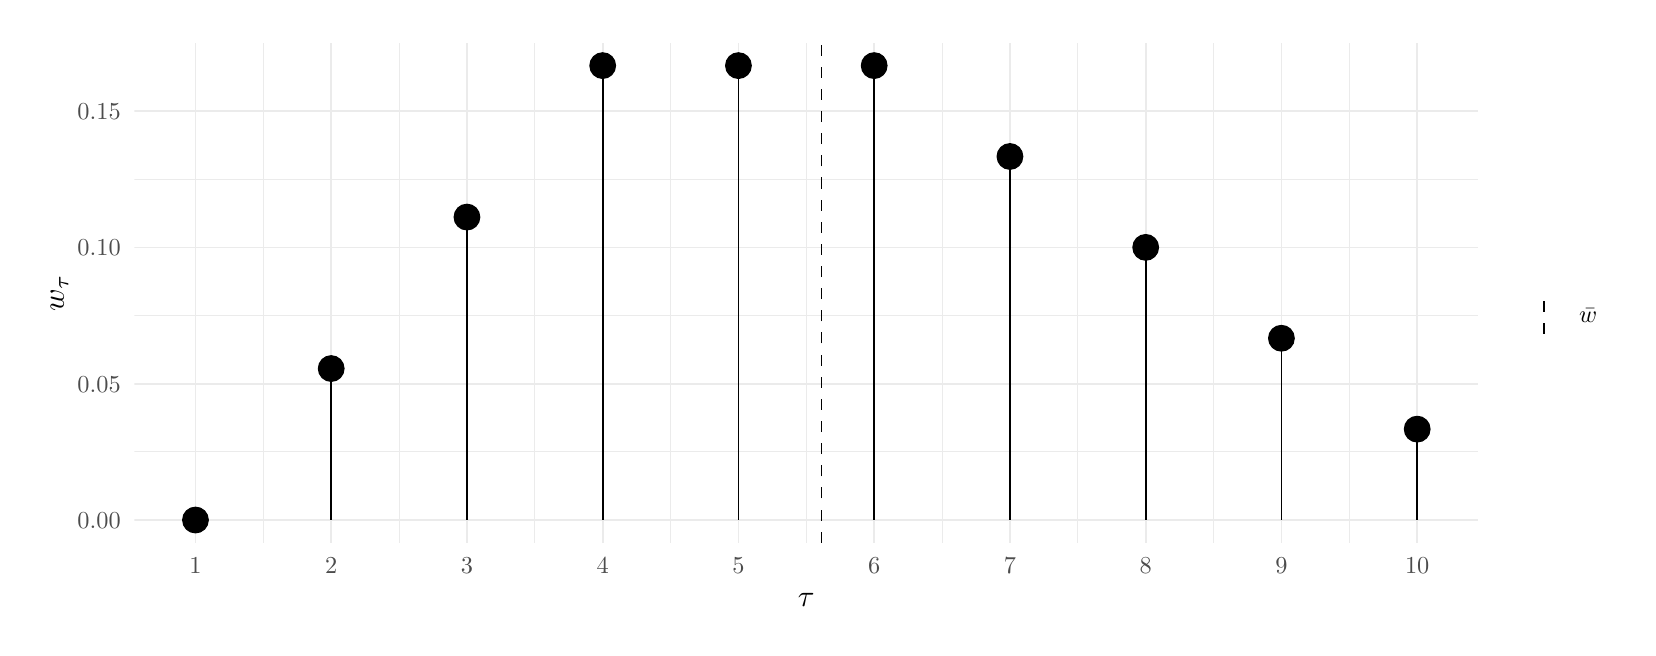
\begin{tikzpicture}[x=1pt,y=1pt]
\definecolor{fillColor}{RGB}{255,255,255}
\path[use as bounding box,fill=fillColor,fill opacity=0.00] (0,0) rectangle (578.16,216.81);
\begin{scope}
\path[clip] ( 38.56, 30.69) rectangle (524.17,211.31);
\definecolor{drawColor}{gray}{0.92}

\path[draw=drawColor,line width= 0.3pt,line join=round] ( 38.56, 63.53) --
	(524.17, 63.53);

\path[draw=drawColor,line width= 0.3pt,line join=round] ( 38.56,112.79) --
	(524.17,112.79);

\path[draw=drawColor,line width= 0.3pt,line join=round] ( 38.56,162.05) --
	(524.17,162.05);

\path[draw=drawColor,line width= 0.3pt,line join=round] ( 85.15, 30.69) --
	( 85.15,211.31);

\path[draw=drawColor,line width= 0.3pt,line join=round] (134.21, 30.69) --
	(134.21,211.31);

\path[draw=drawColor,line width= 0.3pt,line join=round] (183.26, 30.69) --
	(183.26,211.31);

\path[draw=drawColor,line width= 0.3pt,line join=round] (232.31, 30.69) --
	(232.31,211.31);

\path[draw=drawColor,line width= 0.3pt,line join=round] (281.36, 30.69) --
	(281.36,211.31);

\path[draw=drawColor,line width= 0.3pt,line join=round] (330.41, 30.69) --
	(330.41,211.31);

\path[draw=drawColor,line width= 0.3pt,line join=round] (379.47, 30.69) --
	(379.47,211.31);

\path[draw=drawColor,line width= 0.3pt,line join=round] (428.52, 30.69) --
	(428.52,211.31);

\path[draw=drawColor,line width= 0.3pt,line join=round] (477.57, 30.69) --
	(477.57,211.31);

\path[draw=drawColor,line width= 0.6pt,line join=round] ( 38.56, 38.90) --
	(524.17, 38.90);

\path[draw=drawColor,line width= 0.6pt,line join=round] ( 38.56, 88.16) --
	(524.17, 88.16);

\path[draw=drawColor,line width= 0.6pt,line join=round] ( 38.56,137.42) --
	(524.17,137.42);

\path[draw=drawColor,line width= 0.6pt,line join=round] ( 38.56,186.68) --
	(524.17,186.68);

\path[draw=drawColor,line width= 0.6pt,line join=round] ( 60.63, 30.69) --
	( 60.63,211.31);

\path[draw=drawColor,line width= 0.6pt,line join=round] (109.68, 30.69) --
	(109.68,211.31);

\path[draw=drawColor,line width= 0.6pt,line join=round] (158.73, 30.69) --
	(158.73,211.31);

\path[draw=drawColor,line width= 0.6pt,line join=round] (207.78, 30.69) --
	(207.78,211.31);

\path[draw=drawColor,line width= 0.6pt,line join=round] (256.84, 30.69) --
	(256.84,211.31);

\path[draw=drawColor,line width= 0.6pt,line join=round] (305.89, 30.69) --
	(305.89,211.31);

\path[draw=drawColor,line width= 0.6pt,line join=round] (354.94, 30.69) --
	(354.94,211.31);

\path[draw=drawColor,line width= 0.6pt,line join=round] (403.99, 30.69) --
	(403.99,211.31);

\path[draw=drawColor,line width= 0.6pt,line join=round] (453.04, 30.69) --
	(453.04,211.31);

\path[draw=drawColor,line width= 0.6pt,line join=round] (502.10, 30.69) --
	(502.10,211.31);
\definecolor{drawColor}{RGB}{0,0,0}
\definecolor{fillColor}{RGB}{0,0,0}

\path[draw=drawColor,line width= 0.4pt,line join=round,line cap=round,fill=fillColor] ( 60.63, 38.90) circle (  4.64);

\path[draw=drawColor,line width= 0.4pt,line join=round,line cap=round,fill=fillColor] (109.68, 93.63) circle (  4.64);

\path[draw=drawColor,line width= 0.4pt,line join=round,line cap=round,fill=fillColor] (158.73,148.37) circle (  4.64);

\path[draw=drawColor,line width= 0.4pt,line join=round,line cap=round,fill=fillColor] (207.78,203.10) circle (  4.64);

\path[draw=drawColor,line width= 0.4pt,line join=round,line cap=round,fill=fillColor] (256.84,203.10) circle (  4.64);

\path[draw=drawColor,line width= 0.4pt,line join=round,line cap=round,fill=fillColor] (305.89,203.10) circle (  4.64);

\path[draw=drawColor,line width= 0.4pt,line join=round,line cap=round,fill=fillColor] (354.94,170.26) circle (  4.64);

\path[draw=drawColor,line width= 0.4pt,line join=round,line cap=round,fill=fillColor] (403.99,137.42) circle (  4.64);

\path[draw=drawColor,line width= 0.4pt,line join=round,line cap=round,fill=fillColor] (453.04,104.58) circle (  4.64);

\path[draw=drawColor,line width= 0.4pt,line join=round,line cap=round,fill=fillColor] (502.10, 71.74) circle (  4.64);

\path[draw=drawColor,line width= 0.6pt,line join=round] ( 60.63, 38.90) -- ( 60.63, 38.90);

\path[draw=drawColor,line width= 0.6pt,line join=round] (109.68, 93.63) -- (109.68, 38.90);

\path[draw=drawColor,line width= 0.6pt,line join=round] (158.73,148.37) -- (158.73, 38.90);

\path[draw=drawColor,line width= 0.6pt,line join=round] (207.78,203.10) -- (207.78, 38.90);

\path[draw=drawColor,line width= 0.6pt,line join=round] (256.84,203.10) -- (256.84, 38.90);

\path[draw=drawColor,line width= 0.6pt,line join=round] (305.89,203.10) -- (305.89, 38.90);

\path[draw=drawColor,line width= 0.6pt,line join=round] (354.94,170.26) -- (354.94, 38.90);

\path[draw=drawColor,line width= 0.6pt,line join=round] (403.99,137.42) -- (403.99, 38.90);

\path[draw=drawColor,line width= 0.6pt,line join=round] (453.04,104.58) -- (453.04, 38.90);

\path[draw=drawColor,line width= 0.6pt,line join=round] (502.10, 71.74) -- (502.10, 38.90);

\path[draw=drawColor,line width= 0.6pt,dash pattern=on 4pt off 4pt ,line join=round] (286.81, 30.69) -- (286.81,211.31);
\end{scope}
\begin{scope}
\path[clip] (  0.00,  0.00) rectangle (578.16,216.81);
\definecolor{drawColor}{gray}{0.30}

\node[text=drawColor,anchor=base east,inner sep=0pt, outer sep=0pt, scale=  0.88] at ( 33.61, 35.87) {0.00};

\node[text=drawColor,anchor=base east,inner sep=0pt, outer sep=0pt, scale=  0.88] at ( 33.61, 85.13) {0.05};

\node[text=drawColor,anchor=base east,inner sep=0pt, outer sep=0pt, scale=  0.88] at ( 33.61,134.39) {0.10};

\node[text=drawColor,anchor=base east,inner sep=0pt, outer sep=0pt, scale=  0.88] at ( 33.61,183.65) {0.15};
\end{scope}
\begin{scope}
\path[clip] (  0.00,  0.00) rectangle (578.16,216.81);
\definecolor{drawColor}{gray}{0.30}

\node[text=drawColor,anchor=base,inner sep=0pt, outer sep=0pt, scale=  0.88] at ( 60.63, 19.68) {1};

\node[text=drawColor,anchor=base,inner sep=0pt, outer sep=0pt, scale=  0.88] at (109.68, 19.68) {2};

\node[text=drawColor,anchor=base,inner sep=0pt, outer sep=0pt, scale=  0.88] at (158.73, 19.68) {3};

\node[text=drawColor,anchor=base,inner sep=0pt, outer sep=0pt, scale=  0.88] at (207.78, 19.68) {4};

\node[text=drawColor,anchor=base,inner sep=0pt, outer sep=0pt, scale=  0.88] at (256.84, 19.68) {5};

\node[text=drawColor,anchor=base,inner sep=0pt, outer sep=0pt, scale=  0.88] at (305.89, 19.68) {6};

\node[text=drawColor,anchor=base,inner sep=0pt, outer sep=0pt, scale=  0.88] at (354.94, 19.68) {7};

\node[text=drawColor,anchor=base,inner sep=0pt, outer sep=0pt, scale=  0.88] at (403.99, 19.68) {8};

\node[text=drawColor,anchor=base,inner sep=0pt, outer sep=0pt, scale=  0.88] at (453.04, 19.68) {9};

\node[text=drawColor,anchor=base,inner sep=0pt, outer sep=0pt, scale=  0.88] at (502.10, 19.68) {10};
\end{scope}
\begin{scope}
\path[clip] (  0.00,  0.00) rectangle (578.16,216.81);
\definecolor{drawColor}{RGB}{0,0,0}

\node[text=drawColor,anchor=base,inner sep=0pt, outer sep=0pt, scale=  1.10] at (281.36,  7.64) {$\tau$};
\end{scope}
\begin{scope}
\path[clip] (  0.00,  0.00) rectangle (578.16,216.81);
\definecolor{drawColor}{RGB}{0,0,0}

\node[text=drawColor,rotate= 90.00,anchor=base,inner sep=0pt, outer sep=0pt, scale=  1.10] at ( 13.08,121.00) {$w_\tau$};
\end{scope}
\begin{scope}
\path[clip] (  0.00,  0.00) rectangle (578.16,216.81);
\definecolor{drawColor}{RGB}{0,0,0}

\path[draw=drawColor,line width= 0.6pt,dash pattern=on 4pt off 4pt ,line join=round] (547.90,106.16) -- (547.90,120.62);
\end{scope}
\begin{scope}
\path[clip] (  0.00,  0.00) rectangle (578.16,216.81);
\definecolor{drawColor}{RGB}{0,0,0}

\node[text=drawColor,anchor=base west,inner sep=0pt, outer sep=0pt, scale=  0.88] at (560.62,110.36) {$\bar w$};
\end{scope}
\end{tikzpicture}
%
    }
    \caption{Generation time distribution used to estimate reproduction numbers throughout this thesis.}
    \label{fig:generation_time}
\end{figure}

\subsection{Incidence and death data}
In this thesis, we focus on the data available for Germany, provided by the \acrshort{rki} available on zenodo \citep{RobertKoch-Institut2024SARSCoV2} or GitHub \citep{RobertKoch-Institut2024SARSCoV2a}. In these repositories, the \acrshort{rki} publishes daily data on the number of cases in the aforementioned strata. For some days, data have not been published to zenodo, e.g. for May 31st, 2020 \todo{why?}. In this case, we use the data provided by the ard-data RKI-archive on GitHub \citep{MichaelKreil2022RKICoronaDatenArchiv}. 

The \acrshort{rki} data contains for any case and death the following information:
\begin{itemize}
    \item the county (Landkreis) of the case,
    \item sex (male, female or unknown) and age group (00-04, 05-14, 15-34, 35-59, 60-79, 80+, unknown),
    \item the dates of reporting (Meldedatum) and symptom onset (Refdatum), as well as
    \item meta-information whether the case was already present in the past dataset.
\end{itemize}

The dates of reporting and symptom onset are of particular importance: the date of reporting is the date that the local health authorities were made aware of the case, which may be several days after the symptom onset or infection date, but also several days before the \acrshort{rki} is aware of the case. Thus there are several dates of interest, ordered by occurrence (except for the date of death, which could occur before any of the two reporting dates)
\begin{itemize}
    \item the date of infection, 
    \item the date of symptom onset, 
    \item the date of reporting to the local health authorities,
    \item the date of reporting to the \acrshort{rki} and potentially,
    \item the date of death.
\end{itemize}
The date of infection is generally unknown. While the date of symptom onset is close to the date of infection, unfortunately, it is only known for roughly $25\%$ of the reported cases, which is why we restrict our analyses to the date of reporting. \citep{AnDerHeiden2020Schatzung} use multiple imputation to circumvent this problem, however, this method assumes that the symptom onset dates are missing completely at random, which is questionable as, e.g., asymptomatic infections will produce no date of symptom onset. There can be considerable delay between the two reporting dates, as we will explore later, see e.g. \Cref{fig:reporting_delays_cases,fig:survival_function_rep_tri_incidences}.

We restrict ourselves to datasets available from April 1st, 2020, these already include case data on cases with earlier reporting date. \Cref{fig:cases_germany} shows the number of daily reported cases (\textbf{A}) and deaths (\textbf{B}) with a weekly running mean. Apparent from this figure is the considerable day-to-day variation, the so-called week-day effect. As the reporting date is tied to the working hours of the local health authorities, fewer cases are processed, and thus reported, on weekends and more during the week. The week-day effect is less pronounced for the symptom onset date, if it is known (figure not shown). 

We want to highlight two periods of irregularities during the early stage of the epidemic, magnified in \Cref{fig:cases_germany} \textbf{A}. The first concerns a local outbreak in a German meat processing plant \citep{Gunther2020SARSCoV2}. Over two weeks in early June, $1\,413$ positive cases were reported for Gütersloh county. Due to the low number of reported cases everywhere else, this locally confined outbreak is visible even when aggregating over all counties in Germany. \todo{ref this later}
The second period concerns the Christmas holiday break, where we observe a sudden decline in reported cases, compensated by a large influx in cases in the second week of January. Due to the holiday leave, we'd expect this drop in cases to be related to fewer staff working at the local health authorities, rather than a true decrease in cases. Similar patterns are visible for easter 2021 and Christmas 2021. 

\begin{figure}
    \resizebox{\textwidth}{!}{%
        % Created by tikzDevice version 0.12.6 on 2024-08-20 12:05:00
% !TEX encoding = UTF-8 Unicode
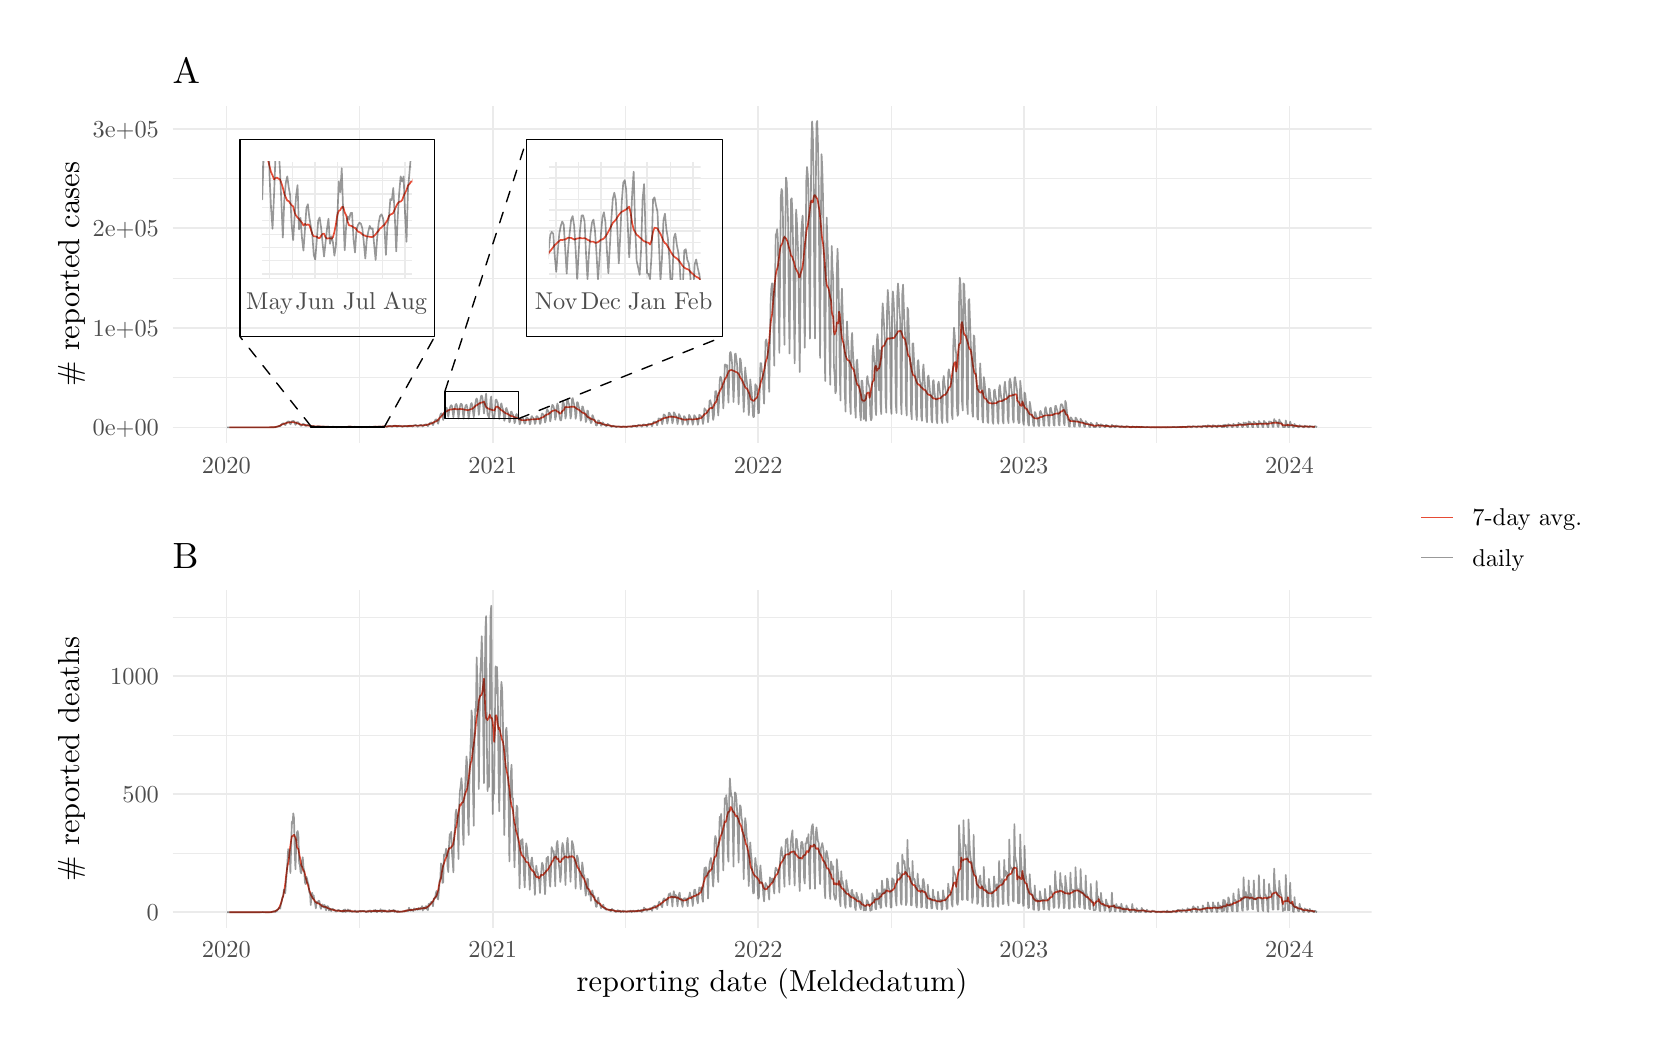
\begin{tikzpicture}[x=1pt,y=1pt]
\definecolor{fillColor}{RGB}{255,255,255}
\path[use as bounding box,fill=fillColor,fill opacity=0.00] (0,0) rectangle (578.16,361.35);
\begin{scope}
\path[clip] ( 52.36,211.36) rectangle (485.62,333.19);
\definecolor{drawColor}{gray}{0.92}

\path[draw=drawColor,line width= 0.3pt,line join=round] ( 52.36,234.90) --
	(485.62,234.90);

\path[draw=drawColor,line width= 0.3pt,line join=round] ( 52.36,270.88) --
	(485.62,270.88);

\path[draw=drawColor,line width= 0.3pt,line join=round] ( 52.36,306.85) --
	(485.62,306.85);

\path[draw=drawColor,line width= 0.3pt,line join=round] (119.91,211.36) --
	(119.91,333.19);

\path[draw=drawColor,line width= 0.3pt,line join=round] (216.01,211.36) --
	(216.01,333.19);

\path[draw=drawColor,line width= 0.3pt,line join=round] (311.98,211.36) --
	(311.98,333.19);

\path[draw=drawColor,line width= 0.3pt,line join=round] (407.95,211.36) --
	(407.95,333.19);

\path[draw=drawColor,line width= 0.6pt,line join=round] ( 52.36,216.92) --
	(485.62,216.92);

\path[draw=drawColor,line width= 0.6pt,line join=round] ( 52.36,252.89) --
	(485.62,252.89);

\path[draw=drawColor,line width= 0.6pt,line join=round] ( 52.36,288.86) --
	(485.62,288.86);

\path[draw=drawColor,line width= 0.6pt,line join=round] ( 52.36,324.84) --
	(485.62,324.84);

\path[draw=drawColor,line width= 0.6pt,line join=round] ( 71.79,211.36) --
	( 71.79,333.19);

\path[draw=drawColor,line width= 0.6pt,line join=round] (168.03,211.36) --
	(168.03,333.19);

\path[draw=drawColor,line width= 0.6pt,line join=round] (263.99,211.36) --
	(263.99,333.19);

\path[draw=drawColor,line width= 0.6pt,line join=round] (359.96,211.36) --
	(359.96,333.19);

\path[draw=drawColor,line width= 0.6pt,line join=round] (455.93,211.36) --
	(455.93,333.19);
\definecolor{drawColor}{RGB}{230,75,53}

\path[draw=drawColor,line width= 0.6pt,line join=round] ( 72.85,216.92) --
	( 73.11,216.92) --
	( 73.37,216.92) --
	( 73.63,216.92) --
	( 73.90,216.92) --
	( 74.16,216.92) --
	( 74.42,216.92) --
	( 74.69,216.92) --
	( 74.95,216.92) --
	( 75.21,216.92) --
	( 75.48,216.92) --
	( 75.74,216.92) --
	( 76.00,216.92) --
	( 76.26,216.92) --
	( 76.53,216.92) --
	( 76.79,216.92) --
	( 77.05,216.92) --
	( 77.32,216.92) --
	( 77.58,216.92) --
	( 77.84,216.92) --
	( 78.10,216.92) --
	( 78.37,216.92) --
	( 78.63,216.92) --
	( 78.89,216.92) --
	( 79.16,216.92) --
	( 79.42,216.92) --
	( 79.68,216.92) --
	( 79.95,216.92) --
	( 80.21,216.92) --
	( 80.47,216.92) --
	( 80.73,216.92) --
	( 81.00,216.92) --
	( 81.26,216.92) --
	( 81.52,216.92) --
	( 81.79,216.92) --
	( 82.05,216.92) --
	( 82.31,216.92) --
	( 82.57,216.92) --
	( 82.84,216.92) --
	( 83.10,216.92) --
	( 83.36,216.92) --
	( 83.63,216.92) --
	( 83.89,216.92) --
	( 84.15,216.92) --
	( 84.41,216.92) --
	( 84.68,216.92) --
	( 84.94,216.92) --
	( 85.20,216.92) --
	( 85.47,216.92) --
	( 85.73,216.92) --
	( 85.99,216.92) --
	( 86.26,216.92) --
	( 86.52,216.92) --
	( 86.78,216.92) --
	( 87.04,216.93) --
	( 87.31,216.93) --
	( 87.57,216.94) --
	( 87.83,216.95) --
	( 88.10,216.95) --
	( 88.36,216.96) --
	( 88.62,216.96) --
	( 88.88,216.98) --
	( 89.15,217.01) --
	( 89.41,217.04) --
	( 89.67,217.08) --
	( 89.94,217.14) --
	( 90.20,217.20) --
	( 90.46,217.25) --
	( 90.73,217.33) --
	( 90.99,217.46) --
	( 91.25,217.61) --
	( 91.51,217.76) --
	( 91.78,217.90) --
	( 92.04,218.00) --
	( 92.30,218.07) --
	( 92.57,218.16) --
	( 92.83,218.25) --
	( 93.09,218.36) --
	( 93.35,218.45) --
	( 93.62,218.55) --
	( 93.88,218.62) --
	( 94.14,218.66) --
	( 94.41,218.68) --
	( 94.67,218.74) --
	( 94.93,218.77) --
	( 95.19,218.81) --
	( 95.46,218.82) --
	( 95.72,218.80) --
	( 95.98,218.77) --
	( 96.25,218.75) --
	( 96.51,218.70) --
	( 96.77,218.65) --
	( 97.04,218.57) --
	( 97.30,218.42) --
	( 97.56,218.35) --
	( 97.82,218.31) --
	( 98.09,218.21) --
	( 98.35,218.07) --
	( 98.61,217.97) --
	( 98.88,217.89) --
	( 99.14,217.87) --
	( 99.40,217.83) --
	( 99.66,217.81) --
	( 99.93,217.81) --
	(100.19,217.80) --
	(100.45,217.76) --
	(100.72,217.69) --
	(100.98,217.63) --
	(101.24,217.59) --
	(101.51,217.55) --
	(101.77,217.52) --
	(102.03,217.48) --
	(102.29,217.43) --
	(102.56,217.40) --
	(102.82,217.35) --
	(103.08,217.31) --
	(103.35,217.30) --
	(103.61,217.28) --
	(103.87,217.26) --
	(104.13,217.25) --
	(104.40,217.24) --
	(104.66,217.24) --
	(104.92,217.24) --
	(105.19,217.24) --
	(105.45,217.24) --
	(105.71,217.22) --
	(105.97,217.21) --
	(106.24,217.19) --
	(106.50,217.17) --
	(106.76,217.16) --
	(107.03,217.16) --
	(107.29,217.15) --
	(107.55,217.15) --
	(107.82,217.14) --
	(108.08,217.12) --
	(108.34,217.11) --
	(108.60,217.11) --
	(108.87,217.10) --
	(109.13,217.10) --
	(109.39,217.09) --
	(109.66,217.08) --
	(109.92,217.09) --
	(110.18,217.08) --
	(110.44,217.08) --
	(110.71,217.08) --
	(110.97,217.07) --
	(111.23,217.05) --
	(111.50,217.04) --
	(111.76,217.04) --
	(112.02,217.04) --
	(112.29,217.04) --
	(112.55,217.04) --
	(112.81,217.05) --
	(113.07,217.05) --
	(113.34,217.05) --
	(113.60,217.04) --
	(113.86,217.04) --
	(114.13,217.04) --
	(114.39,217.04) --
	(114.65,217.04) --
	(114.91,217.04) --
	(115.18,217.06) --
	(115.44,217.08) --
	(115.70,217.12) --
	(115.97,217.13) --
	(116.23,217.13) --
	(116.49,217.14) --
	(116.76,217.14) --
	(117.02,217.12) --
	(117.28,217.11) --
	(117.54,217.09) --
	(117.81,217.08) --
	(118.07,217.08) --
	(118.33,217.08) --
	(118.60,217.07) --
	(118.86,217.07) --
	(119.12,217.07) --
	(119.38,217.06) --
	(119.65,217.06) --
	(119.91,217.05) --
	(120.17,217.05) --
	(120.44,217.05) --
	(120.70,217.05) --
	(120.96,217.04) --
	(121.22,217.04) --
	(121.49,217.04) --
	(121.75,217.04) --
	(122.01,217.04) --
	(122.28,217.05) --
	(122.54,217.05) --
	(122.80,217.06) --
	(123.07,217.06) --
	(123.33,217.07) --
	(123.59,217.07) --
	(123.85,217.08) --
	(124.12,217.08) --
	(124.38,217.09) --
	(124.64,217.10) --
	(124.91,217.11) --
	(125.17,217.12) --
	(125.43,217.12) --
	(125.69,217.12) --
	(125.96,217.13) --
	(126.22,217.15) --
	(126.48,217.15) --
	(126.75,217.16) --
	(127.01,217.16) --
	(127.27,217.17) --
	(127.54,217.18) --
	(127.80,217.19) --
	(128.06,217.20) --
	(128.32,217.22) --
	(128.59,217.22) --
	(128.85,217.23) --
	(129.11,217.23) --
	(129.38,217.24) --
	(129.64,217.26) --
	(129.90,217.28) --
	(130.16,217.30) --
	(130.43,217.31) --
	(130.69,217.32) --
	(130.95,217.33) --
	(131.22,217.35) --
	(131.48,217.37) --
	(131.74,217.38) --
	(132.00,217.38) --
	(132.27,217.40) --
	(132.53,217.41) --
	(132.79,217.41) --
	(133.06,217.40) --
	(133.32,217.40) --
	(133.58,217.39) --
	(133.85,217.39) --
	(134.11,217.38) --
	(134.37,217.37) --
	(134.63,217.37) --
	(134.90,217.36) --
	(135.16,217.35) --
	(135.42,217.34) --
	(135.69,217.34) --
	(135.95,217.34) --
	(136.21,217.36) --
	(136.47,217.36) --
	(136.74,217.37) --
	(137.00,217.37) --
	(137.26,217.39) --
	(137.53,217.40) --
	(137.79,217.40) --
	(138.05,217.41) --
	(138.32,217.42) --
	(138.58,217.42) --
	(138.84,217.46) --
	(139.10,217.48) --
	(139.37,217.52) --
	(139.63,217.54) --
	(139.89,217.55) --
	(140.16,217.55) --
	(140.42,217.56) --
	(140.68,217.55) --
	(140.94,217.55) --
	(141.21,217.55) --
	(141.47,217.56) --
	(141.73,217.58) --
	(142.00,217.59) --
	(142.26,217.60) --
	(142.52,217.61) --
	(142.78,217.64) --
	(143.05,217.67) --
	(143.31,217.70) --
	(143.57,217.72) --
	(143.84,217.74) --
	(144.10,217.77) --
	(144.36,217.84) --
	(144.63,217.93) --
	(144.89,218.02) --
	(145.15,218.13) --
	(145.41,218.20) --
	(145.68,218.26) --
	(145.94,218.35) --
	(146.20,218.44) --
	(146.47,218.58) --
	(146.73,218.75) --
	(146.99,218.90) --
	(147.25,219.00) --
	(147.52,219.08) --
	(147.78,219.19) --
	(148.04,219.40) --
	(148.31,219.67) --
	(148.57,219.98) --
	(148.83,220.29) --
	(149.10,220.57) --
	(149.36,220.76) --
	(149.62,221.05) --
	(149.88,221.38) --
	(150.15,221.73) --
	(150.41,222.04) --
	(150.67,222.31) --
	(150.94,222.46) --
	(151.20,222.62) --
	(151.46,222.79) --
	(151.72,222.96) --
	(151.99,223.06) --
	(152.25,223.19) --
	(152.51,223.30) --
	(152.78,223.40) --
	(153.04,223.38) --
	(153.30,223.41) --
	(153.56,223.43) --
	(153.83,223.51) --
	(154.09,223.57) --
	(154.35,223.56) --
	(154.62,223.55) --
	(154.88,223.49) --
	(155.14,223.42) --
	(155.41,223.46) --
	(155.67,223.51) --
	(155.93,223.52) --
	(156.19,223.57) --
	(156.46,223.52) --
	(156.72,223.52) --
	(156.98,223.53) --
	(157.25,223.48) --
	(157.51,223.40) --
	(157.77,223.35) --
	(158.03,223.24) --
	(158.30,223.25) --
	(158.56,223.24) --
	(158.82,223.15) --
	(159.09,223.15) --
	(159.35,223.21) --
	(159.61,223.29) --
	(159.88,223.40) --
	(160.14,223.44) --
	(160.40,223.51) --
	(160.66,223.67) --
	(160.93,223.85) --
	(161.19,224.08) --
	(161.45,224.31) --
	(161.72,224.58) --
	(161.98,224.83) --
	(162.24,224.95) --
	(162.50,225.08) --
	(162.77,225.29) --
	(163.03,225.48) --
	(163.29,225.63) --
	(163.56,225.76) --
	(163.82,225.82) --
	(164.08,225.89) --
	(164.34,225.95) --
	(164.61,226.06) --
	(164.87,226.19) --
	(165.13,225.63) --
	(165.40,224.78) --
	(165.66,224.26) --
	(165.92,224.05) --
	(166.19,223.81) --
	(166.45,223.74) --
	(166.71,223.59) --
	(166.97,223.51) --
	(167.24,223.36) --
	(167.50,223.28) --
	(167.76,223.23) --
	(168.03,223.16) --
	(168.29,223.16) --
	(168.55,223.00) --
	(168.81,223.33) --
	(169.08,224.07) --
	(169.34,224.41) --
	(169.60,224.39) --
	(169.87,224.35) --
	(170.13,224.10) --
	(170.39,223.90) --
	(170.66,223.61) --
	(170.92,223.29) --
	(171.18,223.12) --
	(171.44,223.03) --
	(171.71,222.81) --
	(171.97,222.59) --
	(172.23,222.36) --
	(172.50,222.17) --
	(172.76,222.00) --
	(173.02,221.91) --
	(173.28,221.83) --
	(173.55,221.70) --
	(173.81,221.55) --
	(174.07,221.36) --
	(174.34,221.19) --
	(174.60,221.06) --
	(174.86,220.98) --
	(175.12,220.93) --
	(175.39,220.89) --
	(175.65,220.72) --
	(175.91,220.60) --
	(176.18,220.50) --
	(176.44,220.37) --
	(176.70,220.29) --
	(176.97,220.24) --
	(177.23,220.15) --
	(177.49,219.99) --
	(177.75,219.82) --
	(178.02,219.71) --
	(178.28,219.64) --
	(178.54,219.49) --
	(178.81,219.53) --
	(179.07,219.54) --
	(179.33,219.55) --
	(179.59,219.53) --
	(179.86,219.52) --
	(180.12,219.53) --
	(180.38,219.64) --
	(180.65,219.61) --
	(180.91,219.61) --
	(181.17,219.65) --
	(181.44,219.72) --
	(181.70,219.76) --
	(181.96,219.80) --
	(182.22,219.79) --
	(182.49,219.81) --
	(182.75,219.83) --
	(183.01,219.87) --
	(183.28,219.87) --
	(183.54,219.88) --
	(183.80,219.89) --
	(184.06,219.92) --
	(184.33,219.92) --
	(184.59,219.93) --
	(184.85,219.96) --
	(185.12,220.09) --
	(185.38,220.25) --
	(185.64,220.40) --
	(185.90,220.51) --
	(186.17,220.59) --
	(186.43,220.69) --
	(186.69,220.91) --
	(186.96,221.13) --
	(187.22,221.32) --
	(187.48,221.48) --
	(187.75,221.62) --
	(188.01,221.68) --
	(188.27,221.78) --
	(188.53,221.97) --
	(188.80,222.19) --
	(189.06,222.46) --
	(189.32,222.68) --
	(189.59,222.81) --
	(189.85,222.89) --
	(190.11,223.00) --
	(190.37,223.05) --
	(190.64,223.12) --
	(190.90,223.09) --
	(191.16,222.86) --
	(191.43,222.59) --
	(191.69,222.57) --
	(191.95,222.37) --
	(192.22,221.91) --
	(192.48,221.90) --
	(192.74,222.12) --
	(193.00,222.52) --
	(193.27,222.90) --
	(193.53,222.99) --
	(193.79,223.25) --
	(194.06,224.03) --
	(194.32,224.28) --
	(194.58,224.25) --
	(194.84,224.24) --
	(195.11,224.22) --
	(195.37,224.22) --
	(195.63,224.22) --
	(195.90,224.29) --
	(196.16,224.33) --
	(196.42,224.35) --
	(196.68,224.34) --
	(196.95,224.36) --
	(197.21,224.35) --
	(197.47,224.35) --
	(197.74,224.21) --
	(198.00,223.98) --
	(198.26,223.77) --
	(198.53,223.58) --
	(198.79,223.43) --
	(199.05,223.32) --
	(199.31,223.17) --
	(199.58,222.95) --
	(199.84,222.73) --
	(200.10,222.51) --
	(200.37,222.32) --
	(200.63,222.17) --
	(200.89,222.10) --
	(201.15,222.01) --
	(201.42,221.79) --
	(201.68,221.57) --
	(201.94,221.18) --
	(202.21,220.78) --
	(202.47,220.61) --
	(202.73,220.55) --
	(203.00,220.44) --
	(203.26,220.21) --
	(203.52,219.95) --
	(203.78,219.89) --
	(204.05,219.88) --
	(204.31,219.74) --
	(204.57,219.62) --
	(204.84,219.45) --
	(205.10,219.00) --
	(205.36,218.79) --
	(205.62,218.70) --
	(205.89,218.58) --
	(206.15,218.47) --
	(206.41,218.45) --
	(206.68,218.48) --
	(206.94,218.56) --
	(207.20,218.42) --
	(207.46,218.22) --
	(207.73,218.07) --
	(207.99,218.00) --
	(208.25,217.98) --
	(208.52,217.94) --
	(208.78,217.86) --
	(209.04,217.78) --
	(209.31,217.74) --
	(209.57,217.72) --
	(209.83,217.67) --
	(210.09,217.64) --
	(210.36,217.60) --
	(210.62,217.50) --
	(210.88,217.43) --
	(211.15,217.37) --
	(211.41,217.33) --
	(211.67,217.30) --
	(211.93,217.29) --
	(212.20,217.27) --
	(212.46,217.24) --
	(212.72,217.21) --
	(212.99,217.20) --
	(213.25,217.18) --
	(213.51,217.17) --
	(213.78,217.17) --
	(214.04,217.16) --
	(214.30,217.15) --
	(214.56,217.15) --
	(214.83,217.15) --
	(215.09,217.14) --
	(215.35,217.14) --
	(215.62,217.14) --
	(215.88,217.14) --
	(216.14,217.15) --
	(216.40,217.16) --
	(216.67,217.17) --
	(216.93,217.18) --
	(217.19,217.20) --
	(217.46,217.20) --
	(217.72,217.22) --
	(217.98,217.25) --
	(218.24,217.29) --
	(218.51,217.32) --
	(218.77,217.35) --
	(219.03,217.38) --
	(219.30,217.38) --
	(219.56,217.42) --
	(219.82,217.45) --
	(220.09,217.48) --
	(220.35,217.52) --
	(220.61,217.54) --
	(220.87,217.56) --
	(221.14,217.57) --
	(221.40,217.58) --
	(221.66,217.62) --
	(221.93,217.65) --
	(222.19,217.67) --
	(222.45,217.69) --
	(222.71,217.71) --
	(222.98,217.71) --
	(223.24,217.74) --
	(223.50,217.77) --
	(223.77,217.81) --
	(224.03,217.85) --
	(224.29,217.91) --
	(224.56,217.95) --
	(224.82,217.97) --
	(225.08,218.01) --
	(225.34,218.10) --
	(225.61,218.21) --
	(225.87,218.31) --
	(226.13,218.42) --
	(226.40,218.52) --
	(226.66,218.57) --
	(226.92,218.65) --
	(227.18,218.82) --
	(227.45,218.98) --
	(227.71,219.15) --
	(227.97,219.30) --
	(228.24,219.42) --
	(228.50,219.47) --
	(228.76,219.57) --
	(229.02,219.78) --
	(229.29,219.98) --
	(229.55,220.13) --
	(229.81,220.21) --
	(230.08,220.29) --
	(230.34,220.33) --
	(230.60,220.35) --
	(230.87,220.44) --
	(231.13,220.54) --
	(231.39,220.60) --
	(231.65,220.69) --
	(231.92,220.74) --
	(232.18,220.76) --
	(232.44,220.75) --
	(232.71,220.78) --
	(232.97,220.75) --
	(233.23,220.73) --
	(233.49,220.69) --
	(233.76,220.64) --
	(234.02,220.60) --
	(234.28,220.59) --
	(234.55,220.50) --
	(234.81,220.40) --
	(235.07,220.29) --
	(235.34,220.18) --
	(235.60,220.10) --
	(235.86,220.08) --
	(236.12,220.00) --
	(236.39,219.89) --
	(236.65,219.80) --
	(236.91,219.74) --
	(237.18,219.71) --
	(237.44,219.68) --
	(237.70,219.67) --
	(237.96,219.69) --
	(238.23,219.76) --
	(238.49,219.81) --
	(238.75,219.83) --
	(239.02,219.83) --
	(239.28,219.82) --
	(239.54,219.82) --
	(239.80,219.81) --
	(240.07,219.79) --
	(240.33,219.78) --
	(240.59,219.81) --
	(240.86,219.85) --
	(241.12,219.90) --
	(241.38,219.90) --
	(241.65,219.93) --
	(241.91,219.95) --
	(242.17,220.00) --
	(242.43,220.06) --
	(242.70,220.16) --
	(242.96,220.24) --
	(243.22,220.28) --
	(243.49,220.37) --
	(243.75,220.71) --
	(244.01,221.01) --
	(244.27,221.32) --
	(244.54,221.60) --
	(244.80,221.85) --
	(245.06,221.94) --
	(245.33,222.13) --
	(245.59,222.50) --
	(245.85,222.98) --
	(246.12,223.34) --
	(246.38,223.65) --
	(246.64,223.84) --
	(246.90,223.96) --
	(247.17,223.94) --
	(247.43,223.84) --
	(247.69,224.29) --
	(247.96,224.91) --
	(248.22,225.49) --
	(248.48,225.83) --
	(248.74,226.06) --
	(249.01,226.72) --
	(249.27,227.89) --
	(249.53,228.64) --
	(249.80,229.32) --
	(250.06,229.96) --
	(250.32,230.48) --
	(250.58,230.85) --
	(250.85,231.38) --
	(251.11,232.19) --
	(251.37,232.83) --
	(251.64,233.42) --
	(251.90,234.26) --
	(252.16,234.69) --
	(252.43,234.99) --
	(252.69,235.61) --
	(252.95,236.20) --
	(253.21,236.85) --
	(253.48,237.39) --
	(253.74,237.47) --
	(254.00,237.60) --
	(254.27,237.64) --
	(254.53,237.53) --
	(254.79,237.48) --
	(255.05,237.39) --
	(255.32,237.19) --
	(255.58,237.11) --
	(255.84,236.99) --
	(256.11,236.86) --
	(256.37,236.76) --
	(256.63,236.54) --
	(256.90,236.19) --
	(257.16,235.66) --
	(257.42,235.08) --
	(257.68,234.67) --
	(257.95,234.29) --
	(258.21,233.73) --
	(258.47,233.26) --
	(258.74,232.50) --
	(259.00,231.96) --
	(259.26,231.46) --
	(259.52,231.14) --
	(259.79,230.97) --
	(260.05,230.73) --
	(260.31,230.12) --
	(260.58,229.53) --
	(260.84,228.90) --
	(261.10,227.90) --
	(261.36,226.97) --
	(261.63,226.88) --
	(261.89,226.75) --
	(262.15,226.50) --
	(262.42,226.54) --
	(262.68,226.87) --
	(262.94,227.23) --
	(263.21,227.43) --
	(263.47,227.64) --
	(263.73,228.23) --
	(263.99,229.32) --
	(264.26,230.49) --
	(264.52,231.26) --
	(264.78,232.64) --
	(265.05,233.81) --
	(265.31,234.28) --
	(265.57,235.20) --
	(265.83,236.30) --
	(266.10,237.53) --
	(266.36,238.96) --
	(266.62,240.24) --
	(266.89,241.29) --
	(267.15,241.90) --
	(267.41,243.39) --
	(267.68,245.48) --
	(267.94,248.14) --
	(268.20,251.25) --
	(268.46,254.51) --
	(268.73,256.51) --
	(268.99,257.86) --
	(269.25,260.77) --
	(269.52,264.20) --
	(269.78,267.01) --
	(270.04,269.81) --
	(270.30,272.06) --
	(270.57,273.53) --
	(270.83,274.19) --
	(271.09,275.21) --
	(271.36,277.13) --
	(271.62,279.42) --
	(271.88,281.38) --
	(272.14,282.50) --
	(272.41,282.94) --
	(272.67,283.35) --
	(272.93,284.32) --
	(273.20,285.36) --
	(273.46,285.76) --
	(273.72,285.40) --
	(273.99,285.24) --
	(274.25,284.69) --
	(274.51,284.24) --
	(274.77,283.25) --
	(275.04,282.11) --
	(275.30,281.23) --
	(275.56,280.36) --
	(275.83,278.94) --
	(276.09,278.81) --
	(276.35,278.30) --
	(276.61,277.31) --
	(276.88,276.80) --
	(277.14,275.67) --
	(277.40,274.48) --
	(277.67,274.10) --
	(277.93,273.53) --
	(278.19,273.08) --
	(278.46,272.52) --
	(278.72,271.24) --
	(278.98,271.10) --
	(279.24,272.27) --
	(279.51,273.22) --
	(279.77,273.92) --
	(280.03,275.17) --
	(280.30,277.08) --
	(280.56,279.86) --
	(280.82,282.74) --
	(281.08,284.88) --
	(281.35,287.38) --
	(281.61,289.10) --
	(281.87,289.57) --
	(282.14,291.73) --
	(282.40,293.64) --
	(282.66,295.99) --
	(282.92,298.07) --
	(283.19,298.89) --
	(283.45,298.23) --
	(283.71,298.25) --
	(283.98,299.78) --
	(284.24,300.79) --
	(284.50,300.82) --
	(284.77,300.37) --
	(285.03,299.83) --
	(285.29,299.58) --
	(285.55,298.57) --
	(285.82,296.98) --
	(286.08,295.42) --
	(286.34,292.95) --
	(286.61,290.17) --
	(286.87,286.97) --
	(287.13,284.65) --
	(287.39,283.46) --
	(287.66,280.81) --
	(287.92,277.55) --
	(288.18,273.90) --
	(288.45,270.60) --
	(288.71,268.58) --
	(288.97,267.71) --
	(289.24,267.51) --
	(289.50,266.74) --
	(289.76,265.27) --
	(290.02,263.72) --
	(290.29,262.84) --
	(290.55,258.63) --
	(290.81,257.39) --
	(291.08,256.96) --
	(291.34,251.64) --
	(291.60,250.44) --
	(291.86,251.49) --
	(292.13,251.75) --
	(292.39,254.76) --
	(292.65,254.89) --
	(292.92,254.51) --
	(293.18,258.72) --
	(293.44,257.73) --
	(293.70,254.44) --
	(293.97,251.31) --
	(294.23,249.19) --
	(294.49,248.14) --
	(294.76,247.57) --
	(295.02,245.91) --
	(295.28,244.22) --
	(295.55,242.90) --
	(295.81,242.17) --
	(296.07,241.59) --
	(296.33,241.23) --
	(296.60,241.11) --
	(296.86,241.02) --
	(297.12,240.42) --
	(297.39,239.77) --
	(297.65,238.98) --
	(297.91,238.45) --
	(298.17,238.10) --
	(298.44,237.91) --
	(298.70,236.92) --
	(298.96,235.54) --
	(299.23,234.34) --
	(299.49,233.28) --
	(299.75,232.41) --
	(300.02,232.08) --
	(300.28,231.95) --
	(300.54,230.99) --
	(300.80,229.89) --
	(301.07,228.95) --
	(301.33,227.10) --
	(301.59,226.72) --
	(301.86,226.56) --
	(302.12,226.53) --
	(302.38,226.52) --
	(302.64,226.77) --
	(302.91,227.27) --
	(303.17,229.02) --
	(303.43,229.37) --
	(303.70,229.48) --
	(303.96,229.51) --
	(304.22,227.58) --
	(304.48,228.60) --
	(304.75,230.51) --
	(305.01,231.99) --
	(305.27,233.32) --
	(305.54,233.68) --
	(305.80,233.95) --
	(306.06,237.94) --
	(306.33,239.08) --
	(306.59,239.07) --
	(306.85,237.33) --
	(307.11,237.96) --
	(307.38,238.13) --
	(307.64,238.18) --
	(307.90,239.13) --
	(308.17,240.72) --
	(308.43,242.35) --
	(308.69,245.64) --
	(308.95,246.14) --
	(309.22,246.35) --
	(309.48,246.42) --
	(309.74,247.01) --
	(310.01,247.70) --
	(310.27,248.30) --
	(310.53,248.75) --
	(310.80,249.15) --
	(311.06,248.98) --
	(311.32,248.92) --
	(311.58,249.12) --
	(311.85,249.04) --
	(312.11,249.16) --
	(312.37,249.19) --
	(312.64,249.23) --
	(312.90,249.21) --
	(313.16,249.25) --
	(313.42,249.78) --
	(313.69,250.19) --
	(313.95,250.61) --
	(314.21,250.92) --
	(314.48,251.59) --
	(314.74,251.67) --
	(315.00,251.61) --
	(315.26,251.78) --
	(315.53,251.72) --
	(315.79,251.03) --
	(316.05,250.35) --
	(316.32,249.36) --
	(316.58,249.21) --
	(316.84,249.15) --
	(317.11,248.42) --
	(317.37,247.12) --
	(317.63,245.79) --
	(317.89,244.34) --
	(318.16,242.93) --
	(318.42,242.59) --
	(318.68,242.39) --
	(318.95,240.54) --
	(319.21,238.80) --
	(319.47,237.40) --
	(319.73,236.42) --
	(320.00,235.73) --
	(320.26,235.61) --
	(320.52,235.57) --
	(320.79,234.65) --
	(321.05,233.78) --
	(321.31,233.12) --
	(321.58,232.66) --
	(321.84,232.40) --
	(322.10,232.28) --
	(322.36,232.25) --
	(322.63,231.64) --
	(322.89,231.42) --
	(323.15,231.23) --
	(323.42,231.00) --
	(323.68,230.60) --
	(323.94,230.52) --
	(324.20,230.45) --
	(324.47,230.24) --
	(324.73,229.68) --
	(324.99,229.25) --
	(325.26,228.89) --
	(325.52,228.72) --
	(325.78,228.64) --
	(326.04,228.63) --
	(326.31,228.41) --
	(326.57,228.18) --
	(326.83,227.80) --
	(327.10,227.52) --
	(327.36,227.33) --
	(327.62,227.32) --
	(327.89,227.28) --
	(328.15,227.12) --
	(328.41,227.04) --
	(328.67,227.17) --
	(328.94,227.33) --
	(329.20,227.41) --
	(329.46,227.39) --
	(329.73,227.40) --
	(329.99,227.62) --
	(330.25,227.92) --
	(330.51,228.09) --
	(330.78,228.38) --
	(331.04,228.62) --
	(331.30,228.65) --
	(331.57,228.68) --
	(331.83,229.08) --
	(332.09,229.42) --
	(332.36,229.99) --
	(332.62,230.51) --
	(332.88,231.18) --
	(333.14,231.47) --
	(333.41,231.64) --
	(333.67,232.99) --
	(333.93,235.14) --
	(334.20,237.13) --
	(334.46,238.62) --
	(334.72,239.96) --
	(334.98,240.33) --
	(335.25,240.50) --
	(335.51,237.07) --
	(335.77,238.46) --
	(336.04,241.44) --
	(336.30,244.74) --
	(336.56,246.87) --
	(336.82,247.16) --
	(337.09,247.45) --
	(337.35,254.13) --
	(337.61,254.97) --
	(337.88,253.63) --
	(338.14,251.76) --
	(338.40,250.50) --
	(338.67,250.28) --
	(338.93,250.09) --
	(339.19,249.19) --
	(339.45,248.43) --
	(339.72,247.52) --
	(339.98,246.42) --
	(340.24,245.35) --
	(340.51,245.08) --
	(340.77,244.94) --
	(341.03,243.16) --
	(341.29,241.23) --
	(341.56,239.33) --
	(341.82,237.86) --
	(342.08,236.61) --
	(342.35,236.28) --
	(342.61,236.13) --
	(342.87,233.52) --
	(343.14,230.78) --
	(343.40,230.50) --
	(343.66,230.12) --
	(343.92,229.70) --
	(344.19,229.59) --
	(344.45,229.43) --
	(344.71,229.89) --
	(344.98,230.28) --
	(345.24,228.88) --
	(345.50,227.96) --
	(345.76,227.43) --
	(346.03,227.31) --
	(346.29,227.30) --
	(346.55,226.70) --
	(346.82,226.31) --
	(347.08,225.97) --
	(347.34,225.76) --
	(347.61,225.68) --
	(347.87,225.68) --
	(348.13,225.64) --
	(348.39,225.51) --
	(348.66,225.51) --
	(348.92,225.58) --
	(349.18,225.64) --
	(349.45,225.66) --
	(349.71,225.68) --
	(349.97,225.68) --
	(350.23,225.83) --
	(350.50,226.07) --
	(350.76,226.22) --
	(351.02,226.31) --
	(351.29,226.39) --
	(351.55,226.40) --
	(351.81,226.41) --
	(352.07,226.42) --
	(352.34,226.59) --
	(352.60,226.74) --
	(352.86,226.93) --
	(353.13,227.06) --
	(353.39,227.15) --
	(353.65,227.17) --
	(353.92,227.50) --
	(354.18,227.65) --
	(354.44,228.02) --
	(354.70,228.26) --
	(354.97,228.36) --
	(355.23,228.35) --
	(355.49,228.37) --
	(355.76,228.53) --
	(356.02,228.62) --
	(356.28,228.62) --
	(356.54,228.74) --
	(356.81,228.86) --
	(357.07,228.84) --
	(357.33,228.82) --
	(357.60,226.53) --
	(357.86,226.35) --
	(358.12,226.08) --
	(358.39,225.55) --
	(358.65,224.95) --
	(358.91,224.80) --
	(359.17,224.71) --
	(359.44,226.26) --
	(359.70,225.57) --
	(359.96,224.80) --
	(360.23,224.29) --
	(360.49,223.75) --
	(360.75,223.66) --
	(361.01,223.61) --
	(361.28,223.14) --
	(361.54,222.55) --
	(361.80,222.12) --
	(362.07,221.70) --
	(362.33,221.55) --
	(362.59,221.51) --
	(362.85,221.49) --
	(363.12,220.96) --
	(363.38,220.58) --
	(363.64,220.32) --
	(363.91,220.21) --
	(364.17,220.16) --
	(364.43,220.15) --
	(364.70,220.15) --
	(364.96,220.13) --
	(365.22,220.24) --
	(365.48,220.38) --
	(365.75,220.53) --
	(366.01,220.65) --
	(366.27,220.67) --
	(366.54,220.68) --
	(366.80,220.85) --
	(367.06,221.04) --
	(367.32,221.15) --
	(367.59,221.18) --
	(367.85,221.25) --
	(368.11,221.25) --
	(368.38,221.25) --
	(368.64,221.28) --
	(368.90,221.24) --
	(369.17,221.26) --
	(369.43,221.29) --
	(369.69,221.34) --
	(369.95,221.36) --
	(370.22,221.37) --
	(370.48,221.49) --
	(370.74,221.59) --
	(371.01,221.72) --
	(371.27,221.87) --
	(371.53,221.91) --
	(371.79,221.93) --
	(372.06,221.95) --
	(372.32,221.82) --
	(372.58,221.91) --
	(372.85,222.13) --
	(373.11,222.41) --
	(373.37,222.67) --
	(373.63,222.74) --
	(373.90,222.75) --
	(374.16,223.15) --
	(374.42,223.20) --
	(374.69,222.89) --
	(374.95,222.21) --
	(375.21,221.59) --
	(375.48,221.43) --
	(375.74,221.35) --
	(376.00,220.49) --
	(376.26,219.75) --
	(376.53,219.30) --
	(376.79,219.21) --
	(377.05,219.16) --
	(377.32,219.17) --
	(377.58,219.17) --
	(377.84,219.17) --
	(378.10,219.13) --
	(378.37,219.09) --
	(378.63,219.05) --
	(378.89,218.99) --
	(379.16,218.99) --
	(379.42,218.99) --
	(379.68,218.93) --
	(379.95,218.83) --
	(380.21,218.76) --
	(380.47,218.69) --
	(380.73,218.63) --
	(381.00,218.60) --
	(381.26,218.59) --
	(381.52,218.48) --
	(381.79,218.36) --
	(382.05,218.25) --
	(382.31,218.17) --
	(382.57,218.10) --
	(382.84,218.09) --
	(383.10,218.08) --
	(383.36,217.99) --
	(383.63,217.93) --
	(383.89,217.88) --
	(384.15,217.82) --
	(384.41,217.68) --
	(384.68,217.67) --
	(384.94,217.67) --
	(385.20,217.45) --
	(385.47,217.50) --
	(385.73,217.49) --
	(385.99,217.50) --
	(386.26,217.59) --
	(386.52,217.59) --
	(386.78,217.59) --
	(387.04,217.73) --
	(387.31,217.62) --
	(387.57,217.58) --
	(387.83,217.54) --
	(388.10,217.51) --
	(388.36,217.51) --
	(388.62,217.51) --
	(388.88,217.48) --
	(389.15,217.45) --
	(389.41,217.43) --
	(389.67,217.41) --
	(389.94,217.39) --
	(390.20,217.39) --
	(390.46,217.39) --
	(390.73,217.27) --
	(390.99,217.29) --
	(391.25,217.29) --
	(391.51,217.30) --
	(391.78,217.30) --
	(392.04,217.30) --
	(392.30,217.29) --
	(392.57,217.38) --
	(392.83,217.33) --
	(393.09,217.30) --
	(393.35,217.28) --
	(393.62,217.26) --
	(393.88,217.26) --
	(394.14,217.26) --
	(394.41,217.24) --
	(394.67,217.21) --
	(394.93,217.20) --
	(395.19,217.15) --
	(395.46,217.14) --
	(395.72,217.14) --
	(395.98,217.14) --
	(396.25,217.14) --
	(396.51,217.13) --
	(396.77,217.12) --
	(397.04,217.15) --
	(397.30,217.14) --
	(397.56,217.14) --
	(397.82,217.14) --
	(398.09,217.07) --
	(398.35,217.07) --
	(398.61,217.07) --
	(398.88,217.07) --
	(399.14,217.06) --
	(399.40,217.06) --
	(399.66,217.06) --
	(399.93,217.09) --
	(400.19,217.07) --
	(400.45,217.06) --
	(400.72,217.04) --
	(400.98,217.04) --
	(401.24,217.04) --
	(401.51,217.04) --
	(401.77,217.03) --
	(402.03,217.03) --
	(402.29,217.02) --
	(402.56,217.03) --
	(402.82,217.02) --
	(403.08,217.02) --
	(403.35,217.02) --
	(403.61,217.01) --
	(403.87,217.01) --
	(404.13,217.00) --
	(404.40,217.00) --
	(404.66,217.00) --
	(404.92,217.00) --
	(405.19,217.00) --
	(405.45,216.99) --
	(405.71,216.98) --
	(405.97,216.98) --
	(406.24,216.97) --
	(406.50,216.97) --
	(406.76,216.97) --
	(407.03,216.97) --
	(407.29,216.97) --
	(407.55,216.97) --
	(407.82,216.97) --
	(408.08,216.97) --
	(408.34,216.97) --
	(408.60,216.97) --
	(408.87,216.97) --
	(409.13,216.97) --
	(409.39,216.97) --
	(409.66,216.97) --
	(409.92,216.98) --
	(410.18,216.98) --
	(410.44,216.98) --
	(410.71,216.98) --
	(410.97,216.98) --
	(411.23,216.98) --
	(411.50,216.98) --
	(411.76,216.98) --
	(412.02,216.98) --
	(412.29,216.98) --
	(412.55,216.98) --
	(412.81,216.99) --
	(413.07,216.99) --
	(413.34,217.00) --
	(413.60,217.01) --
	(413.86,217.01) --
	(414.13,217.01) --
	(414.39,217.01) --
	(414.65,217.02) --
	(414.91,217.02) --
	(415.18,217.02) --
	(415.44,217.02) --
	(415.70,217.02) --
	(415.97,217.02) --
	(416.23,217.02) --
	(416.49,217.03) --
	(416.75,217.03) --
	(417.02,217.03) --
	(417.28,217.04) --
	(417.54,217.05) --
	(417.81,217.05) --
	(418.07,217.05) --
	(418.33,217.07) --
	(418.60,217.08) --
	(418.86,217.10) --
	(419.12,217.12) --
	(419.38,217.14) --
	(419.65,217.14) --
	(419.91,217.14) --
	(420.17,217.15) --
	(420.44,217.17) --
	(420.70,217.17) --
	(420.96,217.17) --
	(421.22,217.18) --
	(421.49,217.18) --
	(421.75,217.18) --
	(422.01,217.18) --
	(422.28,217.18) --
	(422.54,217.19) --
	(422.80,217.19) --
	(423.07,217.20) --
	(423.33,217.19) --
	(423.59,217.20) --
	(423.85,217.20) --
	(424.12,217.23) --
	(424.38,217.24) --
	(424.64,217.27) --
	(424.91,217.29) --
	(425.17,217.29) --
	(425.43,217.29) --
	(425.69,217.32) --
	(425.96,217.33) --
	(426.22,217.34) --
	(426.48,217.34) --
	(426.75,217.34) --
	(427.01,217.34) --
	(427.27,217.34) --
	(427.53,217.34) --
	(427.80,217.34) --
	(428.06,217.34) --
	(428.32,217.35) --
	(428.59,217.35) --
	(428.85,217.34) --
	(429.11,217.34) --
	(429.38,217.34) --
	(429.64,217.35) --
	(429.90,217.35) --
	(430.16,217.35) --
	(430.43,217.37) --
	(430.69,217.38) --
	(430.95,217.38) --
	(431.22,217.39) --
	(431.48,217.31) --
	(431.74,217.36) --
	(432.00,217.40) --
	(432.27,217.43) --
	(432.53,217.43) --
	(432.79,217.43) --
	(433.06,217.48) --
	(433.32,217.60) --
	(433.58,217.59) --
	(433.85,217.58) --
	(434.11,217.58) --
	(434.37,217.58) --
	(434.63,217.58) --
	(434.90,217.60) --
	(435.16,217.60) --
	(435.42,217.61) --
	(435.69,217.61) --
	(435.95,217.62) --
	(436.21,217.62) --
	(436.47,217.62) --
	(436.74,217.67) --
	(437.00,217.72) --
	(437.26,217.77) --
	(437.53,217.82) --
	(437.79,217.85) --
	(438.05,217.85) --
	(438.31,217.85) --
	(438.58,217.88) --
	(438.84,217.83) --
	(439.10,217.80) --
	(439.37,217.87) --
	(439.63,217.89) --
	(439.89,217.89) --
	(440.16,217.89) --
	(440.42,217.95) --
	(440.68,217.99) --
	(440.94,218.11) --
	(441.21,218.08) --
	(441.47,218.08) --
	(441.73,218.08) --
	(442.00,218.08) --
	(442.26,218.08) --
	(442.52,218.13) --
	(442.78,218.08) --
	(443.05,218.08) --
	(443.31,218.10) --
	(443.57,218.10) --
	(443.84,218.10) --
	(444.10,218.12) --
	(444.36,218.17) --
	(444.63,218.16) --
	(444.89,218.17) --
	(445.15,218.17) --
	(445.41,218.18) --
	(445.68,218.18) --
	(445.94,218.18) --
	(446.20,218.18) --
	(446.47,218.22) --
	(446.73,218.23) --
	(446.99,218.22) --
	(447.25,218.22) --
	(447.52,218.22) --
	(447.78,218.19) --
	(448.04,218.20) --
	(448.31,218.24) --
	(448.57,218.30) --
	(448.83,218.36) --
	(449.09,218.36) --
	(449.36,218.37) --
	(449.62,218.50) --
	(449.88,218.55) --
	(450.15,218.59) --
	(450.41,218.61) --
	(450.67,218.60) --
	(450.94,218.60) --
	(451.20,218.60) --
	(451.46,218.57) --
	(451.72,218.55) --
	(451.99,218.47) --
	(452.25,218.40) --
	(452.51,218.34) --
	(452.78,218.34) --
	(453.04,218.33) --
	(453.30,217.94) --
	(453.56,217.65) --
	(453.83,217.75) --
	(454.09,217.70) --
	(454.35,217.66) --
	(454.62,217.65) --
	(454.88,217.66) --
	(455.14,217.65) --
	(455.41,217.93) --
	(455.67,217.74) --
	(455.93,217.70) --
	(456.19,217.65) --
	(456.46,217.64) --
	(456.72,217.63) --
	(456.98,217.80) --
	(457.25,217.59) --
	(457.51,217.53) --
	(457.77,217.48) --
	(458.03,217.44) --
	(458.30,217.44) --
	(458.56,217.43) --
	(458.82,217.37) --
	(459.09,217.35) --
	(459.35,217.31) --
	(459.61,217.28) --
	(459.87,217.27) --
	(460.14,217.27) --
	(460.40,217.27) --
	(460.66,217.25) --
	(460.93,217.23) --
	(461.19,217.23) --
	(461.45,217.23) --
	(461.72,217.22) --
	(461.98,217.22) --
	(462.24,217.22) --
	(462.50,217.21) --
	(462.77,217.20) --
	(463.03,217.20) --
	(463.29,217.19) --
	(463.56,217.18) --
	(463.82,217.18) --
	(464.08,217.17) --
	(464.34,217.16) --
	(464.61,217.16) --
	(464.87,217.14) --
	(465.13,217.12);
\definecolor{drawColor}{RGB}{0,0,0}

\path[draw=drawColor,draw opacity=0.40,line width= 0.6pt,line join=round] ( 72.06,216.92) --
	( 72.32,216.92) --
	( 72.58,216.92) --
	( 72.85,216.92) --
	( 73.11,216.92) --
	( 73.37,216.92) --
	( 73.63,216.92) --
	( 73.90,216.92) --
	( 74.16,216.92) --
	( 74.42,216.92) --
	( 74.69,216.92) --
	( 74.95,216.92) --
	( 75.21,216.92) --
	( 75.48,216.92) --
	( 75.74,216.92) --
	( 76.00,216.92) --
	( 76.26,216.92) --
	( 76.53,216.92) --
	( 76.79,216.92) --
	( 77.05,216.92) --
	( 77.32,216.92) --
	( 77.58,216.92) --
	( 77.84,216.92) --
	( 78.10,216.92) --
	( 78.37,216.92) --
	( 78.63,216.92) --
	( 78.89,216.92) --
	( 79.16,216.92) --
	( 79.42,216.92) --
	( 79.68,216.92) --
	( 79.95,216.92) --
	( 80.21,216.92) --
	( 80.47,216.92) --
	( 80.73,216.92) --
	( 81.00,216.92) --
	( 81.26,216.92) --
	( 81.52,216.92) --
	( 81.79,216.92) --
	( 82.05,216.92) --
	( 82.31,216.92) --
	( 82.57,216.92) --
	( 82.84,216.92) --
	( 83.10,216.92) --
	( 83.36,216.92) --
	( 83.63,216.92) --
	( 83.89,216.92) --
	( 84.15,216.92) --
	( 84.41,216.92) --
	( 84.68,216.92) --
	( 84.94,216.92) --
	( 85.20,216.92) --
	( 85.47,216.92) --
	( 85.73,216.92) --
	( 85.99,216.92) --
	( 86.26,216.92) --
	( 86.52,216.92) --
	( 86.78,216.93) --
	( 87.04,216.93) --
	( 87.31,216.92) --
	( 87.57,216.93) --
	( 87.83,216.93) --
	( 88.10,216.95) --
	( 88.36,216.97) --
	( 88.62,216.98) --
	( 88.88,216.98) --
	( 89.15,216.97) --
	( 89.41,216.95) --
	( 89.67,217.04) --
	( 89.94,217.13) --
	( 90.20,217.19) --
	( 90.46,217.27) --
	( 90.73,217.44) --
	( 90.99,217.39) --
	( 91.25,217.27) --
	( 91.51,217.65) --
	( 91.78,218.01) --
	( 92.04,218.21) --
	( 92.30,218.37) --
	( 92.57,218.38) --
	( 92.83,218.12) --
	( 93.09,217.73) --
	( 93.35,218.26) --
	( 93.62,218.67) --
	( 93.88,218.96) --
	( 94.14,219.04) --
	( 94.41,219.07) --
	( 94.67,218.62) --
	( 94.93,218.02) --
	( 95.19,218.40) --
	( 95.46,219.10) --
	( 95.72,219.17) --
	( 95.98,219.27) --
	( 96.25,219.14) --
	( 96.51,218.48) --
	( 96.77,217.83) --
	( 97.04,218.23) --
	( 97.30,218.78) --
	( 97.56,218.82) --
	( 97.82,218.69) --
	( 98.09,218.12) --
	( 98.35,217.95) --
	( 98.61,217.59) --
	( 98.88,217.49) --
	( 99.14,217.80) --
	( 99.40,218.11) --
	( 99.66,218.15) --
	( 99.93,218.01) --
	(100.19,217.67) --
	(100.45,217.41) --
	(100.72,217.53) --
	(100.98,217.70) --
	(101.24,217.81) --
	(101.51,217.67) --
	(101.77,217.60) --
	(102.03,217.37) --
	(102.29,217.17) --
	(102.56,217.32) --
	(102.82,217.45) --
	(103.08,217.43) --
	(103.35,217.44) --
	(103.61,217.25) --
	(103.87,217.14) --
	(104.13,217.07) --
	(104.40,217.18) --
	(104.66,217.31) --
	(104.92,217.36) --
	(105.19,217.35) --
	(105.45,217.27) --
	(105.71,217.16) --
	(105.97,217.04) --
	(106.24,217.16) --
	(106.50,217.22) --
	(106.76,217.25) --
	(107.03,217.21) --
	(107.29,217.18) --
	(107.55,217.08) --
	(107.82,217.03) --
	(108.08,217.11) --
	(108.34,217.18) --
	(108.60,217.22) --
	(108.87,217.07) --
	(109.13,217.11) --
	(109.39,217.04) --
	(109.66,217.00) --
	(109.92,217.06) --
	(110.18,217.14) --
	(110.44,217.15) --
	(110.71,217.11) --
	(110.97,217.08) --
	(111.23,217.05) --
	(111.50,216.98) --
	(111.76,216.97) --
	(112.02,217.03) --
	(112.29,217.10) --
	(112.55,217.11) --
	(112.81,217.07) --
	(113.07,217.02) --
	(113.34,216.98) --
	(113.60,217.02) --
	(113.86,217.07) --
	(114.13,217.10) --
	(114.39,217.02) --
	(114.65,217.04) --
	(114.91,217.02) --
	(115.18,216.98) --
	(115.44,217.01) --
	(115.70,217.10) --
	(115.97,217.23) --
	(116.23,217.19) --
	(116.49,217.27) --
	(116.76,217.12) --
	(117.02,217.00) --
	(117.28,217.08) --
	(117.54,217.11) --
	(117.81,217.10) --
	(118.07,217.12) --
	(118.33,217.12) --
	(118.60,217.03) --
	(118.86,216.99) --
	(119.12,217.07) --
	(119.38,217.08) --
	(119.65,217.09) --
	(119.91,217.09) --
	(120.17,217.07) --
	(120.44,217.02) --
	(120.70,216.97) --
	(120.96,217.03) --
	(121.22,217.06) --
	(121.49,217.08) --
	(121.75,217.07) --
	(122.01,217.07) --
	(122.28,217.02) --
	(122.54,216.96) --
	(122.80,217.03) --
	(123.07,217.09) --
	(123.33,217.11) --
	(123.59,217.12) --
	(123.85,217.10) --
	(124.12,217.07) --
	(124.38,216.98) --
	(124.64,217.08) --
	(124.91,217.11) --
	(125.17,217.17) --
	(125.43,217.17) --
	(125.69,217.21) --
	(125.96,217.11) --
	(126.22,216.99) --
	(126.48,217.11) --
	(126.75,217.19) --
	(127.01,217.25) --
	(127.27,217.23) --
	(127.54,217.25) --
	(127.80,217.12) --
	(128.06,217.03) --
	(128.32,217.20) --
	(128.59,217.26) --
	(128.85,217.32) --
	(129.11,217.34) --
	(129.38,217.28) --
	(129.64,217.17) --
	(129.90,217.03) --
	(130.16,217.31) --
	(130.43,217.35) --
	(130.69,217.47) --
	(130.95,217.46) --
	(131.22,217.41) --
	(131.48,217.19) --
	(131.74,217.09) --
	(132.00,217.47) --
	(132.27,217.47) --
	(132.53,217.55) --
	(132.79,217.50) --
	(133.06,217.51) --
	(133.32,217.25) --
	(133.58,217.12) --
	(133.85,217.43) --
	(134.11,217.45) --
	(134.37,217.50) --
	(134.63,217.47) --
	(134.90,217.42) --
	(135.16,217.22) --
	(135.42,217.11) --
	(135.69,217.34) --
	(135.95,217.39) --
	(136.21,217.42) --
	(136.47,217.46) --
	(136.74,217.46) --
	(137.00,217.31) --
	(137.26,217.12) --
	(137.53,217.42) --
	(137.79,217.41) --
	(138.05,217.54) --
	(138.32,217.49) --
	(138.58,217.52) --
	(138.84,217.36) --
	(139.10,217.19) --
	(139.37,217.45) --
	(139.63,217.64) --
	(139.89,217.70) --
	(140.16,217.77) --
	(140.42,217.70) --
	(140.68,217.42) --
	(140.94,217.16) --
	(141.21,217.51) --
	(141.47,217.57) --
	(141.73,217.71) --
	(142.00,217.78) --
	(142.26,217.76) --
	(142.52,217.56) --
	(142.78,217.23) --
	(143.05,217.58) --
	(143.31,217.69) --
	(143.57,217.90) --
	(143.84,217.97) --
	(144.10,217.97) --
	(144.36,217.71) --
	(144.63,217.33) --
	(144.89,217.79) --
	(145.15,218.21) --
	(145.41,218.54) --
	(145.68,218.60) --
	(145.94,218.74) --
	(146.20,218.22) --
	(146.47,217.73) --
	(146.73,218.42) --
	(146.99,218.85) --
	(147.25,219.52) --
	(147.52,219.76) --
	(147.78,219.79) --
	(148.04,218.96) --
	(148.31,218.24) --
	(148.57,219.24) --
	(148.83,220.31) --
	(149.10,221.38) --
	(149.36,221.92) --
	(149.62,221.97) --
	(149.88,220.90) --
	(150.15,219.60) --
	(150.41,221.24) --
	(150.67,222.65) --
	(150.94,223.84) --
	(151.20,224.06) --
	(151.46,223.90) --
	(151.72,221.95) --
	(151.99,220.71) --
	(152.25,222.40) --
	(152.51,223.87) --
	(152.78,224.55) --
	(153.04,224.93) --
	(153.30,224.68) --
	(153.56,222.64) --
	(153.83,220.56) --
	(154.09,222.67) --
	(154.35,223.97) --
	(154.62,225.09) --
	(154.88,225.39) --
	(155.14,224.59) --
	(155.41,222.60) --
	(155.67,220.10) --
	(155.93,222.20) --
	(156.19,224.25) --
	(156.46,225.43) --
	(156.72,225.46) --
	(156.98,224.95) --
	(157.25,222.23) --
	(157.51,220.09) --
	(157.77,222.34) --
	(158.03,223.90) --
	(158.30,224.84) --
	(158.56,225.10) --
	(158.82,224.17) --
	(159.09,222.29) --
	(159.35,220.08) --
	(159.61,221.70) --
	(159.88,223.85) --
	(160.14,225.26) --
	(160.40,225.71) --
	(160.66,224.89) --
	(160.93,222.57) --
	(161.19,220.59) --
	(161.45,222.82) --
	(161.72,225.13) --
	(161.98,226.85) --
	(162.24,227.36) --
	(162.50,226.72) --
	(162.77,224.34) --
	(163.03,221.41) --
	(163.29,223.76) --
	(163.56,226.60) --
	(163.82,228.20) --
	(164.08,228.41) --
	(164.34,227.60) --
	(164.61,224.73) --
	(164.87,221.92) --
	(165.13,224.21) --
	(165.40,227.33) --
	(165.66,229.13) --
	(165.92,224.51) --
	(166.19,221.65) --
	(166.45,221.07) --
	(166.71,220.45) --
	(166.97,222.56) --
	(167.24,226.83) --
	(167.50,228.09) --
	(167.76,223.95) --
	(168.03,220.60) --
	(168.29,220.51) --
	(168.55,220.09) --
	(168.81,222.08) --
	(169.08,226.78) --
	(169.34,226.97) --
	(169.60,226.30) --
	(169.87,225.74) --
	(170.13,222.91) --
	(170.39,219.96) --
	(170.66,221.77) --
	(170.92,225.04) --
	(171.18,225.59) --
	(171.44,224.25) --
	(171.71,223.50) --
	(171.97,221.75) --
	(172.23,219.29) --
	(172.50,220.21) --
	(172.76,223.56) --
	(173.02,223.92) --
	(173.28,222.97) --
	(173.55,222.32) --
	(173.81,221.08) --
	(174.07,218.72) --
	(174.34,219.34) --
	(174.60,222.50) --
	(174.86,222.61) --
	(175.12,221.72) --
	(175.39,221.44) --
	(175.65,220.50) --
	(175.91,218.43) --
	(176.18,219.03) --
	(176.44,221.34) --
	(176.70,221.75) --
	(176.97,221.06) --
	(177.23,220.52) --
	(177.49,219.93) --
	(177.75,218.03) --
	(178.02,218.43) --
	(178.28,220.19) --
	(178.54,220.61) --
	(178.81,220.29) --
	(179.07,219.99) --
	(179.33,218.93) --
	(179.59,218.27) --
	(179.86,218.50) --
	(180.12,220.24) --
	(180.38,220.51) --
	(180.65,220.23) --
	(180.91,220.05) --
	(181.17,219.71) --
	(181.44,218.00) --
	(181.70,218.50) --
	(181.96,220.57) --
	(182.22,220.98) --
	(182.49,220.48) --
	(182.75,220.32) --
	(183.01,219.67) --
	(183.28,218.16) --
	(183.54,218.60) --
	(183.80,220.86) --
	(184.06,220.99) --
	(184.33,220.56) --
	(184.59,220.39) --
	(184.85,219.90) --
	(185.12,218.13) --
	(185.38,218.66) --
	(185.64,221.06) --
	(185.90,221.95) --
	(186.17,221.65) --
	(186.43,221.43) --
	(186.69,220.68) --
	(186.96,218.66) --
	(187.22,219.38) --
	(187.48,222.60) --
	(187.75,223.52) --
	(188.01,222.94) --
	(188.27,222.56) --
	(188.53,221.67) --
	(188.80,219.06) --
	(189.06,220.12) --
	(189.32,223.91) --
	(189.59,225.06) --
	(189.85,224.80) --
	(190.11,224.12) --
	(190.37,222.59) --
	(190.64,219.64) --
	(190.90,220.87) --
	(191.16,224.25) --
	(191.43,225.54) --
	(191.69,224.62) --
	(191.95,222.48) --
	(192.22,220.73) --
	(192.48,219.49) --
	(192.74,219.44) --
	(193.00,221.05) --
	(193.27,225.45) --
	(193.53,226.18) --
	(193.79,225.29) --
	(194.06,223.41) --
	(194.32,220.10) --
	(194.58,221.28) --
	(194.84,226.53) --
	(195.11,227.19) --
	(195.37,225.93) --
	(195.63,225.22) --
	(195.90,223.28) --
	(196.16,220.08) --
	(196.42,221.34) --
	(196.68,226.98) --
	(196.95,227.48) --
	(197.21,226.06) --
	(197.47,225.18) --
	(197.74,223.39) --
	(198.00,220.03) --
	(198.26,221.30) --
	(198.53,226.00) --
	(198.79,225.91) --
	(199.05,224.61) --
	(199.31,223.81) --
	(199.58,222.33) --
	(199.84,219.31) --
	(200.10,220.19) --
	(200.37,224.46) --
	(200.63,224.41) --
	(200.89,223.09) --
	(201.15,222.48) --
	(201.42,221.24) --
	(201.68,218.83) --
	(201.94,219.57) --
	(202.21,222.94) --
	(202.47,222.84) --
	(202.73,220.39) --
	(203.00,219.66) --
	(203.26,220.01) --
	(203.52,218.45) --
	(203.78,218.80) --
	(204.05,221.34) --
	(204.31,220.98) --
	(204.57,219.95) --
	(204.84,219.64) --
	(205.10,219.01) --
	(205.36,217.64) --
	(205.62,217.56) --
	(205.89,218.24) --
	(206.15,219.49) --
	(206.41,219.36) --
	(206.68,218.78) --
	(206.94,218.24) --
	(207.20,217.49) --
	(207.46,217.79) --
	(207.73,218.75) --
	(207.99,218.53) --
	(208.25,217.97) --
	(208.52,217.73) --
	(208.78,217.75) --
	(209.04,217.33) --
	(209.31,217.53) --
	(209.57,218.19) --
	(209.83,217.95) --
	(210.09,217.74) --
	(210.36,217.58) --
	(210.62,217.39) --
	(210.88,217.10) --
	(211.15,217.25) --
	(211.41,217.53) --
	(211.67,217.44) --
	(211.93,217.33) --
	(212.20,217.29) --
	(212.46,217.18) --
	(212.72,217.02) --
	(212.99,217.14) --
	(213.25,217.30) --
	(213.51,217.24) --
	(213.78,217.21) --
	(214.04,217.18) --
	(214.30,217.09) --
	(214.56,217.00) --
	(214.83,217.10) --
	(215.09,217.24) --
	(215.35,217.23) --
	(215.62,217.17) --
	(215.88,217.16) --
	(216.14,217.10) --
	(216.40,216.99) --
	(216.67,217.12) --
	(216.93,217.30) --
	(217.19,217.26) --
	(217.46,217.26) --
	(217.72,217.26) --
	(217.98,217.20) --
	(218.24,217.03) --
	(218.51,217.21) --
	(218.77,217.55) --
	(219.03,217.50) --
	(219.30,217.46) --
	(219.56,217.50) --
	(219.82,217.38) --
	(220.09,217.10) --
	(220.35,217.43) --
	(220.61,217.76) --
	(220.87,217.74) --
	(221.14,217.72) --
	(221.40,217.68) --
	(221.66,217.49) --
	(221.93,217.15) --
	(222.19,217.52) --
	(222.45,218.03) --
	(222.71,217.94) --
	(222.98,217.86) --
	(223.24,217.83) --
	(223.50,217.62) --
	(223.77,217.20) --
	(224.03,217.68) --
	(224.29,218.27) --
	(224.56,218.19) --
	(224.82,218.19) --
	(225.08,218.19) --
	(225.34,217.92) --
	(225.61,217.33) --
	(225.87,217.97) --
	(226.13,218.92) --
	(226.40,218.95) --
	(226.66,218.88) --
	(226.92,219.00) --
	(227.18,218.58) --
	(227.45,217.66) --
	(227.71,218.54) --
	(227.97,220.13) --
	(228.24,220.07) --
	(228.50,220.04) --
	(228.76,220.10) --
	(229.02,219.37) --
	(229.29,218.03) --
	(229.55,219.28) --
	(229.81,221.56) --
	(230.08,221.49) --
	(230.34,221.10) --
	(230.60,220.66) --
	(230.87,219.94) --
	(231.13,218.26) --
	(231.39,219.47) --
	(231.65,222.16) --
	(231.92,222.22) --
	(232.18,221.49) --
	(232.44,221.26) --
	(232.71,220.33) --
	(232.97,218.37) --
	(233.23,219.44) --
	(233.49,222.36) --
	(233.76,222.01) --
	(234.02,221.38) --
	(234.28,220.92) --
	(234.55,219.99) --
	(234.81,218.10) --
	(235.07,219.39) --
	(235.34,221.73) --
	(235.60,221.32) --
	(235.86,220.61) --
	(236.12,220.11) --
	(236.39,219.45) --
	(236.65,217.92) --
	(236.91,218.86) --
	(237.18,220.97) --
	(237.44,220.68) --
	(237.70,220.18) --
	(237.96,219.94) --
	(238.23,219.20) --
	(238.49,217.87) --
	(238.75,218.99) --
	(239.02,221.47) --
	(239.28,221.01) --
	(239.54,220.33) --
	(239.80,219.93) --
	(240.07,219.13) --
	(240.33,217.87) --
	(240.59,218.96) --
	(240.86,221.31) --
	(241.12,220.91) --
	(241.38,220.56) --
	(241.65,220.23) --
	(241.91,219.44) --
	(242.17,217.87) --
	(242.43,219.17) --
	(242.70,221.47) --
	(242.96,221.26) --
	(243.22,220.99) --
	(243.49,220.93) --
	(243.75,219.97) --
	(244.01,218.14) --
	(244.27,219.85) --
	(244.54,223.81) --
	(244.80,223.38) --
	(245.06,223.14) --
	(245.33,222.92) --
	(245.59,221.70) --
	(245.85,218.78) --
	(246.12,221.19) --
	(246.38,226.41) --
	(246.64,226.74) --
	(246.90,225.68) --
	(247.17,225.03) --
	(247.43,223.06) --
	(247.69,219.60) --
	(247.96,221.05) --
	(248.22,225.69) --
	(248.48,229.92) --
	(248.74,230.04) --
	(249.01,229.05) --
	(249.27,225.47) --
	(249.53,221.18) --
	(249.80,225.66) --
	(250.06,233.90) --
	(250.32,235.21) --
	(250.58,234.81) --
	(250.85,233.49) --
	(251.11,229.14) --
	(251.37,223.76) --
	(251.64,229.36) --
	(251.90,239.58) --
	(252.16,239.65) --
	(252.43,238.94) --
	(252.69,239.42) --
	(252.95,232.14) --
	(253.21,225.83) --
	(253.48,233.70) --
	(253.74,243.73) --
	(254.00,244.16) --
	(254.27,242.77) --
	(254.53,239.97) --
	(254.79,233.08) --
	(255.05,226.10) --
	(255.32,232.87) --
	(255.58,243.40) --
	(255.84,243.54) --
	(256.11,241.38) --
	(256.37,239.41) --
	(256.63,232.20) --
	(256.90,225.21) --
	(257.16,232.21) --
	(257.42,241.86) --
	(257.68,241.09) --
	(257.95,237.66) --
	(258.21,235.31) --
	(258.47,229.37) --
	(258.74,222.50) --
	(259.00,228.28) --
	(259.26,238.57) --
	(259.52,235.78) --
	(259.79,233.92) --
	(260.05,231.76) --
	(260.31,227.18) --
	(260.58,221.32) --
	(260.84,226.61) --
	(261.10,234.27) --
	(261.36,231.63) --
	(261.63,229.50) --
	(261.89,224.79) --
	(262.15,220.67) --
	(262.42,220.66) --
	(262.68,225.72) --
	(262.94,232.51) --
	(263.21,231.90) --
	(263.47,231.83) --
	(263.73,227.33) --
	(263.99,222.03) --
	(264.26,222.16) --
	(264.52,229.85) --
	(264.78,240.13) --
	(265.05,240.11) --
	(265.31,237.16) --
	(265.57,237.02) --
	(265.83,230.24) --
	(266.10,225.46) --
	(266.36,236.24) --
	(266.62,247.89) --
	(266.89,248.72) --
	(267.15,247.16) --
	(267.41,245.98) --
	(267.68,237.55) --
	(267.94,229.73) --
	(268.20,246.68) --
	(268.46,262.52) --
	(268.73,267.35) --
	(268.99,268.94) --
	(269.25,268.78) --
	(269.52,251.57) --
	(269.78,239.21) --
	(270.04,267.05) --
	(270.30,286.52) --
	(270.57,287.01) --
	(270.83,288.55) --
	(271.09,284.51) --
	(271.36,261.83) --
	(271.62,243.84) --
	(271.88,274.19) --
	(272.14,299.97) --
	(272.41,303.08) --
	(272.67,302.21) --
	(272.93,292.39) --
	(273.20,264.88) --
	(273.46,246.74) --
	(273.72,281.01) --
	(273.99,307.20) --
	(274.25,305.93) --
	(274.51,299.69) --
	(274.77,291.26) --
	(275.04,260.99) --
	(275.30,243.62) --
	(275.56,274.04) --
	(275.83,299.26) --
	(276.09,299.71) --
	(276.35,293.64) --
	(276.61,281.32) --
	(276.88,260.05) --
	(277.14,240.03) --
	(277.40,267.18) --
	(277.67,295.63) --
	(277.93,291.84) --
	(278.19,285.28) --
	(278.46,278.72) --
	(278.72,256.06) --
	(278.98,236.88) --
	(279.24,263.24) --
	(279.51,286.68) --
	(279.77,290.86) --
	(280.03,293.46) --
	(280.30,285.33) --
	(280.56,260.98) --
	(280.82,245.66) --
	(281.08,276.62) --
	(281.35,306.10) --
	(281.61,311.03) --
	(281.87,308.46) --
	(282.14,302.81) --
	(282.40,273.04) --
	(282.66,248.95) --
	(282.92,291.73) --
	(283.19,319.48) --
	(283.45,327.48) --
	(283.71,322.97) --
	(283.98,308.56) --
	(284.24,268.46) --
	(284.50,249.05) --
	(284.77,302.44) --
	(285.03,326.60) --
	(285.29,327.65) --
	(285.55,319.85) --
	(285.82,304.76) --
	(286.08,266.68) --
	(286.34,242.00) --
	(286.61,291.34) --
	(286.87,315.61) --
	(287.13,310.42) --
	(287.39,300.38) --
	(287.66,282.40) --
	(287.92,250.42) --
	(288.18,233.68) --
	(288.45,272.79) --
	(288.71,292.75) --
	(288.97,284.88) --
	(289.24,277.25) --
	(289.50,268.31) --
	(289.76,244.30) --
	(290.02,232.29) --
	(290.29,267.40) --
	(290.55,282.45) --
	(290.81,274.08) --
	(291.08,271.08) --
	(291.34,238.84) --
	(291.60,235.62) --
	(291.86,229.23) --
	(292.13,230.20) --
	(292.39,273.99) --
	(292.65,281.47) --
	(292.92,272.92) --
	(293.18,259.90) --
	(293.44,236.50) --
	(293.70,226.62) --
	(293.97,259.66) --
	(294.23,267.05) --
	(294.49,258.45) --
	(294.76,250.97) --
	(295.02,245.07) --
	(295.28,229.15) --
	(295.55,222.62) --
	(295.81,248.03) --
	(296.07,255.22) --
	(296.33,249.24) --
	(296.60,245.83) --
	(296.86,241.07) --
	(297.12,226.63) --
	(297.39,221.72) --
	(297.65,247.43) --
	(297.91,251.03) --
	(298.17,244.67) --
	(298.44,240.28) --
	(298.70,237.39) --
	(298.96,224.15) --
	(299.23,220.39) --
	(299.49,240.53) --
	(299.75,241.40) --
	(300.02,236.26) --
	(300.28,232.84) --
	(300.54,231.28) --
	(300.80,221.89) --
	(301.07,219.41) --
	(301.33,233.85) --
	(301.59,233.71) --
	(301.86,229.64) --
	(302.12,219.92) --
	(302.38,228.64) --
	(302.64,220.74) --
	(302.91,219.24) --
	(303.17,233.78) --
	(303.43,235.45) --
	(303.70,233.08) --
	(303.96,232.17) --
	(304.22,231.10) --
	(304.48,221.51) --
	(304.75,219.48) --
	(305.01,220.29) --
	(305.27,242.56) --
	(305.54,246.44) --
	(305.80,242.56) --
	(306.06,240.40) --
	(306.33,224.03) --
	(306.59,221.34) --
	(306.85,248.23) --
	(307.11,250.58) --
	(307.38,246.37) --
	(307.64,230.33) --
	(307.90,244.81) --
	(308.17,225.25) --
	(308.43,221.70) --
	(308.69,254.89) --
	(308.95,261.73) --
	(309.22,257.75) --
	(309.48,253.38) --
	(309.74,248.28) --
	(310.01,226.70) --
	(310.27,222.24) --
	(310.53,258.97) --
	(310.80,266.59) --
	(311.06,261.92) --
	(311.32,256.58) --
	(311.58,251.04) --
	(311.85,225.52) --
	(312.11,221.80) --
	(312.37,260.36) --
	(312.64,266.05) --
	(312.90,262.76) --
	(313.16,256.80) --
	(313.42,251.30) --
	(313.69,225.42) --
	(313.95,222.08) --
	(314.21,264.03) --
	(314.48,268.93) --
	(314.74,265.69) --
	(315.00,258.97) --
	(315.26,255.99) --
	(315.53,226.02) --
	(315.79,221.64) --
	(316.05,265.25) --
	(316.32,268.48) --
	(316.58,260.84) --
	(316.84,254.21) --
	(317.11,249.11) --
	(317.37,224.92) --
	(317.63,221.22) --
	(317.89,260.16) --
	(318.16,259.39) --
	(318.42,251.49) --
	(318.68,244.06) --
	(318.95,239.26) --
	(319.21,222.57) --
	(319.47,219.81) --
	(319.73,247.17) --
	(320.00,247.26) --
	(320.26,241.70) --
	(320.52,237.15) --
	(320.79,234.43) --
	(321.05,221.76) --
	(321.31,219.51) --
	(321.58,240.72) --
	(321.84,241.20) --
	(322.10,237.04) --
	(322.36,233.97) --
	(322.63,232.58) --
	(322.89,220.94) --
	(323.15,219.27) --
	(323.42,236.50) --
	(323.68,239.62) --
	(323.94,235.77) --
	(324.20,232.34) --
	(324.47,229.75) --
	(324.73,220.41) --
	(324.99,218.75) --
	(325.26,235.06) --
	(325.52,235.65) --
	(325.78,232.80) --
	(326.04,229.82) --
	(326.31,228.57) --
	(326.57,219.84) --
	(326.83,218.68) --
	(327.10,233.52) --
	(327.36,234.00) --
	(327.62,230.18) --
	(327.89,227.86) --
	(328.15,227.25) --
	(328.41,219.76) --
	(328.67,218.41) --
	(328.94,232.34) --
	(329.20,233.43) --
	(329.46,231.10) --
	(329.73,229.03) --
	(329.99,227.82) --
	(330.25,219.63) --
	(330.51,218.48) --
	(330.78,233.88) --
	(331.04,235.48) --
	(331.30,232.34) --
	(331.57,231.06) --
	(331.83,229.49) --
	(332.09,219.84) --
	(332.36,218.68) --
	(332.62,236.66) --
	(332.88,237.90) --
	(333.14,236.27) --
	(333.41,234.71) --
	(333.67,234.23) --
	(333.93,221.83) --
	(334.20,219.90) --
	(334.46,246.12) --
	(334.72,252.95) --
	(334.98,250.16) --
	(335.25,245.14) --
	(335.51,243.60) --
	(335.77,224.45) --
	(336.04,221.06) --
	(336.30,222.17) --
	(336.56,262.67) --
	(336.82,271.00) --
	(337.09,268.27) --
	(337.35,258.48) --
	(337.61,226.50) --
	(337.88,223.03) --
	(338.14,268.94) --
	(338.40,268.54) --
	(338.67,261.67) --
	(338.93,255.13) --
	(339.19,249.70) --
	(339.45,224.93) --
	(339.72,221.69) --
	(339.98,262.64) --
	(340.24,263.25) --
	(340.51,255.31) --
	(340.77,247.42) --
	(341.03,242.21) --
	(341.29,223.03) --
	(341.56,220.72) --
	(341.82,250.16) --
	(342.08,249.76) --
	(342.35,242.04) --
	(342.61,237.13) --
	(342.87,233.40) --
	(343.14,220.74) --
	(343.40,219.70) --
	(343.66,231.90) --
	(343.92,230.59) --
	(344.19,240.05) --
	(344.45,234.49) --
	(344.71,230.45) --
	(344.98,219.94) --
	(345.24,218.62) --
	(345.50,235.09) --
	(345.76,233.35) --
	(346.03,230.20) --
	(346.29,228.08) --
	(346.55,226.73) --
	(346.82,219.12) --
	(347.08,218.51) --
	(347.34,230.93) --
	(347.61,230.58) --
	(347.87,227.85) --
	(348.13,226.61) --
	(348.39,226.19) --
	(348.66,219.10) --
	(348.92,218.19) --
	(349.18,230.06) --
	(349.45,230.57) --
	(349.71,228.36) --
	(349.97,226.98) --
	(350.23,226.33) --
	(350.50,219.23) --
	(350.76,218.24) --
	(351.02,231.10) --
	(351.29,232.21) --
	(351.55,229.45) --
	(351.81,227.62) --
	(352.07,226.88) --
	(352.34,219.29) --
	(352.60,218.34) --
	(352.86,231.17) --
	(353.13,233.39) --
	(353.39,230.52) --
	(353.65,228.89) --
	(353.92,227.81) --
	(354.18,219.95) --
	(354.44,218.45) --
	(354.70,233.49) --
	(354.97,234.46) --
	(355.23,233.09) --
	(355.49,230.55) --
	(355.76,228.53) --
	(356.02,219.87) --
	(356.28,218.63) --
	(356.54,234.58) --
	(356.81,235.07) --
	(357.07,233.12) --
	(357.33,231.35) --
	(357.60,229.38) --
	(357.86,219.75) --
	(358.12,218.48) --
	(358.39,218.60) --
	(358.65,233.74) --
	(358.91,231.23) --
	(359.17,227.69) --
	(359.44,225.18) --
	(359.70,218.67) --
	(359.96,217.83) --
	(360.23,229.50) --
	(360.49,228.90) --
	(360.75,225.81) --
	(361.01,224.12) --
	(361.28,221.43) --
	(361.54,218.02) --
	(361.80,217.53) --
	(362.07,226.17) --
	(362.33,224.78) --
	(362.59,222.80) --
	(362.85,221.17) --
	(363.12,220.41) --
	(363.38,217.74) --
	(363.64,217.39) --
	(363.91,222.46) --
	(364.17,222.10) --
	(364.43,220.96) --
	(364.70,220.43) --
	(364.96,220.05) --
	(365.22,217.65) --
	(365.48,217.38) --
	(365.75,222.33) --
	(366.01,222.88) --
	(366.27,221.92) --
	(366.54,221.51) --
	(366.80,220.92) --
	(367.06,217.74) --
	(367.32,217.49) --
	(367.59,223.49) --
	(367.85,224.24) --
	(368.11,222.69) --
	(368.38,221.72) --
	(368.64,221.37) --
	(368.90,217.77) --
	(369.17,217.45) --
	(369.43,223.71) --
	(369.69,224.01) --
	(369.95,222.77) --
	(370.22,221.94) --
	(370.48,221.75) --
	(370.74,217.85) --
	(371.01,217.54) --
	(371.27,224.57) --
	(371.53,224.69) --
	(371.79,223.69) --
	(372.06,223.00) --
	(372.32,222.07) --
	(372.58,217.98) --
	(372.85,217.62) --
	(373.11,223.71) --
	(373.37,225.28) --
	(373.63,225.24) --
	(373.90,224.96) --
	(374.16,223.89) --
	(374.42,218.47) --
	(374.69,217.68) --
	(374.95,226.51) --
	(375.21,225.65) --
	(375.48,223.05) --
	(375.74,220.22) --
	(376.00,219.57) --
	(376.26,217.32) --
	(376.53,217.16) --
	(376.79,220.45) --
	(377.05,220.51) --
	(377.32,219.89) --
	(377.58,219.57) --
	(377.84,219.26) --
	(378.10,217.34) --
	(378.37,217.15) --
	(378.63,220.44) --
	(378.89,220.22) --
	(379.16,219.65) --
	(379.42,219.25) --
	(379.68,218.87) --
	(379.95,217.32) --
	(380.21,217.15) --
	(380.47,220.04) --
	(380.73,219.51) --
	(381.00,219.14) --
	(381.26,218.77) --
	(381.52,218.45) --
	(381.79,217.15) --
	(382.05,217.10) --
	(382.31,219.21) --
	(382.57,218.68) --
	(382.84,218.39) --
	(383.10,218.19) --
	(383.36,217.96) --
	(383.63,217.11) --
	(383.89,217.04) --
	(384.15,218.57) --
	(384.41,218.27) --
	(384.68,217.99) --
	(384.94,217.79) --
	(385.20,217.02) --
	(385.47,217.04) --
	(385.73,217.02) --
	(385.99,217.01) --
	(386.26,218.63) --
	(386.52,217.94) --
	(386.78,217.87) --
	(387.04,217.64) --
	(387.31,217.03) --
	(387.57,216.99) --
	(387.83,218.04) --
	(388.10,217.85) --
	(388.36,217.67) --
	(388.62,217.57) --
	(388.88,217.44) --
	(389.15,217.01) --
	(389.41,216.98) --
	(389.67,217.83) --
	(389.94,217.66) --
	(390.20,217.52) --
	(390.46,217.42) --
	(390.73,217.34) --
	(390.99,216.99) --
	(391.25,216.97) --
	(391.51,216.98) --
	(391.78,217.82) --
	(392.04,217.53) --
	(392.30,217.45) --
	(392.57,217.35) --
	(392.83,216.97) --
	(393.09,216.96) --
	(393.35,217.59) --
	(393.62,217.46) --
	(393.88,217.34) --
	(394.14,217.30) --
	(394.41,217.22) --
	(394.67,216.97) --
	(394.93,216.95) --
	(395.19,217.43) --
	(395.46,217.29) --
	(395.72,217.26) --
	(395.98,216.95) --
	(396.25,217.16) --
	(396.51,216.96) --
	(396.77,216.94) --
	(397.04,217.39) --
	(397.30,217.26) --
	(397.56,217.20) --
	(397.82,217.14) --
	(398.09,217.10) --
	(398.35,216.94) --
	(398.61,216.93) --
	(398.88,216.94) --
	(399.14,217.27) --
	(399.40,217.16) --
	(399.66,217.13) --
	(399.93,217.07) --
	(400.19,216.93) --
	(400.45,216.93) --
	(400.72,217.19) --
	(400.98,217.10) --
	(401.24,217.08) --
	(401.51,216.98) --
	(401.77,217.06) --
	(402.03,216.93) --
	(402.29,216.93) --
	(402.56,217.14) --
	(402.82,217.08) --
	(403.08,217.05) --
	(403.35,217.03) --
	(403.61,217.00) --
	(403.87,216.93) --
	(404.13,216.92) --
	(404.40,217.09) --
	(404.66,217.03) --
	(404.92,217.01) --
	(405.19,217.01) --
	(405.45,216.98) --
	(405.71,216.92) --
	(405.97,216.92) --
	(406.24,217.02) --
	(406.50,217.00) --
	(406.76,217.00) --
	(407.03,216.98) --
	(407.29,216.98) --
	(407.55,216.92) --
	(407.82,216.92) --
	(408.08,217.02) --
	(408.34,216.99) --
	(408.60,216.99) --
	(408.87,216.98) --
	(409.13,216.97) --
	(409.39,216.92) --
	(409.66,216.92) --
	(409.92,217.02) --
	(410.18,217.01) --
	(410.44,217.00) --
	(410.71,217.00) --
	(410.97,216.99) --
	(411.23,216.93) --
	(411.50,216.92) --
	(411.76,217.03) --
	(412.02,217.00) --
	(412.29,217.01) --
	(412.55,217.00) --
	(412.81,216.99) --
	(413.07,216.93) --
	(413.34,216.92) --
	(413.60,217.06) --
	(413.86,217.04) --
	(414.13,217.05) --
	(414.39,217.07) --
	(414.65,217.01) --
	(414.91,216.93) --
	(415.18,216.93) --
	(415.44,217.10) --
	(415.70,217.07) --
	(415.97,217.06) --
	(416.23,217.03) --
	(416.49,217.03) --
	(416.75,216.93) --
	(417.02,216.93) --
	(417.28,217.13) --
	(417.54,217.11) --
	(417.81,217.08) --
	(418.07,217.10) --
	(418.33,217.07) --
	(418.60,216.94) --
	(418.86,216.93) --
	(419.12,217.26) --
	(419.38,217.19) --
	(419.65,217.22) --
	(419.91,217.22) --
	(420.17,217.18) --
	(420.44,216.95) --
	(420.70,216.94) --
	(420.96,217.35) --
	(421.22,217.32) --
	(421.49,217.24) --
	(421.75,217.24) --
	(422.01,217.19) --
	(422.28,216.97) --
	(422.54,216.93) --
	(422.80,217.39) --
	(423.07,217.30) --
	(423.33,217.30) --
	(423.59,217.27) --
	(423.85,217.21) --
	(424.12,216.96) --
	(424.38,216.95) --
	(424.64,217.44) --
	(424.91,217.48) --
	(425.17,217.41) --
	(425.43,217.43) --
	(425.69,217.34) --
	(425.96,216.97) --
	(426.22,216.95) --
	(426.48,217.68) --
	(426.75,217.54) --
	(427.01,217.50) --
	(427.27,217.41) --
	(427.53,217.32) --
	(427.80,216.99) --
	(428.06,216.95) --
	(428.32,217.69) --
	(428.59,217.52) --
	(428.85,217.49) --
	(429.11,217.47) --
	(429.38,217.33) --
	(429.64,216.97) --
	(429.90,216.94) --
	(430.16,217.67) --
	(430.43,217.56) --
	(430.69,217.49) --
	(430.95,217.51) --
	(431.22,217.45) --
	(431.48,217.00) --
	(431.74,216.96) --
	(432.00,217.75) --
	(432.27,217.00) --
	(432.53,217.86) --
	(432.79,217.79) --
	(433.06,217.65) --
	(433.32,217.00) --
	(433.58,216.97) --
	(433.85,218.06) --
	(434.11,217.88) --
	(434.37,217.77) --
	(434.63,217.74) --
	(434.90,217.63) --
	(435.16,217.02) --
	(435.42,216.98) --
	(435.69,218.21) --
	(435.95,217.87) --
	(436.21,217.80) --
	(436.47,217.78) --
	(436.74,217.66) --
	(437.00,217.03) --
	(437.26,217.01) --
	(437.53,218.54) --
	(437.79,218.20) --
	(438.05,218.17) --
	(438.31,218.10) --
	(438.58,217.89) --
	(438.84,217.05) --
	(439.10,217.02) --
	(439.37,218.69) --
	(439.63,217.91) --
	(439.89,217.91) --
	(440.16,218.59) --
	(440.42,218.06) --
	(440.68,217.07) --
	(440.94,217.02) --
	(441.21,219.09) --
	(441.47,218.16) --
	(441.73,218.79) --
	(442.00,218.39) --
	(442.26,218.03) --
	(442.52,217.08) --
	(442.78,217.02) --
	(443.05,219.07) --
	(443.31,218.51) --
	(443.57,218.49) --
	(443.84,218.37) --
	(444.10,218.16) --
	(444.36,217.08) --
	(444.63,217.03) --
	(444.89,219.23) --
	(445.15,218.83) --
	(445.41,218.41) --
	(445.68,218.43) --
	(445.94,218.20) --
	(446.20,217.10) --
	(446.47,217.05) --
	(446.73,219.27) --
	(446.99,218.81) --
	(447.25,218.65) --
	(447.52,218.51) --
	(447.78,218.16) --
	(448.04,217.10) --
	(448.31,217.01) --
	(448.57,219.06) --
	(448.83,218.90) --
	(449.09,218.94) --
	(449.36,218.89) --
	(449.62,218.59) --
	(449.88,217.15) --
	(450.15,217.08) --
	(450.41,219.93) --
	(450.67,219.24) --
	(450.94,219.25) --
	(451.20,219.01) --
	(451.46,218.56) --
	(451.72,217.12) --
	(451.99,217.07) --
	(452.25,219.76) --
	(452.51,219.06) --
	(452.78,218.71) --
	(453.04,218.50) --
	(453.30,218.16) --
	(453.56,217.09) --
	(453.83,217.00) --
	(454.09,217.06) --
	(454.35,217.03) --
	(454.62,219.41) --
	(454.88,218.14) --
	(455.14,217.87) --
	(455.41,217.05) --
	(455.67,217.03) --
	(455.93,217.02) --
	(456.19,219.02) --
	(456.46,218.04) --
	(456.72,217.85) --
	(456.98,217.56) --
	(457.25,216.98) --
	(457.51,216.96) --
	(457.77,218.17) --
	(458.03,217.58) --
	(458.30,217.60) --
	(458.56,217.48) --
	(458.82,217.30) --
	(459.09,216.97) --
	(459.35,216.94) --
	(459.61,217.71) --
	(459.87,217.43) --
	(460.14,217.33) --
	(460.40,217.30) --
	(460.66,217.25) --
	(460.93,216.96) --
	(461.19,216.94) --
	(461.45,217.53) --
	(461.72,217.33) --
	(461.98,217.30) --
	(462.24,217.28) --
	(462.50,217.22) --
	(462.77,216.95) --
	(463.03,216.94) --
	(463.29,217.46) --
	(463.56,217.26) --
	(463.82,217.25) --
	(464.08,217.22) --
	(464.34,217.16) --
	(464.61,216.94) --
	(464.87,216.94) --
	(465.13,217.37) --
	(465.40,217.23) --
	(465.66,217.15) --
	(465.92,217.04);
\definecolor{drawColor}{RGB}{0,0,0}

\path[draw=drawColor,line width= 0.5pt,line join=round,line cap=round] (150.78,220.06) --
	(177.39,220.06) --
	(177.39,220.06) --
	(177.39,220.06) --
	(177.39,220.06) --
	(177.39,220.06) --
	(177.39,220.06) --
	(177.39,220.06) --
	(177.39,220.06) --
	(177.39,220.06) --
	(177.39,220.06) --
	(177.39,220.06) --
	(177.39,220.06) --
	(177.39,220.06) --
	(177.39,229.96) --
	(177.39,229.96) --
	(177.39,229.96) --
	(177.39,229.96) --
	(177.39,229.96) --
	(177.39,229.96) --
	(177.39,229.96) --
	(177.39,229.96) --
	(177.39,229.96) --
	(177.39,229.96) --
	(177.39,229.96) --
	(177.39,229.96) --
	(150.78,229.96) --
	(150.78,229.96) --
	(150.78,229.96) --
	(150.78,229.96) --
	(150.78,229.96) --
	(150.78,229.96) --
	(150.78,229.96) --
	(150.78,229.96) --
	(150.78,229.96) --
	(150.78,229.96) --
	(150.78,229.96) --
	(150.78,229.96) --
	(150.78,229.96) --
	(150.78,220.06) --
	(150.78,220.06) --
	(150.78,220.06) --
	(150.78,220.06) --
	(150.78,220.06) --
	(150.78,220.06) --
	(150.78,220.06) --
	(150.78,220.06) --
	(150.78,220.06) --
	(150.78,220.06) --
	(150.78,220.06) --
	(150.78,220.06) --
	cycle;
\end{scope}
\begin{scope}
\path[clip] ( 52.36,211.36) rectangle (485.62,333.19);
\definecolor{drawColor}{RGB}{0,0,0}

\path[draw=drawColor,line width= 0.5pt,dash pattern=on 4pt off 4pt ,line join=round,line cap=round] (150.78,229.96) -- (180.32,320.88);

\path[draw=drawColor,line width= 0.5pt,dash pattern=on 4pt off 4pt ,line join=round,line cap=round] (177.39,220.06) -- (251.18,249.65);
\end{scope}
\begin{scope}
\path[clip] (188.32,270.37) rectangle (243.18,312.88);
\definecolor{drawColor}{gray}{0.92}

\path[draw=drawColor,line width= 0.3pt,line join=round] (188.32,276.17) --
	(243.18,276.17);

\path[draw=drawColor,line width= 0.3pt,line join=round] (188.32,283.90) --
	(243.18,283.90);

\path[draw=drawColor,line width= 0.3pt,line join=round] (188.32,291.63) --
	(243.18,291.63);

\path[draw=drawColor,line width= 0.3pt,line join=round] (188.32,299.35) --
	(243.18,299.35);

\path[draw=drawColor,line width= 0.3pt,line join=round] (188.32,307.08) --
	(243.18,307.08);

\path[draw=drawColor,line width= 0.3pt,line join=round] (199.07,270.37) --
	(199.07,312.88);

\path[draw=drawColor,line width= 0.3pt,line join=round] (215.48,270.37) --
	(215.48,312.88);

\path[draw=drawColor,line width= 0.3pt,line join=round] (232.15,270.37) --
	(232.15,312.88);

\path[draw=drawColor,line width= 0.6pt,line join=round] (188.32,272.31) --
	(243.18,272.31);

\path[draw=drawColor,line width= 0.6pt,line join=round] (188.32,280.03) --
	(243.18,280.03);

\path[draw=drawColor,line width= 0.6pt,line join=round] (188.32,287.76) --
	(243.18,287.76);

\path[draw=drawColor,line width= 0.6pt,line join=round] (188.32,295.49) --
	(243.18,295.49);

\path[draw=drawColor,line width= 0.6pt,line join=round] (188.32,303.22) --
	(243.18,303.22);

\path[draw=drawColor,line width= 0.6pt,line join=round] (188.32,310.95) --
	(243.18,310.95);

\path[draw=drawColor,line width= 0.6pt,line join=round] (191.01,270.37) --
	(191.01,312.88);

\path[draw=drawColor,line width= 0.6pt,line join=round] (207.14,270.37) --
	(207.14,312.88);

\path[draw=drawColor,line width= 0.6pt,line join=round] (223.81,270.37) --
	(223.81,312.88);

\path[draw=drawColor,line width= 0.6pt,line join=round] (240.49,270.37) --
	(240.49,312.88);
\definecolor{drawColor}{RGB}{230,75,53}

\path[draw=drawColor,line width= 0.6pt,line join=round] ( 29.12,256.85) --
	( 29.66,256.85) --
	( 30.20,256.85) --
	( 30.73,256.85) --
	( 31.27,256.85) --
	( 31.81,256.85) --
	( 32.35,256.85) --
	( 32.88,256.85) --
	( 33.42,256.85) --
	( 33.96,256.85) --
	( 34.50,256.85) --
	( 35.04,256.85) --
	( 35.57,256.85) --
	( 36.11,256.85) --
	( 36.65,256.85) --
	( 37.19,256.85) --
	( 37.72,256.85) --
	( 38.26,256.85) --
	( 38.80,256.85) --
	( 39.34,256.85) --
	( 39.88,256.85) --
	( 40.41,256.85) --
	( 40.95,256.85) --
	( 41.49,256.85) --
	( 42.03,256.85) --
	( 42.57,256.85) --
	( 43.10,256.85) --
	( 43.64,256.85) --
	( 44.18,256.85) --
	( 44.72,256.85) --
	( 45.25,256.85) --
	( 45.79,256.85) --
	( 46.33,256.85) --
	( 46.87,256.85) --
	( 47.41,256.85) --
	( 47.94,256.85) --
	( 48.48,256.85) --
	( 49.02,256.85) --
	( 49.56,256.85) --
	( 50.09,256.85) --
	( 50.63,256.85) --
	( 51.17,256.85) --
	( 51.71,256.85) --
	( 52.25,256.85) --
	( 52.78,256.85) --
	( 53.32,256.85) --
	( 53.86,256.85) --
	( 54.40,256.85) --
	( 54.94,256.85) --
	( 55.47,256.85) --
	( 56.01,256.86) --
	( 56.55,256.87) --
	( 57.09,256.87) --
	( 57.62,256.88) --
	( 58.16,256.89) --
	( 58.70,256.91) --
	( 59.24,256.94) --
	( 59.78,256.98) --
	( 60.31,257.01) --
	( 60.85,257.03) --
	( 61.39,257.05) --
	( 61.93,257.12) --
	( 62.46,257.23) --
	( 63.00,257.36) --
	( 63.54,257.54) --
	( 64.08,257.82) --
	( 64.62,258.08) --
	( 65.15,258.27) --
	( 65.69,258.64) --
	( 66.23,259.18) --
	( 66.77,259.81) --
	( 67.31,260.49) --
	( 67.84,261.06) --
	( 68.38,261.51) --
	( 68.92,261.80) --
	( 69.46,262.17) --
	( 69.99,262.58) --
	( 70.53,263.04) --
	( 71.07,263.45) --
	( 71.61,263.87) --
	( 72.15,264.17) --
	( 72.68,264.35) --
	( 73.22,264.44) --
	( 73.76,264.70) --
	( 74.30,264.83) --
	( 74.84,264.97) --
	( 75.37,265.02) --
	( 75.91,264.93) --
	( 76.45,264.81) --
	( 76.99,264.71) --
	( 77.52,264.52) --
	( 78.06,264.30) --
	( 78.60,263.94) --
	( 79.14,263.31) --
	( 79.68,262.99) --
	( 80.21,262.84) --
	( 80.75,262.39) --
	( 81.29,261.79) --
	( 81.83,261.36) --
	( 82.36,261.02) --
	( 82.90,260.96) --
	( 83.44,260.79) --
	( 83.98,260.68) --
	( 84.52,260.70) --
	( 85.05,260.64) --
	( 85.59,260.46) --
	( 86.13,260.16) --
	( 86.67,259.91) --
	( 87.21,259.73) --
	( 87.74,259.58) --
	( 88.28,259.45) --
	( 88.82,259.29) --
	( 89.36,259.05) --
	( 89.89,258.91) --
	( 90.43,258.70) --
	( 90.97,258.55) --
	( 91.51,258.49) --
	( 92.05,258.41) --
	( 92.58,258.32) --
	( 93.12,258.28) --
	( 93.66,258.22) --
	( 94.20,258.23) --
	( 94.73,258.25) --
	( 95.27,258.23) --
	( 95.81,258.22) --
	( 96.35,258.17) --
	( 96.89,258.10) --
	( 97.42,258.01) --
	( 97.96,257.96) --
	( 98.50,257.91) --
	( 99.04,257.90) --
	( 99.58,257.87) --
	(100.11,257.84) --
	(100.65,257.83) --
	(101.19,257.74) --
	(101.73,257.69) --
	(102.26,257.67) --
	(102.80,257.64) --
	(103.34,257.62) --
	(103.88,257.59) --
	(104.42,257.55) --
	(104.95,257.58) --
	(105.49,257.56) --
	(106.03,257.57) --
	(106.57,257.56) --
	(107.11,257.50) --
	(107.64,257.43) --
	(108.18,257.39) --
	(108.72,257.39) --
	(109.26,257.39) --
	(109.79,257.37) --
	(110.33,257.37) --
	(110.87,257.40) --
	(111.41,257.43) --
	(111.95,257.43) --
	(112.48,257.38) --
	(113.02,257.36) --
	(113.56,257.37) --
	(114.10,257.37) --
	(114.63,257.36) --
	(115.17,257.38) --
	(115.71,257.46) --
	(116.25,257.56) --
	(116.79,257.70) --
	(117.32,257.76) --
	(117.86,257.77) --
	(118.40,257.82) --
	(118.94,257.82) --
	(119.48,257.74) --
	(120.01,257.70) --
	(120.55,257.61) --
	(121.09,257.55) --
	(121.63,257.55) --
	(122.16,257.54) --
	(122.70,257.52) --
	(123.24,257.52) --
	(123.78,257.50) --
	(124.32,257.46) --
	(124.85,257.46) --
	(125.39,257.44) --
	(125.93,257.42) --
	(126.47,257.41) --
	(127.00,257.40) --
	(127.54,257.39) --
	(128.08,257.39) --
	(128.62,257.39) --
	(129.16,257.39) --
	(129.69,257.39) --
	(130.23,257.40) --
	(130.77,257.42) --
	(131.31,257.45) --
	(131.85,257.47) --
	(132.38,257.51) --
	(132.92,257.52) --
	(133.46,257.55) --
	(134.00,257.56) --
	(134.53,257.60) --
	(135.07,257.62) --
	(135.61,257.69) --
	(136.15,257.71) --
	(136.69,257.72) --
	(137.22,257.73) --
	(137.76,257.78) --
	(138.30,257.83) --
	(138.84,257.87) --
	(139.37,257.89) --
	(139.91,257.90) --
	(140.45,257.92) --
	(140.99,257.98) --
	(141.53,258.02) --
	(142.06,258.06) --
	(142.60,258.13) --
	(143.14,258.15) --
	(143.68,258.18) --
	(144.22,258.19) --
	(144.75,258.26) --
	(145.29,258.31) --
	(145.83,258.40) --
	(146.37,258.48) --
	(146.90,258.56) --
	(147.44,258.57) --
	(147.98,258.61) --
	(148.52,258.71) --
	(149.06,258.78) --
	(149.59,258.83) --
	(150.13,258.85) --
	(150.67,258.91) --
	(151.21,258.95) --
	(151.75,258.96) --
	(152.28,258.94) --
	(152.82,258.93) --
	(153.36,258.90) --
	(153.90,258.89) --
	(154.43,258.83) --
	(154.97,258.81) --
	(155.51,258.80) --
	(156.05,258.75) --
	(156.59,258.71) --
	(157.12,258.66) --
	(157.66,258.66) --
	(158.20,258.68) --
	(158.74,258.74) --
	(159.27,258.75) --
	(159.81,258.80) --
	(160.35,258.82) --
	(160.89,258.89) --
	(161.43,258.91) --
	(161.96,258.94) --
	(162.50,258.97) --
	(163.04,259.01) --
	(163.58,259.03) --
	(164.12,259.16) --
	(164.65,259.26) --
	(165.19,259.43) --
	(165.73,259.54) --
	(166.27,259.58) --
	(166.80,259.56) --
	(167.34,259.60) --
	(167.88,259.55) --
	(168.42,259.56) --
	(168.96,259.57) --
	(169.49,259.60) --
	(170.03,259.69) --
	(170.57,259.73) --
	(171.11,259.77) --
	(171.64,259.85) --
	(172.18,259.97) --
	(172.72,260.08) --
	(173.26,260.22) --
	(173.80,260.31) --
	(174.33,260.37) --
	(174.87,260.50) --
	(175.41,260.81) --
	(175.95,261.20) --
	(176.49,261.59) --
	(177.02,262.06) --
	(177.56,262.37) --
	(178.10,262.62) --
	(178.64,263.01) --
	(179.17,263.41) --
	(179.71,264.01) --
	(180.25,264.73) --
	(180.79,265.37) --
	(181.33,265.82) --
	(181.86,266.13) --
	(182.40,266.63) --
	(182.94,267.53) --
	(183.48,268.67) --
	(184.01,269.99) --
	(184.55,271.33) --
	(185.09,272.53) --
	(185.63,273.36) --
	(186.17,274.59) --
	(186.70,276.03) --
	(187.24,277.54) --
	(187.78,278.85) --
	(188.32,280.04) --
	(188.86,280.68) --
	(189.39,281.36) --
	(189.93,282.07) --
	(190.47,282.82) --
	(191.01,283.25) --
	(191.54,283.79) --
	(192.08,284.27) --
	(192.62,284.69) --
	(193.16,284.60) --
	(193.70,284.77) --
	(194.23,284.83) --
	(194.77,285.16) --
	(195.31,285.44) --
	(195.85,285.39) --
	(196.39,285.37) --
	(196.92,285.08) --
	(197.46,284.80) --
	(198.00,284.96) --
	(198.54,285.18) --
	(199.07,285.22) --
	(199.61,285.44) --
	(200.15,285.21) --
	(200.69,285.20) --
	(201.23,285.28) --
	(201.76,285.07) --
	(202.30,284.71) --
	(202.84,284.48) --
	(203.38,284.00) --
	(203.91,284.04) --
	(204.45,284.04) --
	(204.99,283.65) --
	(205.53,283.61) --
	(206.07,283.87) --
	(206.60,284.25) --
	(207.14,284.69) --
	(207.68,284.86) --
	(208.22,285.18) --
	(208.76,285.87) --
	(209.29,286.65) --
	(209.83,287.63) --
	(210.37,288.64) --
	(210.91,289.76) --
	(211.44,290.85) --
	(211.98,291.35) --
	(212.52,291.92) --
	(213.06,292.83) --
	(213.60,293.65) --
	(214.13,294.30) --
	(214.67,294.84) --
	(215.21,295.08) --
	(215.75,295.40) --
	(216.28,295.67) --
	(216.82,296.12) --
	(217.36,296.69) --
	(217.90,294.30) --
	(218.44,290.65) --
	(218.97,288.40) --
	(219.51,287.49) --
	(220.05,286.48) --
	(220.59,286.17) --
	(221.13,285.54) --
	(221.66,285.19) --
	(222.20,284.55) --
	(222.74,284.21) --
	(223.28,283.99) --
	(223.81,283.69) --
	(224.35,283.67) --
	(224.89,282.98) --
	(225.43,284.42) --
	(225.97,287.58) --
	(226.50,289.05) --
	(227.04,288.97) --
	(227.58,288.78) --
	(228.12,287.71) --
	(228.66,286.87) --
	(229.19,285.61) --
	(229.73,284.24) --
	(230.27,283.52) --
	(230.81,283.11) --
	(231.34,282.15) --
	(231.88,281.24) --
	(232.42,280.22) --
	(232.96,279.43) --
	(233.50,278.70) --
	(234.03,278.30) --
	(234.57,277.95) --
	(235.11,277.41) --
	(235.65,276.76) --
	(236.18,275.95) --
	(236.72,275.19) --
	(237.26,274.65) --
	(237.80,274.29) --
	(238.34,274.11) --
	(238.87,273.91) --
	(239.41,273.20) --
	(239.95,272.68) --
	(240.49,272.27) --
	(241.03,271.71) --
	(241.56,271.36) --
	(242.10,271.11) --
	(242.64,270.74) --
	(243.18,270.04) --
	(243.71,269.34) --
	(244.25,268.87) --
	(244.79,268.54) --
	(245.33,267.92) --
	(245.87,268.07) --
	(246.40,268.11) --
	(246.94,268.14) --
	(247.48,268.08) --
	(248.02,268.05) --
	(248.55,268.08) --
	(249.09,268.57) --
	(249.63,268.40) --
	(250.17,268.41) --
	(250.71,268.61) --
	(251.24,268.90) --
	(251.78,269.06) --
	(252.32,269.22) --
	(252.86,269.20) --
	(253.40,269.29) --
	(253.93,269.36) --
	(254.47,269.53) --
	(255.01,269.53) --
	(255.55,269.59) --
	(256.08,269.63) --
	(256.62,269.77) --
	(257.16,269.75) --
	(257.70,269.78) --
	(258.24,269.91) --
	(258.77,270.50) --
	(259.31,271.17) --
	(259.85,271.81) --
	(260.39,272.29) --
	(260.92,272.61) --
	(261.46,273.05) --
	(262.00,274.00) --
	(262.54,274.96) --
	(263.08,275.75) --
	(263.61,276.44) --
	(264.15,277.05) --
	(264.69,277.30) --
	(265.23,277.75) --
	(265.77,278.56) --
	(266.30,279.50) --
	(266.84,280.65) --
	(267.38,281.60) --
	(267.92,282.17) --
	(268.45,282.53) --
	(268.99,282.99) --
	(269.53,283.20) --
	(270.07,283.50) --
	(270.61,283.39) --
	(271.14,282.38) --
	(271.68,281.24) --
	(272.22,281.14) --
	(272.76,280.26) --
	(273.30,278.30) --
	(273.83,278.24) --
	(274.37,279.20) --
	(274.91,280.92) --
	(275.45,282.57) --
	(275.98,282.95) --
	(276.52,284.07) --
	(277.06,287.43) --
	(277.60,288.50) --
	(278.14,288.35) --
	(278.67,288.30) --
	(279.21,288.22) --
	(279.75,288.21) --
	(280.29,288.25) --
	(280.82,288.52) --
	(281.36,288.70) --
	(281.90,288.78) --
	(282.44,288.76) --
	(282.98,288.83) --
	(283.51,288.80) --
	(284.05,288.77) --
	(284.59,288.17) --
	(285.13,287.21) --
	(285.67,286.32) --
	(286.20,285.48) --
	(286.74,284.82) --
	(287.28,284.38) --
	(287.82,283.70) --
	(288.35,282.75) --
	(288.89,281.84) --
	(289.43,280.90) --
	(289.97,280.08) --
	(290.51,279.41) --
	(291.04,279.12) --
	(291.58,278.74) --
	(292.12,277.80) --
	(292.66,276.84) --
	(293.19,275.18) --
	(293.73,273.45) --
	(294.27,272.70) --
	(294.81,272.47) --
	(295.35,272.00) --
	(295.88,271.02) --
	(296.42,269.88) --
	(296.96,269.60) --
	(297.50,269.59) --
	(298.04,268.98) --
	(298.57,268.48) --
	(299.11,267.72) --
	(299.65,265.81) --
	(300.19,264.89) --
	(300.72,264.53) --
	(301.26,264.00) --
	(301.80,263.53) --
	(302.34,263.44) --
	(302.88,263.59) --
	(303.41,263.90) --
	(303.95,263.32) --
	(304.49,262.46) --
	(305.03,261.82) --
	(305.56,261.52) --
	(306.10,261.42) --
	(306.64,261.26) --
	(307.18,260.91) --
	(307.72,260.55) --
	(308.25,260.41) --
	(308.79,260.31) --
	(309.33,260.09) --
	(309.87,259.95) --
	(310.41,259.78) --
	(310.94,259.38) --
	(311.48,259.06) --
	(312.02,258.82) --
	(312.56,258.64) --
	(313.09,258.51) --
	(313.63,258.46) --
	(314.17,258.39) --
	(314.71,258.25) --
	(315.25,258.13) --
	(315.78,258.05) --
	(316.32,257.99) --
	(316.86,257.93) --
	(317.40,257.92) --
	(317.94,257.90) --
	(318.47,257.87) --
	(319.01,257.86) --
	(319.55,257.83) --
	(320.09,257.82) --
	(320.62,257.82) --
	(321.16,257.82) --
	(321.70,257.82) --
	(322.24,257.86) --
	(322.78,257.88) --
	(323.31,257.94) --
	(323.85,258.00) --
	(324.39,258.06) --
	(324.93,258.08) --
	(325.46,258.14) --
	(326.00,258.29) --
	(326.54,258.44) --
	(327.08,258.56) --
	(327.62,258.71) --
	(328.15,258.82) --
	(328.69,258.86) --
	(329.23,259.00) --
	(329.77,259.13) --
	(330.31,259.28) --
	(330.84,259.43) --
	(331.38,259.54) --
	(331.92,259.61) --
	(332.46,259.64) --
	(332.99,259.69) --
	(333.53,259.86) --
	(334.07,259.98) --
	(334.61,260.07) --
	(335.15,260.16) --
	(335.68,260.24) --
	(336.22,260.28) --
	(336.76,260.38) --
	(337.30,260.52) --
	(337.83,260.68) --
	(338.37,260.87) --
	(338.91,261.10) --
	(339.45,261.28) --
	(339.99,261.36) --
	(340.52,261.54) --
	(341.06,261.94) --
	(341.60,262.40) --
	(342.14,262.82) --
	(342.68,263.32) --
	(343.21,263.73) --
	(343.75,263.93) --
	(344.29,264.29) --
	(344.83,265.03) --
	(345.36,265.71) --
	(345.90,266.43) --
	(346.44,267.10) --
	(346.98,267.59) --
	(347.52,267.81) --
	(348.05,268.26) --
	(348.59,269.14) --
	(349.13,270.02) --
	(349.67,270.67) --
	(350.21,271.01) --
	(350.74,271.36) --
	(351.28,271.50) --
	(351.82,271.62) --
	(352.36,271.99) --
	(352.89,272.43) --
	(353.43,272.68) --
	(353.97,273.05) --
	(354.51,273.28) --
	(355.05,273.35) --
	(355.58,273.33) --
	(356.12,273.45) --
	(356.66,273.32) --
	(357.20,273.25) --
	(357.73,273.05) --
	(358.27,272.84) --
	(358.81,272.67) --
	(359.35,272.64) --
	(359.89,272.26) --
	(360.42,271.83) --
	(360.96,271.36) --
	(361.50,270.87) --
	(362.04,270.53) --
	(362.58,270.42) --
	(363.11,270.10) --
	(363.65,269.63) --
	(364.19,269.24) --
	(364.73,268.97) --
	(365.26,268.87) --
	(365.80,268.72) --
	(366.34,268.69) --
	(366.88,268.77) --
	(367.42,269.07) --
	(367.95,269.28) --
	(368.49,269.37) --
	(369.03,269.36) --
	(369.57,269.32) --
	(370.10,269.32) --
	(370.64,269.30) --
	(371.18,269.20) --
	(371.72,269.15) --
	(372.26,269.29) --
	(372.79,269.47) --
	(373.33,269.66) --
	(373.87,269.66) --
	(374.41,269.79) --
	(374.95,269.88) --
	(375.48,270.09) --
	(376.02,270.36) --
	(376.56,270.78) --
	(377.10,271.11) --
	(377.63,271.28) --
	(378.17,271.70) --
	(378.71,273.13) --
	(379.25,274.44) --
	(379.79,275.76) --
	(380.32,276.98) --
	(380.86,278.04) --
	(381.40,278.43) --
	(381.94,279.25) --
	(382.47,280.85) --
	(383.01,282.91) --
	(383.55,284.46) --
	(384.09,285.76) --
	(384.63,286.60) --
	(385.16,287.10) --
	(385.70,287.02) --
	(386.24,286.58) --
	(386.78,288.53) --
	(387.32,291.21) --
	(387.85,293.67) --
	(388.39,295.15) --
	(388.93,296.12) --
	(389.47,298.95) --
	(390.00,303.99) --
	(390.54,307.23) --
	(391.08,310.16) --
	(391.62,312.89) --
	(392.16,315.14) --
	(392.69,316.72) --
	(393.23,319.00) --
	(393.77,322.49) --
	(394.31,325.21) --
	(394.85,327.75) --
	(395.38,331.38) --
	(395.92,333.23) --
	(396.46,334.49) --
	(397.00,337.16) --
	(397.53,339.71) --
	(398.07,342.48) --
	(398.61,344.83) --
	(399.15,345.17) --
	(399.69,345.74) --
	(400.22,345.91) --
	(400.76,345.40) --
	(401.30,345.19) --
	(401.84,344.81) --
	(402.37,343.96) --
	(402.91,343.62) --
	(403.45,343.08) --
	(403.99,342.53) --
	(404.53,342.12) --
	(405.06,341.18) --
	(405.60,339.68) --
	(406.14,337.40) --
	(406.68,334.88) --
	(407.22,333.15) --
	(407.75,331.48) --
	(408.29,329.07) --
	(408.83,327.06) --
	(409.37,323.79) --
	(409.90,321.50) --
	(410.44,319.32) --
	(410.98,317.97) --
	(411.52,317.24) --
	(412.06,316.22) --
	(412.59,313.58) --
	(413.13,311.03) --
	(413.67,308.32) --
	(414.21,304.05) --
	(414.74,300.05) --
	(415.28,299.65) --
	(415.82,299.10) --
	(416.36,298.02) --
	(416.90,298.18) --
	(417.43,299.61) --
	(417.97,301.17) --
	(418.51,302.01) --
	(419.05,302.93) --
	(419.59,305.47) --
	(420.12,310.15) --
	(420.66,315.19) --
	(421.20,318.46) --
	(421.74,324.41) --
	(422.27,329.44) --
	(422.81,331.47) --
	(423.35,335.39) --
	(423.89,340.15) --
	(424.43,345.44) --
	(424.96,351.57) --
	(425.50,357.07) --
	(426.04,361.56) --
	(426.58,364.18) --
	(427.12,370.59) --
	(427.65,379.57) --
	(428.19,391.00) --
	(428.73,404.36) --
	(429.27,418.36) --
	(429.80,426.96) --
	(430.34,432.78) --
	(430.88,445.29) --
	(431.42,460.02) --
	(431.96,472.09) --
	(432.49,484.13) --
	(433.03,493.79) --
	(433.57,500.08) --
	(434.11,502.93) --
	(434.64,507.31) --
	(435.18,515.56) --
	(435.72,525.43) --
	(436.26,533.81) --
	(436.80,538.64) --
	(437.33,540.51) --
	(437.87,542.29) --
	(438.41,546.48) --
	(438.95,550.92) --
	(439.49,552.66) --
	(440.02,551.12) --
	(440.56,550.42) --
	(441.10,548.04) --
	(441.64,546.12) --
	(442.17,541.85) --
	(442.71,536.98) --
	(443.25,533.16) --
	(443.79,529.45) --
	(444.33,523.35) --
	(444.86,522.77) --
	(445.40,520.57) --
	(445.94,516.36) --
	(446.48,514.13) --
	(447.01,509.29) --
	(447.55,504.16) --
	(448.09,502.56) --
	(448.63,500.11) --
	(449.17,498.18) --
	(449.70,495.76) --
	(450.24,490.27) --
	(450.78,489.67) --
	(451.32,494.69) --
	(451.86,498.74) --
	(452.39,501.76) --
	(452.93,507.15) --
	(453.47,515.36) --
	(454.01,527.28) --
	(454.54,539.66) --
	(455.08,548.87) --
	(455.62,559.59) --
	(456.16,567.00) --
	(456.70,569.02) --
	(457.23,578.30) --
	(457.77,586.51) --
	(458.31,596.61) --
	(458.85,605.52) --
	(459.38,609.05) --
	(459.92,606.23) --
	(460.46,606.30) --
	(461.00,612.87) --
	(461.54,617.24) --
	(462.07,617.35) --
	(462.61,615.43) --
	(463.15,613.11) --
	(463.69,612.02) --
	(464.23,607.69) --
	(464.76,600.87) --
	(465.30,594.13) --
	(465.84,583.55) --
	(466.38,571.59) --
	(466.91,557.86) --
	(467.45,547.88) --
	(467.99,542.77) --
	(468.53,531.39) --
	(469.07,517.36) --
	(469.60,501.69) --
	(470.14,487.49) --
	(470.68,478.84) --
	(471.22,475.09) --
	(471.76,474.23) --
	(472.29,470.93) --
	(472.83,464.60) --
	(473.37,457.97) --
	(473.91,454.18) --
	(474.44,436.09) --
	(474.98,430.77) --
	(475.52,428.89) --
	(476.06,406.06) --
	(476.60,400.87) --
	(477.13,405.40) --
	(477.67,406.53) --
	(478.21,419.46) --
	(478.75,420.00) --
	(479.28,418.40) --
	(479.82,436.48) --
	(480.36,432.21) --
	(480.90,418.09) --
	(481.44,404.61) --
	(481.97,395.52) --
	(482.51,391.00) --
	(483.05,388.54) --
	(483.59,381.41) --
	(484.13,374.15) --
	(484.66,368.49) --
	(485.20,365.33) --
	(485.74,362.88) --
	(486.28,361.33) --
	(486.81,360.78) --
	(487.35,360.41) --
	(487.89,357.84) --
	(488.43,355.03) --
	(488.97,351.63) --
	(489.50,349.37) --
	(490.04,347.85) --
	(490.58,347.03) --
	(491.12,342.80) --
	(491.65,336.89) --
	(492.19,331.73) --
	(492.73,327.16) --
	(493.27,323.41) --
	(493.81,322.02) --
	(494.34,321.42) --
	(494.88,317.32) --
	(495.42,312.60) --
	(495.96,308.53) --
	(496.50,300.60) --
	(497.03,298.98) --
	(497.57,298.28) --
	(498.11,298.17) --
	(498.65,298.13) --
	(499.18,299.20) --
	(499.72,301.31) --
	(500.26,308.84) --
	(500.80,310.35) --
	(501.34,310.82) --
	(501.87,310.97) --
	(502.41,302.69) --
	(502.95,307.05) --
	(503.49,315.25) --
	(504.02,321.63) --
	(504.56,327.33) --
	(505.10,328.88) --
	(505.64,330.02) --
	(506.18,347.17) --
	(506.71,352.09) --
	(507.25,352.05) --
	(507.79,344.54) --
	(508.33,347.25) --
	(508.87,347.99) --
	(509.40,348.21) --
	(509.94,352.30) --
	(510.48,359.14) --
	(511.02,366.13) --
	(511.55,380.28) --
	(512.09,382.41) --
	(512.63,383.30) --
	(513.17,383.63) --
	(513.71,386.14) --
	(514.24,389.12) --
	(514.78,391.68) --
	(515.32,393.65) --
	(515.86,395.34) --
	(516.40,394.61) --
	(516.93,394.34) --
	(517.47,395.20) --
	(518.01,394.87) --
	(518.55,395.38) --
	(519.08,395.51) --
	(519.62,395.68) --
	(520.16,395.62) --
	(520.70,395.79) --
	(521.24,398.04) --
	(521.77,399.81) --
	(522.31,401.60) --
	(522.85,402.94) --
	(523.39,405.82) --
	(523.92,406.19) --
	(524.46,405.92) --
	(525.00,406.67) --
	(525.54,406.39) --
	(526.08,403.41) --
	(526.61,400.49) --
	(527.15,396.26) --
	(527.69,395.59) --
	(528.23,395.33) --
	(528.77,392.21) --
	(529.30,386.63) --
	(529.84,380.89) --
	(530.38,374.66) --
	(530.92,368.62) --
	(531.45,367.18) --
	(531.99,366.31) --
	(532.53,358.33) --
	(533.07,350.89) --
	(533.61,344.88) --
	(534.14,340.63) --
	(534.68,337.67) --
	(535.22,337.17) --
	(535.76,336.99) --
	(536.29,333.03) --
	(536.83,329.31) --
	(537.37,326.45) --
	(537.91,324.50) --
	(538.45,323.36) --
	(538.98,322.86) --
	(539.52,322.71) --
	(540.06,320.12) --
	(540.60,319.15) --
	(541.14,318.37) --
	(541.67,317.37) --
	(542.21,315.63) --
	(542.75,315.31) --
	(543.29,314.99) --
	(543.82,314.11) --
	(544.36,311.67) --
	(544.90,309.85) --
	(545.44,308.31) --
	(545.98,307.58) --
	(546.51,307.23) --
	(547.05,307.19) --
	(547.59,306.24) --
	(548.13,305.23) --
	(548.67,303.62) --
	(549.20,302.42) --
	(549.74,301.61) --
	(550.28,301.56) --
	(550.82,301.40) --
	(551.35,300.68) --
	(551.89,300.33) --
	(552.43,300.89) --
	(552.97,301.60) --
	(553.51,301.95) --
	(554.04,301.87) --
	(554.58,301.91) --
	(555.12,302.85) --
	(555.66,304.11) --
	(556.19,304.87) --
	(556.73,306.12) --
	(557.27,307.14) --
	(557.81,307.27) --
	(558.35,307.39) --
	(558.88,309.10) --
	(559.42,310.59) --
	(559.96,313.00) --
	(560.50,315.24) --
	(561.04,318.15) --
	(561.57,319.37) --
	(562.11,320.12) --
	(562.65,325.92) --
	(563.19,335.16) --
	(563.72,343.68) --
	(564.26,350.09) --
	(564.80,355.84) --
	(565.34,357.45) --
	(565.88,358.16) --
	(566.41,343.46) --
	(566.95,349.43) --
	(567.49,362.22) --
	(568.03,376.41) --
	(568.56,385.55) --
	(569.10,386.81) --
	(569.64,388.02) --
	(570.18,416.73) --
	(570.72,420.33) --
	(571.25,414.61) --
	(571.79,406.54) --
	(572.33,401.16) --
	(572.87,400.19) --
	(573.41,399.36) --
	(573.94,395.50) --
	(574.48,392.25) --
	(575.02,388.35) --
	(575.56,383.62) --
	(576.09,379.02) --
	(576.63,377.86) --
	(577.17,377.26) --
	(577.71,369.60) --
	(578.25,361.32) --
	(578.78,353.17) --
	(579.32,346.86) --
	(579.86,341.44) --
	(580.40,340.04) --
	(580.93,339.41) --
	(581.47,328.20) --
	(582.01,316.43) --
	(582.55,315.21) --
	(583.09,313.59) --
	(583.62,311.79) --
	(584.16,311.29) --
	(584.70,310.63) --
	(585.24,312.59) --
	(585.78,314.28) --
	(586.31,308.24) --
	(586.85,304.30) --
	(587.39,302.02) --
	(587.93,301.52) --
	(588.46,301.45) --
	(589.00,298.90) --
	(589.54,297.20) --
	(590.08,295.76) --
	(590.62,294.86) --
	(591.15,294.52) --
	(591.69,294.51) --
	(592.23,294.31) --
	(592.77,293.77) --
	(593.31,293.77) --
	(593.84,294.09) --
	(594.38,294.31) --
	(594.92,294.40) --
	(595.46,294.48) --
	(595.99,294.51) --
	(596.53,295.16) --
	(597.07,296.17) --
	(597.61,296.83) --
	(598.15,297.23) --
	(598.68,297.56) --
	(599.22,297.59) --
	(599.76,297.66) --
	(600.30,297.70) --
	(600.83,298.42) --
	(601.37,299.08) --
	(601.91,299.86) --
	(602.45,300.43) --
	(602.99,300.83) --
	(603.52,300.90) --
	(604.06,302.32) --
	(604.60,302.98) --
	(605.14,304.56) --
	(605.68,305.58) --
	(606.21,306.02) --
	(606.75,305.97) --
	(607.29,306.08) --
	(607.83,306.75) --
	(608.36,307.12) --
	(608.90,307.14) --
	(609.44,307.63) --
	(609.98,308.15) --
	(610.52,308.07) --
	(611.05,307.98) --
	(611.59,298.17) --
	(612.13,297.36) --
	(612.67,296.20) --
	(613.20,293.95) --
	(613.74,291.38) --
	(614.28,290.72) --
	(614.82,290.32) --
	(615.36,297.01) --
	(615.89,294.03) --
	(616.43,290.70) --
	(616.97,288.51) --
	(617.51,286.21) --
	(618.05,285.80) --
	(618.58,285.62) --
	(619.12,283.58) --
	(619.66,281.05) --
	(620.20,279.21) --
	(620.73,277.40) --
	(621.27,276.78) --
	(621.81,276.61) --
	(622.35,276.52) --
	(622.89,274.24) --
	(623.42,272.60) --
	(623.96,271.47) --
	(624.50,271.01) --
	(625.04,270.79) --
	(625.57,270.74) --
	(626.11,270.73) --
	(626.65,270.65) --
	(627.19,271.13) --
	(627.73,271.71) --
	(628.26,272.38) --
	(628.80,272.91) --
	(629.34,272.97) --
	(629.88,273.03) --
	(630.42,273.75) --
	(630.95,274.58) --
	(631.49,275.06) --
	(632.03,275.18) --
	(632.57,275.46) --
	(633.10,275.48) --
	(633.64,275.45) --
	(634.18,275.59) --
	(634.72,275.45) --
	(635.26,275.50) --
	(635.79,275.63) --
	(636.33,275.87) --
	(636.87,275.92) --
	(637.41,275.97) --
	(637.95,276.50) --
	(638.48,276.92) --
	(639.02,277.48) --
	(639.56,278.13) --
	(640.10,278.32) --
	(640.63,278.40) --
	(641.17,278.46) --
	(641.71,277.93) --
	(642.25,278.29) --
	(642.79,279.25) --
	(643.32,280.45) --
	(643.86,281.57) --
	(644.40,281.87) --
	(644.94,281.90) --
	(645.47,283.62) --
	(646.01,283.84) --
	(646.55,282.50) --
	(647.09,279.59) --
	(647.63,276.93) --
	(648.16,276.23) --
	(648.70,275.91) --
	(649.24,272.19) --
	(649.78,269.04) --
	(650.32,267.10) --
	(650.85,266.70) --
	(651.39,266.51) --
	(651.93,266.52) --
	(652.47,266.51) --
	(653.00,266.51) --
	(653.54,266.34) --
	(654.08,266.19) --
	(654.62,266.00) --
	(655.16,265.76) --
	(655.69,265.75) --
	(656.23,265.75) --
	(656.77,265.50) --
	(657.31,265.06) --
	(657.84,264.75) --
	(658.38,264.45) --
	(658.92,264.19) --
	(659.46,264.09) --
	(660.00,264.06) --
	(660.53,263.55) --
	(661.07,263.04) --
	(661.61,262.57) --
	(662.15,262.22) --
	(662.69,261.91) --
	(663.22,261.89) --
	(663.76,261.85) --
	(664.30,261.46) --
	(664.84,261.21) --
	(665.37,260.97) --
	(665.91,260.72) --
	(666.45,260.15) --
	(666.99,260.11) --
	(667.53,260.09) --
	(668.06,259.14) --
	(668.60,259.35) --
	(669.14,259.32) --
	(669.68,259.37) --
	(670.22,259.75) --
	(670.75,259.74) --
	(671.29,259.73) --
	(671.83,260.36) --
	(672.37,259.88) --
	(672.90,259.71) --
	(673.44,259.53) --
	(673.98,259.41) --
	(674.52,259.39) --
	(675.06,259.38) --
	(675.59,259.25) --
	(676.13,259.14) --
	(676.67,259.05) --
	(677.21,258.96) --
	(677.74,258.90) --
	(678.28,258.89) --
	(678.82,258.88) --
	(679.36,258.36) --
	(679.90,258.46) --
	(680.43,258.46) --
	(680.97,258.49) --
	(681.51,258.49) --
	(682.05,258.48) --
	(682.59,258.47) --
	(683.12,258.85) --
	(683.66,258.63) --
	(684.20,258.51) --
	(684.74,258.42) --
	(685.27,258.34) --
	(685.81,258.34) --
	(686.35,258.33) --
	(686.89,258.23) --
	(687.43,258.13) --
	(687.96,258.07) --
	(688.50,257.86) --
	(689.04,257.82) --
	(689.58,257.82) --
	(690.11,257.81) --
	(690.65,257.79) --
	(691.19,257.77) --
	(691.73,257.73) --
	(692.27,257.85) --
	(692.80,257.81) --
	(693.34,257.80) --
	(693.88,257.79) --
	(694.42,257.52) --
	(694.96,257.52) --
	(695.49,257.49) --
	(696.03,257.49) --
	(696.57,257.47) --
	(697.11,257.46) --
	(697.64,257.46) --
	(698.18,257.61) --
	(698.72,257.51) --
	(699.26,257.46) --
	(699.80,257.38) --
	(700.33,257.38) --
	(700.87,257.37) --
	(701.41,257.38) --
	(701.95,257.35) --
	(702.48,257.34) --
	(703.02,257.31) --
	(703.56,257.34) --
	(704.10,257.31) --
	(704.64,257.30) --
	(705.17,257.30) --
	(705.71,257.27) --
	(706.25,257.24) --
	(706.79,257.22) --
	(707.33,257.20) --
	(707.86,257.19) --
	(708.40,257.19) --
	(708.94,257.19) --
	(709.48,257.14) --
	(710.01,257.12) --
	(710.55,257.11) --
	(711.09,257.10) --
	(711.63,257.10) --
	(712.17,257.10) --
	(712.70,257.10) --
	(713.24,257.10) --
	(713.78,257.10) --
	(714.32,257.09) --
	(714.86,257.09) --
	(715.39,257.08) --
	(715.93,257.08) --
	(716.47,257.08) --
	(717.01,257.08) --
	(717.54,257.09) --
	(718.08,257.10) --
	(718.62,257.11) --
	(719.16,257.12) --
	(719.70,257.12) --
	(720.23,257.13) --
	(720.77,257.13) --
	(721.31,257.12) --
	(721.85,257.13) --
	(722.38,257.13) --
	(722.92,257.13) --
	(723.46,257.13) --
	(724.00,257.13) --
	(724.54,257.15) --
	(725.07,257.17) --
	(725.61,257.20) --
	(726.15,257.24) --
	(726.69,257.25) --
	(727.23,257.25) --
	(727.76,257.26) --
	(728.30,257.28) --
	(728.84,257.31) --
	(729.38,257.31) --
	(729.91,257.29) --
	(730.45,257.30) --
	(730.99,257.30) --
	(731.53,257.31) --
	(732.07,257.32) --
	(732.60,257.34) --
	(733.14,257.35) --
	(733.68,257.39) --
	(734.22,257.42) --
	(734.75,257.42) --
	(735.29,257.42) --
	(735.83,257.51) --
	(736.37,257.56) --
	(736.91,257.65) --
	(737.44,257.72) --
	(737.98,257.79) --
	(738.52,257.80) --
	(739.06,257.80) --
	(739.60,257.85) --
	(740.13,257.93) --
	(740.67,257.94) --
	(741.21,257.95) --
	(741.75,257.96) --
	(742.28,257.97) --
	(742.82,257.97) --
	(743.36,257.99) --
	(743.90,257.98) --
	(744.44,258.02) --
	(744.97,258.04) --
	(745.51,258.05) --
	(746.05,258.04) --
	(746.59,258.05) --
	(747.13,258.08) --
	(747.66,258.19) --
	(748.20,258.26) --
	(748.74,258.35) --
	(749.28,258.44) --
	(749.81,258.45) --
	(750.35,258.45) --
	(750.89,258.59) --
	(751.43,258.63) --
	(751.97,258.69) --
	(752.50,258.68) --
	(753.04,258.66) --
	(753.58,258.67) --
	(754.12,258.67) --
	(754.65,258.68) --
	(755.19,258.66) --
	(755.73,258.66) --
	(756.27,258.69) --
	(756.81,258.70) --
	(757.34,258.69) --
	(757.88,258.68) --
	(758.42,258.67) --
	(758.96,258.70) --
	(759.50,258.70) --
	(760.03,258.73) --
	(760.57,258.80) --
	(761.11,258.82) --
	(761.65,258.83) --
	(762.18,258.88) --
	(762.72,258.54) --
	(763.26,258.76) --
	(763.80,258.93) --
	(764.34,259.05) --
	(764.87,259.05) --
	(765.41,259.06) --
	(765.95,259.25) --
	(766.49,259.79) --
	(767.02,259.74) --
	(767.56,259.71) --
	(768.10,259.70) --
	(768.64,259.71) --
	(769.18,259.72) --
	(769.71,259.81) --
	(770.25,259.80) --
	(770.79,259.81) --
	(771.33,259.84) --
	(771.87,259.86) --
	(772.40,259.86) --
	(772.94,259.88) --
	(773.48,260.08) --
	(774.02,260.29) --
	(774.55,260.52) --
	(775.09,260.71) --
	(775.63,260.86) --
	(776.17,260.87) --
	(776.71,260.88) --
	(777.24,260.97) --
	(777.78,260.79) --
	(778.32,260.63) --
	(778.86,260.93) --
	(779.39,261.04) --
	(779.93,261.05) --
	(780.47,261.05) --
	(781.01,261.30) --
	(781.55,261.44) --
	(782.08,261.99) --
	(782.62,261.86) --
	(783.16,261.84) --
	(783.70,261.85) --
	(784.24,261.84) --
	(784.77,261.83) --
	(785.31,262.04) --
	(785.85,261.86) --
	(786.39,261.85) --
	(786.92,261.93) --
	(787.46,261.93) --
	(788.00,261.94) --
	(788.54,262.04) --
	(789.08,262.23) --
	(789.61,262.18) --
	(790.15,262.22) --
	(790.69,262.24) --
	(791.23,262.26) --
	(791.77,262.27) --
	(792.30,262.30) --
	(792.84,262.29) --
	(793.38,262.43) --
	(793.92,262.48) --
	(794.45,262.46) --
	(794.99,262.46) --
	(795.53,262.44) --
	(796.07,262.31) --
	(796.61,262.36) --
	(797.14,262.54) --
	(797.68,262.78) --
	(798.22,263.04) --
	(798.76,263.07) --
	(799.29,263.11) --
	(799.83,263.65) --
	(800.37,263.86) --
	(800.91,264.04) --
	(801.45,264.12) --
	(801.98,264.10) --
	(802.52,264.08) --
	(803.06,264.08) --
	(803.60,263.97) --
	(804.14,263.86) --
	(804.67,263.53) --
	(805.21,263.22) --
	(805.75,262.97) --
	(806.29,262.95) --
	(806.82,262.91) --
	(807.36,261.26) --
	(807.90,260.01) --
	(808.44,260.44) --
	(808.98,260.22) --
	(809.51,260.04) --
	(810.05,260.02) --
	(810.59,260.03) --
	(811.13,260.00) --
	(811.66,261.22) --
	(812.20,260.38) --
	(812.74,260.20) --
	(813.28,260.01) --
	(813.82,259.97) --
	(814.35,259.93) --
	(814.89,260.64) --
	(815.43,259.76) --
	(815.97,259.49) --
	(816.51,259.26) --
	(817.04,259.10) --
	(817.58,259.09) --
	(818.12,259.07) --
	(818.66,258.79) --
	(819.19,258.70) --
	(819.73,258.53) --
	(820.27,258.42) --
	(820.81,258.39) --
	(821.35,258.38) --
	(821.88,258.38) --
	(822.42,258.28) --
	(822.96,258.21) --
	(823.50,258.20) --
	(824.03,258.19) --
	(824.57,258.17) --
	(825.11,258.17) --
	(825.65,258.17) --
	(826.19,258.12) --
	(826.72,258.08) --
	(827.26,258.05) --
	(827.80,258.01) --
	(828.34,257.97) --
	(828.88,257.96) --
	(829.41,257.96) --
	(829.95,257.90) --
	(830.49,257.88) --
	(831.03,257.82) --
	(831.56,257.71);
\definecolor{drawColor}{RGB}{0,0,0}

\path[draw=drawColor,draw opacity=0.40,line width= 0.6pt,line join=round] ( 27.51,256.85) --
	( 28.04,256.85) --
	( 28.58,256.85) --
	( 29.12,256.85) --
	( 29.66,256.85) --
	( 30.20,256.85) --
	( 30.73,256.85) --
	( 31.27,256.85) --
	( 31.81,256.85) --
	( 32.35,256.85) --
	( 32.88,256.85) --
	( 33.42,256.85) --
	( 33.96,256.85) --
	( 34.50,256.85) --
	( 35.04,256.85) --
	( 35.57,256.85) --
	( 36.11,256.85) --
	( 36.65,256.85) --
	( 37.19,256.85) --
	( 37.72,256.85) --
	( 38.26,256.85) --
	( 38.80,256.85) --
	( 39.34,256.85) --
	( 39.88,256.85) --
	( 40.41,256.85) --
	( 40.95,256.85) --
	( 41.49,256.85) --
	( 42.03,256.85) --
	( 42.57,256.85) --
	( 43.10,256.86) --
	( 43.64,256.85) --
	( 44.18,256.85) --
	( 44.72,256.85) --
	( 45.25,256.86) --
	( 45.79,256.85) --
	( 46.33,256.85) --
	( 46.87,256.85) --
	( 47.41,256.85) --
	( 47.94,256.85) --
	( 48.48,256.85) --
	( 49.02,256.85) --
	( 49.56,256.85) --
	( 50.09,256.85) --
	( 50.63,256.85) --
	( 51.17,256.85) --
	( 51.71,256.85) --
	( 52.25,256.85) --
	( 52.78,256.85) --
	( 53.32,256.85) --
	( 53.86,256.85) --
	( 54.40,256.85) --
	( 54.94,256.85) --
	( 55.47,256.85) --
	( 56.01,256.85) --
	( 56.55,256.85) --
	( 57.09,256.86) --
	( 57.62,256.89) --
	( 58.16,256.92) --
	( 58.70,256.88) --
	( 59.24,256.90) --
	( 59.78,256.92) --
	( 60.31,256.98) --
	( 60.85,257.09) --
	( 61.39,257.14) --
	( 61.93,257.14) --
	( 62.46,257.07) --
	( 63.00,257.01) --
	( 63.54,257.39) --
	( 64.08,257.77) --
	( 64.62,258.02) --
	( 65.15,258.38) --
	( 65.69,259.12) --
	( 66.23,258.86) --
	( 66.77,258.36) --
	( 67.31,260.00) --
	( 67.84,261.54) --
	( 68.38,262.42) --
	( 68.92,263.11) --
	( 69.46,263.12) --
	( 69.99,262.04) --
	( 70.53,260.35) --
	( 71.07,262.62) --
	( 71.61,264.39) --
	( 72.15,265.63) --
	( 72.68,265.97) --
	( 73.22,266.10) --
	( 73.76,264.15) --
	( 74.30,261.61) --
	( 74.84,263.23) --
	( 75.37,266.22) --
	( 75.91,266.53) --
	( 76.45,266.97) --
	( 76.99,266.41) --
	( 77.52,263.56) --
	( 78.06,260.77) --
	( 78.60,262.51) --
	( 79.14,264.87) --
	( 79.68,265.01) --
	( 80.21,264.45) --
	( 80.75,262.03) --
	( 81.29,261.30) --
	( 81.83,259.74) --
	( 82.36,259.32) --
	( 82.90,260.67) --
	( 83.44,261.99) --
	( 83.98,262.13) --
	( 84.52,261.56) --
	( 85.05,260.11) --
	( 85.59,258.98) --
	( 86.13,259.50) --
	( 86.67,260.23) --
	( 87.21,260.70) --
	( 87.74,260.08) --
	( 88.28,259.79) --
	( 88.82,258.82) --
	( 89.36,257.93) --
	( 89.89,258.57) --
	( 90.43,259.13) --
	( 90.97,259.06) --
	( 91.51,259.11) --
	( 92.05,258.27) --
	( 92.58,257.81) --
	( 93.12,257.50) --
	( 93.66,257.98) --
	( 94.20,258.54) --
	( 94.73,258.73) --
	( 95.27,258.71) --
	( 95.81,258.36) --
	( 96.35,257.90) --
	( 96.89,257.38) --
	( 97.42,257.91) --
	( 97.96,258.17) --
	( 98.50,258.26) --
	( 99.04,258.10) --
	( 99.58,257.98) --
	(100.11,257.56) --
	(100.65,257.34) --
	(101.19,257.68) --
	(101.73,257.98) --
	(102.26,258.14) --
	(102.80,257.50) --
	(103.34,257.66) --
	(103.88,257.37) --
	(104.42,257.19) --
	(104.95,257.48) --
	(105.49,257.80) --
	(106.03,257.86) --
	(106.57,257.67) --
	(107.11,257.54) --
	(107.64,257.43) --
	(108.18,257.12) --
	(108.72,257.06) --
	(109.26,257.32) --
	(109.79,257.62) --
	(110.33,257.67) --
	(110.87,257.52) --
	(111.41,257.29) --
	(111.95,257.10) --
	(112.48,257.31) --
	(113.02,257.51) --
	(113.56,257.65) --
	(114.10,257.29) --
	(114.63,257.39) --
	(115.17,257.31) --
	(115.71,257.11) --
	(116.25,257.25) --
	(116.79,257.65) --
	(117.32,258.19) --
	(117.86,258.03) --
	(118.40,258.38) --
	(118.94,257.73) --
	(119.48,257.19) --
	(120.01,257.54) --
	(120.55,257.68) --
	(121.09,257.64) --
	(121.63,257.73) --
	(122.16,257.73) --
	(122.70,257.35) --
	(123.24,257.16) --
	(123.78,257.49) --
	(124.32,257.56) --
	(124.85,257.59) --
	(125.39,257.58) --
	(125.93,257.51) --
	(126.47,257.30) --
	(127.00,257.07) --
	(127.54,257.35) --
	(128.08,257.46) --
	(128.62,257.55) --
	(129.16,257.50) --
	(129.69,257.51) --
	(130.23,257.28) --
	(130.77,257.05) --
	(131.31,257.36) --
	(131.85,257.58) --
	(132.38,257.69) --
	(132.92,257.71) --
	(133.46,257.66) --
	(134.00,257.53) --
	(134.53,257.13) --
	(135.07,257.55) --
	(135.61,257.66) --
	(136.15,257.93) --
	(136.69,257.92) --
	(137.22,258.09) --
	(137.76,257.69) --
	(138.30,257.18) --
	(138.84,257.66) --
	(139.37,258.02) --
	(139.91,258.26) --
	(140.45,258.19) --
	(140.99,258.26) --
	(141.53,257.72) --
	(142.06,257.32) --
	(142.60,258.08) --
	(143.14,258.32) --
	(143.68,258.57) --
	(144.22,258.66) --
	(144.75,258.40) --
	(145.29,257.95) --
	(145.83,257.34) --
	(146.37,258.56) --
	(146.90,258.69) --
	(147.44,259.24) --
	(147.98,259.17) --
	(148.52,258.98) --
	(149.06,258.02) --
	(149.59,257.61) --
	(150.13,259.23) --
	(150.67,259.21) --
	(151.21,259.56) --
	(151.75,259.35) --
	(152.28,259.41) --
	(152.82,258.27) --
	(153.36,257.72) --
	(153.90,259.06) --
	(154.43,259.15) --
	(154.97,259.35) --
	(155.51,259.24) --
	(156.05,259.00) --
	(156.59,258.14) --
	(157.12,257.67) --
	(157.66,258.67) --
	(158.20,258.89) --
	(158.74,259.03) --
	(159.27,259.19) --
	(159.81,259.16) --
	(160.35,258.56) --
	(160.89,257.74) --
	(161.43,259.03) --
	(161.96,258.98) --
	(162.50,259.55) --
	(163.04,259.31) --
	(163.58,259.43) --
	(164.12,258.75) --
	(164.65,258.03) --
	(165.19,259.15) --
	(165.73,259.94) --
	(166.27,260.22) --
	(166.80,260.50) --
	(167.34,260.20) --
	(167.88,259.00) --
	(168.42,257.91) --
	(168.96,259.40) --
	(169.49,259.65) --
	(170.03,260.27) --
	(170.57,260.54) --
	(171.11,260.46) --
	(171.64,259.61) --
	(172.18,258.20) --
	(172.72,259.68) --
	(173.26,260.19) --
	(173.80,261.08) --
	(174.33,261.38) --
	(174.87,261.38) --
	(175.41,260.24) --
	(175.95,258.64) --
	(176.49,260.58) --
	(177.02,262.39) --
	(177.56,263.80) --
	(178.10,264.07) --
	(178.64,264.68) --
	(179.17,262.45) --
	(179.71,260.37) --
	(180.25,263.33) --
	(180.79,265.14) --
	(181.33,268.05) --
	(181.86,269.06) --
	(182.40,269.18) --
	(182.94,265.61) --
	(183.48,262.53) --
	(184.01,266.83) --
	(184.55,271.43) --
	(185.09,276.01) --
	(185.63,278.35) --
	(186.17,278.56) --
	(186.70,273.99) --
	(187.24,268.37) --
	(187.78,275.44) --
	(188.32,281.50) --
	(188.86,286.60) --
	(189.39,287.52) --
	(189.93,286.85) --
	(190.47,278.47) --
	(191.01,273.13) --
	(191.54,280.41) --
	(192.08,286.75) --
	(192.62,289.63) --
	(193.16,291.29) --
	(193.70,290.19) --
	(194.23,281.46) --
	(194.77,272.50) --
	(195.31,281.57) --
	(195.85,287.17) --
	(196.39,291.95) --
	(196.92,293.27) --
	(197.46,289.81) --
	(198.00,281.28) --
	(198.54,270.53) --
	(199.07,279.57) --
	(199.61,288.35) --
	(200.15,293.44) --
	(200.69,293.57) --
	(201.23,291.35) --
	(201.76,279.67) --
	(202.30,270.47) --
	(202.84,280.14) --
	(203.38,286.85) --
	(203.91,290.89) --
	(204.45,292.00) --
	(204.99,288.01) --
	(205.53,279.95) --
	(206.07,270.42) --
	(206.60,277.40) --
	(207.14,286.63) --
	(207.68,292.70) --
	(208.22,294.64) --
	(208.76,291.10) --
	(209.29,281.13) --
	(209.83,272.65) --
	(210.37,282.21) --
	(210.91,292.12) --
	(211.44,299.53) --
	(211.98,301.71) --
	(212.52,298.97) --
	(213.06,288.73) --
	(213.60,276.17) --
	(214.13,286.23) --
	(214.67,298.43) --
	(215.21,305.33) --
	(215.75,306.25) --
	(216.28,302.74) --
	(216.82,290.43) --
	(217.36,278.35) --
	(217.90,288.18) --
	(218.44,301.58) --
	(218.97,309.31) --
	(219.51,289.49) --
	(220.05,277.17) --
	(220.59,274.70) --
	(221.13,272.01) --
	(221.66,281.11) --
	(222.20,299.43) --
	(222.74,304.85) --
	(223.28,287.08) --
	(223.81,272.68) --
	(224.35,272.31) --
	(224.89,270.49) --
	(225.43,279.03) --
	(225.97,299.23) --
	(226.50,300.03) --
	(227.04,297.18) --
	(227.58,294.78) --
	(228.12,282.61) --
	(228.66,269.94) --
	(229.19,277.71) --
	(229.73,291.76) --
	(230.27,294.12) --
	(230.81,288.37) --
	(231.34,285.15) --
	(231.88,277.61) --
	(232.42,267.04) --
	(232.96,271.02) --
	(233.50,285.39) --
	(234.03,286.95) --
	(234.57,282.85) --
	(235.11,280.08) --
	(235.65,274.74) --
	(236.18,264.60) --
	(236.72,267.28) --
	(237.26,280.83) --
	(237.80,281.30) --
	(238.34,277.50) --
	(238.87,276.27) --
	(239.41,272.23) --
	(239.95,263.36) --
	(240.49,265.91) --
	(241.03,275.86) --
	(241.56,277.60) --
	(242.10,274.64) --
	(242.64,272.34) --
	(243.18,269.80) --
	(243.71,261.63) --
	(244.25,263.34) --
	(244.79,270.90) --
	(245.33,272.74) --
	(245.87,271.33) --
	(246.40,270.04) --
	(246.94,265.48) --
	(247.48,262.66) --
	(248.02,263.63) --
	(248.55,271.12) --
	(249.09,272.29) --
	(249.63,271.08) --
	(250.17,270.32) --
	(250.71,268.86) --
	(251.24,261.52) --
	(251.78,263.66) --
	(252.32,272.56) --
	(252.86,274.33) --
	(253.40,272.15) --
	(253.93,271.48) --
	(254.47,268.69) --
	(255.01,262.18) --
	(255.55,264.10) --
	(256.08,273.80) --
	(256.62,274.33) --
	(257.16,272.52) --
	(257.70,271.77) --
	(258.24,269.67) --
	(258.77,262.05) --
	(259.31,264.35) --
	(259.85,274.65) --
	(260.39,278.49) --
	(260.92,277.19) --
	(261.46,276.26) --
	(262.00,273.03) --
	(262.54,264.32) --
	(263.08,267.44) --
	(263.61,281.25) --
	(264.15,285.23) --
	(264.69,282.72) --
	(265.23,281.12) --
	(265.77,277.28) --
	(266.30,266.05) --
	(266.84,270.61) --
	(267.38,286.91) --
	(267.92,291.84) --
	(268.45,290.71) --
	(268.99,287.82) --
	(269.53,281.24) --
	(270.07,268.57) --
	(270.61,273.86) --
	(271.14,288.36) --
	(271.68,293.92) --
	(272.22,289.95) --
	(272.76,280.77) --
	(273.30,273.23) --
	(273.83,267.89) --
	(274.37,267.70) --
	(274.91,274.62) --
	(275.45,293.52) --
	(275.98,296.65) --
	(276.52,292.85) --
	(277.06,284.75) --
	(277.60,270.53) --
	(278.14,275.58) --
	(278.67,298.15) --
	(279.21,300.98) --
	(279.75,295.58) --
	(280.29,292.52) --
	(280.82,284.19) --
	(281.36,270.45) --
	(281.90,275.86) --
	(282.44,300.07) --
	(282.98,302.24) --
	(283.51,296.15) --
	(284.05,292.34) --
	(284.59,284.66) --
	(285.13,270.24) --
	(285.67,275.68) --
	(286.20,295.88) --
	(286.74,295.49) --
	(287.28,289.92) --
	(287.82,286.46) --
	(288.35,280.10) --
	(288.89,267.12) --
	(289.43,270.93) --
	(289.97,289.26) --
	(290.51,289.06) --
	(291.04,283.35) --
	(291.58,280.74) --
	(292.12,275.41) --
	(292.66,265.07) --
	(293.19,268.27) --
	(293.73,282.72) --
	(294.27,282.29) --
	(294.81,271.78) --
	(295.35,268.64) --
	(295.88,270.13) --
	(296.42,263.45) --
	(296.96,264.95) --
	(297.50,275.88) --
	(298.04,274.31) --
	(298.57,269.87) --
	(299.11,268.56) --
	(299.65,265.84) --
	(300.19,259.94) --
	(300.72,259.63) --
	(301.26,262.52) --
	(301.80,267.89) --
	(302.34,267.34) --
	(302.88,264.84) --
	(303.41,262.55) --
	(303.95,259.33) --
	(304.49,260.62) --
	(305.03,264.74) --
	(305.56,263.78) --
	(306.10,261.38) --
	(306.64,260.36) --
	(307.18,260.42) --
	(307.72,258.60) --
	(308.25,259.50) --
	(308.79,262.31) --
	(309.33,261.27) --
	(309.87,260.37) --
	(310.41,259.70) --
	(310.94,258.88) --
	(311.48,257.65) --
	(312.02,258.29) --
	(312.56,259.48) --
	(313.09,259.08) --
	(313.63,258.65) --
	(314.17,258.45) --
	(314.71,257.99) --
	(315.25,257.28) --
	(315.78,257.79) --
	(316.32,258.50) --
	(316.86,258.25) --
	(317.40,258.13) --
	(317.94,257.99) --
	(318.47,257.60) --
	(319.01,257.19) --
	(319.55,257.66) --
	(320.09,258.24) --
	(320.62,258.19) --
	(321.16,257.95) --
	(321.70,257.88) --
	(322.24,257.64) --
	(322.78,257.17) --
	(323.31,257.71) --
	(323.85,258.50) --
	(324.39,258.34) --
	(324.93,258.33) --
	(325.46,258.32) --
	(326.00,258.07) --
	(326.54,257.33) --
	(327.08,258.09) --
	(327.62,259.58) --
	(328.15,259.36) --
	(328.69,259.20) --
	(329.23,259.35) --
	(329.77,258.83) --
	(330.31,257.62) --
	(330.84,259.06) --
	(331.38,260.46) --
	(331.92,260.40) --
	(332.46,260.29) --
	(332.99,260.13) --
	(333.53,259.31) --
	(334.07,257.83) --
	(334.61,259.42) --
	(335.15,261.64) --
	(335.68,261.25) --
	(336.22,260.92) --
	(336.76,260.76) --
	(337.30,259.88) --
	(337.83,258.06) --
	(338.37,260.13) --
	(338.91,262.65) --
	(339.45,262.32) --
	(339.99,262.31) --
	(340.52,262.32) --
	(341.06,261.16) --
	(341.60,258.61) --
	(342.14,261.37) --
	(342.68,265.45) --
	(343.21,265.57) --
	(343.75,265.28) --
	(344.29,265.79) --
	(344.83,264.02) --
	(345.36,260.05) --
	(345.90,263.84) --
	(346.44,270.64) --
	(346.98,270.38) --
	(347.52,270.28) --
	(348.05,270.52) --
	(348.59,267.39) --
	(349.13,261.63) --
	(349.67,267.01) --
	(350.21,276.79) --
	(350.74,276.51) --
	(351.28,274.82) --
	(351.82,272.93) --
	(352.36,269.84) --
	(352.89,262.63) --
	(353.43,267.81) --
	(353.97,279.38) --
	(354.51,279.64) --
	(355.05,276.51) --
	(355.58,275.51) --
	(356.12,271.50) --
	(356.66,263.10) --
	(357.20,267.69) --
	(357.73,280.22) --
	(358.27,278.73) --
	(358.81,276.01) --
	(359.35,274.06) --
	(359.89,270.07) --
	(360.42,261.92) --
	(360.96,267.48) --
	(361.50,277.55) --
	(362.04,275.75) --
	(362.58,272.73) --
	(363.11,270.58) --
	(363.65,267.73) --
	(364.19,261.14) --
	(364.73,265.21) --
	(365.26,274.25) --
	(365.80,273.01) --
	(366.34,270.89) --
	(366.88,269.85) --
	(367.42,266.66) --
	(367.95,260.94) --
	(368.49,265.76) --
	(369.03,276.40) --
	(369.57,274.44) --
	(370.10,271.53) --
	(370.64,269.82) --
	(371.18,266.35) --
	(371.72,260.94) --
	(372.26,265.61) --
	(372.79,275.74) --
	(373.33,274.03) --
	(373.87,272.52) --
	(374.41,271.10) --
	(374.95,267.70) --
	(375.48,260.93) --
	(376.02,266.53) --
	(376.56,276.39) --
	(377.10,275.49) --
	(377.63,274.37) --
	(378.17,274.09) --
	(378.71,269.97) --
	(379.25,262.12) --
	(379.79,269.43) --
	(380.32,286.46) --
	(380.86,284.64) --
	(381.40,283.59) --
	(381.94,282.62) --
	(382.47,277.38) --
	(383.01,264.85) --
	(383.55,275.20) --
	(384.09,297.64) --
	(384.63,299.05) --
	(385.16,294.48) --
	(385.70,291.73) --
	(386.24,283.25) --
	(386.78,268.37) --
	(387.32,274.60) --
	(387.85,294.57) --
	(388.39,312.72) --
	(388.93,313.22) --
	(389.47,309.00) --
	(390.00,293.59) --
	(390.54,275.18) --
	(391.08,294.40) --
	(391.62,329.80) --
	(392.16,335.44) --
	(392.69,333.73) --
	(393.23,328.08) --
	(393.77,309.36) --
	(394.31,286.27) --
	(394.85,310.30) --
	(395.38,354.23) --
	(395.92,354.51) --
	(396.46,351.48) --
	(397.00,353.52) --
	(397.53,322.27) --
	(398.07,295.14) --
	(398.61,328.97) --
	(399.15,372.06) --
	(399.69,373.89) --
	(400.22,367.92) --
	(400.76,355.90) --
	(401.30,326.29) --
	(401.84,296.32) --
	(402.37,325.39) --
	(402.91,370.62) --
	(403.45,371.25) --
	(403.99,361.95) --
	(404.53,353.48) --
	(405.06,322.51) --
	(405.60,292.50) --
	(406.14,322.55) --
	(406.68,364.02) --
	(407.22,360.72) --
	(407.75,345.98) --
	(408.29,335.88) --
	(408.83,310.36) --
	(409.37,280.86) --
	(409.90,305.69) --
	(410.44,349.91) --
	(410.98,337.88) --
	(411.52,329.90) --
	(412.06,320.63) --
	(412.59,300.93) --
	(413.13,275.75) --
	(413.67,298.52) --
	(414.21,331.43) --
	(414.74,320.09) --
	(415.28,310.92) --
	(415.82,290.69) --
	(416.36,272.96) --
	(416.90,272.94) --
	(417.43,294.69) --
	(417.97,323.84) --
	(418.51,321.23) --
	(419.05,320.94) --
	(419.59,301.61) --
	(420.12,278.84) --
	(420.66,279.38) --
	(421.20,312.42) --
	(421.74,356.61) --
	(422.27,356.52) --
	(422.81,343.84) --
	(423.35,343.22) --
	(423.89,314.11) --
	(424.43,293.55) --
	(424.96,339.88) --
	(425.50,389.95) --
	(426.04,393.50) --
	(426.58,386.81) --
	(427.12,381.71) --
	(427.65,345.50) --
	(428.19,311.89) --
	(428.73,384.75) --
	(429.27,452.79) --
	(429.80,473.52) --
	(430.34,480.37) --
	(430.88,479.67) --
	(431.42,405.75) --
	(431.96,352.64) --
	(432.49,472.26) --
	(433.03,555.90) --
	(433.57,558.01) --
	(434.11,564.65) --
	(434.64,547.28) --
	(435.18,449.84) --
	(435.72,372.53) --
	(436.26,502.93) --
	(436.80,613.69) --
	(437.33,627.06) --
	(437.87,623.31) --
	(438.41,581.13) --
	(438.95,462.92) --
	(439.49,384.99) --
	(440.02,532.23) --
	(440.56,644.78) --
	(441.10,639.29) --
	(441.64,612.49) --
	(442.17,576.26) --
	(442.71,446.22) --
	(443.25,371.59) --
	(443.79,502.31) --
	(444.33,610.66) --
	(444.86,612.59) --
	(445.40,586.51) --
	(445.94,533.58) --
	(446.48,442.19) --
	(447.01,356.17) --
	(447.55,472.81) --
	(448.09,595.04) --
	(448.63,578.76) --
	(449.17,550.57) --
	(449.70,522.42) --
	(450.24,425.03) --
	(450.78,342.63) --
	(451.32,455.90) --
	(451.86,556.61) --
	(452.39,574.55) --
	(452.93,585.72) --
	(453.47,550.78) --
	(454.01,446.15) --
	(454.54,380.35) --
	(455.08,513.38) --
	(455.62,640.03) --
	(456.16,661.21) --
	(456.70,650.16) --
	(457.23,625.88) --
	(457.77,498.01) --
	(458.31,394.50) --
	(458.85,578.29) --
	(459.38,697.53) --
	(459.92,731.89) --
	(460.46,712.54) --
	(461.00,650.59) --
	(461.54,478.30) --
	(462.07,394.93) --
	(462.61,624.31) --
	(463.15,728.13) --
	(463.69,732.65) --
	(464.23,699.13) --
	(464.76,634.30) --
	(465.30,470.67) --
	(465.84,364.62) --
	(466.38,576.61) --
	(466.91,680.92) --
	(467.45,658.58) --
	(467.99,615.46) --
	(468.53,538.19) --
	(469.07,400.79) --
	(469.60,328.87) --
	(470.14,496.93) --
	(470.68,582.70) --
	(471.22,548.87) --
	(471.76,516.08) --
	(472.29,477.67) --
	(472.83,374.51) --
	(473.37,322.90) --
	(473.91,473.76) --
	(474.44,538.41) --
	(474.98,502.46) --
	(475.52,489.58) --
	(476.06,351.06) --
	(476.60,337.22) --
	(477.13,309.77) --
	(477.67,313.94) --
	(478.21,502.08) --
	(478.75,534.20) --
	(479.28,497.49) --
	(479.82,441.51) --
	(480.36,340.99) --
	(480.90,298.56) --
	(481.44,440.50) --
	(481.97,472.24) --
	(482.51,435.31) --
	(483.05,403.18) --
	(483.59,377.82) --
	(484.13,309.39) --
	(484.66,281.35) --
	(485.20,390.55) --
	(485.74,421.43) --
	(486.28,395.71) --
	(486.81,381.06) --
	(487.35,360.64) --
	(487.89,298.56) --
	(488.43,277.48) --
	(488.97,387.95) --
	(489.50,403.44) --
	(490.04,376.09) --
	(490.58,357.24) --
	(491.12,344.81) --
	(491.65,287.94) --
	(492.19,271.76) --
	(492.73,358.31) --
	(493.27,362.06) --
	(493.81,339.98) --
	(494.34,325.27) --
	(494.88,318.58) --
	(495.42,278.20) --
	(495.96,267.57) --
	(496.50,329.60) --
	(497.03,328.99) --
	(497.57,311.53) --
	(498.11,269.74) --
	(498.65,307.23) --
	(499.18,273.27) --
	(499.72,266.84) --
	(500.26,329.33) --
	(500.80,336.49) --
	(501.34,326.31) --
	(501.87,322.40) --
	(502.41,317.81) --
	(502.95,276.59) --
	(503.49,267.86) --
	(504.02,271.35) --
	(504.56,367.04) --
	(505.10,383.70) --
	(505.64,367.03) --
	(506.18,357.76) --
	(506.71,287.41) --
	(507.25,275.88) --
	(507.79,391.38) --
	(508.33,401.48) --
	(508.87,383.40) --
	(509.40,314.47) --
	(509.94,376.71) --
	(510.48,292.65) --
	(511.02,277.40) --
	(511.55,420.00) --
	(512.09,449.38) --
	(512.63,432.31) --
	(513.17,413.52) --
	(513.71,391.61) --
	(514.24,298.90) --
	(514.78,279.72) --
	(515.32,437.53) --
	(515.86,470.26) --
	(516.40,450.23) --
	(516.93,427.27) --
	(517.47,403.46) --
	(518.01,293.81) --
	(518.55,277.84) --
	(519.08,443.52) --
	(519.62,467.95) --
	(520.16,453.81) --
	(520.70,428.20) --
	(521.24,404.60) --
	(521.77,293.38) --
	(522.31,279.05) --
	(522.85,459.26) --
	(523.39,480.33) --
	(523.92,466.41) --
	(524.46,437.56) --
	(525.00,424.73) --
	(525.54,295.98) --
	(526.08,277.14) --
	(526.61,464.50) --
	(527.15,478.41) --
	(527.69,445.56) --
	(528.23,417.08) --
	(528.77,395.16) --
	(529.30,291.25) --
	(529.84,275.34) --
	(530.38,442.67) --
	(530.92,439.34) --
	(531.45,405.41) --
	(531.99,373.47) --
	(532.53,352.86) --
	(533.07,281.14) --
	(533.61,269.27) --
	(534.14,386.83) --
	(534.68,387.24) --
	(535.22,363.32) --
	(535.76,343.77) --
	(536.29,332.10) --
	(536.83,277.65) --
	(537.37,268.00) --
	(537.91,359.12) --
	(538.45,361.19) --
	(538.98,343.31) --
	(539.52,330.11) --
	(540.06,324.16) --
	(540.60,274.14) --
	(541.14,266.96) --
	(541.67,340.99) --
	(542.21,354.38) --
	(542.75,337.84) --
	(543.29,323.13) --
	(543.82,311.97) --
	(544.36,271.88) --
	(544.90,264.74) --
	(545.44,334.81) --
	(545.98,337.35) --
	(546.51,325.10) --
	(547.05,312.30) --
	(547.59,306.91) --
	(548.13,269.43) --
	(548.67,264.42) --
	(549.20,328.18) --
	(549.74,330.27) --
	(550.28,313.85) --
	(550.82,303.87) --
	(551.35,301.26) --
	(551.89,269.08) --
	(552.43,263.28) --
	(552.97,323.14) --
	(553.51,327.80) --
	(554.04,317.79) --
	(554.58,308.88) --
	(555.12,303.68) --
	(555.66,268.51) --
	(556.19,263.58) --
	(556.73,329.72) --
	(557.27,336.60) --
	(557.81,323.10) --
	(558.35,317.62) --
	(558.88,310.88) --
	(559.42,269.39) --
	(559.96,264.44) --
	(560.50,341.69) --
	(561.04,347.00) --
	(561.57,340.01) --
	(562.11,333.29) --
	(562.65,331.23) --
	(563.19,277.95) --
	(563.72,269.65) --
	(564.26,382.33) --
	(564.80,411.66) --
	(565.34,399.66) --
	(565.88,378.12) --
	(566.41,371.51) --
	(566.95,289.21) --
	(567.49,274.64) --
	(568.03,279.41) --
	(568.56,453.44) --
	(569.10,489.21) --
	(569.64,477.48) --
	(570.18,435.45) --
	(570.72,298.05) --
	(571.25,283.13) --
	(571.79,480.38) --
	(572.33,478.64) --
	(572.87,449.14) --
	(573.41,421.02) --
	(573.94,397.73) --
	(574.48,291.26) --
	(575.02,277.37) --
	(575.56,453.30) --
	(576.09,455.95) --
	(576.63,421.82) --
	(577.17,387.90) --
	(577.71,365.54) --
	(578.25,283.12) --
	(578.78,273.20) --
	(579.32,399.70) --
	(579.86,397.95) --
	(580.40,364.78) --
	(580.93,343.69) --
	(581.47,327.66) --
	(582.01,273.27) --
	(582.55,268.79) --
	(583.09,321.24) --
	(583.62,315.61) --
	(584.16,356.23) --
	(584.70,332.35) --
	(585.24,315.01) --
	(585.78,269.82) --
	(586.31,264.16) --
	(586.85,334.93) --
	(587.39,327.47) --
	(587.93,313.90) --
	(588.46,304.83) --
	(589.00,299.02) --
	(589.54,266.33) --
	(590.08,263.67) --
	(590.62,317.07) --
	(591.15,315.53) --
	(591.69,303.83) --
	(592.23,298.52) --
	(592.77,296.69) --
	(593.31,266.22) --
	(593.84,262.32) --
	(594.38,313.30) --
	(594.92,315.52) --
	(595.46,306.04) --
	(595.99,300.08) --
	(596.53,297.31) --
	(597.07,266.81) --
	(597.61,262.54) --
	(598.15,317.80) --
	(598.68,322.58) --
	(599.22,310.69) --
	(599.76,302.84) --
	(600.30,299.65) --
	(600.83,267.04) --
	(601.37,262.98) --
	(601.91,318.10) --
	(602.45,327.61) --
	(602.99,315.31) --
	(603.52,308.30) --
	(604.06,303.67) --
	(604.60,269.88) --
	(605.14,263.44) --
	(605.68,328.05) --
	(606.21,332.23) --
	(606.75,326.35) --
	(607.29,315.44) --
	(607.83,306.74) --
	(608.36,269.54) --
	(608.90,264.20) --
	(609.44,332.76) --
	(609.98,334.83) --
	(610.52,326.48) --
	(611.05,318.87) --
	(611.59,310.38) --
	(612.13,269.01) --
	(612.67,263.57) --
	(613.20,264.09) --
	(613.74,329.13) --
	(614.28,318.36) --
	(614.82,303.14) --
	(615.36,292.36) --
	(615.89,264.39) --
	(616.43,260.76) --
	(616.97,310.91) --
	(617.51,308.32) --
	(618.05,295.04) --
	(618.58,287.79) --
	(619.12,276.24) --
	(619.66,261.57) --
	(620.20,259.48) --
	(620.73,296.60) --
	(621.27,290.65) --
	(621.81,282.14) --
	(622.35,275.13) --
	(622.89,271.87) --
	(623.42,260.37) --
	(623.96,258.88) --
	(624.50,280.65) --
	(625.04,279.13) --
	(625.57,274.24) --
	(626.11,271.93) --
	(626.65,270.32) --
	(627.19,260.00) --
	(627.73,258.85) --
	(628.26,280.10) --
	(628.80,282.45) --
	(629.34,278.34) --
	(629.88,276.61) --
	(630.42,274.03) --
	(630.95,260.38) --
	(631.49,259.33) --
	(632.03,285.07) --
	(632.57,288.31) --
	(633.10,281.66) --
	(633.64,277.49) --
	(634.18,275.97) --
	(634.72,260.50) --
	(635.26,259.15) --
	(635.79,286.03) --
	(636.33,287.32) --
	(636.87,282.02) --
	(637.41,278.44) --
	(637.95,277.61) --
	(638.48,260.87) --
	(639.02,259.51) --
	(639.56,289.72) --
	(640.10,290.24) --
	(640.63,285.95) --
	(641.17,282.98) --
	(641.71,279.00) --
	(642.25,261.42) --
	(642.79,259.87) --
	(643.32,286.05) --
	(643.86,292.78) --
	(644.40,292.61) --
	(644.94,291.42) --
	(645.47,286.81) --
	(646.01,263.52) --
	(646.55,260.12) --
	(647.09,298.06) --
	(647.63,294.36) --
	(648.16,283.18) --
	(648.70,271.05) --
	(649.24,268.26) --
	(649.78,258.58) --
	(650.32,257.90) --
	(650.85,272.02) --
	(651.39,272.27) --
	(651.93,269.63) --
	(652.47,268.26) --
	(653.00,266.90) --
	(653.54,258.67) --
	(654.08,257.85) --
	(654.62,272.01) --
	(655.16,271.06) --
	(655.69,268.61) --
	(656.23,266.89) --
	(656.77,265.26) --
	(657.31,258.58) --
	(657.84,257.86) --
	(658.38,270.26) --
	(658.92,268.00) --
	(659.46,266.41) --
	(660.00,264.80) --
	(660.53,263.45) --
	(661.07,257.84) --
	(661.61,257.64) --
	(662.15,266.71) --
	(662.69,264.41) --
	(663.22,263.17) --
	(663.76,262.31) --
	(664.30,261.32) --
	(664.84,257.67) --
	(665.37,257.38) --
	(665.91,263.95) --
	(666.45,262.68) --
	(666.99,261.47) --
	(667.53,260.60) --
	(668.06,257.29) --
	(668.60,257.37) --
	(669.14,257.27) --
	(669.68,257.27) --
	(670.22,264.19) --
	(670.75,261.24) --
	(671.29,260.93) --
	(671.83,259.95) --
	(672.37,257.34) --
	(672.90,257.18) --
	(673.44,261.67) --
	(673.98,260.86) --
	(674.52,260.07) --
	(675.06,259.64) --
	(675.59,259.10) --
	(676.13,257.23) --
	(676.67,257.13) --
	(677.21,260.76) --
	(677.74,260.03) --
	(678.28,259.46) --
	(678.82,259.00) --
	(679.36,258.68) --
	(679.90,257.16) --
	(680.43,257.08) --
	(680.97,257.14) --
	(681.51,260.71) --
	(682.05,259.47) --
	(682.59,259.16) --
	(683.12,258.72) --
	(683.66,257.10) --
	(684.20,257.03) --
	(684.74,259.75) --
	(685.27,259.19) --
	(685.81,258.66) --
	(686.35,258.50) --
	(686.89,258.16) --
	(687.43,257.07) --
	(687.96,256.99) --
	(688.50,259.04) --
	(689.04,258.46) --
	(689.58,258.31) --
	(690.11,256.98) --
	(690.65,257.90) --
	(691.19,257.03) --
	(691.73,256.97) --
	(692.27,258.88) --
	(692.80,258.31) --
	(693.34,258.06) --
	(693.88,257.79) --
	(694.42,257.65) --
	(694.96,256.94) --
	(695.49,256.91) --
	(696.03,256.94) --
	(696.57,258.35) --
	(697.11,257.88) --
	(697.64,257.75) --
	(698.18,257.50) --
	(698.72,256.92) --
	(699.26,256.90) --
	(699.80,258.01) --
	(700.33,257.62) --
	(700.87,257.55) --
	(701.41,257.14) --
	(701.95,257.48) --
	(702.48,256.91) --
	(703.02,256.92) --
	(703.56,257.79) --
	(704.10,257.54) --
	(704.64,257.40) --
	(705.17,257.34) --
	(705.71,257.22) --
	(706.25,256.89) --
	(706.79,256.87) --
	(707.33,257.60) --
	(707.86,257.35) --
	(708.40,257.25) --
	(708.94,257.25) --
	(709.48,257.11) --
	(710.01,256.88) --
	(710.55,256.88) --
	(711.09,257.29) --
	(711.63,257.20) --
	(712.17,257.19) --
	(712.70,257.13) --
	(713.24,257.13) --
	(713.78,256.88) --
	(714.32,256.86) --
	(714.86,257.30) --
	(715.39,257.18) --
	(715.93,257.15) --
	(716.47,257.11) --
	(717.01,257.08) --
	(717.54,256.88) --
	(718.08,256.86) --
	(718.62,257.31) --
	(719.16,257.24) --
	(719.70,257.20) --
	(720.23,257.21) --
	(720.77,257.16) --
	(721.31,256.89) --
	(721.85,256.86) --
	(722.38,257.34) --
	(722.92,257.19) --
	(723.46,257.24) --
	(724.00,257.21) --
	(724.54,257.17) --
	(725.07,256.89) --
	(725.61,256.88) --
	(726.15,257.45) --
	(726.69,257.36) --
	(727.23,257.42) --
	(727.76,257.50) --
	(728.30,257.26) --
	(728.84,256.91) --
	(729.38,256.90) --
	(729.91,257.64) --
	(730.45,257.52) --
	(730.99,257.45) --
	(731.53,257.35) --
	(732.07,257.34) --
	(732.60,256.92) --
	(733.14,256.91) --
	(733.68,257.75) --
	(734.22,257.66) --
	(734.75,257.53) --
	(735.29,257.63) --
	(735.83,257.51) --
	(736.37,256.97) --
	(736.91,256.92) --
	(737.44,258.34) --
	(737.98,258.03) --
	(738.52,258.14) --
	(739.06,258.16) --
	(739.60,257.97) --
	(740.13,257.01) --
	(740.67,256.94) --
	(741.21,258.73) --
	(741.75,258.57) --
	(742.28,258.24) --
	(742.82,258.22) --
	(743.36,258.03) --
	(743.90,257.07) --
	(744.44,256.92) --
	(744.97,258.87) --
	(745.51,258.50) --
	(746.05,258.50) --
	(746.59,258.37) --
	(747.13,258.09) --
	(747.66,257.02) --
	(748.20,256.97) --
	(748.74,259.11) --
	(749.28,259.28) --
	(749.81,258.96) --
	(750.35,259.05) --
	(750.89,258.68) --
	(751.43,257.09) --
	(751.97,256.98) --
	(752.50,260.11) --
	(753.04,259.55) --
	(753.58,259.35) --
	(754.12,258.98) --
	(754.65,258.57) --
	(755.19,257.16) --
	(755.73,256.98) --
	(756.27,260.16) --
	(756.81,259.45) --
	(757.34,259.31) --
	(757.88,259.21) --
	(758.42,258.61) --
	(758.96,257.08) --
	(759.50,256.95) --
	(760.03,260.09) --
	(760.57,259.62) --
	(761.11,259.33) --
	(761.65,259.41) --
	(762.18,259.14) --
	(762.72,257.22) --
	(763.26,257.02) --
	(763.80,260.43) --
	(764.34,257.20) --
	(764.87,260.90) --
	(765.41,260.59) --
	(765.95,260.01) --
	(766.49,257.21) --
	(767.02,257.09) --
	(767.56,261.76) --
	(768.10,260.99) --
	(768.64,260.53) --
	(769.18,260.38) --
	(769.71,259.93) --
	(770.25,257.30) --
	(770.79,257.12) --
	(771.33,262.39) --
	(771.87,260.93) --
	(772.40,260.64) --
	(772.94,260.58) --
	(773.48,260.03) --
	(774.02,257.33) --
	(774.55,257.25) --
	(775.09,263.82) --
	(775.63,262.38) --
	(776.17,262.25) --
	(776.71,261.95) --
	(777.24,261.02) --
	(777.78,257.44) --
	(778.32,257.28) --
	(778.86,264.47) --
	(779.39,261.14) --
	(779.93,261.10) --
	(780.47,264.06) --
	(781.01,261.78) --
	(781.55,257.51) --
	(782.08,257.31) --
	(782.62,266.18) --
	(783.16,262.18) --
	(783.70,264.90) --
	(784.24,263.16) --
	(784.77,261.63) --
	(785.31,257.55) --
	(785.85,257.27) --
	(786.39,266.10) --
	(786.92,263.69) --
	(787.46,263.61) --
	(788.00,263.10) --
	(788.54,262.19) --
	(789.08,257.54) --
	(789.61,257.34) --
	(790.15,266.77) --
	(790.69,265.06) --
	(791.23,263.28) --
	(791.77,263.36) --
	(792.30,262.35) --
	(792.84,257.63) --
	(793.38,257.42) --
	(793.92,266.97) --
	(794.45,264.99) --
	(794.99,264.29) --
	(795.53,263.68) --
	(796.07,262.21) --
	(796.61,257.63) --
	(797.14,257.27) --
	(797.68,266.06) --
	(798.22,265.37) --
	(798.76,265.56) --
	(799.29,265.33) --
	(799.83,264.05) --
	(800.37,257.84) --
	(800.91,257.56) --
	(801.45,269.81) --
	(801.98,266.84) --
	(802.52,266.88) --
	(803.06,265.86) --
	(803.60,263.90) --
	(804.14,257.74) --
	(804.67,257.51) --
	(805.21,269.06) --
	(805.75,266.08) --
	(806.29,264.55) --
	(806.82,263.67) --
	(807.36,262.20) --
	(807.90,257.61) --
	(808.44,257.22) --
	(808.98,257.47) --
	(809.51,257.35) --
	(810.05,267.58) --
	(810.59,262.12) --
	(811.13,260.95) --
	(811.66,257.42) --
	(812.20,257.32) --
	(812.74,257.29) --
	(813.28,265.88) --
	(813.82,261.69) --
	(814.35,260.87) --
	(814.89,259.62) --
	(815.43,257.13) --
	(815.97,257.05) --
	(816.51,262.22) --
	(817.04,259.71) --
	(817.58,259.80) --
	(818.12,259.29) --
	(818.66,258.48) --
	(819.19,257.06) --
	(819.73,256.95) --
	(820.27,260.25) --
	(820.81,259.07) --
	(821.35,258.63) --
	(821.88,258.50) --
	(822.42,258.26) --
	(822.96,257.02) --
	(823.50,256.97) --
	(824.03,259.51) --
	(824.57,258.63) --
	(825.11,258.50) --
	(825.65,258.42) --
	(826.19,258.16) --
	(826.72,256.99) --
	(827.26,256.96) --
	(827.80,259.20) --
	(828.34,258.31) --
	(828.88,258.29) --
	(829.41,258.14) --
	(829.95,257.87) --
	(830.49,256.96) --
	(831.03,256.94) --
	(831.56,258.78) --
	(832.10,258.18) --
	(832.64,257.86) --
	(833.18,257.39);
\end{scope}
\begin{scope}
\path[clip] (  0.00,  0.00) rectangle (578.16,361.35);
\definecolor{drawColor}{gray}{0.30}

\node[text=drawColor,anchor=base,inner sep=0pt, outer sep=0pt, scale=  0.88] at (191.01,259.36) {Nov};

\node[text=drawColor,anchor=base,inner sep=0pt, outer sep=0pt, scale=  0.88] at (207.14,259.36) {Dec};

\node[text=drawColor,anchor=base,inner sep=0pt, outer sep=0pt, scale=  0.88] at (223.81,259.36) {Jan};

\node[text=drawColor,anchor=base,inner sep=0pt, outer sep=0pt, scale=  0.88] at (240.49,259.36) {Feb};
\end{scope}
\begin{scope}
\path[clip] ( 52.36,211.36) rectangle (485.62,333.19);
\definecolor{drawColor}{RGB}{0,0,0}

\path[draw=drawColor,line width= 0.5pt,line join=round,line cap=round] (180.32,249.65) --
	(251.18,249.65) --
	(251.18,249.65) --
	(251.18,249.65) --
	(251.18,249.65) --
	(251.18,249.65) --
	(251.18,249.65) --
	(251.18,249.65) --
	(251.18,249.65) --
	(251.18,249.65) --
	(251.18,249.65) --
	(251.18,249.65) --
	(251.18,249.65) --
	(251.18,249.65) --
	(251.18,320.88) --
	(251.18,320.88) --
	(251.18,320.88) --
	(251.18,320.88) --
	(251.18,320.88) --
	(251.18,320.88) --
	(251.18,320.88) --
	(251.18,320.88) --
	(251.18,320.88) --
	(251.18,320.88) --
	(251.18,320.88) --
	(251.18,320.88) --
	(180.32,320.88) --
	(180.32,320.88) --
	(180.32,320.88) --
	(180.32,320.88) --
	(180.32,320.88) --
	(180.32,320.88) --
	(180.32,320.88) --
	(180.32,320.88) --
	(180.32,320.88) --
	(180.32,320.88) --
	(180.32,320.88) --
	(180.32,320.88) --
	(180.32,320.88) --
	(180.32,249.65) --
	(180.32,249.65) --
	(180.32,249.65) --
	(180.32,249.65) --
	(180.32,249.65) --
	(180.32,249.65) --
	(180.32,249.65) --
	(180.32,249.65) --
	(180.32,249.65) --
	(180.32,249.65) --
	(180.32,249.65) --
	(180.32,249.65) --
	cycle;
\end{scope}
\begin{scope}
\path[clip] ( 52.36,211.36) rectangle (485.62,333.19);
\definecolor{drawColor}{RGB}{0,0,0}

\path[draw=drawColor,line width= 0.5pt,line join=round,line cap=round] (102.40,216.90) --
	(129.01,216.90) --
	(129.01,216.90) --
	(129.01,216.90) --
	(129.01,216.90) --
	(129.01,216.90) --
	(129.01,216.90) --
	(129.01,216.90) --
	(129.01,216.90) --
	(129.01,216.90) --
	(129.01,216.90) --
	(129.01,216.90) --
	(129.01,216.90) --
	(129.01,216.90) --
	(129.01,217.29) --
	(129.01,217.29) --
	(129.01,217.29) --
	(129.01,217.29) --
	(129.01,217.29) --
	(129.01,217.29) --
	(129.01,217.29) --
	(129.01,217.29) --
	(129.01,217.29) --
	(129.01,217.29) --
	(129.01,217.29) --
	(129.01,217.29) --
	(102.40,217.29) --
	(102.40,217.29) --
	(102.40,217.29) --
	(102.40,217.29) --
	(102.40,217.29) --
	(102.40,217.29) --
	(102.40,217.29) --
	(102.40,217.29) --
	(102.40,217.29) --
	(102.40,217.29) --
	(102.40,217.29) --
	(102.40,217.29) --
	(102.40,217.29) --
	(102.40,216.90) --
	(102.40,216.90) --
	(102.40,216.90) --
	(102.40,216.90) --
	(102.40,216.90) --
	(102.40,216.90) --
	(102.40,216.90) --
	(102.40,216.90) --
	(102.40,216.90) --
	(102.40,216.90) --
	(102.40,216.90) --
	(102.40,216.90) --
	cycle;
\end{scope}
\begin{scope}
\path[clip] ( 52.36,211.36) rectangle (485.62,333.19);
\definecolor{drawColor}{RGB}{0,0,0}

\path[draw=drawColor,line width= 0.5pt,dash pattern=on 4pt off 4pt ,line join=round,line cap=round] (102.40,217.29) -- ( 76.75,249.65);

\path[draw=drawColor,line width= 0.5pt,dash pattern=on 4pt off 4pt ,line join=round,line cap=round] (129.01,217.29) -- (147.03,249.65);
\end{scope}
\begin{scope}
\path[clip] ( 84.75,270.37) rectangle (139.03,312.88);
\definecolor{drawColor}{gray}{0.92}

\path[draw=drawColor,line width= 0.3pt,line join=round] ( 84.75,277.14) --
	(139.03,277.14);

\path[draw=drawColor,line width= 0.3pt,line join=round] ( 84.75,286.80) --
	(139.03,286.80);

\path[draw=drawColor,line width= 0.3pt,line join=round] ( 84.75,296.46) --
	(139.03,296.46);

\path[draw=drawColor,line width= 0.3pt,line join=round] ( 84.75,306.12) --
	(139.03,306.12);

\path[draw=drawColor,line width= 0.3pt,line join=round] ( 95.66,270.37) --
	( 95.66,312.88);

\path[draw=drawColor,line width= 0.3pt,line join=round] (111.89,270.37) --
	(111.89,312.88);

\path[draw=drawColor,line width= 0.3pt,line join=round] (128.12,270.37) --
	(128.12,312.88);

\path[draw=drawColor,line width= 0.6pt,line join=round] ( 84.75,272.31) --
	(139.03,272.31);

\path[draw=drawColor,line width= 0.6pt,line join=round] ( 84.75,281.97) --
	(139.03,281.97);

\path[draw=drawColor,line width= 0.6pt,line join=round] ( 84.75,291.63) --
	(139.03,291.63);

\path[draw=drawColor,line width= 0.6pt,line join=round] ( 84.75,301.29) --
	(139.03,301.29);

\path[draw=drawColor,line width= 0.6pt,line join=round] ( 84.75,310.95) --
	(139.03,310.95);

\path[draw=drawColor,line width= 0.6pt,line join=round] ( 87.41,270.37) --
	( 87.41,312.88);

\path[draw=drawColor,line width= 0.6pt,line join=round] (103.91,270.37) --
	(103.91,312.88);

\path[draw=drawColor,line width= 0.6pt,line join=round] (119.87,270.37) --
	(119.87,312.88);

\path[draw=drawColor,line width= 0.6pt,line join=round] (136.37,270.37) --
	(136.37,312.88);
\definecolor{drawColor}{RGB}{230,75,53}

\path[draw=drawColor,line width= 0.6pt,line join=round] ( 25.15,272.31) --
	( 25.68,272.31) --
	( 26.21,272.31) --
	( 26.75,272.31) --
	( 27.28,272.31) --
	( 27.81,272.31) --
	( 28.34,272.31) --
	( 28.87,272.31) --
	( 29.41,272.31) --
	( 29.94,272.31) --
	( 30.47,272.31) --
	( 31.00,272.31) --
	( 31.53,272.31) --
	( 32.07,272.31) --
	( 32.60,272.31) --
	( 33.13,272.31) --
	( 33.66,272.31) --
	( 34.20,272.31) --
	( 34.73,272.31) --
	( 35.26,272.31) --
	( 35.79,272.32) --
	( 36.32,272.33) --
	( 36.86,272.33) --
	( 37.39,272.35) --
	( 37.92,272.36) --
	( 38.45,272.36) --
	( 38.98,272.36) --
	( 39.52,272.37) --
	( 40.05,272.37) --
	( 40.58,272.38) --
	( 41.11,272.36) --
	( 41.65,272.36) --
	( 42.18,272.36) --
	( 42.71,272.36) --
	( 43.24,272.34) --
	( 43.77,272.34) --
	( 44.31,272.33) --
	( 44.84,272.33) --
	( 45.37,272.33) --
	( 45.90,272.33) --
	( 46.44,272.34) --
	( 46.97,272.33) --
	( 47.50,272.33) --
	( 48.03,272.34) --
	( 48.56,272.34) --
	( 49.10,272.34) --
	( 49.63,272.34) --
	( 50.16,272.33) --
	( 50.69,272.34) --
	( 51.22,272.38) --
	( 51.76,272.50) --
	( 52.29,272.75) --
	( 52.82,272.88) --
	( 53.35,273.07) --
	( 53.89,273.30) --
	( 54.42,273.76) --
	( 54.95,274.58) --
	( 55.48,275.47) --
	( 56.01,276.25) --
	( 56.55,276.91) --
	( 57.08,277.30) --
	( 57.61,278.98) --
	( 58.14,281.80) --
	( 58.67,285.12) --
	( 59.21,289.56) --
	( 59.74,296.63) --
	( 60.27,303.04) --
	( 60.80,307.87) --
	( 61.34,317.19) --
	( 61.87,330.68) --
	( 62.40,346.40) --
	( 62.93,363.28) --
	( 63.46,377.57) --
	( 64.00,388.91) --
	( 64.53,396.01) --
	( 65.06,405.36) --
	( 65.59,415.51) --
	( 66.13,426.99) --
	( 66.66,437.22) --
	( 67.19,447.85) --
	( 67.72,455.40) --
	( 68.25,459.89) --
	( 68.79,462.10) --
	( 69.32,468.63) --
	( 69.85,471.82) --
	( 70.38,475.40) --
	( 70.91,476.53) --
	( 71.45,474.41) --
	( 71.98,471.40) --
	( 72.51,468.83) --
	( 73.04,464.01) --
	( 73.58,458.59) --
	( 74.11,449.57) --
	( 74.64,433.91) --
	( 75.17,425.84) --
	( 75.70,422.16) --
	( 76.24,410.77) --
	( 76.77,395.76) --
	( 77.30,384.96) --
	( 77.83,376.70) --
	( 78.36,375.03) --
	( 78.90,370.77) --
	( 79.43,368.05) --
	( 79.96,368.67) --
	( 80.49,367.11) --
	( 81.03,362.50) --
	( 81.56,355.18) --
	( 82.09,348.86) --
	( 82.62,344.25) --
	( 83.15,340.51) --
	( 83.69,337.21) --
	( 84.22,333.27) --
	( 84.75,327.41) --
	( 85.28,323.94) --
	( 85.81,318.49) --
	( 86.35,314.89) --
	( 86.88,313.37) --
	( 87.41,311.25) --
	( 87.94,309.16) --
	( 88.48,308.00) --
	( 89.01,306.56) --
	( 89.54,306.91) --
	( 90.07,307.22) --
	( 90.60,306.77) --
	( 91.14,306.55) --
	( 91.67,305.22) --
	( 92.20,303.53) --
	( 92.73,301.37) --
	( 93.27,300.02) --
	( 93.80,298.83) --
	( 94.33,298.70) --
	( 94.86,297.87) --
	( 95.39,297.20) --
	( 95.93,296.74) --
	( 96.46,294.57) --
	( 96.99,293.42) --
	( 97.52,292.73) --
	( 98.05,292.19) --
	( 98.59,291.48) --
	( 99.12,290.85) --
	( 99.65,289.86) --
	(100.18,290.47) --
	(100.72,290.03) --
	(101.25,290.23) --
	(101.78,290.01) --
	(102.31,288.49) --
	(102.84,286.78) --
	(103.38,285.92) --
	(103.91,285.92) --
	(104.44,285.85) --
	(104.97,285.36) --
	(105.50,285.28) --
	(106.04,286.16) --
	(106.57,286.82) --
	(107.10,286.93) --
	(107.63,285.58) --
	(108.17,285.13) --
	(108.70,285.22) --
	(109.23,285.27) --
	(109.76,285.07) --
	(110.29,285.58) --
	(110.83,287.50) --
	(111.36,290.16) --
	(111.89,293.68) --
	(112.42,295.16) --
	(112.96,295.45) --
	(113.49,296.48) --
	(114.02,296.60) --
	(114.55,294.63) --
	(115.08,293.56) --
	(115.62,291.26) --
	(116.15,289.91) --
	(116.68,289.79) --
	(117.21,289.62) --
	(117.74,289.16) --
	(118.28,289.00) --
	(118.81,288.46) --
	(119.34,287.65) --
	(119.87,287.47) --
	(120.41,287.17) --
	(120.94,286.65) --
	(121.47,286.32) --
	(122.00,286.15) --
	(122.53,285.88) --
	(123.07,285.88) --
	(123.60,285.79) --
	(124.13,285.71) --
	(124.66,285.74) --
	(125.19,286.14) --
	(125.73,286.65) --
	(126.26,287.40) --
	(126.79,287.93) --
	(127.32,288.83) --
	(127.86,289.09) --
	(128.39,289.77) --
	(128.92,290.07) --
	(129.45,290.96) --
	(129.98,291.69) --
	(130.52,293.24) --
	(131.05,293.82) --
	(131.58,294.00) --
	(132.11,294.42) --
	(132.65,295.69) --
	(133.18,296.86) --
	(133.71,297.82) --
	(134.24,298.42) --
	(134.77,298.52) --
	(135.31,299.02) --
	(135.84,300.51) --
	(136.37,301.59) --
	(136.90,302.68) --
	(137.43,304.37) --
	(137.97,304.87) --
	(138.50,305.68) --
	(139.03,305.76) --
	(139.56,307.46) --
	(140.10,308.78) --
	(140.63,311.17) --
	(141.16,313.02) --
	(141.69,315.07) --
	(142.22,315.34) --
	(142.76,316.31) --
	(143.29,318.71) --
	(143.82,320.57) --
	(144.35,321.71) --
	(144.88,322.35) --
	(145.42,323.90) --
	(145.95,324.78) --
	(146.48,325.18) --
	(147.01,324.57) --
	(147.55,324.35) --
	(148.08,323.63) --
	(148.61,323.22) --
	(149.14,321.76) --
	(149.67,321.29) --
	(150.21,321.12) --
	(150.74,319.73) --
	(151.27,318.82) --
	(151.80,317.66) --
	(152.34,317.49) --
	(152.87,318.07) --
	(153.40,319.58) --
	(153.93,319.83) --
	(154.46,321.13) --
	(155.00,321.46) --
	(155.53,323.29) --
	(156.06,323.70) --
	(156.59,324.64) --
	(157.12,325.31) --
	(157.66,326.32) --
	(158.19,326.74) --
	(158.72,330.15) --
	(159.25,332.55) --
	(159.79,336.80) --
	(160.32,339.56) --
	(160.85,340.47) --
	(161.38,340.06) --
	(161.91,340.96) --
	(162.45,339.92) --
	(162.98,340.11) --
	(163.51,340.27) --
	(164.04,341.19) --
	(164.57,343.35) --
	(165.11,344.37) --
	(165.64,345.37) --
	(166.17,347.32) --
	(166.70,350.22) --
	(167.24,353.20) --
	(167.77,356.49) --
	(168.30,358.76) --
	(168.83,360.32) --
	(169.36,363.53) --
	(169.90,371.40) --
	(170.43,381.12) --
	(170.96,390.74) --
	(171.49,402.56) --
	(172.03,410.45) --
	(172.56,416.63) --
	(173.09,426.44) --
	(173.62,436.26) --
	(174.15,451.43) --
	(174.69,469.26) --
	(175.22,485.31) --
	(175.75,496.59) --
	(176.28,504.31) --
	(176.81,516.81) --
	(177.35,539.27) --
	(177.88,567.71) --
	(178.41,600.86) --
	(178.94,634.37) --
	(179.48,664.28) --
	(180.01,685.14) --
	(180.54,715.92) --
	(181.07,751.86) --
	(181.60,789.66) --
	(182.14,822.44) --
	(182.67,852.03) --
	(183.20,868.05) --
	(183.73,885.06) --
	(184.26,902.79) --
	(184.80,921.53) --
	(185.33,932.34) --
	(185.86,945.81) --
	(186.39,957.74) --
	(186.93,968.41) --
	(187.46,966.14) --
	(187.99,970.30) --
	(188.52,971.83) --
	(189.05,980.14) --
	(189.59,987.20) --
	(190.12,985.85) --
	(190.65,985.20) --
	(191.18,978.15) --
	(191.71,970.99) --
	(192.25,975.20) --
	(192.78,980.52) --
	(193.31,981.59) --
	(193.84,987.09) --
	(194.38,981.33) --
	(194.91,981.11) --
	(195.44,983.16) --
	(195.97,977.81) --
	(196.50,968.71) --
	(197.04,963.10) --
	(197.57,951.17) --
	(198.10,952.17) --
	(198.63,952.01) --
	(199.17,942.22) --
	(199.70,941.44) --
	(200.23,947.90) --
	(200.76,957.33) --
	(201.29,968.37) --
	(201.83,972.60) --
	(202.36,980.54) --
	(202.89,997.74) --
	(203.42,1017.33) --
	(203.95,1041.71) --
	(204.49,1066.97) --
	(205.02,1095.09) --
	(205.55,1122.23) --
	(206.08,1134.81) --
	(206.62,1149.16) --
	(207.15,1171.70) --
	(207.68,1192.42) --
	(208.21,1208.63) --
	(208.74,1222.08) --
	(209.28,1228.17) --
	(209.81,1235.97) --
	(210.34,1242.94) --
	(210.87,1254.18) --
	(211.40,1268.38) --
	(211.94,1208.53) --
	(212.47,1117.21) --
	(213.00,1061.03) --
	(213.53,1038.38) --
	(214.07,1013.12) --
	(214.60,1005.43) --
	(215.13,989.52) --
	(215.66,980.90) --
	(216.19,964.88) --
	(216.73,956.32) --
	(217.26,950.87) --
	(217.79,943.45) --
	(218.32,942.73) --
	(218.86,925.51) --
	(219.39,961.57) --
	(219.92,1040.50) --
	(220.45,1077.30) --
	(220.98,1075.35) --
	(221.52,1070.60) --
	(222.05,1043.94) --
	(222.58,1022.84) --
	(223.11,991.40) --
	(223.64,957.00) --
	(224.18,939.12) --
	(224.71,928.76) --
	(225.24,904.89) --
	(225.77,882.13) --
	(226.31,856.51) --
	(226.84,836.78) --
	(227.37,818.70) --
	(227.90,808.46) --
	(228.43,799.74) --
	(228.97,786.39) --
	(229.50,770.11) --
	(230.03,749.94) --
	(230.56,730.83) --
	(231.09,717.21) --
	(231.63,708.24) --
	(232.16,703.81) --
	(232.69,698.92) --
	(233.22,681.17) --
	(233.76,667.96) --
	(234.29,657.75) --
	(234.82,643.71) --
	(235.35,635.04) --
	(235.88,628.86) --
	(236.42,619.68) --
	(236.95,601.95) --
	(237.48,584.60) --
	(238.01,572.79) --
	(238.55,564.59) --
	(239.08,549.17) --
	(239.61,552.86) --
	(240.14,553.91) --
	(240.67,554.69) --
	(241.21,553.10) --
	(241.74,552.21) --
	(242.27,553.20) --
	(242.80,565.25) --
	(243.33,561.17) --
	(243.87,561.27) --
	(244.40,566.42) --
	(244.93,573.67) --
	(245.46,577.48) --
	(246.00,581.64) --
	(246.53,581.03) --
	(247.06,583.41) --
	(247.59,584.97) --
	(248.12,589.40) --
	(248.66,589.43) --
	(249.19,590.74) --
	(249.72,591.77) --
	(250.25,595.29) --
	(250.78,594.79) --
	(251.32,595.68) --
	(251.85,598.71) --
	(252.38,613.55) --
	(252.91,630.26) --
	(253.45,646.28) --
	(253.98,658.25) --
	(254.51,666.38) --
	(255.04,677.43) --
	(255.57,701.01) --
	(256.11,725.07) --
	(256.64,744.79) --
	(257.17,762.15) --
	(257.70,777.33) --
	(258.24,783.51) --
	(258.77,794.84) --
	(259.30,815.06) --
	(259.83,838.68) --
	(260.36,867.24) --
	(260.90,891.18) --
	(261.43,905.34) --
	(261.96,914.33) --
	(262.49,925.92) --
	(263.02,931.08) --
	(263.56,938.51) --
	(264.09,935.77) --
	(264.62,910.60) --
	(265.15,881.99) --
	(265.69,879.57) --
	(266.22,857.57) --
	(266.75,808.50) --
	(267.28,807.08) --
	(267.81,831.02) --
	(268.35,874.13) --
	(268.88,915.28) --
	(269.41,924.71) --
	(269.94,952.86) --
	(270.47,1036.90) --
	(271.01,1063.54) --
	(271.54,1059.72) --
	(272.07,1058.57) --
	(272.60,1056.54) --
	(273.14,1056.27) --
	(273.67,1057.27) --
	(274.20,1064.12) --
	(274.73,1068.63) --
	(275.26,1070.67) --
	(275.80,1070.01) --
	(276.33,1071.72) --
	(276.86,1070.95) --
	(277.39,1070.32) --
	(277.93,1055.35) --
	(278.46,1031.23) --
	(278.99,1008.98) --
	(279.52,987.97) --
	(280.05,971.66) --
	(280.59,960.53) --
	(281.12,943.56) --
	(281.65,919.92) --
	(282.18,896.96) --
	(282.71,873.50) --
	(283.25,853.07) --
	(283.78,836.33) --
	(284.31,828.98) --
	(284.84,819.47) --
	(285.38,796.13) --
	(285.91,771.96) --
	(286.44,730.63) --
	(286.97,687.44) --
	(287.50,668.59) --
	(288.04,662.82) --
	(288.57,650.98) --
	(289.10,626.53) --
	(289.63,598.04) --
	(290.16,591.20) --
	(290.70,590.91) --
	(291.23,575.60) --
	(291.76,563.07) --
	(292.29,544.07) --
	(292.83,496.35) --
	(293.36,473.42) --
	(293.89,464.39) --
	(294.42,451.12) --
	(294.95,439.37) --
	(295.49,437.18) --
	(296.02,440.71) --
	(296.55,448.64) --
	(297.08,433.96) --
	(297.62,412.68) --
	(298.15,396.67) --
	(298.68,389.05) --
	(299.21,386.46) --
	(299.74,382.46) --
	(300.28,373.81) --
	(300.81,364.85) --
	(301.34,361.24) --
	(301.87,358.86) --
	(302.40,353.35) --
	(302.94,349.93) --
	(303.47,345.61) --
	(304.00,335.49) --
	(304.53,327.64) --
	(305.07,321.48) --
	(305.60,317.01) --
	(306.13,313.84) --
	(306.66,312.52) --
	(307.19,310.74) --
	(307.73,307.23) --
	(308.26,304.26) --
	(308.79,302.42) --
	(309.32,300.81) --
	(309.85,299.41) --
	(310.39,299.12) --
	(310.92,298.64) --
	(311.45,297.71) --
	(311.98,297.51) --
	(312.52,296.86) --
	(313.05,296.47) --
	(313.58,296.61) --
	(314.11,296.52) --
	(314.64,296.70) --
	(315.18,297.61) --
	(315.71,298.14) --
	(316.24,299.50) --
	(316.77,301.05) --
	(317.30,302.62) --
	(317.84,303.19) --
	(318.37,304.55) --
	(318.90,308.41) --
	(319.43,312.07) --
	(319.97,315.18) --
	(320.50,318.87) --
	(321.03,321.57) --
	(321.56,322.60) --
	(322.09,326.08) --
	(322.63,329.26) --
	(323.16,332.96) --
	(323.69,336.85) --
	(324.22,339.62) --
	(324.76,341.35) --
	(325.29,342.11) --
	(325.82,343.39) --
	(326.35,347.58) --
	(326.88,350.61) --
	(327.42,352.88) --
	(327.95,355.13) --
	(328.48,357.17) --
	(329.01,357.97) --
	(329.54,360.49) --
	(330.08,364.12) --
	(330.61,367.96) --
	(331.14,372.90) --
	(331.67,378.50) --
	(332.21,383.07) --
	(332.74,385.04) --
	(333.27,389.47) --
	(333.80,399.47) --
	(334.33,411.09) --
	(334.87,421.69) --
	(335.40,434.08) --
	(335.93,444.27) --
	(336.46,449.38) --
	(336.99,458.22) --
	(337.53,476.74) --
	(338.06,493.91) --
	(338.59,511.77) --
	(339.12,528.65) --
	(339.66,540.71) --
	(340.19,546.38) --
	(340.72,557.67) --
	(341.25,579.64) --
	(341.78,601.53) --
	(342.32,617.76) --
	(342.85,626.38) --
	(343.38,635.11) --
	(343.91,638.65) --
	(344.45,641.52) --
	(344.98,650.78) --
	(345.51,661.95) --
	(346.04,667.99) --
	(346.57,677.22) --
	(347.11,683.15) --
	(347.64,684.86) --
	(348.17,684.45) --
	(348.70,687.43) --
	(349.23,684.19) --
	(349.77,682.38) --
	(350.30,677.20) --
	(350.83,672.09) --
	(351.36,667.86) --
	(351.90,667.10) --
	(352.43,657.55) --
	(352.96,646.89) --
	(353.49,635.19) --
	(354.02,622.74) --
	(354.56,614.37) --
	(355.09,611.61) --
	(355.62,603.52) --
	(356.15,591.76) --
	(356.68,581.98) --
	(357.22,575.42) --
	(357.75,572.82) --
	(358.28,569.03) --
	(358.81,568.31) --
	(359.35,570.27) --
	(359.88,577.95) --
	(360.41,583.04) --
	(360.94,585.33) --
	(361.47,585.20) --
	(362.01,584.10) --
	(362.54,584.09) --
	(363.07,583.55) --
	(363.60,581.19) --
	(364.14,579.72) --
	(364.67,583.26) --
	(365.20,587.84) --
	(365.73,592.65) --
	(366.26,592.60) --
	(366.80,595.87) --
	(367.33,598.20) --
	(367.86,603.43) --
	(368.39,610.02) --
	(368.92,620.70) --
	(369.46,628.80) --
	(369.99,633.08) --
	(370.52,643.45) --
	(371.05,679.41) --
	(371.59,712.09) --
	(372.12,745.02) --
	(372.65,775.51) --
	(373.18,801.99) --
	(373.71,811.74) --
	(374.25,832.32) --
	(374.78,872.25) --
	(375.31,923.70) --
	(375.84,962.61) --
	(376.37,995.13) --
	(376.91,1016.07) --
	(377.44,1028.62) --
	(377.97,1026.48) --
	(378.50,1015.50) --
	(379.04,1064.31) --
	(379.57,1131.21) --
	(380.10,1192.88) --
	(380.63,1229.82) --
	(381.16,1254.15) --
	(381.70,1324.87) --
	(382.23,1450.71) --
	(382.76,1531.86) --
	(383.29,1605.11) --
	(383.83,1673.26) --
	(384.36,1729.57) --
	(384.89,1769.18) --
	(385.42,1825.99) --
	(385.95,1913.23) --
	(386.49,1981.34) --
	(387.02,2044.75) --
	(387.55,2135.63) --
	(388.08,2181.76) --
	(388.61,2213.45) --
	(389.15,2280.11) --
	(389.68,2343.80) --
	(390.21,2413.00) --
	(390.74,2471.71) --
	(391.28,2480.21) --
	(391.81,2494.56) --
	(392.34,2498.78) --
	(392.87,2486.00) --
	(393.40,2480.86) --
	(393.94,2471.45) --
	(394.47,2450.12) --
	(395.00,2441.49) --
	(395.53,2428.00) --
	(396.06,2414.34) --
	(396.60,2404.20) --
	(397.13,2380.62) --
	(397.66,2343.02) --
	(398.19,2286.00) --
	(398.73,2223.11) --
	(399.26,2179.71) --
	(399.79,2138.14) --
	(400.32,2077.92) --
	(400.85,2027.50) --
	(401.39,1945.92) --
	(401.92,1888.48) --
	(402.45,1834.01) --
	(402.98,1800.34) --
	(403.52,1782.08) --
	(404.05,1756.46) --
	(404.58,1690.48) --
	(405.11,1626.92) --
	(405.64,1559.14) --
	(406.18,1452.22) --
	(406.71,1352.32) --
	(407.24,1342.28) --
	(407.77,1328.60) --
	(408.30,1301.49) --
	(408.84,1305.56) --
	(409.37,1341.33) --
	(409.90,1380.34) --
	(410.43,1401.34) --
	(410.97,1424.36) --
	(411.50,1487.70) --
	(412.03,1604.73) --
	(412.56,1730.79) --
	(413.09,1812.60) --
	(413.63,1961.21) --
	(414.16,2087.17) --
	(414.69,2137.77) --
	(415.22,2235.82) --
	(415.75,2354.89) --
	(416.29,2486.97) --
	(416.82,2640.43) --
	(416.95,2673.99);

\path[draw=drawColor,line width= 0.6pt,line join=round] (479.95,2673.99) --
	(480.15,2641.82) --
	(480.68,2585.27) --
	(481.21,2547.32) --
	(481.74,2526.87) --
	(482.27,2421.02) --
	(482.81,2273.23) --
	(483.34,2144.25) --
	(483.87,2030.05) --
	(484.40,1936.39) --
	(484.94,1901.62) --
	(485.47,1886.67) --
	(486.00,1784.13) --
	(486.53,1666.05) --
	(487.06,1564.45) --
	(487.60,1366.13) --
	(488.13,1325.59) --
	(488.66,1307.97) --
	(489.19,1305.35) --
	(489.73,1304.38) --
	(490.26,1331.14) --
	(490.79,1383.94) --
	(491.32,1572.03) --
	(491.85,1609.78) --
	(492.39,1621.65) --
	(492.92,1625.31) --
	(493.45,1418.25) --
	(493.98,1527.37) --
	(494.51,1732.35) --
	(495.05,1891.71) --
	(495.58,2034.41) --
	(496.11,2073.05) --
	(496.64,2101.67) --
	(497.18,2530.35) --
	(497.71,2653.36) --
	(498.24,2652.26) --
	(498.77,2464.58) --
	(499.30,2532.24) --
	(499.84,2550.95) --
	(500.37,2556.38) --
	(500.90,2658.59) --
	(500.95,2673.99);

\path[draw=drawColor,line width= 0.6pt,line join=round] (523.64,2673.99) --
	(523.78,2623.30) --
	(524.32,2472.96) --
	(524.85,2366.88) --
	(525.38,2292.75) --
	(525.91,2280.27) --
	(526.44,2275.75) --
	(526.98,2176.79) --
	(527.51,2083.75) --
	(528.04,2012.29) --
	(528.57,1963.51) --
	(529.11,1935.16) --
	(529.64,1922.61) --
	(530.17,1918.92) --
	(530.70,1854.14) --
	(531.23,1829.83) --
	(531.77,1810.27) --
	(532.30,1785.36) --
	(532.83,1741.83) --
	(533.36,1733.77) --
	(533.89,1725.82) --
	(534.43,1703.76) --
	(534.96,1642.94) --
	(535.49,1597.44) --
	(536.02,1558.73) --
	(536.56,1540.65) --
	(537.09,1531.89) --
	(537.62,1530.74) --
	(538.15,1507.06) --
	(538.68,1481.76) --
	(539.22,1441.59) --
	(539.75,1411.49) --
	(540.28,1391.31) --
	(540.81,1390.07) --
	(541.34,1386.01) --
	(541.88,1368.00) --
	(542.41,1359.21) --
	(542.94,1373.30) --
	(543.47,1391.20) --
	(544.01,1399.84) --
	(544.54,1397.81) --
	(545.07,1398.89) --
	(545.60,1422.38) --
	(546.13,1453.80) --
	(546.67,1472.76) --
	(547.20,1503.95) --
	(547.73,1529.67) --
	(548.26,1532.82) --
	(548.79,1535.90) --
	(549.33,1578.65) --
	(549.86,1615.80) --
	(550.39,1676.19) --
	(550.92,1732.18) --
	(551.46,1804.86) --
	(551.99,1835.41) --
	(552.52,1854.02) --
	(553.05,1999.19) --
	(553.58,2230.11) --
	(554.12,2443.16) --
	(554.65,2603.27) --
	(554.91,2673.99);

\path[draw=drawColor,line width= 0.6pt,line join=round] (556.44,2673.99) --
	(556.78,2437.57) --
	(557.31,2586.78) --
	(557.45,2673.99);

\path[draw=drawColor,line width= 0.6pt,line join=round] (569.04,2673.99) --
	(569.55,2522.45) --
	(570.08,2387.17) --
	(570.61,2351.98) --
	(571.15,2336.22) --
	(571.68,2056.00) --
	(572.21,1761.93) --
	(572.74,1731.40) --
	(573.27,1690.91) --
	(573.81,1645.72) --
	(574.34,1633.39) --
	(574.87,1616.87) --
	(575.40,1665.76) --
	(575.94,1708.13) --
	(576.47,1556.96) --
	(577.00,1458.66) --
	(577.53,1401.57) --
	(578.06,1389.12) --
	(578.60,1387.37) --
	(579.13,1323.60) --
	(579.66,1280.96) --
	(580.19,1245.00) --
	(580.72,1222.46) --
	(581.26,1214.13) --
	(581.79,1213.71) --
	(582.32,1208.88) --
	(582.85,1195.42) --
	(583.39,1195.36) --
	(583.92,1203.23) --
	(584.45,1208.82) --
	(584.98,1211.04) --
	(585.51,1213.16) --
	(586.05,1213.94) --
	(586.58,1230.00) --
	(587.11,1255.23) --
	(587.64,1271.86) --
	(588.17,1281.73) --
	(588.71,1290.09) --
	(589.24,1290.93) --
	(589.77,1292.50) --
	(590.30,1293.56) --
	(590.84,1311.53) --
	(591.37,1328.01) --
	(591.90,1347.48) --
	(592.43,1361.82) --
	(592.96,1371.94) --
	(593.50,1373.56) --
	(594.03,1409.12) --
	(594.56,1425.62) --
	(595.09,1465.06) --
	(595.63,1490.57) --
	(596.16,1501.54) --
	(596.69,1500.33) --
	(597.22,1503.03) --
	(597.75,1519.83) --
	(598.29,1529.10) --
	(598.82,1529.57) --
	(599.35,1541.82) --
	(599.88,1554.82) --
	(600.41,1552.94) --
	(600.95,1550.70) --
	(601.48,1305.45) --
	(602.01,1285.10) --
	(602.54,1256.09) --
	(603.08,1199.91) --
	(603.61,1135.53) --
	(604.14,1119.02) --
	(604.67,1108.99) --
	(605.20,1276.21) --
	(605.74,1201.88) --
	(606.27,1118.61) --
	(606.80,1063.80) --
	(607.33,1006.25) --
	(607.86,996.19) --
	(608.40,991.64) --
	(608.93,940.55) --
	(609.46,877.42) --
	(609.99,831.36) --
	(610.53,786.14) --
	(611.06,770.52) --
	(611.59,766.24) --
	(612.12,764.09) --
	(612.65,707.13) --
	(613.19,665.99) --
	(613.72,637.77) --
	(614.25,626.36) --
	(614.78,620.84) --
	(615.32,619.51) --
	(615.85,619.39) --
	(616.38,617.40) --
	(616.91,629.28) --
	(617.44,643.91) --
	(617.98,660.59) --
	(618.51,673.85) --
	(619.04,675.21) --
	(619.57,676.94) --
	(620.10,694.71) --
	(620.64,715.63) --
	(621.17,727.51) --
	(621.70,730.69) --
	(622.23,737.58) --
	(622.77,738.00) --
	(623.30,737.36) --
	(623.83,740.78) --
	(624.36,737.23) --
	(624.89,738.50) --
	(625.43,741.89) --
	(625.96,747.78) --
	(626.49,749.10) --
	(627.02,750.36) --
	(627.55,763.55) --
	(628.09,774.00) --
	(628.62,788.05) --
	(629.15,804.24) --
	(629.68,809.20) --
	(630.22,811.19) --
	(630.75,812.50) --
	(631.28,799.36) --
	(631.81,808.43) --
	(632.34,832.21) --
	(632.88,862.34) --
	(633.41,890.22) --
	(633.94,897.71) --
	(634.47,898.57) --
	(635.01,941.48) --
	(635.54,947.13) --
	(636.07,913.46) --
	(636.60,840.70) --
	(637.13,774.45) --
	(637.67,756.81) --
	(638.20,748.91) --
	(638.73,655.89) --
	(639.26,576.99) --
	(639.79,528.56) --
	(640.33,518.62) --
	(640.86,513.77) --
	(641.39,514.09) --
	(641.92,513.89) --
	(642.46,513.85) --
	(642.99,509.54) --
	(643.52,505.91) --
	(644.05,501.01) --
	(644.58,495.16) --
	(645.12,494.84) --
	(645.65,494.86) --
	(646.18,488.61) --
	(646.71,477.68) --
	(647.24,469.81) --
	(647.78,462.36) --
	(648.31,455.91) --
	(648.84,453.25) --
	(649.37,452.49) --
	(649.91,439.85) --
	(650.44,427.01) --
	(650.97,415.44) --
	(651.50,406.53) --
	(652.03,398.93) --
	(652.57,398.32) --
	(653.10,397.40) --
	(653.63,387.54) --
	(654.16,381.37) --
	(654.70,375.29) --
	(655.23,369.19) --
	(655.76,354.79) --
	(656.29,353.71) --
	(656.82,353.32) --
	(657.36,329.45) --
	(657.89,334.86) --
	(658.42,334.07) --
	(658.95,335.24) --
	(659.48,344.72) --
	(660.02,344.65) --
	(660.55,344.30) --
	(661.08,360.00) --
	(661.61,348.09) --
	(662.15,343.87) --
	(662.68,339.27) --
	(663.21,336.23) --
	(663.74,335.84) --
	(664.27,335.68) --
	(664.81,332.44) --
	(665.34,329.49) --
	(665.87,327.32) --
	(666.40,325.06) --
	(666.93,323.56) --
	(667.47,323.31) --
	(668.00,323.11) --
	(668.53,310.17) --
	(669.06,312.61) --
	(669.60,312.67) --
	(670.13,313.23) --
	(670.66,313.36) --
	(671.19,313.13) --
	(671.72,312.95) --
	(672.26,322.27) --
	(672.79,316.82) --
	(673.32,313.93) --
	(673.85,311.56) --
	(674.38,309.56) --
	(674.92,309.48) --
	(675.45,309.36) --
	(675.98,306.82) --
	(676.51,304.22) --
	(677.05,302.94) --
	(677.58,297.54) --
	(678.11,296.63) --
	(678.64,296.49) --
	(679.17,296.39) --
	(679.71,295.84) --
	(680.24,295.30) --
	(680.77,294.42) --
	(681.30,297.29) --
	(681.84,296.40) --
	(682.37,296.07) --
	(682.90,295.88) --
	(683.43,288.95) --
	(683.96,289.10) --
	(684.50,288.45) --
	(685.03,288.30) --
	(685.56,287.76) --
	(686.09,287.69) --
	(686.62,287.63) --
	(687.16,291.45) --
	(687.69,288.82) --
	(688.22,287.67) --
	(688.75,285.50) --
	(689.29,285.45) --
	(689.82,285.40) --
	(690.35,285.49) --
	(690.88,284.72) --
	(691.41,284.47) --
	(691.95,283.92) --
	(692.48,284.64) --
	(693.01,283.72) --
	(693.54,283.64) --
	(694.07,283.46) --
	(694.61,282.76) --
	(695.14,282.08) --
	(695.67,281.53) --
	(696.20,281.19) --
	(696.74,280.78) --
	(697.27,280.76) --
	(697.80,280.78) --
	(698.33,279.68) --
	(698.86,279.13) --
	(699.40,278.93) --
	(699.93,278.50) --
	(700.46,278.56) --
	(700.99,278.56) --
	(701.53,278.50) --
	(702.06,278.53) --
	(702.59,278.45) --
	(703.12,278.29) --
	(703.65,278.22) --
	(704.19,278.05) --
	(704.72,278.03) --
	(705.25,278.02) --
	(705.78,278.07) --
	(706.31,278.31) --
	(706.85,278.49) --
	(707.38,278.85) --
	(707.91,279.16) --
	(708.44,279.20) --
	(708.98,279.22) --
	(709.51,279.32) --
	(710.04,279.12) --
	(710.57,279.26) --
	(711.10,279.26) --
	(711.64,279.27) --
	(712.17,279.28) --
	(712.70,279.32) --
	(713.23,279.71) --
	(713.76,280.32) --
	(714.30,280.97) --
	(714.83,282.00) --
	(715.36,282.32) --
	(715.89,282.37) --
	(716.43,282.46) --
	(716.96,283.15) --
	(717.49,283.74) --
	(718.02,283.86) --
	(718.55,283.33) --
	(719.09,283.64) --
	(719.62,283.68) --
	(720.15,283.72) --
	(720.68,284.10) --
	(721.22,284.58) --
	(721.75,284.85) --
	(722.28,285.87) --
	(722.81,286.46) --
	(723.34,286.64) --
	(723.88,286.66) --
	(724.41,288.79) --
	(724.94,290.11) --
	(725.47,292.28) --
	(726.00,294.16) --
	(726.54,295.82) --
	(727.07,295.96) --
	(727.60,296.04) --
	(728.13,297.43) --
	(728.67,299.35) --
	(729.20,299.70) --
	(729.73,299.92) --
	(730.26,300.13) --
	(730.79,300.34) --
	(731.33,300.26) --
	(731.86,300.77) --
	(732.39,300.55) --
	(732.92,301.48) --
	(733.45,302.02) --
	(733.99,302.24) --
	(734.52,302.07) --
	(735.05,302.26) --
	(735.58,303.11) --
	(736.12,305.86) --
	(736.65,307.52) --
	(737.18,309.95) --
	(737.71,312.04) --
	(738.24,312.30) --
	(738.78,312.34) --
	(739.31,315.92) --
	(739.84,316.89) --
	(740.37,318.25) --
	(740.91,318.02) --
	(741.44,317.64) --
	(741.97,317.85) --
	(742.50,317.84) --
	(743.03,318.00) --
	(743.57,317.64) --
	(744.10,317.53) --
	(744.63,318.34) --
	(745.16,318.47) --
	(745.69,318.21) --
	(746.23,318.13) --
	(746.76,317.87) --
	(747.29,318.50) --
	(747.82,318.56) --
	(748.36,319.29) --
	(748.89,321.19) --
	(749.42,321.66) --
	(749.95,321.89) --
	(750.48,323.13) --
	(751.02,314.47) --
	(751.55,320.09) --
	(752.08,324.29) --
	(752.61,327.38) --
	(753.14,327.36) --
	(753.68,327.62) --
	(754.21,332.37) --
	(754.74,345.94) --
	(755.27,344.59) --
	(755.81,343.83) --
	(756.34,343.55) --
	(756.87,343.88) --
	(757.40,344.00) --
	(757.93,346.22) --
	(758.47,345.99) --
	(759.00,346.40) --
	(759.53,347.10) --
	(760.06,347.46) --
	(760.60,347.57) --
	(761.13,348.02) --
	(761.66,353.12) --
	(762.19,358.30) --
	(762.72,364.04) --
	(763.26,368.95) --
	(763.79,372.50) --
	(764.32,372.87) --
	(764.85,372.98) --
	(765.38,375.31) --
	(765.92,370.87) --
	(766.45,366.75) --
	(766.98,374.29) --
	(767.51,376.98) --
	(768.05,377.23) --
	(768.58,377.35) --
	(769.11,383.46) --
	(769.64,387.20) --
	(770.17,400.79) --
	(770.71,397.57) --
	(771.24,397.05) --
	(771.77,397.21) --
	(772.30,397.08) --
	(772.83,396.80) --
	(773.37,402.20) --
	(773.90,397.60) --
	(774.43,397.41) --
	(774.96,399.42) --
	(775.50,399.37) --
	(776.03,399.60) --
	(776.56,401.99) --
	(777.09,406.89) --
	(777.62,405.69) --
	(778.16,406.60) --
	(778.69,407.15) --
	(779.22,407.49) --
	(779.75,407.78) --
	(780.29,408.50) --
	(780.82,408.24) --
	(781.35,411.86) --
	(781.88,413.01) --
	(782.41,412.53) --
	(782.95,412.51) --
	(783.48,411.96) --
	(784.01,408.71) --
	(784.54,410.05) --
	(785.07,414.56) --
	(785.61,420.45) --
	(786.14,427.03) --
	(786.67,427.77) --
	(787.20,428.82) --
	(787.74,442.21) --
	(788.27,447.45) --
	(788.80,452.17) --
	(789.33,454.06) --
	(789.86,453.51) --
	(790.40,453.18) --
	(790.93,452.99) --
	(791.46,450.32) --
	(791.99,447.61) --
	(792.52,439.30) --
	(793.06,431.47) --
	(793.59,425.41) --
	(794.12,424.94) --
	(794.65,423.88) --
	(795.19,382.49) --
	(795.72,351.31) --
	(796.25,362.14) --
	(796.78,356.62) --
	(797.31,352.14) --
	(797.85,351.47) --
	(798.38,351.84) --
	(798.91,351.19) --
	(799.44,381.66) --
	(799.97,360.62) --
	(800.51,356.14) --
	(801.04,351.39) --
	(801.57,350.34) --
	(802.10,349.39) --
	(802.64,367.00) --
	(803.17,344.96) --
	(803.70,338.20) --
	(804.23,332.56) --
	(804.76,328.51) --
	(805.30,328.26) --
	(805.83,327.91) --
	(806.36,320.86) --
	(806.89,318.57) --
	(807.43,314.39) --
	(807.96,311.56) --
	(808.49,310.76) --
	(809.02,310.61) --
	(809.55,310.65) --
	(810.09,308.01) --
	(810.62,306.44) --
	(811.15,306.00) --
	(811.68,305.71) --
	(812.21,305.35) --
	(812.75,305.27) --
	(813.28,305.25) --
	(813.81,304.16) --
	(814.34,303.01) --
	(814.88,302.25) --
	(815.41,301.24) --
	(815.94,300.22) --
	(816.47,300.10) --
	(817.00,300.04) --
	(817.54,298.54) --
	(818.07,298.08) --
	(818.60,296.56) --
	(819.13,293.89);
\definecolor{drawColor}{RGB}{0,0,0}

\path[draw=drawColor,draw opacity=0.40,line width= 0.6pt,line join=round] ( 23.55,272.34) --
	( 24.08,272.31) --
	( 24.62,272.31) --
	( 25.15,272.31) --
	( 25.68,272.31) --
	( 26.21,272.31) --
	( 26.75,272.31) --
	( 27.28,272.31) --
	( 27.81,272.31) --
	( 28.34,272.31) --
	( 28.87,272.31) --
	( 29.41,272.31) --
	( 29.94,272.31) --
	( 30.47,272.31) --
	( 31.00,272.31) --
	( 31.53,272.31) --
	( 32.07,272.31) --
	( 32.60,272.31) --
	( 33.13,272.31) --
	( 33.66,272.31) --
	( 34.20,272.31) --
	( 34.73,272.34) --
	( 35.26,272.31) --
	( 35.79,272.31) --
	( 36.32,272.31) --
	( 36.86,272.31) --
	( 37.39,272.38) --
	( 37.92,272.38) --
	( 38.45,272.31) --
	( 38.98,272.46) --
	( 39.52,272.34) --
	( 40.05,272.31) --
	( 40.58,272.34) --
	( 41.11,272.46) --
	( 41.65,272.38) --
	( 42.18,272.34) --
	( 42.71,272.34) --
	( 43.24,272.31) --
	( 43.77,272.31) --
	( 44.31,272.34) --
	( 44.84,272.38) --
	( 45.37,272.34) --
	( 45.90,272.31) --
	( 46.44,272.31) --
	( 46.97,272.34) --
	( 47.50,272.31) --
	( 48.03,272.38) --
	( 48.56,272.34) --
	( 49.10,272.34) --
	( 49.63,272.38) --
	( 50.16,272.31) --
	( 50.69,272.31) --
	( 51.22,272.31) --
	( 51.76,272.34) --
	( 52.29,272.42) --
	( 52.82,272.61) --
	( 53.35,273.23) --
	( 53.89,274.04) --
	( 54.42,273.19) --
	( 54.95,273.66) --
	( 55.48,273.97) --
	( 56.01,275.59) --
	( 56.55,278.37) --
	( 57.08,279.49) --
	( 57.61,279.49) --
	( 58.14,277.79) --
	( 58.67,276.40) --
	( 59.21,285.75) --
	( 59.74,295.30) --
	( 60.27,301.59) --
	( 60.80,310.60) --
	( 61.34,328.99) --
	( 61.87,322.65) --
	( 62.40,310.17) --
	( 62.93,351.06) --
	( 63.46,389.70) --
	( 64.00,411.60) --
	( 64.53,428.80) --
	( 65.06,429.03) --
	( 65.59,402.02) --
	( 66.13,359.83) --
	( 66.66,416.51) --
	( 67.19,460.79) --
	( 67.72,491.94) --
	( 68.25,500.40) --
	( 68.79,503.45) --
	( 69.32,454.84) --
	( 69.85,391.32) --
	( 70.38,431.93) --
	( 70.91,506.51) --
	( 71.45,514.31) --
	( 71.98,525.40) --
	( 72.51,511.38) --
	( 73.04,440.04) --
	( 73.58,370.26) --
	( 74.11,413.88) --
	( 74.64,472.77) --
	( 75.17,476.37) --
	( 75.70,462.26) --
	( 76.24,401.79) --
	( 76.77,383.55) --
	( 77.30,344.52) --
	( 77.83,334.13) --
	( 78.36,367.71) --
	( 78.90,400.79) --
	( 79.43,404.38) --
	( 79.96,390.12) --
	( 80.49,353.76) --
	( 81.03,325.47) --
	( 81.56,338.46) --
	( 82.09,356.77) --
	( 82.62,368.52) --
	( 83.15,353.14) --
	( 83.69,345.92) --
	( 84.22,321.46) --
	( 84.75,299.28) --
	( 85.28,315.35) --
	( 85.81,329.22) --
	( 86.35,327.48) --
	( 86.88,328.88) --
	( 87.41,307.78) --
	( 87.94,296.26) --
	( 88.48,288.65) --
	( 89.01,300.47) --
	( 89.54,314.58) --
	( 90.07,319.41) --
	( 90.60,318.79) --
	( 91.14,310.17) --
	( 91.67,298.47) --
	( 92.20,285.48) --
	( 92.73,298.93) --
	( 93.27,305.27) --
	( 93.80,307.62) --
	( 94.33,303.68) --
	( 94.86,300.67) --
	( 95.39,290.16) --
	( 95.93,284.55) --
	( 96.46,293.17) --
	( 96.99,300.51) --
	( 97.52,304.45) --
	( 98.05,288.46) --
	( 98.59,292.63) --
	( 99.12,285.33) --
	( 99.65,280.77) --
	(100.18,288.19) --
	(100.72,296.15) --
	(101.25,297.54) --
	(101.78,292.71) --
	(102.31,289.54) --
	(102.84,286.76) --
	(103.38,279.18) --
	(103.91,277.56) --
	(104.44,284.17) --
	(104.97,291.51) --
	(105.50,292.75) --
	(106.04,289.04) --
	(106.57,283.32) --
	(107.10,278.64) --
	(107.63,283.70) --
	(108.17,288.77) --
	(108.70,292.32) --
	(109.23,283.24) --
	(109.76,285.95) --
	(110.29,283.94) --
	(110.83,278.95) --
	(111.36,282.31) --
	(111.89,292.32) --
	(112.42,305.81) --
	(112.96,301.87) --
	(113.49,310.56) --
	(114.02,294.33) --
	(114.55,280.92) --
	(115.08,289.58) --
	(115.62,293.17) --
	(116.15,292.01) --
	(116.68,294.33) --
	(117.21,294.45) --
	(117.74,284.90) --
	(118.28,280.07) --
	(118.81,288.38) --
	(119.34,290.00) --
	(119.87,290.89) --
	(120.41,290.51) --
	(120.94,288.80) --
	(121.47,283.67) --
	(122.00,277.91) --
	(122.53,284.79) --
	(123.07,287.65) --
	(123.60,289.73) --
	(124.13,288.61) --
	(124.66,288.80) --
	(125.19,283.01) --
	(125.73,277.41) --
	(126.26,284.98) --
	(126.79,290.47) --
	(127.32,293.25) --
	(127.86,293.91) --
	(128.39,292.51) --
	(128.92,289.27) --
	(129.45,279.22) --
	(129.98,289.73) --
	(130.52,292.63) --
	(131.05,299.43) --
	(131.58,299.01) --
	(132.11,303.41) --
	(132.65,293.33) --
	(133.18,280.50) --
	(133.71,292.67) --
	(134.24,301.48) --
	(134.77,307.62) --
	(135.31,305.73) --
	(135.84,307.58) --
	(136.37,294.06) --
	(136.90,283.97) --
	(137.43,303.10) --
	(137.97,309.05) --
	(138.50,315.27) --
	(139.03,317.51) --
	(139.56,311.10) --
	(140.10,299.74) --
	(140.63,284.55) --
	(141.16,314.96) --
	(141.69,318.33) --
	(142.22,332.01) --
	(142.76,330.42) --
	(143.29,325.47) --
	(143.82,301.63) --
	(144.35,291.32) --
	(144.88,331.77) --
	(145.42,331.35) --
	(145.95,340.00) --
	(146.48,334.90) --
	(147.01,336.33) --
	(147.55,307.82) --
	(148.08,294.10) --
	(148.61,327.48) --
	(149.14,329.80) --
	(149.67,334.94) --
	(150.21,332.08) --
	(150.74,326.09) --
	(151.27,304.49) --
	(151.80,292.94) --
	(152.34,317.79) --
	(152.87,323.39) --
	(153.40,326.87) --
	(153.93,330.85) --
	(154.46,330.19) --
	(155.00,315.04) --
	(155.53,294.68) --
	(156.06,326.90) --
	(156.59,325.67) --
	(157.12,339.73) --
	(157.66,333.71) --
	(158.19,336.72) --
	(158.72,319.76) --
	(159.25,301.75) --
	(159.79,329.84) --
	(160.32,349.55) --
	(160.85,356.50) --
	(161.38,363.50) --
	(161.91,356.04) --
	(162.45,326.09) --
	(162.98,298.93) --
	(163.51,336.10) --
	(164.04,342.24) --
	(164.57,357.86) --
	(165.11,364.62) --
	(165.64,362.45) --
	(166.17,341.24) --
	(166.70,306.08) --
	(167.24,343.13) --
	(167.77,355.85) --
	(168.30,378.14) --
	(168.83,385.48) --
	(169.36,385.48) --
	(169.90,357.16) --
	(170.43,316.97) --
	(170.96,365.62) --
	(171.49,410.91) --
	(172.03,446.19) --
	(172.56,452.87) --
	(173.09,468.17) --
	(173.62,412.42) --
	(174.15,360.21) --
	(174.69,434.29) --
	(175.22,479.65) --
	(175.75,552.37) --
	(176.28,577.68) --
	(176.81,580.54) --
	(177.35,491.36) --
	(177.88,414.31) --
	(178.41,521.73) --
	(178.94,636.88) --
	(179.48,751.45) --
	(180.01,809.72) --
	(180.54,815.13) --
	(181.07,700.71) --
	(181.60,560.37) --
	(182.14,737.15) --
	(182.67,888.51) --
	(183.20,1016.06) --
	(183.73,1039.13) --
	(184.26,1022.24) --
	(184.80,812.89) --
	(185.33,679.42) --
	(185.86,861.27) --
	(186.39,1019.73) --
	(186.93,1091.72) --
	(187.46,1133.41) --
	(187.99,1105.71) --
	(188.52,887.58) --
	(189.05,663.58) --
	(189.59,890.40) --
	(190.12,1030.43) --
	(190.65,1149.83) --
	(191.18,1182.87) --
	(191.71,1096.24) --
	(192.25,883.06) --
	(192.78,614.24) --
	(193.31,840.28) --
	(193.84,1059.88) --
	(194.38,1187.08) --
	(194.91,1190.33) --
	(195.44,1134.73) --
	(195.97,842.76) --
	(196.50,612.73) --
	(197.04,854.62) --
	(197.57,1022.40) --
	(198.10,1123.40) --
	(198.63,1151.07) --
	(199.17,1051.22) --
	(199.70,849.75) --
	(200.23,611.61) --
	(200.76,786.07) --
	(201.29,1016.95) --
	(201.83,1168.65) --
	(202.36,1217.03) --
	(202.89,1128.54) --
	(203.42,879.31) --
	(203.95,667.25) --
	(204.49,906.44) --
	(205.02,1154.08) --
	(205.55,1339.33) --
	(206.08,1393.81) --
	(206.62,1325.38) --
	(207.15,1069.31) --
	(207.68,755.31) --
	(208.21,1006.86) --
	(208.74,1311.93) --
	(209.28,1484.31) --
	(209.81,1507.34) --
	(210.34,1419.51) --
	(210.87,1111.93) --
	(211.40,809.91) --
	(211.94,1055.67) --
	(212.47,1390.57) --
	(213.00,1583.77) --
	(213.53,1088.40) --
	(214.07,780.24) --
	(214.60,718.64) --
	(215.13,651.37) --
	(215.66,878.89) --
	(216.19,1336.74) --
	(216.73,1472.37) --
	(217.26,1028.04) --
	(217.79,668.10) --
	(218.32,658.75) --
	(218.86,613.23) --
	(219.39,826.91) --
	(219.92,1331.72) --
	(220.45,1351.81) --
	(220.98,1280.48) --
	(221.52,1220.59) --
	(222.05,916.37) --
	(222.58,599.55) --
	(223.11,793.72) --
	(223.64,1145.08) --
	(224.18,1204.09) --
	(224.71,1060.42) --
	(225.24,979.74) --
	(225.77,791.21) --
	(226.31,527.06) --
	(226.84,626.60) --
	(227.37,985.80) --
	(227.90,1024.72) --
	(228.43,922.32) --
	(228.97,853.15) --
	(229.50,719.57) --
	(230.03,466.05) --
	(230.56,533.09) --
	(231.09,871.89) --
	(231.63,883.48) --
	(232.16,788.58) --
	(232.69,757.79) --
	(233.22,656.82) --
	(233.76,435.02) --
	(234.29,498.86) --
	(234.82,747.66) --
	(235.35,791.02) --
	(235.88,717.10) --
	(236.42,659.52) --
	(236.95,596.11) --
	(237.48,391.78) --
	(238.01,434.56) --
	(238.55,623.59) --
	(239.08,669.57) --
	(239.61,634.37) --
	(240.14,602.14) --
	(240.67,488.15) --
	(241.21,417.63) --
	(241.74,441.90) --
	(242.27,629.04) --
	(242.80,658.44) --
	(243.33,628.19) --
	(243.87,609.02) --
	(244.40,572.54) --
	(244.93,389.08) --
	(245.46,442.56) --
	(246.00,665.13) --
	(246.53,709.22) --
	(247.06,654.81) --
	(247.59,638.15) --
	(248.12,568.29) --
	(248.66,405.69) --
	(249.19,453.49) --
	(249.72,696.12) --
	(250.25,709.45) --
	(250.78,663.97) --
	(251.32,645.38) --
	(251.85,592.95) --
	(252.38,402.22) --
	(252.91,459.71) --
	(253.45,717.29) --
	(253.98,813.35) --
	(254.51,780.89) --
	(255.04,757.52) --
	(255.57,676.80) --
	(256.11,459.13) --
	(256.64,537.03) --
	(257.17,882.36) --
	(257.70,981.75) --
	(258.24,918.96) --
	(258.77,879.00) --
	(259.30,783.06) --
	(259.83,502.41) --
	(260.36,616.32) --
	(260.90,1023.94) --
	(261.43,1147.05) --
	(261.96,1118.92) --
	(262.49,1046.59) --
	(263.02,882.17) --
	(263.56,565.28) --
	(264.09,697.47) --
	(264.62,1060.07) --
	(265.15,1199.06) --
	(265.69,1099.76) --
	(266.22,870.42) --
	(266.75,681.86) --
	(267.28,548.32) --
	(267.81,543.52) --
	(268.35,716.60) --
	(268.88,1189.05) --
	(269.41,1267.38) --
	(269.94,1172.21) --
	(270.47,969.88) --
	(271.01,614.31) --
	(271.54,740.55) --
	(272.07,1304.90) --
	(272.60,1375.57) --
	(273.14,1240.64) --
	(273.67,1164.09) --
	(274.20,955.74) --
	(274.73,612.42) --
	(275.26,747.55) --
	(275.80,1352.81) --
	(276.33,1407.14) --
	(276.86,1254.90) --
	(277.39,1159.53) --
	(277.93,967.68) --
	(278.46,607.05) --
	(278.99,743.14) --
	(279.52,1248.02) --
	(280.05,1238.28) --
	(280.59,1099.14) --
	(281.12,1012.47) --
	(281.65,853.54) --
	(282.18,529.15) --
	(282.71,624.32) --
	(283.25,1082.52) --
	(283.78,1077.58) --
	(284.31,934.92) --
	(284.84,869.46) --
	(285.38,736.34) --
	(285.91,477.76) --
	(286.44,557.71) --
	(286.97,919.15) --
	(287.50,908.37) --
	(288.04,645.65) --
	(288.57,567.13) --
	(289.10,604.38) --
	(289.63,437.34) --
	(290.16,474.86) --
	(290.70,747.97) --
	(291.23,708.94) --
	(291.76,597.78) --
	(292.29,565.09) --
	(292.83,497.19) --
	(293.36,349.66) --
	(293.89,341.82) --
	(294.42,414.00) --
	(294.95,548.39) --
	(295.49,534.60) --
	(296.02,472.19) --
	(296.55,414.89) --
	(297.08,334.36) --
	(297.62,366.51) --
	(298.15,469.53) --
	(298.68,445.65) --
	(299.21,385.64) --
	(299.74,360.14) --
	(300.28,361.53) --
	(300.81,316.20) --
	(301.34,338.57) --
	(301.87,408.94) --
	(302.40,382.93) --
	(302.94,360.37) --
	(303.47,343.48) --
	(304.00,322.96) --
	(304.53,292.24) --
	(305.07,308.32) --
	(305.60,338.11) --
	(306.13,328.03) --
	(306.66,317.21) --
	(307.19,312.22) --
	(307.73,300.78) --
	(308.26,282.97) --
	(308.79,295.84) --
	(309.32,313.57) --
	(309.85,307.24) --
	(310.39,304.34) --
	(310.92,300.94) --
	(311.45,290.97) --
	(311.98,280.92) --
	(312.52,292.51) --
	(313.05,307.08) --
	(313.58,305.81) --
	(314.11,299.78) --
	(314.64,298.19) --
	(315.18,291.97) --
	(315.71,280.30) --
	(316.24,293.75) --
	(316.77,313.46) --
	(317.30,309.52) --
	(317.84,309.32) --
	(318.37,309.01) --
	(318.90,302.95) --
	(319.43,284.32) --
	(319.97,303.30) --
	(320.50,340.47) --
	(321.03,335.14) --
	(321.56,331.08) --
	(322.09,334.86) --
	(322.63,321.80) --
	(323.16,291.55) --
	(323.69,327.68) --
	(324.22,362.69) --
	(324.76,361.06) --
	(325.29,358.32) --
	(325.82,354.22) --
	(326.35,333.90) --
	(326.88,296.92) --
	(327.42,336.64) --
	(327.95,392.01) --
	(328.48,382.28) --
	(329.01,374.16) --
	(329.54,369.99) --
	(330.08,348.16) --
	(330.61,302.56) --
	(331.14,354.26) --
	(331.67,417.44) --
	(332.21,409.13) --
	(332.74,408.75) --
	(333.27,409.17) --
	(333.80,380.15) --
	(334.33,316.39) --
	(334.87,385.29) --
	(335.40,487.42) --
	(335.93,490.43) --
	(336.46,482.97) --
	(336.99,495.88) --
	(337.53,451.48) --
	(338.06,352.21) --
	(338.59,447.15) --
	(339.12,617.06) --
	(339.66,610.64) --
	(340.19,607.98) --
	(340.72,614.00) --
	(341.25,535.91) --
	(341.78,391.90) --
	(342.32,526.21) --
	(342.85,770.85) --
	(343.38,763.89) --
	(343.91,721.58) --
	(344.45,674.28) --
	(344.98,597.04) --
	(345.51,416.71) --
	(346.04,546.31) --
	(346.57,835.65) --
	(347.11,842.06) --
	(347.64,763.89) --
	(348.17,738.89) --
	(348.70,638.58) --
	(349.23,428.65) --
	(349.77,543.41) --
	(350.30,856.51) --
	(350.83,819.38) --
	(351.36,751.22) --
	(351.90,702.68) --
	(352.43,602.80) --
	(352.96,399.05) --
	(353.49,538.04) --
	(354.02,789.70) --
	(354.56,744.76) --
	(355.09,669.26) --
	(355.62,615.59) --
	(356.15,544.22) --
	(356.68,379.69) --
	(357.22,481.43) --
	(357.75,707.36) --
	(358.28,676.33) --
	(358.81,623.36) --
	(359.35,597.39) --
	(359.88,517.67) --
	(360.41,374.66) --
	(360.94,495.15) --
	(361.47,761.07) --
	(362.01,712.00) --
	(362.54,639.39) --
	(363.07,596.46) --
	(363.60,509.95) --
	(364.14,374.59) --
	(364.67,491.40) --
	(365.20,744.57) --
	(365.73,701.72) --
	(366.26,664.16) --
	(366.80,628.49) --
	(367.33,543.60) --
	(367.86,374.24) --
	(368.39,514.27) --
	(368.92,760.88) --
	(369.46,738.35) --
	(369.99,710.30) --
	(370.52,703.26) --
	(371.05,600.33) --
	(371.59,404.15) --
	(372.12,586.92) --
	(372.65,1012.58) --
	(373.18,967.10) --
	(373.71,940.83) --
	(374.25,916.64) --
	(374.78,785.68) --
	(375.31,472.43) --
	(375.84,730.97) --
	(376.37,1292.07) --
	(376.91,1327.31) --
	(377.44,1213.17) --
	(377.97,1144.31) --
	(378.50,932.21) --
	(379.04,560.29) --
	(379.57,715.98) --
	(380.10,1215.21) --
	(380.63,1669.01) --
	(381.16,1681.45) --
	(381.70,1576.00) --
	(382.23,1190.79) --
	(382.76,730.58) --
	(383.29,1211.00) --
	(383.83,2096.10) --
	(384.36,2237.07) --
	(384.89,2194.25) --
	(385.42,2053.02) --
	(385.95,1584.97) --
	(386.49,1007.83) --
	(387.02,1608.69) --
	(387.53,2673.99);

\path[draw=drawColor,draw opacity=0.40,line width= 0.6pt,line join=round] (388.36,2673.99) --
	(388.61,2638.12) --
	(388.99,2673.99);

\path[draw=drawColor,draw opacity=0.40,line width= 0.6pt,line join=round] (389.16,2673.99) --
	(389.68,1907.89) --
	(390.21,1229.63) --
	(390.74,2075.32) --
	(391.04,2673.99);

\path[draw=drawColor,draw opacity=0.40,line width= 0.6pt,line join=round] (392.93,2673.99) --
	(393.40,2008.31) --
	(393.94,1259.19) --
	(394.47,1985.86) --
	(394.79,2673.99);

\path[draw=drawColor,draw opacity=0.40,line width= 0.6pt,line join=round] (396.61,2673.99) --
	(397.13,1913.91) --
	(397.66,1163.55) --
	(398.19,1914.88) --
	(398.58,2673.99);

\path[draw=drawColor,draw opacity=0.40,line width= 0.6pt,line join=round] (399.54,2673.99) --
	(399.79,2500.60) --
	(400.32,2248.00) --
	(400.85,1610.12) --
	(401.39,872.55) --
	(401.92,1493.31) --
	(402.45,2598.70) --
	(402.98,2298.16) --
	(403.52,2098.50) --
	(404.05,1866.73) --
	(404.58,1374.41) --
	(405.11,744.76) --
	(405.64,1313.98) --
	(406.18,2136.79) --
	(406.71,1853.29) --
	(407.24,1624.03) --
	(407.77,1118.30) --
	(408.30,675.06) --
	(408.84,674.48) --
	(409.37,1218.23) --
	(409.90,1947.07) --
	(410.43,1881.73) --
	(410.97,1874.46) --
	(411.50,1391.38) --
	(412.03,822.01) --
	(412.56,835.65) --
	(413.09,1661.63) --
	(413.58,2673.99);

\path[draw=drawColor,draw opacity=0.40,line width= 0.6pt,line join=round] (414.31,2673.99) --
	(414.69,2447.19) --
	(415.22,2431.62) --
	(415.75,1703.75) --
	(416.29,1189.83) --
	(416.82,2348.00) --
	(416.96,2673.99);

\path[draw=drawColor,draw opacity=0.40,line width= 0.6pt,line join=round] (419.37,2673.99) --
	(419.48,2488.54) --
	(420.01,1648.38) --
	(420.31,2673.99);

\path[draw=drawColor,draw opacity=0.40,line width= 0.6pt,line join=round] (423.73,2673.99) --
	(423.74,2667.06) --
	(423.74,2673.99);

\path[draw=drawColor,draw opacity=0.40,line width= 0.6pt,line join=round] (442.30,2673.99) --
	(442.36,2416.78) --
	(442.41,2673.99);

\path[draw=drawColor,draw opacity=0.40,line width= 0.6pt,line join=round] (460.81,2673.99) --
	(460.99,2072.77) --
	(461.06,2673.99);

\path[draw=drawColor,draw opacity=0.40,line width= 0.6pt,line join=round] (464.40,2673.99) --
	(464.71,1923.50) --
	(464.82,2673.99);

\path[draw=drawColor,draw opacity=0.40,line width= 0.6pt,line join=round] (467.37,2673.99) --
	(467.37,2627.45) --
	(467.91,2281.46) --
	(468.44,1595.28) --
	(468.97,1699.54) --
	(469.08,2673.99);

\path[draw=drawColor,draw opacity=0.40,line width= 0.6pt,line join=round] (471.57,2673.99) --
	(471.63,2375.94) --
	(472.16,1315.14) --
	(472.37,2673.99);

\path[draw=drawColor,draw opacity=0.40,line width= 0.6pt,line join=round] (475.02,2673.99) --
	(475.36,1585.89) --
	(475.89,884.80) --
	(476.24,2673.99);

\path[draw=drawColor,draw opacity=0.40,line width= 0.6pt,line join=round] (478.62,2673.99) --
	(479.08,1315.18) --
	(479.61,788.16) --
	(479.98,2673.99);

\path[draw=drawColor,draw opacity=0.40,line width= 0.6pt,line join=round] (481.93,2673.99) --
	(482.27,2471.34) --
	(482.81,1049.52) --
	(483.34,644.99) --
	(483.84,2673.99);

\path[draw=drawColor,draw opacity=0.40,line width= 0.6pt,line join=round] (484.62,2673.99) --
	(484.94,2350.48) --
	(485.47,1982.77) --
	(486.00,1815.69) --
	(486.53,806.13) --
	(487.06,540.39) --
	(487.60,2090.97) --
	(488.13,2075.93) --
	(488.66,1639.26) --
	(489.19,594.53) --
	(489.73,1531.91) --
	(490.26,682.82) --
	(490.79,522.00) --
	(491.32,2084.20) --
	(491.85,2263.23) --
	(492.39,2008.85) --
	(492.92,1911.17) --
	(493.45,1796.21) --
	(493.98,765.86) --
	(494.51,547.62) --
	(495.05,634.79) --
	(495.50,2673.99);

\path[draw=drawColor,draw opacity=0.40,line width= 0.6pt,line join=round] (497.21,2673.99) --
	(497.71,1036.35) --
	(498.24,747.97) --
	(498.59,2673.99);

\path[draw=drawColor,draw opacity=0.40,line width= 0.6pt,line join=round] (500.07,2673.99) --
	(500.37,1712.94) --
	(500.70,2673.99);

\path[draw=drawColor,draw opacity=0.40,line width= 0.6pt,line join=round] (501.05,2673.99) --
	(501.43,1167.30) --
	(501.96,785.96) --
	(502.25,2673.99);

\path[draw=drawColor,draw opacity=0.40,line width= 0.6pt,line join=round] (504.85,2673.99) --
	(505.16,1323.60) --
	(505.69,843.99) --
	(505.94,2673.99);

\path[draw=drawColor,draw opacity=0.40,line width= 0.6pt,line join=round] (508.60,2673.99) --
	(508.88,1196.20) --
	(509.42,797.20) --
	(509.66,2673.99);

\path[draw=drawColor,draw opacity=0.40,line width= 0.6pt,line join=round] (512.32,2673.99) --
	(512.61,1185.62) --
	(513.14,827.42) --
	(513.36,2673.99);

\path[draw=drawColor,draw opacity=0.40,line width= 0.6pt,line join=round] (516.10,2673.99) --
	(516.33,1250.69) --
	(516.87,779.70) --
	(517.08,2673.99);

\path[draw=drawColor,draw opacity=0.40,line width= 0.6pt,line join=round] (519.74,2673.99) --
	(520.06,1132.37) --
	(520.59,734.68) --
	(520.84,2673.99);

\path[draw=drawColor,draw opacity=0.40,line width= 0.6pt,line join=round] (523.25,2673.99) --
	(523.25,2672.47) --
	(523.78,879.70) --
	(524.32,582.71) --
	(524.69,2673.99);

\path[draw=drawColor,draw opacity=0.40,line width= 0.6pt,line join=round] (526.20,2673.99) --
	(526.44,2445.34) --
	(526.98,2153.56) --
	(527.51,792.37) --
	(528.04,551.02) --
	(528.54,2673.99);

\path[draw=drawColor,draw opacity=0.40,line width= 0.6pt,line join=round] (529.35,2673.99) --
	(529.64,2433.86) --
	(530.17,2103.83) --
	(530.70,1955.14) --
	(531.23,704.50) --
	(531.77,525.17) --
	(532.30,2375.75) --
	(532.77,2673.99);

\path[draw=drawColor,draw opacity=0.40,line width= 0.6pt,line join=round] (532.88,2673.99) --
	(533.36,2297.00) --
	(533.89,1929.45) --
	(534.43,1650.39) --
	(534.96,648.09) --
	(535.49,469.57) --
	(536.02,2221.34) --
	(536.56,2284.79) --
	(537.09,1978.48) --
	(537.62,1658.46) --
	(538.15,1523.84) --
	(538.68,586.72) --
	(539.22,461.53) --
	(539.75,2055.57) --
	(540.28,2107.74) --
	(540.81,1697.26) --
	(541.34,1447.79) --
	(541.88,1382.57) --
	(542.41,578.07) --
	(542.94,433.05) --
	(543.47,1929.56) --
	(544.01,2046.14) --
	(544.54,1795.91) --
	(545.07,1573.10) --
	(545.60,1443.08) --
	(546.13,563.85) --
	(546.67,440.59) --
	(547.20,2094.02) --
	(547.73,2266.09) --
	(548.26,1928.60) --
	(548.79,1791.46) --
	(549.33,1623.10) --
	(549.86,585.91) --
	(550.39,462.11) --
	(550.92,2393.25) --
	(551.46,2526.18) --
	(551.99,2351.29) --
	(552.52,2183.39) --
	(553.05,2131.92) --
	(553.58,799.71) --
	(554.12,592.40) --
	(554.51,2673.99);

\path[draw=drawColor,draw opacity=0.40,line width= 0.6pt,line join=round] (556.90,2673.99) --
	(557.31,1081.32) --
	(557.84,717.06) --
	(558.37,836.34) --
	(558.60,2673.99);

\path[draw=drawColor,draw opacity=0.40,line width= 0.6pt,line join=round] (560.82,2673.99) --
	(561.03,1302.23) --
	(561.57,929.43) --
	(561.76,2673.99);

\path[draw=drawColor,draw opacity=0.40,line width= 0.6pt,line join=round] (564.45,2673.99) --
	(564.76,1132.68) --
	(565.29,785.30) --
	(565.52,2673.99);

\path[draw=drawColor,draw opacity=0.40,line width= 0.6pt,line join=round] (568.03,2673.99) --
	(568.48,929.16) --
	(569.02,681.20) --
	(569.35,2673.99);

\path[draw=drawColor,draw opacity=0.40,line width= 0.6pt,line join=round] (570.91,2673.99) --
	(571.15,2443.29) --
	(571.68,2042.59) --
	(572.21,682.82) --
	(572.74,570.84) --
	(573.27,1882.04) --
	(573.81,1741.35) --
	(574.30,2673.99);

\path[draw=drawColor,draw opacity=0.40,line width= 0.6pt,line join=round] (574.41,2673.99) --
	(574.87,2159.86) --
	(575.40,1726.28) --
	(575.94,596.54) --
	(576.47,455.19) --
	(577.00,2224.24) --
	(577.53,2037.95) --
	(578.06,1698.65) --
	(578.60,1471.79) --
	(579.13,1326.62) --
	(579.66,509.40) --
	(580.19,442.94) --
	(580.72,1777.86) --
	(581.26,1739.45) --
	(581.79,1446.94) --
	(582.32,1313.98) --
	(582.85,1268.31) --
	(583.39,506.47) --
	(583.92,409.17) --
	(584.45,1683.65) --
	(584.98,1738.99) --
	(585.51,1502.04) --
	(586.05,1353.08) --
	(586.58,1283.88) --
	(587.11,521.31) --
	(587.64,414.62) --
	(588.17,1796.10) --
	(588.71,1915.58) --
	(589.24,1618.43) --
	(589.77,1422.17) --
	(590.30,1342.42) --
	(590.84,527.18) --
	(591.37,425.63) --
	(591.90,1803.48) --
	(592.43,2041.43) --
	(592.96,1733.77) --
	(593.50,1558.46) --
	(594.03,1442.81) --
	(594.56,597.97) --
	(595.09,437.03) --
	(595.63,2052.36) --
	(596.16,2156.93) --
	(596.69,2009.86) --
	(597.22,1737.02) --
	(597.75,1519.63) --
	(598.29,589.47) --
	(598.82,455.96) --
	(599.35,2169.99) --
	(599.88,2221.80) --
	(600.41,2013.10) --
	(600.95,1822.76) --
	(601.48,1610.66) --
	(602.01,576.33) --
	(602.54,440.24) --
	(603.08,453.22) --
	(603.61,2079.41) --
	(604.14,1809.97) --
	(604.67,1429.55) --
	(605.20,1159.96) --
	(605.74,460.76) --
	(606.27,370.07) --
	(606.80,1623.72) --
	(607.33,1559.12) --
	(607.86,1227.12) --
	(608.40,1045.85) --
	(608.93,757.09) --
	(609.46,390.39) --
	(609.99,338.19) --
	(610.53,1266.10) --
	(611.06,1117.22) --
	(611.59,904.66) --
	(612.12,729.31) --
	(612.65,647.78) --
	(613.19,360.44) --
	(613.72,323.12) --
	(614.25,867.41) --
	(614.78,829.23) --
	(615.32,707.13) --
	(615.85,649.44) --
	(616.38,609.14) --
	(616.91,351.09) --
	(617.44,322.27) --
	(617.98,853.54) --
	(618.51,912.39) --
	(619.04,809.49) --
	(619.57,766.21) --
	(620.10,701.95) --
	(620.64,360.60) --
	(621.17,334.40) --
	(621.70,977.92) --
	(622.23,1058.84) --
	(622.77,892.68) --
	(623.30,788.43) --
	(623.83,750.21) --
	(624.36,363.54) --
	(624.89,329.92) --
	(625.43,1001.84) --
	(625.96,1033.99) --
	(626.49,901.57) --
	(627.02,812.19) --
	(627.55,791.40) --
	(628.09,372.77) --
	(628.62,338.77) --
	(629.15,1094.19) --
	(629.68,1107.10) --
	(630.22,999.91) --
	(630.75,925.56) --
	(631.28,826.10) --
	(631.81,386.68) --
	(632.34,347.93) --
	(632.88,1002.23) --
	(633.41,1170.62) --
	(633.94,1166.33) --
	(634.47,1136.50) --
	(635.01,1021.28) --
	(635.54,439.08) --
	(636.07,353.95) --
	(636.60,1302.62) --
	(637.13,1210.11) --
	(637.67,930.66) --
	(638.20,627.22) --
	(638.73,557.47) --
	(639.26,315.62) --
	(639.79,298.66) --
	(640.33,651.49) --
	(640.86,657.78) --
	(641.39,591.71) --
	(641.92,557.59) --
	(642.46,523.51) --
	(642.99,317.86) --
	(643.52,297.27) --
	(644.05,651.25) --
	(644.58,627.57) --
	(645.12,566.32) --
	(645.65,523.31) --
	(646.18,482.51) --
	(646.71,315.62) --
	(647.24,297.46) --
	(647.78,607.47) --
	(648.31,551.06) --
	(648.84,511.26) --
	(649.37,471.15) --
	(649.91,437.38) --
	(650.44,297.00) --
	(650.97,292.13) --
	(651.50,518.95) --
	(652.03,461.22) --
	(652.57,430.23) --
	(653.10,408.78) --
	(653.63,384.17) --
	(654.16,292.78) --
	(654.70,285.64) --
	(655.23,449.94) --
	(655.76,418.02) --
	(656.29,387.72) --
	(656.82,366.05) --
	(657.36,283.40) --
	(657.89,285.21) --
	(658.42,282.93) --
	(658.95,282.85) --
	(659.48,455.85) --
	(660.02,382.20) --
	(660.55,374.24) --
	(661.08,349.78) --
	(661.61,284.67) --
	(662.15,280.54) --
	(662.68,392.71) --
	(663.21,372.46) --
	(663.74,352.72) --
	(664.27,342.01) --
	(664.81,328.53) --
	(665.34,281.89) --
	(665.87,279.42) --
	(666.40,370.03) --
	(666.93,351.87) --
	(667.47,337.49) --
	(668.00,326.17) --
	(668.53,318.06) --
	(669.06,280.11) --
	(669.60,278.02) --
	(670.13,279.49) --
	(670.66,368.95) --
	(671.19,337.92) --
	(671.72,330.03) --
	(672.26,318.98) --
	(672.79,278.49) --
	(673.32,276.79) --
	(673.85,344.72) --
	(674.38,330.81) --
	(674.92,317.67) --
	(675.45,313.50) --
	(675.98,304.96) --
	(676.51,277.91) --
	(677.05,275.94) --
	(677.58,326.98) --
	(678.11,312.61) --
	(678.64,308.70) --
	(679.17,275.67) --
	(679.71,298.58) --
	(680.24,276.94) --
	(680.77,275.24) --
	(681.30,323.12) --
	(681.84,308.82) --
	(682.37,302.56) --
	(682.90,295.80) --
	(683.43,292.28) --
	(683.96,274.66) --
	(684.50,273.93) --
	(685.03,274.62) --
	(685.56,309.86) --
	(686.09,297.96) --
	(686.62,294.79) --
	(687.16,288.46) --
	(687.69,274.20) --
	(688.22,273.54) --
	(688.75,301.32) --
	(689.29,291.47) --
	(689.82,289.93) --
	(690.35,279.57) --
	(690.88,288.15) --
	(691.41,273.81) --
	(691.95,274.20) --
	(692.48,295.91) --
	(693.01,289.69) --
	(693.54,286.10) --
	(694.07,284.63) --
	(694.61,281.70) --
	(695.14,273.27) --
	(695.67,272.92) --
	(696.20,291.01) --
	(696.74,284.90) --
	(697.27,282.31) --
	(697.80,282.24) --
	(698.33,278.80) --
	(698.86,273.16) --
	(699.40,273.04) --
	(699.93,283.32) --
	(700.46,281.04) --
	(700.99,280.92) --
	(701.53,279.22) --
	(702.06,279.22) --
	(702.59,273.16) --
	(703.12,272.65) --
	(703.65,283.47) --
	(704.19,280.54) --
	(704.72,279.76) --
	(705.25,278.76) --
	(705.78,277.99) --
	(706.31,273.04) --
	(706.85,272.58) --
	(707.38,283.82) --
	(707.91,282.20) --
	(708.44,281.04) --
	(708.98,281.31) --
	(709.51,280.11) --
	(710.04,273.35) --
	(710.57,272.69) --
	(711.10,284.55) --
	(711.64,280.81) --
	(712.17,281.97) --
	(712.70,281.31) --
	(713.23,280.23) --
	(713.76,273.39) --
	(714.30,273.00) --
	(714.83,287.26) --
	(715.36,285.10) --
	(715.89,286.53) --
	(716.43,288.50) --
	(716.96,282.47) --
	(717.49,273.77) --
	(718.02,273.62) --
	(718.55,292.09) --
	(719.09,289.19) --
	(719.62,287.41) --
	(720.15,284.75) --
	(720.68,284.63) --
	(721.22,274.08) --
	(721.75,273.85) --
	(722.28,294.76) --
	(722.81,292.55) --
	(723.34,289.35) --
	(723.88,291.86) --
	(724.41,288.80) --
	(724.94,275.32) --
	(725.47,274.01) --
	(726.00,309.63) --
	(726.54,301.83) --
	(727.07,304.53) --
	(727.60,305.00) --
	(728.13,300.44) --
	(728.67,276.32) --
	(729.20,274.55) --
	(729.73,319.33) --
	(730.26,315.27) --
	(730.79,306.97) --
	(731.33,306.58) --
	(731.86,301.90) --
	(732.39,277.75) --
	(732.92,274.04) --
	(733.45,322.89) --
	(733.99,313.69) --
	(734.52,313.53) --
	(735.05,310.33) --
	(735.58,303.41) --
	(736.12,276.59) --
	(736.65,275.36) --
	(737.18,328.84) --
	(737.71,332.97) --
	(738.24,325.17) --
	(738.78,327.29) --
	(739.31,318.06) --
	(739.84,278.45) --
	(740.37,275.63) --
	(740.91,353.88) --
	(741.44,339.73) --
	(741.97,334.71) --
	(742.50,325.67) --
	(743.03,315.39) --
	(743.57,279.96) --
	(744.10,275.51) --
	(744.63,355.00) --
	(745.16,337.22) --
	(745.69,333.94) --
	(746.23,331.35) --
	(746.76,316.32) --
	(747.29,278.14) --
	(747.82,274.93) --
	(748.36,353.22) --
	(748.89,341.59) --
	(749.42,334.36) --
	(749.95,336.45) --
	(750.48,329.61) --
	(751.02,281.46) --
	(751.55,276.52) --
	(752.08,361.95) --
	(752.61,280.96) --
	(753.14,373.70) --
	(753.68,365.85) --
	(754.21,351.21) --
	(754.74,281.35) --
	(755.27,278.33) --
	(755.81,395.18) --
	(756.34,375.94) --
	(756.87,364.27) --
	(757.40,360.56) --
	(757.93,349.24) --
	(758.47,283.63) --
	(759.00,279.18) --
	(759.53,410.75) --
	(760.06,374.28) --
	(760.60,367.13) --
	(761.13,365.51) --
	(761.66,351.75) --
	(762.19,284.40) --
	(762.72,282.31) --
	(763.26,446.46) --
	(763.79,410.56) --
	(764.32,407.32) --
	(764.85,399.82) --
	(765.38,376.60) --
	(765.92,287.03) --
	(766.45,283.09) --
	(766.98,462.77) --
	(767.51,379.46) --
	(768.05,378.53) --
	(768.58,452.56) --
	(769.11,395.45) --
	(769.64,288.77) --
	(770.17,283.90) --
	(770.71,505.58) --
	(771.24,405.62) --
	(771.77,473.62) --
	(772.30,430.04) --
	(772.83,391.82) --
	(773.37,289.93) --
	(773.90,282.93) --
	(774.43,503.65) --
	(774.96,443.41) --
	(775.50,441.44) --
	(776.03,428.68) --
	(776.56,405.89) --
	(777.09,289.58) --
	(777.62,284.55) --
	(778.16,520.42) --
	(778.69,477.68) --
	(779.22,433.05) --
	(779.75,435.02) --
	(780.29,409.75) --
	(780.82,291.93) --
	(781.35,286.64) --
	(781.88,525.40) --
	(782.41,475.86) --
	(782.95,458.40) --
	(783.48,443.10) --
	(784.01,406.35) --
	(784.54,291.82) --
	(785.07,282.78) --
	(785.61,502.64) --
	(786.14,485.25) --
	(786.67,489.97) --
	(787.20,484.37) --
	(787.74,452.41) --
	(788.27,297.00) --
	(788.80,290.12) --
	(789.33,596.35) --
	(789.86,521.96) --
	(790.40,522.97) --
	(790.93,497.62) --
	(791.46,448.58) --
	(791.99,294.64) --
	(792.52,288.84) --
	(793.06,577.64) --
	(793.59,502.99) --
	(794.12,464.77) --
	(794.65,442.79) --
	(795.19,406.20) --
	(795.72,291.32) --
	(796.25,281.46) --
	(796.78,287.88) --
	(797.31,284.79) --
	(797.85,540.55) --
	(798.38,404.19) --
	(798.91,374.82) --
	(799.44,286.60) --
	(799.97,284.05) --
	(800.51,283.32) --
	(801.04,498.12) --
	(801.57,393.25) --
	(802.10,372.81) --
	(802.64,341.59) --
	(803.17,279.26) --
	(803.70,277.37) --
	(804.23,406.58) --
	(804.76,343.83) --
	(805.30,345.99) --
	(805.83,333.32) --
	(806.36,313.19) --
	(806.89,277.56) --
	(807.43,274.89) --
	(807.96,357.24) --
	(808.49,327.83) --
	(809.02,316.70) --
	(809.55,313.53) --
	(810.09,307.58) --
	(810.62,276.48) --
	(811.15,275.20) --
	(811.68,338.73) --
	(812.21,316.86) --
	(812.75,313.61) --
	(813.28,311.49) --
	(813.81,305.07) --
	(814.34,275.94) --
	(814.88,275.09) --
	(815.41,331.04) --
	(815.94,308.86) --
	(816.47,308.24) --
	(817.00,304.45) --
	(817.54,297.92) --
	(818.07,275.13) --
	(818.60,274.66) --
	(819.13,320.49) --
	(819.66,305.69) --
	(820.20,297.58) --
	(820.73,285.75);
\definecolor{drawColor}{RGB}{0,0,0}

\path[draw=drawColor,line width= 0.5pt,line join=round,line cap=round] (182.88,610.41) --
	(236.74,610.41) --
	(236.74,610.41) --
	(236.74,610.41) --
	(236.74,610.41) --
	(236.74,610.41) --
	(236.74,610.41) --
	(236.74,610.41) --
	(236.74,610.41) --
	(236.74,610.41) --
	(236.74,610.41) --
	(236.74,610.41) --
	(236.74,610.41) --
	(236.74,610.41) --
	(236.74,1673.03) --
	(236.74,1673.03) --
	(236.74,1673.03) --
	(236.74,1673.03) --
	(236.74,1673.03) --
	(236.74,1673.03) --
	(236.74,1673.03) --
	(236.74,1673.03) --
	(236.74,1673.03) --
	(236.74,1673.03) --
	(236.74,1673.03) --
	(236.74,1673.03) --
	(182.88,1673.03) --
	(182.88,1673.03) --
	(182.88,1673.03) --
	(182.88,1673.03) --
	(182.88,1673.03) --
	(182.88,1673.03) --
	(182.88,1673.03) --
	(182.88,1673.03) --
	(182.88,1673.03) --
	(182.88,1673.03) --
	(182.88,1673.03) --
	(182.88,1673.03) --
	(182.88,1673.03) --
	(182.88,610.41) --
	(182.88,610.41) --
	(182.88,610.41) --
	(182.88,610.41) --
	(182.88,610.41) --
	(182.88,610.41) --
	(182.88,610.41) --
	(182.88,610.41) --
	(182.88,610.41) --
	(182.88,610.41) --
	(182.88,610.41) --
	(182.88,610.41) --
	cycle;
\end{scope}
\begin{scope}
\path[clip] ( 84.75,270.37) rectangle (139.03,312.88);
\definecolor{drawColor}{RGB}{0,0,0}

\path[draw=drawColor,line width= 0.5pt,dash pattern=on 4pt off 4pt ,line join=round,line cap=round] (182.88,1673.03) -- (189.01,2673.99);

\path[draw=drawColor,line width= 0.5pt,dash pattern=on 4pt off 4pt ,line join=round,line cap=round] (236.74,610.41) -- (333.71,2673.99);
\end{scope}
\begin{scope}
\path[clip] (250.67,361.35) rectangle (378.09,3809.33);
\definecolor{drawColor}{RGB}{230,75,53}

\path[draw=drawColor,line width= 0.6pt,line join=round] (-119.09,1384.14) --
	(-117.84,1384.10) --
	(-116.59,1384.10) --
	(-115.34,1384.10) --
	(-114.09,1384.10) --
	(-112.84,1384.10) --
	(-111.60,1384.10) --
	(-110.35,1384.10) --
	(-109.10,1384.10) --
	(-107.85,1384.10) --
	(-106.60,1384.10) --
	(-105.35,1384.10) --
	(-104.10,1384.10) --
	(-102.85,1384.10) --
	(-101.60,1384.10) --
	(-100.35,1384.14) --
	(-99.10,1384.14) --
	(-97.85,1384.14) --
	(-96.61,1384.14) --
	(-95.36,1384.14) --
	(-94.11,1384.22) --
	(-92.86,1384.30) --
	(-91.61,1384.26) --
	(-90.36,1384.42) --
	(-89.11,1384.46) --
	(-87.86,1384.46) --
	(-86.61,1384.50) --
	(-85.36,1384.58) --
	(-84.11,1384.58) --
	(-82.86,1384.62) --
	(-81.62,1384.50) --
	(-80.37,1384.46) --
	(-79.12,1384.46) --
	(-77.87,1384.46) --
	(-76.62,1384.38) --
	(-75.37,1384.34) --
	(-74.12,1384.30) --
	(-72.87,1384.26) --
	(-71.62,1384.30) --
	(-70.37,1384.30) --
	(-69.12,1384.34) --
	(-67.87,1384.30) --
	(-66.62,1384.30) --
	(-65.38,1384.38) --
	(-64.13,1384.38) --
	(-62.88,1384.34) --
	(-61.63,1384.34) --
	(-60.38,1384.30) --
	(-59.13,1384.38) --
	(-57.88,1384.66) --
	(-56.63,1385.53) --
	(-55.38,1387.31) --
	(-54.13,1388.22) --
	(-52.88,1389.61) --
	(-51.63,1391.27) --
	(-50.39,1394.52) --
	(-49.14,1400.42) --
	(-47.89,1406.83) --
	(-46.64,1412.41) --
	(-45.39,1417.13) --
	(-44.14,1419.94) --
	(-42.89,1432.01) --
	(-41.64,1452.21) --
	(-40.39,1476.00) --
	(-39.14,1507.88) --
	(-37.89,1558.60) --
	(-36.64,1604.57) --
	(-35.40,1639.18) --
	(-34.15,1706.09) --
	(-32.90,1802.83) --
	(-31.65,1915.55) --
	(-30.40,2036.68) --
	(-29.15,2139.19) --
	(-27.90,2220.52) --
	(-26.65,2271.40) --
	(-25.40,2338.47) --
	(-24.15,2411.33) --
	(-22.90,2493.65) --
	(-21.65,2567.02) --
	(-20.40,2643.28) --
	(-19.70,2673.99);

\path[draw=drawColor,line width= 0.6pt,line join=round] ( -4.52,2673.99) --
	( -4.17,2655.59) --
	( -2.92,2543.30) --
	( -1.67,2485.41) --
	( -0.42,2459.04) --
	(  0.83,2377.32) --
	(  2.08,2269.66) --
	(  3.33,2192.21) --
	(  4.58,2132.89) --
	(  5.83,2120.94) --
	(  7.08,2090.41) --
	(  8.33,2070.89) --
	(  9.58,2075.32) --
	( 10.82,2064.12) --
	( 12.07,2031.05) --
	( 13.32,1978.55) --
	( 14.57,1933.25) --
	( 15.82,1900.15) --
	( 17.07,1873.31) --
	( 18.32,1849.63) --
	( 19.57,1821.40) --
	( 20.82,1779.35) --
	( 22.07,1754.48) --
	( 23.32,1715.40) --
	( 24.57,1689.58) --
	( 25.82,1678.69) --
	( 27.06,1663.45) --
	( 28.31,1648.44) --
	( 29.56,1640.17) --
	( 30.81,1629.83) --
	( 32.06,1632.29) --
	( 33.31,1634.54) --
	( 34.56,1631.30) --
	( 35.81,1629.71) --
	( 37.06,1620.17) --
	( 38.31,1608.09) --
	( 39.56,1592.61) --
	( 40.81,1582.87) --
	( 42.05,1574.36) --
	( 43.30,1573.41) --
	( 44.55,1567.51) --
	( 45.80,1562.64) --
	( 47.05,1559.39) --
	( 48.30,1543.79) --
	( 49.55,1535.56) --
	( 50.80,1530.61) --
	( 52.05,1526.73) --
	( 53.30,1521.62) --
	( 54.55,1517.14) --
	( 55.80,1510.06) --
	( 57.04,1514.41) --
	( 58.29,1511.24) --
	( 59.54,1512.71) --
	( 60.79,1511.09) --
	( 62.04,1500.20) --
	( 63.29,1487.92) --
	( 64.54,1481.75) --
	( 65.79,1481.79) --
	( 67.04,1481.27) --
	( 68.29,1477.75) --
	( 69.54,1477.19) --
	( 70.79,1483.49) --
	( 72.04,1488.20) --
	( 73.28,1489.03) --
	( 74.53,1479.29) --
	( 75.78,1476.12) --
	( 77.03,1476.76) --
	( 78.28,1477.07) --
	( 79.53,1475.65) --
	( 80.78,1479.29) --
	( 82.03,1493.11) --
	( 83.28,1512.19) --
	( 84.53,1537.42) --
	( 85.78,1548.07) --
	( 87.03,1550.09) --
	( 88.27,1557.53) --
	( 89.52,1558.40) --
	( 90.77,1544.27) --
	( 92.02,1536.55) --
	( 93.27,1520.03) --
	( 94.52,1510.37) --
	( 95.77,1509.50) --
	( 97.02,1508.27) --
	( 98.27,1505.03) --
	( 99.52,1503.88) --
	(100.77,1499.96) --
	(102.02,1494.18) --
	(103.26,1492.91) --
	(104.51,1490.69) --
	(105.76,1487.01) --
	(107.01,1484.60) --
	(108.26,1483.41) --
	(109.51,1481.47) --
	(110.76,1481.47) --
	(112.01,1480.80) --
	(113.26,1480.28) --
	(114.51,1480.48) --
	(115.76,1483.37) --
	(117.01,1486.97) --
	(118.26,1492.40) --
	(119.50,1496.20) --
	(120.75,1502.61) --
	(122.00,1504.47) --
	(123.25,1509.34) --
	(124.50,1511.56) --
	(125.75,1517.90) --
	(127.00,1523.12) --
	(128.25,1534.29) --
	(129.50,1538.45) --
	(130.75,1539.75) --
	(132.00,1542.76) --
	(133.25,1551.83) --
	(134.49,1560.22) --
	(135.74,1567.11) --
	(136.99,1571.39) --
	(138.24,1572.14) --
	(139.49,1575.71) --
	(140.74,1586.40) --
	(141.99,1594.16) --
	(143.24,1602.00) --
	(144.49,1614.07) --
	(145.74,1617.68) --
	(146.99,1623.50) --
	(148.24,1624.09) --
	(149.49,1636.25) --
	(150.73,1645.75) --
	(151.98,1662.90) --
	(153.23,1676.12) --
	(154.48,1690.85) --
	(155.73,1692.79) --
	(156.98,1699.72) --
	(158.23,1716.94) --
	(159.48,1730.29) --
	(160.73,1738.48) --
	(161.98,1743.08) --
	(163.23,1754.20) --
	(164.48,1760.54) --
	(165.72,1763.39) --
	(166.97,1758.99) --
	(168.22,1757.41) --
	(169.47,1752.22) --
	(170.72,1749.33) --
	(171.97,1738.84) --
	(173.22,1735.43) --
	(174.47,1734.25) --
	(175.72,1724.31) --
	(176.97,1717.73) --
	(178.22,1709.46) --
	(179.47,1708.19) --
	(180.71,1712.39) --
	(181.96,1723.20) --
	(183.21,1724.98) --
	(184.46,1734.33) --
	(185.71,1736.66) --
	(186.96,1749.85) --
	(188.21,1752.78) --
	(189.46,1759.47) --
	(190.71,1764.30) --
	(191.96,1771.54) --
	(193.21,1774.55) --
	(194.46,1799.02) --
	(195.71,1816.21) --
	(196.95,1846.74) --
	(198.20,1866.53) --
	(199.45,1873.03) --
	(200.70,1870.14) --
	(201.95,1876.55) --
	(203.20,1869.07) --
	(204.45,1870.45) --
	(205.70,1871.60) --
	(206.95,1878.18) --
	(208.20,1893.70) --
	(209.45,1901.02) --
	(210.70,1908.23) --
	(211.94,1922.17) --
	(213.19,1942.95) --
	(214.44,1964.34) --
	(215.69,1987.93) --
	(216.94,2004.25) --
	(218.19,2015.41) --
	(219.44,2038.46) --
	(220.69,2094.88) --
	(221.94,2164.61) --
	(223.19,2233.66) --
	(224.44,2318.40) --
	(225.69,2375.02) --
	(226.93,2419.33) --
	(228.18,2489.69) --
	(229.43,2560.13) --
	(230.68,2668.94) --
	(230.73,2673.99);

\path[draw=drawColor,line width= 0.6pt,line join=round] (512.90,2673.99) --
	(513.00,2666.76) --
	(514.25,2582.42) --
	(515.50,2566.74) --
	(516.75,2592.04) --
	(518.00,2648.94) --
	(519.25,2543.66) --
	(520.49,2391.02) --
	(521.74,2276.19) --
	(522.99,2221.51) --
	(524.24,2202.90) --
	(525.49,2174.27) --
	(526.74,2112.18) --
	(527.99,2047.92) --
	(529.24,2022.03) --
	(530.49,2004.96) --
	(531.74,1965.44) --
	(532.99,1940.89) --
	(534.24,1909.89) --
	(535.48,1837.31) --
	(536.73,1781.05) --
	(537.98,1736.82) --
	(539.23,1704.79) --
	(540.48,1682.06) --
	(541.73,1672.56) --
	(542.98,1659.77) --
	(544.23,1634.62) --
	(545.48,1613.32) --
	(546.73,1600.14) --
	(547.98,1588.57) --
	(549.23,1578.52) --
	(550.47,1576.42) --
	(551.72,1573.01) --
	(552.97,1566.36) --
	(554.22,1564.90) --
	(555.47,1560.22) --
	(556.72,1557.41) --
	(557.97,1558.44) --
	(559.22,1557.81) --
	(560.47,1559.08) --
	(561.72,1565.61) --
	(562.97,1569.41) --
	(564.22,1579.19) --
	(565.47,1590.28) --
	(566.71,1601.52) --
	(567.96,1605.64) --
	(569.21,1615.42) --
	(570.46,1643.10) --
	(571.71,1669.35) --
	(572.96,1691.64) --
	(574.21,1718.13) --
	(575.46,1737.45) --
	(576.71,1744.86) --
	(577.96,1769.84) --
	(579.21,1792.61) --
	(580.46,1819.18) --
	(581.70,1847.09) --
	(582.95,1866.93) --
	(584.20,1879.32) --
	(585.45,1884.83) --
	(586.70,1894.01) --
	(587.95,1924.07) --
	(589.20,1945.80) --
	(590.45,1962.04) --
	(591.70,1978.19) --
	(592.95,1992.80) --
	(594.20,1998.59) --
	(595.45,2016.64) --
	(596.70,2042.69) --
	(597.94,2070.21) --
	(599.19,2105.65) --
	(600.44,2145.80) --
	(601.69,2178.59) --
	(602.94,2192.76) --
	(604.19,2224.56) --
	(605.44,2296.26) --
	(606.69,2379.57) --
	(607.94,2455.64) --
	(609.19,2544.49) --
	(610.44,2617.58) --
	(611.69,2654.29) --
	(612.07,2673.99);

\path[draw=drawColor,line width= 0.6pt,line join=round] (1346.24,2673.99) --
	(1347.46,2585.87) --
	(1348.71,2493.81) --
	(1349.96,2410.77) --
	(1351.21,2346.87) --
	(1352.45,2292.34) --
	(1353.70,2288.03) --
	(1354.95,2281.38) --
	(1356.20,2210.66) --
	(1357.45,2166.39) --
	(1358.70,2122.84) --
	(1359.95,2079.04) --
	(1361.20,1975.78) --
	(1362.45,1968.02) --
	(1363.70,1965.25) --
	(1364.95,1794.04) --
	(1366.20,1832.80) --
	(1367.45,1827.14) --
	(1368.69,1835.53) --
	(1369.94,1903.56) --
	(1371.19,1903.00) --
	(1372.44,1900.55) --
	(1373.69,2013.12) --
	(1374.94,1927.67) --
	(1376.19,1897.46) --
	(1377.44,1864.44) --
	(1378.69,1842.66) --
	(1379.94,1839.81) --
	(1381.19,1838.66) --
	(1382.44,1815.42) --
	(1383.68,1794.31) --
	(1384.93,1778.71) --
	(1386.18,1762.48) --
	(1387.43,1751.75) --
	(1388.68,1749.93) --
	(1389.93,1748.50) --
	(1391.18,1655.73) --
	(1392.43,1673.23) --
	(1393.68,1673.66) --
	(1394.93,1677.62) --
	(1396.18,1678.57) --
	(1397.43,1676.91) --
	(1398.67,1675.64) --
	(1399.92,1742.48) --
	(1401.17,1703.40) --
	(1402.42,1682.65) --
	(1403.67,1665.71) --
	(1404.92,1651.33) --
	(1406.17,1650.74) --
	(1407.42,1649.87) --
	(1408.67,1631.69) --
	(1409.92,1613.04) --
	(1411.17,1603.86) --
	(1412.42,1565.09) --
	(1413.67,1558.56) --
	(1414.91,1557.57) --
	(1416.16,1556.86) --
	(1417.41,1552.90) --
	(1418.66,1549.02) --
	(1419.91,1542.72) --
	(1421.16,1563.35) --
	(1422.41,1556.90) --
	(1423.66,1554.56) --
	(1424.91,1553.22) --
	(1426.16,1503.52) --
	(1427.41,1504.59) --
	(1428.66,1499.88) --
	(1429.90,1498.85) --
	(1431.15,1494.93) --
	(1432.40,1494.46) --
	(1433.65,1494.06) --
	(1434.90,1521.42) --
	(1436.15,1502.57) --
	(1437.40,1494.34) --
	(1438.65,1478.74) --
	(1439.90,1478.42) --
	(1441.15,1478.02) --
	(1442.40,1478.70) --
	(1443.65,1473.15) --
	(1444.89,1471.33) --
	(1446.14,1467.41) --
	(1447.39,1472.60) --
	(1448.64,1465.99) --
	(1449.89,1465.43) --
	(1451.14,1464.13) --
	(1452.39,1459.10) --
	(1453.64,1454.19) --
	(1454.89,1450.31) --
	(1456.14,1447.85) --
	(1457.39,1444.88) --
	(1458.64,1444.76) --
	(1459.89,1444.88) --
	(1461.13,1437.00) --
	(1462.38,1433.04) --
	(1463.63,1431.62) --
	(1464.88,1428.53) --
	(1466.13,1428.97) --
	(1467.38,1428.97) --
	(1468.63,1428.57) --
	(1469.88,1428.73) --
	(1471.13,1428.21) --
	(1472.38,1427.02) --
	(1473.63,1426.55) --
	(1474.88,1425.28) --
	(1476.12,1425.16) --
	(1477.37,1425.08) --
	(1478.62,1425.44) --
	(1479.87,1427.14) --
	(1481.12,1428.45) --
	(1482.37,1431.06) --
	(1483.62,1433.24) --
	(1484.87,1433.56) --
	(1486.12,1433.68) --
	(1487.37,1434.43) --
	(1488.62,1433.00) --
	(1489.87,1433.95) --
	(1491.12,1433.95) --
	(1492.36,1434.07) --
	(1493.61,1434.11) --
	(1494.86,1434.43) --
	(1496.11,1437.20) --
	(1497.36,1441.60) --
	(1498.61,1446.27) --
	(1499.86,1453.63) --
	(1501.11,1455.93) --
	(1502.36,1456.33) --
	(1503.61,1456.96) --
	(1504.86,1461.91) --
	(1506.11,1466.11) --
	(1507.35,1467.02) --
	(1508.60,1463.18) --
	(1509.85,1465.39) --
	(1511.10,1465.71) --
	(1512.35,1465.95) --
	(1513.60,1468.68) --
	(1514.85,1472.12) --
	(1516.10,1474.10) --
	(1517.35,1481.39) --
	(1518.60,1485.67) --
	(1519.85,1486.93) --
	(1521.10,1487.09) --
	(1522.34,1502.34) --
	(1523.59,1511.84) --
	(1524.84,1527.40) --
	(1526.09,1540.86) --
	(1527.34,1552.78) --
	(1528.59,1553.81) --
	(1529.84,1554.36) --
	(1531.09,1564.30) --
	(1532.34,1578.08) --
	(1533.59,1580.58) --
	(1534.84,1582.20) --
	(1536.09,1583.70) --
	(1537.34,1585.17) --
	(1538.58,1584.65) --
	(1539.83,1588.30) --
	(1541.08,1586.67) --
	(1542.33,1593.40) --
	(1543.58,1597.25) --
	(1544.83,1598.79) --
	(1546.08,1597.60) --
	(1547.33,1598.95) --
	(1548.58,1605.05) --
	(1549.83,1624.80) --
	(1551.08,1636.72) --
	(1552.33,1654.10) --
	(1553.57,1669.11) --
	(1554.82,1671.01) --
	(1556.07,1671.29) --
	(1557.32,1696.95) --
	(1558.57,1703.88) --
	(1559.82,1713.66) --
	(1561.07,1711.99) --
	(1562.32,1709.26) --
	(1563.57,1710.81) --
	(1564.82,1710.69) --
	(1566.07,1711.83) --
	(1567.32,1709.26) --
	(1568.56,1708.47) --
	(1569.81,1714.29) --
	(1571.06,1715.24) --
	(1572.31,1713.38) --
	(1573.56,1712.79) --
	(1574.81,1710.96) --
	(1576.06,1715.44) --
	(1577.31,1715.87) --
	(1578.56,1721.10) --
	(1579.81,1734.72) --
	(1581.06,1738.13) --
	(1582.31,1739.75) --
	(1583.56,1748.70) --
	(1584.80,1686.57) --
	(1586.05,1726.88) --
	(1587.30,1757.01) --
	(1588.55,1779.15) --
	(1589.80,1779.03) --
	(1591.05,1780.89) --
	(1592.30,1814.94) --
	(1593.55,1912.27) --
	(1594.80,1902.61) --
	(1596.05,1897.18) --
	(1597.30,1895.16) --
	(1598.55,1897.50) --
	(1599.79,1898.37) --
	(1601.04,1914.33) --
	(1602.29,1912.62) --
	(1603.54,1915.55) --
	(1604.79,1920.62) --
	(1606.04,1923.20) --
	(1607.29,1923.99) --
	(1608.54,1927.19) --
	(1609.79,1963.78) --
	(1611.04,2000.96) --
	(1612.29,2042.14) --
	(1613.54,2077.30) --
	(1614.78,2102.76) --
	(1616.03,2105.45) --
	(1617.28,2106.25) --
	(1618.53,2122.95) --
	(1619.78,2091.08) --
	(1621.03,2061.58) --
	(1622.28,2115.63) --
	(1623.53,2134.95) --
	(1624.78,2136.73) --
	(1626.03,2137.57) --
	(1627.28,2181.44) --
	(1628.53,2208.24) --
	(1629.78,2305.69) --
	(1631.02,2282.60) --
	(1632.27,2278.88) --
	(1633.52,2280.07) --
	(1634.77,2279.08) --
	(1636.02,2277.10) --
	(1637.27,2315.82) --
	(1638.52,2282.84) --
	(1639.77,2281.46) --
	(1641.02,2295.87) --
	(1642.27,2295.51) --
	(1643.52,2297.17) --
	(1644.77,2314.36) --
	(1646.01,2349.48) --
	(1647.26,2340.89) --
	(1648.51,2347.38) --
	(1649.76,2351.34) --
	(1651.01,2353.76) --
	(1652.26,2355.89) --
	(1653.51,2361.00) --
	(1654.76,2359.14) --
	(1656.01,2385.12) --
	(1657.26,2393.39) --
	(1658.51,2389.91) --
	(1659.76,2389.79) --
	(1661.00,2385.83) --
	(1662.25,2362.51) --
	(1663.50,2372.13) --
	(1664.75,2404.48) --
	(1666.00,2446.77) --
	(1667.25,2493.96) --
	(1668.50,2499.27) --
	(1669.75,2506.79) --
	(1671.00,2602.81) --
	(1672.25,2640.43) --
	(1673.49,2673.99);

\path[draw=drawColor,line width= 0.6pt,line join=round] (1678.90,2673.99) --
	(1679.74,2661.02) --
	(1680.99,2641.58) --
	(1682.24,2581.95) --
	(1683.49,2525.76) --
	(1684.74,2482.32) --
	(1685.99,2478.92) --
	(1687.24,2471.36) --
	(1688.49,2174.43) --
	(1689.74,1950.83) --
	(1690.99,2028.48) --
	(1692.23,1988.92) --
	(1693.48,1956.77) --
	(1694.73,1951.94) --
	(1695.98,1954.59) --
	(1697.23,1949.92) --
	(1698.48,2168.53) --
	(1699.73,2017.59) --
	(1700.98,1985.44) --
	(1702.23,1951.39) --
	(1703.48,1943.86) --
	(1704.73,1937.01) --
	(1705.98,2063.32) --
	(1707.22,1905.22) --
	(1708.47,1856.79) --
	(1709.72,1816.33) --
	(1710.97,1787.22) --
	(1712.22,1785.48) --
	(1713.47,1782.95) --
	(1714.72,1732.39) --
	(1715.97,1715.99) --
	(1717.22,1685.98) --
	(1718.47,1665.71) --
	(1719.72,1659.96) --
	(1720.97,1658.86) --
	(1722.22,1659.17) --
	(1723.46,1640.21) --
	(1724.71,1628.96) --
	(1725.96,1625.79) --
	(1727.21,1623.70) --
	(1728.46,1621.12) --
	(1729.71,1620.57) --
	(1730.96,1620.45) --
	(1732.21,1612.57) --
	(1733.46,1604.37) --
	(1734.71,1598.87) --
	(1735.96,1591.66) --
	(1737.21,1584.34) --
	(1738.45,1583.51) --
	(1739.70,1583.07) --
	(1740.95,1572.26) --
	(1742.20,1569.01) --
	(1743.45,1558.09) --
	(1744.70,1538.92);
\definecolor{drawColor}{RGB}{0,0,0}

\path[draw=drawColor,draw opacity=0.40,line width= 0.6pt,line join=round] (-122.84,1384.38) --
	(-121.59,1384.10) --
	(-120.34,1384.10) --
	(-119.09,1384.10) --
	(-117.84,1384.10) --
	(-116.59,1384.10) --
	(-115.34,1384.10) --
	(-114.09,1384.10) --
	(-112.84,1384.10) --
	(-111.60,1384.10) --
	(-110.35,1384.10) --
	(-109.10,1384.10) --
	(-107.85,1384.10) --
	(-106.60,1384.10) --
	(-105.35,1384.10) --
	(-104.10,1384.10) --
	(-102.85,1384.10) --
	(-101.60,1384.10) --
	(-100.35,1384.10) --
	(-99.10,1384.10) --
	(-97.85,1384.10) --
	(-96.61,1384.38) --
	(-95.36,1384.10) --
	(-94.11,1384.10) --
	(-92.86,1384.10) --
	(-91.61,1384.10) --
	(-90.36,1384.66) --
	(-89.11,1384.66) --
	(-87.86,1384.10) --
	(-86.61,1385.21) --
	(-85.36,1384.38) --
	(-84.11,1384.10) --
	(-82.86,1384.38) --
	(-81.62,1385.21) --
	(-80.37,1384.66) --
	(-79.12,1384.38) --
	(-77.87,1384.38) --
	(-76.62,1384.10) --
	(-75.37,1384.10) --
	(-74.12,1384.38) --
	(-72.87,1384.66) --
	(-71.62,1384.38) --
	(-70.37,1384.10) --
	(-69.12,1384.10) --
	(-67.87,1384.38) --
	(-66.62,1384.10) --
	(-65.38,1384.66) --
	(-64.13,1384.38) --
	(-62.88,1384.38) --
	(-61.63,1384.66) --
	(-60.38,1384.10) --
	(-59.13,1384.10) --
	(-57.88,1384.10) --
	(-56.63,1384.38) --
	(-55.38,1384.93) --
	(-54.13,1386.32) --
	(-52.88,1390.76) --
	(-51.63,1396.58) --
	(-50.39,1390.48) --
	(-49.14,1393.80) --
	(-47.89,1396.02) --
	(-46.64,1407.66) --
	(-45.39,1427.62) --
	(-44.14,1435.66) --
	(-42.89,1435.66) --
	(-41.64,1423.46) --
	(-40.39,1413.48) --
	(-39.14,1480.56) --
	(-37.89,1549.02) --
	(-36.64,1594.20) --
	(-35.40,1658.78) --
	(-34.15,1790.71) --
	(-32.90,1745.25) --
	(-31.65,1655.73) --
	(-30.40,1948.97) --
	(-29.15,2226.14) --
	(-27.90,2383.29) --
	(-26.65,2506.63) --
	(-25.40,2508.30) --
	(-24.15,2314.56) --
	(-22.90,2011.89) --
	(-21.65,2418.50) --
	(-20.65,2673.99);

\path[draw=drawColor,draw opacity=0.40,line width= 0.6pt,line join=round] (-15.35,2673.99) --
	(-14.16,2237.78) --
	(-12.91,2529.09) --
	(-12.57,2673.99);

\path[draw=drawColor,draw opacity=0.40,line width= 0.6pt,line join=round] ( -6.88,2673.99) --
	( -6.66,2587.29) --
	( -5.41,2086.72) --
	( -4.17,2399.65) --
	( -3.35,2673.99);

\path[draw=drawColor,draw opacity=0.40,line width= 0.6pt,line join=round] ( -0.21,2673.99) --
	(  0.83,2312.89) --
	(  2.08,2182.07) --
	(  3.33,1902.13) --
	(  4.58,1827.57) --
	(  5.83,2068.43) --
	(  7.08,2305.69) --
	(  8.33,2331.46) --
	(  9.58,2229.19) --
	( 10.82,1968.37) --
	( 12.07,1765.49) --
	( 13.32,1858.62) --
	( 14.57,1989.99) --
	( 15.82,2074.25) --
	( 17.07,1963.94) --
	( 18.32,1912.11) --
	( 19.57,1736.66) --
	( 20.82,1577.57) --
	( 22.07,1692.87) --
	( 23.32,1792.37) --
	( 24.57,1779.90) --
	( 25.82,1789.88) --
	( 27.06,1638.54) --
	( 28.31,1555.95) --
	( 29.56,1501.35) --
	( 30.81,1586.16) --
	( 32.06,1687.33) --
	( 33.31,1721.97) --
	( 34.56,1717.54) --
	( 35.81,1655.73) --
	( 37.06,1571.75) --
	( 38.31,1478.62) --
	( 39.56,1575.07) --
	( 40.81,1620.53) --
	( 42.05,1637.44) --
	( 43.30,1609.16) --
	( 44.55,1587.54) --
	( 45.80,1512.16) --
	( 47.05,1471.97) --
	( 48.30,1533.77) --
	( 49.55,1586.44) --
	( 50.80,1614.71) --
	( 52.05,1499.96) --
	( 53.30,1529.89) --
	( 54.55,1477.51) --
	( 55.80,1444.80) --
	( 57.04,1498.02) --
	( 58.29,1555.12) --
	( 59.54,1565.09) --
	( 60.79,1530.45) --
	( 62.04,1507.72) --
	( 63.29,1487.76) --
	( 64.54,1433.44) --
	( 65.79,1421.80) --
	( 67.04,1469.19) --
	( 68.29,1521.86) --
	( 69.54,1530.73) --
	( 70.79,1504.12) --
	( 72.04,1463.10) --
	( 73.28,1429.56) --
	( 74.53,1465.87) --
	( 75.78,1502.18) --
	( 77.03,1527.68) --
	( 78.28,1462.54) --
	( 79.53,1481.94) --
	( 80.78,1467.53) --
	( 82.03,1431.78) --
	( 83.28,1455.89) --
	( 84.53,1527.68) --
	( 85.78,1624.41) --
	( 87.03,1596.14) --
	( 88.27,1658.50) --
	( 89.52,1542.09) --
	( 90.77,1445.91) --
	( 92.02,1508.00) --
	( 93.27,1533.77) --
	( 94.52,1525.46) --
	( 95.77,1542.09) --
	( 97.02,1542.92) --
	( 98.27,1474.46) --
	( 99.52,1439.81) --
	(100.77,1499.41) --
	(102.02,1511.05) --
	(103.26,1517.42) --
	(104.51,1514.65) --
	(105.76,1502.45) --
	(107.01,1465.59) --
	(108.26,1424.29) --
	(109.51,1473.63) --
	(110.76,1494.14) --
	(112.01,1509.11) --
	(113.26,1501.07) --
	(114.51,1502.45) --
	(115.76,1460.88) --
	(117.01,1420.69) --
	(118.26,1475.01) --
	(119.50,1514.37) --
	(120.75,1534.33) --
	(122.00,1539.04) --
	(123.25,1529.06) --
	(124.50,1505.78) --
	(125.75,1433.72) --
	(127.00,1509.11) --
	(128.25,1529.89) --
	(129.50,1578.68) --
	(130.75,1575.63) --
	(132.00,1607.22) --
	(133.25,1534.88) --
	(134.49,1442.86) --
	(135.74,1530.17) --
	(136.99,1593.37) --
	(138.24,1637.44) --
	(139.49,1623.85) --
	(140.74,1637.16) --
	(141.99,1540.15) --
	(143.24,1467.81) --
	(144.49,1605.01) --
	(145.74,1647.69) --
	(146.99,1692.31) --
	(148.24,1708.39) --
	(149.49,1662.38) --
	(150.73,1580.89) --
	(151.98,1471.97) --
	(153.23,1690.10) --
	(154.48,1714.21) --
	(155.73,1812.33) --
	(156.98,1800.96) --
	(158.23,1765.49) --
	(159.48,1594.47) --
	(160.73,1520.47) --
	(161.98,1810.67) --
	(163.23,1807.62) --
	(164.48,1869.70) --
	(165.72,1833.12) --
	(166.97,1843.37) --
	(168.22,1638.82) --
	(169.47,1540.43) --
	(170.72,1779.90) --
	(171.97,1796.53) --
	(173.22,1833.39) --
	(174.47,1812.88) --
	(175.72,1769.92) --
	(176.97,1614.98) --
	(178.22,1532.11) --
	(179.47,1710.33) --
	(180.71,1750.52) --
	(181.96,1775.46) --
	(183.21,1804.01) --
	(184.46,1799.30) --
	(185.71,1690.65) --
	(186.96,1544.58) --
	(188.21,1775.74) --
	(189.46,1766.87) --
	(190.71,1867.76) --
	(191.96,1824.52) --
	(193.21,1846.14) --
	(194.46,1724.47) --
	(195.71,1595.31) --
	(196.95,1796.81) --
	(198.20,1938.16) --
	(199.45,1988.05) --
	(200.70,2038.22) --
	(201.95,1984.73) --
	(203.20,1769.92) --
	(204.45,1575.07) --
	(205.70,1841.71) --
	(206.95,1885.78) --
	(208.20,1997.75) --
	(209.45,2046.26) --
	(210.70,2030.74) --
	(211.94,1878.57) --
	(213.19,1626.35) --
	(214.44,1892.15) --
	(215.69,1983.34) --
	(216.94,2143.27) --
	(218.19,2195.93) --
	(219.44,2195.93) --
	(220.69,1992.76) --
	(221.94,1704.51) --
	(223.19,2053.46) --
	(224.44,2378.31) --
	(225.69,2631.36) --
	(226.80,2673.99);

\path[draw=drawColor,draw opacity=0.40,line width= 0.6pt,line join=round] (228.54,2673.99) --
	(229.43,2389.12) --
	(230.68,2014.66) --
	(231.93,2545.99) --
	(232.42,2673.99);

\path[draw=drawColor,draw opacity=0.40,line width= 0.6pt,line join=round] (238.81,2673.99) --
	(239.43,2402.70) --
	(239.87,2673.99);

\path[draw=drawColor,draw opacity=0.40,line width= 0.6pt,line join=round] (370.50,2673.99) --
	(370.59,2551.26) --
	(370.93,2673.99);

\path[draw=drawColor,draw opacity=0.40,line width= 0.6pt,line join=round] (378.97,2673.99) --
	(379.34,2241.11) --
	(380.59,2547.93) --
	(380.70,2673.99);

\path[draw=drawColor,draw opacity=0.40,line width= 0.6pt,line join=round] (387.47,2673.99) --
	(388.08,2426.53) --
	(389.33,2600.59) --
	(389.40,2673.99);

\path[draw=drawColor,draw opacity=0.40,line width= 0.6pt,line join=round] (396.40,2673.99) --
	(396.82,2221.71) --
	(398.07,2605.31) --
	(398.13,2673.99);

\path[draw=drawColor,draw opacity=0.40,line width= 0.6pt,line join=round] (405.21,2673.99) --
	(405.57,2340.89) --
	(406.78,2673.99);

\path[draw=drawColor,draw opacity=0.40,line width= 0.6pt,line join=round] (413.99,2673.99) --
	(414.31,2315.94) --
	(415.40,2673.99);

\path[draw=drawColor,draw opacity=0.40,line width= 0.6pt,line join=round] (501.65,2673.99) --
	(501.76,2567.89) --
	(502.25,2673.99);

\path[draw=drawColor,draw opacity=0.40,line width= 0.6pt,line join=round] (509.63,2673.99) --
	(510.50,1938.99) --
	(511.75,1882.73) --
	(513.00,2400.48) --
	(513.35,2673.99);

\path[draw=drawColor,draw opacity=0.40,line width= 0.6pt,line join=round] (517.18,2673.99) --
	(518.00,2406.85) --
	(519.25,1829.24) --
	(520.49,2059.84) --
	(521.53,2673.99);

\path[draw=drawColor,draw opacity=0.40,line width= 0.6pt,line join=round] (522.65,2673.99) --
	(522.99,2627.48) --
	(524.24,2197.04) --
	(525.49,2014.11) --
	(526.74,2024.08) --
	(527.99,1698.97) --
	(529.24,1859.45) --
	(530.49,2364.17) --
	(531.74,2177.64) --
	(532.99,2015.77) --
	(534.24,1894.65) --
	(535.48,1747.47) --
	(536.73,1527.12) --
	(537.98,1642.42) --
	(539.23,1856.12) --
	(540.48,1783.78) --
	(541.73,1706.17) --
	(542.98,1670.42) --
	(544.23,1588.38) --
	(545.48,1460.60) --
	(546.73,1552.90) --
	(547.98,1680.12) --
	(549.23,1634.66) --
	(550.47,1613.88) --
	(551.72,1589.49) --
	(552.97,1517.98) --
	(554.22,1445.91) --
	(555.47,1529.06) --
	(556.72,1633.55) --
	(557.97,1624.41) --
	(559.22,1581.17) --
	(560.47,1569.81) --
	(561.72,1525.18) --
	(562.97,1441.48) --
	(564.22,1537.93) --
	(565.47,1679.29) --
	(566.71,1651.02) --
	(567.96,1649.63) --
	(569.21,1647.41) --
	(570.46,1603.90) --
	(571.71,1470.30) --
	(572.96,1606.39) --
	(574.21,1873.03) --
	(575.46,1834.78) --
	(576.71,1805.68) --
	(577.96,1832.84) --
	(579.21,1739.16) --
	(580.46,1522.13) --
	(581.70,1781.29) --
	(582.95,2032.40) --
	(584.20,2020.76) --
	(585.45,2001.08) --
	(586.70,1971.70) --
	(587.95,1825.91) --
	(589.20,1560.66) --
	(590.45,1845.59) --
	(591.70,2242.77) --
	(592.95,2172.92) --
	(594.20,2114.72) --
	(595.45,2084.78) --
	(596.70,1928.18) --
	(597.94,1601.13) --
	(599.19,1971.98) --
	(600.44,2425.15) --
	(601.69,2365.56) --
	(602.94,2362.78) --
	(604.19,2365.83) --
	(605.44,2157.68) --
	(606.69,1700.35) --
	(607.94,2194.54) --
	(608.76,2673.99);

\path[draw=drawColor,draw opacity=0.40,line width= 0.6pt,line join=round] (614.17,2673.99) --
	(614.18,2669.33) --
	(615.43,1957.29) --
	(616.68,2638.29) --
	(616.72,2673.99);

\path[draw=drawColor,draw opacity=0.40,line width= 0.6pt,line join=round] (623.65,2673.99) --
	(624.18,2241.94) --
	(624.74,2673.99);

\path[draw=drawColor,draw opacity=0.40,line width= 0.6pt,line join=round] (632.68,2673.99) --
	(632.92,2419.88) --
	(633.26,2673.99);

\path[draw=drawColor,draw opacity=0.40,line width= 0.6pt,line join=round] (641.53,2673.99) --
	(641.67,2505.53) --
	(641.92,2673.99);

\path[draw=drawColor,draw opacity=0.40,line width= 0.6pt,line join=round] (650.08,2673.99) --
	(650.41,2293.22) --
	(650.89,2673.99);

\path[draw=drawColor,draw opacity=0.40,line width= 0.6pt,line join=round] (658.60,2673.99) --
	(659.15,2154.35) --
	(660.04,2673.99);

\path[draw=drawColor,draw opacity=0.40,line width= 0.6pt,line join=round] (667.22,2673.99) --
	(667.90,2118.32) --
	(668.70,2673.99);

\path[draw=drawColor,draw opacity=0.40,line width= 0.6pt,line join=round] (675.93,2673.99) --
	(676.64,2117.77) --
	(677.47,2673.99);

\path[draw=drawColor,draw opacity=0.40,line width= 0.6pt,line join=round] (684.81,2673.99) --
	(685.39,2115.27) --
	(686.08,2673.99);

\path[draw=drawColor,draw opacity=0.40,line width= 0.6pt,line join=round] (693.83,2673.99) --
	(694.13,2329.80) --
	(694.46,2673.99);

\path[draw=drawColor,draw opacity=0.40,line width= 0.6pt,line join=round] (1096.21,2673.99) --
	(1096.37,2537.12) --
	(1096.39,2673.99);

\path[draw=drawColor,draw opacity=0.40,line width= 0.6pt,line join=round] (1105.00,2673.99) --
	(1105.12,2591.17) --
	(1105.12,2673.99);

\path[draw=drawColor,draw opacity=0.40,line width= 0.6pt,line join=round] (1183.64,2673.99) --
	(1183.81,2608.08) --
	(1183.82,2673.99);

\path[draw=drawColor,draw opacity=0.40,line width= 0.6pt,line join=round] (1192.01,2673.99) --
	(1192.56,2365.83) --
	(1192.60,2673.99);

\path[draw=drawColor,draw opacity=0.40,line width= 0.6pt,line join=round] (1200.86,2673.99) --
	(1201.30,2404.91) --
	(1201.34,2673.99);

\path[draw=drawColor,draw opacity=0.40,line width= 0.6pt,line join=round] (1209.72,2673.99) --
	(1210.05,2483.91) --
	(1210.07,2673.99);

\path[draw=drawColor,draw opacity=0.40,line width= 0.6pt,line join=round] (1218.67,2673.99) --
	(1218.79,2565.67) --
	(1218.80,2673.99);

\path[draw=drawColor,draw opacity=0.40,line width= 0.6pt,line join=round] (1236.17,2673.99) --
	(1236.28,2588.68) --
	(1237.42,2673.99);

\path[draw=drawColor,draw opacity=0.40,line width= 0.6pt,line join=round] (1243.89,2673.99) --
	(1245.02,2085.34) --
	(1245.11,2673.99);

\path[draw=drawColor,draw opacity=0.40,line width= 0.6pt,line join=round] (1252.31,2673.99) --
	(1252.52,2231.13) --
	(1253.77,1856.68) --
	(1253.92,2673.99);

\path[draw=drawColor,draw opacity=0.40,line width= 0.6pt,line join=round] (1260.87,2673.99) --
	(1261.26,2016.32) --
	(1262.51,1748.58) --
	(1262.81,2673.99);

\path[draw=drawColor,draw opacity=0.40,line width= 0.6pt,line join=round] (1269.52,2673.99) --
	(1270.01,1949.25) --
	(1271.26,1742.48) --
	(1271.56,2673.99);

\path[draw=drawColor,draw opacity=0.40,line width= 0.6pt,line join=round] (1278.42,2673.99) --
	(1278.75,2017.43) --
	(1280.00,1829.51) --
	(1280.23,2673.99);

\path[draw=drawColor,draw opacity=0.40,line width= 0.6pt,line join=round] (1287.21,2673.99) --
	(1287.50,2038.50) --
	(1288.75,1797.36) --
	(1288.97,2673.99);

\path[draw=drawColor,draw opacity=0.40,line width= 0.6pt,line join=round] (1296.00,2673.99) --
	(1296.24,2104.74) --
	(1297.49,1860.83) --
	(1297.68,2673.99);

\path[draw=drawColor,draw opacity=0.40,line width= 0.6pt,line join=round] (1304.80,2673.99) --
	(1304.99,2204.52) --
	(1306.23,1926.52) --
	(1306.43,2673.99);

\path[draw=drawColor,draw opacity=0.40,line width= 0.6pt,line join=round] (1313.70,2673.99) --
	(1313.73,2580.36) --
	(1314.98,1969.76) --
	(1315.11,2673.99);

\path[draw=drawColor,draw opacity=0.40,line width= 0.6pt,line join=round] (1321.77,2673.99) --
	(1322.47,1694.81) --
	(1323.72,1573.13) --
	(1324.27,2673.99);

\path[draw=drawColor,draw opacity=0.40,line width= 0.6pt,line join=round] (1330.40,2673.99) --
	(1331.22,1710.88) --
	(1332.47,1563.15) --
	(1333.01,2673.99);

\path[draw=drawColor,draw opacity=0.40,line width= 0.6pt,line join=round] (1338.94,2673.99) --
	(1339.96,1694.81) --
	(1341.21,1564.54) --
	(1341.84,2673.99);

\path[draw=drawColor,draw opacity=0.40,line width= 0.6pt,line join=round] (1346.91,2673.99) --
	(1347.46,2568.17) --
	(1348.71,1561.21) --
	(1349.96,1526.29) --
	(1350.84,2673.99);

\path[draw=drawColor,draw opacity=0.40,line width= 0.6pt,line join=round] (1352.82,2673.99) --
	(1353.70,2516.89) --
	(1354.95,2363.06) --
	(1356.20,2186.51) --
	(1357.45,1531.00) --
	(1358.70,1479.73) --
	(1359.95,2658.25) --
	(1361.20,2429.30) --
	(1362.45,2212.00) --
	(1363.70,2056.51) --
	(1364.95,1463.65) --
	(1366.20,1476.68) --
	(1367.45,1460.32) --
	(1368.69,1459.77) --
	(1369.92,2673.99);

\path[draw=drawColor,draw opacity=0.40,line width= 0.6pt,line join=round] (1370.01,2673.99) --
	(1371.19,2172.37) --
	(1372.44,2115.27) --
	(1373.69,1939.83) --
	(1374.94,1472.80) --
	(1376.19,1443.14) --
	(1377.44,2247.76) --
	(1378.69,2102.52) --
	(1379.94,1960.89) --
	(1381.19,1884.11) --
	(1382.44,1787.38) --
	(1383.68,1452.84) --
	(1384.93,1435.10) --
	(1386.18,2085.06) --
	(1387.43,1954.79) --
	(1388.68,1851.69) --
	(1389.93,1770.48) --
	(1391.18,1712.27) --
	(1392.43,1440.09) --
	(1393.68,1425.12) --
	(1394.93,1435.66) --
	(1396.18,2077.30) --
	(1397.43,1854.73) --
	(1398.67,1798.19) --
	(1399.92,1718.92) --
	(1401.17,1428.45) --
	(1402.42,1416.25) --
	(1403.67,1903.52) --
	(1404.92,1803.74) --
	(1406.17,1709.50) --
	(1407.42,1679.56) --
	(1408.67,1618.31) --
	(1409.92,1424.29) --
	(1411.17,1410.16) --
	(1412.42,1776.30) --
	(1413.67,1673.19) --
	(1414.91,1645.20) --
	(1416.16,1408.22) --
	(1417.41,1572.58) --
	(1418.66,1417.36) --
	(1419.91,1405.17) --
	(1421.16,1748.58) --
	(1422.41,1646.03) --
	(1423.66,1601.13) --
	(1424.91,1552.62) --
	(1426.16,1527.40) --
	(1427.41,1401.01) --
	(1428.66,1395.74) --
	(1429.90,1400.73) --
	(1431.15,1653.51) --
	(1432.40,1568.14) --
	(1433.65,1545.42) --
	(1434.90,1499.96) --
	(1436.15,1397.68) --
	(1437.40,1392.97) --
	(1438.65,1592.26) --
	(1439.90,1521.58) --
	(1441.15,1510.49) --
	(1442.40,1436.21) --
	(1443.65,1497.74) --
	(1444.89,1394.91) --
	(1446.14,1397.68) --
	(1447.39,1553.45) --
	(1448.64,1508.83) --
	(1449.89,1483.05) --
	(1451.14,1472.52) --
	(1452.39,1451.46) --
	(1453.64,1391.03) --
	(1454.89,1388.54) --
	(1456.14,1518.25) --
	(1457.39,1474.46) --
	(1458.64,1455.89) --
	(1459.89,1455.34) --
	(1461.13,1430.67) --
	(1462.38,1390.20) --
	(1463.63,1389.37) --
	(1464.88,1463.10) --
	(1466.13,1446.74) --
	(1467.38,1445.91) --
	(1468.63,1433.72) --
	(1469.88,1433.72) --
	(1471.13,1390.20) --
	(1472.38,1386.60) --
	(1473.63,1464.21) --
	(1474.88,1443.14) --
	(1476.12,1437.60) --
	(1477.37,1430.39) --
	(1478.62,1424.85) --
	(1479.87,1389.37) --
	(1481.12,1386.04) --
	(1482.37,1466.70) --
	(1483.62,1455.06) --
	(1484.87,1446.74) --
	(1486.12,1448.68) --
	(1487.37,1440.09) --
	(1488.62,1391.59) --
	(1489.87,1386.88) --
	(1491.12,1471.97) --
	(1492.36,1445.08) --
	(1493.61,1453.40) --
	(1494.86,1448.68) --
	(1496.11,1440.92) --
	(1497.36,1391.86) --
	(1498.61,1389.09) --
	(1499.86,1491.37) --
	(1501.11,1475.85) --
	(1502.36,1486.10) --
	(1503.61,1500.24) --
	(1504.86,1457.00) --
	(1506.11,1394.64) --
	(1507.35,1393.53) --
	(1508.60,1526.01) --
	(1509.85,1505.23) --
	(1511.10,1492.48) --
	(1512.35,1473.35) --
	(1513.60,1472.52) --
	(1514.85,1396.85) --
	(1516.10,1395.19) --
	(1517.35,1545.14) --
	(1518.60,1529.34) --
	(1519.85,1506.33) --
	(1521.10,1524.35) --
	(1522.34,1502.45) --
	(1523.59,1405.72) --
	(1524.84,1396.30) --
	(1526.09,1651.85) --
	(1527.34,1595.86) --
	(1528.59,1615.26) --
	(1529.84,1618.59) --
	(1531.09,1585.88) --
	(1532.34,1412.93) --
	(1533.59,1400.18) --
	(1534.84,1721.42) --
	(1536.09,1692.31) --
	(1537.34,1632.72) --
	(1538.58,1629.95) --
	(1539.83,1596.41) --
	(1541.08,1423.18) --
	(1542.33,1396.58) --
	(1543.58,1746.92) --
	(1544.83,1680.95) --
	(1546.08,1679.84) --
	(1547.33,1656.84) --
	(1548.58,1607.22) --
	(1549.83,1414.87) --
	(1551.08,1406.00) --
	(1552.33,1789.60) --
	(1553.57,1819.26) --
	(1554.82,1763.27) --
	(1556.07,1778.51) --
	(1557.32,1712.27) --
	(1558.57,1428.17) --
	(1559.82,1407.94) --
	(1561.07,1969.21) --
	(1562.32,1867.76) --
	(1563.57,1831.73) --
	(1564.82,1766.87) --
	(1566.07,1693.15) --
	(1567.32,1438.98) --
	(1568.56,1407.11) --
	(1569.81,1977.24) --
	(1571.06,1849.75) --
	(1572.31,1826.19) --
	(1573.56,1807.62) --
	(1574.81,1699.80) --
	(1576.06,1425.96) --
	(1577.31,1402.95) --
	(1578.56,1964.49) --
	(1579.81,1881.07) --
	(1581.06,1829.24) --
	(1582.31,1844.20) --
	(1583.56,1795.14) --
	(1584.80,1449.79) --
	(1586.05,1414.31) --
	(1587.30,2027.13) --
	(1588.55,1446.19) --
	(1589.80,2111.39) --
	(1591.05,2055.13) --
	(1592.30,1950.08) --
	(1593.55,1448.96) --
	(1594.80,1427.34) --
	(1596.05,2265.50) --
	(1597.30,2127.47) --
	(1598.55,2043.76) --
	(1599.79,2017.16) --
	(1601.04,1935.95) --
	(1602.29,1465.31) --
	(1603.54,1433.44) --
	(1604.79,2377.20) --
	(1606.04,2115.55) --
	(1607.29,2064.27) --
	(1608.54,2052.63) --
	(1609.79,1953.96) --
	(1611.04,1470.86) --
	(1612.29,1455.89) --
	(1613.54,2633.30) --
	(1614.78,2375.81) --
	(1616.03,2352.53) --
	(1617.28,2298.76) --
	(1618.53,2132.18) --
	(1619.78,1489.70) --
	(1621.03,1461.43) --
	(1622.21,2673.99);

\path[draw=drawColor,draw opacity=0.40,line width= 0.6pt,line join=round] (1622.44,2673.99) --
	(1623.53,2152.69) --
	(1624.78,2146.04) --
	(1626.02,2673.99);

\path[draw=drawColor,draw opacity=0.40,line width= 0.6pt,line join=round] (1626.04,2673.99) --
	(1627.28,2267.44) --
	(1628.53,1502.18) --
	(1629.78,1467.25) --
	(1630.72,2673.99);

\path[draw=drawColor,draw opacity=0.40,line width= 0.6pt,line join=round] (1631.69,2673.99) --
	(1632.27,2340.33) --
	(1633.13,2673.99);

\path[draw=drawColor,draw opacity=0.40,line width= 0.6pt,line join=round] (1634.14,2673.99) --
	(1634.77,2515.50) --
	(1636.02,2241.38) --
	(1637.27,1510.49) --
	(1638.52,1460.32) --
	(1639.48,2673.99);

\path[draw=drawColor,draw opacity=0.40,line width= 0.6pt,line join=round] (1640.84,2673.99) --
	(1641.02,2611.40) --
	(1642.27,2597.27) --
	(1643.52,2505.80) --
	(1644.77,2342.27) --
	(1646.01,1508.00) --
	(1647.26,1471.97) --
	(1648.15,2673.99);

\path[draw=drawColor,draw opacity=0.40,line width= 0.6pt,line join=round] (1650.48,2673.99) --
	(1651.01,2537.12) --
	(1652.26,2551.26) --
	(1653.51,2369.99) --
	(1654.76,1524.90) --
	(1656.01,1486.93) --
	(1656.87,2673.99);

\path[draw=drawColor,draw opacity=0.40,line width= 0.6pt,line join=round] (1660.27,2673.99) --
	(1661.00,2609.19) --
	(1662.25,2345.60) --
	(1663.50,1524.07) --
	(1664.75,1459.22) --
	(1665.71,2673.99);

\path[draw=drawColor,draw opacity=0.40,line width= 0.6pt,line join=round] (1671.00,2673.99) --
	(1672.25,1561.21) --
	(1673.50,1511.88) --
	(1674.16,2673.99);

\path[draw=drawColor,draw opacity=0.40,line width= 0.6pt,line join=round] (1679.65,2673.99) --
	(1679.74,2648.54) --
	(1680.99,1544.31) --
	(1682.24,1502.73) --
	(1682.95,2673.99);

\path[draw=drawColor,draw opacity=0.40,line width= 0.6pt,line join=round] (1686.71,2673.99) --
	(1687.24,2606.97) --
	(1688.49,2344.49) --
	(1689.74,1520.47) --
	(1690.99,1449.79) --
	(1692.23,1495.80) --
	(1693.48,1473.63) --
	(1694.30,2673.99);

\path[draw=drawColor,draw opacity=0.40,line width= 0.6pt,line join=round] (1695.54,2673.99) --
	(1695.98,2330.08) --
	(1697.23,2119.43) --
	(1698.48,1486.66) --
	(1699.73,1468.36) --
	(1700.98,1463.10) --
	(1701.96,2673.99);

\path[draw=drawColor,draw opacity=0.40,line width= 0.6pt,line join=round] (1702.78,2673.99) --
	(1703.48,2251.64) --
	(1704.73,2105.02) --
	(1705.98,1881.07) --
	(1707.22,1433.99) --
	(1708.47,1420.41) --
	(1709.72,2347.26) --
	(1710.97,1897.14) --
	(1712.22,1912.66) --
	(1713.47,1821.75) --
	(1714.72,1677.35) --
	(1715.97,1421.80) --
	(1717.22,1402.67) --
	(1718.47,1993.32) --
	(1719.72,1782.39) --
	(1720.97,1702.57) --
	(1722.22,1679.84) --
	(1723.46,1637.16) --
	(1724.71,1414.04) --
	(1725.96,1404.89) --
	(1727.21,1860.56) --
	(1728.46,1703.68) --
	(1729.71,1680.40) --
	(1730.96,1665.15) --
	(1732.21,1619.14) --
	(1733.46,1410.16) --
	(1734.71,1404.06) --
	(1735.96,1805.40) --
	(1737.21,1646.30) --
	(1738.45,1641.87) --
	(1739.70,1614.71) --
	(1740.95,1567.87) --
	(1742.20,1404.34) --
	(1743.45,1401.01) --
	(1744.70,1729.73) --
	(1745.95,1623.58) --
	(1747.20,1565.37) --
	(1748.45,1480.56);
\end{scope}
\begin{scope}
\path[clip] (  0.00,  0.00) rectangle (578.16,361.35);
\definecolor{drawColor}{gray}{0.30}

\node[text=drawColor,anchor=base,inner sep=0pt, outer sep=0pt, scale=  0.88] at ( 87.41,259.36) {May};

\node[text=drawColor,anchor=base,inner sep=0pt, outer sep=0pt, scale=  0.88] at (103.91,259.36) {Jun};

\node[text=drawColor,anchor=base,inner sep=0pt, outer sep=0pt, scale=  0.88] at (119.87,259.36) {Jul};

\node[text=drawColor,anchor=base,inner sep=0pt, outer sep=0pt, scale=  0.88] at (136.37,259.36) {Aug};
\end{scope}
\begin{scope}
\path[clip] ( 52.36,211.36) rectangle (485.62,333.19);
\definecolor{drawColor}{RGB}{0,0,0}

\path[draw=drawColor,line width= 0.5pt,line join=round,line cap=round] ( 76.75,249.65) --
	(147.03,249.65) --
	(147.03,249.65) --
	(147.03,249.65) --
	(147.03,249.65) --
	(147.03,249.65) --
	(147.03,249.65) --
	(147.03,249.65) --
	(147.03,249.65) --
	(147.03,249.65) --
	(147.03,249.65) --
	(147.03,249.65) --
	(147.03,249.65) --
	(147.03,249.65) --
	(147.03,320.88) --
	(147.03,320.88) --
	(147.03,320.88) --
	(147.03,320.88) --
	(147.03,320.88) --
	(147.03,320.88) --
	(147.03,320.88) --
	(147.03,320.88) --
	(147.03,320.88) --
	(147.03,320.88) --
	(147.03,320.88) --
	(147.03,320.88) --
	( 76.75,320.88) --
	( 76.75,320.88) --
	( 76.75,320.88) --
	( 76.75,320.88) --
	( 76.75,320.88) --
	( 76.75,320.88) --
	( 76.75,320.88) --
	( 76.75,320.88) --
	( 76.75,320.88) --
	( 76.75,320.88) --
	( 76.75,320.88) --
	( 76.75,320.88) --
	( 76.75,320.88) --
	( 76.75,249.65) --
	( 76.75,249.65) --
	( 76.75,249.65) --
	( 76.75,249.65) --
	( 76.75,249.65) --
	( 76.75,249.65) --
	( 76.75,249.65) --
	( 76.75,249.65) --
	( 76.75,249.65) --
	( 76.75,249.65) --
	( 76.75,249.65) --
	( 76.75,249.65) --
	cycle;
\end{scope}
\begin{scope}
\path[clip] (  0.00,  0.00) rectangle (578.16,361.35);
\definecolor{drawColor}{gray}{0.30}

\node[text=drawColor,anchor=base east,inner sep=0pt, outer sep=0pt, scale=  0.88] at ( 47.41,213.89) {0e+00};

\node[text=drawColor,anchor=base east,inner sep=0pt, outer sep=0pt, scale=  0.88] at ( 47.41,249.86) {1e+05};

\node[text=drawColor,anchor=base east,inner sep=0pt, outer sep=0pt, scale=  0.88] at ( 47.41,285.83) {2e+05};

\node[text=drawColor,anchor=base east,inner sep=0pt, outer sep=0pt, scale=  0.88] at ( 47.41,321.80) {3e+05};
\end{scope}
\begin{scope}
\path[clip] (  0.00,  0.00) rectangle (578.16,361.35);
\definecolor{drawColor}{gray}{0.30}

\node[text=drawColor,anchor=base,inner sep=0pt, outer sep=0pt, scale=  0.88] at ( 71.79,200.35) {2020};

\node[text=drawColor,anchor=base,inner sep=0pt, outer sep=0pt, scale=  0.88] at (168.03,200.35) {2021};

\node[text=drawColor,anchor=base,inner sep=0pt, outer sep=0pt, scale=  0.88] at (263.99,200.35) {2022};

\node[text=drawColor,anchor=base,inner sep=0pt, outer sep=0pt, scale=  0.88] at (359.96,200.35) {2023};

\node[text=drawColor,anchor=base,inner sep=0pt, outer sep=0pt, scale=  0.88] at (455.93,200.35) {2024};
\end{scope}
\begin{scope}
\path[clip] (  0.00,  0.00) rectangle (578.16,361.35);
\definecolor{drawColor}{RGB}{0,0,0}

\node[text=drawColor,rotate= 90.00,anchor=base,inner sep=0pt, outer sep=0pt, scale=  1.10] at ( 18.58,272.28) {\# reported cases};
\end{scope}
\begin{scope}
\path[clip] (  0.00,  0.00) rectangle (578.16,361.35);
\definecolor{drawColor}{RGB}{0,0,0}

\node[text=drawColor,anchor=base west,inner sep=0pt, outer sep=0pt, scale=  1.32] at ( 52.36,341.26) {A};
\end{scope}
\begin{scope}
\path[clip] ( 52.36, 36.19) rectangle (485.62,158.02);
\definecolor{drawColor}{gray}{0.92}

\path[draw=drawColor,line width= 0.3pt,line join=round] ( 52.36, 63.04) --
	(485.62, 63.04);

\path[draw=drawColor,line width= 0.3pt,line join=round] ( 52.36,105.67) --
	(485.62,105.67);

\path[draw=drawColor,line width= 0.3pt,line join=round] ( 52.36,148.30) --
	(485.62,148.30);

\path[draw=drawColor,line width= 0.3pt,line join=round] (119.91, 36.19) --
	(119.91,158.02);

\path[draw=drawColor,line width= 0.3pt,line join=round] (216.01, 36.19) --
	(216.01,158.02);

\path[draw=drawColor,line width= 0.3pt,line join=round] (311.98, 36.19) --
	(311.98,158.02);

\path[draw=drawColor,line width= 0.3pt,line join=round] (407.95, 36.19) --
	(407.95,158.02);

\path[draw=drawColor,line width= 0.6pt,line join=round] ( 52.36, 41.72) --
	(485.62, 41.72);

\path[draw=drawColor,line width= 0.6pt,line join=round] ( 52.36, 84.36) --
	(485.62, 84.36);

\path[draw=drawColor,line width= 0.6pt,line join=round] ( 52.36,126.99) --
	(485.62,126.99);

\path[draw=drawColor,line width= 0.6pt,line join=round] ( 71.79, 36.19) --
	( 71.79,158.02);

\path[draw=drawColor,line width= 0.6pt,line join=round] (168.03, 36.19) --
	(168.03,158.02);

\path[draw=drawColor,line width= 0.6pt,line join=round] (263.99, 36.19) --
	(263.99,158.02);

\path[draw=drawColor,line width= 0.6pt,line join=round] (359.96, 36.19) --
	(359.96,158.02);

\path[draw=drawColor,line width= 0.6pt,line join=round] (455.93, 36.19) --
	(455.93,158.02);
\definecolor{drawColor}{RGB}{230,75,53}

\path[draw=drawColor,line width= 0.6pt,line join=round] ( 72.85, 41.72) --
	( 73.11, 41.72) --
	( 73.37, 41.72) --
	( 73.63, 41.72) --
	( 73.90, 41.72) --
	( 74.16, 41.72) --
	( 74.42, 41.72) --
	( 74.69, 41.72) --
	( 74.95, 41.72) --
	( 75.21, 41.72) --
	( 75.48, 41.72) --
	( 75.74, 41.72) --
	( 76.00, 41.72) --
	( 76.26, 41.72) --
	( 76.53, 41.72) --
	( 76.79, 41.72) --
	( 77.05, 41.72) --
	( 77.32, 41.72) --
	( 77.58, 41.72) --
	( 77.84, 41.72) --
	( 78.10, 41.72) --
	( 78.37, 41.72) --
	( 78.63, 41.72) --
	( 78.89, 41.72) --
	( 79.16, 41.72) --
	( 79.42, 41.72) --
	( 79.68, 41.72) --
	( 79.95, 41.72) --
	( 80.21, 41.72) --
	( 80.47, 41.72) --
	( 80.73, 41.72) --
	( 81.00, 41.72) --
	( 81.26, 41.72) --
	( 81.52, 41.72) --
	( 81.79, 41.72) --
	( 82.05, 41.72) --
	( 82.31, 41.72) --
	( 82.57, 41.72) --
	( 82.84, 41.72) --
	( 83.10, 41.72) --
	( 83.36, 41.72) --
	( 83.63, 41.72) --
	( 83.89, 41.72) --
	( 84.15, 41.74) --
	( 84.41, 41.74) --
	( 84.68, 41.74) --
	( 84.94, 41.74) --
	( 85.20, 41.74) --
	( 85.47, 41.74) --
	( 85.73, 41.74) --
	( 85.99, 41.72) --
	( 86.26, 41.72) --
	( 86.52, 41.72) --
	( 86.78, 41.72) --
	( 87.04, 41.72) --
	( 87.31, 41.72) --
	( 87.57, 41.75) --
	( 87.83, 41.76) --
	( 88.10, 41.81) --
	( 88.36, 41.86) --
	( 88.62, 41.87) --
	( 88.88, 41.96) --
	( 89.15, 42.00) --
	( 89.41, 42.10) --
	( 89.67, 42.24) --
	( 89.94, 42.38) --
	( 90.20, 42.58) --
	( 90.46, 42.75) --
	( 90.73, 43.09) --
	( 90.99, 43.58) --
	( 91.25, 44.22) --
	( 91.51, 44.87) --
	( 91.78, 45.84) --
	( 92.04, 46.75) --
	( 92.30, 47.56) --
	( 92.57, 48.72) --
	( 92.83, 50.21) --
	( 93.09, 52.10) --
	( 93.35, 54.56) --
	( 93.62, 56.61) --
	( 93.88, 58.46) --
	( 94.14, 59.49) --
	( 94.41, 61.16) --
	( 94.67, 63.81) --
	( 94.93, 65.73) --
	( 95.19, 67.58) --
	( 95.46, 69.21) --
	( 95.72, 69.21) --
	( 95.98, 69.41) --
	( 96.25, 69.70) --
	( 96.51, 69.14) --
	( 96.77, 68.75) --
	( 97.04, 67.62) --
	( 97.30, 65.29) --
	( 97.56, 64.73) --
	( 97.82, 64.59) --
	( 98.09, 63.05) --
	( 98.35, 61.60) --
	( 98.61, 60.25) --
	( 98.88, 58.61) --
	( 99.14, 58.20) --
	( 99.40, 57.29) --
	( 99.66, 56.67) --
	( 99.93, 56.49) --
	(100.19, 55.54) --
	(100.45, 54.22) --
	(100.72, 53.32) --
	(100.98, 52.22) --
	(101.24, 51.66) --
	(101.51, 50.58) --
	(101.77, 49.68) --
	(102.03, 48.96) --
	(102.29, 48.14) --
	(102.56, 47.58) --
	(102.82, 47.16) --
	(103.08, 46.62) --
	(103.35, 46.45) --
	(103.61, 46.02) --
	(103.87, 45.57) --
	(104.13, 45.35) --
	(104.40, 45.09) --
	(104.66, 45.04) --
	(104.92, 44.89) --
	(105.19, 44.87) --
	(105.45, 44.68) --
	(105.71, 44.54) --
	(105.97, 44.38) --
	(106.24, 44.03) --
	(106.50, 43.86) --
	(106.76, 43.81) --
	(107.03, 43.73) --
	(107.29, 43.70) --
	(107.55, 43.61) --
	(107.82, 43.56) --
	(108.08, 43.40) --
	(108.34, 43.22) --
	(108.60, 43.11) --
	(108.87, 43.08) --
	(109.13, 42.95) --
	(109.39, 42.82) --
	(109.66, 42.69) --
	(109.92, 42.72) --
	(110.18, 42.62) --
	(110.44, 42.54) --
	(110.71, 42.52) --
	(110.97, 42.42) --
	(111.23, 42.33) --
	(111.50, 42.31) --
	(111.76, 42.27) --
	(112.02, 42.24) --
	(112.29, 42.25) --
	(112.55, 42.26) --
	(112.81, 42.24) --
	(113.07, 42.15) --
	(113.34, 42.15) --
	(113.60, 42.10) --
	(113.86, 42.19) --
	(114.13, 42.14) --
	(114.39, 42.16) --
	(114.65, 42.17) --
	(114.91, 42.31) --
	(115.18, 42.27) --
	(115.44, 42.27) --
	(115.70, 42.24) --
	(115.97, 42.27) --
	(116.23, 42.24) --
	(116.49, 42.20) --
	(116.76, 42.10) --
	(117.02, 42.04) --
	(117.28, 42.06) --
	(117.54, 42.04) --
	(117.81, 42.02) --
	(118.07, 41.98) --
	(118.33, 42.02) --
	(118.60, 41.98) --
	(118.86, 42.02) --
	(119.12, 42.00) --
	(119.38, 41.99) --
	(119.65, 41.99) --
	(119.91, 42.04) --
	(120.17, 42.06) --
	(120.44, 42.10) --
	(120.70, 42.11) --
	(120.96, 42.13) --
	(121.22, 42.09) --
	(121.49, 42.06) --
	(121.75, 42.03) --
	(122.01, 42.02) --
	(122.28, 41.99) --
	(122.54, 41.99) --
	(122.80, 42.02) --
	(123.07, 42.06) --
	(123.33, 42.06) --
	(123.59, 42.10) --
	(123.85, 42.09) --
	(124.12, 42.11) --
	(124.38, 42.15) --
	(124.64, 42.10) --
	(124.91, 42.14) --
	(125.17, 42.17) --
	(125.43, 42.13) --
	(125.69, 42.16) --
	(125.96, 42.16) --
	(126.22, 42.13) --
	(126.48, 42.15) --
	(126.75, 42.19) --
	(127.01, 42.16) --
	(127.27, 42.17) --
	(127.54, 42.20) --
	(127.80, 42.22) --
	(128.06, 42.19) --
	(128.32, 42.22) --
	(128.59, 42.13) --
	(128.85, 42.14) --
	(129.11, 42.15) --
	(129.38, 42.06) --
	(129.64, 42.02) --
	(129.90, 42.10) --
	(130.16, 42.03) --
	(130.43, 42.04) --
	(130.69, 42.06) --
	(130.95, 42.10) --
	(131.22, 42.17) --
	(131.48, 42.27) --
	(131.74, 42.16) --
	(132.00, 42.22) --
	(132.27, 42.19) --
	(132.53, 42.16) --
	(132.79, 42.10) --
	(133.06, 42.06) --
	(133.32, 41.97) --
	(133.58, 41.98) --
	(133.85, 41.91) --
	(134.11, 41.91) --
	(134.37, 41.91) --
	(134.63, 41.94) --
	(134.90, 41.93) --
	(135.16, 41.94) --
	(135.42, 41.96) --
	(135.69, 42.03) --
	(135.95, 42.08) --
	(136.21, 42.14) --
	(136.47, 42.15) --
	(136.74, 42.17) --
	(137.00, 42.37) --
	(137.26, 42.44) --
	(137.53, 42.43) --
	(137.79, 42.49) --
	(138.05, 42.50) --
	(138.32, 42.55) --
	(138.58, 42.54) --
	(138.84, 42.50) --
	(139.10, 42.58) --
	(139.37, 42.62) --
	(139.63, 42.65) --
	(139.89, 42.70) --
	(140.16, 42.72) --
	(140.42, 42.88) --
	(140.68, 42.87) --
	(140.94, 42.82) --
	(141.21, 42.92) --
	(141.47, 42.93) --
	(141.73, 43.10) --
	(142.00, 43.06) --
	(142.26, 43.08) --
	(142.52, 43.06) --
	(142.78, 43.12) --
	(143.05, 43.22) --
	(143.31, 43.34) --
	(143.57, 43.17) --
	(143.84, 43.20) --
	(144.10, 43.39) --
	(144.36, 43.55) --
	(144.63, 43.78) --
	(144.89, 43.98) --
	(145.15, 44.21) --
	(145.41, 44.54) --
	(145.68, 44.73) --
	(145.94, 45.01) --
	(146.20, 45.38) --
	(146.47, 45.72) --
	(146.73, 46.21) --
	(146.99, 46.77) --
	(147.25, 47.02) --
	(147.52, 47.38) --
	(147.78, 47.74) --
	(148.04, 48.63) --
	(148.31, 49.62) --
	(148.57, 51.14) --
	(148.83, 52.45) --
	(149.10, 53.23) --
	(149.36, 54.12) --
	(149.62, 56.02) --
	(149.88, 57.33) --
	(150.15, 58.59) --
	(150.41, 59.35) --
	(150.67, 60.12) --
	(150.94, 60.97) --
	(151.20, 61.49) --
	(151.46, 61.93) --
	(151.72, 63.08) --
	(151.99, 63.94) --
	(152.25, 64.82) --
	(152.51, 64.74) --
	(152.78, 65.04) --
	(153.04, 65.02) --
	(153.30, 65.57) --
	(153.56, 65.79) --
	(153.83, 67.00) --
	(154.09, 68.14) --
	(154.35, 70.10) --
	(154.62, 71.94) --
	(154.88, 72.63) --
	(155.14, 74.12) --
	(155.41, 76.13) --
	(155.67, 77.55) --
	(155.93, 79.17) --
	(156.19, 80.59) --
	(156.46, 80.29) --
	(156.72, 81.02) --
	(156.98, 81.32) --
	(157.25, 81.33) --
	(157.51, 82.07) --
	(157.77, 83.19) --
	(158.03, 84.32) --
	(158.30, 85.11) --
	(158.56, 85.62) --
	(158.82, 86.43) --
	(159.09, 88.17) --
	(159.35, 89.95) --
	(159.61, 92.32) --
	(159.88, 94.59) --
	(160.14, 95.88) --
	(160.40, 96.35) --
	(160.66, 98.31) --
	(160.93,100.80) --
	(161.19,102.15) --
	(161.45,104.89) --
	(161.72,106.95) --
	(161.98,110.12) --
	(162.24,112.02) --
	(162.50,113.56) --
	(162.77,115.40) --
	(163.03,118.11) --
	(163.29,119.20) --
	(163.56,120.06) --
	(163.82,120.08) --
	(164.08,120.38) --
	(164.34,121.63) --
	(164.61,123.90) --
	(164.87,126.12) --
	(165.13,120.56) --
	(165.40,114.00) --
	(165.66,111.68) --
	(165.92,111.48) --
	(166.19,111.12) --
	(166.45,111.79) --
	(166.71,112.32) --
	(166.97,113.15) --
	(167.24,111.97) --
	(167.50,112.14) --
	(167.76,111.79) --
	(168.03,110.41) --
	(168.29,107.81) --
	(168.55,103.30) --
	(168.81,106.44) --
	(169.08,112.81) --
	(169.34,112.88) --
	(169.60,111.98) --
	(169.87,109.59) --
	(170.13,107.85) --
	(170.39,108.44) --
	(170.66,107.32) --
	(170.92,105.91) --
	(171.18,105.15) --
	(171.44,103.92) --
	(171.71,103.41) --
	(171.97,101.82) --
	(172.23, 99.46) --
	(172.50, 96.74) --
	(172.76, 94.39) --
	(173.02, 93.21) --
	(173.28, 91.85) --
	(173.55, 90.40) --
	(173.81, 88.23) --
	(174.07, 86.32) --
	(174.34, 83.43) --
	(174.60, 81.60) --
	(174.86, 79.92) --
	(175.12, 79.62) --
	(175.39, 78.22) --
	(175.65, 75.85) --
	(175.91, 73.75) --
	(176.18, 73.21) --
	(176.44, 71.21) --
	(176.70, 70.46) --
	(176.97, 69.37) --
	(177.23, 68.46) --
	(177.49, 67.34) --
	(177.75, 65.56) --
	(178.02, 63.94) --
	(178.28, 63.17) --
	(178.54, 62.15) --
	(178.81, 62.20) --
	(179.07, 61.64) --
	(179.33, 61.48) --
	(179.59, 61.13) --
	(179.86, 60.30) --
	(180.12, 59.90) --
	(180.38, 59.85) --
	(180.65, 59.73) --
	(180.91, 59.60) --
	(181.17, 58.72) --
	(181.44, 58.17) --
	(181.70, 57.66) --
	(181.96, 57.22) --
	(182.22, 56.94) --
	(182.49, 56.67) --
	(182.75, 56.41) --
	(183.01, 56.15) --
	(183.28, 55.38) --
	(183.54, 54.96) --
	(183.80, 54.44) --
	(184.06, 54.42) --
	(184.33, 54.51) --
	(184.59, 54.20) --
	(184.85, 54.00) --
	(185.12, 54.50) --
	(185.38, 54.93) --
	(185.64, 55.32) --
	(185.90, 55.23) --
	(186.17, 55.17) --
	(186.43, 55.28) --
	(186.69, 55.88) --
	(186.96, 55.95) --
	(187.22, 56.38) --
	(187.48, 56.67) --
	(187.75, 56.89) --
	(188.01, 57.28) --
	(188.27, 57.51) --
	(188.53, 58.07) --
	(188.80, 58.69) --
	(189.06, 58.93) --
	(189.32, 59.68) --
	(189.59, 60.29) --
	(189.85, 60.31) --
	(190.11, 61.22) --
	(190.37, 61.38) --
	(190.64, 61.81) --
	(190.90, 61.80) --
	(191.16, 61.09) --
	(191.43, 60.87) --
	(191.69, 61.09) --
	(191.95, 60.18) --
	(192.22, 59.91) --
	(192.48, 59.80) --
	(192.74, 60.10) --
	(193.00, 60.68) --
	(193.27, 61.14) --
	(193.53, 60.98) --
	(193.79, 61.43) --
	(194.06, 61.71) --
	(194.32, 61.98) --
	(194.58, 61.74) --
	(194.84, 61.61) --
	(195.11, 61.38) --
	(195.37, 61.55) --
	(195.63, 61.77) --
	(195.90, 61.92) --
	(196.16, 61.64) --
	(196.42, 61.86) --
	(196.68, 61.98) --
	(196.95, 61.87) --
	(197.21, 61.52) --
	(197.47, 61.42) --
	(197.74, 60.68) --
	(198.00, 59.93) --
	(198.26, 59.07) --
	(198.53, 58.31) --
	(198.79, 57.69) --
	(199.05, 57.66) --
	(199.31, 56.78) --
	(199.58, 56.41) --
	(199.84, 55.91) --
	(200.10, 55.22) --
	(200.37, 54.85) --
	(200.63, 54.38) --
	(200.89, 54.05) --
	(201.15, 53.64) --
	(201.42, 52.80) --
	(201.68, 52.17) --
	(201.94, 51.25) --
	(202.21, 50.38) --
	(202.47, 50.24) --
	(202.73, 49.97) --
	(203.00, 49.69) --
	(203.26, 49.08) --
	(203.52, 48.30) --
	(203.78, 48.18) --
	(204.05, 47.97) --
	(204.31, 47.50) --
	(204.57, 47.19) --
	(204.84, 46.47) --
	(205.10, 45.99) --
	(205.36, 45.83) --
	(205.62, 45.58) --
	(205.89, 45.20) --
	(206.15, 44.98) --
	(206.41, 44.90) --
	(206.68, 44.93) --
	(206.94, 44.60) --
	(207.20, 44.23) --
	(207.46, 43.92) --
	(207.73, 43.65) --
	(207.99, 43.53) --
	(208.25, 43.44) --
	(208.52, 43.28) --
	(208.78, 43.12) --
	(209.04, 42.87) --
	(209.31, 42.77) --
	(209.57, 42.73) --
	(209.83, 42.58) --
	(210.09, 42.54) --
	(210.36, 42.56) --
	(210.62, 42.54) --
	(210.88, 42.52) --
	(211.15, 42.48) --
	(211.41, 42.39) --
	(211.67, 42.36) --
	(211.93, 42.30) --
	(212.20, 42.19) --
	(212.46, 42.17) --
	(212.72, 42.10) --
	(212.99, 42.08) --
	(213.25, 42.10) --
	(213.51, 42.09) --
	(213.78, 42.09) --
	(214.04, 42.08) --
	(214.30, 42.05) --
	(214.56, 42.03) --
	(214.83, 42.03) --
	(215.09, 42.00) --
	(215.35, 42.03) --
	(215.62, 42.03) --
	(215.88, 42.00) --
	(216.14, 41.98) --
	(216.40, 42.00) --
	(216.67, 41.97) --
	(216.93, 42.00) --
	(217.19, 42.05) --
	(217.46, 42.03) --
	(217.72, 42.05) --
	(217.98, 42.06) --
	(218.24, 42.10) --
	(218.51, 42.10) --
	(218.77, 42.06) --
	(219.03, 42.05) --
	(219.30, 42.09) --
	(219.56, 42.09) --
	(219.82, 42.13) --
	(220.09, 42.14) --
	(220.35, 42.17) --
	(220.61, 42.17) --
	(220.87, 42.24) --
	(221.14, 42.21) --
	(221.40, 42.22) --
	(221.66, 42.20) --
	(221.93, 42.36) --
	(222.19, 42.42) --
	(222.45, 42.55) --
	(222.71, 42.54) --
	(222.98, 42.60) --
	(223.24, 42.69) --
	(223.50, 42.75) --
	(223.77, 42.64) --
	(224.03, 42.71) --
	(224.29, 42.75) --
	(224.56, 42.81) --
	(224.82, 42.81) --
	(225.08, 42.88) --
	(225.34, 43.03) --
	(225.61, 43.19) --
	(225.87, 43.33) --
	(226.13, 43.33) --
	(226.40, 43.40) --
	(226.66, 43.49) --
	(226.92, 43.55) --
	(227.18, 43.71) --
	(227.45, 43.96) --
	(227.71, 44.06) --
	(227.97, 44.27) --
	(228.24, 44.35) --
	(228.50, 44.45) --
	(228.76, 44.76) --
	(229.02, 45.00) --
	(229.29, 45.17) --
	(229.55, 45.35) --
	(229.81, 45.57) --
	(230.08, 45.90) --
	(230.34, 46.00) --
	(230.60, 46.07) --
	(230.87, 46.32) --
	(231.13, 46.47) --
	(231.39, 46.84) --
	(231.65, 47.00) --
	(231.92, 47.07) --
	(232.18, 47.01) --
	(232.44, 47.20) --
	(232.71, 47.35) --
	(232.97, 47.23) --
	(233.23, 47.14) --
	(233.49, 47.20) --
	(233.76, 47.18) --
	(234.02, 47.19) --
	(234.28, 47.05) --
	(234.55, 46.89) --
	(234.81, 47.14) --
	(235.07, 46.88) --
	(235.34, 46.69) --
	(235.60, 46.44) --
	(235.86, 46.41) --
	(236.12, 46.40) --
	(236.39, 46.18) --
	(236.65, 45.90) --
	(236.91, 45.91) --
	(237.18, 45.94) --
	(237.44, 46.01) --
	(237.70, 46.04) --
	(237.96, 46.10) --
	(238.23, 46.21) --
	(238.49, 46.50) --
	(238.75, 46.67) --
	(239.02, 46.75) --
	(239.28, 46.86) --
	(239.54, 46.88) --
	(239.80, 46.86) --
	(240.07, 47.19) --
	(240.33, 47.34) --
	(240.59, 47.51) --
	(240.86, 47.58) --
	(241.12, 47.55) --
	(241.38, 47.68) --
	(241.65, 47.92) --
	(241.91, 48.06) --
	(242.17, 48.06) --
	(242.43, 48.18) --
	(242.70, 48.61) --
	(242.96, 48.73) --
	(243.22, 48.81) --
	(243.49, 49.49) --
	(243.75, 50.51) --
	(244.01, 51.21) --
	(244.27, 52.43) --
	(244.54, 53.31) --
	(244.80, 54.35) --
	(245.06, 54.53) --
	(245.33, 54.83) --
	(245.59, 55.02) --
	(245.85, 55.82) --
	(246.12, 56.29) --
	(246.38, 56.58) --
	(246.64, 56.63) --
	(246.90, 57.24) --
	(247.17, 57.18) --
	(247.43, 58.35) --
	(247.69, 59.62) --
	(247.96, 60.62) --
	(248.22, 61.58) --
	(248.48, 61.85) --
	(248.74, 62.09) --
	(249.01, 63.79) --
	(249.27, 65.06) --
	(249.53, 65.60) --
	(249.80, 66.88) --
	(250.06, 67.70) --
	(250.32, 68.98) --
	(250.58, 69.58) --
	(250.85, 70.16) --
	(251.11, 71.13) --
	(251.37, 72.25) --
	(251.64, 73.21) --
	(251.90, 74.56) --
	(252.16, 74.27) --
	(252.43, 74.72) --
	(252.69, 76.29) --
	(252.95, 77.31) --
	(253.21, 78.07) --
	(253.48, 78.00) --
	(253.74, 78.35) --
	(254.00, 79.73) --
	(254.27, 79.47) --
	(254.53, 78.86) --
	(254.79, 78.14) --
	(255.05, 77.92) --
	(255.32, 77.78) --
	(255.58, 77.00) --
	(255.84, 76.44) --
	(256.11, 76.64) --
	(256.37, 76.40) --
	(256.63, 75.73) --
	(256.90, 75.04) --
	(257.16, 74.06) --
	(257.42, 73.59) --
	(257.68, 73.20) --
	(257.95, 72.35) --
	(258.21, 71.08) --
	(258.47, 70.42) --
	(258.74, 69.58) --
	(259.00, 68.63) --
	(259.26, 67.63) --
	(259.52, 66.36) --
	(259.79, 66.01) --
	(260.05, 65.16) --
	(260.31, 63.90) --
	(260.58, 62.33) --
	(260.84, 61.13) --
	(261.10, 59.01) --
	(261.36, 57.75) --
	(261.63, 57.39) --
	(261.89, 56.71) --
	(262.15, 55.90) --
	(262.42, 55.28) --
	(262.68, 54.98) --
	(262.94, 54.76) --
	(263.21, 54.48) --
	(263.47, 54.27) --
	(263.73, 54.05) --
	(263.99, 53.66) --
	(264.26, 53.16) --
	(264.52, 52.27) --
	(264.78, 52.39) --
	(265.05, 52.58) --
	(265.31, 52.36) --
	(265.57, 51.66) --
	(265.83, 50.76) --
	(266.10, 50.27) --
	(266.36, 50.13) --
	(266.62, 49.96) --
	(266.89, 50.09) --
	(267.15, 50.18) --
	(267.41, 50.77) --
	(267.68, 50.87) --
	(267.94, 51.01) --
	(268.20, 51.39) --
	(268.46, 51.78) --
	(268.73, 52.03) --
	(268.99, 52.34) --
	(269.25, 52.59) --
	(269.52, 53.28) --
	(269.78, 53.96) --
	(270.04, 54.37) --
	(270.30, 54.87) --
	(270.57, 55.34) --
	(270.83, 55.39) --
	(271.09, 56.00) --
	(271.36, 56.82) --
	(271.62, 57.95) --
	(271.88, 58.75) --
	(272.14, 59.45) --
	(272.41, 59.77) --
	(272.67, 60.08) --
	(272.93, 60.52) --
	(273.20, 61.15) --
	(273.46, 61.44) --
	(273.72, 62.31) --
	(273.99, 62.52) --
	(274.25, 62.54) --
	(274.51, 62.65) --
	(274.77, 62.65) --
	(275.04, 62.56) --
	(275.30, 62.87) --
	(275.56, 63.28) --
	(275.83, 63.36) --
	(276.09, 63.60) --
	(276.35, 63.55) --
	(276.61, 63.59) --
	(276.88, 63.71) --
	(277.14, 63.51) --
	(277.40, 62.61) --
	(277.67, 62.64) --
	(277.93, 62.20) --
	(278.19, 61.92) --
	(278.46, 61.53) --
	(278.72, 61.35) --
	(278.98, 61.21) --
	(279.24, 61.42) --
	(279.51, 61.26) --
	(279.77, 61.08) --
	(280.03, 61.46) --
	(280.30, 62.27) --
	(280.56, 62.21) --
	(280.82, 62.42) --
	(281.08, 62.47) --
	(281.35, 63.45) --
	(281.61, 63.84) --
	(281.87, 63.58) --
	(282.14, 63.45) --
	(282.40, 64.15) --
	(282.66, 64.77) --
	(282.92, 65.73) --
	(283.19, 65.48) --
	(283.45, 65.44) --
	(283.71, 65.44) --
	(283.98, 66.04) --
	(284.24, 66.17) --
	(284.50, 65.71) --
	(284.77, 64.84) --
	(285.03, 64.65) --
	(285.29, 64.61) --
	(285.55, 64.85) --
	(285.82, 64.12) --
	(286.08, 63.15) --
	(286.34, 62.72) --
	(286.61, 62.41) --
	(286.87, 61.89) --
	(287.13, 61.20) --
	(287.39, 60.47) --
	(287.66, 60.16) --
	(287.92, 59.93) --
	(288.18, 59.31) --
	(288.45, 58.69) --
	(288.71, 57.79) --
	(288.97, 57.55) --
	(289.24, 57.51) --
	(289.50, 57.13) --
	(289.76, 56.43) --
	(290.02, 55.68) --
	(290.29, 55.32) --
	(290.55, 54.07) --
	(290.81, 53.75) --
	(291.08, 53.70) --
	(291.34, 51.83) --
	(291.60, 52.11) --
	(291.86, 52.17) --
	(292.13, 51.66) --
	(292.39, 52.14) --
	(292.65, 51.99) --
	(292.92, 51.66) --
	(293.18, 53.03) --
	(293.44, 51.92) --
	(293.70, 51.22) --
	(293.97, 50.75) --
	(294.23, 50.32) --
	(294.49, 50.14) --
	(294.76, 50.06) --
	(295.02, 49.59) --
	(295.28, 49.30) --
	(295.55, 48.91) --
	(295.81, 48.53) --
	(296.07, 48.41) --
	(296.33, 48.29) --
	(296.60, 48.35) --
	(296.86, 47.80) --
	(297.12, 47.62) --
	(297.39, 47.27) --
	(297.65, 47.16) --
	(297.91, 47.06) --
	(298.17, 47.00) --
	(298.44, 46.83) --
	(298.70, 46.73) --
	(298.96, 46.40) --
	(299.23, 46.35) --
	(299.49, 46.05) --
	(299.75, 45.71) --
	(300.02, 45.71) --
	(300.28, 45.74) --
	(300.54, 45.68) --
	(300.80, 45.48) --
	(301.07, 45.16) --
	(301.33, 44.65) --
	(301.59, 44.54) --
	(301.86, 44.39) --
	(302.12, 44.34) --
	(302.38, 44.01) --
	(302.64, 43.99) --
	(302.91, 44.03) --
	(303.17, 44.34) --
	(303.43, 44.40) --
	(303.70, 44.38) --
	(303.96, 44.44) --
	(304.22, 43.93) --
	(304.48, 44.32) --
	(304.75, 44.61) --
	(305.01, 44.76) --
	(305.27, 45.13) --
	(305.54, 45.23) --
	(305.80, 45.23) --
	(306.06, 46.29) --
	(306.33, 46.29) --
	(306.59, 46.45) --
	(306.85, 46.30) --
	(307.11, 46.55) --
	(307.38, 46.60) --
	(307.64, 46.68) --
	(307.90, 47.14) --
	(308.17, 47.38) --
	(308.43, 47.39) --
	(308.69, 48.12) --
	(308.95, 48.33) --
	(309.22, 48.57) --
	(309.48, 48.62) --
	(309.74, 48.73) --
	(310.01, 49.18) --
	(310.27, 49.51) --
	(310.53, 49.56) --
	(310.80, 49.47) --
	(311.06, 49.25) --
	(311.32, 49.20) --
	(311.58, 49.21) --
	(311.85, 49.13) --
	(312.11, 49.53) --
	(312.37, 49.64) --
	(312.64, 49.77) --
	(312.90, 50.18) --
	(313.16, 50.27) --
	(313.42, 50.92) --
	(313.69, 51.89) --
	(313.95, 52.21) --
	(314.21, 52.95) --
	(314.48, 53.68) --
	(314.74, 53.53) --
	(315.00, 53.58) --
	(315.26, 54.15) --
	(315.53, 54.11) --
	(315.79, 54.76) --
	(316.05, 55.33) --
	(316.32, 55.50) --
	(316.58, 55.38) --
	(316.84, 55.51) --
	(317.11, 56.28) --
	(317.37, 56.08) --
	(317.63, 55.72) --
	(317.89, 55.12) --
	(318.16, 54.63) --
	(318.42, 54.62) --
	(318.68, 54.45) --
	(318.95, 53.36) --
	(319.21, 52.71) --
	(319.47, 52.16) --
	(319.73, 51.83) --
	(320.00, 51.57) --
	(320.26, 51.55) --
	(320.52, 51.44) --
	(320.79, 50.80) --
	(321.05, 50.48) --
	(321.31, 50.13) --
	(321.58, 49.63) --
	(321.84, 49.45) --
	(322.10, 49.35) --
	(322.36, 49.39) --
	(322.63, 49.04) --
	(322.89, 49.40) --
	(323.15, 49.49) --
	(323.42, 49.41) --
	(323.68, 49.06) --
	(323.94, 49.04) --
	(324.20, 48.97) --
	(324.47, 48.74) --
	(324.73, 47.94) --
	(324.99, 47.30) --
	(325.26, 46.84) --
	(325.52, 46.67) --
	(325.78, 46.63) --
	(326.04, 46.63) --
	(326.31, 46.38) --
	(326.57, 46.24) --
	(326.83, 46.18) --
	(327.10, 46.13) --
	(327.36, 45.97) --
	(327.62, 46.06) --
	(327.89, 46.01) --
	(328.15, 45.90) --
	(328.41, 45.86) --
	(328.67, 45.65) --
	(328.94, 45.61) --
	(329.20, 45.73) --
	(329.46, 45.58) --
	(329.73, 45.60) --
	(329.99, 45.67) --
	(330.25, 45.76) --
	(330.51, 45.95) --
	(330.78, 46.00) --
	(331.04, 46.01) --
	(331.30, 46.05) --
	(331.57, 46.06) --
	(331.83, 46.40) --
	(332.09, 46.68) --
	(332.36, 47.05) --
	(332.62, 47.36) --
	(332.88, 47.73) --
	(333.14, 47.97) --
	(333.41, 48.08) --
	(333.67, 48.97) --
	(333.93, 49.92) --
	(334.20, 50.77) --
	(334.46, 51.76) --
	(334.72, 52.34) --
	(334.98, 52.42) --
	(335.25, 52.50) --
	(335.51, 50.85) --
	(335.77, 53.28) --
	(336.04, 54.90) --
	(336.30, 56.25) --
	(336.56, 57.01) --
	(336.82, 57.17) --
	(337.09, 57.44) --
	(337.35, 61.48) --
	(337.61, 60.53) --
	(337.88, 60.35) --
	(338.14, 60.55) --
	(338.40, 60.86) --
	(338.67, 60.87) --
	(338.93, 60.85) --
	(339.19, 60.88) --
	(339.45, 61.18) --
	(339.72, 60.82) --
	(339.98, 60.13) --
	(340.24, 59.90) --
	(340.51, 59.71) --
	(340.77, 59.86) --
	(341.03, 59.07) --
	(341.29, 57.57) --
	(341.56, 56.60) --
	(341.82, 55.71) --
	(342.08, 54.93) --
	(342.35, 54.88) --
	(342.61, 54.61) --
	(342.87, 52.20) --
	(343.14, 51.59) --
	(343.40, 51.39) --
	(343.66, 50.96) --
	(343.92, 50.64) --
	(344.19, 50.51) --
	(344.45, 50.34) --
	(344.71, 51.09) --
	(344.98, 50.71) --
	(345.24, 50.21) --
	(345.50, 49.84) --
	(345.76, 49.62) --
	(346.03, 49.63) --
	(346.29, 49.60) --
	(346.55, 48.98) --
	(346.82, 49.00) --
	(347.08, 48.62) --
	(347.34, 48.61) --
	(347.61, 48.54) --
	(347.87, 48.52) --
	(348.13, 48.50) --
	(348.39, 48.63) --
	(348.66, 48.68) --
	(348.92, 49.03) --
	(349.18, 49.17) --
	(349.45, 49.56) --
	(349.71, 49.63) --
	(349.97, 49.63) --
	(350.23, 50.42) --
	(350.50, 50.62) --
	(350.76, 50.85) --
	(351.02, 51.13) --
	(351.29, 51.39) --
	(351.55, 51.47) --
	(351.81, 51.61) --
	(352.07, 51.68) --
	(352.34, 51.93) --
	(352.60, 52.45) --
	(352.86, 53.06) --
	(353.13, 53.39) --
	(353.39, 53.58) --
	(353.65, 53.50) --
	(353.92, 54.55) --
	(354.18, 54.91) --
	(354.44, 55.11) --
	(354.70, 55.32) --
	(354.97, 55.54) --
	(355.23, 55.54) --
	(355.49, 55.73) --
	(355.76, 56.52) --
	(356.02, 57.23) --
	(356.28, 57.61) --
	(356.54, 57.86) --
	(356.81, 57.80) --
	(357.07, 57.66) --
	(357.33, 57.57) --
	(357.60, 53.51) --
	(357.86, 54.60) --
	(358.12, 54.70) --
	(358.39, 54.32) --
	(358.65, 53.93) --
	(358.91, 53.79) --
	(359.17, 53.68) --
	(359.44, 56.62) --
	(359.70, 54.60) --
	(359.96, 53.64) --
	(360.23, 52.92) --
	(360.49, 52.19) --
	(360.75, 52.08) --
	(361.01, 51.94) --
	(361.28, 50.48) --
	(361.54, 49.79) --
	(361.80, 49.00) --
	(362.07, 48.47) --
	(362.33, 48.25) --
	(362.59, 48.19) --
	(362.85, 48.09) --
	(363.12, 47.51) --
	(363.38, 46.79) --
	(363.64, 46.46) --
	(363.91, 46.21) --
	(364.17, 45.91) --
	(364.43, 45.85) --
	(364.70, 45.85) --
	(364.96, 45.56) --
	(365.22, 45.83) --
	(365.48, 45.73) --
	(365.75, 45.72) --
	(366.01, 45.78) --
	(366.27, 45.83) --
	(366.54, 45.85) --
	(366.80, 45.97) --
	(367.06, 45.94) --
	(367.32, 45.97) --
	(367.59, 46.00) --
	(367.85, 45.96) --
	(368.11, 45.96) --
	(368.38, 45.94) --
	(368.64, 46.10) --
	(368.90, 46.28) --
	(369.17, 46.69) --
	(369.43, 46.91) --
	(369.69, 47.12) --
	(369.95, 47.19) --
	(370.22, 47.34) --
	(370.48, 48.09) --
	(370.74, 48.53) --
	(371.01, 48.63) --
	(371.27, 48.89) --
	(371.53, 49.02) --
	(371.79, 49.02) --
	(372.06, 49.23) --
	(372.32, 49.13) --
	(372.58, 49.14) --
	(372.85, 49.46) --
	(373.11, 49.43) --
	(373.37, 49.37) --
	(373.63, 49.36) --
	(373.90, 49.15) --
	(374.16, 49.01) --
	(374.42, 49.02) --
	(374.69, 48.65) --
	(374.95, 48.51) --
	(375.21, 48.56) --
	(375.48, 48.53) --
	(375.74, 48.45) --
	(376.00, 48.62) --
	(376.26, 48.37) --
	(376.53, 48.42) --
	(376.79, 48.53) --
	(377.05, 48.76) --
	(377.32, 48.85) --
	(377.58, 48.90) --
	(377.84, 49.18) --
	(378.10, 49.43) --
	(378.37, 49.45) --
	(378.63, 49.49) --
	(378.89, 49.53) --
	(379.16, 49.57) --
	(379.42, 49.59) --
	(379.68, 49.49) --
	(379.95, 49.34) --
	(380.21, 49.14) --
	(380.47, 49.12) --
	(380.73, 48.80) --
	(381.00, 48.70) --
	(381.26, 48.62) --
	(381.52, 48.29) --
	(381.79, 47.96) --
	(382.05, 47.84) --
	(382.31, 47.47) --
	(382.57, 47.23) --
	(382.84, 47.20) --
	(383.10, 47.18) --
	(383.36, 46.74) --
	(383.63, 46.46) --
	(383.89, 46.22) --
	(384.15, 45.99) --
	(384.41, 45.45) --
	(384.68, 45.38) --
	(384.94, 45.34) --
	(385.20, 44.04) --
	(385.47, 44.94) --
	(385.73, 45.00) --
	(385.99, 45.30) --
	(386.26, 45.72) --
	(386.52, 45.69) --
	(386.78, 45.65) --
	(387.04, 46.49) --
	(387.31, 45.46) --
	(387.57, 45.33) --
	(387.83, 44.84) --
	(388.10, 44.70) --
	(388.36, 44.68) --
	(388.62, 44.73) --
	(388.88, 44.39) --
	(389.15, 44.27) --
	(389.41, 44.16) --
	(389.67, 44.11) --
	(389.94, 44.04) --
	(390.20, 43.99) --
	(390.46, 43.94) --
	(390.73, 43.40) --
	(390.99, 43.95) --
	(391.25, 43.81) --
	(391.51, 43.83) --
	(391.78, 43.89) --
	(392.04, 43.93) --
	(392.30, 43.90) --
	(392.57, 44.21) --
	(392.83, 43.49) --
	(393.09, 43.49) --
	(393.35, 43.40) --
	(393.62, 43.34) --
	(393.88, 43.33) --
	(394.14, 43.32) --
	(394.41, 43.33) --
	(394.67, 43.27) --
	(394.93, 43.22) --
	(395.19, 43.01) --
	(395.46, 42.92) --
	(395.72, 42.88) --
	(395.98, 42.91) --
	(396.25, 42.82) --
	(396.51, 42.81) --
	(396.77, 42.77) --
	(397.04, 42.87) --
	(397.30, 42.80) --
	(397.56, 42.80) --
	(397.82, 42.76) --
	(398.09, 42.43) --
	(398.35, 42.64) --
	(398.61, 42.55) --
	(398.88, 42.60) --
	(399.14, 42.58) --
	(399.40, 42.58) --
	(399.66, 42.56) --
	(399.93, 42.75) --
	(400.19, 42.45) --
	(400.45, 42.42) --
	(400.72, 42.27) --
	(400.98, 42.26) --
	(401.24, 42.27) --
	(401.51, 42.28) --
	(401.77, 42.30) --
	(402.03, 42.30) --
	(402.29, 42.31) --
	(402.56, 42.39) --
	(402.82, 42.36) --
	(403.08, 42.33) --
	(403.35, 42.32) --
	(403.61, 42.24) --
	(403.87, 42.17) --
	(404.13, 42.10) --
	(404.40, 42.04) --
	(404.66, 42.02) --
	(404.92, 42.03) --
	(405.19, 42.03) --
	(405.45, 41.96) --
	(405.71, 41.97) --
	(405.97, 42.00) --
	(406.24, 42.02) --
	(406.50, 42.04) --
	(406.76, 42.03) --
	(407.03, 42.03) --
	(407.29, 41.99) --
	(407.55, 41.92) --
	(407.82, 41.89) --
	(408.08, 41.87) --
	(408.34, 41.85) --
	(408.60, 41.85) --
	(408.87, 41.85) --
	(409.13, 41.86) --
	(409.39, 41.87) --
	(409.66, 41.88) --
	(409.92, 41.88) --
	(410.18, 41.89) --
	(410.44, 41.89) --
	(410.71, 41.89) --
	(410.97, 41.94) --
	(411.23, 41.92) --
	(411.50, 41.91) --
	(411.76, 41.88) --
	(412.02, 41.88) --
	(412.29, 41.88) --
	(412.55, 41.88) --
	(412.81, 41.82) --
	(413.07, 41.89) --
	(413.34, 41.91) --
	(413.60, 41.96) --
	(413.86, 41.96) --
	(414.13, 41.96) --
	(414.39, 41.96) --
	(414.65, 42.04) --
	(414.91, 42.09) --
	(415.18, 42.16) --
	(415.44, 42.17) --
	(415.70, 42.24) --
	(415.97, 42.26) --
	(416.23, 42.27) --
	(416.49, 42.32) --
	(416.75, 42.28) --
	(417.02, 42.28) --
	(417.28, 42.31) --
	(417.54, 42.31) --
	(417.81, 42.28) --
	(418.07, 42.28) --
	(418.33, 42.33) --
	(418.60, 42.37) --
	(418.86, 42.41) --
	(419.12, 42.47) --
	(419.38, 42.49) --
	(419.65, 42.52) --
	(419.91, 42.52) --
	(420.17, 42.54) --
	(420.44, 42.72) --
	(420.70, 42.75) --
	(420.96, 42.83) --
	(421.22, 42.86) --
	(421.49, 42.84) --
	(421.75, 42.84) --
	(422.01, 42.91) --
	(422.28, 42.78) --
	(422.54, 42.76) --
	(422.80, 42.64) --
	(423.07, 42.64) --
	(423.33, 42.64) --
	(423.59, 42.65) --
	(423.85, 42.71) --
	(424.12, 42.75) --
	(424.38, 42.78) --
	(424.64, 42.91) --
	(424.91, 42.92) --
	(425.17, 42.94) --
	(425.43, 42.92) --
	(425.69, 43.08) --
	(425.96, 43.20) --
	(426.22, 43.29) --
	(426.48, 43.23) --
	(426.75, 43.20) --
	(427.01, 43.19) --
	(427.27, 43.25) --
	(427.53, 43.25) --
	(427.80, 43.25) --
	(428.06, 43.20) --
	(428.32, 43.34) --
	(428.59, 43.39) --
	(428.85, 43.38) --
	(429.11, 43.33) --
	(429.38, 43.33) --
	(429.64, 43.32) --
	(429.90, 43.25) --
	(430.16, 43.27) --
	(430.43, 43.37) --
	(430.69, 43.39) --
	(430.95, 43.42) --
	(431.22, 43.55) --
	(431.48, 43.29) --
	(431.74, 43.75) --
	(432.00, 43.89) --
	(432.27, 43.89) --
	(432.53, 43.88) --
	(432.79, 43.87) --
	(433.06, 43.99) --
	(433.32, 44.60) --
	(433.58, 44.29) --
	(433.85, 44.26) --
	(434.11, 44.29) --
	(434.37, 44.34) --
	(434.63, 44.37) --
	(434.90, 44.57) --
	(435.16, 44.48) --
	(435.42, 44.74) --
	(435.69, 44.93) --
	(435.95, 45.09) --
	(436.21, 45.05) --
	(436.47, 45.06) --
	(436.74, 45.28) --
	(437.00, 45.41) --
	(437.26, 45.58) --
	(437.53, 45.58) --
	(437.79, 45.85) --
	(438.05, 45.93) --
	(438.31, 45.94) --
	(438.58, 46.55) --
	(438.84, 46.53) --
	(439.10, 46.63) --
	(439.37, 47.05) --
	(439.63, 47.13) --
	(439.89, 47.14) --
	(440.16, 47.20) --
	(440.42, 47.05) --
	(440.68, 47.02) --
	(440.94, 47.13) --
	(441.21, 47.02) --
	(441.47, 46.86) --
	(441.73, 46.92) --
	(442.00, 46.94) --
	(442.26, 46.94) --
	(442.52, 47.03) --
	(442.78, 46.73) --
	(443.05, 46.49) --
	(443.31, 46.56) --
	(443.57, 46.51) --
	(443.84, 46.41) --
	(444.10, 46.68) --
	(444.36, 46.88) --
	(444.63, 46.99) --
	(444.89, 47.01) --
	(445.15, 46.91) --
	(445.41, 46.92) --
	(445.68, 46.94) --
	(445.94, 46.72) --
	(446.20, 46.61) --
	(446.47, 46.75) --
	(446.73, 46.83) --
	(446.99, 46.97) --
	(447.25, 46.90) --
	(447.52, 46.86) --
	(447.78, 46.63) --
	(448.04, 46.84) --
	(448.31, 47.01) --
	(448.57, 47.17) --
	(448.83, 47.14) --
	(449.09, 47.20) --
	(449.36, 47.31) --
	(449.62, 48.11) --
	(449.88, 48.48) --
	(450.15, 48.52) --
	(450.41, 48.61) --
	(450.67, 48.84) --
	(450.94, 48.84) --
	(451.20, 48.85) --
	(451.46, 48.22) --
	(451.72, 47.91) --
	(451.99, 47.75) --
	(452.25, 47.56) --
	(452.51, 47.19) --
	(452.78, 47.12) --
	(453.04, 47.07) --
	(453.30, 45.66) --
	(453.56, 44.62) --
	(453.83, 45.58) --
	(454.09, 45.62) --
	(454.35, 45.71) --
	(454.62, 45.74) --
	(454.88, 45.79) --
	(455.14, 45.68) --
	(455.41, 47.10) --
	(455.67, 45.78) --
	(455.93, 45.37) --
	(456.19, 45.06) --
	(456.46, 45.00) --
	(456.72, 44.87) --
	(456.98, 45.55) --
	(457.25, 44.29) --
	(457.51, 43.93) --
	(457.77, 43.73) --
	(458.03, 43.50) --
	(458.30, 43.53) --
	(458.56, 43.55) --
	(458.82, 43.21) --
	(459.09, 43.14) --
	(459.35, 43.11) --
	(459.61, 42.99) --
	(459.87, 42.91) --
	(460.14, 42.87) --
	(460.40, 42.84) --
	(460.66, 42.60) --
	(460.93, 42.56) --
	(461.19, 42.47) --
	(461.45, 42.47) --
	(461.72, 42.45) --
	(461.98, 42.44) --
	(462.24, 42.44) --
	(462.50, 42.42) --
	(462.77, 42.33) --
	(463.03, 42.27) --
	(463.29, 42.20) --
	(463.56, 42.20) --
	(463.82, 42.19) --
	(464.08, 42.19) --
	(464.34, 42.09) --
	(464.61, 42.08) --
	(464.87, 42.03) --
	(465.13, 41.96);
\definecolor{drawColor}{RGB}{0,0,0}

\path[draw=drawColor,draw opacity=0.40,line width= 0.6pt,line join=round] ( 72.06, 41.72) --
	( 72.32, 41.72) --
	( 72.58, 41.72) --
	( 72.85, 41.72) --
	( 73.11, 41.72) --
	( 73.37, 41.72) --
	( 73.63, 41.72) --
	( 73.90, 41.72) --
	( 74.16, 41.72) --
	( 74.42, 41.72) --
	( 74.69, 41.72) --
	( 74.95, 41.72) --
	( 75.21, 41.72) --
	( 75.48, 41.72) --
	( 75.74, 41.72) --
	( 76.00, 41.72) --
	( 76.26, 41.72) --
	( 76.53, 41.72) --
	( 76.79, 41.72) --
	( 77.05, 41.72) --
	( 77.32, 41.72) --
	( 77.58, 41.72) --
	( 77.84, 41.72) --
	( 78.10, 41.72) --
	( 78.37, 41.72) --
	( 78.63, 41.72) --
	( 78.89, 41.72) --
	( 79.16, 41.72) --
	( 79.42, 41.72) --
	( 79.68, 41.72) --
	( 79.95, 41.72) --
	( 80.21, 41.72) --
	( 80.47, 41.72) --
	( 80.73, 41.72) --
	( 81.00, 41.72) --
	( 81.26, 41.72) --
	( 81.52, 41.72) --
	( 81.79, 41.72) --
	( 82.05, 41.72) --
	( 82.31, 41.72) --
	( 82.57, 41.72) --
	( 82.84, 41.72) --
	( 83.10, 41.72) --
	( 83.36, 41.72) --
	( 83.63, 41.72) --
	( 83.89, 41.72) --
	( 84.15, 41.72) --
	( 84.41, 41.72) --
	( 84.68, 41.72) --
	( 84.94, 41.81) --
	( 85.20, 41.72) --
	( 85.47, 41.72) --
	( 85.73, 41.72) --
	( 85.99, 41.72) --
	( 86.26, 41.72) --
	( 86.52, 41.72) --
	( 86.78, 41.72) --
	( 87.04, 41.72) --
	( 87.31, 41.72) --
	( 87.57, 41.72) --
	( 87.83, 41.72) --
	( 88.10, 41.72) --
	( 88.36, 41.89) --
	( 88.62, 41.81) --
	( 88.88, 42.06) --
	( 89.15, 42.06) --
	( 89.41, 41.81) --
	( 89.67, 42.32) --
	( 89.94, 42.06) --
	( 90.20, 42.58) --
	( 90.46, 42.75) --
	( 90.73, 43.09) --
	( 90.99, 43.43) --
	( 91.25, 43.00) --
	( 91.51, 44.71) --
	( 91.78, 45.48) --
	( 92.04, 47.10) --
	( 92.30, 47.27) --
	( 92.57, 49.91) --
	( 92.83, 49.82) --
	( 93.09, 48.63) --
	( 93.35, 52.81) --
	( 93.62, 55.96) --
	( 93.88, 60.31) --
	( 94.14, 64.49) --
	( 94.41, 64.23) --
	( 94.67, 62.78) --
	( 94.93, 55.88) --
	( 95.19, 64.49) --
	( 95.46, 74.46) --
	( 95.72, 73.78) --
	( 95.98, 77.45) --
	( 96.25, 75.66) --
	( 96.51, 62.78) --
	( 96.77, 57.24) --
	( 97.04, 66.54) --
	( 97.30, 70.54) --
	( 97.56, 71.05) --
	( 97.82, 69.52) --
	( 98.09, 59.37) --
	( 98.35, 58.86) --
	( 98.61, 56.22) --
	( 98.88, 55.79) --
	( 99.14, 60.40) --
	( 99.40, 61.59) --
	( 99.66, 58.01) --
	( 99.93, 56.56) --
	(100.19, 52.47) --
	(100.45, 51.87) --
	(100.72, 54.51) --
	(100.98, 53.75) --
	(101.24, 52.38) --
	(101.51, 51.70) --
	(101.77, 48.89) --
	(102.03, 48.54) --
	(102.29, 44.28) --
	(102.56, 48.20) --
	(102.82, 48.72) --
	(103.08, 46.67) --
	(103.35, 47.78) --
	(103.61, 45.90) --
	(103.87, 44.79) --
	(104.13, 43.09) --
	(104.40, 45.22) --
	(104.66, 45.56) --
	(104.92, 45.13) --
	(105.19, 45.90) --
	(105.45, 45.56) --
	(105.71, 43.77) --
	(105.97, 42.92) --
	(106.24, 43.94) --
	(106.50, 44.54) --
	(106.76, 44.03) --
	(107.03, 43.43) --
	(107.29, 44.37) --
	(107.55, 43.43) --
	(107.82, 42.41) --
	(108.08, 43.68) --
	(108.34, 43.94) --
	(108.60, 43.68) --
	(108.87, 42.32) --
	(109.13, 43.09) --
	(109.39, 42.66) --
	(109.66, 42.15) --
	(109.92, 42.83) --
	(110.18, 43.00) --
	(110.44, 42.75) --
	(110.71, 42.58) --
	(110.97, 42.41) --
	(111.23, 42.06) --
	(111.50, 41.98) --
	(111.76, 42.15) --
	(112.02, 42.41) --
	(112.29, 42.58) --
	(112.55, 42.32) --
	(112.81, 42.15) --
	(113.07, 42.15) --
	(113.34, 42.06) --
	(113.60, 41.98) --
	(113.86, 41.81) --
	(114.13, 42.58) --
	(114.39, 41.98) --
	(114.65, 42.75) --
	(114.91, 41.81) --
	(115.18, 42.24) --
	(115.44, 42.06) --
	(115.70, 42.75) --
	(115.97, 42.32) --
	(116.23, 41.98) --
	(116.49, 42.49) --
	(116.76, 42.06) --
	(117.02, 41.98) --
	(117.28, 41.81) --
	(117.54, 42.06) --
	(117.81, 41.89) --
	(118.07, 42.15) --
	(118.33, 42.32) --
	(118.60, 41.89) --
	(118.86, 41.72) --
	(119.12, 42.06) --
	(119.38, 41.81) --
	(119.65, 42.15) --
	(119.91, 42.06) --
	(120.17, 42.24) --
	(120.44, 41.89) --
	(120.70, 42.06) --
	(120.96, 42.24) --
	(121.22, 42.06) --
	(121.49, 42.24) --
	(121.75, 42.15) --
	(122.01, 41.98) --
	(122.28, 41.72) --
	(122.54, 41.81) --
	(122.80, 42.15) --
	(123.07, 41.89) --
	(123.33, 42.24) --
	(123.59, 42.32) --
	(123.85, 42.32) --
	(124.12, 41.72) --
	(124.38, 42.06) --
	(124.64, 42.06) --
	(124.91, 42.06) --
	(125.17, 42.49) --
	(125.43, 41.98) --
	(125.69, 42.58) --
	(125.96, 41.98) --
	(126.22, 41.72) --
	(126.48, 42.32) --
	(126.75, 42.06) --
	(127.01, 42.24) --
	(127.27, 42.15) --
	(127.54, 42.83) --
	(127.80, 41.81) --
	(128.06, 41.81) --
	(128.32, 42.49) --
	(128.59, 42.24) --
	(128.85, 41.98) --
	(129.11, 42.41) --
	(129.38, 42.15) --
	(129.64, 41.89) --
	(129.90, 41.89) --
	(130.16, 41.89) --
	(130.43, 41.89) --
	(130.69, 42.58) --
	(130.95, 41.89) --
	(131.22, 42.24) --
	(131.48, 42.06) --
	(131.74, 42.15) --
	(132.00, 42.41) --
	(132.27, 42.58) --
	(132.53, 41.81) --
	(132.79, 42.32) --
	(133.06, 41.98) --
	(133.32, 41.89) --
	(133.58, 41.72) --
	(133.85, 42.15) --
	(134.11, 41.89) --
	(134.37, 41.89) --
	(134.63, 41.81) --
	(134.90, 41.98) --
	(135.16, 41.89) --
	(135.42, 41.98) --
	(135.69, 42.06) --
	(135.95, 41.98) --
	(136.21, 41.98) --
	(136.47, 42.32) --
	(136.74, 42.32) --
	(137.00, 42.32) --
	(137.26, 42.06) --
	(137.53, 42.24) --
	(137.79, 43.34) --
	(138.05, 42.49) --
	(138.32, 42.24) --
	(138.58, 42.75) --
	(138.84, 42.41) --
	(139.10, 42.41) --
	(139.37, 42.15) --
	(139.63, 43.09) --
	(139.89, 43.00) --
	(140.16, 42.58) --
	(140.42, 42.92) --
	(140.68, 42.75) --
	(140.94, 42.58) --
	(141.21, 43.26) --
	(141.47, 43.00) --
	(141.73, 42.66) --
	(142.00, 43.26) --
	(142.26, 43.00) --
	(142.52, 43.94) --
	(142.78, 42.32) --
	(143.05, 43.34) --
	(143.31, 42.92) --
	(143.57, 43.09) --
	(143.84, 43.94) --
	(144.10, 43.86) --
	(144.36, 42.75) --
	(144.63, 42.49) --
	(144.89, 44.71) --
	(145.15, 44.03) --
	(145.41, 44.71) --
	(145.68, 45.30) --
	(145.94, 45.48) --
	(146.20, 45.05) --
	(146.47, 43.86) --
	(146.73, 46.67) --
	(146.99, 46.58) --
	(147.25, 47.10) --
	(147.52, 48.72) --
	(147.78, 49.40) --
	(148.04, 46.84) --
	(148.31, 46.33) --
	(148.57, 49.23) --
	(148.83, 52.81) --
	(149.10, 54.00) --
	(149.36, 59.37) --
	(149.62, 58.61) --
	(149.88, 52.30) --
	(150.15, 52.55) --
	(150.41, 62.53) --
	(150.67, 61.93) --
	(150.94, 62.87) --
	(151.20, 64.66) --
	(151.46, 63.98) --
	(151.72, 58.26) --
	(151.99, 56.22) --
	(152.25, 65.60) --
	(152.51, 69.95) --
	(152.78, 68.92) --
	(153.04, 70.80) --
	(153.30, 63.47) --
	(153.56, 60.31) --
	(153.83, 56.13) --
	(154.09, 69.43) --
	(154.35, 71.48) --
	(154.62, 77.36) --
	(154.88, 78.81) --
	(155.14, 77.19) --
	(155.41, 73.19) --
	(155.67, 60.91) --
	(155.93, 79.92) --
	(156.19, 85.55) --
	(156.46, 87.25) --
	(156.72, 90.15) --
	(156.98, 87.17) --
	(157.25, 71.05) --
	(157.51, 66.02) --
	(157.77, 82.05) --
	(158.03, 85.63) --
	(158.30, 92.37) --
	(158.56, 98.00) --
	(158.82, 95.10) --
	(159.09, 76.60) --
	(159.35, 69.60) --
	(159.61, 87.68) --
	(159.88, 97.83) --
	(160.14,104.82) --
	(160.40,114.62) --
	(160.66,110.96) --
	(160.93, 85.63) --
	(161.19, 72.93) --
	(161.45,101.41) --
	(161.72,115.22) --
	(161.98,114.28) --
	(162.24,133.81) --
	(162.50,125.37) --
	(162.77,107.80) --
	(163.03, 86.23) --
	(163.29,112.24) --
	(163.56,128.09) --
	(163.82,133.21) --
	(164.08,141.48) --
	(164.34,131.33) --
	(164.61,107.97) --
	(164.87, 88.36) --
	(165.13,120.93) --
	(165.40,144.04) --
	(165.66,148.73) --
	(165.92,102.52) --
	(166.19, 85.46) --
	(166.45, 91.69) --
	(166.71, 87.00) --
	(166.97,118.37) --
	(167.24,148.73) --
	(167.50,152.48) --
	(167.76,108.31) --
	(168.03, 77.19) --
	(168.29, 92.88) --
	(168.55, 84.53) --
	(168.81,108.74) --
	(169.08,130.57) --
	(169.34,120.85) --
	(169.60,130.31) --
	(169.87,121.79) --
	(170.13, 93.39) --
	(170.39, 78.22) --
	(170.66, 92.03) --
	(170.92,118.37) --
	(171.18,124.94) --
	(171.44,122.47) --
	(171.71,111.98) --
	(171.97, 88.02) --
	(172.23, 69.60) --
	(172.50, 88.45) --
	(172.76,107.29) --
	(173.02,108.40) --
	(173.28,103.45) --
	(173.55, 95.52) --
	(173.81, 79.75) --
	(174.07, 60.06) --
	(174.34, 78.30) --
	(174.60, 92.11) --
	(174.86, 95.01) --
	(175.12, 83.25) --
	(175.39, 82.74) --
	(175.65, 67.98) --
	(175.91, 57.92) --
	(176.18, 68.50) --
	(176.44, 75.57) --
	(176.70, 80.26) --
	(176.97, 79.50) --
	(177.23, 68.75) --
	(177.49, 62.70) --
	(177.75, 50.34) --
	(178.02, 62.10) --
	(178.28, 67.73) --
	(178.54, 67.81) --
	(178.81, 68.16) --
	(179.07, 63.38) --
	(179.33, 55.54) --
	(179.59, 50.68) --
	(179.86, 58.18) --
	(180.12, 66.62) --
	(180.38, 65.34) --
	(180.65, 62.36) --
	(180.91, 60.57) --
	(181.17, 55.20) --
	(181.44, 49.82) --
	(181.70, 57.33) --
	(181.96, 60.40) --
	(182.22, 61.50) --
	(182.49, 58.78) --
	(182.75, 57.50) --
	(183.01, 53.23) --
	(183.28, 47.95) --
	(183.54, 55.54) --
	(183.80, 58.52) --
	(184.06, 56.13) --
	(184.33, 55.88) --
	(184.59, 53.83) --
	(184.85, 53.06) --
	(185.12, 48.63) --
	(185.38, 53.32) --
	(185.64, 57.16) --
	(185.90, 59.63) --
	(186.17, 58.86) --
	(186.43, 56.56) --
	(186.69, 52.47) --
	(186.96, 48.20) --
	(187.22, 54.09) --
	(187.48, 61.33) --
	(187.75, 60.14) --
	(188.01, 61.85) --
	(188.27, 58.61) --
	(188.53, 54.00) --
	(188.80, 50.93) --
	(189.06, 55.71) --
	(189.32, 65.26) --
	(189.59, 64.49) --
	(189.85, 63.55) --
	(190.11, 63.81) --
	(190.37, 58.26) --
	(190.64, 51.10) --
	(190.90, 62.10) --
	(191.16, 66.36) --
	(191.43, 67.47) --
	(191.69, 63.47) --
	(191.95, 58.86) --
	(192.22, 56.73) --
	(192.48, 52.64) --
	(192.74, 55.71) --
	(193.00, 64.49) --
	(193.27, 66.71) --
	(193.53, 65.60) --
	(193.79, 62.87) --
	(194.06, 59.97) --
	(194.32, 51.53) --
	(194.58, 58.86) --
	(194.84, 66.45) --
	(195.11, 68.58) --
	(195.37, 63.89) --
	(195.63, 62.02) --
	(195.90, 58.35) --
	(196.16, 52.72) --
	(196.42, 60.40) --
	(196.68, 67.47) --
	(196.95, 66.62) --
	(197.21, 65.43) --
	(197.47, 62.87) --
	(197.74, 57.58) --
	(198.00, 50.25) --
	(198.26, 59.71) --
	(198.53, 62.27) --
	(198.79, 61.42) --
	(199.05, 59.37) --
	(199.31, 57.58) --
	(199.58, 53.23) --
	(199.84, 49.99) --
	(200.10, 53.58) --
	(200.37, 59.71) --
	(200.63, 57.92) --
	(200.89, 54.51) --
	(201.15, 55.02) --
	(201.42, 49.91) --
	(201.68, 47.69) --
	(201.94, 50.68) --
	(202.21, 53.83) --
	(202.47, 53.58) --
	(202.73, 48.03) --
	(203.00, 48.97) --
	(203.26, 48.89) --
	(203.52, 45.82) --
	(203.78, 48.72) --
	(204.05, 49.57) --
	(204.31, 48.12) --
	(204.57, 47.18) --
	(204.84, 47.52) --
	(205.10, 45.56) --
	(205.36, 43.68) --
	(205.62, 43.68) --
	(205.89, 46.16) --
	(206.15, 47.01) --
	(206.41, 45.48) --
	(206.68, 44.79) --
	(206.94, 44.03) --
	(207.20, 43.17) --
	(207.46, 43.86) --
	(207.73, 43.86) --
	(207.99, 44.45) --
	(208.25, 43.26) --
	(208.52, 42.92) --
	(208.78, 43.17) --
	(209.04, 42.58) --
	(209.31, 42.75) --
	(209.57, 42.75) --
	(209.83, 42.66) --
	(210.09, 42.58) --
	(210.36, 42.66) --
	(210.62, 42.06) --
	(210.88, 42.32) --
	(211.15, 42.92) --
	(211.41, 42.58) --
	(211.67, 42.49) --
	(211.93, 42.32) --
	(212.20, 42.06) --
	(212.46, 41.81) --
	(212.72, 41.89) --
	(212.99, 42.15) --
	(213.25, 42.49) --
	(213.51, 41.98) --
	(213.78, 42.15) --
	(214.04, 42.24) --
	(214.30, 41.72) --
	(214.56, 41.89) --
	(214.83, 42.06) --
	(215.09, 42.32) --
	(215.35, 41.81) --
	(215.62, 42.15) --
	(215.88, 42.06) --
	(216.14, 41.89) --
	(216.40, 41.89) --
	(216.67, 41.89) --
	(216.93, 42.15) --
	(217.19, 41.98) --
	(217.46, 41.89) --
	(217.72, 42.32) --
	(217.98, 42.24) --
	(218.24, 41.72) --
	(218.51, 42.06) --
	(218.77, 42.24) --
	(219.03, 42.24) --
	(219.30, 41.89) --
	(219.56, 42.06) --
	(219.82, 42.15) --
	(220.09, 41.98) --
	(220.35, 42.06) --
	(220.61, 42.49) --
	(220.87, 42.32) --
	(221.14, 42.15) --
	(221.40, 42.06) --
	(221.66, 42.58) --
	(221.93, 41.81) --
	(222.19, 42.15) --
	(222.45, 42.32) --
	(222.71, 43.43) --
	(222.98, 42.58) --
	(223.24, 43.00) --
	(223.50, 42.49) --
	(223.77, 42.24) --
	(224.03, 42.75) --
	(224.29, 42.75) --
	(224.56, 42.66) --
	(224.82, 43.09) --
	(225.08, 43.26) --
	(225.34, 42.92) --
	(225.61, 42.24) --
	(225.87, 43.26) --
	(226.13, 43.77) --
	(226.40, 43.77) --
	(226.66, 44.11) --
	(226.92, 43.26) --
	(227.18, 43.43) --
	(227.45, 42.83) --
	(227.71, 43.68) --
	(227.97, 44.88) --
	(228.24, 45.56) --
	(228.50, 44.79) --
	(228.76, 44.71) --
	(229.02, 44.03) --
	(229.29, 43.51) --
	(229.55, 45.82) --
	(229.81, 46.58) --
	(230.08, 46.75) --
	(230.34, 46.07) --
	(230.60, 46.24) --
	(230.87, 46.33) --
	(231.13, 44.20) --
	(231.39, 46.33) --
	(231.65, 48.29) --
	(231.92, 47.86) --
	(232.18, 48.63) --
	(232.44, 47.35) --
	(232.71, 46.84) --
	(232.97, 43.77) --
	(233.23, 47.69) --
	(233.49, 49.31) --
	(233.76, 47.01) --
	(234.02, 48.03) --
	(234.28, 47.78) --
	(234.55, 46.67) --
	(234.81, 43.86) --
	(235.07, 46.67) --
	(235.34, 48.20) --
	(235.60, 48.80) --
	(235.86, 46.16) --
	(236.12, 46.50) --
	(236.39, 44.88) --
	(236.65, 43.68) --
	(236.91, 46.58) --
	(237.18, 46.67) --
	(237.44, 46.84) --
	(237.70, 46.24) --
	(237.96, 46.67) --
	(238.23, 45.39) --
	(238.49, 43.86) --
	(238.75, 47.01) --
	(239.02, 47.44) --
	(239.28, 48.89) --
	(239.54, 47.44) --
	(239.80, 47.27) --
	(240.07, 46.16) --
	(240.33, 43.94) --
	(240.59, 46.92) --
	(240.86, 49.74) --
	(241.12, 49.91) --
	(241.38, 48.63) --
	(241.65, 47.78) --
	(241.91, 45.90) --
	(242.17, 44.88) --
	(242.43, 48.63) --
	(242.70, 50.68) --
	(242.96, 49.91) --
	(243.22, 49.48) --
	(243.49, 50.76) --
	(243.75, 46.75) --
	(244.01, 45.48) --
	(244.27, 53.40) --
	(244.54, 57.75) --
	(244.80, 54.85) --
	(245.06, 58.01) --
	(245.33, 56.90) --
	(245.59, 54.09) --
	(245.85, 46.67) --
	(246.12, 55.54) --
	(246.38, 59.12) --
	(246.64, 60.40) --
	(246.90, 61.33) --
	(247.17, 58.95) --
	(247.43, 54.43) --
	(247.69, 50.93) --
	(247.96, 55.11) --
	(248.22, 67.30) --
	(248.48, 69.26) --
	(248.74, 68.33) --
	(249.01, 65.68) --
	(249.27, 56.30) --
	(249.53, 52.64) --
	(249.80, 67.05) --
	(250.06, 76.17) --
	(250.32, 73.02) --
	(250.58, 77.28) --
	(250.85, 71.48) --
	(251.11, 65.26) --
	(251.37, 56.82) --
	(251.64, 71.14) --
	(251.90, 82.91) --
	(252.16, 80.86) --
	(252.43, 84.01) --
	(252.69, 80.94) --
	(252.95, 63.21) --
	(253.21, 59.97) --
	(253.48, 82.14) --
	(253.74, 90.07) --
	(254.00, 86.15) --
	(254.27, 83.50) --
	(254.53, 83.42) --
	(254.79, 72.84) --
	(255.05, 58.18) --
	(255.32, 77.88) --
	(255.58, 85.04) --
	(255.84, 84.61) --
	(256.11, 82.48) --
	(256.37, 77.96) --
	(256.63, 68.92) --
	(256.90, 59.63) --
	(257.16, 76.17) --
	(257.42, 80.35) --
	(257.68, 79.75) --
	(257.95, 75.66) --
	(258.21, 74.64) --
	(258.47, 66.19) --
	(258.74, 53.66) --
	(259.00, 67.30) --
	(259.26, 75.74) --
	(259.52, 73.87) --
	(259.79, 69.01) --
	(260.05, 67.64) --
	(260.31, 57.33) --
	(260.58, 51.19) --
	(260.84, 61.33) --
	(261.10, 66.96) --
	(261.36, 62.87) --
	(261.63, 60.57) --
	(261.89, 52.81) --
	(262.15, 48.54) --
	(262.42, 48.63) --
	(262.68, 56.56) --
	(262.94, 61.33) --
	(263.21, 58.52) --
	(263.47, 58.44) --
	(263.73, 51.27) --
	(263.99, 46.58) --
	(264.26, 47.18) --
	(264.52, 55.02) --
	(264.78, 58.61) --
	(265.05, 55.02) --
	(265.31, 52.21) --
	(265.57, 52.13) --
	(265.83, 47.86) --
	(266.10, 45.65) --
	(266.36, 50.16) --
	(266.62, 52.30) --
	(266.89, 51.61) --
	(267.15, 51.19) --
	(267.41, 50.93) --
	(267.68, 48.80) --
	(267.94, 46.24) --
	(268.20, 54.34) --
	(268.46, 52.98) --
	(268.73, 52.55) --
	(268.99, 53.92) --
	(269.25, 53.66) --
	(269.52, 50.51) --
	(269.78, 48.46) --
	(270.04, 56.05) --
	(270.30, 57.84) --
	(270.57, 57.33) --
	(270.83, 56.73) --
	(271.09, 57.16) --
	(271.36, 53.83) --
	(271.62, 48.80) --
	(271.88, 60.31) --
	(272.14, 63.55) --
	(272.41, 65.26) --
	(272.67, 62.36) --
	(272.93, 62.02) --
	(273.20, 56.13) --
	(273.46, 50.93) --
	(273.72, 63.38) --
	(273.99, 67.98) --
	(274.25, 67.30) --
	(274.51, 68.41) --
	(274.77, 63.47) --
	(275.04, 56.30) --
	(275.30, 51.70) --
	(275.56, 63.38) --
	(275.83, 67.39) --
	(276.09, 69.43) --
	(276.35, 71.31) --
	(276.61, 63.98) --
	(276.88, 58.01) --
	(277.14, 51.36) --
	(277.40, 63.64) --
	(277.67, 68.24) --
	(277.93, 68.07) --
	(278.19, 65.00) --
	(278.46, 64.15) --
	(278.72, 54.94) --
	(278.98, 49.40) --
	(279.24, 60.91) --
	(279.51, 66.96) --
	(279.77, 67.13) --
	(280.03, 66.45) --
	(280.30, 63.04) --
	(280.56, 53.66) --
	(280.82, 52.04) --
	(281.08, 66.62) --
	(281.35, 66.54) --
	(281.61, 68.58) --
	(281.87, 66.79) --
	(282.14, 69.95) --
	(282.40, 56.39) --
	(282.66, 50.16) --
	(282.92, 65.77) --
	(283.19, 71.40) --
	(283.45, 72.93) --
	(283.71, 73.53) --
	(283.98, 68.16) --
	(284.24, 56.13) --
	(284.50, 50.16) --
	(284.77, 69.95) --
	(285.03, 72.33) --
	(285.29, 69.69) --
	(285.55, 67.47) --
	(285.82, 66.79) --
	(286.08, 55.88) --
	(286.34, 51.87) --
	(286.61, 64.83) --
	(286.87, 65.51) --
	(287.13, 66.71) --
	(287.39, 65.26) --
	(287.66, 63.21) --
	(287.92, 51.02) --
	(288.18, 46.75) --
	(288.45, 62.70) --
	(288.71, 63.89) --
	(288.97, 62.36) --
	(289.24, 60.91) --
	(289.50, 56.90) --
	(289.76, 49.31) --
	(290.02, 46.50) --
	(290.29, 60.06) --
	(290.55, 58.95) --
	(290.81, 57.16) --
	(291.08, 58.35) --
	(291.34, 48.20) --
	(291.60, 47.01) --
	(291.86, 46.16) --
	(292.13, 47.01) --
	(292.39, 60.91) --
	(292.65, 57.58) --
	(292.92, 54.77) --
	(293.18, 51.53) --
	(293.44, 45.99) --
	(293.70, 43.86) --
	(293.97, 56.56) --
	(294.23, 53.15) --
	(294.49, 52.72) --
	(294.76, 51.44) --
	(295.02, 48.54) --
	(295.28, 44.71) --
	(295.55, 43.26) --
	(295.81, 53.32) --
	(296.07, 51.10) --
	(296.33, 49.99) --
	(296.60, 48.80) --
	(296.86, 47.69) --
	(297.12, 43.86) --
	(297.39, 43.68) --
	(297.65, 49.48) --
	(297.91, 49.82) --
	(298.17, 47.52) --
	(298.44, 48.03) --
	(298.70, 47.01) --
	(298.96, 43.43) --
	(299.23, 42.49) --
	(299.49, 48.80) --
	(299.75, 47.52) --
	(300.02, 47.18) --
	(300.28, 45.90) --
	(300.54, 44.62) --
	(300.80, 43.43) --
	(301.07, 42.75) --
	(301.33, 48.37) --
	(301.59, 46.07) --
	(301.86, 44.96) --
	(302.12, 42.32) --
	(302.38, 43.86) --
	(302.64, 42.41) --
	(302.91, 42.41) --
	(303.17, 46.07) --
	(303.43, 45.90) --
	(303.70, 45.22) --
	(303.96, 44.54) --
	(304.22, 44.28) --
	(304.48, 42.24) --
	(304.75, 42.83) --
	(305.01, 42.49) --
	(305.27, 48.63) --
	(305.54, 47.27) --
	(305.80, 45.56) --
	(306.06, 46.92) --
	(306.33, 42.92) --
	(306.59, 42.83) --
	(306.85, 49.91) --
	(307.11, 48.63) --
	(307.38, 48.37) --
	(307.64, 44.54) --
	(307.90, 48.63) --
	(308.17, 43.26) --
	(308.43, 43.43) --
	(308.69, 53.15) --
	(308.95, 50.25) --
	(309.22, 48.46) --
	(309.48, 49.65) --
	(309.74, 50.08) --
	(310.01, 44.96) --
	(310.27, 43.77) --
	(310.53, 53.92) --
	(310.80, 53.40) --
	(311.06, 50.76) --
	(311.32, 49.99) --
	(311.58, 49.48) --
	(311.85, 43.43) --
	(312.11, 43.43) --
	(312.37, 54.00) --
	(312.64, 52.81) --
	(312.90, 53.58) --
	(313.16, 50.76) --
	(313.42, 50.42) --
	(313.69, 46.24) --
	(313.95, 44.11) --
	(314.21, 58.52) --
	(314.48, 59.63) --
	(314.74, 55.79) --
	(315.00, 55.96) --
	(315.26, 55.54) --
	(315.53, 45.13) --
	(315.79, 44.45) --
	(316.05, 62.53) --
	(316.32, 59.37) --
	(316.58, 60.31) --
	(316.84, 59.97) --
	(317.11, 56.73) --
	(317.37, 44.28) --
	(317.63, 45.39) --
	(317.89, 67.90) --
	(318.16, 58.01) --
	(318.42, 57.75) --
	(318.68, 55.79) --
	(318.95, 53.32) --
	(319.21, 44.20) --
	(319.47, 44.20) --
	(319.73, 60.23) --
	(320.00, 53.49) --
	(320.26, 53.92) --
	(320.52, 53.49) --
	(320.79, 51.44) --
	(321.05, 44.11) --
	(321.31, 43.43) --
	(321.58, 55.71) --
	(321.84, 51.27) --
	(322.10, 51.44) --
	(322.36, 49.99) --
	(322.63, 50.16) --
	(322.89, 43.43) --
	(323.15, 43.68) --
	(323.42, 53.32) --
	(323.68, 53.75) --
	(323.94, 52.13) --
	(324.20, 49.40) --
	(324.47, 47.69) --
	(324.73, 43.34) --
	(324.99, 43.17) --
	(325.26, 51.70) --
	(325.52, 48.12) --
	(325.78, 47.69) --
	(326.04, 46.16) --
	(326.31, 46.50) --
	(326.57, 43.09) --
	(326.83, 43.17) --
	(327.10, 49.91) --
	(327.36, 47.18) --
	(327.62, 47.27) --
	(327.89, 45.82) --
	(328.15, 45.39) --
	(328.41, 43.68) --
	(328.67, 42.83) --
	(328.94, 49.14) --
	(329.20, 46.92) --
	(329.46, 45.73) --
	(329.73, 45.56) --
	(329.99, 46.24) --
	(330.25, 42.66) --
	(330.51, 42.92) --
	(330.78, 49.65) --
	(331.04, 47.52) --
	(331.30, 47.10) --
	(331.57, 45.90) --
	(331.83, 46.33) --
	(332.09, 42.92) --
	(332.36, 43.00) --
	(332.62, 52.04) --
	(332.88, 49.48) --
	(333.14, 49.65) --
	(333.41, 48.12) --
	(333.67, 48.89) --
	(333.93, 44.62) --
	(334.20, 43.77) --
	(334.46, 58.26) --
	(334.72, 56.13) --
	(334.98, 55.62) --
	(335.25, 55.02) --
	(335.51, 52.98) --
	(335.77, 45.13) --
	(336.04, 44.37) --
	(336.30, 46.67) --
	(336.56, 73.19) --
	(336.82, 66.96) --
	(337.09, 64.49) --
	(337.35, 58.26) --
	(337.61, 46.24) --
	(337.88, 46.24) --
	(338.14, 74.98) --
	(338.40, 66.54) --
	(338.67, 65.68) --
	(338.93, 65.94) --
	(339.19, 60.40) --
	(339.45, 46.33) --
	(339.72, 46.07) --
	(339.98, 75.23) --
	(340.24, 68.58) --
	(340.51, 63.21) --
	(340.77, 61.08) --
	(341.03, 58.78) --
	(341.29, 45.05) --
	(341.56, 47.10) --
	(341.82, 69.69) --
	(342.08, 58.09) --
	(342.35, 56.39) --
	(342.61, 54.85) --
	(342.87, 53.32) --
	(343.14, 44.71) --
	(343.40, 45.22) --
	(343.66, 52.81) --
	(343.92, 53.83) --
	(344.19, 55.02) --
	(344.45, 51.78) --
	(344.71, 51.10) --
	(344.98, 43.77) --
	(345.24, 44.03) --
	(345.50, 58.09) --
	(345.76, 51.19) --
	(346.03, 51.53) --
	(346.29, 49.14) --
	(346.55, 49.57) --
	(346.82, 43.86) --
	(347.08, 43.86) --
	(347.34, 53.75) --
	(347.61, 51.27) --
	(347.87, 48.89) --
	(348.13, 49.06) --
	(348.39, 49.14) --
	(348.66, 43.68) --
	(348.92, 43.68) --
	(349.18, 54.68) --
	(349.45, 51.61) --
	(349.71, 51.36) --
	(349.97, 49.99) --
	(350.23, 51.87) --
	(350.50, 44.20) --
	(350.76, 43.68) --
	(351.02, 60.23) --
	(351.29, 52.98) --
	(351.55, 52.98) --
	(351.81, 51.96) --
	(352.07, 53.75) --
	(352.34, 44.71) --
	(352.60, 44.71) --
	(352.86, 60.65) --
	(353.13, 54.77) --
	(353.39, 56.64) --
	(353.65, 56.22) --
	(353.92, 56.05) --
	(354.18, 45.99) --
	(354.44, 44.20) --
	(354.70, 67.98) --
	(354.97, 57.33) --
	(355.23, 58.01) --
	(355.49, 57.67) --
	(355.76, 57.58) --
	(356.02, 45.99) --
	(356.28, 45.56) --
	(356.54, 73.53) --
	(356.81, 62.27) --
	(357.07, 60.65) --
	(357.33, 59.46) --
	(357.60, 57.16) --
	(357.86, 44.96) --
	(358.12, 44.96) --
	(358.39, 45.13) --
	(358.65, 69.86) --
	(358.91, 61.33) --
	(359.17, 56.82) --
	(359.44, 54.43) --
	(359.70, 44.03) --
	(359.96, 44.20) --
	(360.23, 65.68) --
	(360.49, 55.71) --
	(360.75, 54.60) --
	(361.01, 51.78) --
	(361.28, 49.31) --
	(361.54, 43.26) --
	(361.80, 43.26) --
	(362.07, 55.45) --
	(362.33, 50.85) --
	(362.59, 49.06) --
	(362.85, 48.12) --
	(363.12, 47.78) --
	(363.38, 42.83) --
	(363.64, 42.58) --
	(363.91, 51.36) --
	(364.17, 45.82) --
	(364.43, 46.75) --
	(364.70, 46.33) --
	(364.96, 45.73) --
	(365.22, 42.41) --
	(365.48, 42.58) --
	(365.75, 49.31) --
	(366.01, 47.69) --
	(366.27, 46.07) --
	(366.54, 46.24) --
	(366.80, 46.16) --
	(367.06, 42.75) --
	(367.32, 42.75) --
	(367.59, 50.16) --
	(367.85, 47.44) --
	(368.11, 46.33) --
	(368.38, 46.41) --
	(368.64, 45.90) --
	(368.90, 42.75) --
	(369.17, 42.58) --
	(369.43, 51.27) --
	(369.69, 48.72) --
	(369.95, 49.23) --
	(370.22, 47.95) --
	(370.48, 47.35) --
	(370.74, 43.26) --
	(371.01, 43.60) --
	(371.27, 56.56) --
	(371.53, 51.78) --
	(371.79, 49.91) --
	(372.06, 49.74) --
	(372.32, 48.29) --
	(372.58, 43.26) --
	(372.85, 45.05) --
	(373.11, 55.88) --
	(373.37, 51.87) --
	(373.63, 52.13) --
	(373.90, 49.57) --
	(374.16, 47.86) --
	(374.42, 43.17) --
	(374.69, 43.60) --
	(374.95, 54.85) --
	(375.21, 51.96) --
	(375.48, 49.57) --
	(375.74, 48.54) --
	(376.00, 48.20) --
	(376.26, 43.00) --
	(376.53, 43.00) --
	(376.79, 56.05) --
	(377.05, 50.25) --
	(377.32, 49.91) --
	(377.58, 49.31) --
	(377.84, 49.82) --
	(378.10, 43.60) --
	(378.37, 43.34) --
	(378.63, 58.01) --
	(378.89, 52.04) --
	(379.16, 49.99) --
	(379.42, 49.65) --
	(379.68, 50.08) --
	(379.95, 43.86) --
	(380.21, 43.51) --
	(380.47, 57.33) --
	(380.73, 50.93) --
	(381.00, 48.63) --
	(381.26, 49.48) --
	(381.52, 47.86) --
	(381.79, 43.17) --
	(382.05, 42.92) --
	(382.31, 55.02) --
	(382.57, 48.63) --
	(382.84, 47.78) --
	(383.10, 46.92) --
	(383.36, 46.16) --
	(383.63, 43.00) --
	(383.89, 42.75) --
	(384.15, 51.96) --
	(384.41, 46.67) --
	(384.68, 46.07) --
	(384.94, 45.30) --
	(385.20, 42.41) --
	(385.47, 42.49) --
	(385.73, 42.49) --
	(385.99, 42.83) --
	(386.26, 52.98) --
	(386.52, 46.50) --
	(386.78, 47.44) --
	(387.04, 45.30) --
	(387.31, 42.32) --
	(387.57, 42.15) --
	(387.83, 48.72) --
	(388.10, 45.82) --
	(388.36, 45.56) --
	(388.62, 44.03) --
	(388.88, 44.28) --
	(389.15, 42.24) --
	(389.41, 42.49) --
	(389.67, 46.33) --
	(389.94, 44.96) --
	(390.20, 44.79) --
	(390.46, 43.68) --
	(390.73, 43.77) --
	(390.99, 41.89) --
	(391.25, 42.15) --
	(391.51, 42.58) --
	(391.78, 48.80) --
	(392.04, 43.77) --
	(392.30, 43.86) --
	(392.57, 44.20) --
	(392.83, 42.15) --
	(393.09, 41.98) --
	(393.35, 44.71) --
	(393.62, 43.77) --
	(393.88, 43.77) --
	(394.14, 43.26) --
	(394.41, 43.77) --
	(394.67, 42.06) --
	(394.93, 41.89) --
	(395.19, 44.79) --
	(395.46, 43.34) --
	(395.72, 43.43) --
	(395.98, 41.81) --
	(396.25, 43.09) --
	(396.51, 41.81) --
	(396.77, 42.06) --
	(397.04, 44.20) --
	(397.30, 43.26) --
	(397.56, 43.17) --
	(397.82, 42.49) --
	(398.09, 42.58) --
	(398.35, 41.81) --
	(398.61, 41.81) --
	(398.88, 41.89) --
	(399.14, 44.71) --
	(399.40, 42.58) --
	(399.66, 42.83) --
	(399.93, 42.41) --
	(400.19, 41.81) --
	(400.45, 41.72) --
	(400.72, 43.17) --
	(400.98, 42.66) --
	(401.24, 42.32) --
	(401.51, 41.81) --
	(401.77, 42.32) --
	(402.03, 41.89) --
	(402.29, 41.81) --
	(402.56, 43.26) --
	(402.82, 42.66) --
	(403.08, 42.41) --
	(403.35, 42.41) --
	(403.61, 42.06) --
	(403.87, 41.72) --
	(404.13, 41.72) --
	(404.40, 42.66) --
	(404.66, 42.24) --
	(404.92, 41.89) --
	(405.19, 41.98) --
	(405.45, 41.89) --
	(405.71, 41.81) --
	(405.97, 41.72) --
	(406.24, 42.15) --
	(406.50, 42.32) --
	(406.76, 42.15) --
	(407.03, 42.06) --
	(407.29, 42.06) --
	(407.55, 41.72) --
	(407.82, 41.72) --
	(408.08, 41.89) --
	(408.34, 41.81) --
	(408.60, 41.98) --
	(408.87, 41.89) --
	(409.13, 41.89) --
	(409.39, 41.72) --
	(409.66, 41.72) --
	(409.92, 41.98) --
	(410.18, 41.89) --
	(410.44, 42.06) --
	(410.71, 41.89) --
	(410.97, 41.98) --
	(411.23, 41.72) --
	(411.50, 41.72) --
	(411.76, 42.32) --
	(412.02, 41.72) --
	(412.29, 41.98) --
	(412.55, 41.72) --
	(412.81, 41.98) --
	(413.07, 41.72) --
	(413.34, 41.72) --
	(413.60, 41.89) --
	(413.86, 42.24) --
	(414.13, 42.06) --
	(414.39, 42.06) --
	(414.65, 41.98) --
	(414.91, 41.72) --
	(415.18, 41.72) --
	(415.44, 42.49) --
	(415.70, 42.58) --
	(415.97, 42.58) --
	(416.23, 42.15) --
	(416.49, 42.41) --
	(416.75, 41.89) --
	(417.02, 41.81) --
	(417.28, 42.83) --
	(417.54, 42.32) --
	(417.81, 42.58) --
	(418.07, 42.32) --
	(418.33, 42.41) --
	(418.60, 41.72) --
	(418.86, 41.81) --
	(419.12, 43.17) --
	(419.38, 42.58) --
	(419.65, 42.83) --
	(419.91, 42.75) --
	(420.17, 42.58) --
	(420.44, 41.89) --
	(420.70, 41.81) --
	(420.96, 43.34) --
	(421.22, 43.86) --
	(421.49, 43.00) --
	(421.75, 43.34) --
	(422.01, 42.75) --
	(422.28, 41.81) --
	(422.54, 41.81) --
	(422.80, 43.77) --
	(423.07, 43.00) --
	(423.33, 42.83) --
	(423.59, 42.49) --
	(423.85, 42.75) --
	(424.12, 41.81) --
	(424.38, 41.89) --
	(424.64, 44.20) --
	(424.91, 43.26) --
	(425.17, 43.09) --
	(425.43, 43.34) --
	(425.69, 42.83) --
	(425.96, 41.98) --
	(426.22, 41.72) --
	(426.48, 45.30) --
	(426.75, 44.11) --
	(427.01, 43.77) --
	(427.27, 42.92) --
	(427.53, 42.58) --
	(427.80, 41.89) --
	(428.06, 42.15) --
	(428.32, 45.30) --
	(428.59, 44.11) --
	(428.85, 43.43) --
	(429.11, 43.94) --
	(429.38, 42.92) --
	(429.64, 41.81) --
	(429.90, 41.81) --
	(430.16, 45.30) --
	(430.43, 44.03) --
	(430.69, 42.92) --
	(430.95, 44.11) --
	(431.22, 43.60) --
	(431.48, 41.98) --
	(431.74, 41.98) --
	(432.00, 46.24) --
	(432.27, 42.24) --
	(432.53, 46.07) --
	(432.79, 45.13) --
	(433.06, 43.60) --
	(433.32, 41.89) --
	(433.58, 41.89) --
	(433.85, 47.10) --
	(434.11, 46.50) --
	(434.37, 43.94) --
	(434.63, 44.88) --
	(434.90, 43.86) --
	(435.16, 42.24) --
	(435.42, 42.06) --
	(435.69, 48.54) --
	(435.95, 45.82) --
	(436.21, 45.82) --
	(436.47, 46.16) --
	(436.74, 44.96) --
	(437.00, 41.98) --
	(437.26, 42.15) --
	(437.53, 50.08) --
	(437.79, 46.75) --
	(438.05, 47.01) --
	(438.31, 46.16) --
	(438.58, 46.84) --
	(438.84, 42.49) --
	(439.10, 42.24) --
	(439.37, 54.34) --
	(439.63, 46.67) --
	(439.89, 47.69) --
	(440.16, 49.06) --
	(440.42, 47.44) --
	(440.68, 42.58) --
	(440.94, 42.66) --
	(441.21, 53.23) --
	(441.47, 46.50) --
	(441.73, 48.46) --
	(442.00, 48.29) --
	(442.26, 46.33) --
	(442.52, 43.00) --
	(442.78, 42.75) --
	(443.05, 53.23) --
	(443.31, 47.18) --
	(443.57, 46.33) --
	(443.84, 46.58) --
	(444.10, 46.84) --
	(444.36, 42.66) --
	(444.63, 42.06) --
	(444.89, 55.11) --
	(445.15, 48.54) --
	(445.41, 47.10) --
	(445.68, 46.75) --
	(445.94, 46.16) --
	(446.20, 42.75) --
	(446.47, 42.15) --
	(446.73, 53.58) --
	(446.99, 47.78) --
	(447.25, 48.12) --
	(447.52, 47.27) --
	(447.78, 47.18) --
	(448.04, 42.24) --
	(448.31, 41.89) --
	(448.57, 51.96) --
	(448.83, 49.23) --
	(449.09, 49.31) --
	(449.36, 48.37) --
	(449.62, 47.01) --
	(449.88, 42.66) --
	(450.15, 42.66) --
	(450.41, 57.50) --
	(450.67, 51.87) --
	(450.94, 49.57) --
	(451.20, 48.97) --
	(451.46, 48.63) --
	(451.72, 42.66) --
	(451.99, 42.75) --
	(452.25, 53.06) --
	(452.51, 49.74) --
	(452.78, 48.46) --
	(453.04, 47.61) --
	(453.30, 46.07) --
	(453.56, 42.15) --
	(453.83, 42.41) --
	(454.09, 43.17) --
	(454.35, 42.49) --
	(454.62, 55.20) --
	(454.88, 47.86) --
	(455.14, 46.67) --
	(455.41, 42.41) --
	(455.67, 42.75) --
	(455.93, 42.41) --
	(456.19, 52.38) --
	(456.46, 45.99) --
	(456.72, 44.96) --
	(456.98, 44.54) --
	(457.25, 41.98) --
	(457.51, 41.81) --
	(457.77, 47.18) --
	(458.03, 43.60) --
	(458.30, 43.43) --
	(458.56, 43.60) --
	(458.82, 42.92) --
	(459.09, 42.15) --
	(459.35, 41.98) --
	(459.61, 44.79) --
	(459.87, 43.09) --
	(460.14, 43.26) --
	(460.40, 42.75) --
	(460.66, 42.32) --
	(460.93, 41.89) --
	(461.19, 41.81) --
	(461.45, 43.09) --
	(461.72, 42.83) --
	(461.98, 42.58) --
	(462.24, 42.75) --
	(462.50, 42.24) --
	(462.77, 41.81) --
	(463.03, 41.81) --
	(463.29, 42.92) --
	(463.56, 42.24) --
	(463.82, 42.15) --
	(464.08, 42.24) --
	(464.34, 42.24) --
	(464.61, 41.72) --
	(464.87, 41.81) --
	(465.13, 42.24) --
	(465.40, 42.15) --
	(465.66, 41.81) --
	(465.92, 41.72);
\end{scope}
\begin{scope}
\path[clip] (  0.00,  0.00) rectangle (578.16,361.35);
\definecolor{drawColor}{gray}{0.30}

\node[text=drawColor,anchor=base east,inner sep=0pt, outer sep=0pt, scale=  0.88] at ( 47.41, 38.69) {0};

\node[text=drawColor,anchor=base east,inner sep=0pt, outer sep=0pt, scale=  0.88] at ( 47.41, 81.32) {500};

\node[text=drawColor,anchor=base east,inner sep=0pt, outer sep=0pt, scale=  0.88] at ( 47.41,123.96) {1000};
\end{scope}
\begin{scope}
\path[clip] (  0.00,  0.00) rectangle (578.16,361.35);
\definecolor{drawColor}{gray}{0.30}

\node[text=drawColor,anchor=base,inner sep=0pt, outer sep=0pt, scale=  0.88] at ( 71.79, 25.18) {2020};

\node[text=drawColor,anchor=base,inner sep=0pt, outer sep=0pt, scale=  0.88] at (168.03, 25.18) {2021};

\node[text=drawColor,anchor=base,inner sep=0pt, outer sep=0pt, scale=  0.88] at (263.99, 25.18) {2022};

\node[text=drawColor,anchor=base,inner sep=0pt, outer sep=0pt, scale=  0.88] at (359.96, 25.18) {2023};

\node[text=drawColor,anchor=base,inner sep=0pt, outer sep=0pt, scale=  0.88] at (455.93, 25.18) {2024};
\end{scope}
\begin{scope}
\path[clip] (  0.00,  0.00) rectangle (578.16,361.35);
\definecolor{drawColor}{RGB}{0,0,0}

\node[text=drawColor,anchor=base,inner sep=0pt, outer sep=0pt, scale=  1.10] at (268.99, 13.14) {reporting date (Meldedatum)};
\end{scope}
\begin{scope}
\path[clip] (  0.00,  0.00) rectangle (578.16,361.35);
\definecolor{drawColor}{RGB}{0,0,0}

\node[text=drawColor,rotate= 90.00,anchor=base,inner sep=0pt, outer sep=0pt, scale=  1.10] at ( 18.58, 97.10) {\# reported deaths};
\end{scope}
\begin{scope}
\path[clip] (  0.00,  0.00) rectangle (578.16,361.35);
\definecolor{drawColor}{RGB}{0,0,0}

\node[text=drawColor,anchor=base west,inner sep=0pt, outer sep=0pt, scale=  1.32] at ( 52.36,166.08) {B};
\end{scope}
\begin{scope}
\path[clip] (  0.00,  0.00) rectangle (578.16,361.35);
\definecolor{drawColor}{RGB}{230,75,53}

\path[draw=drawColor,line width= 0.6pt,line join=round] (503.56,184.31) -- (515.12,184.31);
\end{scope}
\begin{scope}
\path[clip] (  0.00,  0.00) rectangle (578.16,361.35);
\definecolor{drawColor}{RGB}{0,0,0}

\path[draw=drawColor,draw opacity=0.40,line width= 0.6pt,line join=round] (503.56,169.86) -- (515.12,169.86);
\end{scope}
\begin{scope}
\path[clip] (  0.00,  0.00) rectangle (578.16,361.35);
\definecolor{drawColor}{RGB}{0,0,0}

\node[text=drawColor,anchor=base west,inner sep=0pt, outer sep=0pt, scale=  0.88] at (522.07,181.28) {7-day avg.};
\end{scope}
\begin{scope}
\path[clip] (  0.00,  0.00) rectangle (578.16,361.35);
\definecolor{drawColor}{RGB}{0,0,0}

\node[text=drawColor,anchor=base west,inner sep=0pt, outer sep=0pt, scale=  0.88] at (522.07,166.82) {daily};
\end{scope}
\end{tikzpicture}
%
    }
    \caption{\textbf{A}: daily reported cases in Germany by reporting date, as well as a $7$-day running average, to smoothen out the week-day effect. The first inset shows the impact that a local outbreak \citep{Gunther2020SARSCoV2} has on country-wide case numbers, while the second inset shows under-reporting during the holiday season.  \textbf{B}: the number of reported deaths in Germany for each reporting date, together with a $7$-day running average.}
    \label{fig:cases_germany}
\end{figure}



% focus on Meldedatum over Infektionsdatum due to consistency issues
Due to late reporting and other reporting artifacts, the number of reported cases for any day $s$ will, usually, increase over time. The \acrshort{rki} does not report incidences on the same day and so on any day $t > s$ we obtain incidences $I_{s,t}$ for day $s$. We say these cases are reported with delay $\tau = t -s > 0$. This results in the so-called reporting triangle, depicted for April 2020 in \Cref{fig:reporting_delays_cases} \textbf{A}. 
\todo{Hosp: mention seven day sum, not mean!}

\begin{figure}
    \resizebox{\textwidth}{!}{%
        % Created by tikzDevice version 0.12.6 on 2024-08-20 11:06:32
% !TEX encoding = UTF-8 Unicode
\begin{tikzpicture}[x=1pt,y=1pt]
\definecolor{fillColor}{RGB}{255,255,255}
\path[use as bounding box,fill=fillColor,fill opacity=0.00] (0,0) rectangle (578.16,361.35);
\begin{scope}
\path[clip] ( 54.69,191.56) rectangle (249.04,333.19);
\definecolor{drawColor}{gray}{0.92}

\path[draw=drawColor,line width= 0.3pt,line join=round] ( 54.69,206.34) --
	(249.04,206.34);

\path[draw=drawColor,line width= 0.3pt,line join=round] ( 54.69,243.92) --
	(249.04,243.92);

\path[draw=drawColor,line width= 0.3pt,line join=round] ( 54.69,281.50) --
	(249.04,281.50);

\path[draw=drawColor,line width= 0.3pt,line join=round] ( 54.69,319.08) --
	(249.04,319.08);

\path[draw=drawColor,line width= 0.3pt,line join=round] ( 72.66,191.56) --
	( 72.66,333.19);

\path[draw=drawColor,line width= 0.3pt,line join=round] (115.31,191.56) --
	(115.31,333.19);

\path[draw=drawColor,line width= 0.3pt,line join=round] (157.96,191.56) --
	(157.96,333.19);

\path[draw=drawColor,line width= 0.3pt,line join=round] (200.60,191.56) --
	(200.60,333.19);

\path[draw=drawColor,line width= 0.3pt,line join=round] (243.25,191.56) --
	(243.25,333.19);

\path[draw=drawColor,line width= 0.6pt,line join=round] ( 54.69,225.13) --
	(249.04,225.13);

\path[draw=drawColor,line width= 0.6pt,line join=round] ( 54.69,262.71) --
	(249.04,262.71);

\path[draw=drawColor,line width= 0.6pt,line join=round] ( 54.69,300.29) --
	(249.04,300.29);

\path[draw=drawColor,line width= 0.6pt,line join=round] ( 93.98,191.56) --
	( 93.98,333.19);

\path[draw=drawColor,line width= 0.6pt,line join=round] (136.63,191.56) --
	(136.63,333.19);

\path[draw=drawColor,line width= 0.6pt,line join=round] (179.28,191.56) --
	(179.28,333.19);

\path[draw=drawColor,line width= 0.6pt,line join=round] (221.93,191.56) --
	(221.93,333.19);
\definecolor{drawColor}{RGB}{58,40,89}

\path[draw=drawColor,line width= 0.6pt,line join=round] ( 63.52,319.36) --
	( 69.61,278.72);
\definecolor{drawColor}{RGB}{65,63,121}

\path[draw=drawColor,line width= 0.6pt,line join=round] ( 63.52,323.75) --
	( 69.61,309.14) --
	( 75.71,270.39);
\definecolor{drawColor}{RGB}{69,86,154}

\path[draw=drawColor,line width= 0.6pt,line join=round] ( 63.52,325.25) --
	( 69.61,311.76) --
	( 75.71,294.02) --
	( 81.80,237.90);
\definecolor{drawColor}{RGB}{71,110,189}

\path[draw=drawColor,line width= 0.6pt,line join=round] ( 63.52,325.65) --
	( 69.61,312.91) --
	( 75.71,297.47) --
	( 81.80,256.40) --
	( 87.89,215.80);
\definecolor{drawColor}{RGB}{68,135,224}

\path[draw=drawColor,line width= 0.6pt,line join=round] ( 63.52,325.98) --
	( 69.61,313.92) --
	( 75.71,300.79) --
	( 81.80,262.54) --
	( 87.89,224.96) --
	( 93.98,234.53);
\definecolor{drawColor}{RGB}{67,158,250}

\path[draw=drawColor,line width= 0.6pt,line join=round] ( 63.52,326.39) --
	( 69.61,314.80) --
	( 75.71,303.88) --
	( 81.80,265.69) --
	( 87.89,229.69) --
	( 93.98,261.26) --
	(100.08,278.23);
\definecolor{drawColor}{RGB}{85,174,231}

\path[draw=drawColor,line width= 0.6pt,line join=round] ( 63.52,326.57) --
	( 69.61,315.05) --
	( 75.71,304.27) --
	( 81.80,266.88) --
	( 87.89,230.51) --
	( 93.98,264.94) --
	(100.08,311.05) --
	(106.17,279.94);
\definecolor{drawColor}{RGB}{94,190,211}

\path[draw=drawColor,line width= 0.6pt,line join=round] ( 63.52,326.76) --
	( 69.61,315.47) --
	( 75.71,304.85) --
	( 81.80,267.27) --
	( 87.89,230.83) --
	( 93.98,266.46) --
	(100.08,315.48) --
	(106.17,308.97) --
	(112.26,265.38);
\definecolor{drawColor}{RGB}{96,206,190}

\path[draw=drawColor,line width= 0.6pt,line join=round] ( 63.52,326.63) --
	( 69.61,315.50) --
	( 75.71,304.84) --
	( 81.80,267.29) --
	( 87.89,230.90) --
	( 93.98,267.05) --
	(100.08,316.79) --
	(106.17,311.79) --
	(112.26,291.55) --
	(118.35,257.07);
\definecolor{drawColor}{RGB}{92,222,169}

\path[draw=drawColor,line width= 0.6pt,line join=round] ( 63.52,326.64) --
	( 69.61,315.51) --
	( 75.71,304.89) --
	( 81.80,267.40) --
	( 87.89,230.96) --
	( 93.98,267.14) --
	(100.08,317.64) --
	(106.17,312.62) --
	(112.26,293.16) --
	(118.35,272.85) --
	(124.45,229.26);
\definecolor{drawColor}{RGB}{81,238,147}

\path[draw=drawColor,line width= 0.6pt,line join=round] ( 63.52,326.70) --
	( 69.61,315.50) --
	( 75.71,304.93) --
	( 81.80,267.40) --
	( 87.89,230.94) --
	( 93.98,267.20) --
	(100.08,317.69) --
	(106.17,313.42) --
	(112.26,294.81) --
	(118.35,277.07) --
	(124.45,243.07) --
	(130.54,207.62);
\definecolor{drawColor}{RGB}{92,246,127}

\path[draw=drawColor,line width= 0.6pt,line join=round] ( 63.52,326.70) --
	( 69.61,315.47) --
	( 75.71,304.95) --
	( 81.80,267.42) --
	( 87.89,230.96) --
	( 93.98,267.23) --
	(100.08,317.71) --
	(106.17,313.64) --
	(112.26,295.33) --
	(118.35,281.91) --
	(124.45,250.98) --
	(130.54,215.02) --
	(136.63,224.12);
\definecolor{drawColor}{RGB}{130,242,115}

\path[draw=drawColor,line width= 0.6pt,line join=round] ( 63.52,326.67) --
	( 69.61,315.46) --
	( 75.71,304.95) --
	( 81.80,267.42) --
	( 87.89,230.97) --
	( 93.98,267.29) --
	(100.08,317.77) --
	(106.17,313.70) --
	(112.26,295.60) --
	(118.35,282.45) --
	(124.45,251.64) --
	(130.54,215.87) --
	(136.63,240.95) --
	(142.72,264.23);
\definecolor{drawColor}{RGB}{157,238,103}

\path[draw=drawColor,line width= 0.6pt,line join=round] ( 63.52,326.67) --
	( 69.61,315.48) --
	( 75.71,304.96) --
	( 81.80,267.40) --
	( 87.89,230.95) --
	( 93.98,267.33) --
	(100.08,317.74) --
	(106.17,313.78) --
	(112.26,295.78) --
	(118.35,283.19) --
	(124.45,252.49) --
	(130.54,216.47) --
	(136.63,244.85) --
	(142.72,293.38) --
	(148.82,258.12);
\definecolor{drawColor}{RGB}{180,233,90}

\path[draw=drawColor,line width= 0.6pt,line join=round] ( 63.52,326.65) --
	( 69.61,315.50) --
	( 75.71,305.13) --
	( 81.80,267.45) --
	( 87.89,230.97) --
	( 93.98,267.34) --
	(100.08,317.75) --
	(106.17,313.78) --
	(112.26,295.84) --
	(118.35,283.40) --
	(124.45,252.62) --
	(130.54,216.59) --
	(136.63,246.06) --
	(142.72,298.88) --
	(148.82,281.06) --
	(154.91,252.66);
\definecolor{drawColor}{RGB}{200,228,77}

\path[draw=drawColor,line width= 0.6pt,line join=round] ( 63.52,326.63) --
	( 69.61,315.45) --
	( 75.71,305.10) --
	( 81.80,267.42) --
	( 87.89,230.96) --
	( 93.98,267.34) --
	(100.08,317.78) --
	(106.17,313.77) --
	(112.26,295.88) --
	(118.35,283.46) --
	(124.45,252.67) --
	(130.54,216.64) --
	(136.63,246.40) --
	(142.72,300.08) --
	(148.82,284.11) --
	(154.91,273.32) --
	(161.00,242.36);
\definecolor{drawColor}{RGB}{218,223,62}

\path[draw=drawColor,line width= 0.6pt,line join=round] ( 63.52,326.62) --
	( 69.61,315.45) --
	( 75.71,305.07) --
	( 81.80,267.42) --
	( 87.89,230.96) --
	( 93.98,267.34) --
	(100.08,317.77) --
	(106.17,313.77) --
	(112.26,295.89) --
	(118.35,283.49) --
	(124.45,252.69) --
	(130.54,216.68) --
	(136.63,246.49) --
	(142.72,300.27) --
	(148.82,284.79) --
	(154.91,274.65) --
	(161.00,257.93) --
	(167.09,224.83);
\definecolor{drawColor}{RGB}{229,209,51}

\path[draw=drawColor,line width= 0.6pt,line join=round] ( 63.52,326.63) --
	( 69.61,315.44) --
	( 75.71,305.07) --
	( 81.80,267.41) --
	( 87.89,230.97) --
	( 93.98,267.36) --
	(100.08,317.75) --
	(106.17,313.78) --
	(112.26,295.89) --
	(118.35,283.51) --
	(124.45,252.70) --
	(130.54,216.69) --
	(136.63,246.53) --
	(142.72,300.33) --
	(148.82,285.07) --
	(154.91,275.12) --
	(161.00,260.38) --
	(167.09,235.58) --
	(173.19,203.65);
\definecolor{drawColor}{RGB}{233,188,44}

\path[draw=drawColor,line width= 0.6pt,line join=round] ( 63.52,326.62) --
	( 69.61,315.45) --
	( 75.71,305.06) --
	( 81.80,267.40) --
	( 87.89,230.97) --
	( 93.98,267.34) --
	(100.08,317.75) --
	(106.17,313.75) --
	(112.26,295.88) --
	(118.35,283.49) --
	(124.45,252.74) --
	(130.54,216.72) --
	(136.63,246.56) --
	(142.72,300.42) --
	(148.82,285.31) --
	(154.91,275.64) --
	(161.00,263.54) --
	(167.09,239.81) --
	(173.19,208.96) --
	(179.28,217.88);
\definecolor{drawColor}{RGB}{237,168,37}

\path[draw=drawColor,line width= 0.6pt,line join=round] ( 63.52,326.64) --
	( 69.61,315.47) --
	( 75.71,305.06) --
	( 81.80,267.40) --
	( 87.89,230.97) --
	( 93.98,267.34) --
	(100.08,317.74) --
	(106.17,313.74) --
	(112.26,295.88) --
	(118.35,283.47) --
	(124.45,252.71) --
	(130.54,216.72) --
	(136.63,246.57) --
	(142.72,300.48) --
	(148.82,285.68) --
	(154.91,275.96) --
	(161.00,264.53) --
	(167.09,240.98) --
	(173.19,210.13) --
	(179.28,233.99) --
	(185.37,253.21);
\definecolor{drawColor}{RGB}{239,146,30}

\path[draw=drawColor,line width= 0.6pt,line join=round] ( 63.52,326.63) --
	( 69.61,315.48) --
	( 75.71,305.04) --
	( 81.80,267.39) --
	( 87.89,230.96) --
	( 93.98,267.31) --
	(100.08,317.71) --
	(106.17,313.73) --
	(112.26,295.83) --
	(118.35,283.47) --
	(124.45,252.71) --
	(130.54,216.70) --
	(136.63,246.58) --
	(142.72,300.49) --
	(148.82,285.75) --
	(154.91,276.18) --
	(161.00,264.82) --
	(167.09,241.19) --
	(173.19,210.40) --
	(179.28,236.63) --
	(185.37,274.92) --
	(191.46,246.72);
\definecolor{drawColor}{RGB}{240,123,24}

\path[draw=drawColor,line width= 0.6pt,line join=round] ( 63.52,326.62) --
	( 69.61,315.48) --
	( 75.71,305.06) --
	( 81.80,267.39) --
	( 87.89,230.96) --
	( 93.98,267.32) --
	(100.08,317.74) --
	(106.17,313.73) --
	(112.26,295.85) --
	(118.35,283.56) --
	(124.45,252.74) --
	(130.54,216.73) --
	(136.63,246.65) --
	(142.72,300.52) --
	(148.82,285.82) --
	(154.91,276.25) --
	(161.00,264.87) --
	(167.09,241.23) --
	(173.19,210.45) --
	(179.28,237.27) --
	(185.37,276.87) --
	(191.46,261.30) --
	(197.56,236.23);
\definecolor{drawColor}{RGB}{240,97,19}

\path[draw=drawColor,line width= 0.6pt,line join=round] ( 63.52,326.62) --
	( 69.61,315.48) --
	( 75.71,305.06) --
	( 81.80,267.38) --
	( 87.89,230.96) --
	( 93.98,267.32) --
	(100.08,317.74) --
	(106.17,313.74) --
	(112.26,295.85) --
	(118.35,283.55) --
	(124.45,252.74) --
	(130.54,216.72) --
	(136.63,246.74) --
	(142.72,300.55) --
	(148.82,285.87) --
	(154.91,276.30) --
	(161.00,264.93) --
	(167.09,241.25) --
	(173.19,210.44) --
	(179.28,237.36) --
	(185.37,277.21) --
	(191.46,262.97) --
	(197.56,247.97) --
	(203.65,215.20);
\definecolor{drawColor}{RGB}{223,80,16}

\path[draw=drawColor,line width= 0.6pt,line join=round] ( 63.52,326.62) --
	( 69.61,315.48) --
	( 75.71,305.06) --
	( 81.80,267.38) --
	( 87.89,230.96) --
	( 93.98,267.32) --
	(100.08,317.74) --
	(106.17,313.76) --
	(112.26,295.85) --
	(118.35,283.54) --
	(124.45,252.73) --
	(130.54,216.72) --
	(136.63,246.73) --
	(142.72,300.58) --
	(148.82,285.88) --
	(154.91,276.32) --
	(161.00,264.97) --
	(167.09,241.25) --
	(173.19,210.43) --
	(179.28,237.37) --
	(185.37,277.20) --
	(191.46,263.24) --
	(197.56,249.87) --
	(203.65,221.49) --
	(209.74,198.00);
\definecolor{drawColor}{RGB}{202,66,14}

\path[draw=drawColor,line width= 0.6pt,line join=round] ( 63.52,326.62) --
	( 69.61,315.48) --
	( 75.71,305.06) --
	( 81.80,267.38) --
	( 87.89,230.96) --
	( 93.98,267.33) --
	(100.08,317.74) --
	(106.17,313.76) --
	(112.26,295.86) --
	(118.35,283.54) --
	(124.45,252.73) --
	(130.54,216.72) --
	(136.63,246.74) --
	(142.72,300.59) --
	(148.82,285.88) --
	(154.91,276.33) --
	(161.00,264.98) --
	(167.09,241.27) --
	(173.19,210.44) --
	(179.28,237.52) --
	(185.37,277.28) --
	(191.46,263.59) --
	(197.56,251.25) --
	(203.65,226.29) --
	(209.74,204.09) --
	(215.83,200.72);
\definecolor{drawColor}{RGB}{181,53,12}

\path[draw=drawColor,line width= 0.6pt,line join=round] ( 63.52,326.63) --
	( 69.61,315.48) --
	( 75.71,305.08) --
	( 81.80,267.39) --
	( 87.89,230.96) --
	( 93.98,267.35) --
	(100.08,317.74) --
	(106.17,313.78) --
	(112.26,295.88) --
	(118.35,283.54) --
	(124.45,252.72) --
	(130.54,216.73) --
	(136.63,246.75) --
	(142.72,300.59) --
	(148.82,285.90) --
	(154.91,276.35) --
	(161.00,265.03) --
	(167.09,241.28) --
	(173.19,210.49) --
	(179.28,237.94) --
	(185.37,278.11) --
	(191.46,264.31) --
	(197.56,252.37) --
	(203.65,227.80) --
	(209.74,206.29) --
	(215.83,205.65) --
	(221.93,215.13);
\definecolor{drawColor}{RGB}{161,38,9}

\path[draw=drawColor,line width= 0.6pt,line join=round] ( 63.52,326.63) --
	( 69.61,315.49) --
	( 75.71,305.09) --
	( 81.80,267.39) --
	( 87.89,230.96) --
	( 93.98,267.36) --
	(100.08,317.74) --
	(106.17,313.79) --
	(112.26,295.89) --
	(118.35,283.55) --
	(124.45,252.72) --
	(130.54,216.74) --
	(136.63,246.78) --
	(142.72,300.64) --
	(148.82,285.91) --
	(154.91,276.36) --
	(161.00,265.03) --
	(167.09,241.31) --
	(173.19,210.50) --
	(179.28,238.00) --
	(185.37,278.17) --
	(191.46,264.53) --
	(197.56,253.00) --
	(203.65,228.41) --
	(209.74,206.85) --
	(215.83,206.75) --
	(221.93,229.61) --
	(228.02,244.77);
\definecolor{drawColor}{RGB}{141,23,7}

\path[draw=drawColor,line width= 0.6pt,line join=round] ( 63.52,326.63) --
	( 69.61,315.49) --
	( 75.71,305.09) --
	( 81.80,267.40) --
	( 87.89,230.96) --
	( 93.98,267.37) --
	(100.08,317.74) --
	(106.17,313.79) --
	(112.26,295.88) --
	(118.35,283.55) --
	(124.45,252.72) --
	(130.54,216.74) --
	(136.63,246.81) --
	(142.72,300.66) --
	(148.82,285.94) --
	(154.91,276.38) --
	(161.00,265.03) --
	(167.09,241.32) --
	(173.19,210.50) --
	(179.28,238.07) --
	(185.37,278.22) --
	(191.46,264.60) --
	(197.56,253.16) --
	(203.65,228.56) --
	(209.74,206.99) --
	(215.83,207.05) --
	(221.93,232.22) --
	(228.02,265.00) --
	(234.11,243.94);
\definecolor{drawColor}{RGB}{122,4,3}

\path[draw=drawColor,line width= 0.6pt,line join=round] ( 63.52,326.64) --
	( 69.61,315.50) --
	( 75.71,305.09) --
	( 81.80,267.40) --
	( 87.89,230.95) --
	( 93.98,267.38) --
	(100.08,317.75) --
	(106.17,313.79) --
	(112.26,295.88) --
	(118.35,283.55) --
	(124.45,252.72) --
	(130.54,216.75) --
	(136.63,246.82) --
	(142.72,300.66) --
	(148.82,285.96) --
	(154.91,276.40) --
	(161.00,265.03) --
	(167.09,241.30) --
	(173.19,210.52) --
	(179.28,238.11) --
	(185.37,278.24) --
	(191.46,264.63) --
	(197.56,253.24) --
	(203.65,228.61) --
	(209.74,207.07) --
	(215.83,207.12) --
	(221.93,232.93) --
	(228.02,267.82) --
	(234.11,262.12) --
	(240.21,242.88);
\end{scope}
\begin{scope}
\path[clip] (  0.00,  0.00) rectangle (578.16,361.35);
\definecolor{drawColor}{gray}{0.30}

\node[text=drawColor,anchor=base east,inner sep=0pt, outer sep=0pt, scale=  0.88] at ( 49.74,222.10) {20000};

\node[text=drawColor,anchor=base east,inner sep=0pt, outer sep=0pt, scale=  0.88] at ( 49.74,259.68) {40000};

\node[text=drawColor,anchor=base east,inner sep=0pt, outer sep=0pt, scale=  0.88] at ( 49.74,297.26) {60000};
\end{scope}
\begin{scope}
\path[clip] (  0.00,  0.00) rectangle (578.16,361.35);
\definecolor{drawColor}{RGB}{0,0,0}

\node[text=drawColor,rotate= 90.00,anchor=base,inner sep=0pt, outer sep=0pt, scale=  1.10] at ( 18.58,262.38) {$I_{s,t}$};
\end{scope}
\begin{scope}
\path[clip] (  0.00,  0.00) rectangle (578.16,361.35);
\definecolor{drawColor}{RGB}{0,0,0}

\node[text=drawColor,anchor=base west,inner sep=0pt, outer sep=0pt, scale=  1.32] at ( 54.69,341.26) {A};
\end{scope}
\begin{scope}
\path[clip] ( 54.69, 36.19) rectangle (249.04,177.81);
\definecolor{drawColor}{gray}{0.92}

\path[draw=drawColor,line width= 0.3pt,line join=round] ( 54.69, 46.92) --
	(249.04, 46.92);

\path[draw=drawColor,line width= 0.3pt,line join=round] ( 54.69, 76.96) --
	(249.04, 76.96);

\path[draw=drawColor,line width= 0.3pt,line join=round] ( 54.69,107.00) --
	(249.04,107.00);

\path[draw=drawColor,line width= 0.3pt,line join=round] ( 54.69,137.04) --
	(249.04,137.04);

\path[draw=drawColor,line width= 0.3pt,line join=round] ( 54.69,167.08) --
	(249.04,167.08);

\path[draw=drawColor,line width= 0.3pt,line join=round] ( 75.30, 36.19) --
	( 75.30,177.81);

\path[draw=drawColor,line width= 0.3pt,line join=round] (116.53, 36.19) --
	(116.53,177.81);

\path[draw=drawColor,line width= 0.3pt,line join=round] (157.75, 36.19) --
	(157.75,177.81);

\path[draw=drawColor,line width= 0.3pt,line join=round] (198.98, 36.19) --
	(198.98,177.81);

\path[draw=drawColor,line width= 0.3pt,line join=round] (240.21, 36.19) --
	(240.21,177.81);

\path[draw=drawColor,line width= 0.6pt,line join=round] ( 54.69, 61.94) --
	(249.04, 61.94);

\path[draw=drawColor,line width= 0.6pt,line join=round] ( 54.69, 91.98) --
	(249.04, 91.98);

\path[draw=drawColor,line width= 0.6pt,line join=round] ( 54.69,122.02) --
	(249.04,122.02);

\path[draw=drawColor,line width= 0.6pt,line join=round] ( 54.69,152.06) --
	(249.04,152.06);

\path[draw=drawColor,line width= 0.6pt,line join=round] ( 54.69, 36.19) --
	( 54.69,177.81);

\path[draw=drawColor,line width= 0.6pt,line join=round] ( 95.91, 36.19) --
	( 95.91,177.81);

\path[draw=drawColor,line width= 0.6pt,line join=round] (137.14, 36.19) --
	(137.14,177.81);

\path[draw=drawColor,line width= 0.6pt,line join=round] (178.37, 36.19) --
	(178.37,177.81);

\path[draw=drawColor,line width= 0.6pt,line join=round] (219.59, 36.19) --
	(219.59,177.81);
\definecolor{fillColor}{RGB}{155,214,74}

\path[fill=fillColor] ( 63.52, 42.62) rectangle ( 69.41, 46.92);
\definecolor{fillColor}{RGB}{241,229,44}

\path[fill=fillColor] ( 63.52, 46.92) rectangle ( 69.41, 51.21);
\definecolor{fillColor}{RGB}{150,214,75}

\path[fill=fillColor] ( 69.41, 46.92) rectangle ( 75.30, 51.21);
\definecolor{fillColor}{RGB}{248,230,40}

\path[fill=fillColor] ( 63.52, 51.21) rectangle ( 69.41, 55.50);
\definecolor{fillColor}{RGB}{222,226,53}

\path[fill=fillColor] ( 69.41, 51.21) rectangle ( 75.30, 55.50);
\definecolor{fillColor}{RGB}{122,209,81}

\path[fill=fillColor] ( 75.30, 51.21) rectangle ( 81.19, 55.50);
\definecolor{fillColor}{RGB}{251,231,39}

\path[fill=fillColor] ( 63.52, 55.50) rectangle ( 69.41, 59.79);
\definecolor{fillColor}{RGB}{227,227,51}

\path[fill=fillColor] ( 69.41, 55.50) rectangle ( 75.30, 59.79);
\definecolor{fillColor}{RGB}{190,220,64}

\path[fill=fillColor] ( 75.30, 55.50) rectangle ( 81.19, 59.79);
\definecolor{fillColor}{RGB}{41,169,130}

\path[fill=fillColor] ( 81.19, 55.50) rectangle ( 87.08, 59.79);
\definecolor{fillColor}{RGB}{251,231,38}

\path[fill=fillColor] ( 63.52, 59.79) rectangle ( 69.41, 64.08);
\definecolor{fillColor}{RGB}{229,227,50}

\path[fill=fillColor] ( 69.41, 59.79) rectangle ( 75.30, 64.08);
\definecolor{fillColor}{RGB}{198,222,62}

\path[fill=fillColor] ( 75.30, 59.79) rectangle ( 81.19, 64.08);
\definecolor{fillColor}{RGB}{100,194,102}

\path[fill=fillColor] ( 81.19, 59.79) rectangle ( 87.08, 64.08);
\definecolor{fillColor}{RGB}{46,116,141}

\path[fill=fillColor] ( 87.08, 59.79) rectangle ( 92.97, 64.08);
\definecolor{fillColor}{RGB}{252,231,38}

\path[fill=fillColor] ( 63.52, 64.08) rectangle ( 69.41, 68.37);
\definecolor{fillColor}{RGB}{231,227,49}

\path[fill=fillColor] ( 69.41, 64.08) rectangle ( 75.30, 68.37);
\definecolor{fillColor}{RGB}{205,223,59}

\path[fill=fillColor] ( 75.30, 64.08) rectangle ( 81.19, 68.37);
\definecolor{fillColor}{RGB}{110,201,93}

\path[fill=fillColor] ( 81.19, 64.08) rectangle ( 87.08, 68.37);
\definecolor{fillColor}{RGB}{43,142,138}

\path[fill=fillColor] ( 87.08, 64.08) rectangle ( 92.97, 68.37);
\definecolor{fillColor}{RGB}{37,163,133}

\path[fill=fillColor] ( 92.97, 64.08) rectangle ( 98.86, 68.37);
\definecolor{fillColor}{RGB}{252,231,37}

\path[fill=fillColor] ( 63.52, 68.37) rectangle ( 69.41, 72.67);
\definecolor{fillColor}{RGB}{232,228,48}

\path[fill=fillColor] ( 69.41, 68.37) rectangle ( 75.30, 72.67);
\definecolor{fillColor}{RGB}{211,224,57}

\path[fill=fillColor] ( 75.30, 68.37) rectangle ( 81.19, 72.67);
\definecolor{fillColor}{RGB}{115,204,88}

\path[fill=fillColor] ( 81.19, 68.37) rectangle ( 87.08, 72.67);
\definecolor{fillColor}{RGB}{41,153,135}

\path[fill=fillColor] ( 87.08, 68.37) rectangle ( 92.97, 72.67);
\definecolor{fillColor}{RGB}{108,199,95}

\path[fill=fillColor] ( 92.97, 68.37) rectangle ( 98.86, 72.67);
\definecolor{fillColor}{RGB}{148,213,76}

\path[fill=fillColor] ( 98.86, 68.37) rectangle (104.75, 72.67);
\definecolor{fillColor}{RGB}{253,231,37}

\path[fill=fillColor] ( 63.52, 72.67) rectangle ( 69.41, 76.96);
\definecolor{fillColor}{RGB}{233,228,48}

\path[fill=fillColor] ( 69.41, 72.67) rectangle ( 75.30, 76.96);
\definecolor{fillColor}{RGB}{212,224,57}

\path[fill=fillColor] ( 75.30, 72.67) rectangle ( 81.19, 76.96);
\definecolor{fillColor}{RGB}{117,205,86}

\path[fill=fillColor] ( 81.19, 72.67) rectangle ( 87.08, 76.96);
\definecolor{fillColor}{RGB}{40,155,135}

\path[fill=fillColor] ( 87.08, 72.67) rectangle ( 92.97, 76.96);
\definecolor{fillColor}{RGB}{114,203,89}

\path[fill=fillColor] ( 92.97, 72.67) rectangle ( 98.86, 76.96);
\definecolor{fillColor}{RGB}{225,227,51}

\path[fill=fillColor] ( 98.86, 72.67) rectangle (104.75, 76.96);
\definecolor{fillColor}{RGB}{153,214,74}

\path[fill=fillColor] (104.75, 72.67) rectangle (110.64, 76.96);
\definecolor{fillColor}{RGB}{253,231,37}

\path[fill=fillColor] ( 63.52, 76.96) rectangle ( 69.41, 81.25);
\definecolor{fillColor}{RGB}{234,228,48}

\path[fill=fillColor] ( 69.41, 76.96) rectangle ( 75.30, 81.25);
\definecolor{fillColor}{RGB}{213,224,56}

\path[fill=fillColor] ( 75.30, 76.96) rectangle ( 81.19, 81.25);
\definecolor{fillColor}{RGB}{118,206,86}

\path[fill=fillColor] ( 81.19, 76.96) rectangle ( 87.08, 81.25);
\definecolor{fillColor}{RGB}{40,156,135}

\path[fill=fillColor] ( 87.08, 76.96) rectangle ( 92.97, 81.25);
\definecolor{fillColor}{RGB}{116,205,87}

\path[fill=fillColor] ( 92.97, 76.96) rectangle ( 98.86, 81.25);
\definecolor{fillColor}{RGB}{234,228,48}

\path[fill=fillColor] ( 98.86, 76.96) rectangle (104.75, 81.25);
\definecolor{fillColor}{RGB}{221,226,53}

\path[fill=fillColor] (104.75, 76.96) rectangle (110.64, 81.25);
\definecolor{fillColor}{RGB}{115,204,89}

\path[fill=fillColor] (110.64, 76.96) rectangle (116.53, 81.25);
\definecolor{fillColor}{RGB}{253,231,37}

\path[fill=fillColor] ( 63.52, 81.25) rectangle ( 69.41, 85.54);
\definecolor{fillColor}{RGB}{234,228,48}

\path[fill=fillColor] ( 69.41, 81.25) rectangle ( 75.30, 85.54);
\definecolor{fillColor}{RGB}{213,224,56}

\path[fill=fillColor] ( 75.30, 81.25) rectangle ( 81.19, 85.54);
\definecolor{fillColor}{RGB}{118,206,86}

\path[fill=fillColor] ( 81.19, 81.25) rectangle ( 87.08, 85.54);
\definecolor{fillColor}{RGB}{40,156,135}

\path[fill=fillColor] ( 87.08, 81.25) rectangle ( 92.97, 85.54);
\definecolor{fillColor}{RGB}{117,206,86}

\path[fill=fillColor] ( 92.97, 81.25) rectangle ( 98.86, 85.54);
\definecolor{fillColor}{RGB}{236,228,46}

\path[fill=fillColor] ( 98.86, 81.25) rectangle (104.75, 85.54);
\definecolor{fillColor}{RGB}{227,227,51}

\path[fill=fillColor] (104.75, 81.25) rectangle (110.64, 85.54);
\definecolor{fillColor}{RGB}{184,219,66}

\path[fill=fillColor] (110.64, 81.25) rectangle (116.53, 85.54);
\definecolor{fillColor}{RGB}{101,195,101}

\path[fill=fillColor] (116.53, 81.25) rectangle (122.42, 85.54);
\definecolor{fillColor}{RGB}{253,231,37}

\path[fill=fillColor] ( 63.52, 85.54) rectangle ( 69.41, 89.83);
\definecolor{fillColor}{RGB}{234,228,48}

\path[fill=fillColor] ( 69.41, 85.54) rectangle ( 75.30, 89.83);
\definecolor{fillColor}{RGB}{213,224,56}

\path[fill=fillColor] ( 75.30, 85.54) rectangle ( 81.19, 89.83);
\definecolor{fillColor}{RGB}{118,206,86}

\path[fill=fillColor] ( 81.19, 85.54) rectangle ( 87.08, 89.83);
\definecolor{fillColor}{RGB}{40,156,135}

\path[fill=fillColor] ( 87.08, 85.54) rectangle ( 92.97, 89.83);
\definecolor{fillColor}{RGB}{117,206,86}

\path[fill=fillColor] ( 92.97, 85.54) rectangle ( 98.86, 89.83);
\definecolor{fillColor}{RGB}{238,229,46}

\path[fill=fillColor] ( 98.86, 85.54) rectangle (104.75, 89.83);
\definecolor{fillColor}{RGB}{228,227,50}

\path[fill=fillColor] (104.75, 85.54) rectangle (110.64, 89.83);
\definecolor{fillColor}{RGB}{188,220,65}

\path[fill=fillColor] (110.64, 85.54) rectangle (116.53, 89.83);
\definecolor{fillColor}{RGB}{131,210,79}

\path[fill=fillColor] (116.53, 85.54) rectangle (122.42, 89.83);
\definecolor{fillColor}{RGB}{41,152,136}

\path[fill=fillColor] (122.42, 85.54) rectangle (128.30, 89.83);
\definecolor{fillColor}{RGB}{253,231,37}

\path[fill=fillColor] ( 63.52, 89.83) rectangle ( 69.41, 94.12);
\definecolor{fillColor}{RGB}{234,228,48}

\path[fill=fillColor] ( 69.41, 89.83) rectangle ( 75.30, 94.12);
\definecolor{fillColor}{RGB}{214,225,56}

\path[fill=fillColor] ( 75.30, 89.83) rectangle ( 81.19, 94.12);
\definecolor{fillColor}{RGB}{118,206,86}

\path[fill=fillColor] ( 81.19, 89.83) rectangle ( 87.08, 94.12);
\definecolor{fillColor}{RGB}{40,156,135}

\path[fill=fillColor] ( 87.08, 89.83) rectangle ( 92.97, 94.12);
\definecolor{fillColor}{RGB}{117,206,86}

\path[fill=fillColor] ( 92.97, 89.83) rectangle ( 98.86, 94.12);
\definecolor{fillColor}{RGB}{238,229,46}

\path[fill=fillColor] ( 98.86, 89.83) rectangle (104.75, 94.12);
\definecolor{fillColor}{RGB}{230,227,49}

\path[fill=fillColor] (104.75, 89.83) rectangle (110.64, 94.12);
\definecolor{fillColor}{RGB}{192,221,64}

\path[fill=fillColor] (110.64, 89.83) rectangle (116.53, 94.12);
\definecolor{fillColor}{RGB}{145,213,76}

\path[fill=fillColor] (116.53, 89.83) rectangle (122.42, 94.12);
\definecolor{fillColor}{RGB}{65,177,122}

\path[fill=fillColor] (122.42, 89.83) rectangle (128.30, 94.12);
\definecolor{fillColor}{RGB}{63,82,137}

\path[fill=fillColor] (128.30, 89.83) rectangle (134.19, 94.12);
\definecolor{fillColor}{RGB}{253,231,37}

\path[fill=fillColor] ( 63.52, 94.12) rectangle ( 69.41, 98.42);
\definecolor{fillColor}{RGB}{234,228,48}

\path[fill=fillColor] ( 69.41, 94.12) rectangle ( 75.30, 98.42);
\definecolor{fillColor}{RGB}{214,225,56}

\path[fill=fillColor] ( 75.30, 94.12) rectangle ( 81.19, 98.42);
\definecolor{fillColor}{RGB}{118,206,86}

\path[fill=fillColor] ( 81.19, 94.12) rectangle ( 87.08, 98.42);
\definecolor{fillColor}{RGB}{40,156,135}

\path[fill=fillColor] ( 87.08, 94.12) rectangle ( 92.97, 98.42);
\definecolor{fillColor}{RGB}{118,206,86}

\path[fill=fillColor] ( 92.97, 94.12) rectangle ( 98.86, 98.42);
\definecolor{fillColor}{RGB}{238,229,46}

\path[fill=fillColor] ( 98.86, 94.12) rectangle (104.75, 98.42);
\definecolor{fillColor}{RGB}{230,227,49}

\path[fill=fillColor] (104.75, 94.12) rectangle (110.64, 98.42);
\definecolor{fillColor}{RGB}{193,221,63}

\path[fill=fillColor] (110.64, 94.12) rectangle (116.53, 98.42);
\definecolor{fillColor}{RGB}{159,215,73}

\path[fill=fillColor] (116.53, 94.12) rectangle (122.42, 98.42);
\definecolor{fillColor}{RGB}{88,187,110}

\path[fill=fillColor] (122.42, 94.12) rectangle (128.30, 98.42);
\definecolor{fillColor}{RGB}{48,113,141}

\path[fill=fillColor] (128.30, 94.12) rectangle (134.19, 98.42);
\definecolor{fillColor}{RGB}{43,140,138}

\path[fill=fillColor] (134.19, 94.12) rectangle (140.08, 98.42);
\definecolor{fillColor}{RGB}{253,231,37}

\path[fill=fillColor] ( 63.52, 98.42) rectangle ( 69.41,102.71);
\definecolor{fillColor}{RGB}{234,228,48}

\path[fill=fillColor] ( 69.41, 98.42) rectangle ( 75.30,102.71);
\definecolor{fillColor}{RGB}{214,225,56}

\path[fill=fillColor] ( 75.30, 98.42) rectangle ( 81.19,102.71);
\definecolor{fillColor}{RGB}{118,206,86}

\path[fill=fillColor] ( 81.19, 98.42) rectangle ( 87.08,102.71);
\definecolor{fillColor}{RGB}{40,156,135}

\path[fill=fillColor] ( 87.08, 98.42) rectangle ( 92.97,102.71);
\definecolor{fillColor}{RGB}{118,206,86}

\path[fill=fillColor] ( 92.97, 98.42) rectangle ( 98.86,102.71);
\definecolor{fillColor}{RGB}{238,229,46}

\path[fill=fillColor] ( 98.86, 98.42) rectangle (104.75,102.71);
\definecolor{fillColor}{RGB}{230,227,49}

\path[fill=fillColor] (104.75, 98.42) rectangle (110.64,102.71);
\definecolor{fillColor}{RGB}{194,221,63}

\path[fill=fillColor] (110.64, 98.42) rectangle (116.53,102.71);
\definecolor{fillColor}{RGB}{161,215,73}

\path[fill=fillColor] (116.53, 98.42) rectangle (122.42,102.71);
\definecolor{fillColor}{RGB}{90,188,109}

\path[fill=fillColor] (122.42, 98.42) rectangle (128.30,102.71);
\definecolor{fillColor}{RGB}{46,116,142}

\path[fill=fillColor] (128.30, 98.42) rectangle (134.19,102.71);
\definecolor{fillColor}{RGB}{57,174,125}

\path[fill=fillColor] (134.19, 98.42) rectangle (140.08,102.71);
\definecolor{fillColor}{RGB}{113,203,90}

\path[fill=fillColor] (140.08, 98.42) rectangle (145.97,102.71);
\definecolor{fillColor}{RGB}{253,231,37}

\path[fill=fillColor] ( 63.52,102.71) rectangle ( 69.41,107.00);
\definecolor{fillColor}{RGB}{234,228,48}

\path[fill=fillColor] ( 69.41,102.71) rectangle ( 75.30,107.00);
\definecolor{fillColor}{RGB}{214,225,56}

\path[fill=fillColor] ( 75.30,102.71) rectangle ( 81.19,107.00);
\definecolor{fillColor}{RGB}{118,206,86}

\path[fill=fillColor] ( 81.19,102.71) rectangle ( 87.08,107.00);
\definecolor{fillColor}{RGB}{40,156,135}

\path[fill=fillColor] ( 87.08,102.71) rectangle ( 92.97,107.00);
\definecolor{fillColor}{RGB}{118,206,86}

\path[fill=fillColor] ( 92.97,102.71) rectangle ( 98.86,107.00);
\definecolor{fillColor}{RGB}{238,229,46}

\path[fill=fillColor] ( 98.86,102.71) rectangle (104.75,107.00);
\definecolor{fillColor}{RGB}{231,227,49}

\path[fill=fillColor] (104.75,102.71) rectangle (110.64,107.00);
\definecolor{fillColor}{RGB}{194,221,63}

\path[fill=fillColor] (110.64,102.71) rectangle (116.53,107.00);
\definecolor{fillColor}{RGB}{163,216,72}

\path[fill=fillColor] (116.53,102.71) rectangle (122.42,107.00);
\definecolor{fillColor}{RGB}{92,189,108}

\path[fill=fillColor] (122.42,102.71) rectangle (128.30,107.00);
\definecolor{fillColor}{RGB}{44,118,142}

\path[fill=fillColor] (128.30,102.71) rectangle (134.19,107.00);
\definecolor{fillColor}{RGB}{72,179,119}

\path[fill=fillColor] (134.19,102.71) rectangle (140.08,107.00);
\definecolor{fillColor}{RGB}{188,220,65}

\path[fill=fillColor] (140.08,102.71) rectangle (145.97,107.00);
\definecolor{fillColor}{RGB}{103,196,99}

\path[fill=fillColor] (145.97,102.71) rectangle (151.86,107.00);
\definecolor{fillColor}{RGB}{253,231,37}

\path[fill=fillColor] ( 63.52,107.00) rectangle ( 69.41,111.29);
\definecolor{fillColor}{RGB}{234,228,48}

\path[fill=fillColor] ( 69.41,107.00) rectangle ( 75.30,111.29);
\definecolor{fillColor}{RGB}{214,225,56}

\path[fill=fillColor] ( 75.30,107.00) rectangle ( 81.19,111.29);
\definecolor{fillColor}{RGB}{118,206,86}

\path[fill=fillColor] ( 81.19,107.00) rectangle ( 87.08,111.29);
\definecolor{fillColor}{RGB}{40,156,135}

\path[fill=fillColor] ( 87.08,107.00) rectangle ( 92.97,111.29);
\definecolor{fillColor}{RGB}{118,206,86}

\path[fill=fillColor] ( 92.97,107.00) rectangle ( 98.86,111.29);
\definecolor{fillColor}{RGB}{238,229,46}

\path[fill=fillColor] ( 98.86,107.00) rectangle (104.75,111.29);
\definecolor{fillColor}{RGB}{231,227,49}

\path[fill=fillColor] (104.75,107.00) rectangle (110.64,111.29);
\definecolor{fillColor}{RGB}{194,221,63}

\path[fill=fillColor] (110.64,107.00) rectangle (116.53,111.29);
\definecolor{fillColor}{RGB}{163,216,72}

\path[fill=fillColor] (116.53,107.00) rectangle (122.42,111.29);
\definecolor{fillColor}{RGB}{92,189,107}

\path[fill=fillColor] (122.42,107.00) rectangle (128.30,111.29);
\definecolor{fillColor}{RGB}{43,119,142}

\path[fill=fillColor] (128.30,107.00) rectangle (134.19,111.29);
\definecolor{fillColor}{RGB}{75,181,117}

\path[fill=fillColor] (134.19,107.00) rectangle (140.08,111.29);
\definecolor{fillColor}{RGB}{201,222,61}

\path[fill=fillColor] (140.08,107.00) rectangle (145.97,111.29);
\definecolor{fillColor}{RGB}{157,215,74}

\path[fill=fillColor] (145.97,107.00) rectangle (151.86,111.29);
\definecolor{fillColor}{RGB}{92,190,107}

\path[fill=fillColor] (151.86,107.00) rectangle (157.75,111.29);
\definecolor{fillColor}{RGB}{253,231,37}

\path[fill=fillColor] ( 63.52,111.29) rectangle ( 69.41,115.58);
\definecolor{fillColor}{RGB}{234,228,48}

\path[fill=fillColor] ( 69.41,111.29) rectangle ( 75.30,115.58);
\definecolor{fillColor}{RGB}{214,225,56}

\path[fill=fillColor] ( 75.30,111.29) rectangle ( 81.19,115.58);
\definecolor{fillColor}{RGB}{118,206,86}

\path[fill=fillColor] ( 81.19,111.29) rectangle ( 87.08,115.58);
\definecolor{fillColor}{RGB}{40,156,135}

\path[fill=fillColor] ( 87.08,111.29) rectangle ( 92.97,115.58);
\definecolor{fillColor}{RGB}{118,206,86}

\path[fill=fillColor] ( 92.97,111.29) rectangle ( 98.86,115.58);
\definecolor{fillColor}{RGB}{238,229,46}

\path[fill=fillColor] ( 98.86,111.29) rectangle (104.75,115.58);
\definecolor{fillColor}{RGB}{231,227,49}

\path[fill=fillColor] (104.75,111.29) rectangle (110.64,115.58);
\definecolor{fillColor}{RGB}{194,221,63}

\path[fill=fillColor] (110.64,111.29) rectangle (116.53,115.58);
\definecolor{fillColor}{RGB}{163,216,72}

\path[fill=fillColor] (116.53,111.29) rectangle (122.42,115.58);
\definecolor{fillColor}{RGB}{92,190,107}

\path[fill=fillColor] (122.42,111.29) rectangle (128.30,115.58);
\definecolor{fillColor}{RGB}{43,119,142}

\path[fill=fillColor] (128.30,111.29) rectangle (134.19,115.58);
\definecolor{fillColor}{RGB}{76,182,117}

\path[fill=fillColor] (134.19,111.29) rectangle (140.08,115.58);
\definecolor{fillColor}{RGB}{203,223,60}

\path[fill=fillColor] (140.08,111.29) rectangle (145.97,115.58);
\definecolor{fillColor}{RGB}{165,216,71}

\path[fill=fillColor] (145.97,111.29) rectangle (151.86,115.58);
\definecolor{fillColor}{RGB}{132,211,79}

\path[fill=fillColor] (151.86,111.29) rectangle (157.75,115.58);
\definecolor{fillColor}{RGB}{63,176,123}

\path[fill=fillColor] (157.75,111.29) rectangle (163.64,115.58);
\definecolor{fillColor}{RGB}{253,231,37}

\path[fill=fillColor] ( 63.52,115.58) rectangle ( 69.41,119.88);
\definecolor{fillColor}{RGB}{234,228,48}

\path[fill=fillColor] ( 69.41,115.58) rectangle ( 75.30,119.88);
\definecolor{fillColor}{RGB}{214,225,56}

\path[fill=fillColor] ( 75.30,115.58) rectangle ( 81.19,119.88);
\definecolor{fillColor}{RGB}{118,206,86}

\path[fill=fillColor] ( 81.19,115.58) rectangle ( 87.08,119.88);
\definecolor{fillColor}{RGB}{40,156,135}

\path[fill=fillColor] ( 87.08,115.58) rectangle ( 92.97,119.88);
\definecolor{fillColor}{RGB}{118,206,86}

\path[fill=fillColor] ( 92.97,115.58) rectangle ( 98.86,119.88);
\definecolor{fillColor}{RGB}{238,229,46}

\path[fill=fillColor] ( 98.86,115.58) rectangle (104.75,119.88);
\definecolor{fillColor}{RGB}{231,227,49}

\path[fill=fillColor] (104.75,115.58) rectangle (110.64,119.88);
\definecolor{fillColor}{RGB}{194,221,63}

\path[fill=fillColor] (110.64,115.58) rectangle (116.53,119.88);
\definecolor{fillColor}{RGB}{163,216,72}

\path[fill=fillColor] (116.53,115.58) rectangle (122.42,119.88);
\definecolor{fillColor}{RGB}{92,190,107}

\path[fill=fillColor] (122.42,115.58) rectangle (128.30,119.88);
\definecolor{fillColor}{RGB}{43,119,142}

\path[fill=fillColor] (128.30,115.58) rectangle (134.19,119.88);
\definecolor{fillColor}{RGB}{77,182,117}

\path[fill=fillColor] (134.19,115.58) rectangle (140.08,119.88);
\definecolor{fillColor}{RGB}{204,223,60}

\path[fill=fillColor] (140.08,115.58) rectangle (145.97,119.88);
\definecolor{fillColor}{RGB}{167,216,71}

\path[fill=fillColor] (145.97,115.58) rectangle (151.86,119.88);
\definecolor{fillColor}{RGB}{137,211,78}

\path[fill=fillColor] (151.86,115.58) rectangle (157.75,119.88);
\definecolor{fillColor}{RGB}{103,196,100}

\path[fill=fillColor] (157.75,115.58) rectangle (163.64,119.88);
\definecolor{fillColor}{RGB}{43,142,138}

\path[fill=fillColor] (163.64,115.58) rectangle (169.53,119.88);
\definecolor{fillColor}{RGB}{253,231,37}

\path[fill=fillColor] ( 63.52,119.88) rectangle ( 69.41,124.17);
\definecolor{fillColor}{RGB}{234,228,48}

\path[fill=fillColor] ( 69.41,119.88) rectangle ( 75.30,124.17);
\definecolor{fillColor}{RGB}{214,225,56}

\path[fill=fillColor] ( 75.30,119.88) rectangle ( 81.19,124.17);
\definecolor{fillColor}{RGB}{118,206,86}

\path[fill=fillColor] ( 81.19,119.88) rectangle ( 87.08,124.17);
\definecolor{fillColor}{RGB}{40,156,135}

\path[fill=fillColor] ( 87.08,119.88) rectangle ( 92.97,124.17);
\definecolor{fillColor}{RGB}{118,206,86}

\path[fill=fillColor] ( 92.97,119.88) rectangle ( 98.86,124.17);
\definecolor{fillColor}{RGB}{238,229,46}

\path[fill=fillColor] ( 98.86,119.88) rectangle (104.75,124.17);
\definecolor{fillColor}{RGB}{231,227,49}

\path[fill=fillColor] (104.75,119.88) rectangle (110.64,124.17);
\definecolor{fillColor}{RGB}{194,221,63}

\path[fill=fillColor] (110.64,119.88) rectangle (116.53,124.17);
\definecolor{fillColor}{RGB}{164,216,72}

\path[fill=fillColor] (116.53,119.88) rectangle (122.42,124.17);
\definecolor{fillColor}{RGB}{92,190,107}

\path[fill=fillColor] (122.42,119.88) rectangle (128.30,124.17);
\definecolor{fillColor}{RGB}{43,119,142}

\path[fill=fillColor] (128.30,119.88) rectangle (134.19,124.17);
\definecolor{fillColor}{RGB}{77,182,117}

\path[fill=fillColor] (134.19,119.88) rectangle (140.08,124.17);
\definecolor{fillColor}{RGB}{204,223,60}

\path[fill=fillColor] (140.08,119.88) rectangle (145.97,124.17);
\definecolor{fillColor}{RGB}{168,217,71}

\path[fill=fillColor] (145.97,119.88) rectangle (151.86,124.17);
\definecolor{fillColor}{RGB}{138,212,78}

\path[fill=fillColor] (151.86,119.88) rectangle (157.75,124.17);
\definecolor{fillColor}{RGB}{107,198,96}

\path[fill=fillColor] (157.75,119.88) rectangle (163.64,124.17);
\definecolor{fillColor}{RGB}{36,165,133}

\path[fill=fillColor] (163.64,119.88) rectangle (169.53,124.17);
\definecolor{fillColor}{RGB}{67,59,126}

\path[fill=fillColor] (169.53,119.88) rectangle (175.42,124.17);
\definecolor{fillColor}{RGB}{253,231,37}

\path[fill=fillColor] ( 63.52,124.17) rectangle ( 69.41,128.46);
\definecolor{fillColor}{RGB}{234,228,48}

\path[fill=fillColor] ( 69.41,124.17) rectangle ( 75.30,128.46);
\definecolor{fillColor}{RGB}{214,225,56}

\path[fill=fillColor] ( 75.30,124.17) rectangle ( 81.19,128.46);
\definecolor{fillColor}{RGB}{118,206,86}

\path[fill=fillColor] ( 81.19,124.17) rectangle ( 87.08,128.46);
\definecolor{fillColor}{RGB}{40,156,135}

\path[fill=fillColor] ( 87.08,124.17) rectangle ( 92.97,128.46);
\definecolor{fillColor}{RGB}{118,206,86}

\path[fill=fillColor] ( 92.97,124.17) rectangle ( 98.86,128.46);
\definecolor{fillColor}{RGB}{238,229,46}

\path[fill=fillColor] ( 98.86,124.17) rectangle (104.75,128.46);
\definecolor{fillColor}{RGB}{230,227,49}

\path[fill=fillColor] (104.75,124.17) rectangle (110.64,128.46);
\definecolor{fillColor}{RGB}{194,221,63}

\path[fill=fillColor] (110.64,124.17) rectangle (116.53,128.46);
\definecolor{fillColor}{RGB}{163,216,72}

\path[fill=fillColor] (116.53,124.17) rectangle (122.42,128.46);
\definecolor{fillColor}{RGB}{92,190,107}

\path[fill=fillColor] (122.42,124.17) rectangle (128.30,128.46);
\definecolor{fillColor}{RGB}{43,119,142}

\path[fill=fillColor] (128.30,124.17) rectangle (134.19,128.46);
\definecolor{fillColor}{RGB}{77,182,117}

\path[fill=fillColor] (134.19,124.17) rectangle (140.08,128.46);
\definecolor{fillColor}{RGB}{204,223,60}

\path[fill=fillColor] (140.08,124.17) rectangle (145.97,128.46);
\definecolor{fillColor}{RGB}{168,217,71}

\path[fill=fillColor] (145.97,124.17) rectangle (151.86,128.46);
\definecolor{fillColor}{RGB}{140,212,77}

\path[fill=fillColor] (151.86,124.17) rectangle (157.75,128.46);
\definecolor{fillColor}{RGB}{112,202,91}

\path[fill=fillColor] (157.75,124.17) rectangle (163.64,128.46);
\definecolor{fillColor}{RGB}{52,172,127}

\path[fill=fillColor] (163.64,124.17) rectangle (169.53,128.46);
\definecolor{fillColor}{RGB}{61,88,138}

\path[fill=fillColor] (169.53,124.17) rectangle (175.42,128.46);
\definecolor{fillColor}{RGB}{43,123,142}

\path[fill=fillColor] (175.42,124.17) rectangle (181.31,128.46);
\definecolor{fillColor}{RGB}{253,231,37}

\path[fill=fillColor] ( 63.52,128.46) rectangle ( 69.41,132.75);
\definecolor{fillColor}{RGB}{234,228,48}

\path[fill=fillColor] ( 69.41,128.46) rectangle ( 75.30,132.75);
\definecolor{fillColor}{RGB}{214,225,56}

\path[fill=fillColor] ( 75.30,128.46) rectangle ( 81.19,132.75);
\definecolor{fillColor}{RGB}{118,206,86}

\path[fill=fillColor] ( 81.19,128.46) rectangle ( 87.08,132.75);
\definecolor{fillColor}{RGB}{40,156,135}

\path[fill=fillColor] ( 87.08,128.46) rectangle ( 92.97,132.75);
\definecolor{fillColor}{RGB}{118,206,86}

\path[fill=fillColor] ( 92.97,128.46) rectangle ( 98.86,132.75);
\definecolor{fillColor}{RGB}{238,229,46}

\path[fill=fillColor] ( 98.86,128.46) rectangle (104.75,132.75);
\definecolor{fillColor}{RGB}{230,227,49}

\path[fill=fillColor] (104.75,128.46) rectangle (110.64,132.75);
\definecolor{fillColor}{RGB}{194,221,63}

\path[fill=fillColor] (110.64,128.46) rectangle (116.53,132.75);
\definecolor{fillColor}{RGB}{163,216,72}

\path[fill=fillColor] (116.53,128.46) rectangle (122.42,132.75);
\definecolor{fillColor}{RGB}{92,190,107}

\path[fill=fillColor] (122.42,128.46) rectangle (128.30,132.75);
\definecolor{fillColor}{RGB}{43,119,142}

\path[fill=fillColor] (128.30,128.46) rectangle (134.19,132.75);
\definecolor{fillColor}{RGB}{77,182,117}

\path[fill=fillColor] (134.19,128.46) rectangle (140.08,132.75);
\definecolor{fillColor}{RGB}{204,223,60}

\path[fill=fillColor] (140.08,128.46) rectangle (145.97,132.75);
\definecolor{fillColor}{RGB}{169,217,70}

\path[fill=fillColor] (145.97,128.46) rectangle (151.86,132.75);
\definecolor{fillColor}{RGB}{141,212,77}

\path[fill=fillColor] (151.86,128.46) rectangle (157.75,132.75);
\definecolor{fillColor}{RGB}{114,203,90}

\path[fill=fillColor] (157.75,128.46) rectangle (163.64,132.75);
\definecolor{fillColor}{RGB}{57,174,125}

\path[fill=fillColor] (163.64,128.46) rectangle (169.53,132.75);
\definecolor{fillColor}{RGB}{59,94,139}

\path[fill=fillColor] (169.53,128.46) rectangle (175.42,132.75);
\definecolor{fillColor}{RGB}{37,162,133}

\path[fill=fillColor] (175.42,128.46) rectangle (181.31,132.75);
\definecolor{fillColor}{RGB}{93,190,107}

\path[fill=fillColor] (181.31,128.46) rectangle (187.20,132.75);
\definecolor{fillColor}{RGB}{253,231,37}

\path[fill=fillColor] ( 63.52,132.75) rectangle ( 69.41,137.04);
\definecolor{fillColor}{RGB}{234,228,48}

\path[fill=fillColor] ( 69.41,132.75) rectangle ( 75.30,137.04);
\definecolor{fillColor}{RGB}{214,225,56}

\path[fill=fillColor] ( 75.30,132.75) rectangle ( 81.19,137.04);
\definecolor{fillColor}{RGB}{118,206,86}

\path[fill=fillColor] ( 81.19,132.75) rectangle ( 87.08,137.04);
\definecolor{fillColor}{RGB}{40,156,135}

\path[fill=fillColor] ( 87.08,132.75) rectangle ( 92.97,137.04);
\definecolor{fillColor}{RGB}{118,206,86}

\path[fill=fillColor] ( 92.97,132.75) rectangle ( 98.86,137.04);
\definecolor{fillColor}{RGB}{238,229,46}

\path[fill=fillColor] ( 98.86,132.75) rectangle (104.75,137.04);
\definecolor{fillColor}{RGB}{230,227,49}

\path[fill=fillColor] (104.75,132.75) rectangle (110.64,137.04);
\definecolor{fillColor}{RGB}{194,221,63}

\path[fill=fillColor] (110.64,132.75) rectangle (116.53,137.04);
\definecolor{fillColor}{RGB}{163,216,72}

\path[fill=fillColor] (116.53,132.75) rectangle (122.42,137.04);
\definecolor{fillColor}{RGB}{92,190,107}

\path[fill=fillColor] (122.42,132.75) rectangle (128.30,137.04);
\definecolor{fillColor}{RGB}{43,119,142}

\path[fill=fillColor] (128.30,132.75) rectangle (134.19,137.04);
\definecolor{fillColor}{RGB}{77,182,117}

\path[fill=fillColor] (134.19,132.75) rectangle (140.08,137.04);
\definecolor{fillColor}{RGB}{204,223,60}

\path[fill=fillColor] (140.08,132.75) rectangle (145.97,137.04);
\definecolor{fillColor}{RGB}{170,217,70}

\path[fill=fillColor] (145.97,132.75) rectangle (151.86,137.04);
\definecolor{fillColor}{RGB}{142,212,77}

\path[fill=fillColor] (151.86,132.75) rectangle (157.75,137.04);
\definecolor{fillColor}{RGB}{114,203,89}

\path[fill=fillColor] (157.75,132.75) rectangle (163.64,137.04);
\definecolor{fillColor}{RGB}{58,174,125}

\path[fill=fillColor] (163.64,132.75) rectangle (169.53,137.04);
\definecolor{fillColor}{RGB}{59,95,139}

\path[fill=fillColor] (169.53,132.75) rectangle (175.42,137.04);
\definecolor{fillColor}{RGB}{34,167,132}

\path[fill=fillColor] (175.42,132.75) rectangle (181.31,137.04);
\definecolor{fillColor}{RGB}{138,212,78}

\path[fill=fillColor] (181.31,132.75) rectangle (187.20,137.04);
\definecolor{fillColor}{RGB}{77,182,116}

\path[fill=fillColor] (187.20,132.75) rectangle (193.09,137.04);
\definecolor{fillColor}{RGB}{253,231,37}

\path[fill=fillColor] ( 63.52,137.04) rectangle ( 69.41,141.33);
\definecolor{fillColor}{RGB}{234,228,48}

\path[fill=fillColor] ( 69.41,137.04) rectangle ( 75.30,141.33);
\definecolor{fillColor}{RGB}{214,225,56}

\path[fill=fillColor] ( 75.30,137.04) rectangle ( 81.19,141.33);
\definecolor{fillColor}{RGB}{118,206,86}

\path[fill=fillColor] ( 81.19,137.04) rectangle ( 87.08,141.33);
\definecolor{fillColor}{RGB}{40,156,135}

\path[fill=fillColor] ( 87.08,137.04) rectangle ( 92.97,141.33);
\definecolor{fillColor}{RGB}{118,206,86}

\path[fill=fillColor] ( 92.97,137.04) rectangle ( 98.86,141.33);
\definecolor{fillColor}{RGB}{238,229,46}

\path[fill=fillColor] ( 98.86,137.04) rectangle (104.75,141.33);
\definecolor{fillColor}{RGB}{230,227,49}

\path[fill=fillColor] (104.75,137.04) rectangle (110.64,141.33);
\definecolor{fillColor}{RGB}{194,221,63}

\path[fill=fillColor] (110.64,137.04) rectangle (116.53,141.33);
\definecolor{fillColor}{RGB}{164,216,72}

\path[fill=fillColor] (116.53,137.04) rectangle (122.42,141.33);
\definecolor{fillColor}{RGB}{92,190,107}

\path[fill=fillColor] (122.42,137.04) rectangle (128.30,141.33);
\definecolor{fillColor}{RGB}{43,119,142}

\path[fill=fillColor] (128.30,137.04) rectangle (134.19,141.33);
\definecolor{fillColor}{RGB}{77,182,116}

\path[fill=fillColor] (134.19,137.04) rectangle (140.08,141.33);
\definecolor{fillColor}{RGB}{204,223,60}

\path[fill=fillColor] (140.08,137.04) rectangle (145.97,141.33);
\definecolor{fillColor}{RGB}{170,217,70}

\path[fill=fillColor] (145.97,137.04) rectangle (151.86,141.33);
\definecolor{fillColor}{RGB}{142,212,77}

\path[fill=fillColor] (151.86,137.04) rectangle (157.75,141.33);
\definecolor{fillColor}{RGB}{114,203,89}

\path[fill=fillColor] (157.75,137.04) rectangle (163.64,141.33);
\definecolor{fillColor}{RGB}{58,174,125}

\path[fill=fillColor] (163.64,137.04) rectangle (169.53,141.33);
\definecolor{fillColor}{RGB}{59,95,139}

\path[fill=fillColor] (169.53,137.04) rectangle (175.42,141.33);
\definecolor{fillColor}{RGB}{36,168,131}

\path[fill=fillColor] (175.42,137.04) rectangle (181.31,141.33);
\definecolor{fillColor}{RGB}{144,213,77}

\path[fill=fillColor] (181.31,137.04) rectangle (187.20,141.33);
\definecolor{fillColor}{RGB}{108,199,95}

\path[fill=fillColor] (187.20,137.04) rectangle (193.09,141.33);
\definecolor{fillColor}{RGB}{35,167,132}

\path[fill=fillColor] (193.09,137.04) rectangle (198.98,141.33);
\definecolor{fillColor}{RGB}{253,231,37}

\path[fill=fillColor] ( 63.52,141.33) rectangle ( 69.41,145.63);
\definecolor{fillColor}{RGB}{234,228,48}

\path[fill=fillColor] ( 69.41,141.33) rectangle ( 75.30,145.63);
\definecolor{fillColor}{RGB}{214,225,56}

\path[fill=fillColor] ( 75.30,141.33) rectangle ( 81.19,145.63);
\definecolor{fillColor}{RGB}{118,206,86}

\path[fill=fillColor] ( 81.19,141.33) rectangle ( 87.08,145.63);
\definecolor{fillColor}{RGB}{40,156,135}

\path[fill=fillColor] ( 87.08,141.33) rectangle ( 92.97,145.63);
\definecolor{fillColor}{RGB}{118,206,86}

\path[fill=fillColor] ( 92.97,141.33) rectangle ( 98.86,145.63);
\definecolor{fillColor}{RGB}{238,229,46}

\path[fill=fillColor] ( 98.86,141.33) rectangle (104.75,145.63);
\definecolor{fillColor}{RGB}{230,227,49}

\path[fill=fillColor] (104.75,141.33) rectangle (110.64,145.63);
\definecolor{fillColor}{RGB}{194,221,63}

\path[fill=fillColor] (110.64,141.33) rectangle (116.53,145.63);
\definecolor{fillColor}{RGB}{164,216,72}

\path[fill=fillColor] (116.53,141.33) rectangle (122.42,145.63);
\definecolor{fillColor}{RGB}{92,190,107}

\path[fill=fillColor] (122.42,141.33) rectangle (128.30,145.63);
\definecolor{fillColor}{RGB}{43,119,142}

\path[fill=fillColor] (128.30,141.33) rectangle (134.19,145.63);
\definecolor{fillColor}{RGB}{77,182,116}

\path[fill=fillColor] (134.19,141.33) rectangle (140.08,145.63);
\definecolor{fillColor}{RGB}{204,223,60}

\path[fill=fillColor] (140.08,141.33) rectangle (145.97,145.63);
\definecolor{fillColor}{RGB}{170,217,70}

\path[fill=fillColor] (145.97,141.33) rectangle (151.86,145.63);
\definecolor{fillColor}{RGB}{142,212,77}

\path[fill=fillColor] (151.86,141.33) rectangle (157.75,145.63);
\definecolor{fillColor}{RGB}{114,203,89}

\path[fill=fillColor] (157.75,141.33) rectangle (163.64,145.63);
\definecolor{fillColor}{RGB}{58,174,125}

\path[fill=fillColor] (163.64,141.33) rectangle (169.53,145.63);
\definecolor{fillColor}{RGB}{59,95,139}

\path[fill=fillColor] (169.53,141.33) rectangle (175.42,145.63);
\definecolor{fillColor}{RGB}{37,169,131}

\path[fill=fillColor] (175.42,141.33) rectangle (181.31,145.63);
\definecolor{fillColor}{RGB}{145,213,76}

\path[fill=fillColor] (181.31,141.33) rectangle (187.20,145.63);
\definecolor{fillColor}{RGB}{111,201,92}

\path[fill=fillColor] (187.20,141.33) rectangle (193.09,145.63);
\definecolor{fillColor}{RGB}{81,184,114}

\path[fill=fillColor] (193.09,141.33) rectangle (198.98,145.63);
\definecolor{fillColor}{RGB}{48,114,141}

\path[fill=fillColor] (198.98,141.33) rectangle (204.87,145.63);
\definecolor{fillColor}{RGB}{253,231,37}

\path[fill=fillColor] ( 63.52,145.63) rectangle ( 69.41,149.92);
\definecolor{fillColor}{RGB}{234,228,48}

\path[fill=fillColor] ( 69.41,145.63) rectangle ( 75.30,149.92);
\definecolor{fillColor}{RGB}{214,225,56}

\path[fill=fillColor] ( 75.30,145.63) rectangle ( 81.19,149.92);
\definecolor{fillColor}{RGB}{118,206,86}

\path[fill=fillColor] ( 81.19,145.63) rectangle ( 87.08,149.92);
\definecolor{fillColor}{RGB}{40,156,135}

\path[fill=fillColor] ( 87.08,145.63) rectangle ( 92.97,149.92);
\definecolor{fillColor}{RGB}{118,206,86}

\path[fill=fillColor] ( 92.97,145.63) rectangle ( 98.86,149.92);
\definecolor{fillColor}{RGB}{238,229,46}

\path[fill=fillColor] ( 98.86,145.63) rectangle (104.75,149.92);
\definecolor{fillColor}{RGB}{231,227,49}

\path[fill=fillColor] (104.75,145.63) rectangle (110.64,149.92);
\definecolor{fillColor}{RGB}{194,221,63}

\path[fill=fillColor] (110.64,145.63) rectangle (116.53,149.92);
\definecolor{fillColor}{RGB}{164,216,72}

\path[fill=fillColor] (116.53,145.63) rectangle (122.42,149.92);
\definecolor{fillColor}{RGB}{92,190,107}

\path[fill=fillColor] (122.42,145.63) rectangle (128.30,149.92);
\definecolor{fillColor}{RGB}{43,119,142}

\path[fill=fillColor] (128.30,145.63) rectangle (134.19,149.92);
\definecolor{fillColor}{RGB}{77,182,116}

\path[fill=fillColor] (134.19,145.63) rectangle (140.08,149.92);
\definecolor{fillColor}{RGB}{205,223,60}

\path[fill=fillColor] (140.08,145.63) rectangle (145.97,149.92);
\definecolor{fillColor}{RGB}{170,217,70}

\path[fill=fillColor] (145.97,145.63) rectangle (151.86,149.92);
\definecolor{fillColor}{RGB}{142,212,77}

\path[fill=fillColor] (151.86,145.63) rectangle (157.75,149.92);
\definecolor{fillColor}{RGB}{114,203,89}

\path[fill=fillColor] (157.75,145.63) rectangle (163.64,149.92);
\definecolor{fillColor}{RGB}{58,174,125}

\path[fill=fillColor] (163.64,145.63) rectangle (169.53,149.92);
\definecolor{fillColor}{RGB}{59,95,139}

\path[fill=fillColor] (169.53,145.63) rectangle (175.42,149.92);
\definecolor{fillColor}{RGB}{37,169,131}

\path[fill=fillColor] (175.42,145.63) rectangle (181.31,149.92);
\definecolor{fillColor}{RGB}{145,213,76}

\path[fill=fillColor] (181.31,145.63) rectangle (187.20,149.92);
\definecolor{fillColor}{RGB}{112,202,92}

\path[fill=fillColor] (187.20,145.63) rectangle (193.09,149.92);
\definecolor{fillColor}{RGB}{86,186,112}

\path[fill=fillColor] (193.09,145.63) rectangle (198.98,149.92);
\definecolor{fillColor}{RGB}{44,133,140}

\path[fill=fillColor] (198.98,145.63) rectangle (204.87,149.92);
\definecolor{fillColor}{RGB}{68,1,84}

\path[fill=fillColor] (204.87,145.63) rectangle (210.76,149.92);
\definecolor{fillColor}{RGB}{253,231,37}

\path[fill=fillColor] ( 63.52,149.92) rectangle ( 69.41,154.21);
\definecolor{fillColor}{RGB}{234,228,48}

\path[fill=fillColor] ( 69.41,149.92) rectangle ( 75.30,154.21);
\definecolor{fillColor}{RGB}{214,225,56}

\path[fill=fillColor] ( 75.30,149.92) rectangle ( 81.19,154.21);
\definecolor{fillColor}{RGB}{118,206,86}

\path[fill=fillColor] ( 81.19,149.92) rectangle ( 87.08,154.21);
\definecolor{fillColor}{RGB}{40,156,135}

\path[fill=fillColor] ( 87.08,149.92) rectangle ( 92.97,154.21);
\definecolor{fillColor}{RGB}{118,206,86}

\path[fill=fillColor] ( 92.97,149.92) rectangle ( 98.86,154.21);
\definecolor{fillColor}{RGB}{238,229,46}

\path[fill=fillColor] ( 98.86,149.92) rectangle (104.75,154.21);
\definecolor{fillColor}{RGB}{231,227,49}

\path[fill=fillColor] (104.75,149.92) rectangle (110.64,154.21);
\definecolor{fillColor}{RGB}{194,221,63}

\path[fill=fillColor] (110.64,149.92) rectangle (116.53,154.21);
\definecolor{fillColor}{RGB}{164,216,72}

\path[fill=fillColor] (116.53,149.92) rectangle (122.42,154.21);
\definecolor{fillColor}{RGB}{92,190,107}

\path[fill=fillColor] (122.42,149.92) rectangle (128.30,154.21);
\definecolor{fillColor}{RGB}{43,119,142}

\path[fill=fillColor] (128.30,149.92) rectangle (134.19,154.21);
\definecolor{fillColor}{RGB}{77,182,116}

\path[fill=fillColor] (134.19,149.92) rectangle (140.08,154.21);
\definecolor{fillColor}{RGB}{205,223,60}

\path[fill=fillColor] (140.08,149.92) rectangle (145.97,154.21);
\definecolor{fillColor}{RGB}{170,217,70}

\path[fill=fillColor] (145.97,149.92) rectangle (151.86,154.21);
\definecolor{fillColor}{RGB}{142,212,77}

\path[fill=fillColor] (151.86,149.92) rectangle (157.75,154.21);
\definecolor{fillColor}{RGB}{114,203,89}

\path[fill=fillColor] (157.75,149.92) rectangle (163.64,154.21);
\definecolor{fillColor}{RGB}{58,174,125}

\path[fill=fillColor] (163.64,149.92) rectangle (169.53,154.21);
\definecolor{fillColor}{RGB}{59,95,139}

\path[fill=fillColor] (169.53,149.92) rectangle (175.42,154.21);
\definecolor{fillColor}{RGB}{38,169,131}

\path[fill=fillColor] (175.42,149.92) rectangle (181.31,154.21);
\definecolor{fillColor}{RGB}{145,213,76}

\path[fill=fillColor] (181.31,149.92) rectangle (187.20,154.21);
\definecolor{fillColor}{RGB}{112,202,91}

\path[fill=fillColor] (187.20,149.92) rectangle (193.09,154.21);
\definecolor{fillColor}{RGB}{89,188,110}

\path[fill=fillColor] (193.09,149.92) rectangle (198.98,154.21);
\definecolor{fillColor}{RGB}{43,145,137}

\path[fill=fillColor] (198.98,149.92) rectangle (204.87,154.21);
\definecolor{fillColor}{RGB}{67,62,129}

\path[fill=fillColor] (204.87,149.92) rectangle (210.76,154.21);
\definecolor{fillColor}{RGB}{70,37,106}

\path[fill=fillColor] (210.76,149.92) rectangle (216.65,154.21);
\definecolor{fillColor}{RGB}{253,231,37}

\path[fill=fillColor] ( 63.52,154.21) rectangle ( 69.41,158.50);
\definecolor{fillColor}{RGB}{234,228,48}

\path[fill=fillColor] ( 69.41,154.21) rectangle ( 75.30,158.50);
\definecolor{fillColor}{RGB}{214,225,56}

\path[fill=fillColor] ( 75.30,154.21) rectangle ( 81.19,158.50);
\definecolor{fillColor}{RGB}{118,206,86}

\path[fill=fillColor] ( 81.19,154.21) rectangle ( 87.08,158.50);
\definecolor{fillColor}{RGB}{40,156,135}

\path[fill=fillColor] ( 87.08,154.21) rectangle ( 92.97,158.50);
\definecolor{fillColor}{RGB}{118,206,86}

\path[fill=fillColor] ( 92.97,154.21) rectangle ( 98.86,158.50);
\definecolor{fillColor}{RGB}{238,229,46}

\path[fill=fillColor] ( 98.86,154.21) rectangle (104.75,158.50);
\definecolor{fillColor}{RGB}{231,227,49}

\path[fill=fillColor] (104.75,154.21) rectangle (110.64,158.50);
\definecolor{fillColor}{RGB}{194,221,63}

\path[fill=fillColor] (110.64,154.21) rectangle (116.53,158.50);
\definecolor{fillColor}{RGB}{164,216,72}

\path[fill=fillColor] (116.53,154.21) rectangle (122.42,158.50);
\definecolor{fillColor}{RGB}{92,190,107}

\path[fill=fillColor] (122.42,154.21) rectangle (128.30,158.50);
\definecolor{fillColor}{RGB}{43,119,142}

\path[fill=fillColor] (128.30,154.21) rectangle (134.19,158.50);
\definecolor{fillColor}{RGB}{77,182,116}

\path[fill=fillColor] (134.19,154.21) rectangle (140.08,158.50);
\definecolor{fillColor}{RGB}{205,223,60}

\path[fill=fillColor] (140.08,154.21) rectangle (145.97,158.50);
\definecolor{fillColor}{RGB}{170,217,70}

\path[fill=fillColor] (145.97,154.21) rectangle (151.86,158.50);
\definecolor{fillColor}{RGB}{142,212,77}

\path[fill=fillColor] (151.86,154.21) rectangle (157.75,158.50);
\definecolor{fillColor}{RGB}{114,203,89}

\path[fill=fillColor] (157.75,154.21) rectangle (163.64,158.50);
\definecolor{fillColor}{RGB}{58,174,125}

\path[fill=fillColor] (163.64,154.21) rectangle (169.53,158.50);
\definecolor{fillColor}{RGB}{58,95,139}

\path[fill=fillColor] (169.53,154.21) rectangle (175.42,158.50);
\definecolor{fillColor}{RGB}{41,169,130}

\path[fill=fillColor] (175.42,154.21) rectangle (181.31,158.50);
\definecolor{fillColor}{RGB}{148,213,76}

\path[fill=fillColor] (181.31,154.21) rectangle (187.20,158.50);
\definecolor{fillColor}{RGB}{113,203,90}

\path[fill=fillColor] (187.20,154.21) rectangle (193.09,158.50);
\definecolor{fillColor}{RGB}{91,189,108}

\path[fill=fillColor] (193.09,154.21) rectangle (198.98,158.50);
\definecolor{fillColor}{RGB}{42,149,136}

\path[fill=fillColor] (198.98,154.21) rectangle (204.87,158.50);
\definecolor{fillColor}{RGB}{64,75,136}

\path[fill=fillColor] (204.87,154.21) rectangle (210.76,158.50);
\definecolor{fillColor}{RGB}{65,71,135}

\path[fill=fillColor] (210.76,154.21) rectangle (216.65,158.50);
\definecolor{fillColor}{RGB}{48,114,141}

\path[fill=fillColor] (216.65,154.21) rectangle (222.54,158.50);
\definecolor{fillColor}{RGB}{253,231,37}

\path[fill=fillColor] ( 63.52,158.50) rectangle ( 69.41,162.79);
\definecolor{fillColor}{RGB}{234,228,48}

\path[fill=fillColor] ( 69.41,158.50) rectangle ( 75.30,162.79);
\definecolor{fillColor}{RGB}{214,225,56}

\path[fill=fillColor] ( 75.30,158.50) rectangle ( 81.19,162.79);
\definecolor{fillColor}{RGB}{118,206,86}

\path[fill=fillColor] ( 81.19,158.50) rectangle ( 87.08,162.79);
\definecolor{fillColor}{RGB}{40,156,135}

\path[fill=fillColor] ( 87.08,158.50) rectangle ( 92.97,162.79);
\definecolor{fillColor}{RGB}{118,206,86}

\path[fill=fillColor] ( 92.97,158.50) rectangle ( 98.86,162.79);
\definecolor{fillColor}{RGB}{238,229,46}

\path[fill=fillColor] ( 98.86,158.50) rectangle (104.75,162.79);
\definecolor{fillColor}{RGB}{231,227,49}

\path[fill=fillColor] (104.75,158.50) rectangle (110.64,162.79);
\definecolor{fillColor}{RGB}{194,221,63}

\path[fill=fillColor] (110.64,158.50) rectangle (116.53,162.79);
\definecolor{fillColor}{RGB}{164,216,72}

\path[fill=fillColor] (116.53,158.50) rectangle (122.42,162.79);
\definecolor{fillColor}{RGB}{92,190,107}

\path[fill=fillColor] (122.42,158.50) rectangle (128.30,162.79);
\definecolor{fillColor}{RGB}{43,119,142}

\path[fill=fillColor] (128.30,158.50) rectangle (134.19,162.79);
\definecolor{fillColor}{RGB}{77,182,116}

\path[fill=fillColor] (134.19,158.50) rectangle (140.08,162.79);
\definecolor{fillColor}{RGB}{205,223,59}

\path[fill=fillColor] (140.08,158.50) rectangle (145.97,162.79);
\definecolor{fillColor}{RGB}{170,217,70}

\path[fill=fillColor] (145.97,158.50) rectangle (151.86,162.79);
\definecolor{fillColor}{RGB}{142,212,77}

\path[fill=fillColor] (151.86,158.50) rectangle (157.75,162.79);
\definecolor{fillColor}{RGB}{114,203,89}

\path[fill=fillColor] (157.75,158.50) rectangle (163.64,162.79);
\definecolor{fillColor}{RGB}{59,174,125}

\path[fill=fillColor] (163.64,158.50) rectangle (169.53,162.79);
\definecolor{fillColor}{RGB}{58,95,139}

\path[fill=fillColor] (169.53,158.50) rectangle (175.42,162.79);
\definecolor{fillColor}{RGB}{41,170,130}

\path[fill=fillColor] (175.42,158.50) rectangle (181.31,162.79);
\definecolor{fillColor}{RGB}{148,213,76}

\path[fill=fillColor] (181.31,158.50) rectangle (187.20,162.79);
\definecolor{fillColor}{RGB}{114,203,90}

\path[fill=fillColor] (187.20,158.50) rectangle (193.09,162.79);
\definecolor{fillColor}{RGB}{93,190,107}

\path[fill=fillColor] (193.09,158.50) rectangle (198.98,162.79);
\definecolor{fillColor}{RGB}{42,150,136}

\path[fill=fillColor] (198.98,158.50) rectangle (204.87,162.79);
\definecolor{fillColor}{RGB}{64,78,136}

\path[fill=fillColor] (204.87,158.50) rectangle (210.76,162.79);
\definecolor{fillColor}{RGB}{64,77,136}

\path[fill=fillColor] (210.76,158.50) rectangle (216.65,162.79);
\definecolor{fillColor}{RGB}{41,153,136}

\path[fill=fillColor] (216.65,158.50) rectangle (222.54,162.79);
\definecolor{fillColor}{RGB}{71,179,119}

\path[fill=fillColor] (222.54,158.50) rectangle (228.43,162.79);
\definecolor{fillColor}{RGB}{253,231,37}

\path[fill=fillColor] ( 63.52,162.79) rectangle ( 69.41,167.08);
\definecolor{fillColor}{RGB}{234,228,48}

\path[fill=fillColor] ( 69.41,162.79) rectangle ( 75.30,167.08);
\definecolor{fillColor}{RGB}{214,225,56}

\path[fill=fillColor] ( 75.30,162.79) rectangle ( 81.19,167.08);
\definecolor{fillColor}{RGB}{118,206,86}

\path[fill=fillColor] ( 81.19,162.79) rectangle ( 87.08,167.08);
\definecolor{fillColor}{RGB}{40,156,135}

\path[fill=fillColor] ( 87.08,162.79) rectangle ( 92.97,167.08);
\definecolor{fillColor}{RGB}{118,206,86}

\path[fill=fillColor] ( 92.97,162.79) rectangle ( 98.86,167.08);
\definecolor{fillColor}{RGB}{238,229,46}

\path[fill=fillColor] ( 98.86,162.79) rectangle (104.75,167.08);
\definecolor{fillColor}{RGB}{231,227,49}

\path[fill=fillColor] (104.75,162.79) rectangle (110.64,167.08);
\definecolor{fillColor}{RGB}{194,221,63}

\path[fill=fillColor] (110.64,162.79) rectangle (116.53,167.08);
\definecolor{fillColor}{RGB}{164,216,72}

\path[fill=fillColor] (116.53,162.79) rectangle (122.42,167.08);
\definecolor{fillColor}{RGB}{92,190,107}

\path[fill=fillColor] (122.42,162.79) rectangle (128.30,167.08);
\definecolor{fillColor}{RGB}{43,119,142}

\path[fill=fillColor] (128.30,162.79) rectangle (134.19,167.08);
\definecolor{fillColor}{RGB}{78,182,116}

\path[fill=fillColor] (134.19,162.79) rectangle (140.08,167.08);
\definecolor{fillColor}{RGB}{205,223,59}

\path[fill=fillColor] (140.08,162.79) rectangle (145.97,167.08);
\definecolor{fillColor}{RGB}{170,217,70}

\path[fill=fillColor] (145.97,162.79) rectangle (151.86,167.08);
\definecolor{fillColor}{RGB}{142,212,77}

\path[fill=fillColor] (151.86,162.79) rectangle (157.75,167.08);
\definecolor{fillColor}{RGB}{114,203,89}

\path[fill=fillColor] (157.75,162.79) rectangle (163.64,167.08);
\definecolor{fillColor}{RGB}{59,174,125}

\path[fill=fillColor] (163.64,162.79) rectangle (169.53,167.08);
\definecolor{fillColor}{RGB}{58,95,139}

\path[fill=fillColor] (169.53,162.79) rectangle (175.42,167.08);
\definecolor{fillColor}{RGB}{42,170,130}

\path[fill=fillColor] (175.42,162.79) rectangle (181.31,167.08);
\definecolor{fillColor}{RGB}{148,213,76}

\path[fill=fillColor] (181.31,162.79) rectangle (187.20,167.08);
\definecolor{fillColor}{RGB}{114,203,90}

\path[fill=fillColor] (187.20,162.79) rectangle (193.09,167.08);
\definecolor{fillColor}{RGB}{93,190,107}

\path[fill=fillColor] (193.09,162.79) rectangle (198.98,167.08);
\definecolor{fillColor}{RGB}{42,150,136}

\path[fill=fillColor] (198.98,162.79) rectangle (204.87,167.08);
\definecolor{fillColor}{RGB}{63,79,137}

\path[fill=fillColor] (204.87,162.79) rectangle (210.76,167.08);

\path[fill=fillColor] (210.76,162.79) rectangle (216.65,167.08);
\definecolor{fillColor}{RGB}{39,158,134}

\path[fill=fillColor] (216.65,162.79) rectangle (222.54,167.08);
\definecolor{fillColor}{RGB}{114,203,89}

\path[fill=fillColor] (222.54,162.79) rectangle (228.43,167.08);
\definecolor{fillColor}{RGB}{69,178,121}

\path[fill=fillColor] (228.43,162.79) rectangle (234.32,167.08);
\definecolor{fillColor}{RGB}{253,231,37}

\path[fill=fillColor] ( 63.52,167.08) rectangle ( 69.41,171.38);
\definecolor{fillColor}{RGB}{234,228,48}

\path[fill=fillColor] ( 69.41,167.08) rectangle ( 75.30,171.38);
\definecolor{fillColor}{RGB}{214,225,56}

\path[fill=fillColor] ( 75.30,167.08) rectangle ( 81.19,171.38);
\definecolor{fillColor}{RGB}{118,206,86}

\path[fill=fillColor] ( 81.19,167.08) rectangle ( 87.08,171.38);
\definecolor{fillColor}{RGB}{40,156,135}

\path[fill=fillColor] ( 87.08,167.08) rectangle ( 92.97,171.38);
\definecolor{fillColor}{RGB}{118,206,86}

\path[fill=fillColor] ( 92.97,167.08) rectangle ( 98.86,171.38);
\definecolor{fillColor}{RGB}{238,229,46}

\path[fill=fillColor] ( 98.86,167.08) rectangle (104.75,171.38);
\definecolor{fillColor}{RGB}{231,227,49}

\path[fill=fillColor] (104.75,167.08) rectangle (110.64,171.38);
\definecolor{fillColor}{RGB}{194,221,63}

\path[fill=fillColor] (110.64,167.08) rectangle (116.53,171.38);
\definecolor{fillColor}{RGB}{164,216,72}

\path[fill=fillColor] (116.53,167.08) rectangle (122.42,171.38);
\definecolor{fillColor}{RGB}{92,190,107}

\path[fill=fillColor] (122.42,167.08) rectangle (128.30,171.38);
\definecolor{fillColor}{RGB}{43,119,142}

\path[fill=fillColor] (128.30,167.08) rectangle (134.19,171.38);
\definecolor{fillColor}{RGB}{78,182,116}

\path[fill=fillColor] (134.19,167.08) rectangle (140.08,171.38);
\definecolor{fillColor}{RGB}{205,223,59}

\path[fill=fillColor] (140.08,167.08) rectangle (145.97,171.38);
\definecolor{fillColor}{RGB}{170,217,70}

\path[fill=fillColor] (145.97,167.08) rectangle (151.86,171.38);
\definecolor{fillColor}{RGB}{143,212,77}

\path[fill=fillColor] (151.86,167.08) rectangle (157.75,171.38);
\definecolor{fillColor}{RGB}{114,203,89}

\path[fill=fillColor] (157.75,167.08) rectangle (163.64,171.38);
\definecolor{fillColor}{RGB}{59,174,125}

\path[fill=fillColor] (163.64,167.08) rectangle (169.53,171.38);
\definecolor{fillColor}{RGB}{58,95,139}

\path[fill=fillColor] (169.53,167.08) rectangle (175.42,171.38);
\definecolor{fillColor}{RGB}{42,170,130}

\path[fill=fillColor] (175.42,167.08) rectangle (181.31,171.38);
\definecolor{fillColor}{RGB}{148,213,76}

\path[fill=fillColor] (181.31,167.08) rectangle (187.20,171.38);
\definecolor{fillColor}{RGB}{114,203,90}

\path[fill=fillColor] (187.20,167.08) rectangle (193.09,171.38);
\definecolor{fillColor}{RGB}{93,190,107}

\path[fill=fillColor] (193.09,167.08) rectangle (198.98,171.38);
\definecolor{fillColor}{RGB}{42,151,136}

\path[fill=fillColor] (198.98,167.08) rectangle (204.87,171.38);
\definecolor{fillColor}{RGB}{63,79,137}

\path[fill=fillColor] (204.87,167.08) rectangle (210.76,171.38);

\path[fill=fillColor] (210.76,167.08) rectangle (216.65,171.38);
\definecolor{fillColor}{RGB}{38,160,134}

\path[fill=fillColor] (216.65,167.08) rectangle (222.54,171.38);
\definecolor{fillColor}{RGB}{118,206,85}

\path[fill=fillColor] (222.54,167.08) rectangle (228.43,171.38);
\definecolor{fillColor}{RGB}{110,200,93}

\path[fill=fillColor] (228.43,167.08) rectangle (234.32,171.38);
\definecolor{fillColor}{RGB}{65,177,122}

\path[fill=fillColor] (234.32,167.08) rectangle (240.21,171.38);
\end{scope}
\begin{scope}
\path[clip] (  0.00,  0.00) rectangle (578.16,361.35);
\definecolor{drawColor}{gray}{0.30}

\node[text=drawColor,anchor=base east,inner sep=0pt, outer sep=0pt, scale=  0.88] at ( 49.74, 58.91) {Dec 06};

\node[text=drawColor,anchor=base east,inner sep=0pt, outer sep=0pt, scale=  0.88] at ( 49.74, 88.95) {Dec 13};

\node[text=drawColor,anchor=base east,inner sep=0pt, outer sep=0pt, scale=  0.88] at ( 49.74,118.99) {Dec 20};

\node[text=drawColor,anchor=base east,inner sep=0pt, outer sep=0pt, scale=  0.88] at ( 49.74,149.03) {Dec 27};
\end{scope}
\begin{scope}
\path[clip] (  0.00,  0.00) rectangle (578.16,361.35);
\definecolor{drawColor}{gray}{0.30}

\node[text=drawColor,anchor=base,inner sep=0pt, outer sep=0pt, scale=  0.88] at ( 54.69, 25.18) {Nov 29};

\node[text=drawColor,anchor=base,inner sep=0pt, outer sep=0pt, scale=  0.88] at ( 95.91, 25.18) {Dec 06};

\node[text=drawColor,anchor=base,inner sep=0pt, outer sep=0pt, scale=  0.88] at (137.14, 25.18) {Dec 13};

\node[text=drawColor,anchor=base,inner sep=0pt, outer sep=0pt, scale=  0.88] at (178.37, 25.18) {Dec 20};

\node[text=drawColor,anchor=base,inner sep=0pt, outer sep=0pt, scale=  0.88] at (219.59, 25.18) {Dec 27};
\end{scope}
\begin{scope}
\path[clip] (  0.00,  0.00) rectangle (578.16,361.35);
\definecolor{drawColor}{RGB}{0,0,0}

\node[text=drawColor,anchor=base,inner sep=0pt, outer sep=0pt, scale=  1.10] at (151.86, 13.14) {$s$};
\end{scope}
\begin{scope}
\path[clip] (  0.00,  0.00) rectangle (578.16,361.35);
\definecolor{drawColor}{RGB}{0,0,0}

\node[text=drawColor,rotate= 90.00,anchor=base,inner sep=0pt, outer sep=0pt, scale=  1.10] at ( 18.58,107.00) {$t$};
\end{scope}
\begin{scope}
\path[clip] (304.58,191.56) rectangle (498.93,333.19);
\definecolor{drawColor}{gray}{0.92}

\path[draw=drawColor,line width= 0.3pt,line join=round] (304.58,204.58) --
	(498.93,204.58);

\path[draw=drawColor,line width= 0.3pt,line join=round] (304.58,239.12) --
	(498.93,239.12);

\path[draw=drawColor,line width= 0.3pt,line join=round] (304.58,273.66) --
	(498.93,273.66);

\path[draw=drawColor,line width= 0.3pt,line join=round] (304.58,308.21) --
	(498.93,308.21);

\path[draw=drawColor,line width= 0.3pt,line join=round] (322.25,191.56) --
	(322.25,333.19);

\path[draw=drawColor,line width= 0.3pt,line join=round] (363.48,191.56) --
	(363.48,333.19);

\path[draw=drawColor,line width= 0.3pt,line join=round] (404.70,191.56) --
	(404.70,333.19);

\path[draw=drawColor,line width= 0.3pt,line join=round] (445.93,191.56) --
	(445.93,333.19);

\path[draw=drawColor,line width= 0.3pt,line join=round] (487.16,191.56) --
	(487.16,333.19);

\path[draw=drawColor,line width= 0.6pt,line join=round] (304.58,221.85) --
	(498.93,221.85);

\path[draw=drawColor,line width= 0.6pt,line join=round] (304.58,256.39) --
	(498.93,256.39);

\path[draw=drawColor,line width= 0.6pt,line join=round] (304.58,290.94) --
	(498.93,290.94);

\path[draw=drawColor,line width= 0.6pt,line join=round] (304.58,325.48) --
	(498.93,325.48);

\path[draw=drawColor,line width= 0.6pt,line join=round] (342.86,191.56) --
	(342.86,333.19);

\path[draw=drawColor,line width= 0.6pt,line join=round] (384.09,191.56) --
	(384.09,333.19);

\path[draw=drawColor,line width= 0.6pt,line join=round] (425.32,191.56) --
	(425.32,333.19);

\path[draw=drawColor,line width= 0.6pt,line join=round] (466.54,191.56) --
	(466.54,333.19);
\definecolor{drawColor}{RGB}{57,40,88}

\path[draw=drawColor,line width= 0.6pt,line join=round] (313.42,246.46) --
	(319.30,231.21);
\definecolor{drawColor}{RGB}{65,61,118}

\path[draw=drawColor,line width= 0.6pt,line join=round] (313.42,259.02) --
	(319.30,246.93) --
	(325.19,232.06);
\definecolor{drawColor}{RGB}{69,84,150}

\path[draw=drawColor,line width= 0.6pt,line join=round] (313.42,267.93) --
	(319.30,257.43) --
	(325.19,246.33) --
	(331.08,233.58);
\definecolor{drawColor}{RGB}{71,107,184}

\path[draw=drawColor,line width= 0.6pt,line join=round] (313.42,271.59) --
	(319.30,261.83) --
	(325.19,251.40) --
	(331.08,240.40) --
	(336.97,231.33);
\definecolor{drawColor}{RGB}{69,130,218}

\path[draw=drawColor,line width= 0.6pt,line join=round] (313.42,273.56) --
	(319.30,264.27) --
	(325.19,254.06) --
	(331.08,243.54) --
	(336.97,235.55) --
	(342.86,229.07);
\definecolor{drawColor}{RGB}{62,155,254}

\path[draw=drawColor,line width= 0.6pt,line join=round] (313.42,280.50) --
	(319.30,272.46) --
	(325.19,263.25) --
	(331.08,254.65) --
	(336.97,247.78) --
	(342.86,242.96) --
	(348.75,230.97);
\definecolor{drawColor}{RGB}{82,170,235}

\path[draw=drawColor,line width= 0.6pt,line join=round] (313.42,288.29) --
	(319.30,281.59) --
	(325.19,273.32) --
	(331.08,265.98) --
	(336.97,260.40) --
	(342.86,257.05) --
	(348.75,249.85) --
	(354.64,235.86);
\definecolor{drawColor}{RGB}{92,186,216}

\path[draw=drawColor,line width= 0.6pt,line join=round] (313.42,294.39) --
	(319.30,288.45) --
	(325.19,281.35) --
	(331.08,274.82) --
	(336.97,269.78) --
	(342.86,267.17) --
	(348.75,261.90) --
	(354.64,251.02) --
	(360.53,235.24);
\definecolor{drawColor}{RGB}{96,201,197}

\path[draw=drawColor,line width= 0.6pt,line join=round] (313.42,299.40) --
	(319.30,294.53) --
	(325.19,288.54) --
	(331.08,282.66) --
	(336.97,278.05) --
	(342.86,275.93) --
	(348.75,271.82) --
	(354.64,262.30) --
	(360.53,249.35) --
	(366.42,234.75);
\definecolor{drawColor}{RGB}{94,217,176}

\path[draw=drawColor,line width= 0.6pt,line join=round] (313.42,303.11) --
	(319.30,298.88) --
	(325.19,293.89) --
	(331.08,288.66) --
	(336.97,284.72) --
	(342.86,283.22) --
	(348.75,280.00) --
	(354.64,271.44) --
	(360.53,260.35) --
	(366.42,248.55) --
	(372.31,235.10);
\definecolor{drawColor}{RGB}{86,232,155}

\path[draw=drawColor,line width= 0.6pt,line join=round] (313.42,304.61) --
	(319.30,300.62) --
	(325.19,295.86) --
	(331.08,290.92) --
	(336.97,287.43) --
	(342.86,286.20) --
	(348.75,283.37) --
	(354.64,275.34) --
	(360.53,264.62) --
	(366.42,253.37) --
	(372.31,241.18) --
	(378.20,231.30);
\definecolor{drawColor}{RGB}{70,248,132}

\path[draw=drawColor,line width= 0.6pt,line join=round] (313.42,305.55) --
	(319.30,301.71) --
	(325.19,297.10) --
	(331.08,292.28) --
	(336.97,289.00) --
	(342.86,287.83) --
	(348.75,284.91) --
	(354.64,277.19) --
	(360.53,266.67) --
	(366.42,255.69) --
	(372.31,244.01) --
	(378.20,235.27) --
	(384.09,226.91);
\definecolor{drawColor}{RGB}{115,244,121}

\path[draw=drawColor,line width= 0.6pt,line join=round] (313.42,308.33) --
	(319.30,305.32) --
	(325.19,301.35) --
	(331.08,297.67) --
	(336.97,295.29) --
	(342.86,294.46) --
	(348.75,292.44) --
	(354.64,285.89) --
	(360.53,276.48) --
	(366.42,266.41) --
	(372.31,256.00) --
	(378.20,248.97) --
	(384.09,242.20) --
	(389.98,227.53);
\definecolor{drawColor}{RGB}{145,240,109}

\path[draw=drawColor,line width= 0.6pt,line join=round] (313.42,311.44) --
	(319.30,309.36) --
	(325.19,305.96) --
	(331.08,303.11) --
	(336.97,301.37) --
	(342.86,300.87) --
	(348.75,299.42) --
	(354.64,294.08) --
	(360.53,285.37) --
	(366.42,276.51) --
	(372.31,267.12) --
	(378.20,261.02) --
	(384.09,254.81) --
	(389.98,243.25) --
	(395.87,228.43);
\definecolor{drawColor}{RGB}{169,236,97}

\path[draw=drawColor,line width= 0.6pt,line join=round] (313.42,313.72) --
	(319.30,311.89) --
	(325.19,308.95) --
	(331.08,306.43) --
	(336.97,304.86) --
	(342.86,304.51) --
	(348.75,303.44) --
	(354.64,299.12) --
	(360.53,291.26) --
	(366.42,283.49) --
	(372.31,274.98) --
	(378.20,269.80) --
	(384.09,263.77) --
	(389.98,253.29) --
	(395.87,242.23) --
	(401.76,227.02);
\definecolor{drawColor}{RGB}{190,231,84}

\path[draw=drawColor,line width= 0.6pt,line join=round] (313.42,316.01) --
	(319.30,314.54) --
	(325.19,312.14) --
	(331.08,309.88) --
	(336.97,308.93) --
	(342.86,308.91) --
	(348.75,308.02) --
	(354.64,304.46) --
	(360.53,297.22) --
	(366.42,289.80) --
	(372.31,281.97) --
	(378.20,276.98) --
	(384.09,271.09) --
	(389.98,261.51) --
	(395.87,251.51) --
	(401.76,239.07) --
	(407.65,226.00);
\definecolor{drawColor}{RGB}{208,226,70}

\path[draw=drawColor,line width= 0.6pt,line join=round] (313.42,317.79) --
	(319.30,316.63) --
	(325.19,314.72) --
	(331.08,312.78) --
	(336.97,312.18) --
	(342.86,312.25) --
	(348.75,311.66) --
	(354.64,309.05) --
	(360.53,302.73) --
	(366.42,295.86) --
	(372.31,288.62) --
	(378.20,283.92) --
	(384.09,278.31) --
	(389.98,269.23) --
	(395.87,259.85) --
	(401.76,248.54) --
	(407.65,237.78) --
	(413.54,225.84);
\definecolor{drawColor}{RGB}{225,221,55}

\path[draw=drawColor,line width= 0.6pt,line join=round] (313.42,318.36) --
	(319.30,317.24) --
	(325.19,315.46) --
	(331.08,313.70) --
	(336.97,313.25) --
	(342.86,313.37) --
	(348.75,312.90) --
	(354.64,310.69) --
	(360.53,304.79) --
	(366.42,298.10) --
	(372.31,291.07) --
	(378.20,286.45) --
	(384.09,281.04) --
	(389.98,272.23) --
	(395.87,263.34) --
	(401.76,252.47) --
	(407.65,242.47) --
	(413.54,232.08) --
	(419.43,222.16);
\definecolor{drawColor}{RGB}{230,201,48}

\path[draw=drawColor,line width= 0.6pt,line join=round] (313.42,318.64) --
	(319.30,317.58) --
	(325.19,315.94) --
	(331.08,314.25) --
	(336.97,313.87) --
	(342.86,313.99) --
	(348.75,313.58) --
	(354.64,311.51) --
	(360.53,305.63) --
	(366.42,299.19) --
	(372.31,292.30) --
	(378.20,287.81) --
	(384.09,282.47) --
	(389.98,273.87) --
	(395.87,265.19) --
	(401.76,254.67) --
	(407.65,244.91) --
	(413.54,234.94) --
	(419.43,226.05) --
	(425.32,220.63);
\definecolor{drawColor}{RGB}{235,182,41}

\path[draw=drawColor,line width= 0.6pt,line join=round] (313.42,319.76) --
	(319.30,318.86) --
	(325.19,317.39) --
	(331.08,315.93) --
	(336.97,315.63) --
	(342.86,315.81) --
	(348.75,315.72) --
	(354.64,314.32) --
	(360.53,308.93) --
	(366.42,302.90) --
	(372.31,296.27) --
	(378.20,292.44) --
	(384.09,287.24) --
	(389.98,279.11) --
	(395.87,271.23) --
	(401.76,261.49) --
	(407.65,252.75) --
	(413.54,244.68) --
	(419.43,236.95) --
	(425.32,232.98) --
	(431.21,220.70);
\definecolor{drawColor}{RGB}{237,161,35}

\path[draw=drawColor,line width= 0.6pt,line join=round] (313.42,321.28) --
	(319.30,320.50) --
	(325.19,319.24) --
	(331.08,317.81) --
	(336.97,317.77) --
	(342.86,318.10) --
	(348.75,318.31) --
	(354.64,317.52) --
	(360.53,312.54) --
	(366.42,307.43) --
	(372.31,301.28) --
	(378.20,297.69) --
	(384.09,292.61) --
	(389.98,285.08) --
	(395.87,278.02) --
	(401.76,268.98) --
	(407.65,260.25) --
	(413.54,253.15) --
	(419.43,246.43) --
	(425.32,243.06) --
	(431.21,233.98) --
	(437.09,218.33);
\definecolor{drawColor}{RGB}{239,140,29}

\path[draw=drawColor,line width= 0.6pt,line join=round] (313.42,322.16) --
	(319.30,321.54) --
	(325.19,320.50) --
	(331.08,319.19) --
	(336.97,319.26) --
	(342.86,319.73) --
	(348.75,320.04) --
	(354.64,320.02) --
	(360.53,315.41) --
	(366.42,310.61) --
	(372.31,304.96) --
	(378.20,301.73) --
	(384.09,296.79) --
	(389.98,289.55) --
	(395.87,282.85) --
	(401.76,274.49) --
	(407.65,266.58) --
	(413.54,259.88) --
	(419.43,253.56) --
	(425.32,250.66) --
	(431.21,242.85) --
	(437.09,230.78) --
	(442.98,218.16);
\definecolor{drawColor}{RGB}{240,117,23}

\path[draw=drawColor,line width= 0.6pt,line join=round] (313.42,323.11) --
	(319.30,322.66) --
	(325.19,321.73) --
	(331.08,320.73) --
	(336.97,320.81) --
	(342.86,321.35) --
	(348.75,321.80) --
	(354.64,321.99) --
	(360.53,317.55) --
	(366.42,313.08) --
	(372.31,307.69) --
	(378.20,304.72) --
	(384.09,299.76) --
	(389.98,292.56) --
	(395.87,286.39) --
	(401.76,278.43) --
	(407.65,270.95) --
	(413.54,264.44) --
	(419.43,258.31) --
	(425.32,255.70) --
	(431.21,248.48) --
	(437.09,237.15) --
	(442.98,227.14) --
	(448.87,215.17);
\definecolor{drawColor}{RGB}{240,91,18}

\path[draw=drawColor,line width= 0.6pt,line join=round] (313.42,323.39) --
	(319.30,323.01) --
	(325.19,322.11) --
	(331.08,321.07) --
	(336.97,321.23) --
	(342.86,321.87) --
	(348.75,322.42) --
	(354.64,322.73) --
	(360.53,318.38) --
	(366.42,313.99) --
	(372.31,308.78) --
	(378.20,305.81) --
	(384.09,300.88) --
	(389.98,293.79) --
	(395.87,287.79) --
	(401.76,279.85) --
	(407.65,272.53) --
	(413.54,266.10) --
	(419.43,260.09) --
	(425.32,257.43) --
	(431.21,250.44) --
	(437.09,239.12) --
	(442.98,229.40) --
	(448.87,218.52) --
	(454.76,205.72);
\definecolor{drawColor}{RGB}{219,78,16}

\path[draw=drawColor,line width= 0.6pt,line join=round] (313.42,323.58) --
	(319.30,323.21) --
	(325.19,322.32) --
	(331.08,321.33) --
	(336.97,321.52) --
	(342.86,322.16) --
	(348.75,322.70) --
	(354.64,322.99) --
	(360.53,318.67) --
	(366.42,314.37) --
	(372.31,309.14) --
	(378.20,306.19) --
	(384.09,301.35) --
	(389.98,294.29) --
	(395.87,288.43) --
	(401.76,280.61) --
	(407.65,273.47) --
	(413.54,267.17) --
	(419.43,261.23) --
	(425.32,258.57) --
	(431.21,251.70) --
	(437.09,240.33) --
	(442.98,230.87) --
	(448.87,220.47) --
	(454.76,208.04) --
	(460.65,200.18);
\definecolor{drawColor}{RGB}{199,64,14}

\path[draw=drawColor,line width= 0.6pt,line join=round] (313.42,323.75) --
	(319.30,323.42) --
	(325.19,322.47) --
	(331.08,321.49) --
	(336.97,321.75) --
	(342.86,322.37) --
	(348.75,322.96) --
	(354.64,323.35) --
	(360.53,319.10) --
	(366.42,314.91) --
	(372.31,309.69) --
	(378.20,306.79) --
	(384.09,301.99) --
	(389.98,294.94) --
	(395.87,289.10) --
	(401.76,281.54) --
	(407.65,274.60) --
	(413.54,268.50) --
	(419.43,262.72) --
	(425.32,260.28) --
	(431.21,253.61) --
	(437.09,242.70) --
	(442.98,233.29) --
	(448.87,223.17) --
	(454.76,211.28) --
	(460.65,204.03) --
	(466.54,199.45);
\definecolor{drawColor}{RGB}{179,51,11}

\path[draw=drawColor,line width= 0.6pt,line join=round] (313.42,324.20) --
	(319.30,323.97) --
	(325.19,323.08) --
	(331.08,322.16) --
	(336.97,322.51) --
	(342.86,323.16) --
	(348.75,323.80) --
	(354.64,324.37) --
	(360.53,320.30) --
	(366.42,316.13) --
	(372.31,311.06) --
	(378.20,308.38) --
	(384.09,303.72) --
	(389.98,296.81) --
	(395.87,291.37) --
	(401.76,284.04) --
	(407.65,277.59) --
	(413.54,272.04) --
	(419.43,266.39) --
	(425.32,264.11) --
	(431.21,257.76) --
	(437.09,247.50) --
	(442.98,238.85) --
	(448.87,229.37) --
	(454.76,217.86) --
	(460.65,211.13) --
	(466.54,207.83) --
	(472.43,199.35);
\definecolor{drawColor}{RGB}{160,37,9}

\path[draw=drawColor,line width= 0.6pt,line join=round] (313.42,324.56) --
	(319.30,324.37) --
	(325.19,323.51) --
	(331.08,322.75) --
	(336.97,323.16) --
	(342.86,323.82) --
	(348.75,324.60) --
	(354.64,325.13) --
	(360.53,321.28) --
	(366.42,317.34) --
	(372.31,312.32) --
	(378.20,309.83) --
	(384.09,305.27) --
	(389.98,298.57) --
	(395.87,293.77) --
	(401.76,287.00) --
	(407.65,280.95) --
	(413.54,275.75) --
	(419.43,270.49) --
	(425.32,268.41) --
	(431.21,262.51) --
	(437.09,252.68) --
	(442.98,244.34) --
	(448.87,235.57) --
	(454.76,224.48) --
	(460.65,217.81) --
	(466.54,214.77) --
	(472.43,209.07) --
	(478.32,198.42);
\definecolor{drawColor}{RGB}{141,23,7}

\path[draw=drawColor,line width= 0.6pt,line join=round] (313.42,325.20) --
	(319.30,324.91) --
	(325.19,324.03) --
	(331.08,323.20) --
	(336.97,323.63) --
	(342.86,324.34) --
	(348.75,325.20) --
	(354.64,325.81) --
	(360.53,322.13) --
	(366.42,318.28) --
	(372.31,313.39) --
	(378.20,311.02) --
	(384.09,306.50) --
	(389.98,299.80) --
	(395.87,295.36) --
	(401.76,288.79) --
	(407.65,282.97) --
	(413.54,278.05) --
	(419.43,272.84) --
	(425.32,270.94) --
	(431.21,265.51) --
	(437.09,256.14) --
	(442.98,248.42) --
	(448.87,239.94) --
	(454.76,228.85) --
	(460.65,222.22) --
	(466.54,219.33) --
	(472.43,214.65) --
	(478.32,207.16) --
	(484.21,198.00);
\definecolor{drawColor}{RGB}{122,4,3}

\path[draw=drawColor,line width= 0.6pt,line join=round] (313.42,325.75) --
	(319.30,325.51) --
	(325.19,324.72) --
	(331.08,323.96) --
	(336.97,324.39) --
	(342.86,325.08) --
	(348.75,326.00) --
	(354.64,326.76) --
	(360.53,323.09) --
	(366.42,319.26) --
	(372.31,314.41) --
	(378.20,312.09) --
	(384.09,307.79) --
	(389.98,301.19) --
	(395.87,296.79) --
	(401.76,290.38) --
	(407.65,284.80) --
	(413.54,280.06) --
	(419.43,275.12) --
	(425.32,273.20) --
	(431.21,268.14) --
	(437.09,259.21) --
	(442.98,252.08) --
	(448.87,244.03) --
	(454.76,233.08) --
	(460.65,226.31) --
	(466.54,223.60) --
	(472.43,219.19) --
	(478.32,212.63) --
	(484.21,205.95) --
	(490.10,198.71);
\end{scope}
\begin{scope}
\path[clip] (  0.00,  0.00) rectangle (578.16,361.35);
\definecolor{drawColor}{gray}{0.30}

\node[text=drawColor,anchor=base east,inner sep=0pt, outer sep=0pt, scale=  0.88] at (299.63,218.82) {4000};

\node[text=drawColor,anchor=base east,inner sep=0pt, outer sep=0pt, scale=  0.88] at (299.63,253.36) {6000};

\node[text=drawColor,anchor=base east,inner sep=0pt, outer sep=0pt, scale=  0.88] at (299.63,287.91) {8000};

\node[text=drawColor,anchor=base east,inner sep=0pt, outer sep=0pt, scale=  0.88] at (299.63,322.45) {10000};
\end{scope}
\begin{scope}
\path[clip] (  0.00,  0.00) rectangle (578.16,361.35);
\definecolor{drawColor}{RGB}{0,0,0}

\node[text=drawColor,rotate= 90.00,anchor=base,inner sep=0pt, outer sep=0pt, scale=  1.10] at (267.62,262.38) {$H_{s,t}$};
\end{scope}
\begin{scope}
\path[clip] (  0.00,  0.00) rectangle (578.16,361.35);
\definecolor{drawColor}{RGB}{0,0,0}

\node[text=drawColor,anchor=base west,inner sep=0pt, outer sep=0pt, scale=  1.32] at (304.58,341.26) {B};
\end{scope}
\begin{scope}
\path[clip] (304.58, 36.19) rectangle (498.93,177.81);
\definecolor{drawColor}{gray}{0.92}

\path[draw=drawColor,line width= 0.3pt,line join=round] (304.58, 50.93) --
	(498.93, 50.93);

\path[draw=drawColor,line width= 0.3pt,line join=round] (304.58, 80.00) --
	(498.93, 80.00);

\path[draw=drawColor,line width= 0.3pt,line join=round] (304.58,109.08) --
	(498.93,109.08);

\path[draw=drawColor,line width= 0.3pt,line join=round] (304.58,138.15) --
	(498.93,138.15);

\path[draw=drawColor,line width= 0.3pt,line join=round] (304.58,167.22) --
	(498.93,167.22);

\path[draw=drawColor,line width= 0.3pt,line join=round] (324.81, 36.19) --
	(324.81,177.81);

\path[draw=drawColor,line width= 0.3pt,line join=round] (364.71, 36.19) --
	(364.71,177.81);

\path[draw=drawColor,line width= 0.3pt,line join=round] (404.61, 36.19) --
	(404.61,177.81);

\path[draw=drawColor,line width= 0.3pt,line join=round] (444.50, 36.19) --
	(444.50,177.81);

\path[draw=drawColor,line width= 0.3pt,line join=round] (484.40, 36.19) --
	(484.40,177.81);

\path[draw=drawColor,line width= 0.6pt,line join=round] (304.58, 36.39) --
	(498.93, 36.39);

\path[draw=drawColor,line width= 0.6pt,line join=round] (304.58, 65.47) --
	(498.93, 65.47);

\path[draw=drawColor,line width= 0.6pt,line join=round] (304.58, 94.54) --
	(498.93, 94.54);

\path[draw=drawColor,line width= 0.6pt,line join=round] (304.58,123.61) --
	(498.93,123.61);

\path[draw=drawColor,line width= 0.6pt,line join=round] (304.58,152.69) --
	(498.93,152.69);

\path[draw=drawColor,line width= 0.6pt,line join=round] (304.87, 36.19) --
	(304.87,177.81);

\path[draw=drawColor,line width= 0.6pt,line join=round] (344.76, 36.19) --
	(344.76,177.81);

\path[draw=drawColor,line width= 0.6pt,line join=round] (384.66, 36.19) --
	(384.66,177.81);

\path[draw=drawColor,line width= 0.6pt,line join=round] (424.56, 36.19) --
	(424.56,177.81);

\path[draw=drawColor,line width= 0.6pt,line join=round] (464.45, 36.19) --
	(464.45,177.81);
\definecolor{fillColor}{RGB}{43,127,141}

\path[fill=fillColor] (313.42, 42.62) rectangle (319.11, 46.78);
\definecolor{fillColor}{RGB}{41,154,135}

\path[fill=fillColor] (313.42, 46.78) rectangle (319.11, 50.93);
\definecolor{fillColor}{RGB}{59,175,125}

\path[fill=fillColor] (313.42, 50.93) rectangle (319.11, 55.08);
\definecolor{fillColor}{RGB}{87,187,111}

\path[fill=fillColor] (313.42, 55.08) rectangle (319.11, 59.24);
\definecolor{fillColor}{RGB}{96,192,105}

\path[fill=fillColor] (313.42, 59.24) rectangle (319.11, 63.39);
\definecolor{fillColor}{RGB}{100,194,102}

\path[fill=fillColor] (313.42, 63.39) rectangle (319.11, 67.54);
\definecolor{fillColor}{RGB}{113,203,90}

\path[fill=fillColor] (313.42, 67.54) rectangle (319.11, 71.70);
\definecolor{fillColor}{RGB}{133,211,79}

\path[fill=fillColor] (313.42, 71.70) rectangle (319.11, 75.85);
\definecolor{fillColor}{RGB}{157,215,73}

\path[fill=fillColor] (313.42, 75.85) rectangle (319.11, 80.00);
\definecolor{fillColor}{RGB}{175,218,69}

\path[fill=fillColor] (313.42, 80.00) rectangle (319.11, 84.16);
\definecolor{fillColor}{RGB}{187,220,65}

\path[fill=fillColor] (313.42, 84.16) rectangle (319.11, 88.31);
\definecolor{fillColor}{RGB}{192,221,64}

\path[fill=fillColor] (313.42, 88.31) rectangle (319.11, 92.46);
\definecolor{fillColor}{RGB}{194,221,63}

\path[fill=fillColor] (313.42, 92.46) rectangle (319.11, 96.62);
\definecolor{fillColor}{RGB}{203,223,60}

\path[fill=fillColor] (313.42, 96.62) rectangle (319.11,100.77);
\definecolor{fillColor}{RGB}{212,224,57}

\path[fill=fillColor] (313.42,100.77) rectangle (319.11,104.92);
\definecolor{fillColor}{RGB}{218,225,54}

\path[fill=fillColor] (313.42,104.92) rectangle (319.11,109.08);
\definecolor{fillColor}{RGB}{225,226,52}

\path[fill=fillColor] (313.42,109.08) rectangle (319.11,113.23);
\definecolor{fillColor}{RGB}{230,227,49}

\path[fill=fillColor] (313.42,113.23) rectangle (319.11,117.38);
\definecolor{fillColor}{RGB}{231,227,49}

\path[fill=fillColor] (313.42,117.38) rectangle (319.11,121.54);
\definecolor{fillColor}{RGB}{232,228,48}

\path[fill=fillColor] (313.42,121.54) rectangle (319.11,125.69);
\definecolor{fillColor}{RGB}{235,228,47}

\path[fill=fillColor] (313.42,125.69) rectangle (319.11,129.84);
\definecolor{fillColor}{RGB}{239,229,45}

\path[fill=fillColor] (313.42,129.84) rectangle (319.11,134.00);
\definecolor{fillColor}{RGB}{241,229,44}

\path[fill=fillColor] (313.42,134.00) rectangle (319.11,138.15);
\definecolor{fillColor}{RGB}{244,230,42}

\path[fill=fillColor] (313.42,138.15) rectangle (319.11,142.30);

\path[fill=fillColor] (313.42,142.30) rectangle (319.11,146.46);
\definecolor{fillColor}{RGB}{245,230,42}

\path[fill=fillColor] (313.42,146.46) rectangle (319.11,150.61);

\path[fill=fillColor] (313.42,150.61) rectangle (319.11,154.76);
\definecolor{fillColor}{RGB}{247,230,41}

\path[fill=fillColor] (313.42,154.76) rectangle (319.11,158.92);
\definecolor{fillColor}{RGB}{247,230,40}

\path[fill=fillColor] (313.42,158.92) rectangle (319.11,163.07);
\definecolor{fillColor}{RGB}{249,230,39}

\path[fill=fillColor] (313.42,163.07) rectangle (319.11,167.22);
\definecolor{fillColor}{RGB}{250,231,39}

\path[fill=fillColor] (313.42,167.22) rectangle (319.11,171.38);
\definecolor{fillColor}{RGB}{42,122,142}

\path[fill=fillColor] (319.11, 46.78) rectangle (324.81, 50.93);
\definecolor{fillColor}{RGB}{41,154,135}

\path[fill=fillColor] (319.11, 50.93) rectangle (324.81, 55.08);
\definecolor{fillColor}{RGB}{52,173,127}

\path[fill=fillColor] (319.11, 55.08) rectangle (324.81, 59.24);
\definecolor{fillColor}{RGB}{70,179,120}

\path[fill=fillColor] (319.11, 59.24) rectangle (324.81, 63.39);
\definecolor{fillColor}{RGB}{77,182,116}

\path[fill=fillColor] (319.11, 63.39) rectangle (324.81, 67.54);
\definecolor{fillColor}{RGB}{98,193,103}

\path[fill=fillColor] (319.11, 67.54) rectangle (324.81, 71.70);
\definecolor{fillColor}{RGB}{115,204,88}

\path[fill=fillColor] (319.11, 71.70) rectangle (324.81, 75.85);
\definecolor{fillColor}{RGB}{134,211,79}

\path[fill=fillColor] (319.11, 75.85) rectangle (324.81, 80.00);
\definecolor{fillColor}{RGB}{158,215,73}

\path[fill=fillColor] (319.11, 80.00) rectangle (324.81, 84.16);
\definecolor{fillColor}{RGB}{173,218,69}

\path[fill=fillColor] (319.11, 84.16) rectangle (324.81, 88.31);
\definecolor{fillColor}{RGB}{179,219,68}

\path[fill=fillColor] (319.11, 88.31) rectangle (324.81, 92.46);
\definecolor{fillColor}{RGB}{182,219,67}

\path[fill=fillColor] (319.11, 92.46) rectangle (324.81, 96.62);
\definecolor{fillColor}{RGB}{194,221,63}

\path[fill=fillColor] (319.11, 96.62) rectangle (324.81,100.77);
\definecolor{fillColor}{RGB}{206,223,59}

\path[fill=fillColor] (319.11,100.77) rectangle (324.81,104.92);
\definecolor{fillColor}{RGB}{213,224,56}

\path[fill=fillColor] (319.11,104.92) rectangle (324.81,109.08);
\definecolor{fillColor}{RGB}{221,226,53}

\path[fill=fillColor] (319.11,109.08) rectangle (324.81,113.23);
\definecolor{fillColor}{RGB}{227,227,51}

\path[fill=fillColor] (319.11,113.23) rectangle (324.81,117.38);
\definecolor{fillColor}{RGB}{228,227,50}

\path[fill=fillColor] (319.11,117.38) rectangle (324.81,121.54);
\definecolor{fillColor}{RGB}{229,227,50}

\path[fill=fillColor] (319.11,121.54) rectangle (324.81,125.69);
\definecolor{fillColor}{RGB}{233,228,48}

\path[fill=fillColor] (319.11,125.69) rectangle (324.81,129.84);
\definecolor{fillColor}{RGB}{237,228,46}

\path[fill=fillColor] (319.11,129.84) rectangle (324.81,134.00);
\definecolor{fillColor}{RGB}{240,229,45}

\path[fill=fillColor] (319.11,134.00) rectangle (324.81,138.15);
\definecolor{fillColor}{RGB}{243,229,43}

\path[fill=fillColor] (319.11,138.15) rectangle (324.81,142.30);

\path[fill=fillColor] (319.11,142.30) rectangle (324.81,146.46);
\definecolor{fillColor}{RGB}{244,230,42}

\path[fill=fillColor] (319.11,146.46) rectangle (324.81,150.61);
\definecolor{fillColor}{RGB}{245,230,42}

\path[fill=fillColor] (319.11,150.61) rectangle (324.81,154.76);
\definecolor{fillColor}{RGB}{246,230,41}

\path[fill=fillColor] (319.11,154.76) rectangle (324.81,158.92);
\definecolor{fillColor}{RGB}{247,230,41}

\path[fill=fillColor] (319.11,158.92) rectangle (324.81,163.07);
\definecolor{fillColor}{RGB}{248,230,40}

\path[fill=fillColor] (319.11,163.07) rectangle (324.81,167.22);
\definecolor{fillColor}{RGB}{250,231,39}

\path[fill=fillColor] (319.11,167.22) rectangle (324.81,171.38);
\definecolor{fillColor}{RGB}{43,124,141}

\path[fill=fillColor] (324.81, 50.93) rectangle (330.51, 55.08);
\definecolor{fillColor}{RGB}{41,153,135}

\path[fill=fillColor] (324.81, 55.08) rectangle (330.51, 59.24);
\definecolor{fillColor}{RGB}{37,163,133}

\path[fill=fillColor] (324.81, 59.24) rectangle (330.51, 63.39);
\definecolor{fillColor}{RGB}{34,168,132}

\path[fill=fillColor] (324.81, 63.39) rectangle (330.51, 67.54);
\definecolor{fillColor}{RGB}{74,181,118}

\path[fill=fillColor] (324.81, 67.54) rectangle (330.51, 71.70);
\definecolor{fillColor}{RGB}{100,194,102}

\path[fill=fillColor] (324.81, 71.70) rectangle (330.51, 75.85);
\definecolor{fillColor}{RGB}{115,204,89}

\path[fill=fillColor] (324.81, 75.85) rectangle (330.51, 80.00);
\definecolor{fillColor}{RGB}{134,211,79}

\path[fill=fillColor] (324.81, 80.00) rectangle (330.51, 84.16);
\definecolor{fillColor}{RGB}{155,214,74}

\path[fill=fillColor] (324.81, 84.16) rectangle (330.51, 88.31);
\definecolor{fillColor}{RGB}{163,216,72}

\path[fill=fillColor] (324.81, 88.31) rectangle (330.51, 92.46);
\definecolor{fillColor}{RGB}{167,216,71}

\path[fill=fillColor] (324.81, 92.46) rectangle (330.51, 96.62);
\definecolor{fillColor}{RGB}{181,219,67}

\path[fill=fillColor] (324.81, 96.62) rectangle (330.51,100.77);
\definecolor{fillColor}{RGB}{196,221,63}

\path[fill=fillColor] (324.81,100.77) rectangle (330.51,104.92);
\definecolor{fillColor}{RGB}{205,223,59}

\path[fill=fillColor] (324.81,104.92) rectangle (330.51,109.08);
\definecolor{fillColor}{RGB}{214,225,56}

\path[fill=fillColor] (324.81,109.08) rectangle (330.51,113.23);
\definecolor{fillColor}{RGB}{221,226,53}

\path[fill=fillColor] (324.81,113.23) rectangle (330.51,117.38);
\definecolor{fillColor}{RGB}{223,226,52}

\path[fill=fillColor] (324.81,117.38) rectangle (330.51,121.54);
\definecolor{fillColor}{RGB}{225,226,52}

\path[fill=fillColor] (324.81,121.54) rectangle (330.51,125.69);
\definecolor{fillColor}{RGB}{229,227,50}

\path[fill=fillColor] (324.81,125.69) rectangle (330.51,129.84);
\definecolor{fillColor}{RGB}{234,228,48}

\path[fill=fillColor] (324.81,129.84) rectangle (330.51,134.00);
\definecolor{fillColor}{RGB}{237,228,46}

\path[fill=fillColor] (324.81,134.00) rectangle (330.51,138.15);
\definecolor{fillColor}{RGB}{240,229,44}

\path[fill=fillColor] (324.81,138.15) rectangle (330.51,142.30);
\definecolor{fillColor}{RGB}{241,229,44}

\path[fill=fillColor] (324.81,142.30) rectangle (330.51,146.46);
\definecolor{fillColor}{RGB}{242,229,44}

\path[fill=fillColor] (324.81,146.46) rectangle (330.51,150.61);
\definecolor{fillColor}{RGB}{242,229,43}

\path[fill=fillColor] (324.81,150.61) rectangle (330.51,154.76);
\definecolor{fillColor}{RGB}{244,230,43}

\path[fill=fillColor] (324.81,154.76) rectangle (330.51,158.92);
\definecolor{fillColor}{RGB}{245,230,42}

\path[fill=fillColor] (324.81,158.92) rectangle (330.51,163.07);
\definecolor{fillColor}{RGB}{246,230,41}

\path[fill=fillColor] (324.81,163.07) rectangle (330.51,167.22);
\definecolor{fillColor}{RGB}{248,230,40}

\path[fill=fillColor] (324.81,167.22) rectangle (330.51,171.38);
\definecolor{fillColor}{RGB}{43,127,141}

\path[fill=fillColor] (330.51, 55.08) rectangle (336.21, 59.24);
\definecolor{fillColor}{RGB}{43,142,138}

\path[fill=fillColor] (330.51, 59.24) rectangle (336.21, 63.39);
\definecolor{fillColor}{RGB}{42,148,137}

\path[fill=fillColor] (330.51, 63.39) rectangle (336.21, 67.54);
\definecolor{fillColor}{RGB}{37,169,131}

\path[fill=fillColor] (330.51, 67.54) rectangle (336.21, 71.70);
\definecolor{fillColor}{RGB}{82,184,114}

\path[fill=fillColor] (330.51, 71.70) rectangle (336.21, 75.85);
\definecolor{fillColor}{RGB}{103,196,100}

\path[fill=fillColor] (330.51, 75.85) rectangle (336.21, 80.00);
\definecolor{fillColor}{RGB}{117,205,86}

\path[fill=fillColor] (330.51, 80.00) rectangle (336.21, 84.16);
\definecolor{fillColor}{RGB}{135,211,78}

\path[fill=fillColor] (330.51, 84.16) rectangle (336.21, 88.31);
\definecolor{fillColor}{RGB}{144,213,77}

\path[fill=fillColor] (330.51, 88.31) rectangle (336.21, 92.46);
\definecolor{fillColor}{RGB}{149,213,75}

\path[fill=fillColor] (330.51, 92.46) rectangle (336.21, 96.62);
\definecolor{fillColor}{RGB}{169,217,70}

\path[fill=fillColor] (330.51, 96.62) rectangle (336.21,100.77);
\definecolor{fillColor}{RGB}{187,220,65}

\path[fill=fillColor] (330.51,100.77) rectangle (336.21,104.92);
\definecolor{fillColor}{RGB}{197,222,62}

\path[fill=fillColor] (330.51,104.92) rectangle (336.21,109.08);
\definecolor{fillColor}{RGB}{207,223,58}

\path[fill=fillColor] (330.51,109.08) rectangle (336.21,113.23);
\definecolor{fillColor}{RGB}{216,225,55}

\path[fill=fillColor] (330.51,113.23) rectangle (336.21,117.38);
\definecolor{fillColor}{RGB}{218,225,54}

\path[fill=fillColor] (330.51,117.38) rectangle (336.21,121.54);
\definecolor{fillColor}{RGB}{220,226,54}

\path[fill=fillColor] (330.51,121.54) rectangle (336.21,125.69);
\definecolor{fillColor}{RGB}{225,226,52}

\path[fill=fillColor] (330.51,125.69) rectangle (336.21,129.84);
\definecolor{fillColor}{RGB}{230,227,49}

\path[fill=fillColor] (330.51,129.84) rectangle (336.21,134.00);
\definecolor{fillColor}{RGB}{233,228,48}

\path[fill=fillColor] (330.51,134.00) rectangle (336.21,138.15);
\definecolor{fillColor}{RGB}{238,229,46}

\path[fill=fillColor] (330.51,138.15) rectangle (336.21,142.30);
\definecolor{fillColor}{RGB}{238,229,45}

\path[fill=fillColor] (330.51,142.30) rectangle (336.21,146.46);
\definecolor{fillColor}{RGB}{239,229,45}

\path[fill=fillColor] (330.51,146.46) rectangle (336.21,150.61);

\path[fill=fillColor] (330.51,150.61) rectangle (336.21,154.76);
\definecolor{fillColor}{RGB}{241,229,44}

\path[fill=fillColor] (330.51,154.76) rectangle (336.21,158.92);
\definecolor{fillColor}{RGB}{243,229,43}

\path[fill=fillColor] (330.51,158.92) rectangle (336.21,163.07);
\definecolor{fillColor}{RGB}{244,230,42}

\path[fill=fillColor] (330.51,163.07) rectangle (336.21,167.22);
\definecolor{fillColor}{RGB}{246,230,41}

\path[fill=fillColor] (330.51,167.22) rectangle (336.21,171.38);
\definecolor{fillColor}{RGB}{42,122,142}

\path[fill=fillColor] (336.21, 59.24) rectangle (341.91, 63.39);
\definecolor{fillColor}{RGB}{44,131,140}

\path[fill=fillColor] (336.21, 63.39) rectangle (341.91, 67.54);
\definecolor{fillColor}{RGB}{40,156,135}

\path[fill=fillColor] (336.21, 67.54) rectangle (341.91, 71.70);
\definecolor{fillColor}{RGB}{65,177,122}

\path[fill=fillColor] (336.21, 71.70) rectangle (341.91, 75.85);
\definecolor{fillColor}{RGB}{92,189,108}

\path[fill=fillColor] (336.21, 75.85) rectangle (341.91, 80.00);
\definecolor{fillColor}{RGB}{109,200,94}

\path[fill=fillColor] (336.21, 80.00) rectangle (341.91, 84.16);
\definecolor{fillColor}{RGB}{120,208,83}

\path[fill=fillColor] (336.21, 84.16) rectangle (341.91, 88.31);
\definecolor{fillColor}{RGB}{130,210,80}

\path[fill=fillColor] (336.21, 88.31) rectangle (341.91, 92.46);
\definecolor{fillColor}{RGB}{136,211,78}

\path[fill=fillColor] (336.21, 92.46) rectangle (341.91, 96.62);
\definecolor{fillColor}{RGB}{161,215,73}

\path[fill=fillColor] (336.21, 96.62) rectangle (341.91,100.77);
\definecolor{fillColor}{RGB}{181,219,67}

\path[fill=fillColor] (336.21,100.77) rectangle (341.91,104.92);
\definecolor{fillColor}{RGB}{192,221,64}

\path[fill=fillColor] (336.21,104.92) rectangle (341.91,109.08);
\definecolor{fillColor}{RGB}{205,223,59}

\path[fill=fillColor] (336.21,109.08) rectangle (341.91,113.23);
\definecolor{fillColor}{RGB}{214,225,56}

\path[fill=fillColor] (336.21,113.23) rectangle (341.91,117.38);
\definecolor{fillColor}{RGB}{217,225,55}

\path[fill=fillColor] (336.21,117.38) rectangle (341.91,121.54);
\definecolor{fillColor}{RGB}{219,225,54}

\path[fill=fillColor] (336.21,121.54) rectangle (341.91,125.69);
\definecolor{fillColor}{RGB}{224,226,52}

\path[fill=fillColor] (336.21,125.69) rectangle (341.91,129.84);
\definecolor{fillColor}{RGB}{230,227,49}

\path[fill=fillColor] (336.21,129.84) rectangle (341.91,134.00);
\definecolor{fillColor}{RGB}{234,228,48}

\path[fill=fillColor] (336.21,134.00) rectangle (341.91,138.15);
\definecolor{fillColor}{RGB}{238,229,46}

\path[fill=fillColor] (336.21,138.15) rectangle (341.91,142.30);
\definecolor{fillColor}{RGB}{239,229,45}

\path[fill=fillColor] (336.21,142.30) rectangle (341.91,146.46);
\definecolor{fillColor}{RGB}{240,229,45}

\path[fill=fillColor] (336.21,146.46) rectangle (341.91,150.61);
\definecolor{fillColor}{RGB}{240,229,44}

\path[fill=fillColor] (336.21,150.61) rectangle (341.91,154.76);
\definecolor{fillColor}{RGB}{242,229,43}

\path[fill=fillColor] (336.21,154.76) rectangle (341.91,158.92);
\definecolor{fillColor}{RGB}{244,230,42}

\path[fill=fillColor] (336.21,158.92) rectangle (341.91,163.07);
\definecolor{fillColor}{RGB}{245,230,42}

\path[fill=fillColor] (336.21,163.07) rectangle (341.91,167.22);
\definecolor{fillColor}{RGB}{247,230,41}

\path[fill=fillColor] (336.21,167.22) rectangle (341.91,171.38);
\definecolor{fillColor}{RGB}{45,117,142}

\path[fill=fillColor] (341.91, 63.39) rectangle (347.61, 67.54);
\definecolor{fillColor}{RGB}{43,147,137}

\path[fill=fillColor] (341.91, 67.54) rectangle (347.61, 71.70);
\definecolor{fillColor}{RGB}{51,172,128}

\path[fill=fillColor] (341.91, 71.70) rectangle (347.61, 75.85);
\definecolor{fillColor}{RGB}{85,186,112}

\path[fill=fillColor] (341.91, 75.85) rectangle (347.61, 80.00);
\definecolor{fillColor}{RGB}{105,197,98}

\path[fill=fillColor] (341.91, 80.00) rectangle (347.61, 84.16);
\definecolor{fillColor}{RGB}{118,206,85}

\path[fill=fillColor] (341.91, 84.16) rectangle (347.61, 88.31);
\definecolor{fillColor}{RGB}{124,209,81}

\path[fill=fillColor] (341.91, 88.31) rectangle (347.61, 92.46);
\definecolor{fillColor}{RGB}{132,211,79}

\path[fill=fillColor] (341.91, 92.46) rectangle (347.61, 96.62);
\definecolor{fillColor}{RGB}{158,215,73}

\path[fill=fillColor] (341.91, 96.62) rectangle (347.61,100.77);
\definecolor{fillColor}{RGB}{180,219,68}

\path[fill=fillColor] (341.91,100.77) rectangle (347.61,104.92);
\definecolor{fillColor}{RGB}{191,221,64}

\path[fill=fillColor] (341.91,104.92) rectangle (347.61,109.08);
\definecolor{fillColor}{RGB}{205,223,59}

\path[fill=fillColor] (341.91,109.08) rectangle (347.61,113.23);
\definecolor{fillColor}{RGB}{214,225,56}

\path[fill=fillColor] (341.91,113.23) rectangle (347.61,117.38);
\definecolor{fillColor}{RGB}{217,225,55}

\path[fill=fillColor] (341.91,117.38) rectangle (347.61,121.54);
\definecolor{fillColor}{RGB}{219,225,54}

\path[fill=fillColor] (341.91,121.54) rectangle (347.61,125.69);
\definecolor{fillColor}{RGB}{224,226,52}

\path[fill=fillColor] (341.91,125.69) rectangle (347.61,129.84);
\definecolor{fillColor}{RGB}{231,227,49}

\path[fill=fillColor] (341.91,129.84) rectangle (347.61,134.00);
\definecolor{fillColor}{RGB}{235,228,47}

\path[fill=fillColor] (341.91,134.00) rectangle (347.61,138.15);
\definecolor{fillColor}{RGB}{239,229,45}

\path[fill=fillColor] (341.91,138.15) rectangle (347.61,142.30);
\definecolor{fillColor}{RGB}{240,229,44}

\path[fill=fillColor] (341.91,142.30) rectangle (347.61,146.46);
\definecolor{fillColor}{RGB}{241,229,44}

\path[fill=fillColor] (341.91,146.46) rectangle (347.61,150.61);
\definecolor{fillColor}{RGB}{242,229,43}

\path[fill=fillColor] (341.91,150.61) rectangle (347.61,154.76);
\definecolor{fillColor}{RGB}{244,230,42}

\path[fill=fillColor] (341.91,154.76) rectangle (347.61,158.92);
\definecolor{fillColor}{RGB}{246,230,41}

\path[fill=fillColor] (341.91,158.92) rectangle (347.61,163.07);
\definecolor{fillColor}{RGB}{247,230,41}

\path[fill=fillColor] (341.91,163.07) rectangle (347.61,167.22);
\definecolor{fillColor}{RGB}{249,230,40}

\path[fill=fillColor] (341.91,167.22) rectangle (347.61,171.38);
\definecolor{fillColor}{RGB}{42,122,142}

\path[fill=fillColor] (347.61, 67.54) rectangle (353.31, 71.70);
\definecolor{fillColor}{RGB}{38,160,134}

\path[fill=fillColor] (347.61, 71.70) rectangle (353.31, 75.85);
\definecolor{fillColor}{RGB}{70,179,120}

\path[fill=fillColor] (347.61, 75.85) rectangle (353.31, 80.00);
\definecolor{fillColor}{RGB}{96,192,104}

\path[fill=fillColor] (347.61, 80.00) rectangle (353.31, 84.16);
\definecolor{fillColor}{RGB}{113,202,91}

\path[fill=fillColor] (347.61, 84.16) rectangle (353.31, 88.31);
\definecolor{fillColor}{RGB}{118,206,85}

\path[fill=fillColor] (347.61, 88.31) rectangle (353.31, 92.46);
\definecolor{fillColor}{RGB}{121,208,82}

\path[fill=fillColor] (347.61, 92.46) rectangle (353.31, 96.62);
\definecolor{fillColor}{RGB}{150,214,75}

\path[fill=fillColor] (347.61, 96.62) rectangle (353.31,100.77);
\definecolor{fillColor}{RGB}{175,218,69}

\path[fill=fillColor] (347.61,100.77) rectangle (353.31,104.92);
\definecolor{fillColor}{RGB}{188,220,65}

\path[fill=fillColor] (347.61,104.92) rectangle (353.31,109.08);
\definecolor{fillColor}{RGB}{202,223,60}

\path[fill=fillColor] (347.61,109.08) rectangle (353.31,113.23);
\definecolor{fillColor}{RGB}{213,224,57}

\path[fill=fillColor] (347.61,113.23) rectangle (353.31,117.38);
\definecolor{fillColor}{RGB}{216,225,55}

\path[fill=fillColor] (347.61,117.38) rectangle (353.31,121.54);
\definecolor{fillColor}{RGB}{218,225,54}

\path[fill=fillColor] (347.61,121.54) rectangle (353.31,125.69);
\definecolor{fillColor}{RGB}{224,226,52}

\path[fill=fillColor] (347.61,125.69) rectangle (353.31,129.84);
\definecolor{fillColor}{RGB}{231,227,49}

\path[fill=fillColor] (347.61,129.84) rectangle (353.31,134.00);
\definecolor{fillColor}{RGB}{236,228,47}

\path[fill=fillColor] (347.61,134.00) rectangle (353.31,138.15);
\definecolor{fillColor}{RGB}{240,229,44}

\path[fill=fillColor] (347.61,138.15) rectangle (353.31,142.30);
\definecolor{fillColor}{RGB}{242,229,43}

\path[fill=fillColor] (347.61,142.30) rectangle (353.31,146.46);
\definecolor{fillColor}{RGB}{243,229,43}

\path[fill=fillColor] (347.61,146.46) rectangle (353.31,150.61);

\path[fill=fillColor] (347.61,150.61) rectangle (353.31,154.76);
\definecolor{fillColor}{RGB}{246,230,41}

\path[fill=fillColor] (347.61,154.76) rectangle (353.31,158.92);
\definecolor{fillColor}{RGB}{248,230,40}

\path[fill=fillColor] (347.61,158.92) rectangle (353.31,163.07);
\definecolor{fillColor}{RGB}{249,230,39}

\path[fill=fillColor] (347.61,163.07) rectangle (353.31,167.22);
\definecolor{fillColor}{RGB}{251,231,38}

\path[fill=fillColor] (347.61,167.22) rectangle (353.31,171.38);
\definecolor{fillColor}{RGB}{44,132,140}

\path[fill=fillColor] (353.31, 71.70) rectangle (359.01, 75.85);
\definecolor{fillColor}{RGB}{37,162,133}

\path[fill=fillColor] (353.31, 75.85) rectangle (359.01, 80.00);
\definecolor{fillColor}{RGB}{71,179,119}

\path[fill=fillColor] (353.31, 80.00) rectangle (359.01, 84.16);
\definecolor{fillColor}{RGB}{96,191,105}

\path[fill=fillColor] (353.31, 84.16) rectangle (359.01, 88.31);
\definecolor{fillColor}{RGB}{104,196,99}

\path[fill=fillColor] (353.31, 88.31) rectangle (359.01, 92.46);
\definecolor{fillColor}{RGB}{107,199,96}

\path[fill=fillColor] (353.31, 92.46) rectangle (359.01, 96.62);
\definecolor{fillColor}{RGB}{123,209,81}

\path[fill=fillColor] (353.31, 96.62) rectangle (359.01,100.77);
\definecolor{fillColor}{RGB}{156,215,74}

\path[fill=fillColor] (353.31,100.77) rectangle (359.01,104.92);
\definecolor{fillColor}{RGB}{174,218,69}

\path[fill=fillColor] (353.31,104.92) rectangle (359.01,109.08);
\definecolor{fillColor}{RGB}{191,221,64}

\path[fill=fillColor] (353.31,109.08) rectangle (359.01,113.23);
\definecolor{fillColor}{RGB}{205,223,59}

\path[fill=fillColor] (353.31,113.23) rectangle (359.01,117.38);
\definecolor{fillColor}{RGB}{210,224,58}

\path[fill=fillColor] (353.31,117.38) rectangle (359.01,121.54);
\definecolor{fillColor}{RGB}{212,224,57}

\path[fill=fillColor] (353.31,121.54) rectangle (359.01,125.69);
\definecolor{fillColor}{RGB}{220,226,54}

\path[fill=fillColor] (353.31,125.69) rectangle (359.01,129.84);
\definecolor{fillColor}{RGB}{229,227,50}

\path[fill=fillColor] (353.31,129.84) rectangle (359.01,134.00);
\definecolor{fillColor}{RGB}{236,228,47}

\path[fill=fillColor] (353.31,134.00) rectangle (359.01,138.15);
\definecolor{fillColor}{RGB}{241,229,44}

\path[fill=fillColor] (353.31,138.15) rectangle (359.01,142.30);
\definecolor{fillColor}{RGB}{243,229,43}

\path[fill=fillColor] (353.31,142.30) rectangle (359.01,146.46);

\path[fill=fillColor] (353.31,146.46) rectangle (359.01,150.61);
\definecolor{fillColor}{RGB}{244,230,42}

\path[fill=fillColor] (353.31,150.61) rectangle (359.01,154.76);
\definecolor{fillColor}{RGB}{247,230,41}

\path[fill=fillColor] (353.31,154.76) rectangle (359.01,158.92);
\definecolor{fillColor}{RGB}{249,230,40}

\path[fill=fillColor] (353.31,158.92) rectangle (359.01,163.07);
\definecolor{fillColor}{RGB}{251,231,38}

\path[fill=fillColor] (353.31,163.07) rectangle (359.01,167.22);
\definecolor{fillColor}{RGB}{253,231,37}

\path[fill=fillColor] (353.31,167.22) rectangle (359.01,171.38);
\definecolor{fillColor}{RGB}{44,131,140}

\path[fill=fillColor] (359.01, 75.85) rectangle (364.71, 80.00);
\definecolor{fillColor}{RGB}{39,159,134}

\path[fill=fillColor] (359.01, 80.00) rectangle (364.71, 84.16);
\definecolor{fillColor}{RGB}{64,177,122}

\path[fill=fillColor] (359.01, 84.16) rectangle (364.71, 88.31);
\definecolor{fillColor}{RGB}{78,182,116}

\path[fill=fillColor] (359.01, 88.31) rectangle (364.71, 92.46);
\definecolor{fillColor}{RGB}{84,185,113}

\path[fill=fillColor] (359.01, 92.46) rectangle (364.71, 96.62);
\definecolor{fillColor}{RGB}{106,198,97}

\path[fill=fillColor] (359.01, 96.62) rectangle (364.71,100.77);
\definecolor{fillColor}{RGB}{122,209,82}

\path[fill=fillColor] (359.01,100.77) rectangle (364.71,104.92);
\definecolor{fillColor}{RGB}{145,213,76}

\path[fill=fillColor] (359.01,104.92) rectangle (364.71,109.08);
\definecolor{fillColor}{RGB}{167,217,71}

\path[fill=fillColor] (359.01,109.08) rectangle (364.71,113.23);
\definecolor{fillColor}{RGB}{186,220,66}

\path[fill=fillColor] (359.01,113.23) rectangle (364.71,117.38);
\definecolor{fillColor}{RGB}{192,221,64}

\path[fill=fillColor] (359.01,117.38) rectangle (364.71,121.54);
\definecolor{fillColor}{RGB}{195,221,63}

\path[fill=fillColor] (359.01,121.54) rectangle (364.71,125.69);
\definecolor{fillColor}{RGB}{205,223,59}

\path[fill=fillColor] (359.01,125.69) rectangle (364.71,129.84);
\definecolor{fillColor}{RGB}{215,225,56}

\path[fill=fillColor] (359.01,129.84) rectangle (364.71,134.00);
\definecolor{fillColor}{RGB}{223,226,52}

\path[fill=fillColor] (359.01,134.00) rectangle (364.71,138.15);
\definecolor{fillColor}{RGB}{229,227,50}

\path[fill=fillColor] (359.01,138.15) rectangle (364.71,142.30);
\definecolor{fillColor}{RGB}{231,227,49}

\path[fill=fillColor] (359.01,142.30) rectangle (364.71,146.46);
\definecolor{fillColor}{RGB}{232,228,48}

\path[fill=fillColor] (359.01,146.46) rectangle (364.71,150.61);
\definecolor{fillColor}{RGB}{233,228,48}

\path[fill=fillColor] (359.01,150.61) rectangle (364.71,154.76);
\definecolor{fillColor}{RGB}{236,228,46}

\path[fill=fillColor] (359.01,154.76) rectangle (364.71,158.92);
\definecolor{fillColor}{RGB}{239,229,45}

\path[fill=fillColor] (359.01,158.92) rectangle (364.71,163.07);
\definecolor{fillColor}{RGB}{241,229,44}

\path[fill=fillColor] (359.01,163.07) rectangle (364.71,167.22);
\definecolor{fillColor}{RGB}{244,230,42}

\path[fill=fillColor] (359.01,167.22) rectangle (364.71,171.38);
\definecolor{fillColor}{RGB}{43,130,140}

\path[fill=fillColor] (364.71, 80.00) rectangle (370.41, 84.16);
\definecolor{fillColor}{RGB}{40,157,134}

\path[fill=fillColor] (364.71, 84.16) rectangle (370.41, 88.31);
\definecolor{fillColor}{RGB}{35,166,132}

\path[fill=fillColor] (364.71, 88.31) rectangle (370.41, 92.46);
\definecolor{fillColor}{RGB}{43,170,130}

\path[fill=fillColor] (364.71, 92.46) rectangle (370.41, 96.62);
\definecolor{fillColor}{RGB}{83,185,113}

\path[fill=fillColor] (364.71, 96.62) rectangle (370.41,100.77);
\definecolor{fillColor}{RGB}{106,198,97}

\path[fill=fillColor] (364.71,100.77) rectangle (370.41,104.92);
\definecolor{fillColor}{RGB}{118,206,85}

\path[fill=fillColor] (364.71,104.92) rectangle (370.41,109.08);
\definecolor{fillColor}{RGB}{140,212,77}

\path[fill=fillColor] (364.71,109.08) rectangle (370.41,113.23);
\definecolor{fillColor}{RGB}{163,216,72}

\path[fill=fillColor] (364.71,113.23) rectangle (370.41,117.38);
\definecolor{fillColor}{RGB}{170,217,70}

\path[fill=fillColor] (364.71,117.38) rectangle (370.41,121.54);
\definecolor{fillColor}{RGB}{174,218,69}

\path[fill=fillColor] (364.71,121.54) rectangle (370.41,125.69);
\definecolor{fillColor}{RGB}{186,220,66}

\path[fill=fillColor] (364.71,125.69) rectangle (370.41,129.84);
\definecolor{fillColor}{RGB}{200,222,61}

\path[fill=fillColor] (364.71,129.84) rectangle (370.41,134.00);
\definecolor{fillColor}{RGB}{210,224,58}

\path[fill=fillColor] (364.71,134.00) rectangle (370.41,138.15);
\definecolor{fillColor}{RGB}{217,225,55}

\path[fill=fillColor] (364.71,138.15) rectangle (370.41,142.30);
\definecolor{fillColor}{RGB}{219,225,54}

\path[fill=fillColor] (364.71,142.30) rectangle (370.41,146.46);
\definecolor{fillColor}{RGB}{220,226,54}

\path[fill=fillColor] (364.71,146.46) rectangle (370.41,150.61);
\definecolor{fillColor}{RGB}{222,226,53}

\path[fill=fillColor] (364.71,150.61) rectangle (370.41,154.76);
\definecolor{fillColor}{RGB}{225,226,51}

\path[fill=fillColor] (364.71,154.76) rectangle (370.41,158.92);
\definecolor{fillColor}{RGB}{228,227,50}

\path[fill=fillColor] (364.71,158.92) rectangle (370.41,163.07);
\definecolor{fillColor}{RGB}{231,227,49}

\path[fill=fillColor] (364.71,163.07) rectangle (370.41,167.22);
\definecolor{fillColor}{RGB}{234,228,48}

\path[fill=fillColor] (364.71,167.22) rectangle (370.41,171.38);
\definecolor{fillColor}{RGB}{43,131,140}

\path[fill=fillColor] (370.41, 84.16) rectangle (376.11, 88.31);
\definecolor{fillColor}{RGB}{43,143,138}

\path[fill=fillColor] (370.41, 88.31) rectangle (376.11, 92.46);
\definecolor{fillColor}{RGB}{42,149,136}

\path[fill=fillColor] (370.41, 92.46) rectangle (376.11, 96.62);
\definecolor{fillColor}{RGB}{45,170,129}

\path[fill=fillColor] (370.41, 96.62) rectangle (376.11,100.77);
\definecolor{fillColor}{RGB}{85,186,112}

\path[fill=fillColor] (370.41,100.77) rectangle (376.11,104.92);
\definecolor{fillColor}{RGB}{103,196,99}

\path[fill=fillColor] (370.41,104.92) rectangle (376.11,109.08);
\definecolor{fillColor}{RGB}{116,205,88}

\path[fill=fillColor] (370.41,109.08) rectangle (376.11,113.23);
\definecolor{fillColor}{RGB}{135,211,78}

\path[fill=fillColor] (370.41,113.23) rectangle (376.11,117.38);
\definecolor{fillColor}{RGB}{145,213,76}

\path[fill=fillColor] (370.41,117.38) rectangle (376.11,121.54);
\definecolor{fillColor}{RGB}{149,213,75}

\path[fill=fillColor] (370.41,121.54) rectangle (376.11,125.69);
\definecolor{fillColor}{RGB}{164,216,72}

\path[fill=fillColor] (370.41,125.69) rectangle (376.11,129.84);
\definecolor{fillColor}{RGB}{181,219,67}

\path[fill=fillColor] (370.41,129.84) rectangle (376.11,134.00);
\definecolor{fillColor}{RGB}{193,221,64}

\path[fill=fillColor] (370.41,134.00) rectangle (376.11,138.15);
\definecolor{fillColor}{RGB}{201,222,61}

\path[fill=fillColor] (370.41,138.15) rectangle (376.11,142.30);
\definecolor{fillColor}{RGB}{204,223,60}

\path[fill=fillColor] (370.41,142.30) rectangle (376.11,146.46);
\definecolor{fillColor}{RGB}{205,223,59}

\path[fill=fillColor] (370.41,146.46) rectangle (376.11,150.61);
\definecolor{fillColor}{RGB}{207,223,59}

\path[fill=fillColor] (370.41,150.61) rectangle (376.11,154.76);
\definecolor{fillColor}{RGB}{211,224,57}

\path[fill=fillColor] (370.41,154.76) rectangle (376.11,158.92);
\definecolor{fillColor}{RGB}{214,225,56}

\path[fill=fillColor] (370.41,158.92) rectangle (376.11,163.07);
\definecolor{fillColor}{RGB}{218,225,55}

\path[fill=fillColor] (370.41,163.07) rectangle (376.11,167.22);
\definecolor{fillColor}{RGB}{220,226,53}

\path[fill=fillColor] (370.41,167.22) rectangle (376.11,171.38);
\definecolor{fillColor}{RGB}{42,122,142}

\path[fill=fillColor] (376.11, 88.31) rectangle (381.81, 92.46);
\definecolor{fillColor}{RGB}{44,131,140}

\path[fill=fillColor] (376.11, 92.46) rectangle (381.81, 96.62);
\definecolor{fillColor}{RGB}{39,158,134}

\path[fill=fillColor] (376.11, 96.62) rectangle (381.81,100.77);
\definecolor{fillColor}{RGB}{67,178,121}

\path[fill=fillColor] (376.11,100.77) rectangle (381.81,104.92);
\definecolor{fillColor}{RGB}{92,189,108}

\path[fill=fillColor] (376.11,104.92) rectangle (381.81,109.08);
\definecolor{fillColor}{RGB}{107,198,96}

\path[fill=fillColor] (376.11,109.08) rectangle (381.81,113.23);
\definecolor{fillColor}{RGB}{119,207,84}

\path[fill=fillColor] (376.11,113.23) rectangle (381.81,117.38);
\definecolor{fillColor}{RGB}{126,210,80}

\path[fill=fillColor] (376.11,117.38) rectangle (381.81,121.54);
\definecolor{fillColor}{RGB}{131,210,79}

\path[fill=fillColor] (376.11,121.54) rectangle (381.81,125.69);
\definecolor{fillColor}{RGB}{150,214,75}

\path[fill=fillColor] (376.11,125.69) rectangle (381.81,129.84);
\definecolor{fillColor}{RGB}{169,217,70}

\path[fill=fillColor] (376.11,129.84) rectangle (381.81,134.00);
\definecolor{fillColor}{RGB}{182,219,67}

\path[fill=fillColor] (376.11,134.00) rectangle (381.81,138.15);
\definecolor{fillColor}{RGB}{192,221,64}

\path[fill=fillColor] (376.11,138.15) rectangle (381.81,142.30);
\definecolor{fillColor}{RGB}{195,221,63}

\path[fill=fillColor] (376.11,142.30) rectangle (381.81,146.46);
\definecolor{fillColor}{RGB}{196,222,62}

\path[fill=fillColor] (376.11,146.46) rectangle (381.81,150.61);
\definecolor{fillColor}{RGB}{198,222,62}

\path[fill=fillColor] (376.11,150.61) rectangle (381.81,154.76);
\definecolor{fillColor}{RGB}{203,223,60}

\path[fill=fillColor] (376.11,154.76) rectangle (381.81,158.92);
\definecolor{fillColor}{RGB}{207,223,59}

\path[fill=fillColor] (376.11,158.92) rectangle (381.81,163.07);
\definecolor{fillColor}{RGB}{211,224,57}

\path[fill=fillColor] (376.11,163.07) rectangle (381.81,167.22);
\definecolor{fillColor}{RGB}{214,225,56}

\path[fill=fillColor] (376.11,167.22) rectangle (381.81,171.38);
\definecolor{fillColor}{RGB}{49,112,141}

\path[fill=fillColor] (381.81, 92.46) rectangle (387.51, 96.62);
\definecolor{fillColor}{RGB}{43,145,137}

\path[fill=fillColor] (381.81, 96.62) rectangle (387.51,100.77);
\definecolor{fillColor}{RGB}{38,169,131}

\path[fill=fillColor] (381.81,100.77) rectangle (387.51,104.92);
\definecolor{fillColor}{RGB}{76,181,117}

\path[fill=fillColor] (381.81,104.92) rectangle (387.51,109.08);
\definecolor{fillColor}{RGB}{95,191,106}

\path[fill=fillColor] (381.81,109.08) rectangle (387.51,113.23);
\definecolor{fillColor}{RGB}{109,200,94}

\path[fill=fillColor] (381.81,113.23) rectangle (387.51,117.38);
\definecolor{fillColor}{RGB}{114,203,89}

\path[fill=fillColor] (381.81,117.38) rectangle (387.51,121.54);
\definecolor{fillColor}{RGB}{117,205,87}

\path[fill=fillColor] (381.81,121.54) rectangle (387.51,125.69);
\definecolor{fillColor}{RGB}{129,210,80}

\path[fill=fillColor] (381.81,125.69) rectangle (387.51,129.84);
\definecolor{fillColor}{RGB}{151,214,75}

\path[fill=fillColor] (381.81,129.84) rectangle (387.51,134.00);
\definecolor{fillColor}{RGB}{166,216,71}

\path[fill=fillColor] (381.81,134.00) rectangle (387.51,138.15);
\definecolor{fillColor}{RGB}{176,218,69}

\path[fill=fillColor] (381.81,138.15) rectangle (387.51,142.30);
\definecolor{fillColor}{RGB}{180,219,67}

\path[fill=fillColor] (381.81,142.30) rectangle (387.51,146.46);
\definecolor{fillColor}{RGB}{181,219,67}

\path[fill=fillColor] (381.81,146.46) rectangle (387.51,150.61);
\definecolor{fillColor}{RGB}{183,219,66}

\path[fill=fillColor] (381.81,150.61) rectangle (387.51,154.76);
\definecolor{fillColor}{RGB}{189,220,65}

\path[fill=fillColor] (381.81,154.76) rectangle (387.51,158.92);
\definecolor{fillColor}{RGB}{194,221,63}

\path[fill=fillColor] (381.81,158.92) rectangle (387.51,163.07);
\definecolor{fillColor}{RGB}{197,222,62}

\path[fill=fillColor] (381.81,163.07) rectangle (387.51,167.22);
\definecolor{fillColor}{RGB}{201,222,61}

\path[fill=fillColor] (381.81,167.22) rectangle (387.51,171.38);
\definecolor{fillColor}{RGB}{48,113,141}

\path[fill=fillColor] (387.51, 96.62) rectangle (393.21,100.77);
\definecolor{fillColor}{RGB}{42,147,137}

\path[fill=fillColor] (387.51,100.77) rectangle (393.21,104.92);
\definecolor{fillColor}{RGB}{35,166,132}

\path[fill=fillColor] (387.51,104.92) rectangle (393.21,109.08);
\definecolor{fillColor}{RGB}{69,178,121}

\path[fill=fillColor] (387.51,109.08) rectangle (393.21,113.23);
\definecolor{fillColor}{RGB}{90,189,109}

\path[fill=fillColor] (387.51,113.23) rectangle (393.21,117.38);
\definecolor{fillColor}{RGB}{97,192,104}

\path[fill=fillColor] (387.51,117.38) rectangle (393.21,121.54);
\definecolor{fillColor}{RGB}{101,195,101}

\path[fill=fillColor] (387.51,121.54) rectangle (393.21,125.69);
\definecolor{fillColor}{RGB}{111,201,92}

\path[fill=fillColor] (387.51,125.69) rectangle (393.21,129.84);
\definecolor{fillColor}{RGB}{121,208,82}

\path[fill=fillColor] (387.51,129.84) rectangle (393.21,134.00);
\definecolor{fillColor}{RGB}{139,212,78}

\path[fill=fillColor] (387.51,134.00) rectangle (393.21,138.15);
\definecolor{fillColor}{RGB}{150,214,75}

\path[fill=fillColor] (387.51,138.15) rectangle (393.21,142.30);
\definecolor{fillColor}{RGB}{155,214,74}

\path[fill=fillColor] (387.51,142.30) rectangle (393.21,146.46);
\definecolor{fillColor}{RGB}{157,215,74}

\path[fill=fillColor] (387.51,146.46) rectangle (393.21,150.61);
\definecolor{fillColor}{RGB}{159,215,73}

\path[fill=fillColor] (387.51,150.61) rectangle (393.21,154.76);
\definecolor{fillColor}{RGB}{166,216,71}

\path[fill=fillColor] (387.51,154.76) rectangle (393.21,158.92);
\definecolor{fillColor}{RGB}{172,217,70}

\path[fill=fillColor] (387.51,158.92) rectangle (393.21,163.07);
\definecolor{fillColor}{RGB}{176,218,69}

\path[fill=fillColor] (387.51,163.07) rectangle (393.21,167.22);
\definecolor{fillColor}{RGB}{181,219,67}

\path[fill=fillColor] (387.51,167.22) rectangle (393.21,171.38);
\definecolor{fillColor}{RGB}{46,115,141}

\path[fill=fillColor] (393.21,100.77) rectangle (398.91,104.92);
\definecolor{fillColor}{RGB}{43,145,137}

\path[fill=fillColor] (393.21,104.92) rectangle (398.91,109.08);
\definecolor{fillColor}{RGB}{37,163,133}

\path[fill=fillColor] (393.21,109.08) rectangle (398.91,113.23);
\definecolor{fillColor}{RGB}{63,176,123}

\path[fill=fillColor] (393.21,113.23) rectangle (398.91,117.38);
\definecolor{fillColor}{RGB}{75,181,118}

\path[fill=fillColor] (393.21,117.38) rectangle (398.91,121.54);
\definecolor{fillColor}{RGB}{80,183,115}

\path[fill=fillColor] (393.21,121.54) rectangle (398.91,125.69);
\definecolor{fillColor}{RGB}{95,191,105}

\path[fill=fillColor] (393.21,125.69) rectangle (398.91,129.84);
\definecolor{fillColor}{RGB}{109,200,94}

\path[fill=fillColor] (393.21,129.84) rectangle (398.91,134.00);
\definecolor{fillColor}{RGB}{117,206,86}

\path[fill=fillColor] (393.21,134.00) rectangle (398.91,138.15);
\definecolor{fillColor}{RGB}{125,210,80}

\path[fill=fillColor] (393.21,138.15) rectangle (398.91,142.30);
\definecolor{fillColor}{RGB}{131,210,79}

\path[fill=fillColor] (393.21,142.30) rectangle (398.91,146.46);
\definecolor{fillColor}{RGB}{134,211,79}

\path[fill=fillColor] (393.21,146.46) rectangle (398.91,150.61);
\definecolor{fillColor}{RGB}{137,211,78}

\path[fill=fillColor] (393.21,150.61) rectangle (398.91,154.76);
\definecolor{fillColor}{RGB}{146,213,76}

\path[fill=fillColor] (393.21,154.76) rectangle (398.91,158.92);
\definecolor{fillColor}{RGB}{155,214,74}

\path[fill=fillColor] (393.21,158.92) rectangle (398.91,163.07);
\definecolor{fillColor}{RGB}{161,215,73}

\path[fill=fillColor] (393.21,163.07) rectangle (398.91,167.22);
\definecolor{fillColor}{RGB}{166,216,71}

\path[fill=fillColor] (393.21,167.22) rectangle (398.91,171.38);
\definecolor{fillColor}{RGB}{49,112,141}

\path[fill=fillColor] (398.91,104.92) rectangle (404.61,109.08);
\definecolor{fillColor}{RGB}{44,139,138}

\path[fill=fillColor] (398.91,109.08) rectangle (404.61,113.23);
\definecolor{fillColor}{RGB}{40,157,134}

\path[fill=fillColor] (398.91,113.23) rectangle (404.61,117.38);
\definecolor{fillColor}{RGB}{36,165,133}

\path[fill=fillColor] (398.91,117.38) rectangle (404.61,121.54);
\definecolor{fillColor}{RGB}{37,169,131}

\path[fill=fillColor] (398.91,121.54) rectangle (404.61,125.69);
\definecolor{fillColor}{RGB}{69,178,121}

\path[fill=fillColor] (398.91,125.69) rectangle (404.61,129.84);
\definecolor{fillColor}{RGB}{90,188,109}

\path[fill=fillColor] (398.91,129.84) rectangle (404.61,134.00);
\definecolor{fillColor}{RGB}{102,195,100}

\path[fill=fillColor] (398.91,134.00) rectangle (404.61,138.15);
\definecolor{fillColor}{RGB}{110,200,94}

\path[fill=fillColor] (398.91,138.15) rectangle (404.61,142.30);
\definecolor{fillColor}{RGB}{112,202,91}

\path[fill=fillColor] (398.91,142.30) rectangle (404.61,146.46);
\definecolor{fillColor}{RGB}{114,203,90}

\path[fill=fillColor] (398.91,146.46) rectangle (404.61,150.61);
\definecolor{fillColor}{RGB}{115,204,88}

\path[fill=fillColor] (398.91,150.61) rectangle (404.61,154.76);
\definecolor{fillColor}{RGB}{119,207,84}

\path[fill=fillColor] (398.91,154.76) rectangle (404.61,158.92);
\definecolor{fillColor}{RGB}{128,210,80}

\path[fill=fillColor] (398.91,158.92) rectangle (404.61,163.07);
\definecolor{fillColor}{RGB}{136,211,78}

\path[fill=fillColor] (398.91,163.07) rectangle (404.61,167.22);
\definecolor{fillColor}{RGB}{142,212,77}

\path[fill=fillColor] (398.91,167.22) rectangle (404.61,171.38);
\definecolor{fillColor}{RGB}{51,109,141}

\path[fill=fillColor] (404.61,109.08) rectangle (410.31,113.23);
\definecolor{fillColor}{RGB}{44,136,139}

\path[fill=fillColor] (404.61,113.23) rectangle (410.31,117.38);
\definecolor{fillColor}{RGB}{43,146,137}

\path[fill=fillColor] (404.61,117.38) rectangle (410.31,121.54);
\definecolor{fillColor}{RGB}{42,151,136}

\path[fill=fillColor] (404.61,121.54) rectangle (410.31,125.69);
\definecolor{fillColor}{RGB}{36,165,133}

\path[fill=fillColor] (404.61,125.69) rectangle (410.31,129.84);
\definecolor{fillColor}{RGB}{64,176,123}

\path[fill=fillColor] (404.61,129.84) rectangle (410.31,134.00);
\definecolor{fillColor}{RGB}{84,185,113}

\path[fill=fillColor] (404.61,134.00) rectangle (410.31,138.15);
\definecolor{fillColor}{RGB}{94,191,106}

\path[fill=fillColor] (404.61,138.15) rectangle (410.31,142.30);
\definecolor{fillColor}{RGB}{98,193,103}

\path[fill=fillColor] (404.61,142.30) rectangle (410.31,146.46);
\definecolor{fillColor}{RGB}{100,194,102}

\path[fill=fillColor] (404.61,146.46) rectangle (410.31,150.61);
\definecolor{fillColor}{RGB}{102,195,100}

\path[fill=fillColor] (404.61,150.61) rectangle (410.31,154.76);
\definecolor{fillColor}{RGB}{108,199,95}

\path[fill=fillColor] (404.61,154.76) rectangle (410.31,158.92);
\definecolor{fillColor}{RGB}{114,203,89}

\path[fill=fillColor] (404.61,158.92) rectangle (410.31,163.07);
\definecolor{fillColor}{RGB}{118,206,86}

\path[fill=fillColor] (404.61,163.07) rectangle (410.31,167.22);
\definecolor{fillColor}{RGB}{121,208,83}

\path[fill=fillColor] (404.61,167.22) rectangle (410.31,171.38);
\definecolor{fillColor}{RGB}{51,109,141}

\path[fill=fillColor] (410.31,113.23) rectangle (416.01,117.38);
\definecolor{fillColor}{RGB}{43,124,141}

\path[fill=fillColor] (410.31,117.38) rectangle (416.01,121.54);
\definecolor{fillColor}{RGB}{43,130,140}

\path[fill=fillColor] (410.31,121.54) rectangle (416.01,125.69);
\definecolor{fillColor}{RGB}{42,150,136}

\path[fill=fillColor] (410.31,125.69) rectangle (416.01,129.84);
\definecolor{fillColor}{RGB}{35,166,132}

\path[fill=fillColor] (410.31,129.84) rectangle (416.01,134.00);
\definecolor{fillColor}{RGB}{63,176,123}

\path[fill=fillColor] (410.31,134.00) rectangle (416.01,138.15);
\definecolor{fillColor}{RGB}{78,182,116}

\path[fill=fillColor] (410.31,138.15) rectangle (416.01,142.30);
\definecolor{fillColor}{RGB}{82,184,113}

\path[fill=fillColor] (410.31,142.30) rectangle (416.01,146.46);
\definecolor{fillColor}{RGB}{85,186,112}

\path[fill=fillColor] (410.31,146.46) rectangle (416.01,150.61);
\definecolor{fillColor}{RGB}{89,188,110}

\path[fill=fillColor] (410.31,150.61) rectangle (416.01,154.76);
\definecolor{fillColor}{RGB}{97,192,104}

\path[fill=fillColor] (410.31,154.76) rectangle (416.01,158.92);
\definecolor{fillColor}{RGB}{105,197,98}

\path[fill=fillColor] (410.31,158.92) rectangle (416.01,163.07);
\definecolor{fillColor}{RGB}{109,200,94}

\path[fill=fillColor] (410.31,163.07) rectangle (416.01,167.22);
\definecolor{fillColor}{RGB}{113,202,91}

\path[fill=fillColor] (410.31,167.22) rectangle (416.01,171.38);
\definecolor{fillColor}{RGB}{57,99,139}

\path[fill=fillColor] (416.01,117.38) rectangle (421.71,121.54);
\definecolor{fillColor}{RGB}{51,109,141}

\path[fill=fillColor] (416.01,121.54) rectangle (421.71,125.69);
\definecolor{fillColor}{RGB}{44,134,139}

\path[fill=fillColor] (416.01,125.69) rectangle (421.71,129.84);
\definecolor{fillColor}{RGB}{41,153,135}

\path[fill=fillColor] (416.01,129.84) rectangle (421.71,134.00);
\definecolor{fillColor}{RGB}{35,167,132}

\path[fill=fillColor] (416.01,134.00) rectangle (421.71,138.15);
\definecolor{fillColor}{RGB}{56,174,126}

\path[fill=fillColor] (416.01,138.15) rectangle (421.71,142.30);
\definecolor{fillColor}{RGB}{64,176,123}

\path[fill=fillColor] (416.01,142.30) rectangle (421.71,146.46);
\definecolor{fillColor}{RGB}{68,178,121}

\path[fill=fillColor] (416.01,146.46) rectangle (421.71,150.61);
\definecolor{fillColor}{RGB}{73,180,119}

\path[fill=fillColor] (416.01,150.61) rectangle (421.71,154.76);
\definecolor{fillColor}{RGB}{83,185,113}

\path[fill=fillColor] (416.01,154.76) rectangle (421.71,158.92);
\definecolor{fillColor}{RGB}{93,190,107}

\path[fill=fillColor] (416.01,158.92) rectangle (421.71,163.07);
\definecolor{fillColor}{RGB}{99,193,103}

\path[fill=fillColor] (416.01,163.07) rectangle (421.71,167.22);
\definecolor{fillColor}{RGB}{103,196,99}

\path[fill=fillColor] (416.01,167.22) rectangle (421.71,171.38);
\definecolor{fillColor}{RGB}{59,95,139}

\path[fill=fillColor] (421.71,121.54) rectangle (427.41,125.69);
\definecolor{fillColor}{RGB}{43,126,141}

\path[fill=fillColor] (421.71,125.69) rectangle (427.41,129.84);
\definecolor{fillColor}{RGB}{43,147,137}

\path[fill=fillColor] (421.71,129.84) rectangle (427.41,134.00);
\definecolor{fillColor}{RGB}{38,161,134}

\path[fill=fillColor] (421.71,134.00) rectangle (427.41,138.15);
\definecolor{fillColor}{RGB}{43,170,130}

\path[fill=fillColor] (421.71,138.15) rectangle (427.41,142.30);
\definecolor{fillColor}{RGB}{52,173,127}

\path[fill=fillColor] (421.71,142.30) rectangle (427.41,146.46);
\definecolor{fillColor}{RGB}{57,174,125}

\path[fill=fillColor] (421.71,146.46) rectangle (427.41,150.61);
\definecolor{fillColor}{RGB}{64,177,123}

\path[fill=fillColor] (421.71,150.61) rectangle (427.41,154.76);
\definecolor{fillColor}{RGB}{77,182,117}

\path[fill=fillColor] (421.71,154.76) rectangle (427.41,158.92);
\definecolor{fillColor}{RGB}{88,188,110}

\path[fill=fillColor] (421.71,158.92) rectangle (427.41,163.07);
\definecolor{fillColor}{RGB}{94,191,106}

\path[fill=fillColor] (421.71,163.07) rectangle (427.41,167.22);
\definecolor{fillColor}{RGB}{99,194,102}

\path[fill=fillColor] (421.71,167.22) rectangle (427.41,171.38);
\definecolor{fillColor}{RGB}{59,95,139}

\path[fill=fillColor] (427.41,125.69) rectangle (433.11,129.84);
\definecolor{fillColor}{RGB}{43,128,141}

\path[fill=fillColor] (427.41,129.84) rectangle (433.11,134.00);
\definecolor{fillColor}{RGB}{43,146,137}

\path[fill=fillColor] (427.41,134.00) rectangle (433.11,138.15);
\definecolor{fillColor}{RGB}{40,157,135}

\path[fill=fillColor] (427.41,138.15) rectangle (433.11,142.30);
\definecolor{fillColor}{RGB}{38,161,134}

\path[fill=fillColor] (427.41,142.30) rectangle (433.11,146.46);
\definecolor{fillColor}{RGB}{37,163,133}

\path[fill=fillColor] (427.41,146.46) rectangle (433.11,150.61);
\definecolor{fillColor}{RGB}{35,167,132}

\path[fill=fillColor] (427.41,150.61) rectangle (433.11,154.76);
\definecolor{fillColor}{RGB}{54,173,127}

\path[fill=fillColor] (427.41,154.76) rectangle (433.11,158.92);
\definecolor{fillColor}{RGB}{72,180,119}

\path[fill=fillColor] (427.41,158.92) rectangle (433.11,163.07);
\definecolor{fillColor}{RGB}{81,184,114}

\path[fill=fillColor] (427.41,163.07) rectangle (433.11,167.22);
\definecolor{fillColor}{RGB}{88,187,110}

\path[fill=fillColor] (427.41,167.22) rectangle (433.11,171.38);
\definecolor{fillColor}{RGB}{61,88,138}

\path[fill=fillColor] (433.11,129.84) rectangle (438.80,134.00);
\definecolor{fillColor}{RGB}{42,121,142}

\path[fill=fillColor] (433.11,134.00) rectangle (438.80,138.15);
\definecolor{fillColor}{RGB}{44,135,139}

\path[fill=fillColor] (433.11,138.15) rectangle (438.80,142.30);
\definecolor{fillColor}{RGB}{44,139,138}

\path[fill=fillColor] (433.11,142.30) rectangle (438.80,146.46);
\definecolor{fillColor}{RGB}{43,141,138}

\path[fill=fillColor] (433.11,146.46) rectangle (438.80,150.61);
\definecolor{fillColor}{RGB}{43,146,137}

\path[fill=fillColor] (433.11,150.61) rectangle (438.80,154.76);
\definecolor{fillColor}{RGB}{40,155,135}

\path[fill=fillColor] (433.11,154.76) rectangle (438.80,158.92);
\definecolor{fillColor}{RGB}{36,165,133}

\path[fill=fillColor] (433.11,158.92) rectangle (438.80,163.07);
\definecolor{fillColor}{RGB}{46,171,129}

\path[fill=fillColor] (433.11,163.07) rectangle (438.80,167.22);
\definecolor{fillColor}{RGB}{60,175,124}

\path[fill=fillColor] (433.11,167.22) rectangle (438.80,171.38);
\definecolor{fillColor}{RGB}{61,87,138}

\path[fill=fillColor] (438.80,134.00) rectangle (444.50,138.15);
\definecolor{fillColor}{RGB}{49,112,141}

\path[fill=fillColor] (438.80,138.15) rectangle (444.50,142.30);
\definecolor{fillColor}{RGB}{44,118,142}

\path[fill=fillColor] (438.80,142.30) rectangle (444.50,146.46);
\definecolor{fillColor}{RGB}{42,121,142}

\path[fill=fillColor] (438.80,146.46) rectangle (444.50,150.61);
\definecolor{fillColor}{RGB}{43,127,141}

\path[fill=fillColor] (438.80,150.61) rectangle (444.50,154.76);
\definecolor{fillColor}{RGB}{44,138,139}

\path[fill=fillColor] (438.80,154.76) rectangle (444.50,158.92);
\definecolor{fillColor}{RGB}{42,149,136}

\path[fill=fillColor] (438.80,158.92) rectangle (444.50,163.07);
\definecolor{fillColor}{RGB}{40,157,135}

\path[fill=fillColor] (438.80,163.07) rectangle (444.50,167.22);
\definecolor{fillColor}{RGB}{36,164,133}

\path[fill=fillColor] (438.80,167.22) rectangle (444.50,171.38);
\definecolor{fillColor}{RGB}{63,78,136}

\path[fill=fillColor] (444.50,138.15) rectangle (450.20,142.30);
\definecolor{fillColor}{RGB}{61,89,138}

\path[fill=fillColor] (444.50,142.30) rectangle (450.20,146.46);
\definecolor{fillColor}{RGB}{59,94,139}

\path[fill=fillColor] (444.50,146.46) rectangle (450.20,150.61);
\definecolor{fillColor}{RGB}{56,102,140}

\path[fill=fillColor] (444.50,150.61) rectangle (450.20,154.76);
\definecolor{fillColor}{RGB}{44,118,142}

\path[fill=fillColor] (444.50,154.76) rectangle (450.20,158.92);
\definecolor{fillColor}{RGB}{44,132,140}

\path[fill=fillColor] (444.50,158.92) rectangle (450.20,163.07);
\definecolor{fillColor}{RGB}{43,141,138}

\path[fill=fillColor] (444.50,163.07) rectangle (450.20,167.22);
\definecolor{fillColor}{RGB}{42,149,136}

\path[fill=fillColor] (444.50,167.22) rectangle (450.20,171.38);
\definecolor{fillColor}{RGB}{69,45,113}

\path[fill=fillColor] (450.20,142.30) rectangle (455.90,146.46);
\definecolor{fillColor}{RGB}{68,54,122}

\path[fill=fillColor] (450.20,146.46) rectangle (455.90,150.61);
\definecolor{fillColor}{RGB}{66,66,133}

\path[fill=fillColor] (450.20,150.61) rectangle (455.90,154.76);
\definecolor{fillColor}{RGB}{61,87,138}

\path[fill=fillColor] (450.20,154.76) rectangle (455.90,158.92);
\definecolor{fillColor}{RGB}{54,105,140}

\path[fill=fillColor] (450.20,158.92) rectangle (455.90,163.07);
\definecolor{fillColor}{RGB}{45,116,142}

\path[fill=fillColor] (450.20,163.07) rectangle (455.90,167.22);
\definecolor{fillColor}{RGB}{43,126,141}

\path[fill=fillColor] (450.20,167.22) rectangle (455.90,171.38);
\definecolor{fillColor}{RGB}{69,18,93}

\path[fill=fillColor] (455.90,146.46) rectangle (461.60,150.61);
\definecolor{fillColor}{RGB}{70,38,107}

\path[fill=fillColor] (455.90,150.61) rectangle (461.60,154.76);
\definecolor{fillColor}{RGB}{66,65,132}

\path[fill=fillColor] (455.90,154.76) rectangle (461.60,158.92);
\definecolor{fillColor}{RGB}{61,86,138}

\path[fill=fillColor] (455.90,158.92) rectangle (461.60,163.07);
\definecolor{fillColor}{RGB}{57,99,139}

\path[fill=fillColor] (455.90,163.07) rectangle (461.60,167.22);
\definecolor{fillColor}{RGB}{51,110,141}

\path[fill=fillColor] (455.90,167.22) rectangle (461.60,171.38);
\definecolor{fillColor}{RGB}{69,13,90}

\path[fill=fillColor] (461.60,150.61) rectangle (467.30,154.76);
\definecolor{fillColor}{RGB}{68,53,121}

\path[fill=fillColor] (461.60,154.76) rectangle (467.30,158.92);
\definecolor{fillColor}{RGB}{64,77,136}

\path[fill=fillColor] (461.60,158.92) rectangle (467.30,163.07);
\definecolor{fillColor}{RGB}{60,91,138}

\path[fill=fillColor] (461.60,163.07) rectangle (467.30,167.22);
\definecolor{fillColor}{RGB}{55,103,140}

\path[fill=fillColor] (461.60,167.22) rectangle (467.30,171.38);
\definecolor{fillColor}{RGB}{69,12,89}

\path[fill=fillColor] (467.30,154.76) rectangle (473.00,158.92);
\definecolor{fillColor}{RGB}{68,58,125}

\path[fill=fillColor] (467.30,158.92) rectangle (473.00,163.07);
\definecolor{fillColor}{RGB}{64,77,136}

\path[fill=fillColor] (467.30,163.07) rectangle (473.00,167.22);
\definecolor{fillColor}{RGB}{60,91,138}

\path[fill=fillColor] (467.30,167.22) rectangle (473.00,171.38);
\definecolor{fillColor}{RGB}{68,4,86}

\path[fill=fillColor] (473.00,158.92) rectangle (478.70,163.07);
\definecolor{fillColor}{RGB}{69,51,118}

\path[fill=fillColor] (473.00,163.07) rectangle (478.70,167.22);
\definecolor{fillColor}{RGB}{65,70,135}

\path[fill=fillColor] (473.00,167.22) rectangle (478.70,171.38);
\definecolor{fillColor}{RGB}{68,1,84}

\path[fill=fillColor] (478.70,163.07) rectangle (484.40,167.22);
\definecolor{fillColor}{RGB}{69,46,114}

\path[fill=fillColor] (478.70,167.22) rectangle (484.40,171.38);
\definecolor{fillColor}{RGB}{68,7,87}

\path[fill=fillColor] (484.40,167.22) rectangle (490.10,171.38);
\end{scope}
\begin{scope}
\path[clip] (  0.00,  0.00) rectangle (578.16,361.35);
\definecolor{drawColor}{gray}{0.30}

\node[text=drawColor,anchor=base east,inner sep=0pt, outer sep=0pt, scale=  0.88] at (299.63, 33.36) {Nov 29};

\node[text=drawColor,anchor=base east,inner sep=0pt, outer sep=0pt, scale=  0.88] at (299.63, 62.44) {Dec 06};

\node[text=drawColor,anchor=base east,inner sep=0pt, outer sep=0pt, scale=  0.88] at (299.63, 91.51) {Dec 13};

\node[text=drawColor,anchor=base east,inner sep=0pt, outer sep=0pt, scale=  0.88] at (299.63,120.58) {Dec 20};

\node[text=drawColor,anchor=base east,inner sep=0pt, outer sep=0pt, scale=  0.88] at (299.63,149.66) {Dec 27};
\end{scope}
\begin{scope}
\path[clip] (  0.00,  0.00) rectangle (578.16,361.35);
\definecolor{drawColor}{gray}{0.30}

\node[text=drawColor,anchor=base,inner sep=0pt, outer sep=0pt, scale=  0.88] at (304.87, 25.18) {Nov 29};

\node[text=drawColor,anchor=base,inner sep=0pt, outer sep=0pt, scale=  0.88] at (344.76, 25.18) {Dec 06};

\node[text=drawColor,anchor=base,inner sep=0pt, outer sep=0pt, scale=  0.88] at (384.66, 25.18) {Dec 13};

\node[text=drawColor,anchor=base,inner sep=0pt, outer sep=0pt, scale=  0.88] at (424.56, 25.18) {Dec 20};

\node[text=drawColor,anchor=base,inner sep=0pt, outer sep=0pt, scale=  0.88] at (464.45, 25.18) {Dec 27};
\end{scope}
\begin{scope}
\path[clip] (  0.00,  0.00) rectangle (578.16,361.35);
\definecolor{drawColor}{RGB}{0,0,0}

\node[text=drawColor,anchor=base,inner sep=0pt, outer sep=0pt, scale=  1.10] at (401.76, 13.14) {$s$};
\end{scope}
\begin{scope}
\path[clip] (  0.00,  0.00) rectangle (578.16,361.35);
\definecolor{drawColor}{RGB}{0,0,0}

\node[text=drawColor,rotate= 90.00,anchor=base,inner sep=0pt, outer sep=0pt, scale=  1.10] at (267.62,107.00) {$t$};
\end{scope}
\begin{scope}
\path[clip] (  0.00,  0.00) rectangle (578.16,361.35);
\definecolor{drawColor}{RGB}{0,0,0}

\node[text=drawColor,anchor=base west,inner sep=0pt, outer sep=0pt, scale=  1.10] at (515.43,329.27) {data date};
\end{scope}
\begin{scope}
\path[clip] (  0.00,  0.00) rectangle (578.16,361.35);
\node[inner sep=0pt,outer sep=0pt,anchor=south west,rotate=  0.00] at (515.43, 250.43) {
	\pgfimage[width= 14.45pt,height= 72.27pt,interpolate=true]{reporting_delays_cases_ras1}};
\end{scope}
\begin{scope}
\path[clip] (  0.00,  0.00) rectangle (578.16,361.35);
\definecolor{drawColor}{RGB}{255,255,255}

\path[draw=drawColor,line width= 0.2pt,line join=round] (527.00,260.49) --
	(529.89,260.49);

\path[draw=drawColor,line width= 0.2pt,line join=round] (527.00,277.87) --
	(529.89,277.87);

\path[draw=drawColor,line width= 0.2pt,line join=round] (527.00,295.26) --
	(529.89,295.26);

\path[draw=drawColor,line width= 0.2pt,line join=round] (527.00,312.65) --
	(529.89,312.65);

\path[draw=drawColor,line width= 0.2pt,line join=round] (518.33,260.49) --
	(515.43,260.49);

\path[draw=drawColor,line width= 0.2pt,line join=round] (518.33,277.87) --
	(515.43,277.87);

\path[draw=drawColor,line width= 0.2pt,line join=round] (518.33,295.26) --
	(515.43,295.26);

\path[draw=drawColor,line width= 0.2pt,line join=round] (518.33,312.65) --
	(515.43,312.65);
\end{scope}
\begin{scope}
\path[clip] (  0.00,  0.00) rectangle (578.16,361.35);
\definecolor{drawColor}{RGB}{0,0,0}

\node[text=drawColor,anchor=base west,inner sep=0pt, outer sep=0pt, scale=  0.88] at (535.39,257.46) {Dec 06};

\node[text=drawColor,anchor=base west,inner sep=0pt, outer sep=0pt, scale=  0.88] at (535.39,274.84) {Dec 13};

\node[text=drawColor,anchor=base west,inner sep=0pt, outer sep=0pt, scale=  0.88] at (535.39,292.23) {Dec 20};

\node[text=drawColor,anchor=base west,inner sep=0pt, outer sep=0pt, scale=  0.88] at (535.39,309.62) {Dec 27};
\end{scope}
\begin{scope}
\path[clip] (  0.00,  0.00) rectangle (578.16,361.35);
\definecolor{drawColor}{RGB}{0,0,0}

\node[text=drawColor,anchor=base west,inner sep=0pt, outer sep=0pt, scale=  1.10] at (515.43,219.79) {$I_{s,t}$};
\end{scope}
\begin{scope}
\path[clip] (  0.00,  0.00) rectangle (578.16,361.35);
\node[inner sep=0pt,outer sep=0pt,anchor=south west,rotate=  0.00] at (515.43, 140.95) {
	\pgfimage[width= 14.45pt,height= 72.27pt,interpolate=true]{reporting_delays_cases_ras2}};
\end{scope}
\begin{scope}
\path[clip] (  0.00,  0.00) rectangle (578.16,361.35);
\definecolor{drawColor}{RGB}{255,255,255}

\path[draw=drawColor,line width= 0.2pt,line join=round] (527.00,157.38) --
	(529.89,157.38);

\path[draw=drawColor,line width= 0.2pt,line join=round] (527.00,187.95) --
	(529.89,187.95);

\path[draw=drawColor,line width= 0.2pt,line join=round] (527.00,202.16) --
	(529.89,202.16);

\path[draw=drawColor,line width= 0.2pt,line join=round] (518.33,157.38) --
	(515.43,157.38);

\path[draw=drawColor,line width= 0.2pt,line join=round] (518.33,187.95) --
	(515.43,187.95);

\path[draw=drawColor,line width= 0.2pt,line join=round] (518.33,202.16) --
	(515.43,202.16);
\end{scope}
\begin{scope}
\path[clip] (  0.00,  0.00) rectangle (578.16,361.35);
\definecolor{drawColor}{RGB}{0,0,0}

\node[text=drawColor,anchor=base west,inner sep=0pt, outer sep=0pt, scale=  0.88] at (535.39,154.35) {10,000};

\node[text=drawColor,anchor=base west,inner sep=0pt, outer sep=0pt, scale=  0.88] at (535.39,184.92) {30,000};

\node[text=drawColor,anchor=base west,inner sep=0pt, outer sep=0pt, scale=  0.88] at (535.39,199.13) {50,000};
\end{scope}
\begin{scope}
\path[clip] (  0.00,  0.00) rectangle (578.16,361.35);
\definecolor{drawColor}{RGB}{0,0,0}

\node[text=drawColor,anchor=base west,inner sep=0pt, outer sep=0pt, scale=  1.10] at (515.43,110.30) {$H_{s,t}$};
\end{scope}
\begin{scope}
\path[clip] (  0.00,  0.00) rectangle (578.16,361.35);
\node[inner sep=0pt,outer sep=0pt,anchor=south west,rotate=  0.00] at (515.43,  31.46) {
	\pgfimage[width= 14.45pt,height= 72.27pt,interpolate=true]{reporting_delays_cases_ras3}};
\end{scope}
\begin{scope}
\path[clip] (  0.00,  0.00) rectangle (578.16,361.35);
\definecolor{drawColor}{RGB}{255,255,255}

\path[draw=drawColor,line width= 0.2pt,line join=round] (527.00, 38.85) --
	(529.89, 38.85);

\path[draw=drawColor,line width= 0.2pt,line join=round] (527.00, 66.16) --
	(529.89, 66.16);

\path[draw=drawColor,line width= 0.2pt,line join=round] (527.00,103.22) --
	(529.89,103.22);

\path[draw=drawColor,line width= 0.2pt,line join=round] (518.33, 38.85) --
	(515.43, 38.85);

\path[draw=drawColor,line width= 0.2pt,line join=round] (518.33, 66.16) --
	(515.43, 66.16);

\path[draw=drawColor,line width= 0.2pt,line join=round] (518.33,103.22) --
	(515.43,103.22);
\end{scope}
\begin{scope}
\path[clip] (  0.00,  0.00) rectangle (578.16,361.35);
\definecolor{drawColor}{RGB}{0,0,0}

\node[text=drawColor,anchor=base west,inner sep=0pt, outer sep=0pt, scale=  0.88] at (535.39, 35.81) {3000};

\node[text=drawColor,anchor=base west,inner sep=0pt, outer sep=0pt, scale=  0.88] at (535.39, 63.13) {5000};

\node[text=drawColor,anchor=base west,inner sep=0pt, outer sep=0pt, scale=  0.88] at (535.39,100.19) {10000};
\end{scope}
\end{tikzpicture}
%
    }
    \caption{\textbf{A}: The reporting triangle for \acrshort{c19} cases in December 2021. Notice that due to late reporting the number of reported cases stabilizes only after roughly $4$ days. \textbf{B}: The reporting triangle for \acrshort{c19} hospitalizations in December 2021. Notice that delays are much longer than those of cases, as it takes weeks to become hospitalized from infection.}
    \label{fig:reporting_delays_cases}
\end{figure}

To quantify the amount of reporting delay, we will focus on the number of newly reported cases on each day, i.e. we want to determine
$$
    I_{s,t} = \sum_{\tau = 1}^{t - s} i_{s,\tau},
$$
where $i_{s,\tau} \in \N_{0}$ is the number of newly reported cases for day $s$ with delay $\tau$, i.e. on day $t = s + \tau$. However, due to reporting artifacts, it may occur that $i_{s,\tau}$ is negative in some instances, e.g. because the reporting dates of cases have been misattributed. To deal with this issue, we set 
$$
    \tilde I_{s,t} = \min \{\max \{I_{s,s + 1}, \dots, I_{s, t}\}, I_{s, T}\},
$$
where $T$ is the last date in our dataset, i.e. 13th October 2023. This running maximum, cut-off at the final value, ensures that we can write 
$$
    \tilde I_{s,t} =  \sum_{\tau = 1}^{t - s} i_{s,\tau},
$$
where $i_{s,\tau} \in \N_0$. Cutting off at $I_{s,T}$ ensures that if a large amount of cases is misattributed, we still treat the last reported value as the truth. Large positive relative differences $ \frac{I_{s, t} - I_{s,T}}{I_{s,T}} > 0$, possibly due to such misattributions, are quite rare, with the $99.9\%$ quantile of these positive relative differences still being only $16\%$.

From \Cref{fig:reporting_delays_cases} we get the impression that most reporting delays are short, and indeed this is the case. For day $s$, let
$$
    p_{s,\tau} = \frac{i_{s,\tau}}{\sum_{\tau' = 1}^\infty i_{s,s + \tau'}}
$$
be the proportion of cases that are reported with delay $\tau \in\N$. The corresponding empirical survival function 
$$
    \hat S_{s}(\tau) = 1 - \sum_{\tau' \leq \tau} p_{s,\tau'}
$$
is the share of cases reported with at most $\tau$ days of delay. We compute $\hat S_s(\tau)$ for each day present in the dataset. \Cref{fig:survival_function_rep_tri_incidences} \textbf{A} shows box plots of $\hat S_{s}(\tau)$ for each delay. We observe that the upper quartile of $\hat S_s(4)$ is already below $5\%$, while the upper quartile of $\hat S_s(10)$ is close to $1\%$. 

Additionally, we estimate 
$$
    \hat S_{q}(\tau) = \frac{\sum_{s \in q} i_{s,s + \tau}}{\sum_{s \in q, \tau' \geq 1} i_{s, s+ \tau'}}
$$
for each $q$ of the $15$ quarters present in our dataset separately, as the reporting behavior may have changed over time. Here $s\in q$ means that the day $s$ lies in the quarter $q$. The results are shown in \Cref{fig:survival_function_rep_tri_incidences} \textbf{B}, where we observe that for most quarters, $95\%$ of the cases have been reported after $4$ days delay and $99\%$ of the cases have been reported after $8$ days delay. 
Furthermore, we see that the speed of next-day reporting slightly decreased in $2021$ and $2022$.
\todo{ref this when we do reporting delay model}

\begin{figure}
    \resizebox{\textwidth}{!}{%
        % Created by tikzDevice version 0.12.6 on 2024-08-29 11:34:31
% !TEX encoding = UTF-8 Unicode
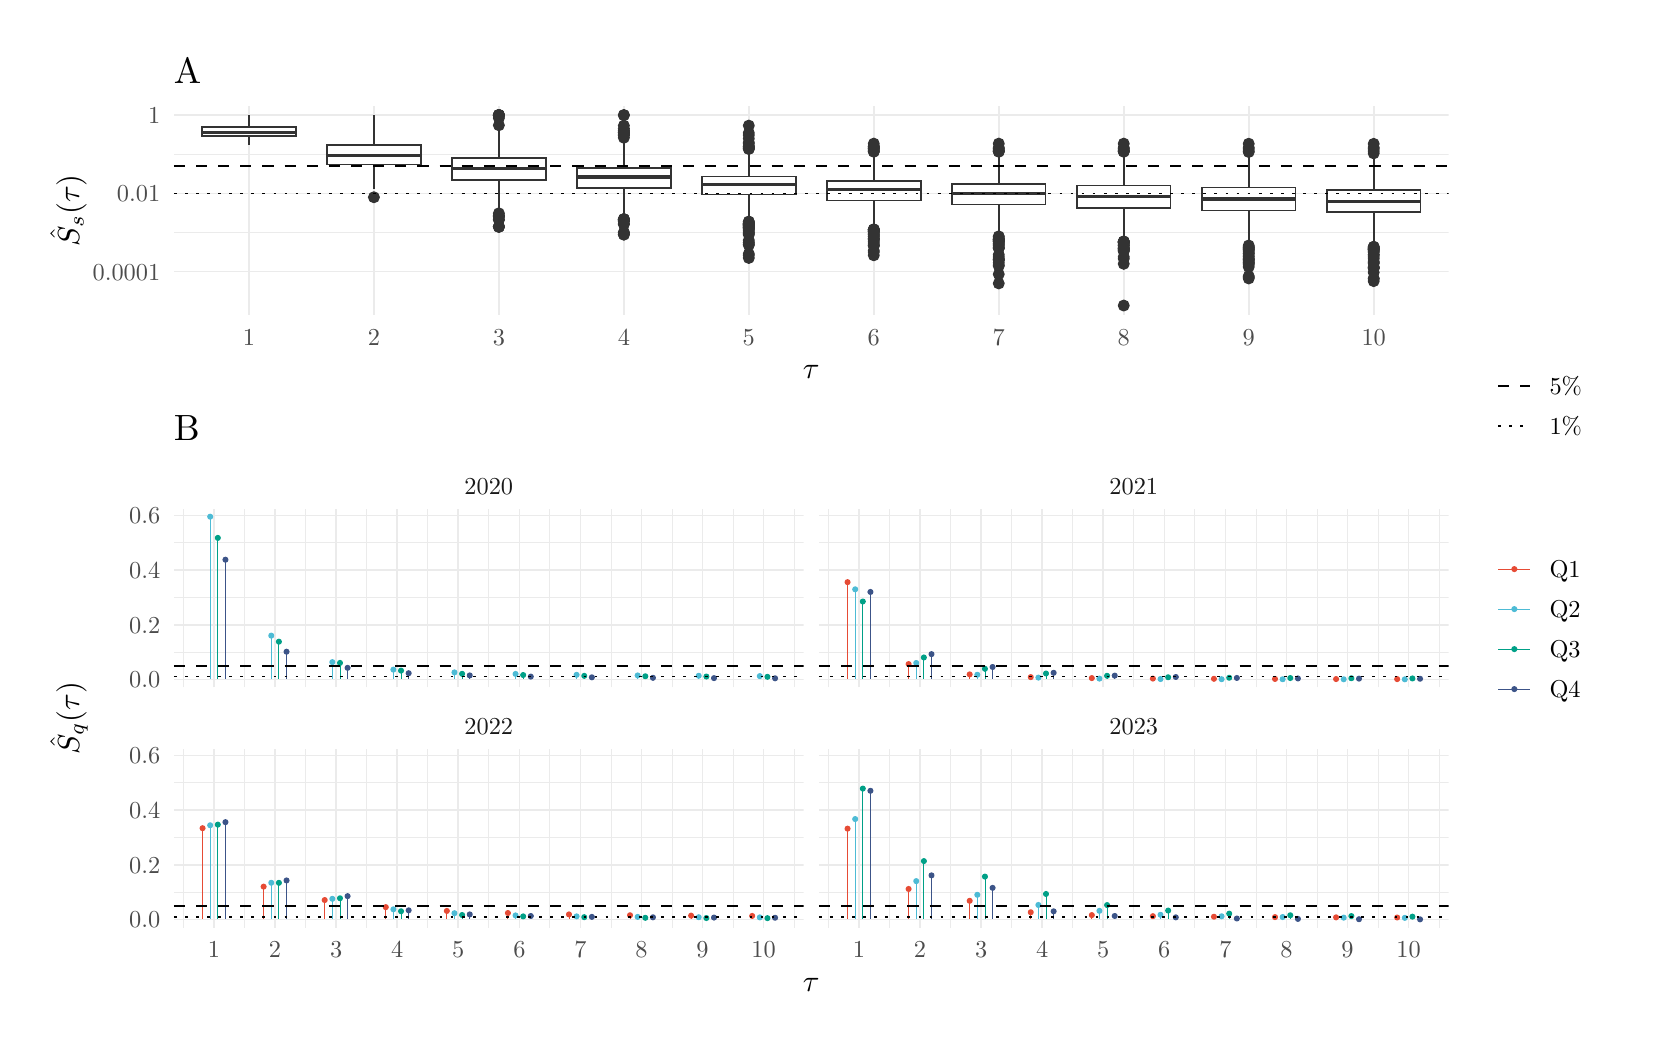
\begin{tikzpicture}[x=1pt,y=1pt]
\definecolor{fillColor}{RGB}{255,255,255}
\path[use as bounding box,fill=fillColor,fill opacity=0.00] (0,0) rectangle (578.16,361.35);
\begin{scope}
\path[clip] ( 52.85,257.50) rectangle (513.48,333.19);
\definecolor{drawColor}{gray}{0.92}

\path[draw=drawColor,line width= 0.3pt,line join=round] ( 52.85,315.61) --
	(513.48,315.61);

\path[draw=drawColor,line width= 0.3pt,line join=round] ( 52.85,287.33) --
	(513.48,287.33);

\path[draw=drawColor,line width= 0.6pt,line join=round] ( 52.85,329.75) --
	(513.48,329.75);

\path[draw=drawColor,line width= 0.6pt,line join=round] ( 52.85,301.47) --
	(513.48,301.47);

\path[draw=drawColor,line width= 0.6pt,line join=round] ( 52.85,273.19) --
	(513.48,273.19);

\path[draw=drawColor,line width= 0.6pt,line join=round] ( 79.95,257.50) --
	( 79.95,333.19);

\path[draw=drawColor,line width= 0.6pt,line join=round] (125.11,257.50) --
	(125.11,333.19);

\path[draw=drawColor,line width= 0.6pt,line join=round] (170.27,257.50) --
	(170.27,333.19);

\path[draw=drawColor,line width= 0.6pt,line join=round] (215.43,257.50) --
	(215.43,333.19);

\path[draw=drawColor,line width= 0.6pt,line join=round] (260.58,257.50) --
	(260.58,333.19);

\path[draw=drawColor,line width= 0.6pt,line join=round] (305.74,257.50) --
	(305.74,333.19);

\path[draw=drawColor,line width= 0.6pt,line join=round] (350.90,257.50) --
	(350.90,333.19);

\path[draw=drawColor,line width= 0.6pt,line join=round] (396.06,257.50) --
	(396.06,333.19);

\path[draw=drawColor,line width= 0.6pt,line join=round] (441.22,257.50) --
	(441.22,333.19);

\path[draw=drawColor,line width= 0.6pt,line join=round] (486.38,257.50) --
	(486.38,333.19);
\definecolor{drawColor}{gray}{0.20}

\path[draw=drawColor,line width= 0.6pt,line join=round] ( 79.95,325.40) -- ( 79.95,329.75);

\path[draw=drawColor,line width= 0.6pt,line join=round] ( 79.95,322.27) -- ( 79.95,319.12);
\definecolor{fillColor}{RGB}{255,255,255}

\path[draw=drawColor,line width= 0.6pt,fill=fillColor] ( 63.01,325.40) --
	( 63.01,322.27) --
	( 96.88,322.27) --
	( 96.88,325.40) --
	( 63.01,325.40) --
	cycle;

\path[draw=drawColor,line width= 1.1pt] ( 63.01,323.63) -- ( 96.88,323.63);
\definecolor{fillColor}{gray}{0.20}

\path[draw=drawColor,line width= 0.4pt,line join=round,line cap=round,fill=fillColor] (125.11,300.07) circle (  1.96);

\path[draw=drawColor,line width= 0.6pt,line join=round] (125.11,319.05) -- (125.11,329.75);

\path[draw=drawColor,line width= 0.6pt,line join=round] (125.11,311.87) -- (125.11,303.04);
\definecolor{fillColor}{RGB}{255,255,255}

\path[draw=drawColor,line width= 0.6pt,fill=fillColor] (108.17,319.05) --
	(108.17,311.87) --
	(142.04,311.87) --
	(142.04,319.05) --
	(108.17,319.05) --
	cycle;

\path[draw=drawColor,line width= 1.1pt] (108.17,315.23) -- (142.04,315.23);
\definecolor{fillColor}{gray}{0.20}

\path[draw=drawColor,line width= 0.4pt,line join=round,line cap=round,fill=fillColor] (170.27,293.25) circle (  1.96);

\path[draw=drawColor,line width= 0.4pt,line join=round,line cap=round,fill=fillColor] (170.27,291.85) circle (  1.96);

\path[draw=drawColor,line width= 0.4pt,line join=round,line cap=round,fill=fillColor] (170.27,289.53) circle (  1.96);

\path[draw=drawColor,line width= 0.4pt,line join=round,line cap=round,fill=fillColor] (170.27,289.45) circle (  1.96);

\path[draw=drawColor,line width= 0.4pt,line join=round,line cap=round,fill=fillColor] (170.27,293.33) circle (  1.96);

\path[draw=drawColor,line width= 0.4pt,line join=round,line cap=round,fill=fillColor] (170.27,289.36) circle (  1.96);

\path[draw=drawColor,line width= 0.4pt,line join=round,line cap=round,fill=fillColor] (170.27,294.26) circle (  1.96);

\path[draw=drawColor,line width= 0.4pt,line join=round,line cap=round,fill=fillColor] (170.27,293.01) circle (  1.96);

\path[draw=drawColor,line width= 0.4pt,line join=round,line cap=round,fill=fillColor] (170.27,293.38) circle (  1.96);

\path[draw=drawColor,line width= 0.4pt,line join=round,line cap=round,fill=fillColor] (170.27,289.39) circle (  1.96);

\path[draw=drawColor,line width= 0.4pt,line join=round,line cap=round,fill=fillColor] (170.27,292.10) circle (  1.96);

\path[draw=drawColor,line width= 0.4pt,line join=round,line cap=round,fill=fillColor] (170.27,328.67) circle (  1.96);

\path[draw=drawColor,line width= 0.4pt,line join=round,line cap=round,fill=fillColor] (170.27,329.75) circle (  1.96);

\path[draw=drawColor,line width= 0.4pt,line join=round,line cap=round,fill=fillColor] (170.27,329.74) circle (  1.96);

\path[draw=drawColor,line width= 0.4pt,line join=round,line cap=round,fill=fillColor] (170.27,326.09) circle (  1.96);

\path[draw=drawColor,line width= 0.4pt,line join=round,line cap=round,fill=fillColor] (170.27,329.75) circle (  1.96);

\path[draw=drawColor,line width= 0.4pt,line join=round,line cap=round,fill=fillColor] (170.27,329.75) circle (  1.96);

\path[draw=drawColor,line width= 0.4pt,line join=round,line cap=round,fill=fillColor] (170.27,329.75) circle (  1.96);

\path[draw=drawColor,line width= 0.4pt,line join=round,line cap=round,fill=fillColor] (170.27,329.75) circle (  1.96);

\path[draw=drawColor,line width= 0.4pt,line join=round,line cap=round,fill=fillColor] (170.27,329.75) circle (  1.96);

\path[draw=drawColor,line width= 0.4pt,line join=round,line cap=round,fill=fillColor] (170.27,329.75) circle (  1.96);

\path[draw=drawColor,line width= 0.6pt,line join=round] (170.27,314.22) -- (170.27,325.96);

\path[draw=drawColor,line width= 0.6pt,line join=round] (170.27,306.33) -- (170.27,294.51);
\definecolor{fillColor}{RGB}{255,255,255}

\path[draw=drawColor,line width= 0.6pt,fill=fillColor] (153.33,314.22) --
	(153.33,306.33) --
	(187.20,306.33) --
	(187.20,314.22) --
	(153.33,314.22) --
	cycle;

\path[draw=drawColor,line width= 1.1pt] (153.33,310.34) -- (187.20,310.34);
\definecolor{fillColor}{gray}{0.20}

\path[draw=drawColor,line width= 0.4pt,line join=round,line cap=round,fill=fillColor] (215.43,292.12) circle (  1.96);

\path[draw=drawColor,line width= 0.4pt,line join=round,line cap=round,fill=fillColor] (215.43,290.30) circle (  1.96);

\path[draw=drawColor,line width= 0.4pt,line join=round,line cap=round,fill=fillColor] (215.43,291.56) circle (  1.96);

\path[draw=drawColor,line width= 0.4pt,line join=round,line cap=round,fill=fillColor] (215.43,286.64) circle (  1.96);

\path[draw=drawColor,line width= 0.4pt,line join=round,line cap=round,fill=fillColor] (215.43,291.29) circle (  1.96);

\path[draw=drawColor,line width= 0.4pt,line join=round,line cap=round,fill=fillColor] (215.43,291.69) circle (  1.96);

\path[draw=drawColor,line width= 0.4pt,line join=round,line cap=round,fill=fillColor] (215.43,292.19) circle (  1.96);

\path[draw=drawColor,line width= 0.4pt,line join=round,line cap=round,fill=fillColor] (215.43,292.06) circle (  1.96);

\path[draw=drawColor,line width= 0.4pt,line join=round,line cap=round,fill=fillColor] (215.43,290.45) circle (  1.96);

\path[draw=drawColor,line width= 0.4pt,line join=round,line cap=round,fill=fillColor] (215.43,287.43) circle (  1.96);

\path[draw=drawColor,line width= 0.4pt,line join=round,line cap=round,fill=fillColor] (215.43,292.12) circle (  1.96);

\path[draw=drawColor,line width= 0.4pt,line join=round,line cap=round,fill=fillColor] (215.43,287.21) circle (  1.96);

\path[draw=drawColor,line width= 0.4pt,line join=round,line cap=round,fill=fillColor] (215.43,286.55) circle (  1.96);

\path[draw=drawColor,line width= 0.4pt,line join=round,line cap=round,fill=fillColor] (215.43,324.32) circle (  1.96);

\path[draw=drawColor,line width= 0.4pt,line join=round,line cap=round,fill=fillColor] (215.43,322.51) circle (  1.96);

\path[draw=drawColor,line width= 0.4pt,line join=round,line cap=round,fill=fillColor] (215.43,323.57) circle (  1.96);

\path[draw=drawColor,line width= 0.4pt,line join=round,line cap=round,fill=fillColor] (215.43,322.87) circle (  1.96);

\path[draw=drawColor,line width= 0.4pt,line join=round,line cap=round,fill=fillColor] (215.43,322.48) circle (  1.96);

\path[draw=drawColor,line width= 0.4pt,line join=round,line cap=round,fill=fillColor] (215.43,329.75) circle (  1.96);

\path[draw=drawColor,line width= 0.4pt,line join=round,line cap=round,fill=fillColor] (215.43,323.40) circle (  1.96);

\path[draw=drawColor,line width= 0.4pt,line join=round,line cap=round,fill=fillColor] (215.43,291.99) circle (  1.96);

\path[draw=drawColor,line width= 0.4pt,line join=round,line cap=round,fill=fillColor] (215.43,321.58) circle (  1.96);

\path[draw=drawColor,line width= 0.4pt,line join=round,line cap=round,fill=fillColor] (215.43,324.01) circle (  1.96);

\path[draw=drawColor,line width= 0.4pt,line join=round,line cap=round,fill=fillColor] (215.43,325.96) circle (  1.96);

\path[draw=drawColor,line width= 0.4pt,line join=round,line cap=round,fill=fillColor] (215.43,329.75) circle (  1.96);

\path[draw=drawColor,line width= 0.4pt,line join=round,line cap=round,fill=fillColor] (215.43,323.34) circle (  1.96);

\path[draw=drawColor,line width= 0.4pt,line join=round,line cap=round,fill=fillColor] (215.43,324.90) circle (  1.96);

\path[draw=drawColor,line width= 0.6pt,line join=round] (215.43,310.64) -- (215.43,321.53);

\path[draw=drawColor,line width= 0.6pt,line join=round] (215.43,303.37) -- (215.43,292.64);
\definecolor{fillColor}{RGB}{255,255,255}

\path[draw=drawColor,line width= 0.6pt,fill=fillColor] (198.49,310.64) --
	(198.49,303.37) --
	(232.36,303.37) --
	(232.36,310.64) --
	(198.49,310.64) --
	cycle;

\path[draw=drawColor,line width= 1.1pt] (198.49,307.38) -- (232.36,307.38);
\definecolor{fillColor}{gray}{0.20}

\path[draw=drawColor,line width= 0.4pt,line join=round,line cap=round,fill=fillColor] (260.58,287.59) circle (  1.96);

\path[draw=drawColor,line width= 0.4pt,line join=round,line cap=round,fill=fillColor] (260.58,289.63) circle (  1.96);

\path[draw=drawColor,line width= 0.4pt,line join=round,line cap=round,fill=fillColor] (260.58,289.73) circle (  1.96);

\path[draw=drawColor,line width= 0.4pt,line join=round,line cap=round,fill=fillColor] (260.58,290.30) circle (  1.96);

\path[draw=drawColor,line width= 0.4pt,line join=round,line cap=round,fill=fillColor] (260.58,319.45) circle (  1.96);

\path[draw=drawColor,line width= 0.4pt,line join=round,line cap=round,fill=fillColor] (260.58,318.33) circle (  1.96);

\path[draw=drawColor,line width= 0.4pt,line join=round,line cap=round,fill=fillColor] (260.58,291.19) circle (  1.96);

\path[draw=drawColor,line width= 0.4pt,line join=round,line cap=round,fill=fillColor] (260.58,290.59) circle (  1.96);

\path[draw=drawColor,line width= 0.4pt,line join=round,line cap=round,fill=fillColor] (260.58,289.12) circle (  1.96);

\path[draw=drawColor,line width= 0.4pt,line join=round,line cap=round,fill=fillColor] (260.58,288.99) circle (  1.96);

\path[draw=drawColor,line width= 0.4pt,line join=round,line cap=round,fill=fillColor] (260.58,290.31) circle (  1.96);

\path[draw=drawColor,line width= 0.4pt,line join=round,line cap=round,fill=fillColor] (260.58,278.13) circle (  1.96);

\path[draw=drawColor,line width= 0.4pt,line join=round,line cap=round,fill=fillColor] (260.58,291.29) circle (  1.96);

\path[draw=drawColor,line width= 0.4pt,line join=round,line cap=round,fill=fillColor] (260.58,279.09) circle (  1.96);

\path[draw=drawColor,line width= 0.4pt,line join=round,line cap=round,fill=fillColor] (260.58,290.02) circle (  1.96);

\path[draw=drawColor,line width= 0.4pt,line join=round,line cap=round,fill=fillColor] (260.58,289.81) circle (  1.96);

\path[draw=drawColor,line width= 0.4pt,line join=round,line cap=round,fill=fillColor] (260.58,282.96) circle (  1.96);

\path[draw=drawColor,line width= 0.4pt,line join=round,line cap=round,fill=fillColor] (260.58,287.18) circle (  1.96);

\path[draw=drawColor,line width= 0.4pt,line join=round,line cap=round,fill=fillColor] (260.58,279.65) circle (  1.96);

\path[draw=drawColor,line width= 0.4pt,line join=round,line cap=round,fill=fillColor] (260.58,289.56) circle (  1.96);

\path[draw=drawColor,line width= 0.4pt,line join=round,line cap=round,fill=fillColor] (260.58,288.57) circle (  1.96);

\path[draw=drawColor,line width= 0.4pt,line join=round,line cap=round,fill=fillColor] (260.58,284.53) circle (  1.96);

\path[draw=drawColor,line width= 0.4pt,line join=round,line cap=round,fill=fillColor] (260.58,282.83) circle (  1.96);

\path[draw=drawColor,line width= 0.4pt,line join=round,line cap=round,fill=fillColor] (260.58,283.78) circle (  1.96);

\path[draw=drawColor,line width= 0.4pt,line join=round,line cap=round,fill=fillColor] (260.58,286.96) circle (  1.96);

\path[draw=drawColor,line width= 0.4pt,line join=round,line cap=round,fill=fillColor] (260.58,288.13) circle (  1.96);

\path[draw=drawColor,line width= 0.4pt,line join=round,line cap=round,fill=fillColor] (260.58,283.57) circle (  1.96);

\path[draw=drawColor,line width= 0.4pt,line join=round,line cap=round,fill=fillColor] (260.58,289.17) circle (  1.96);

\path[draw=drawColor,line width= 0.4pt,line join=round,line cap=round,fill=fillColor] (260.58,289.09) circle (  1.96);

\path[draw=drawColor,line width= 0.4pt,line join=round,line cap=round,fill=fillColor] (260.58,290.57) circle (  1.96);

\path[draw=drawColor,line width= 0.4pt,line join=round,line cap=round,fill=fillColor] (260.58,286.52) circle (  1.96);

\path[draw=drawColor,line width= 0.4pt,line join=round,line cap=round,fill=fillColor] (260.58,290.52) circle (  1.96);

\path[draw=drawColor,line width= 0.4pt,line join=round,line cap=round,fill=fillColor] (260.58,288.74) circle (  1.96);

\path[draw=drawColor,line width= 0.4pt,line join=round,line cap=round,fill=fillColor] (260.58,290.05) circle (  1.96);

\path[draw=drawColor,line width= 0.4pt,line join=round,line cap=round,fill=fillColor] (260.58,290.71) circle (  1.96);

\path[draw=drawColor,line width= 0.4pt,line join=round,line cap=round,fill=fillColor] (260.58,318.58) circle (  1.96);

\path[draw=drawColor,line width= 0.4pt,line join=round,line cap=round,fill=fillColor] (260.58,322.48) circle (  1.96);

\path[draw=drawColor,line width= 0.4pt,line join=round,line cap=round,fill=fillColor] (260.58,321.26) circle (  1.96);

\path[draw=drawColor,line width= 0.4pt,line join=round,line cap=round,fill=fillColor] (260.58,290.22) circle (  1.96);

\path[draw=drawColor,line width= 0.4pt,line join=round,line cap=round,fill=fillColor] (260.58,319.87) circle (  1.96);

\path[draw=drawColor,line width= 0.4pt,line join=round,line cap=round,fill=fillColor] (260.58,317.52) circle (  1.96);

\path[draw=drawColor,line width= 0.4pt,line join=round,line cap=round,fill=fillColor] (260.58,317.59) circle (  1.96);

\path[draw=drawColor,line width= 0.4pt,line join=round,line cap=round,fill=fillColor] (260.58,318.17) circle (  1.96);

\path[draw=drawColor,line width= 0.4pt,line join=round,line cap=round,fill=fillColor] (260.58,325.96) circle (  1.96);

\path[draw=drawColor,line width= 0.4pt,line join=round,line cap=round,fill=fillColor] (260.58,317.79) circle (  1.96);

\path[draw=drawColor,line width= 0.4pt,line join=round,line cap=round,fill=fillColor] (260.58,323.34) circle (  1.96);

\path[draw=drawColor,line width= 0.6pt,line join=round] (260.58,307.60) -- (260.58,316.86);

\path[draw=drawColor,line width= 0.6pt,line join=round] (260.58,301.09) -- (260.58,291.43);
\definecolor{fillColor}{RGB}{255,255,255}

\path[draw=drawColor,line width= 0.6pt,fill=fillColor] (243.65,307.60) --
	(243.65,301.09) --
	(277.52,301.09) --
	(277.52,307.60) --
	(243.65,307.60) --
	cycle;

\path[draw=drawColor,line width= 1.1pt] (243.65,304.55) -- (277.52,304.55);
\definecolor{fillColor}{gray}{0.20}

\path[draw=drawColor,line width= 0.4pt,line join=round,line cap=round,fill=fillColor] (305.74,319.45) circle (  1.96);

\path[draw=drawColor,line width= 0.4pt,line join=round,line cap=round,fill=fillColor] (305.74,318.33) circle (  1.96);

\path[draw=drawColor,line width= 0.4pt,line join=round,line cap=round,fill=fillColor] (305.74,316.51) circle (  1.96);

\path[draw=drawColor,line width= 0.4pt,line join=round,line cap=round,fill=fillColor] (305.74,284.69) circle (  1.96);

\path[draw=drawColor,line width= 0.4pt,line join=round,line cap=round,fill=fillColor] (305.74,287.86) circle (  1.96);

\path[draw=drawColor,line width= 0.4pt,line join=round,line cap=round,fill=fillColor] (305.74,282.68) circle (  1.96);

\path[draw=drawColor,line width= 0.4pt,line join=round,line cap=round,fill=fillColor] (305.74,285.01) circle (  1.96);

\path[draw=drawColor,line width= 0.4pt,line join=round,line cap=round,fill=fillColor] (305.74,287.08) circle (  1.96);

\path[draw=drawColor,line width= 0.4pt,line join=round,line cap=round,fill=fillColor] (305.74,287.87) circle (  1.96);

\path[draw=drawColor,line width= 0.4pt,line join=round,line cap=round,fill=fillColor] (305.74,285.25) circle (  1.96);

\path[draw=drawColor,line width= 0.4pt,line join=round,line cap=round,fill=fillColor] (305.74,286.69) circle (  1.96);

\path[draw=drawColor,line width= 0.4pt,line join=round,line cap=round,fill=fillColor] (305.74,280.79) circle (  1.96);

\path[draw=drawColor,line width= 0.4pt,line join=round,line cap=round,fill=fillColor] (305.74,285.93) circle (  1.96);

\path[draw=drawColor,line width= 0.4pt,line join=round,line cap=round,fill=fillColor] (305.74,288.38) circle (  1.96);

\path[draw=drawColor,line width= 0.4pt,line join=round,line cap=round,fill=fillColor] (305.74,282.80) circle (  1.96);

\path[draw=drawColor,line width= 0.4pt,line join=round,line cap=round,fill=fillColor] (305.74,287.69) circle (  1.96);

\path[draw=drawColor,line width= 0.4pt,line join=round,line cap=round,fill=fillColor] (305.74,285.93) circle (  1.96);

\path[draw=drawColor,line width= 0.4pt,line join=round,line cap=round,fill=fillColor] (305.74,285.03) circle (  1.96);

\path[draw=drawColor,line width= 0.4pt,line join=round,line cap=round,fill=fillColor] (305.74,282.46) circle (  1.96);

\path[draw=drawColor,line width= 0.4pt,line join=round,line cap=round,fill=fillColor] (305.74,288.47) circle (  1.96);

\path[draw=drawColor,line width= 0.4pt,line join=round,line cap=round,fill=fillColor] (305.74,279.09) circle (  1.96);

\path[draw=drawColor,line width= 0.4pt,line join=round,line cap=round,fill=fillColor] (305.74,288.32) circle (  1.96);

\path[draw=drawColor,line width= 0.4pt,line join=round,line cap=round,fill=fillColor] (305.74,287.65) circle (  1.96);

\path[draw=drawColor,line width= 0.4pt,line join=round,line cap=round,fill=fillColor] (305.74,286.52) circle (  1.96);

\path[draw=drawColor,line width= 0.4pt,line join=round,line cap=round,fill=fillColor] (305.74,284.08) circle (  1.96);

\path[draw=drawColor,line width= 0.4pt,line join=round,line cap=round,fill=fillColor] (305.74,283.51) circle (  1.96);

\path[draw=drawColor,line width= 0.4pt,line join=round,line cap=round,fill=fillColor] (305.74,280.24) circle (  1.96);

\path[draw=drawColor,line width= 0.4pt,line join=round,line cap=round,fill=fillColor] (305.74,288.32) circle (  1.96);

\path[draw=drawColor,line width= 0.4pt,line join=round,line cap=round,fill=fillColor] (305.74,288.36) circle (  1.96);

\path[draw=drawColor,line width= 0.4pt,line join=round,line cap=round,fill=fillColor] (305.74,316.68) circle (  1.96);

\path[draw=drawColor,line width= 0.4pt,line join=round,line cap=round,fill=fillColor] (305.74,316.86) circle (  1.96);

\path[draw=drawColor,line width= 0.4pt,line join=round,line cap=round,fill=fillColor] (305.74,318.50) circle (  1.96);

\path[draw=drawColor,line width= 0.4pt,line join=round,line cap=round,fill=fillColor] (305.74,317.52) circle (  1.96);

\path[draw=drawColor,line width= 0.4pt,line join=round,line cap=round,fill=fillColor] (305.74,317.59) circle (  1.96);

\path[draw=drawColor,line width= 0.4pt,line join=round,line cap=round,fill=fillColor] (305.74,318.17) circle (  1.96);

\path[draw=drawColor,line width= 0.4pt,line join=round,line cap=round,fill=fillColor] (305.74,317.79) circle (  1.96);

\path[draw=drawColor,line width= 0.6pt,line join=round] (305.74,305.94) -- (305.74,315.23);

\path[draw=drawColor,line width= 0.6pt,line join=round] (305.74,298.95) -- (305.74,288.68);
\definecolor{fillColor}{RGB}{255,255,255}

\path[draw=drawColor,line width= 0.6pt,fill=fillColor] (288.81,305.94) --
	(288.81,298.95) --
	(322.68,298.95) --
	(322.68,305.94) --
	(288.81,305.94) --
	cycle;

\path[draw=drawColor,line width= 1.1pt] (288.81,302.75) -- (322.68,302.75);
\definecolor{fillColor}{gray}{0.20}

\path[draw=drawColor,line width= 0.4pt,line join=round,line cap=round,fill=fillColor] (350.90,319.45) circle (  1.96);

\path[draw=drawColor,line width= 0.4pt,line join=round,line cap=round,fill=fillColor] (350.90,318.04) circle (  1.96);

\path[draw=drawColor,line width= 0.4pt,line join=round,line cap=round,fill=fillColor] (350.90,316.51) circle (  1.96);

\path[draw=drawColor,line width= 0.4pt,line join=round,line cap=round,fill=fillColor] (350.90,284.69) circle (  1.96);

\path[draw=drawColor,line width= 0.4pt,line join=round,line cap=round,fill=fillColor] (350.90,277.55) circle (  1.96);

\path[draw=drawColor,line width= 0.4pt,line join=round,line cap=round,fill=fillColor] (350.90,284.97) circle (  1.96);

\path[draw=drawColor,line width= 0.4pt,line join=round,line cap=round,fill=fillColor] (350.90,281.73) circle (  1.96);

\path[draw=drawColor,line width= 0.4pt,line join=round,line cap=round,fill=fillColor] (350.90,279.31) circle (  1.96);

\path[draw=drawColor,line width= 0.4pt,line join=round,line cap=round,fill=fillColor] (350.90,284.73) circle (  1.96);

\path[draw=drawColor,line width= 0.4pt,line join=round,line cap=round,fill=fillColor] (350.90,284.15) circle (  1.96);

\path[draw=drawColor,line width= 0.4pt,line join=round,line cap=round,fill=fillColor] (350.90,282.80) circle (  1.96);

\path[draw=drawColor,line width= 0.4pt,line join=round,line cap=round,fill=fillColor] (350.90,284.37) circle (  1.96);

\path[draw=drawColor,line width= 0.4pt,line join=round,line cap=round,fill=fillColor] (350.90,285.01) circle (  1.96);

\path[draw=drawColor,line width= 0.4pt,line join=round,line cap=round,fill=fillColor] (350.90,268.93) circle (  1.96);

\path[draw=drawColor,line width= 0.4pt,line join=round,line cap=round,fill=fillColor] (350.90,275.57) circle (  1.96);

\path[draw=drawColor,line width= 0.4pt,line join=round,line cap=round,fill=fillColor] (350.90,282.46) circle (  1.96);

\path[draw=drawColor,line width= 0.4pt,line join=round,line cap=round,fill=fillColor] (350.90,277.27) circle (  1.96);

\path[draw=drawColor,line width= 0.4pt,line join=round,line cap=round,fill=fillColor] (350.90,272.26) circle (  1.96);

\path[draw=drawColor,line width= 0.4pt,line join=round,line cap=round,fill=fillColor] (350.90,276.44) circle (  1.96);

\path[draw=drawColor,line width= 0.4pt,line join=round,line cap=round,fill=fillColor] (350.90,278.50) circle (  1.96);

\path[draw=drawColor,line width= 0.4pt,line join=round,line cap=round,fill=fillColor] (350.90,284.06) circle (  1.96);

\path[draw=drawColor,line width= 0.4pt,line join=round,line cap=round,fill=fillColor] (350.90,277.78) circle (  1.96);

\path[draw=drawColor,line width= 0.4pt,line join=round,line cap=round,fill=fillColor] (350.90,284.08) circle (  1.96);

\path[draw=drawColor,line width= 0.4pt,line join=round,line cap=round,fill=fillColor] (350.90,283.19) circle (  1.96);

\path[draw=drawColor,line width= 0.4pt,line join=round,line cap=round,fill=fillColor] (350.90,277.55) circle (  1.96);

\path[draw=drawColor,line width= 0.4pt,line join=round,line cap=round,fill=fillColor] (350.90,281.71) circle (  1.96);

\path[draw=drawColor,line width= 0.4pt,line join=round,line cap=round,fill=fillColor] (350.90,275.26) circle (  1.96);

\path[draw=drawColor,line width= 0.4pt,line join=round,line cap=round,fill=fillColor] (350.90,284.71) circle (  1.96);

\path[draw=drawColor,line width= 0.4pt,line join=round,line cap=round,fill=fillColor] (350.90,283.41) circle (  1.96);

\path[draw=drawColor,line width= 0.4pt,line join=round,line cap=round,fill=fillColor] (350.90,285.94) circle (  1.96);

\path[draw=drawColor,line width= 0.4pt,line join=round,line cap=round,fill=fillColor] (350.90,281.71) circle (  1.96);

\path[draw=drawColor,line width= 0.4pt,line join=round,line cap=round,fill=fillColor] (350.90,316.68) circle (  1.96);

\path[draw=drawColor,line width= 0.4pt,line join=round,line cap=round,fill=fillColor] (350.90,316.86) circle (  1.96);

\path[draw=drawColor,line width= 0.4pt,line join=round,line cap=round,fill=fillColor] (350.90,316.73) circle (  1.96);

\path[draw=drawColor,line width= 0.4pt,line join=round,line cap=round,fill=fillColor] (350.90,317.52) circle (  1.96);

\path[draw=drawColor,line width= 0.4pt,line join=round,line cap=round,fill=fillColor] (350.90,317.59) circle (  1.96);

\path[draw=drawColor,line width= 0.4pt,line join=round,line cap=round,fill=fillColor] (350.90,285.70) circle (  1.96);

\path[draw=drawColor,line width= 0.6pt,line join=round] (350.90,304.88) -- (350.90,314.67);

\path[draw=drawColor,line width= 0.6pt,line join=round] (350.90,297.39) -- (350.90,286.41);
\definecolor{fillColor}{RGB}{255,255,255}

\path[draw=drawColor,line width= 0.6pt,fill=fillColor] (333.97,304.88) --
	(333.97,297.39) --
	(367.84,297.39) --
	(367.84,304.88) --
	(333.97,304.88) --
	cycle;

\path[draw=drawColor,line width= 1.1pt] (333.97,301.29) -- (367.84,301.29);
\definecolor{fillColor}{gray}{0.20}

\path[draw=drawColor,line width= 0.4pt,line join=round,line cap=round,fill=fillColor] (396.06,319.45) circle (  1.96);

\path[draw=drawColor,line width= 0.4pt,line join=round,line cap=round,fill=fillColor] (396.06,318.04) circle (  1.96);

\path[draw=drawColor,line width= 0.4pt,line join=round,line cap=round,fill=fillColor] (396.06,316.51) circle (  1.96);

\path[draw=drawColor,line width= 0.4pt,line join=round,line cap=round,fill=fillColor] (396.06,283.60) circle (  1.96);

\path[draw=drawColor,line width= 0.4pt,line join=round,line cap=round,fill=fillColor] (396.06,277.88) circle (  1.96);

\path[draw=drawColor,line width= 0.4pt,line join=round,line cap=round,fill=fillColor] (396.06,280.72) circle (  1.96);

\path[draw=drawColor,line width= 0.4pt,line join=round,line cap=round,fill=fillColor] (396.06,280.61) circle (  1.96);

\path[draw=drawColor,line width= 0.4pt,line join=round,line cap=round,fill=fillColor] (396.06,282.78) circle (  1.96);

\path[draw=drawColor,line width= 0.4pt,line join=round,line cap=round,fill=fillColor] (396.06,281.43) circle (  1.96);

\path[draw=drawColor,line width= 0.4pt,line join=round,line cap=round,fill=fillColor] (396.06,283.16) circle (  1.96);

\path[draw=drawColor,line width= 0.4pt,line join=round,line cap=round,fill=fillColor] (396.06,282.64) circle (  1.96);

\path[draw=drawColor,line width= 0.4pt,line join=round,line cap=round,fill=fillColor] (396.06,281.50) circle (  1.96);

\path[draw=drawColor,line width= 0.4pt,line join=round,line cap=round,fill=fillColor] (396.06,284.06) circle (  1.96);

\path[draw=drawColor,line width= 0.4pt,line join=round,line cap=round,fill=fillColor] (396.06,283.85) circle (  1.96);

\path[draw=drawColor,line width= 0.4pt,line join=round,line cap=round,fill=fillColor] (396.06,284.08) circle (  1.96);

\path[draw=drawColor,line width= 0.4pt,line join=round,line cap=round,fill=fillColor] (396.06,284.02) circle (  1.96);

\path[draw=drawColor,line width= 0.4pt,line join=round,line cap=round,fill=fillColor] (396.06,260.94) circle (  1.96);

\path[draw=drawColor,line width= 0.4pt,line join=round,line cap=round,fill=fillColor] (396.06,281.36) circle (  1.96);

\path[draw=drawColor,line width= 0.4pt,line join=round,line cap=round,fill=fillColor] (396.06,283.80) circle (  1.96);

\path[draw=drawColor,line width= 0.4pt,line join=round,line cap=round,fill=fillColor] (396.06,281.01) circle (  1.96);

\path[draw=drawColor,line width= 0.4pt,line join=round,line cap=round,fill=fillColor] (396.06,283.91) circle (  1.96);

\path[draw=drawColor,line width= 0.4pt,line join=round,line cap=round,fill=fillColor] (396.06,282.51) circle (  1.96);

\path[draw=drawColor,line width= 0.4pt,line join=round,line cap=round,fill=fillColor] (396.06,283.90) circle (  1.96);

\path[draw=drawColor,line width= 0.4pt,line join=round,line cap=round,fill=fillColor] (396.06,276.01) circle (  1.96);

\path[draw=drawColor,line width= 0.4pt,line join=round,line cap=round,fill=fillColor] (396.06,283.86) circle (  1.96);

\path[draw=drawColor,line width= 0.4pt,line join=round,line cap=round,fill=fillColor] (396.06,281.78) circle (  1.96);

\path[draw=drawColor,line width= 0.4pt,line join=round,line cap=round,fill=fillColor] (396.06,278.55) circle (  1.96);

\path[draw=drawColor,line width= 0.4pt,line join=round,line cap=round,fill=fillColor] (396.06,281.71) circle (  1.96);

\path[draw=drawColor,line width= 0.4pt,line join=round,line cap=round,fill=fillColor] (396.06,316.68) circle (  1.96);

\path[draw=drawColor,line width= 0.4pt,line join=round,line cap=round,fill=fillColor] (396.06,316.86) circle (  1.96);

\path[draw=drawColor,line width= 0.4pt,line join=round,line cap=round,fill=fillColor] (396.06,316.73) circle (  1.96);

\path[draw=drawColor,line width= 0.4pt,line join=round,line cap=round,fill=fillColor] (396.06,317.52) circle (  1.96);

\path[draw=drawColor,line width= 0.4pt,line join=round,line cap=round,fill=fillColor] (396.06,317.59) circle (  1.96);

\path[draw=drawColor,line width= 0.6pt,line join=round] (396.06,304.27) -- (396.06,314.67);

\path[draw=drawColor,line width= 0.6pt,line join=round] (396.06,296.21) -- (396.06,284.15);
\definecolor{fillColor}{RGB}{255,255,255}

\path[draw=drawColor,line width= 0.6pt,fill=fillColor] (379.13,304.27) --
	(379.13,296.21) --
	(413.00,296.21) --
	(413.00,304.27) --
	(379.13,304.27) --
	cycle;

\path[draw=drawColor,line width= 1.1pt] (379.13,300.18) -- (413.00,300.18);
\definecolor{fillColor}{gray}{0.20}

\path[draw=drawColor,line width= 0.4pt,line join=round,line cap=round,fill=fillColor] (441.22,319.41) circle (  1.96);

\path[draw=drawColor,line width= 0.4pt,line join=round,line cap=round,fill=fillColor] (441.22,318.04) circle (  1.96);

\path[draw=drawColor,line width= 0.4pt,line join=round,line cap=round,fill=fillColor] (441.22,316.42) circle (  1.96);

\path[draw=drawColor,line width= 0.4pt,line join=round,line cap=round,fill=fillColor] (441.22,276.68) circle (  1.96);

\path[draw=drawColor,line width= 0.4pt,line join=round,line cap=round,fill=fillColor] (441.22,276.42) circle (  1.96);

\path[draw=drawColor,line width= 0.4pt,line join=round,line cap=round,fill=fillColor] (441.22,274.90) circle (  1.96);

\path[draw=drawColor,line width= 0.4pt,line join=round,line cap=round,fill=fillColor] (441.22,270.73) circle (  1.96);

\path[draw=drawColor,line width= 0.4pt,line join=round,line cap=round,fill=fillColor] (441.22,275.70) circle (  1.96);

\path[draw=drawColor,line width= 0.4pt,line join=round,line cap=round,fill=fillColor] (441.22,282.10) circle (  1.96);

\path[draw=drawColor,line width= 0.4pt,line join=round,line cap=round,fill=fillColor] (441.22,281.14) circle (  1.96);

\path[draw=drawColor,line width= 0.4pt,line join=round,line cap=round,fill=fillColor] (441.22,277.87) circle (  1.96);

\path[draw=drawColor,line width= 0.4pt,line join=round,line cap=round,fill=fillColor] (441.22,277.17) circle (  1.96);

\path[draw=drawColor,line width= 0.4pt,line join=round,line cap=round,fill=fillColor] (441.22,282.64) circle (  1.96);

\path[draw=drawColor,line width= 0.4pt,line join=round,line cap=round,fill=fillColor] (441.22,280.40) circle (  1.96);

\path[draw=drawColor,line width= 0.4pt,line join=round,line cap=round,fill=fillColor] (441.22,276.18) circle (  1.96);

\path[draw=drawColor,line width= 0.4pt,line join=round,line cap=round,fill=fillColor] (441.22,281.38) circle (  1.96);

\path[draw=drawColor,line width= 0.4pt,line join=round,line cap=round,fill=fillColor] (441.22,282.02) circle (  1.96);

\path[draw=drawColor,line width= 0.4pt,line join=round,line cap=round,fill=fillColor] (441.22,278.89) circle (  1.96);

\path[draw=drawColor,line width= 0.4pt,line join=round,line cap=round,fill=fillColor] (441.22,281.01) circle (  1.96);

\path[draw=drawColor,line width= 0.4pt,line join=round,line cap=round,fill=fillColor] (441.22,277.69) circle (  1.96);

\path[draw=drawColor,line width= 0.4pt,line join=round,line cap=round,fill=fillColor] (441.22,279.64) circle (  1.96);

\path[draw=drawColor,line width= 0.4pt,line join=round,line cap=round,fill=fillColor] (441.22,271.18) circle (  1.96);

\path[draw=drawColor,line width= 0.4pt,line join=round,line cap=round,fill=fillColor] (441.22,279.83) circle (  1.96);

\path[draw=drawColor,line width= 0.4pt,line join=round,line cap=round,fill=fillColor] (441.22,271.58) circle (  1.96);

\path[draw=drawColor,line width= 0.4pt,line join=round,line cap=round,fill=fillColor] (441.22,277.52) circle (  1.96);

\path[draw=drawColor,line width= 0.4pt,line join=round,line cap=round,fill=fillColor] (441.22,278.55) circle (  1.96);

\path[draw=drawColor,line width= 0.4pt,line join=round,line cap=round,fill=fillColor] (441.22,281.71) circle (  1.96);

\path[draw=drawColor,line width= 0.4pt,line join=round,line cap=round,fill=fillColor] (441.22,316.73) circle (  1.96);

\path[draw=drawColor,line width= 0.4pt,line join=round,line cap=round,fill=fillColor] (441.22,317.52) circle (  1.96);

\path[draw=drawColor,line width= 0.6pt,line join=round] (441.22,303.58) -- (441.22,315.31);

\path[draw=drawColor,line width= 0.6pt,line join=round] (441.22,295.23) -- (441.22,282.91);
\definecolor{fillColor}{RGB}{255,255,255}

\path[draw=drawColor,line width= 0.6pt,fill=fillColor] (424.29,303.58) --
	(424.29,295.23) --
	(458.16,295.23) --
	(458.16,303.58) --
	(424.29,303.58) --
	cycle;

\path[draw=drawColor,line width= 1.1pt] (424.29,299.43) -- (458.16,299.43);
\definecolor{fillColor}{gray}{0.20}

\path[draw=drawColor,line width= 0.4pt,line join=round,line cap=round,fill=fillColor] (486.38,319.37) circle (  1.96);

\path[draw=drawColor,line width= 0.4pt,line join=round,line cap=round,fill=fillColor] (486.38,318.04) circle (  1.96);

\path[draw=drawColor,line width= 0.4pt,line join=round,line cap=round,fill=fillColor] (486.38,315.93) circle (  1.96);

\path[draw=drawColor,line width= 0.4pt,line join=round,line cap=round,fill=fillColor] (486.38,279.34) circle (  1.96);

\path[draw=drawColor,line width= 0.4pt,line join=round,line cap=round,fill=fillColor] (486.38,276.42) circle (  1.96);

\path[draw=drawColor,line width= 0.4pt,line join=round,line cap=round,fill=fillColor] (486.38,274.90) circle (  1.96);

\path[draw=drawColor,line width= 0.4pt,line join=round,line cap=round,fill=fillColor] (486.38,270.73) circle (  1.96);

\path[draw=drawColor,line width= 0.4pt,line join=round,line cap=round,fill=fillColor] (486.38,282.10) circle (  1.96);

\path[draw=drawColor,line width= 0.4pt,line join=round,line cap=round,fill=fillColor] (486.38,281.14) circle (  1.96);

\path[draw=drawColor,line width= 0.4pt,line join=round,line cap=round,fill=fillColor] (486.38,277.87) circle (  1.96);

\path[draw=drawColor,line width= 0.4pt,line join=round,line cap=round,fill=fillColor] (486.38,272.91) circle (  1.96);

\path[draw=drawColor,line width= 0.4pt,line join=round,line cap=round,fill=fillColor] (486.38,280.27) circle (  1.96);

\path[draw=drawColor,line width= 0.4pt,line join=round,line cap=round,fill=fillColor] (486.38,276.86) circle (  1.96);

\path[draw=drawColor,line width= 0.4pt,line join=round,line cap=round,fill=fillColor] (486.38,280.40) circle (  1.96);

\path[draw=drawColor,line width= 0.4pt,line join=round,line cap=round,fill=fillColor] (486.38,270.66) circle (  1.96);

\path[draw=drawColor,line width= 0.4pt,line join=round,line cap=round,fill=fillColor] (486.38,276.18) circle (  1.96);

\path[draw=drawColor,line width= 0.4pt,line join=round,line cap=round,fill=fillColor] (486.38,281.38) circle (  1.96);

\path[draw=drawColor,line width= 0.4pt,line join=round,line cap=round,fill=fillColor] (486.38,281.33) circle (  1.96);

\path[draw=drawColor,line width= 0.4pt,line join=round,line cap=round,fill=fillColor] (486.38,281.17) circle (  1.96);

\path[draw=drawColor,line width= 0.4pt,line join=round,line cap=round,fill=fillColor] (486.38,274.62) circle (  1.96);

\path[draw=drawColor,line width= 0.4pt,line join=round,line cap=round,fill=fillColor] (486.38,281.01) circle (  1.96);

\path[draw=drawColor,line width= 0.4pt,line join=round,line cap=round,fill=fillColor] (486.38,274.38) circle (  1.96);

\path[draw=drawColor,line width= 0.4pt,line join=round,line cap=round,fill=fillColor] (486.38,281.74) circle (  1.96);

\path[draw=drawColor,line width= 0.4pt,line join=round,line cap=round,fill=fillColor] (486.38,269.76) circle (  1.96);

\path[draw=drawColor,line width= 0.4pt,line join=round,line cap=round,fill=fillColor] (486.38,274.54) circle (  1.96);

\path[draw=drawColor,line width= 0.4pt,line join=round,line cap=round,fill=fillColor] (486.38,279.28) circle (  1.96);

\path[draw=drawColor,line width= 0.4pt,line join=round,line cap=round,fill=fillColor] (486.38,278.55) circle (  1.96);

\path[draw=drawColor,line width= 0.4pt,line join=round,line cap=round,fill=fillColor] (486.38,281.71) circle (  1.96);

\path[draw=drawColor,line width= 0.4pt,line join=round,line cap=round,fill=fillColor] (486.38,316.73) circle (  1.96);

\path[draw=drawColor,line width= 0.4pt,line join=round,line cap=round,fill=fillColor] (486.38,317.52) circle (  1.96);

\path[draw=drawColor,line width= 0.4pt,line join=round,line cap=round,fill=fillColor] (486.38,282.20) circle (  1.96);

\path[draw=drawColor,line width= 0.6pt,line join=round] (486.38,302.76) -- (486.38,314.67);

\path[draw=drawColor,line width= 0.6pt,line join=round] (486.38,294.63) -- (486.38,282.42);
\definecolor{fillColor}{RGB}{255,255,255}

\path[draw=drawColor,line width= 0.6pt,fill=fillColor] (469.45,302.76) --
	(469.45,294.63) --
	(503.31,294.63) --
	(503.31,302.76) --
	(469.45,302.76) --
	cycle;

\path[draw=drawColor,line width= 1.1pt] (469.45,298.65) -- (503.31,298.65);
\definecolor{drawColor}{RGB}{0,0,0}

\path[draw=drawColor,line width= 0.6pt,dash pattern=on 4pt off 4pt ,line join=round] ( 52.85,311.36) -- (513.48,311.36);

\path[draw=drawColor,line width= 0.6pt,dash pattern=on 1pt off 3pt ,line join=round] ( 52.85,301.47) -- (513.48,301.47);
\end{scope}
\begin{scope}
\path[clip] (  0.00,  0.00) rectangle (578.16,361.35);
\definecolor{drawColor}{gray}{0.30}

\node[text=drawColor,anchor=base east,inner sep=0pt, outer sep=0pt, scale=  0.88] at ( 47.90,326.72) {1};

\node[text=drawColor,anchor=base east,inner sep=0pt, outer sep=0pt, scale=  0.88] at ( 47.90,298.44) {0.01};

\node[text=drawColor,anchor=base east,inner sep=0pt, outer sep=0pt, scale=  0.88] at ( 47.90,270.16) {0.0001};
\end{scope}
\begin{scope}
\path[clip] (  0.00,  0.00) rectangle (578.16,361.35);
\definecolor{drawColor}{gray}{0.30}

\node[text=drawColor,anchor=base,inner sep=0pt, outer sep=0pt, scale=  0.88] at ( 79.95,246.48) {1};

\node[text=drawColor,anchor=base,inner sep=0pt, outer sep=0pt, scale=  0.88] at (125.11,246.48) {2};

\node[text=drawColor,anchor=base,inner sep=0pt, outer sep=0pt, scale=  0.88] at (170.27,246.48) {3};

\node[text=drawColor,anchor=base,inner sep=0pt, outer sep=0pt, scale=  0.88] at (215.43,246.48) {4};

\node[text=drawColor,anchor=base,inner sep=0pt, outer sep=0pt, scale=  0.88] at (260.58,246.48) {5};

\node[text=drawColor,anchor=base,inner sep=0pt, outer sep=0pt, scale=  0.88] at (305.74,246.48) {6};

\node[text=drawColor,anchor=base,inner sep=0pt, outer sep=0pt, scale=  0.88] at (350.90,246.48) {7};

\node[text=drawColor,anchor=base,inner sep=0pt, outer sep=0pt, scale=  0.88] at (396.06,246.48) {8};

\node[text=drawColor,anchor=base,inner sep=0pt, outer sep=0pt, scale=  0.88] at (441.22,246.48) {9};

\node[text=drawColor,anchor=base,inner sep=0pt, outer sep=0pt, scale=  0.88] at (486.38,246.48) {10};
\end{scope}
\begin{scope}
\path[clip] (  0.00,  0.00) rectangle (578.16,361.35);
\definecolor{drawColor}{RGB}{0,0,0}

\node[text=drawColor,anchor=base,inner sep=0pt, outer sep=0pt, scale=  1.10] at (283.16,234.45) {$\tau$};
\end{scope}
\begin{scope}
\path[clip] (  0.00,  0.00) rectangle (578.16,361.35);
\definecolor{drawColor}{RGB}{0,0,0}

\node[text=drawColor,rotate= 90.00,anchor=base,inner sep=0pt, outer sep=0pt, scale=  1.10] at ( 18.58,295.34) {$\hat S_{s}(\tau)$};
\end{scope}
\begin{scope}
\path[clip] (  0.00,  0.00) rectangle (578.16,361.35);
\definecolor{drawColor}{RGB}{0,0,0}

\node[text=drawColor,anchor=base west,inner sep=0pt, outer sep=0pt, scale=  1.32] at ( 52.85,341.26) {A};
\end{scope}
\begin{scope}
\path[clip] ( 52.85,122.92) rectangle (280.41,187.58);
\definecolor{drawColor}{gray}{0.92}

\path[draw=drawColor,line width= 0.3pt,line join=round] ( 52.85,135.73) --
	(280.41,135.73);

\path[draw=drawColor,line width= 0.3pt,line join=round] ( 52.85,155.46) --
	(280.41,155.46);

\path[draw=drawColor,line width= 0.3pt,line join=round] ( 52.85,175.20) --
	(280.41,175.20);

\path[draw=drawColor,line width= 0.3pt,line join=round] ( 56.30,122.92) --
	( 56.30,187.58);

\path[draw=drawColor,line width= 0.3pt,line join=round] ( 78.37,122.92) --
	( 78.37,187.58);

\path[draw=drawColor,line width= 0.3pt,line join=round] (100.43,122.92) --
	(100.43,187.58);

\path[draw=drawColor,line width= 0.3pt,line join=round] (122.50,122.92) --
	(122.50,187.58);

\path[draw=drawColor,line width= 0.3pt,line join=round] (144.57,122.92) --
	(144.57,187.58);

\path[draw=drawColor,line width= 0.3pt,line join=round] (166.63,122.92) --
	(166.63,187.58);

\path[draw=drawColor,line width= 0.3pt,line join=round] (188.70,122.92) --
	(188.70,187.58);

\path[draw=drawColor,line width= 0.3pt,line join=round] (210.77,122.92) --
	(210.77,187.58);

\path[draw=drawColor,line width= 0.3pt,line join=round] (232.83,122.92) --
	(232.83,187.58);

\path[draw=drawColor,line width= 0.3pt,line join=round] (254.90,122.92) --
	(254.90,187.58);

\path[draw=drawColor,line width= 0.3pt,line join=round] (276.97,122.92) --
	(276.97,187.58);

\path[draw=drawColor,line width= 0.6pt,line join=round] ( 52.85,125.86) --
	(280.41,125.86);

\path[draw=drawColor,line width= 0.6pt,line join=round] ( 52.85,145.60) --
	(280.41,145.60);

\path[draw=drawColor,line width= 0.6pt,line join=round] ( 52.85,165.33) --
	(280.41,165.33);

\path[draw=drawColor,line width= 0.6pt,line join=round] ( 52.85,185.07) --
	(280.41,185.07);

\path[draw=drawColor,line width= 0.6pt,line join=round] ( 67.33,122.92) --
	( 67.33,187.58);

\path[draw=drawColor,line width= 0.6pt,line join=round] ( 89.40,122.92) --
	( 89.40,187.58);

\path[draw=drawColor,line width= 0.6pt,line join=round] (111.47,122.92) --
	(111.47,187.58);

\path[draw=drawColor,line width= 0.6pt,line join=round] (133.53,122.92) --
	(133.53,187.58);

\path[draw=drawColor,line width= 0.6pt,line join=round] (155.60,122.92) --
	(155.60,187.58);

\path[draw=drawColor,line width= 0.6pt,line join=round] (177.67,122.92) --
	(177.67,187.58);

\path[draw=drawColor,line width= 0.6pt,line join=round] (199.73,122.92) --
	(199.73,187.58);

\path[draw=drawColor,line width= 0.6pt,line join=round] (221.80,122.92) --
	(221.80,187.58);

\path[draw=drawColor,line width= 0.6pt,line join=round] (243.87,122.92) --
	(243.87,187.58);

\path[draw=drawColor,line width= 0.6pt,line join=round] (265.93,122.92) --
	(265.93,187.58);
\definecolor{drawColor}{RGB}{77,187,213}
\definecolor{fillColor}{RGB}{77,187,213}

\path[draw=drawColor,line width= 0.4pt,line join=round,line cap=round,fill=fillColor] ( 65.95,184.64) circle (  0.89);

\path[draw=drawColor,line width= 0.4pt,line join=round,line cap=round,fill=fillColor] ( 88.02,141.66) circle (  0.89);

\path[draw=drawColor,line width= 0.4pt,line join=round,line cap=round,fill=fillColor] (110.09,132.09) circle (  0.89);

\path[draw=drawColor,line width= 0.4pt,line join=round,line cap=round,fill=fillColor] (132.15,129.38) circle (  0.89);

\path[draw=drawColor,line width= 0.4pt,line join=round,line cap=round,fill=fillColor] (154.22,128.38) circle (  0.89);

\path[draw=drawColor,line width= 0.4pt,line join=round,line cap=round,fill=fillColor] (176.29,127.82) circle (  0.89);

\path[draw=drawColor,line width= 0.4pt,line join=round,line cap=round,fill=fillColor] (198.35,127.50) circle (  0.89);

\path[draw=drawColor,line width= 0.4pt,line join=round,line cap=round,fill=fillColor] (220.42,127.28) circle (  0.89);

\path[draw=drawColor,line width= 0.4pt,line join=round,line cap=round,fill=fillColor] (242.49,127.16) circle (  0.89);

\path[draw=drawColor,line width= 0.4pt,line join=round,line cap=round,fill=fillColor] (264.55,127.03) circle (  0.89);
\definecolor{drawColor}{RGB}{0,160,135}
\definecolor{fillColor}{RGB}{0,160,135}

\path[draw=drawColor,line width= 0.4pt,line join=round,line cap=round,fill=fillColor] ( 68.71,176.98) circle (  0.89);

\path[draw=drawColor,line width= 0.4pt,line join=round,line cap=round,fill=fillColor] ( 90.78,139.48) circle (  0.89);

\path[draw=drawColor,line width= 0.4pt,line join=round,line cap=round,fill=fillColor] (112.85,131.80) circle (  0.89);

\path[draw=drawColor,line width= 0.4pt,line join=round,line cap=round,fill=fillColor] (134.91,129.01) circle (  0.89);

\path[draw=drawColor,line width= 0.4pt,line join=round,line cap=round,fill=fillColor] (156.98,127.86) circle (  0.89);

\path[draw=drawColor,line width= 0.4pt,line join=round,line cap=round,fill=fillColor] (179.05,127.43) circle (  0.89);

\path[draw=drawColor,line width= 0.4pt,line join=round,line cap=round,fill=fillColor] (201.11,127.13) circle (  0.89);

\path[draw=drawColor,line width= 0.4pt,line join=round,line cap=round,fill=fillColor] (223.18,126.98) circle (  0.89);

\path[draw=drawColor,line width= 0.4pt,line join=round,line cap=round,fill=fillColor] (245.25,126.88) circle (  0.89);

\path[draw=drawColor,line width= 0.4pt,line join=round,line cap=round,fill=fillColor] (267.31,126.78) circle (  0.89);
\definecolor{drawColor}{RGB}{60,84,136}
\definecolor{fillColor}{RGB}{60,84,136}

\path[draw=drawColor,line width= 0.4pt,line join=round,line cap=round,fill=fillColor] ( 71.47,169.10) circle (  0.89);

\path[draw=drawColor,line width= 0.4pt,line join=round,line cap=round,fill=fillColor] ( 93.54,135.85) circle (  0.89);

\path[draw=drawColor,line width= 0.4pt,line join=round,line cap=round,fill=fillColor] (115.60,130.02) circle (  0.89);

\path[draw=drawColor,line width= 0.4pt,line join=round,line cap=round,fill=fillColor] (137.67,128.08) circle (  0.89);

\path[draw=drawColor,line width= 0.4pt,line join=round,line cap=round,fill=fillColor] (159.74,127.28) circle (  0.89);

\path[draw=drawColor,line width= 0.4pt,line join=round,line cap=round,fill=fillColor] (181.80,126.85) circle (  0.89);

\path[draw=drawColor,line width= 0.4pt,line join=round,line cap=round,fill=fillColor] (203.87,126.60) circle (  0.89);

\path[draw=drawColor,line width= 0.4pt,line join=round,line cap=round,fill=fillColor] (225.94,126.42) circle (  0.89);

\path[draw=drawColor,line width= 0.4pt,line join=round,line cap=round,fill=fillColor] (248.00,126.31) circle (  0.89);

\path[draw=drawColor,line width= 0.4pt,line join=round,line cap=round,fill=fillColor] (270.07,126.25) circle (  0.89);
\definecolor{drawColor}{RGB}{77,187,213}

\path[draw=drawColor,line width= 0.3pt,line join=round] ( 65.95,184.64) -- ( 65.95,125.86);

\path[draw=drawColor,line width= 0.3pt,line join=round] ( 88.02,141.66) -- ( 88.02,125.86);

\path[draw=drawColor,line width= 0.3pt,line join=round] (110.09,132.09) -- (110.09,125.86);

\path[draw=drawColor,line width= 0.3pt,line join=round] (132.15,129.38) -- (132.15,125.86);

\path[draw=drawColor,line width= 0.3pt,line join=round] (154.22,128.38) -- (154.22,125.86);

\path[draw=drawColor,line width= 0.3pt,line join=round] (176.29,127.82) -- (176.29,125.86);

\path[draw=drawColor,line width= 0.3pt,line join=round] (198.35,127.50) -- (198.35,125.86);

\path[draw=drawColor,line width= 0.3pt,line join=round] (220.42,127.28) -- (220.42,125.86);

\path[draw=drawColor,line width= 0.3pt,line join=round] (242.49,127.16) -- (242.49,125.86);

\path[draw=drawColor,line width= 0.3pt,line join=round] (264.55,127.03) -- (264.55,125.86);
\definecolor{drawColor}{RGB}{0,160,135}

\path[draw=drawColor,line width= 0.3pt,line join=round] ( 68.71,176.98) -- ( 68.71,125.86);

\path[draw=drawColor,line width= 0.3pt,line join=round] ( 90.78,139.48) -- ( 90.78,125.86);

\path[draw=drawColor,line width= 0.3pt,line join=round] (112.85,131.80) -- (112.85,125.86);

\path[draw=drawColor,line width= 0.3pt,line join=round] (134.91,129.01) -- (134.91,125.86);

\path[draw=drawColor,line width= 0.3pt,line join=round] (156.98,127.86) -- (156.98,125.86);

\path[draw=drawColor,line width= 0.3pt,line join=round] (179.05,127.43) -- (179.05,125.86);

\path[draw=drawColor,line width= 0.3pt,line join=round] (201.11,127.13) -- (201.11,125.86);

\path[draw=drawColor,line width= 0.3pt,line join=round] (223.18,126.98) -- (223.18,125.86);

\path[draw=drawColor,line width= 0.3pt,line join=round] (245.25,126.88) -- (245.25,125.86);

\path[draw=drawColor,line width= 0.3pt,line join=round] (267.31,126.78) -- (267.31,125.86);
\definecolor{drawColor}{RGB}{60,84,136}

\path[draw=drawColor,line width= 0.3pt,line join=round] ( 71.47,169.10) -- ( 71.47,125.86);

\path[draw=drawColor,line width= 0.3pt,line join=round] ( 93.54,135.85) -- ( 93.54,125.86);

\path[draw=drawColor,line width= 0.3pt,line join=round] (115.60,130.02) -- (115.60,125.86);

\path[draw=drawColor,line width= 0.3pt,line join=round] (137.67,128.08) -- (137.67,125.86);

\path[draw=drawColor,line width= 0.3pt,line join=round] (159.74,127.28) -- (159.74,125.86);

\path[draw=drawColor,line width= 0.3pt,line join=round] (181.80,126.85) -- (181.80,125.86);

\path[draw=drawColor,line width= 0.3pt,line join=round] (203.87,126.60) -- (203.87,125.86);

\path[draw=drawColor,line width= 0.3pt,line join=round] (225.94,126.42) -- (225.94,125.86);

\path[draw=drawColor,line width= 0.3pt,line join=round] (248.00,126.31) -- (248.00,125.86);

\path[draw=drawColor,line width= 0.3pt,line join=round] (270.07,126.25) -- (270.07,125.86);
\definecolor{drawColor}{RGB}{0,0,0}

\path[draw=drawColor,line width= 0.6pt,dash pattern=on 4pt off 4pt ,line join=round] ( 52.85,130.79) -- (280.41,130.79);

\path[draw=drawColor,line width= 0.6pt,dash pattern=on 1pt off 3pt ,line join=round] ( 52.85,126.85) -- (280.41,126.85);
\end{scope}
\begin{scope}
\path[clip] ( 52.85, 36.19) rectangle (280.41,100.85);
\definecolor{drawColor}{gray}{0.92}

\path[draw=drawColor,line width= 0.3pt,line join=round] ( 52.85, 48.99) --
	(280.41, 48.99);

\path[draw=drawColor,line width= 0.3pt,line join=round] ( 52.85, 68.73) --
	(280.41, 68.73);

\path[draw=drawColor,line width= 0.3pt,line join=round] ( 52.85, 88.47) --
	(280.41, 88.47);

\path[draw=drawColor,line width= 0.3pt,line join=round] ( 56.30, 36.19) --
	( 56.30,100.85);

\path[draw=drawColor,line width= 0.3pt,line join=round] ( 78.37, 36.19) --
	( 78.37,100.85);

\path[draw=drawColor,line width= 0.3pt,line join=round] (100.43, 36.19) --
	(100.43,100.85);

\path[draw=drawColor,line width= 0.3pt,line join=round] (122.50, 36.19) --
	(122.50,100.85);

\path[draw=drawColor,line width= 0.3pt,line join=round] (144.57, 36.19) --
	(144.57,100.85);

\path[draw=drawColor,line width= 0.3pt,line join=round] (166.63, 36.19) --
	(166.63,100.85);

\path[draw=drawColor,line width= 0.3pt,line join=round] (188.70, 36.19) --
	(188.70,100.85);

\path[draw=drawColor,line width= 0.3pt,line join=round] (210.77, 36.19) --
	(210.77,100.85);

\path[draw=drawColor,line width= 0.3pt,line join=round] (232.83, 36.19) --
	(232.83,100.85);

\path[draw=drawColor,line width= 0.3pt,line join=round] (254.90, 36.19) --
	(254.90,100.85);

\path[draw=drawColor,line width= 0.3pt,line join=round] (276.97, 36.19) --
	(276.97,100.85);

\path[draw=drawColor,line width= 0.6pt,line join=round] ( 52.85, 39.12) --
	(280.41, 39.12);

\path[draw=drawColor,line width= 0.6pt,line join=round] ( 52.85, 58.86) --
	(280.41, 58.86);

\path[draw=drawColor,line width= 0.6pt,line join=round] ( 52.85, 78.60) --
	(280.41, 78.60);

\path[draw=drawColor,line width= 0.6pt,line join=round] ( 52.85, 98.34) --
	(280.41, 98.34);

\path[draw=drawColor,line width= 0.6pt,line join=round] ( 67.33, 36.19) --
	( 67.33,100.85);

\path[draw=drawColor,line width= 0.6pt,line join=round] ( 89.40, 36.19) --
	( 89.40,100.85);

\path[draw=drawColor,line width= 0.6pt,line join=round] (111.47, 36.19) --
	(111.47,100.85);

\path[draw=drawColor,line width= 0.6pt,line join=round] (133.53, 36.19) --
	(133.53,100.85);

\path[draw=drawColor,line width= 0.6pt,line join=round] (155.60, 36.19) --
	(155.60,100.85);

\path[draw=drawColor,line width= 0.6pt,line join=round] (177.67, 36.19) --
	(177.67,100.85);

\path[draw=drawColor,line width= 0.6pt,line join=round] (199.73, 36.19) --
	(199.73,100.85);

\path[draw=drawColor,line width= 0.6pt,line join=round] (221.80, 36.19) --
	(221.80,100.85);

\path[draw=drawColor,line width= 0.6pt,line join=round] (243.87, 36.19) --
	(243.87,100.85);

\path[draw=drawColor,line width= 0.6pt,line join=round] (265.93, 36.19) --
	(265.93,100.85);
\definecolor{drawColor}{RGB}{230,75,53}
\definecolor{fillColor}{RGB}{230,75,53}

\path[draw=drawColor,line width= 0.4pt,line join=round,line cap=round,fill=fillColor] ( 63.20, 72.08) circle (  0.89);

\path[draw=drawColor,line width= 0.4pt,line join=round,line cap=round,fill=fillColor] ( 85.26, 50.96) circle (  0.89);

\path[draw=drawColor,line width= 0.4pt,line join=round,line cap=round,fill=fillColor] (107.33, 46.12) circle (  0.89);

\path[draw=drawColor,line width= 0.4pt,line join=round,line cap=round,fill=fillColor] (129.40, 43.55) circle (  0.89);

\path[draw=drawColor,line width= 0.4pt,line join=round,line cap=round,fill=fillColor] (151.46, 42.18) circle (  0.89);

\path[draw=drawColor,line width= 0.4pt,line join=round,line cap=round,fill=fillColor] (173.53, 41.43) circle (  0.89);

\path[draw=drawColor,line width= 0.4pt,line join=round,line cap=round,fill=fillColor] (195.60, 40.92) circle (  0.89);

\path[draw=drawColor,line width= 0.4pt,line join=round,line cap=round,fill=fillColor] (217.66, 40.63) circle (  0.89);

\path[draw=drawColor,line width= 0.4pt,line join=round,line cap=round,fill=fillColor] (239.73, 40.48) circle (  0.89);

\path[draw=drawColor,line width= 0.4pt,line join=round,line cap=round,fill=fillColor] (261.80, 40.38) circle (  0.89);
\definecolor{drawColor}{RGB}{77,187,213}
\definecolor{fillColor}{RGB}{77,187,213}

\path[draw=drawColor,line width= 0.4pt,line join=round,line cap=round,fill=fillColor] ( 65.95, 73.14) circle (  0.89);

\path[draw=drawColor,line width= 0.4pt,line join=round,line cap=round,fill=fillColor] ( 88.02, 52.36) circle (  0.89);

\path[draw=drawColor,line width= 0.4pt,line join=round,line cap=round,fill=fillColor] (110.09, 46.56) circle (  0.89);

\path[draw=drawColor,line width= 0.4pt,line join=round,line cap=round,fill=fillColor] (132.15, 42.76) circle (  0.89);

\path[draw=drawColor,line width= 0.4pt,line join=round,line cap=round,fill=fillColor] (154.22, 41.36) circle (  0.89);

\path[draw=drawColor,line width= 0.4pt,line join=round,line cap=round,fill=fillColor] (176.29, 40.56) circle (  0.89);

\path[draw=drawColor,line width= 0.4pt,line join=round,line cap=round,fill=fillColor] (198.35, 40.22) circle (  0.89);

\path[draw=drawColor,line width= 0.4pt,line join=round,line cap=round,fill=fillColor] (220.42, 40.02) circle (  0.89);

\path[draw=drawColor,line width= 0.4pt,line join=round,line cap=round,fill=fillColor] (242.49, 39.91) circle (  0.89);

\path[draw=drawColor,line width= 0.4pt,line join=round,line cap=round,fill=fillColor] (264.55, 39.85) circle (  0.89);
\definecolor{drawColor}{RGB}{0,160,135}
\definecolor{fillColor}{RGB}{0,160,135}

\path[draw=drawColor,line width= 0.4pt,line join=round,line cap=round,fill=fillColor] ( 68.71, 73.37) circle (  0.89);

\path[draw=drawColor,line width= 0.4pt,line join=round,line cap=round,fill=fillColor] ( 90.78, 52.34) circle (  0.89);

\path[draw=drawColor,line width= 0.4pt,line join=round,line cap=round,fill=fillColor] (112.85, 46.76) circle (  0.89);

\path[draw=drawColor,line width= 0.4pt,line join=round,line cap=round,fill=fillColor] (134.91, 42.07) circle (  0.89);

\path[draw=drawColor,line width= 0.4pt,line join=round,line cap=round,fill=fillColor] (156.98, 40.71) circle (  0.89);

\path[draw=drawColor,line width= 0.4pt,line join=round,line cap=round,fill=fillColor] (179.05, 40.21) circle (  0.89);

\path[draw=drawColor,line width= 0.4pt,line join=round,line cap=round,fill=fillColor] (201.11, 39.92) circle (  0.89);

\path[draw=drawColor,line width= 0.4pt,line join=round,line cap=round,fill=fillColor] (223.18, 39.70) circle (  0.89);

\path[draw=drawColor,line width= 0.4pt,line join=round,line cap=round,fill=fillColor] (245.25, 39.62) circle (  0.89);

\path[draw=drawColor,line width= 0.4pt,line join=round,line cap=round,fill=fillColor] (267.31, 39.57) circle (  0.89);
\definecolor{drawColor}{RGB}{60,84,136}
\definecolor{fillColor}{RGB}{60,84,136}

\path[draw=drawColor,line width= 0.4pt,line join=round,line cap=round,fill=fillColor] ( 71.47, 74.26) circle (  0.89);

\path[draw=drawColor,line width= 0.4pt,line join=round,line cap=round,fill=fillColor] ( 93.54, 53.19) circle (  0.89);

\path[draw=drawColor,line width= 0.4pt,line join=round,line cap=round,fill=fillColor] (115.60, 47.53) circle (  0.89);

\path[draw=drawColor,line width= 0.4pt,line join=round,line cap=round,fill=fillColor] (137.67, 42.40) circle (  0.89);

\path[draw=drawColor,line width= 0.4pt,line join=round,line cap=round,fill=fillColor] (159.74, 40.92) circle (  0.89);

\path[draw=drawColor,line width= 0.4pt,line join=round,line cap=round,fill=fillColor] (181.80, 40.35) circle (  0.89);

\path[draw=drawColor,line width= 0.4pt,line join=round,line cap=round,fill=fillColor] (203.87, 40.04) circle (  0.89);

\path[draw=drawColor,line width= 0.4pt,line join=round,line cap=round,fill=fillColor] (225.94, 39.88) circle (  0.89);

\path[draw=drawColor,line width= 0.4pt,line join=round,line cap=round,fill=fillColor] (248.00, 39.79) circle (  0.89);

\path[draw=drawColor,line width= 0.4pt,line join=round,line cap=round,fill=fillColor] (270.07, 39.72) circle (  0.89);
\definecolor{drawColor}{RGB}{230,75,53}

\path[draw=drawColor,line width= 0.3pt,line join=round] ( 63.20, 72.08) -- ( 63.20, 39.12);

\path[draw=drawColor,line width= 0.3pt,line join=round] ( 85.26, 50.96) -- ( 85.26, 39.12);

\path[draw=drawColor,line width= 0.3pt,line join=round] (107.33, 46.12) -- (107.33, 39.12);

\path[draw=drawColor,line width= 0.3pt,line join=round] (129.40, 43.55) -- (129.40, 39.12);

\path[draw=drawColor,line width= 0.3pt,line join=round] (151.46, 42.18) -- (151.46, 39.12);

\path[draw=drawColor,line width= 0.3pt,line join=round] (173.53, 41.43) -- (173.53, 39.12);

\path[draw=drawColor,line width= 0.3pt,line join=round] (195.60, 40.92) -- (195.60, 39.12);

\path[draw=drawColor,line width= 0.3pt,line join=round] (217.66, 40.63) -- (217.66, 39.12);

\path[draw=drawColor,line width= 0.3pt,line join=round] (239.73, 40.48) -- (239.73, 39.12);

\path[draw=drawColor,line width= 0.3pt,line join=round] (261.80, 40.38) -- (261.80, 39.12);
\definecolor{drawColor}{RGB}{77,187,213}

\path[draw=drawColor,line width= 0.3pt,line join=round] ( 65.95, 73.14) -- ( 65.95, 39.12);

\path[draw=drawColor,line width= 0.3pt,line join=round] ( 88.02, 52.36) -- ( 88.02, 39.12);

\path[draw=drawColor,line width= 0.3pt,line join=round] (110.09, 46.56) -- (110.09, 39.12);

\path[draw=drawColor,line width= 0.3pt,line join=round] (132.15, 42.76) -- (132.15, 39.12);

\path[draw=drawColor,line width= 0.3pt,line join=round] (154.22, 41.36) -- (154.22, 39.12);

\path[draw=drawColor,line width= 0.3pt,line join=round] (176.29, 40.56) -- (176.29, 39.12);

\path[draw=drawColor,line width= 0.3pt,line join=round] (198.35, 40.22) -- (198.35, 39.12);

\path[draw=drawColor,line width= 0.3pt,line join=round] (220.42, 40.02) -- (220.42, 39.12);

\path[draw=drawColor,line width= 0.3pt,line join=round] (242.49, 39.91) -- (242.49, 39.12);

\path[draw=drawColor,line width= 0.3pt,line join=round] (264.55, 39.85) -- (264.55, 39.12);
\definecolor{drawColor}{RGB}{0,160,135}

\path[draw=drawColor,line width= 0.3pt,line join=round] ( 68.71, 73.37) -- ( 68.71, 39.12);

\path[draw=drawColor,line width= 0.3pt,line join=round] ( 90.78, 52.34) -- ( 90.78, 39.12);

\path[draw=drawColor,line width= 0.3pt,line join=round] (112.85, 46.76) -- (112.85, 39.12);

\path[draw=drawColor,line width= 0.3pt,line join=round] (134.91, 42.07) -- (134.91, 39.12);

\path[draw=drawColor,line width= 0.3pt,line join=round] (156.98, 40.71) -- (156.98, 39.12);

\path[draw=drawColor,line width= 0.3pt,line join=round] (179.05, 40.21) -- (179.05, 39.12);

\path[draw=drawColor,line width= 0.3pt,line join=round] (201.11, 39.92) -- (201.11, 39.12);

\path[draw=drawColor,line width= 0.3pt,line join=round] (223.18, 39.70) -- (223.18, 39.12);

\path[draw=drawColor,line width= 0.3pt,line join=round] (245.25, 39.62) -- (245.25, 39.12);

\path[draw=drawColor,line width= 0.3pt,line join=round] (267.31, 39.57) -- (267.31, 39.12);
\definecolor{drawColor}{RGB}{60,84,136}

\path[draw=drawColor,line width= 0.3pt,line join=round] ( 71.47, 74.26) -- ( 71.47, 39.12);

\path[draw=drawColor,line width= 0.3pt,line join=round] ( 93.54, 53.19) -- ( 93.54, 39.12);

\path[draw=drawColor,line width= 0.3pt,line join=round] (115.60, 47.53) -- (115.60, 39.12);

\path[draw=drawColor,line width= 0.3pt,line join=round] (137.67, 42.40) -- (137.67, 39.12);

\path[draw=drawColor,line width= 0.3pt,line join=round] (159.74, 40.92) -- (159.74, 39.12);

\path[draw=drawColor,line width= 0.3pt,line join=round] (181.80, 40.35) -- (181.80, 39.12);

\path[draw=drawColor,line width= 0.3pt,line join=round] (203.87, 40.04) -- (203.87, 39.12);

\path[draw=drawColor,line width= 0.3pt,line join=round] (225.94, 39.88) -- (225.94, 39.12);

\path[draw=drawColor,line width= 0.3pt,line join=round] (248.00, 39.79) -- (248.00, 39.12);

\path[draw=drawColor,line width= 0.3pt,line join=round] (270.07, 39.72) -- (270.07, 39.12);
\definecolor{drawColor}{RGB}{0,0,0}

\path[draw=drawColor,line width= 0.6pt,dash pattern=on 4pt off 4pt ,line join=round] ( 52.85, 44.06) -- (280.41, 44.06);

\path[draw=drawColor,line width= 0.6pt,dash pattern=on 1pt off 3pt ,line join=round] ( 52.85, 40.11) -- (280.41, 40.11);
\end{scope}
\begin{scope}
\path[clip] (285.91,122.92) rectangle (513.48,187.58);
\definecolor{drawColor}{gray}{0.92}

\path[draw=drawColor,line width= 0.3pt,line join=round] (285.91,135.73) --
	(513.48,135.73);

\path[draw=drawColor,line width= 0.3pt,line join=round] (285.91,155.46) --
	(513.48,155.46);

\path[draw=drawColor,line width= 0.3pt,line join=round] (285.91,175.20) --
	(513.48,175.20);

\path[draw=drawColor,line width= 0.3pt,line join=round] (289.36,122.92) --
	(289.36,187.58);

\path[draw=drawColor,line width= 0.3pt,line join=round] (311.43,122.92) --
	(311.43,187.58);

\path[draw=drawColor,line width= 0.3pt,line join=round] (333.50,122.92) --
	(333.50,187.58);

\path[draw=drawColor,line width= 0.3pt,line join=round] (355.56,122.92) --
	(355.56,187.58);

\path[draw=drawColor,line width= 0.3pt,line join=round] (377.63,122.92) --
	(377.63,187.58);

\path[draw=drawColor,line width= 0.3pt,line join=round] (399.69,122.92) --
	(399.69,187.58);

\path[draw=drawColor,line width= 0.3pt,line join=round] (421.76,122.92) --
	(421.76,187.58);

\path[draw=drawColor,line width= 0.3pt,line join=round] (443.83,122.92) --
	(443.83,187.58);

\path[draw=drawColor,line width= 0.3pt,line join=round] (465.89,122.92) --
	(465.89,187.58);

\path[draw=drawColor,line width= 0.3pt,line join=round] (487.96,122.92) --
	(487.96,187.58);

\path[draw=drawColor,line width= 0.3pt,line join=round] (510.03,122.92) --
	(510.03,187.58);

\path[draw=drawColor,line width= 0.6pt,line join=round] (285.91,125.86) --
	(513.48,125.86);

\path[draw=drawColor,line width= 0.6pt,line join=round] (285.91,145.60) --
	(513.48,145.60);

\path[draw=drawColor,line width= 0.6pt,line join=round] (285.91,165.33) --
	(513.48,165.33);

\path[draw=drawColor,line width= 0.6pt,line join=round] (285.91,185.07) --
	(513.48,185.07);

\path[draw=drawColor,line width= 0.6pt,line join=round] (300.40,122.92) --
	(300.40,187.58);

\path[draw=drawColor,line width= 0.6pt,line join=round] (322.46,122.92) --
	(322.46,187.58);

\path[draw=drawColor,line width= 0.6pt,line join=round] (344.53,122.92) --
	(344.53,187.58);

\path[draw=drawColor,line width= 0.6pt,line join=round] (366.60,122.92) --
	(366.60,187.58);

\path[draw=drawColor,line width= 0.6pt,line join=round] (388.66,122.92) --
	(388.66,187.58);

\path[draw=drawColor,line width= 0.6pt,line join=round] (410.73,122.92) --
	(410.73,187.58);

\path[draw=drawColor,line width= 0.6pt,line join=round] (432.79,122.92) --
	(432.79,187.58);

\path[draw=drawColor,line width= 0.6pt,line join=round] (454.86,122.92) --
	(454.86,187.58);

\path[draw=drawColor,line width= 0.6pt,line join=round] (476.93,122.92) --
	(476.93,187.58);

\path[draw=drawColor,line width= 0.6pt,line join=round] (498.99,122.92) --
	(498.99,187.58);
\definecolor{drawColor}{RGB}{230,75,53}
\definecolor{fillColor}{RGB}{230,75,53}

\path[draw=drawColor,line width= 0.4pt,line join=round,line cap=round,fill=fillColor] (296.26,160.99) circle (  0.89);

\path[draw=drawColor,line width= 0.4pt,line join=round,line cap=round,fill=fillColor] (318.32,131.38) circle (  0.89);

\path[draw=drawColor,line width= 0.4pt,line join=round,line cap=round,fill=fillColor] (340.39,127.65) circle (  0.89);

\path[draw=drawColor,line width= 0.4pt,line join=round,line cap=round,fill=fillColor] (362.46,126.67) circle (  0.89);

\path[draw=drawColor,line width= 0.4pt,line join=round,line cap=round,fill=fillColor] (384.52,126.32) circle (  0.89);

\path[draw=drawColor,line width= 0.4pt,line join=round,line cap=round,fill=fillColor] (406.59,126.15) circle (  0.89);

\path[draw=drawColor,line width= 0.4pt,line join=round,line cap=round,fill=fillColor] (428.66,126.07) circle (  0.89);

\path[draw=drawColor,line width= 0.4pt,line join=round,line cap=round,fill=fillColor] (450.72,126.02) circle (  0.89);

\path[draw=drawColor,line width= 0.4pt,line join=round,line cap=round,fill=fillColor] (472.79,125.97) circle (  0.89);

\path[draw=drawColor,line width= 0.4pt,line join=round,line cap=round,fill=fillColor] (494.86,125.95) circle (  0.89);
\definecolor{drawColor}{RGB}{77,187,213}
\definecolor{fillColor}{RGB}{77,187,213}

\path[draw=drawColor,line width= 0.4pt,line join=round,line cap=round,fill=fillColor] (299.02,158.40) circle (  0.89);

\path[draw=drawColor,line width= 0.4pt,line join=round,line cap=round,fill=fillColor] (321.08,131.78) circle (  0.89);

\path[draw=drawColor,line width= 0.4pt,line join=round,line cap=round,fill=fillColor] (343.15,127.53) circle (  0.89);

\path[draw=drawColor,line width= 0.4pt,line join=round,line cap=round,fill=fillColor] (365.22,126.50) circle (  0.89);

\path[draw=drawColor,line width= 0.4pt,line join=round,line cap=round,fill=fillColor] (387.28,126.13) circle (  0.89);

\path[draw=drawColor,line width= 0.4pt,line join=round,line cap=round,fill=fillColor] (409.35,125.98) circle (  0.89);

\path[draw=drawColor,line width= 0.4pt,line join=round,line cap=round,fill=fillColor] (431.42,125.92) circle (  0.89);

\path[draw=drawColor,line width= 0.4pt,line join=round,line cap=round,fill=fillColor] (453.48,125.90) circle (  0.89);

\path[draw=drawColor,line width= 0.4pt,line join=round,line cap=round,fill=fillColor] (475.55,125.89) circle (  0.89);

\path[draw=drawColor,line width= 0.4pt,line join=round,line cap=round,fill=fillColor] (497.62,125.88) circle (  0.89);
\definecolor{drawColor}{RGB}{0,160,135}
\definecolor{fillColor}{RGB}{0,160,135}

\path[draw=drawColor,line width= 0.4pt,line join=round,line cap=round,fill=fillColor] (301.77,154.00) circle (  0.89);

\path[draw=drawColor,line width= 0.4pt,line join=round,line cap=round,fill=fillColor] (323.84,133.77) circle (  0.89);

\path[draw=drawColor,line width= 0.4pt,line join=round,line cap=round,fill=fillColor] (345.91,129.68) circle (  0.89);

\path[draw=drawColor,line width= 0.4pt,line join=round,line cap=round,fill=fillColor] (367.97,127.98) circle (  0.89);

\path[draw=drawColor,line width= 0.4pt,line join=round,line cap=round,fill=fillColor] (390.04,127.15) circle (  0.89);

\path[draw=drawColor,line width= 0.4pt,line join=round,line cap=round,fill=fillColor] (412.11,126.62) circle (  0.89);

\path[draw=drawColor,line width= 0.4pt,line join=round,line cap=round,fill=fillColor] (434.17,126.44) circle (  0.89);

\path[draw=drawColor,line width= 0.4pt,line join=round,line cap=round,fill=fillColor] (456.24,126.34) circle (  0.89);

\path[draw=drawColor,line width= 0.4pt,line join=round,line cap=round,fill=fillColor] (478.31,126.26) circle (  0.89);

\path[draw=drawColor,line width= 0.4pt,line join=round,line cap=round,fill=fillColor] (500.37,126.19) circle (  0.89);
\definecolor{drawColor}{RGB}{60,84,136}
\definecolor{fillColor}{RGB}{60,84,136}

\path[draw=drawColor,line width= 0.4pt,line join=round,line cap=round,fill=fillColor] (304.53,157.44) circle (  0.89);

\path[draw=drawColor,line width= 0.4pt,line join=round,line cap=round,fill=fillColor] (326.60,134.98) circle (  0.89);

\path[draw=drawColor,line width= 0.4pt,line join=round,line cap=round,fill=fillColor] (348.67,130.33) circle (  0.89);

\path[draw=drawColor,line width= 0.4pt,line join=round,line cap=round,fill=fillColor] (370.73,128.23) circle (  0.89);

\path[draw=drawColor,line width= 0.4pt,line join=round,line cap=round,fill=fillColor] (392.80,127.21) circle (  0.89);

\path[draw=drawColor,line width= 0.4pt,line join=round,line cap=round,fill=fillColor] (414.87,126.72) circle (  0.89);

\path[draw=drawColor,line width= 0.4pt,line join=round,line cap=round,fill=fillColor] (436.93,126.37) circle (  0.89);

\path[draw=drawColor,line width= 0.4pt,line join=round,line cap=round,fill=fillColor] (459.00,126.19) circle (  0.89);

\path[draw=drawColor,line width= 0.4pt,line join=round,line cap=round,fill=fillColor] (481.07,126.13) circle (  0.89);

\path[draw=drawColor,line width= 0.4pt,line join=round,line cap=round,fill=fillColor] (503.13,126.08) circle (  0.89);
\definecolor{drawColor}{RGB}{230,75,53}

\path[draw=drawColor,line width= 0.3pt,line join=round] (296.26,160.99) -- (296.26,125.86);

\path[draw=drawColor,line width= 0.3pt,line join=round] (318.32,131.38) -- (318.32,125.86);

\path[draw=drawColor,line width= 0.3pt,line join=round] (340.39,127.65) -- (340.39,125.86);

\path[draw=drawColor,line width= 0.3pt,line join=round] (362.46,126.67) -- (362.46,125.86);

\path[draw=drawColor,line width= 0.3pt,line join=round] (384.52,126.32) -- (384.52,125.86);

\path[draw=drawColor,line width= 0.3pt,line join=round] (406.59,126.15) -- (406.59,125.86);

\path[draw=drawColor,line width= 0.3pt,line join=round] (428.66,126.07) -- (428.66,125.86);

\path[draw=drawColor,line width= 0.3pt,line join=round] (450.72,126.02) -- (450.72,125.86);

\path[draw=drawColor,line width= 0.3pt,line join=round] (472.79,125.97) -- (472.79,125.86);

\path[draw=drawColor,line width= 0.3pt,line join=round] (494.86,125.95) -- (494.86,125.86);
\definecolor{drawColor}{RGB}{77,187,213}

\path[draw=drawColor,line width= 0.3pt,line join=round] (299.02,158.40) -- (299.02,125.86);

\path[draw=drawColor,line width= 0.3pt,line join=round] (321.08,131.78) -- (321.08,125.86);

\path[draw=drawColor,line width= 0.3pt,line join=round] (343.15,127.53) -- (343.15,125.86);

\path[draw=drawColor,line width= 0.3pt,line join=round] (365.22,126.50) -- (365.22,125.86);

\path[draw=drawColor,line width= 0.3pt,line join=round] (387.28,126.13) -- (387.28,125.86);

\path[draw=drawColor,line width= 0.3pt,line join=round] (409.35,125.98) -- (409.35,125.86);

\path[draw=drawColor,line width= 0.3pt,line join=round] (431.42,125.92) -- (431.42,125.86);

\path[draw=drawColor,line width= 0.3pt,line join=round] (453.48,125.90) -- (453.48,125.86);

\path[draw=drawColor,line width= 0.3pt,line join=round] (475.55,125.89) -- (475.55,125.86);

\path[draw=drawColor,line width= 0.3pt,line join=round] (497.62,125.88) -- (497.62,125.86);
\definecolor{drawColor}{RGB}{0,160,135}

\path[draw=drawColor,line width= 0.3pt,line join=round] (301.77,154.00) -- (301.77,125.86);

\path[draw=drawColor,line width= 0.3pt,line join=round] (323.84,133.77) -- (323.84,125.86);

\path[draw=drawColor,line width= 0.3pt,line join=round] (345.91,129.68) -- (345.91,125.86);

\path[draw=drawColor,line width= 0.3pt,line join=round] (367.97,127.98) -- (367.97,125.86);

\path[draw=drawColor,line width= 0.3pt,line join=round] (390.04,127.15) -- (390.04,125.86);

\path[draw=drawColor,line width= 0.3pt,line join=round] (412.11,126.62) -- (412.11,125.86);

\path[draw=drawColor,line width= 0.3pt,line join=round] (434.17,126.44) -- (434.17,125.86);

\path[draw=drawColor,line width= 0.3pt,line join=round] (456.24,126.34) -- (456.24,125.86);

\path[draw=drawColor,line width= 0.3pt,line join=round] (478.31,126.26) -- (478.31,125.86);

\path[draw=drawColor,line width= 0.3pt,line join=round] (500.37,126.19) -- (500.37,125.86);
\definecolor{drawColor}{RGB}{60,84,136}

\path[draw=drawColor,line width= 0.3pt,line join=round] (304.53,157.44) -- (304.53,125.86);

\path[draw=drawColor,line width= 0.3pt,line join=round] (326.60,134.98) -- (326.60,125.86);

\path[draw=drawColor,line width= 0.3pt,line join=round] (348.67,130.33) -- (348.67,125.86);

\path[draw=drawColor,line width= 0.3pt,line join=round] (370.73,128.23) -- (370.73,125.86);

\path[draw=drawColor,line width= 0.3pt,line join=round] (392.80,127.21) -- (392.80,125.86);

\path[draw=drawColor,line width= 0.3pt,line join=round] (414.87,126.72) -- (414.87,125.86);

\path[draw=drawColor,line width= 0.3pt,line join=round] (436.93,126.37) -- (436.93,125.86);

\path[draw=drawColor,line width= 0.3pt,line join=round] (459.00,126.19) -- (459.00,125.86);

\path[draw=drawColor,line width= 0.3pt,line join=round] (481.07,126.13) -- (481.07,125.86);

\path[draw=drawColor,line width= 0.3pt,line join=round] (503.13,126.08) -- (503.13,125.86);
\definecolor{drawColor}{RGB}{0,0,0}

\path[draw=drawColor,line width= 0.6pt,dash pattern=on 4pt off 4pt ,line join=round] (285.91,130.79) -- (513.48,130.79);

\path[draw=drawColor,line width= 0.6pt,dash pattern=on 1pt off 3pt ,line join=round] (285.91,126.85) -- (513.48,126.85);
\end{scope}
\begin{scope}
\path[clip] (285.91, 36.19) rectangle (513.48,100.85);
\definecolor{drawColor}{gray}{0.92}

\path[draw=drawColor,line width= 0.3pt,line join=round] (285.91, 48.99) --
	(513.48, 48.99);

\path[draw=drawColor,line width= 0.3pt,line join=round] (285.91, 68.73) --
	(513.48, 68.73);

\path[draw=drawColor,line width= 0.3pt,line join=round] (285.91, 88.47) --
	(513.48, 88.47);

\path[draw=drawColor,line width= 0.3pt,line join=round] (289.36, 36.19) --
	(289.36,100.85);

\path[draw=drawColor,line width= 0.3pt,line join=round] (311.43, 36.19) --
	(311.43,100.85);

\path[draw=drawColor,line width= 0.3pt,line join=round] (333.50, 36.19) --
	(333.50,100.85);

\path[draw=drawColor,line width= 0.3pt,line join=round] (355.56, 36.19) --
	(355.56,100.85);

\path[draw=drawColor,line width= 0.3pt,line join=round] (377.63, 36.19) --
	(377.63,100.85);

\path[draw=drawColor,line width= 0.3pt,line join=round] (399.69, 36.19) --
	(399.69,100.85);

\path[draw=drawColor,line width= 0.3pt,line join=round] (421.76, 36.19) --
	(421.76,100.85);

\path[draw=drawColor,line width= 0.3pt,line join=round] (443.83, 36.19) --
	(443.83,100.85);

\path[draw=drawColor,line width= 0.3pt,line join=round] (465.89, 36.19) --
	(465.89,100.85);

\path[draw=drawColor,line width= 0.3pt,line join=round] (487.96, 36.19) --
	(487.96,100.85);

\path[draw=drawColor,line width= 0.3pt,line join=round] (510.03, 36.19) --
	(510.03,100.85);

\path[draw=drawColor,line width= 0.6pt,line join=round] (285.91, 39.12) --
	(513.48, 39.12);

\path[draw=drawColor,line width= 0.6pt,line join=round] (285.91, 58.86) --
	(513.48, 58.86);

\path[draw=drawColor,line width= 0.6pt,line join=round] (285.91, 78.60) --
	(513.48, 78.60);

\path[draw=drawColor,line width= 0.6pt,line join=round] (285.91, 98.34) --
	(513.48, 98.34);

\path[draw=drawColor,line width= 0.6pt,line join=round] (300.40, 36.19) --
	(300.40,100.85);

\path[draw=drawColor,line width= 0.6pt,line join=round] (322.46, 36.19) --
	(322.46,100.85);

\path[draw=drawColor,line width= 0.6pt,line join=round] (344.53, 36.19) --
	(344.53,100.85);

\path[draw=drawColor,line width= 0.6pt,line join=round] (366.60, 36.19) --
	(366.60,100.85);

\path[draw=drawColor,line width= 0.6pt,line join=round] (388.66, 36.19) --
	(388.66,100.85);

\path[draw=drawColor,line width= 0.6pt,line join=round] (410.73, 36.19) --
	(410.73,100.85);

\path[draw=drawColor,line width= 0.6pt,line join=round] (432.79, 36.19) --
	(432.79,100.85);

\path[draw=drawColor,line width= 0.6pt,line join=round] (454.86, 36.19) --
	(454.86,100.85);

\path[draw=drawColor,line width= 0.6pt,line join=round] (476.93, 36.19) --
	(476.93,100.85);

\path[draw=drawColor,line width= 0.6pt,line join=round] (498.99, 36.19) --
	(498.99,100.85);
\definecolor{drawColor}{RGB}{230,75,53}
\definecolor{fillColor}{RGB}{230,75,53}

\path[draw=drawColor,line width= 0.4pt,line join=round,line cap=round,fill=fillColor] (296.26, 71.92) circle (  0.89);

\path[draw=drawColor,line width= 0.4pt,line join=round,line cap=round,fill=fillColor] (318.32, 50.12) circle (  0.89);

\path[draw=drawColor,line width= 0.4pt,line join=round,line cap=round,fill=fillColor] (340.39, 45.84) circle (  0.89);

\path[draw=drawColor,line width= 0.4pt,line join=round,line cap=round,fill=fillColor] (362.46, 41.71) circle (  0.89);

\path[draw=drawColor,line width= 0.4pt,line join=round,line cap=round,fill=fillColor] (384.52, 40.67) circle (  0.89);

\path[draw=drawColor,line width= 0.4pt,line join=round,line cap=round,fill=fillColor] (406.59, 40.29) circle (  0.89);

\path[draw=drawColor,line width= 0.4pt,line join=round,line cap=round,fill=fillColor] (428.66, 40.09) circle (  0.89);

\path[draw=drawColor,line width= 0.4pt,line join=round,line cap=round,fill=fillColor] (450.72, 39.95) circle (  0.89);

\path[draw=drawColor,line width= 0.4pt,line join=round,line cap=round,fill=fillColor] (472.79, 39.86) circle (  0.89);

\path[draw=drawColor,line width= 0.4pt,line join=round,line cap=round,fill=fillColor] (494.86, 39.81) circle (  0.89);
\definecolor{drawColor}{RGB}{77,187,213}
\definecolor{fillColor}{RGB}{77,187,213}

\path[draw=drawColor,line width= 0.4pt,line join=round,line cap=round,fill=fillColor] (299.02, 75.38) circle (  0.89);

\path[draw=drawColor,line width= 0.4pt,line join=round,line cap=round,fill=fillColor] (321.08, 52.96) circle (  0.89);

\path[draw=drawColor,line width= 0.4pt,line join=round,line cap=round,fill=fillColor] (343.15, 48.01) circle (  0.89);

\path[draw=drawColor,line width= 0.4pt,line join=round,line cap=round,fill=fillColor] (365.22, 44.34) circle (  0.89);

\path[draw=drawColor,line width= 0.4pt,line join=round,line cap=round,fill=fillColor] (387.28, 42.21) circle (  0.89);

\path[draw=drawColor,line width= 0.4pt,line join=round,line cap=round,fill=fillColor] (409.35, 40.79) circle (  0.89);

\path[draw=drawColor,line width= 0.4pt,line join=round,line cap=round,fill=fillColor] (431.42, 40.25) circle (  0.89);

\path[draw=drawColor,line width= 0.4pt,line join=round,line cap=round,fill=fillColor] (453.48, 39.98) circle (  0.89);

\path[draw=drawColor,line width= 0.4pt,line join=round,line cap=round,fill=fillColor] (475.55, 39.76) circle (  0.89);

\path[draw=drawColor,line width= 0.4pt,line join=round,line cap=round,fill=fillColor] (497.62, 39.69) circle (  0.89);
\definecolor{drawColor}{RGB}{0,160,135}
\definecolor{fillColor}{RGB}{0,160,135}

\path[draw=drawColor,line width= 0.4pt,line join=round,line cap=round,fill=fillColor] (301.77, 86.39) circle (  0.89);

\path[draw=drawColor,line width= 0.4pt,line join=round,line cap=round,fill=fillColor] (323.84, 60.19) circle (  0.89);

\path[draw=drawColor,line width= 0.4pt,line join=round,line cap=round,fill=fillColor] (345.91, 54.59) circle (  0.89);

\path[draw=drawColor,line width= 0.4pt,line join=round,line cap=round,fill=fillColor] (367.97, 48.32) circle (  0.89);

\path[draw=drawColor,line width= 0.4pt,line join=round,line cap=round,fill=fillColor] (390.04, 44.30) circle (  0.89);

\path[draw=drawColor,line width= 0.4pt,line join=round,line cap=round,fill=fillColor] (412.11, 42.32) circle (  0.89);

\path[draw=drawColor,line width= 0.4pt,line join=round,line cap=round,fill=fillColor] (434.17, 41.21) circle (  0.89);

\path[draw=drawColor,line width= 0.4pt,line join=round,line cap=round,fill=fillColor] (456.24, 40.62) circle (  0.89);

\path[draw=drawColor,line width= 0.4pt,line join=round,line cap=round,fill=fillColor] (478.31, 40.33) circle (  0.89);

\path[draw=drawColor,line width= 0.4pt,line join=round,line cap=round,fill=fillColor] (500.37, 40.12) circle (  0.89);
\definecolor{drawColor}{RGB}{60,84,136}
\definecolor{fillColor}{RGB}{60,84,136}

\path[draw=drawColor,line width= 0.4pt,line join=round,line cap=round,fill=fillColor] (304.53, 85.60) circle (  0.89);

\path[draw=drawColor,line width= 0.4pt,line join=round,line cap=round,fill=fillColor] (326.60, 55.03) circle (  0.89);

\path[draw=drawColor,line width= 0.4pt,line join=round,line cap=round,fill=fillColor] (348.67, 50.52) circle (  0.89);

\path[draw=drawColor,line width= 0.4pt,line join=round,line cap=round,fill=fillColor] (370.73, 42.04) circle (  0.89);

\path[draw=drawColor,line width= 0.4pt,line join=round,line cap=round,fill=fillColor] (392.80, 40.36) circle (  0.89);

\path[draw=drawColor,line width= 0.4pt,line join=round,line cap=round,fill=fillColor] (414.87, 39.86) circle (  0.89);

\path[draw=drawColor,line width= 0.4pt,line join=round,line cap=round,fill=fillColor] (436.93, 39.44) circle (  0.89);

\path[draw=drawColor,line width= 0.4pt,line join=round,line cap=round,fill=fillColor] (459.00, 39.31) circle (  0.89);

\path[draw=drawColor,line width= 0.4pt,line join=round,line cap=round,fill=fillColor] (481.07, 39.19) circle (  0.89);

\path[draw=drawColor,line width= 0.4pt,line join=round,line cap=round,fill=fillColor] (503.13, 39.14) circle (  0.89);
\definecolor{drawColor}{RGB}{230,75,53}

\path[draw=drawColor,line width= 0.3pt,line join=round] (296.26, 71.92) -- (296.26, 39.12);

\path[draw=drawColor,line width= 0.3pt,line join=round] (318.32, 50.12) -- (318.32, 39.12);

\path[draw=drawColor,line width= 0.3pt,line join=round] (340.39, 45.84) -- (340.39, 39.12);

\path[draw=drawColor,line width= 0.3pt,line join=round] (362.46, 41.71) -- (362.46, 39.12);

\path[draw=drawColor,line width= 0.3pt,line join=round] (384.52, 40.67) -- (384.52, 39.12);

\path[draw=drawColor,line width= 0.3pt,line join=round] (406.59, 40.29) -- (406.59, 39.12);

\path[draw=drawColor,line width= 0.3pt,line join=round] (428.66, 40.09) -- (428.66, 39.12);

\path[draw=drawColor,line width= 0.3pt,line join=round] (450.72, 39.95) -- (450.72, 39.12);

\path[draw=drawColor,line width= 0.3pt,line join=round] (472.79, 39.86) -- (472.79, 39.12);

\path[draw=drawColor,line width= 0.3pt,line join=round] (494.86, 39.81) -- (494.86, 39.12);
\definecolor{drawColor}{RGB}{77,187,213}

\path[draw=drawColor,line width= 0.3pt,line join=round] (299.02, 75.38) -- (299.02, 39.12);

\path[draw=drawColor,line width= 0.3pt,line join=round] (321.08, 52.96) -- (321.08, 39.12);

\path[draw=drawColor,line width= 0.3pt,line join=round] (343.15, 48.01) -- (343.15, 39.12);

\path[draw=drawColor,line width= 0.3pt,line join=round] (365.22, 44.34) -- (365.22, 39.12);

\path[draw=drawColor,line width= 0.3pt,line join=round] (387.28, 42.21) -- (387.28, 39.12);

\path[draw=drawColor,line width= 0.3pt,line join=round] (409.35, 40.79) -- (409.35, 39.12);

\path[draw=drawColor,line width= 0.3pt,line join=round] (431.42, 40.25) -- (431.42, 39.12);

\path[draw=drawColor,line width= 0.3pt,line join=round] (453.48, 39.98) -- (453.48, 39.12);

\path[draw=drawColor,line width= 0.3pt,line join=round] (475.55, 39.76) -- (475.55, 39.12);

\path[draw=drawColor,line width= 0.3pt,line join=round] (497.62, 39.69) -- (497.62, 39.12);
\definecolor{drawColor}{RGB}{0,160,135}

\path[draw=drawColor,line width= 0.3pt,line join=round] (301.77, 86.39) -- (301.77, 39.12);

\path[draw=drawColor,line width= 0.3pt,line join=round] (323.84, 60.19) -- (323.84, 39.12);

\path[draw=drawColor,line width= 0.3pt,line join=round] (345.91, 54.59) -- (345.91, 39.12);

\path[draw=drawColor,line width= 0.3pt,line join=round] (367.97, 48.32) -- (367.97, 39.12);

\path[draw=drawColor,line width= 0.3pt,line join=round] (390.04, 44.30) -- (390.04, 39.12);

\path[draw=drawColor,line width= 0.3pt,line join=round] (412.11, 42.32) -- (412.11, 39.12);

\path[draw=drawColor,line width= 0.3pt,line join=round] (434.17, 41.21) -- (434.17, 39.12);

\path[draw=drawColor,line width= 0.3pt,line join=round] (456.24, 40.62) -- (456.24, 39.12);

\path[draw=drawColor,line width= 0.3pt,line join=round] (478.31, 40.33) -- (478.31, 39.12);

\path[draw=drawColor,line width= 0.3pt,line join=round] (500.37, 40.12) -- (500.37, 39.12);
\definecolor{drawColor}{RGB}{60,84,136}

\path[draw=drawColor,line width= 0.3pt,line join=round] (304.53, 85.60) -- (304.53, 39.12);

\path[draw=drawColor,line width= 0.3pt,line join=round] (326.60, 55.03) -- (326.60, 39.12);

\path[draw=drawColor,line width= 0.3pt,line join=round] (348.67, 50.52) -- (348.67, 39.12);

\path[draw=drawColor,line width= 0.3pt,line join=round] (370.73, 42.04) -- (370.73, 39.12);

\path[draw=drawColor,line width= 0.3pt,line join=round] (392.80, 40.36) -- (392.80, 39.12);

\path[draw=drawColor,line width= 0.3pt,line join=round] (414.87, 39.86) -- (414.87, 39.12);

\path[draw=drawColor,line width= 0.3pt,line join=round] (436.93, 39.44) -- (436.93, 39.12);

\path[draw=drawColor,line width= 0.3pt,line join=round] (459.00, 39.31) -- (459.00, 39.12);

\path[draw=drawColor,line width= 0.3pt,line join=round] (481.07, 39.19) -- (481.07, 39.12);

\path[draw=drawColor,line width= 0.3pt,line join=round] (503.13, 39.14) -- (503.13, 39.12);
\definecolor{drawColor}{RGB}{0,0,0}

\path[draw=drawColor,line width= 0.6pt,dash pattern=on 4pt off 4pt ,line join=round] (285.91, 44.06) -- (513.48, 44.06);

\path[draw=drawColor,line width= 0.6pt,dash pattern=on 1pt off 3pt ,line join=round] (285.91, 40.11) -- (513.48, 40.11);
\end{scope}
\begin{scope}
\path[clip] ( 52.85,100.85) rectangle (280.41,117.42);
\definecolor{drawColor}{gray}{0.10}

\node[text=drawColor,anchor=base,inner sep=0pt, outer sep=0pt, scale=  0.88] at (166.63,106.10) {2022};
\end{scope}
\begin{scope}
\path[clip] (285.91,100.85) rectangle (513.48,117.42);
\definecolor{drawColor}{gray}{0.10}

\node[text=drawColor,anchor=base,inner sep=0pt, outer sep=0pt, scale=  0.88] at (399.69,106.10) {2023};
\end{scope}
\begin{scope}
\path[clip] ( 52.85,187.58) rectangle (280.41,204.15);
\definecolor{drawColor}{gray}{0.10}

\node[text=drawColor,anchor=base,inner sep=0pt, outer sep=0pt, scale=  0.88] at (166.63,192.84) {2020};
\end{scope}
\begin{scope}
\path[clip] (285.91,187.58) rectangle (513.48,204.15);
\definecolor{drawColor}{gray}{0.10}

\node[text=drawColor,anchor=base,inner sep=0pt, outer sep=0pt, scale=  0.88] at (399.69,192.84) {2021};
\end{scope}
\begin{scope}
\path[clip] (  0.00,  0.00) rectangle (578.16,361.35);
\definecolor{drawColor}{gray}{0.30}

\node[text=drawColor,anchor=base,inner sep=0pt, outer sep=0pt, scale=  0.88] at ( 67.33, 25.18) {1};

\node[text=drawColor,anchor=base,inner sep=0pt, outer sep=0pt, scale=  0.88] at ( 89.40, 25.18) {2};

\node[text=drawColor,anchor=base,inner sep=0pt, outer sep=0pt, scale=  0.88] at (111.47, 25.18) {3};

\node[text=drawColor,anchor=base,inner sep=0pt, outer sep=0pt, scale=  0.88] at (133.53, 25.18) {4};

\node[text=drawColor,anchor=base,inner sep=0pt, outer sep=0pt, scale=  0.88] at (155.60, 25.18) {5};

\node[text=drawColor,anchor=base,inner sep=0pt, outer sep=0pt, scale=  0.88] at (177.67, 25.18) {6};

\node[text=drawColor,anchor=base,inner sep=0pt, outer sep=0pt, scale=  0.88] at (199.73, 25.18) {7};

\node[text=drawColor,anchor=base,inner sep=0pt, outer sep=0pt, scale=  0.88] at (221.80, 25.18) {8};

\node[text=drawColor,anchor=base,inner sep=0pt, outer sep=0pt, scale=  0.88] at (243.87, 25.18) {9};

\node[text=drawColor,anchor=base,inner sep=0pt, outer sep=0pt, scale=  0.88] at (265.93, 25.18) {10};
\end{scope}
\begin{scope}
\path[clip] (  0.00,  0.00) rectangle (578.16,361.35);
\definecolor{drawColor}{gray}{0.30}

\node[text=drawColor,anchor=base,inner sep=0pt, outer sep=0pt, scale=  0.88] at (300.40, 25.18) {1};

\node[text=drawColor,anchor=base,inner sep=0pt, outer sep=0pt, scale=  0.88] at (322.46, 25.18) {2};

\node[text=drawColor,anchor=base,inner sep=0pt, outer sep=0pt, scale=  0.88] at (344.53, 25.18) {3};

\node[text=drawColor,anchor=base,inner sep=0pt, outer sep=0pt, scale=  0.88] at (366.60, 25.18) {4};

\node[text=drawColor,anchor=base,inner sep=0pt, outer sep=0pt, scale=  0.88] at (388.66, 25.18) {5};

\node[text=drawColor,anchor=base,inner sep=0pt, outer sep=0pt, scale=  0.88] at (410.73, 25.18) {6};

\node[text=drawColor,anchor=base,inner sep=0pt, outer sep=0pt, scale=  0.88] at (432.79, 25.18) {7};

\node[text=drawColor,anchor=base,inner sep=0pt, outer sep=0pt, scale=  0.88] at (454.86, 25.18) {8};

\node[text=drawColor,anchor=base,inner sep=0pt, outer sep=0pt, scale=  0.88] at (476.93, 25.18) {9};

\node[text=drawColor,anchor=base,inner sep=0pt, outer sep=0pt, scale=  0.88] at (498.99, 25.18) {10};
\end{scope}
\begin{scope}
\path[clip] (  0.00,  0.00) rectangle (578.16,361.35);
\definecolor{drawColor}{gray}{0.30}

\node[text=drawColor,anchor=base east,inner sep=0pt, outer sep=0pt, scale=  0.88] at ( 47.90,122.83) {0.0};

\node[text=drawColor,anchor=base east,inner sep=0pt, outer sep=0pt, scale=  0.88] at ( 47.90,142.57) {0.2};

\node[text=drawColor,anchor=base east,inner sep=0pt, outer sep=0pt, scale=  0.88] at ( 47.90,162.30) {0.4};

\node[text=drawColor,anchor=base east,inner sep=0pt, outer sep=0pt, scale=  0.88] at ( 47.90,182.04) {0.6};
\end{scope}
\begin{scope}
\path[clip] (  0.00,  0.00) rectangle (578.16,361.35);
\definecolor{drawColor}{gray}{0.30}

\node[text=drawColor,anchor=base east,inner sep=0pt, outer sep=0pt, scale=  0.88] at ( 47.90, 36.09) {0.0};

\node[text=drawColor,anchor=base east,inner sep=0pt, outer sep=0pt, scale=  0.88] at ( 47.90, 55.83) {0.2};

\node[text=drawColor,anchor=base east,inner sep=0pt, outer sep=0pt, scale=  0.88] at ( 47.90, 75.57) {0.4};

\node[text=drawColor,anchor=base east,inner sep=0pt, outer sep=0pt, scale=  0.88] at ( 47.90, 95.31) {0.6};
\end{scope}
\begin{scope}
\path[clip] (  0.00,  0.00) rectangle (578.16,361.35);
\definecolor{drawColor}{RGB}{0,0,0}

\node[text=drawColor,anchor=base,inner sep=0pt, outer sep=0pt, scale=  1.10] at (283.16, 13.14) {$\tau$};
\end{scope}
\begin{scope}
\path[clip] (  0.00,  0.00) rectangle (578.16,361.35);
\definecolor{drawColor}{RGB}{0,0,0}

\node[text=drawColor,rotate= 90.00,anchor=base,inner sep=0pt, outer sep=0pt, scale=  1.10] at ( 18.58,111.88) {$\hat S_q(\tau)$};
\end{scope}
\begin{scope}
\path[clip] (  0.00,  0.00) rectangle (578.16,361.35);
\definecolor{drawColor}{RGB}{0,0,0}

\node[text=drawColor,anchor=base west,inner sep=0pt, outer sep=0pt, scale=  1.32] at ( 52.85,212.22) {B};
\end{scope}
\begin{scope}
\path[clip] (  0.00,  0.00) rectangle (578.16,361.35);
\definecolor{drawColor}{RGB}{0,0,0}

\path[draw=drawColor,line width= 0.6pt,dash pattern=on 4pt off 4pt ,line join=round] (531.42,231.82) -- (542.98,231.82);
\end{scope}
\begin{scope}
\path[clip] (  0.00,  0.00) rectangle (578.16,361.35);
\definecolor{drawColor}{RGB}{0,0,0}

\path[draw=drawColor,line width= 0.6pt,dash pattern=on 1pt off 3pt ,line join=round] (531.42,217.37) -- (542.98,217.37);
\end{scope}
\begin{scope}
\path[clip] (  0.00,  0.00) rectangle (578.16,361.35);
\definecolor{drawColor}{RGB}{0,0,0}

\node[text=drawColor,anchor=base west,inner sep=0pt, outer sep=0pt, scale=  0.88] at (549.93,228.79) {5\%};
\end{scope}
\begin{scope}
\path[clip] (  0.00,  0.00) rectangle (578.16,361.35);
\definecolor{drawColor}{RGB}{0,0,0}

\node[text=drawColor,anchor=base west,inner sep=0pt, outer sep=0pt, scale=  0.88] at (549.93,214.34) {1\%};
\end{scope}
\begin{scope}
\path[clip] (  0.00,  0.00) rectangle (578.16,361.35);
\definecolor{drawColor}{RGB}{230,75,53}
\definecolor{fillColor}{RGB}{230,75,53}

\path[draw=drawColor,line width= 0.4pt,line join=round,line cap=round,fill=fillColor] (537.20,165.70) circle (  0.89);
\end{scope}
\begin{scope}
\path[clip] (  0.00,  0.00) rectangle (578.16,361.35);
\definecolor{drawColor}{RGB}{230,75,53}

\path[draw=drawColor,line width= 0.3pt,line join=round] (531.42,165.70) -- (542.98,165.70);
\end{scope}
\begin{scope}
\path[clip] (  0.00,  0.00) rectangle (578.16,361.35);
\definecolor{drawColor}{RGB}{77,187,213}
\definecolor{fillColor}{RGB}{77,187,213}

\path[draw=drawColor,line width= 0.4pt,line join=round,line cap=round,fill=fillColor] (537.20,151.25) circle (  0.89);
\end{scope}
\begin{scope}
\path[clip] (  0.00,  0.00) rectangle (578.16,361.35);
\definecolor{drawColor}{RGB}{77,187,213}

\path[draw=drawColor,line width= 0.3pt,line join=round] (531.42,151.25) -- (542.98,151.25);
\end{scope}
\begin{scope}
\path[clip] (  0.00,  0.00) rectangle (578.16,361.35);
\definecolor{drawColor}{RGB}{0,160,135}
\definecolor{fillColor}{RGB}{0,160,135}

\path[draw=drawColor,line width= 0.4pt,line join=round,line cap=round,fill=fillColor] (537.20,136.79) circle (  0.89);
\end{scope}
\begin{scope}
\path[clip] (  0.00,  0.00) rectangle (578.16,361.35);
\definecolor{drawColor}{RGB}{0,160,135}

\path[draw=drawColor,line width= 0.3pt,line join=round] (531.42,136.79) -- (542.98,136.79);
\end{scope}
\begin{scope}
\path[clip] (  0.00,  0.00) rectangle (578.16,361.35);
\definecolor{drawColor}{RGB}{60,84,136}
\definecolor{fillColor}{RGB}{60,84,136}

\path[draw=drawColor,line width= 0.4pt,line join=round,line cap=round,fill=fillColor] (537.20,122.34) circle (  0.89);
\end{scope}
\begin{scope}
\path[clip] (  0.00,  0.00) rectangle (578.16,361.35);
\definecolor{drawColor}{RGB}{60,84,136}

\path[draw=drawColor,line width= 0.3pt,line join=round] (531.42,122.34) -- (542.98,122.34);
\end{scope}
\begin{scope}
\path[clip] (  0.00,  0.00) rectangle (578.16,361.35);
\definecolor{drawColor}{RGB}{0,0,0}

\node[text=drawColor,anchor=base west,inner sep=0pt, outer sep=0pt, scale=  0.88] at (549.93,162.67) {Q1};
\end{scope}
\begin{scope}
\path[clip] (  0.00,  0.00) rectangle (578.16,361.35);
\definecolor{drawColor}{RGB}{0,0,0}

\node[text=drawColor,anchor=base west,inner sep=0pt, outer sep=0pt, scale=  0.88] at (549.93,148.22) {Q2};
\end{scope}
\begin{scope}
\path[clip] (  0.00,  0.00) rectangle (578.16,361.35);
\definecolor{drawColor}{RGB}{0,0,0}

\node[text=drawColor,anchor=base west,inner sep=0pt, outer sep=0pt, scale=  0.88] at (549.93,133.76) {Q3};
\end{scope}
\begin{scope}
\path[clip] (  0.00,  0.00) rectangle (578.16,361.35);
\definecolor{drawColor}{RGB}{0,0,0}

\node[text=drawColor,anchor=base west,inner sep=0pt, outer sep=0pt, scale=  0.88] at (549.93,119.31) {Q4};
\end{scope}
\end{tikzpicture}
%
    }
    \caption{\textbf{A}: Box plots for the empirical survival function $\hat S_{s}(\tau)$ for all days $s$ in the dataset, after $4$ ($10$) days, the upper quartile of $\hat S_{s}$ is close to $5\%$ ($1\%$).\textbf{B}: Empirical survival function $\hat S(\tau)$ for every quarter present in the \acrshort{c19} dataset. In most quarters $95\%$ ($99\%$) of the cases have been reported after $4$ ($8$) days of delay.}
    \label{fig:survival_function_rep_tri_incidences}
\end{figure}

Reporting delays and artifacts are not the only obstacles we have to overcome when analyzing these data. By definition, the number of reported cases consists of cases with a positive PCR test. To compare reported incidences between two points in time, one has to assume that the so-called dark figure, i.e. the ratio of undetected to detected cases, is the same. However there is little reason to believe this to be the case: the capacity and total number of PCR tests per week, as well as the ratio of positive tests, has been changing throughout the whole epidemic. Additionally, the 2G and 3G \acrshortpl{npi} introduced in fall 2021 made testing with rapid tests mandatory, likely changing the characteristics of those still getting PCR tests.

Overall, we see that interpreting case data turns out to be quite involved. 

\subsection{Hospitalization data}
In addition to reported cases and deaths, since April 2021 the \acrshort{rki} publishes the number of hospitalizations of reported \acrshort{c19} cases each day on zenodo \citep{RobertKoch-Institut2024COVID19Hospitalisierungen} and github \citep{RobertKoch-Institut2024COVID19Hospitalisierungena}. 
Similar to incident cases, weekly hospitalizations are reported by federal state and age group (00-04, 05-14, 15-34, 35-59, 60-79, 80+ and unknown, same as for cases). 

In these data, the number of hospitalizations is linked to the date of reporting of the associated case, so the ``true'' value of the indicator for today, which will only be observed after a long delay. While this association requires a careful interpretation of the indicator (see \Cref{subsec:nowcasting_discussion}) it was, besides case incidences and ICU occupancy, one of the main official indicators in Germany informing countermeasures in 2021.

The extent of delays is visible in the reporting triangle \Cref{fig:reporting_delays_cases} \textbf{B}: the reported number of hospitalizations on December 1st 2021 roughly doubled over the course of one month. By the aforementioned reporting scheme of hospitalizations, there are two reporting dates for a single hospitalized case: the reporting date of the case, the date when local health authorities were made aware of the positive test, and the reporting date of the hospitalization, i.e. the hospitalization was reported to the \acrshort{rki}. This induces a double weekday effect in the reporting delays which we make visible in \Cref{fig:double_weekday_effect_hosp}.

\begin{figure}
    \resizebox{\textwidth}{!}{%
        % Created by tikzDevice version 0.12.6 on 2024-08-29 11:34:48
% !TEX encoding = UTF-8 Unicode
\begin{tikzpicture}[x=1pt,y=1pt]
\definecolor{fillColor}{RGB}{255,255,255}
\path[use as bounding box,fill=fillColor,fill opacity=0.00] (0,0) rectangle (578.16,361.35);
\begin{scope}
\path[clip] ( 66.01,202.25) rectangle (196.95,333.19);
\definecolor{drawColor}{gray}{0.92}

\path[draw=drawColor,line width= 0.3pt,line join=round] ( 66.01,219.52) --
	(196.95,219.52);

\path[draw=drawColor,line width= 0.3pt,line join=round] ( 66.01,253.79) --
	(196.95,253.79);

\path[draw=drawColor,line width= 0.3pt,line join=round] ( 66.01,288.06) --
	(196.95,288.06);

\path[draw=drawColor,line width= 0.3pt,line join=round] ( 66.01,322.33) --
	(196.95,322.33);

\path[draw=drawColor,line width= 0.3pt,line join=round] ( 77.91,202.25) --
	( 77.91,333.19);

\path[draw=drawColor,line width= 0.3pt,line join=round] (105.69,202.25) --
	(105.69,333.19);

\path[draw=drawColor,line width= 0.3pt,line join=round] (133.46,202.25) --
	(133.46,333.19);

\path[draw=drawColor,line width= 0.3pt,line join=round] (161.24,202.25) --
	(161.24,333.19);

\path[draw=drawColor,line width= 0.3pt,line join=round] (189.01,202.25) --
	(189.01,333.19);

\path[draw=drawColor,line width= 0.6pt,line join=round] ( 66.01,202.38) --
	(196.95,202.38);

\path[draw=drawColor,line width= 0.6pt,line join=round] ( 66.01,236.65) --
	(196.95,236.65);

\path[draw=drawColor,line width= 0.6pt,line join=round] ( 66.01,270.92) --
	(196.95,270.92);

\path[draw=drawColor,line width= 0.6pt,line join=round] ( 66.01,305.19) --
	(196.95,305.19);

\path[draw=drawColor,line width= 0.6pt,line join=round] ( 91.80,202.25) --
	( 91.80,333.19);

\path[draw=drawColor,line width= 0.6pt,line join=round] (119.57,202.25) --
	(119.57,333.19);

\path[draw=drawColor,line width= 0.6pt,line join=round] (147.35,202.25) --
	(147.35,333.19);

\path[draw=drawColor,line width= 0.6pt,line join=round] (175.12,202.25) --
	(175.12,333.19);
\definecolor{drawColor}{RGB}{230,75,53}

\path[draw=drawColor,line width= 0.6pt,line join=round] ( 71.96,288.74) --
	( 75.93,306.34) --
	( 79.89,296.74) --
	( 83.86,247.50) --
	( 87.83,230.25) --
	( 91.80,294.23) --
	( 95.77,327.24) --
	( 99.73,302.68) --
	(103.70,295.71) --
	(107.67,293.66) --
	(111.64,242.59) --
	(115.61,228.65) --
	(119.57,303.48) --
	(123.54,306.34) --
	(127.51,293.66) --
	(131.48,282.12) --
	(135.44,280.29) --
	(139.41,243.62) --
	(143.38,228.08) --
	(147.35,284.06) --
	(151.32,290.23) --
	(155.28,284.75) --
	(159.25,261.78) --
	(163.22,224.54) --
	(167.19,217.80) --
	(171.15,227.86) --
	(175.12,257.79) --
	(179.09,266.70) --
	(183.06,260.18) --
	(187.03,254.93) --
	(190.99,234.37);
\definecolor{drawColor}{RGB}{77,187,213}

\path[draw=drawColor,line width= 0.6pt,line join=round] ( 71.96,285.43) --
	( 75.93,271.84) --
	( 79.89,235.97) --
	( 83.86,223.17) --
	( 87.83,283.26) --
	( 91.80,295.60) --
	( 95.77,282.12) --
	( 99.73,276.98) --
	(103.70,275.15) --
	(107.67,234.25) --
	(111.64,221.12) --
	(115.61,292.97) --
	(119.57,285.77) --
	(123.54,268.75) --
	(127.51,263.73) --
	(131.48,264.98) --
	(135.44,233.45) --
	(139.41,221.34) --
	(143.38,274.46) --
	(147.35,269.09) --
	(151.32,261.10) --
	(155.28,244.53) --
	(159.25,217.35) --
	(163.22,215.40) --
	(167.19,223.74) --
	(171.15,249.33) --
	(175.12,248.30) --
	(179.09,239.28) --
	(183.06,238.59) --
	(187.03,225.68) --
	(190.99,212.43);
\definecolor{drawColor}{RGB}{0,160,135}

\path[draw=drawColor,line width= 0.6pt,line join=round] ( 71.96,261.33) --
	( 75.93,231.51) --
	( 79.89,219.97) --
	( 83.86,275.83) --
	( 87.83,285.89) --
	( 91.80,269.32) --
	( 95.77,267.95) --
	( 99.73,262.81) --
	(103.70,230.60) --
	(107.67,217.69) --
	(111.64,281.66) --
	(115.61,282.12) --
	(119.57,261.67) --
	(123.54,256.76) --
	(127.51,257.56) --
	(131.48,228.43) --
	(135.44,218.49) --
	(139.41,266.81) --
	(143.38,265.10) --
	(147.35,252.64) --
	(151.32,239.62) --
	(155.28,215.40) --
	(159.25,212.20) --
	(163.22,220.09) --
	(167.19,245.90) --
	(171.15,246.59) --
	(175.12,232.54) --
	(179.09,232.42) --
	(183.06,219.40) --
	(187.03,209.81) --
	(190.99,211.86);
\definecolor{drawColor}{RGB}{60,84,136}

\path[draw=drawColor,line width= 0.6pt,line join=round] ( 71.96,226.60) --
	( 75.93,218.49) --
	( 79.89,263.15) --
	( 83.86,277.32) --
	( 87.83,264.41) --
	( 91.80,260.30) --
	( 95.77,256.53) --
	( 99.73,228.20) --
	(103.70,215.97) --
	(107.67,273.32) --
	(111.64,275.95) --
	(115.61,260.41) --
	(119.57,250.82) --
	(123.54,253.44) --
	(127.51,225.46) --
	(131.48,216.89) --
	(135.44,254.24) --
	(139.41,258.36) --
	(143.38,249.56) --
	(147.35,235.74) --
	(151.32,215.29) --
	(155.28,210.38) --
	(159.25,218.26) --
	(163.22,243.39) --
	(167.19,246.13) --
	(171.15,231.51) --
	(175.12,230.60) --
	(179.09,216.89) --
	(183.06,208.21) --
	(187.03,209.92) --
	(190.99,235.51);
\end{scope}
\begin{scope}
\path[clip] (  0.00,  0.00) rectangle (578.16,361.35);
\definecolor{drawColor}{gray}{0.30}

\node[text=drawColor,anchor=base east,inner sep=0pt, outer sep=0pt, scale=  0.88] at ( 61.06,199.35) {0};

\node[text=drawColor,anchor=base east,inner sep=0pt, outer sep=0pt, scale=  0.88] at ( 61.06,233.62) {300};

\node[text=drawColor,anchor=base east,inner sep=0pt, outer sep=0pt, scale=  0.88] at ( 61.06,267.89) {600};

\node[text=drawColor,anchor=base east,inner sep=0pt, outer sep=0pt, scale=  0.88] at ( 61.06,302.16) {900};
\end{scope}
\begin{scope}
\path[clip] (  0.00,  0.00) rectangle (578.16,361.35);
\definecolor{drawColor}{RGB}{0,0,0}

\node[text=drawColor,rotate= 90.00,anchor=base,inner sep=0pt, outer sep=0pt, scale=  1.10] at ( 42.97,267.72) {increment $h_{s, \tau}$};
\end{scope}
\begin{scope}
\path[clip] (  0.00,  0.00) rectangle (578.16,361.35);
\definecolor{drawColor}{RGB}{0,0,0}

\node[text=drawColor,anchor=base west,inner sep=0pt, outer sep=0pt, scale=  1.10] at (220.04,295.59) {$\tau$};
\end{scope}
\begin{scope}
\path[clip] (  0.00,  0.00) rectangle (578.16,361.35);
\definecolor{drawColor}{RGB}{230,75,53}

\path[draw=drawColor,line width= 0.6pt,line join=round] (221.49,281.80) -- (233.05,281.80);
\end{scope}
\begin{scope}
\path[clip] (  0.00,  0.00) rectangle (578.16,361.35);
\definecolor{drawColor}{RGB}{77,187,213}

\path[draw=drawColor,line width= 0.6pt,line join=round] (221.49,267.34) -- (233.05,267.34);
\end{scope}
\begin{scope}
\path[clip] (  0.00,  0.00) rectangle (578.16,361.35);
\definecolor{drawColor}{RGB}{0,160,135}

\path[draw=drawColor,line width= 0.6pt,line join=round] (221.49,252.89) -- (233.05,252.89);
\end{scope}
\begin{scope}
\path[clip] (  0.00,  0.00) rectangle (578.16,361.35);
\definecolor{drawColor}{RGB}{60,84,136}

\path[draw=drawColor,line width= 0.6pt,line join=round] (221.49,238.44) -- (233.05,238.44);
\end{scope}
\begin{scope}
\path[clip] (  0.00,  0.00) rectangle (578.16,361.35);
\definecolor{drawColor}{RGB}{0,0,0}

\node[text=drawColor,anchor=base west,inner sep=0pt, outer sep=0pt, scale=  0.88] at (240.00,278.77) {1};
\end{scope}
\begin{scope}
\path[clip] (  0.00,  0.00) rectangle (578.16,361.35);
\definecolor{drawColor}{RGB}{0,0,0}

\node[text=drawColor,anchor=base west,inner sep=0pt, outer sep=0pt, scale=  0.88] at (240.00,264.31) {2};
\end{scope}
\begin{scope}
\path[clip] (  0.00,  0.00) rectangle (578.16,361.35);
\definecolor{drawColor}{RGB}{0,0,0}

\node[text=drawColor,anchor=base west,inner sep=0pt, outer sep=0pt, scale=  0.88] at (240.00,249.86) {3};
\end{scope}
\begin{scope}
\path[clip] (  0.00,  0.00) rectangle (578.16,361.35);
\definecolor{drawColor}{RGB}{0,0,0}

\node[text=drawColor,anchor=base west,inner sep=0pt, outer sep=0pt, scale=  0.88] at (240.00,235.41) {4};
\end{scope}
\begin{scope}
\path[clip] (  0.00,  0.00) rectangle (578.16,361.35);
\definecolor{drawColor}{RGB}{0,0,0}

\node[text=drawColor,anchor=base west,inner sep=0pt, outer sep=0pt, scale=  1.32] at ( 66.01,341.26) {A};
\end{scope}
\begin{scope}
\path[clip] ( 66.01, 36.19) rectangle (196.95,171.35);
\definecolor{drawColor}{gray}{0.92}

\path[draw=drawColor,line width= 0.3pt,line join=round] ( 66.01, 63.45) --
	(196.95, 63.45);

\path[draw=drawColor,line width= 0.3pt,line join=round] ( 66.01,101.85) --
	(196.95,101.85);

\path[draw=drawColor,line width= 0.3pt,line join=round] ( 66.01,140.25) --
	(196.95,140.25);

\path[draw=drawColor,line width= 0.3pt,line join=round] ( 79.64, 36.19) --
	( 79.64,171.35);

\path[draw=drawColor,line width= 0.3pt,line join=round] (106.52, 36.19) --
	(106.52,171.35);

\path[draw=drawColor,line width= 0.3pt,line join=round] (133.40, 36.19) --
	(133.40,171.35);

\path[draw=drawColor,line width= 0.3pt,line join=round] (160.28, 36.19) --
	(160.28,171.35);

\path[draw=drawColor,line width= 0.3pt,line join=round] (187.15, 36.19) --
	(187.15,171.35);

\path[draw=drawColor,line width= 0.6pt,line join=round] ( 66.01, 44.25) --
	(196.95, 44.25);

\path[draw=drawColor,line width= 0.6pt,line join=round] ( 66.01, 82.65) --
	(196.95, 82.65);

\path[draw=drawColor,line width= 0.6pt,line join=round] ( 66.01,121.05) --
	(196.95,121.05);

\path[draw=drawColor,line width= 0.6pt,line join=round] ( 66.01,159.44) --
	(196.95,159.44);

\path[draw=drawColor,line width= 0.6pt,line join=round] ( 66.20, 36.19) --
	( 66.20,171.35);

\path[draw=drawColor,line width= 0.6pt,line join=round] ( 93.08, 36.19) --
	( 93.08,171.35);

\path[draw=drawColor,line width= 0.6pt,line join=round] (119.96, 36.19) --
	(119.96,171.35);

\path[draw=drawColor,line width= 0.6pt,line join=round] (146.84, 36.19) --
	(146.84,171.35);

\path[draw=drawColor,line width= 0.6pt,line join=round] (173.71, 36.19) --
	(173.71,171.35);
\definecolor{fillColor}{RGB}{251,231,38}

\path[fill=fillColor] ( 71.96, 42.33) rectangle ( 75.80, 46.17);
\definecolor{fillColor}{RGB}{117,205,87}

\path[fill=fillColor] ( 71.96, 46.17) rectangle ( 75.80, 50.01);
\definecolor{fillColor}{RGB}{115,204,88}

\path[fill=fillColor] ( 71.96, 50.01) rectangle ( 75.80, 53.85);
\definecolor{fillColor}{RGB}{103,196,100}

\path[fill=fillColor] ( 71.96, 53.85) rectangle ( 75.80, 57.69);
\definecolor{fillColor}{RGB}{58,174,125}

\path[fill=fillColor] ( 71.96, 57.69) rectangle ( 75.80, 61.53);
\definecolor{fillColor}{RGB}{39,158,134}

\path[fill=fillColor] ( 71.96, 61.53) rectangle ( 75.80, 65.37);
\definecolor{fillColor}{RGB}{92,190,107}

\path[fill=fillColor] ( 71.96, 65.37) rectangle ( 75.80, 69.21);
\definecolor{fillColor}{RGB}{97,192,104}

\path[fill=fillColor] ( 71.96, 69.21) rectangle ( 75.80, 73.05);
\definecolor{fillColor}{RGB}{87,187,111}

\path[fill=fillColor] ( 71.96, 73.05) rectangle ( 75.80, 76.89);
\definecolor{fillColor}{RGB}{77,182,117}

\path[fill=fillColor] ( 71.96, 76.89) rectangle ( 75.80, 80.73);
\definecolor{fillColor}{RGB}{60,175,124}

\path[fill=fillColor] ( 71.96, 80.73) rectangle ( 75.80, 84.57);
\definecolor{fillColor}{RGB}{42,150,136}

\path[fill=fillColor] ( 71.96, 84.57) rectangle ( 75.80, 88.41);
\definecolor{fillColor}{RGB}{44,137,139}

\path[fill=fillColor] ( 71.96, 88.41) rectangle ( 75.80, 92.25);
\definecolor{fillColor}{RGB}{34,168,132}

\path[fill=fillColor] ( 71.96, 92.25) rectangle ( 75.80, 96.09);
\definecolor{fillColor}{RGB}{45,170,129}

\path[fill=fillColor] ( 71.96, 96.09) rectangle ( 75.80, 99.93);
\definecolor{fillColor}{RGB}{37,162,133}

\path[fill=fillColor] ( 71.96, 99.93) rectangle ( 75.80,103.77);

\path[fill=fillColor] ( 71.96,103.77) rectangle ( 75.80,107.61);
\definecolor{fillColor}{RGB}{40,155,135}

\path[fill=fillColor] ( 71.96,107.61) rectangle ( 75.80,111.45);
\definecolor{fillColor}{RGB}{43,123,141}

\path[fill=fillColor] ( 71.96,111.45) rectangle ( 75.80,115.29);
\definecolor{fillColor}{RGB}{55,103,140}

\path[fill=fillColor] ( 71.96,115.29) rectangle ( 75.80,119.13);
\definecolor{fillColor}{RGB}{43,141,138}

\path[fill=fillColor] ( 71.96,119.13) rectangle ( 75.80,122.97);
\definecolor{fillColor}{RGB}{42,150,136}

\path[fill=fillColor] ( 71.96,122.97) rectangle ( 75.80,126.81);
\definecolor{fillColor}{RGB}{44,135,139}

\path[fill=fillColor] ( 71.96,126.81) rectangle ( 75.80,130.65);
\definecolor{fillColor}{RGB}{44,137,139}

\path[fill=fillColor] ( 71.96,130.65) rectangle ( 75.80,134.49);
\definecolor{fillColor}{RGB}{56,101,140}

\path[fill=fillColor] ( 71.96,134.49) rectangle ( 75.80,138.33);
\definecolor{fillColor}{RGB}{60,90,138}

\path[fill=fillColor] ( 71.96,138.33) rectangle ( 75.80,142.16);
\definecolor{fillColor}{RGB}{61,87,138}

\path[fill=fillColor] ( 71.96,142.16) rectangle ( 75.80,146.00);
\definecolor{fillColor}{RGB}{46,116,142}

\path[fill=fillColor] ( 71.96,146.00) rectangle ( 75.80,149.84);
\definecolor{fillColor}{RGB}{51,110,141}

\path[fill=fillColor] ( 71.96,149.84) rectangle ( 75.80,153.68);
\definecolor{fillColor}{RGB}{43,126,141}

\path[fill=fillColor] ( 71.96,153.68) rectangle ( 75.80,157.52);
\definecolor{fillColor}{RGB}{42,122,142}

\path[fill=fillColor] ( 71.96,157.52) rectangle ( 75.80,161.36);
\definecolor{fillColor}{RGB}{60,90,138}

\path[fill=fillColor] ( 71.96,161.36) rectangle ( 75.80,165.20);
\definecolor{fillColor}{RGB}{249,230,39}

\path[fill=fillColor] ( 75.80, 42.33) rectangle ( 79.64, 46.17);
\definecolor{fillColor}{RGB}{125,209,80}

\path[fill=fillColor] ( 75.80, 46.17) rectangle ( 79.64, 50.01);
\definecolor{fillColor}{RGB}{109,200,94}

\path[fill=fillColor] ( 75.80, 50.01) rectangle ( 79.64, 53.85);
\definecolor{fillColor}{RGB}{70,179,120}

\path[fill=fillColor] ( 75.80, 53.85) rectangle ( 79.64, 57.69);
\definecolor{fillColor}{RGB}{36,164,133}

\path[fill=fillColor] ( 75.80, 57.69) rectangle ( 79.64, 61.53);
\definecolor{fillColor}{RGB}{99,194,102}

\path[fill=fillColor] ( 75.80, 61.53) rectangle ( 79.64, 65.37);
\definecolor{fillColor}{RGB}{104,196,99}

\path[fill=fillColor] ( 75.80, 65.37) rectangle ( 79.64, 69.21);
\definecolor{fillColor}{RGB}{92,189,108}

\path[fill=fillColor] ( 75.80, 69.21) rectangle ( 79.64, 73.05);
\definecolor{fillColor}{RGB}{86,186,111}

\path[fill=fillColor] ( 75.80, 73.05) rectangle ( 79.64, 76.89);
\definecolor{fillColor}{RGB}{70,179,120}

\path[fill=fillColor] ( 75.80, 76.89) rectangle ( 79.64, 80.73);
\definecolor{fillColor}{RGB}{41,154,135}

\path[fill=fillColor] ( 75.80, 80.73) rectangle ( 79.64, 84.57);
\definecolor{fillColor}{RGB}{43,141,138}

\path[fill=fillColor] ( 75.80, 84.57) rectangle ( 79.64, 88.41);
\definecolor{fillColor}{RGB}{57,174,126}

\path[fill=fillColor] ( 75.80, 88.41) rectangle ( 79.64, 92.25);
\definecolor{fillColor}{RGB}{64,177,123}

\path[fill=fillColor] ( 75.80, 92.25) rectangle ( 79.64, 96.09);
\definecolor{fillColor}{RGB}{36,165,133}

\path[fill=fillColor] ( 75.80, 96.09) rectangle ( 79.64, 99.93);
\definecolor{fillColor}{RGB}{35,167,132}

\path[fill=fillColor] ( 75.80, 99.93) rectangle ( 79.64,103.77);
\definecolor{fillColor}{RGB}{39,160,134}

\path[fill=fillColor] ( 75.80,103.77) rectangle ( 79.64,107.61);
\definecolor{fillColor}{RGB}{43,125,141}

\path[fill=fillColor] ( 75.80,107.61) rectangle ( 79.64,111.45);
\definecolor{fillColor}{RGB}{51,110,141}

\path[fill=fillColor] ( 75.80,111.45) rectangle ( 79.64,115.29);
\definecolor{fillColor}{RGB}{43,145,137}

\path[fill=fillColor] ( 75.80,115.29) rectangle ( 79.64,119.13);
\definecolor{fillColor}{RGB}{41,153,136}

\path[fill=fillColor] ( 75.80,119.13) rectangle ( 79.64,122.97);
\definecolor{fillColor}{RGB}{43,140,138}

\path[fill=fillColor] ( 75.80,122.97) rectangle ( 79.64,126.81);
\definecolor{fillColor}{RGB}{43,142,138}

\path[fill=fillColor] ( 75.80,126.81) rectangle ( 79.64,130.65);
\definecolor{fillColor}{RGB}{52,108,141}

\path[fill=fillColor] ( 75.80,130.65) rectangle ( 79.64,134.49);
\definecolor{fillColor}{RGB}{60,93,138}

\path[fill=fillColor] ( 75.80,134.49) rectangle ( 79.64,138.33);

\path[fill=fillColor] ( 75.80,138.33) rectangle ( 79.64,142.16);
\definecolor{fillColor}{RGB}{42,122,142}

\path[fill=fillColor] ( 75.80,142.16) rectangle ( 79.64,146.00);
\definecolor{fillColor}{RGB}{49,112,141}

\path[fill=fillColor] ( 75.80,146.00) rectangle ( 79.64,149.84);
\definecolor{fillColor}{RGB}{42,121,142}

\path[fill=fillColor] ( 75.80,149.84) rectangle ( 79.64,153.68);
\definecolor{fillColor}{RGB}{43,125,141}

\path[fill=fillColor] ( 75.80,153.68) rectangle ( 79.64,157.52);
\definecolor{fillColor}{RGB}{61,87,138}

\path[fill=fillColor] ( 75.80,157.52) rectangle ( 79.64,161.36);
\definecolor{fillColor}{RGB}{68,58,125}

\path[fill=fillColor] ( 75.80,161.36) rectangle ( 79.64,165.20);
\definecolor{fillColor}{RGB}{250,230,39}

\path[fill=fillColor] ( 79.64, 42.33) rectangle ( 83.48, 46.17);
\definecolor{fillColor}{RGB}{120,207,84}

\path[fill=fillColor] ( 79.64, 46.17) rectangle ( 83.48, 50.01);
\definecolor{fillColor}{RGB}{78,182,116}

\path[fill=fillColor] ( 79.64, 50.01) rectangle ( 83.48, 53.85);
\definecolor{fillColor}{RGB}{35,167,132}

\path[fill=fillColor] ( 79.64, 53.85) rectangle ( 83.48, 57.69);
\definecolor{fillColor}{RGB}{104,196,99}

\path[fill=fillColor] ( 79.64, 57.69) rectangle ( 83.48, 61.53);
\definecolor{fillColor}{RGB}{107,199,96}

\path[fill=fillColor] ( 79.64, 61.53) rectangle ( 83.48, 65.37);
\definecolor{fillColor}{RGB}{98,193,103}

\path[fill=fillColor] ( 79.64, 65.37) rectangle ( 83.48, 69.21);
\definecolor{fillColor}{RGB}{94,190,106}

\path[fill=fillColor] ( 79.64, 69.21) rectangle ( 83.48, 73.05);
\definecolor{fillColor}{RGB}{80,183,115}

\path[fill=fillColor] ( 79.64, 73.05) rectangle ( 83.48, 76.89);
\definecolor{fillColor}{RGB}{39,158,134}

\path[fill=fillColor] ( 79.64, 76.89) rectangle ( 83.48, 80.73);
\definecolor{fillColor}{RGB}{43,144,137}

\path[fill=fillColor] ( 79.64, 80.73) rectangle ( 83.48, 84.57);
\definecolor{fillColor}{RGB}{68,178,121}

\path[fill=fillColor] ( 79.64, 84.57) rectangle ( 83.48, 88.41);
\definecolor{fillColor}{RGB}{72,180,119}

\path[fill=fillColor] ( 79.64, 88.41) rectangle ( 83.48, 92.25);
\definecolor{fillColor}{RGB}{41,170,130}

\path[fill=fillColor] ( 79.64, 92.25) rectangle ( 83.48, 96.09);
\definecolor{fillColor}{RGB}{47,171,129}

\path[fill=fillColor] ( 79.64, 96.09) rectangle ( 83.48, 99.93);
\definecolor{fillColor}{RGB}{36,166,133}

\path[fill=fillColor] ( 79.64, 99.93) rectangle ( 83.48,103.77);
\definecolor{fillColor}{RGB}{43,130,140}

\path[fill=fillColor] ( 79.64,103.77) rectangle ( 83.48,107.61);
\definecolor{fillColor}{RGB}{44,118,142}

\path[fill=fillColor] ( 79.64,107.61) rectangle ( 83.48,111.45);
\definecolor{fillColor}{RGB}{42,149,136}

\path[fill=fillColor] ( 79.64,111.45) rectangle ( 83.48,115.29);
\definecolor{fillColor}{RGB}{40,156,135}

\path[fill=fillColor] ( 79.64,115.29) rectangle ( 83.48,119.13);
\definecolor{fillColor}{RGB}{43,145,137}

\path[fill=fillColor] ( 79.64,119.13) rectangle ( 83.48,122.97);
\definecolor{fillColor}{RGB}{43,144,137}

\path[fill=fillColor] ( 79.64,122.97) rectangle ( 83.48,126.81);
\definecolor{fillColor}{RGB}{50,111,141}

\path[fill=fillColor] ( 79.64,126.81) rectangle ( 83.48,130.65);
\definecolor{fillColor}{RGB}{60,93,138}

\path[fill=fillColor] ( 79.64,130.65) rectangle ( 83.48,134.49);
\definecolor{fillColor}{RGB}{62,84,137}

\path[fill=fillColor] ( 79.64,134.49) rectangle ( 83.48,138.33);
\definecolor{fillColor}{RGB}{43,125,141}

\path[fill=fillColor] ( 79.64,138.33) rectangle ( 83.48,142.16);
\definecolor{fillColor}{RGB}{47,115,141}

\path[fill=fillColor] ( 79.64,142.16) rectangle ( 83.48,146.00);
\definecolor{fillColor}{RGB}{42,120,142}

\path[fill=fillColor] ( 79.64,146.00) rectangle ( 83.48,149.84);
\definecolor{fillColor}{RGB}{43,128,140}

\path[fill=fillColor] ( 79.64,149.84) rectangle ( 83.48,153.68);
\definecolor{fillColor}{RGB}{59,95,139}

\path[fill=fillColor] ( 79.64,153.68) rectangle ( 83.48,157.52);
\definecolor{fillColor}{RGB}{68,58,125}

\path[fill=fillColor] ( 79.64,157.52) rectangle ( 83.48,161.36);
\definecolor{fillColor}{RGB}{64,76,136}

\path[fill=fillColor] ( 79.64,161.36) rectangle ( 83.48,165.20);
\definecolor{fillColor}{RGB}{251,231,38}

\path[fill=fillColor] ( 83.48, 42.33) rectangle ( 87.32, 46.17);
\definecolor{fillColor}{RGB}{92,189,108}

\path[fill=fillColor] ( 83.48, 46.17) rectangle ( 87.32, 50.01);
\definecolor{fillColor}{RGB}{46,171,129}

\path[fill=fillColor] ( 83.48, 50.01) rectangle ( 87.32, 53.85);
\definecolor{fillColor}{RGB}{111,201,92}

\path[fill=fillColor] ( 83.48, 53.85) rectangle ( 87.32, 57.69);
\definecolor{fillColor}{RGB}{112,202,92}

\path[fill=fillColor] ( 83.48, 57.69) rectangle ( 87.32, 61.53);
\definecolor{fillColor}{RGB}{102,196,100}

\path[fill=fillColor] ( 83.48, 61.53) rectangle ( 87.32, 65.37);
\definecolor{fillColor}{RGB}{98,193,104}

\path[fill=fillColor] ( 83.48, 65.37) rectangle ( 87.32, 69.21);
\definecolor{fillColor}{RGB}{86,186,112}

\path[fill=fillColor] ( 83.48, 69.21) rectangle ( 87.32, 73.05);
\definecolor{fillColor}{RGB}{37,162,133}

\path[fill=fillColor] ( 83.48, 73.05) rectangle ( 87.32, 76.89);
\definecolor{fillColor}{RGB}{42,147,137}

\path[fill=fillColor] ( 83.48, 76.89) rectangle ( 87.32, 80.73);
\definecolor{fillColor}{RGB}{81,184,115}

\path[fill=fillColor] ( 83.48, 80.73) rectangle ( 87.32, 84.57);
\definecolor{fillColor}{RGB}{81,184,114}

\path[fill=fillColor] ( 83.48, 84.57) rectangle ( 87.32, 88.41);
\definecolor{fillColor}{RGB}{51,172,128}

\path[fill=fillColor] ( 83.48, 88.41) rectangle ( 87.32, 92.25);
\definecolor{fillColor}{RGB}{54,173,127}

\path[fill=fillColor] ( 83.48, 92.25) rectangle ( 87.32, 96.09);
\definecolor{fillColor}{RGB}{38,169,131}

\path[fill=fillColor] ( 83.48, 96.09) rectangle ( 87.32, 99.93);
\definecolor{fillColor}{RGB}{44,136,139}

\path[fill=fillColor] ( 83.48, 99.93) rectangle ( 87.32,103.77);
\definecolor{fillColor}{RGB}{42,122,142}

\path[fill=fillColor] ( 83.48,103.77) rectangle ( 87.32,107.61);
\definecolor{fillColor}{RGB}{41,153,135}

\path[fill=fillColor] ( 83.48,107.61) rectangle ( 87.32,111.45);
\definecolor{fillColor}{RGB}{40,157,135}

\path[fill=fillColor] ( 83.48,111.45) rectangle ( 87.32,115.29);
\definecolor{fillColor}{RGB}{42,148,137}

\path[fill=fillColor] ( 83.48,115.29) rectangle ( 87.32,119.13);
\definecolor{fillColor}{RGB}{42,151,136}

\path[fill=fillColor] ( 83.48,119.13) rectangle ( 87.32,122.97);
\definecolor{fillColor}{RGB}{52,108,141}

\path[fill=fillColor] ( 83.48,122.97) rectangle ( 87.32,126.81);
\definecolor{fillColor}{RGB}{57,99,139}

\path[fill=fillColor] ( 83.48,126.81) rectangle ( 87.32,130.65);
\definecolor{fillColor}{RGB}{62,84,137}

\path[fill=fillColor] ( 83.48,130.65) rectangle ( 87.32,134.49);
\definecolor{fillColor}{RGB}{43,128,141}

\path[fill=fillColor] ( 83.48,134.49) rectangle ( 87.32,138.33);
\definecolor{fillColor}{RGB}{43,124,141}

\path[fill=fillColor] ( 83.48,138.33) rectangle ( 87.32,142.16);
\definecolor{fillColor}{RGB}{45,117,142}

\path[fill=fillColor] ( 83.48,142.16) rectangle ( 87.32,146.00);
\definecolor{fillColor}{RGB}{43,130,140}

\path[fill=fillColor] ( 83.48,146.00) rectangle ( 87.32,149.84);
\definecolor{fillColor}{RGB}{60,90,138}

\path[fill=fillColor] ( 83.48,149.84) rectangle ( 87.32,153.68);
\definecolor{fillColor}{RGB}{68,58,125}

\path[fill=fillColor] ( 83.48,153.68) rectangle ( 87.32,157.52);
\definecolor{fillColor}{RGB}{63,80,137}

\path[fill=fillColor] ( 83.48,157.52) rectangle ( 87.32,161.36);
\definecolor{fillColor}{RGB}{47,115,141}

\path[fill=fillColor] ( 83.48,161.36) rectangle ( 87.32,165.20);
\definecolor{fillColor}{RGB}{249,230,39}

\path[fill=fillColor] ( 87.32, 42.33) rectangle ( 91.16, 46.17);
\definecolor{fillColor}{RGB}{67,178,121}

\path[fill=fillColor] ( 87.32, 46.17) rectangle ( 91.16, 50.01);
\definecolor{fillColor}{RGB}{114,204,89}

\path[fill=fillColor] ( 87.32, 50.01) rectangle ( 91.16, 53.85);
\definecolor{fillColor}{RGB}{116,204,88}

\path[fill=fillColor] ( 87.32, 53.85) rectangle ( 91.16, 57.69);
\definecolor{fillColor}{RGB}{105,197,98}

\path[fill=fillColor] ( 87.32, 57.69) rectangle ( 91.16, 61.53);
\definecolor{fillColor}{RGB}{100,194,102}

\path[fill=fillColor] ( 87.32, 61.53) rectangle ( 91.16, 65.37);
\definecolor{fillColor}{RGB}{91,189,108}

\path[fill=fillColor] ( 87.32, 65.37) rectangle ( 91.16, 69.21);
\definecolor{fillColor}{RGB}{34,167,132}

\path[fill=fillColor] ( 87.32, 69.21) rectangle ( 91.16, 73.05);
\definecolor{fillColor}{RGB}{42,151,136}

\path[fill=fillColor] ( 87.32, 73.05) rectangle ( 91.16, 76.89);
\definecolor{fillColor}{RGB}{88,187,110}

\path[fill=fillColor] ( 87.32, 76.89) rectangle ( 91.16, 80.73);
\definecolor{fillColor}{RGB}{86,186,111}

\path[fill=fillColor] ( 87.32, 80.73) rectangle ( 91.16, 84.57);
\definecolor{fillColor}{RGB}{55,173,126}

\path[fill=fillColor] ( 87.32, 84.57) rectangle ( 91.16, 88.41);
\definecolor{fillColor}{RGB}{65,177,122}

\path[fill=fillColor] ( 87.32, 88.41) rectangle ( 91.16, 92.25);
\definecolor{fillColor}{RGB}{49,171,128}

\path[fill=fillColor] ( 87.32, 92.25) rectangle ( 91.16, 96.09);
\definecolor{fillColor}{RGB}{43,141,138}

\path[fill=fillColor] ( 87.32, 96.09) rectangle ( 91.16, 99.93);
\definecolor{fillColor}{RGB}{43,125,141}

\path[fill=fillColor] ( 87.32, 99.93) rectangle ( 91.16,103.77);
\definecolor{fillColor}{RGB}{41,155,135}

\path[fill=fillColor] ( 87.32,103.77) rectangle ( 91.16,107.61);
\definecolor{fillColor}{RGB}{38,160,134}

\path[fill=fillColor] ( 87.32,107.61) rectangle ( 91.16,111.45);
\definecolor{fillColor}{RGB}{42,150,136}

\path[fill=fillColor] ( 87.32,111.45) rectangle ( 91.16,115.29);
\definecolor{fillColor}{RGB}{42,151,136}

\path[fill=fillColor] ( 87.32,115.29) rectangle ( 91.16,119.13);
\definecolor{fillColor}{RGB}{48,114,141}

\path[fill=fillColor] ( 87.32,119.13) rectangle ( 91.16,122.97);
\definecolor{fillColor}{RGB}{55,103,140}

\path[fill=fillColor] ( 87.32,122.97) rectangle ( 91.16,126.81);
\definecolor{fillColor}{RGB}{59,95,139}

\path[fill=fillColor] ( 87.32,126.81) rectangle ( 91.16,130.65);
\definecolor{fillColor}{RGB}{44,131,140}

\path[fill=fillColor] ( 87.32,130.65) rectangle ( 91.16,134.49);
\definecolor{fillColor}{RGB}{43,127,141}

\path[fill=fillColor] ( 87.32,134.49) rectangle ( 91.16,138.33);
\definecolor{fillColor}{RGB}{44,118,142}

\path[fill=fillColor] ( 87.32,138.33) rectangle ( 91.16,142.16);
\definecolor{fillColor}{RGB}{43,130,140}

\path[fill=fillColor] ( 87.32,142.16) rectangle ( 91.16,146.00);
\definecolor{fillColor}{RGB}{59,95,139}

\path[fill=fillColor] ( 87.32,146.00) rectangle ( 91.16,149.84);
\definecolor{fillColor}{RGB}{68,58,125}

\path[fill=fillColor] ( 87.32,149.84) rectangle ( 91.16,153.68);
\definecolor{fillColor}{RGB}{65,71,135}

\path[fill=fillColor] ( 87.32,153.68) rectangle ( 91.16,157.52);
\definecolor{fillColor}{RGB}{48,114,141}

\path[fill=fillColor] ( 87.32,157.52) rectangle ( 91.16,161.36);
\definecolor{fillColor}{RGB}{43,125,141}

\path[fill=fillColor] ( 87.32,161.36) rectangle ( 91.16,165.20);
\definecolor{fillColor}{RGB}{247,230,41}

\path[fill=fillColor] ( 91.16, 42.33) rectangle ( 95.00, 46.17);
\definecolor{fillColor}{RGB}{119,207,85}

\path[fill=fillColor] ( 91.16, 46.17) rectangle ( 95.00, 50.01);
\definecolor{fillColor}{RGB}{119,207,84}

\path[fill=fillColor] ( 91.16, 50.01) rectangle ( 95.00, 53.85);
\definecolor{fillColor}{RGB}{108,199,95}

\path[fill=fillColor] ( 91.16, 53.85) rectangle ( 95.00, 57.69);
\definecolor{fillColor}{RGB}{102,195,100}

\path[fill=fillColor] ( 91.16, 57.69) rectangle ( 95.00, 61.53);
\definecolor{fillColor}{RGB}{94,191,106}

\path[fill=fillColor] ( 91.16, 61.53) rectangle ( 95.00, 65.37);
\definecolor{fillColor}{RGB}{41,170,130}

\path[fill=fillColor] ( 91.16, 65.37) rectangle ( 95.00, 69.21);
\definecolor{fillColor}{RGB}{41,152,136}

\path[fill=fillColor] ( 91.16, 69.21) rectangle ( 95.00, 73.05);
\definecolor{fillColor}{RGB}{90,189,109}

\path[fill=fillColor] ( 91.16, 73.05) rectangle ( 95.00, 76.89);
\definecolor{fillColor}{RGB}{89,188,110}

\path[fill=fillColor] ( 91.16, 76.89) rectangle ( 95.00, 80.73);
\definecolor{fillColor}{RGB}{58,174,125}

\path[fill=fillColor] ( 91.16, 80.73) rectangle ( 95.00, 84.57);
\definecolor{fillColor}{RGB}{70,179,120}

\path[fill=fillColor] ( 91.16, 84.57) rectangle ( 95.00, 88.41);
\definecolor{fillColor}{RGB}{51,172,127}

\path[fill=fillColor] ( 91.16, 88.41) rectangle ( 95.00, 92.25);
\definecolor{fillColor}{RGB}{43,142,138}

\path[fill=fillColor] ( 91.16, 92.25) rectangle ( 95.00, 96.09);
\definecolor{fillColor}{RGB}{43,125,141}

\path[fill=fillColor] ( 91.16, 96.09) rectangle ( 95.00, 99.93);
\definecolor{fillColor}{RGB}{40,156,135}

\path[fill=fillColor] ( 91.16, 99.93) rectangle ( 95.00,103.77);
\definecolor{fillColor}{RGB}{37,162,133}

\path[fill=fillColor] ( 91.16,103.77) rectangle ( 95.00,107.61);
\definecolor{fillColor}{RGB}{41,152,136}

\path[fill=fillColor] ( 91.16,107.61) rectangle ( 95.00,111.45);

\path[fill=fillColor] ( 91.16,111.45) rectangle ( 95.00,115.29);
\definecolor{fillColor}{RGB}{42,120,142}

\path[fill=fillColor] ( 91.16,115.29) rectangle ( 95.00,119.13);
\definecolor{fillColor}{RGB}{55,103,140}

\path[fill=fillColor] ( 91.16,119.13) rectangle ( 95.00,122.97);
\definecolor{fillColor}{RGB}{60,93,138}

\path[fill=fillColor] ( 91.16,122.97) rectangle ( 95.00,126.81);
\definecolor{fillColor}{RGB}{44,132,140}

\path[fill=fillColor] ( 91.16,126.81) rectangle ( 95.00,130.65);
\definecolor{fillColor}{RGB}{43,127,141}

\path[fill=fillColor] ( 91.16,130.65) rectangle ( 95.00,134.49);
\definecolor{fillColor}{RGB}{42,121,142}

\path[fill=fillColor] ( 91.16,134.49) rectangle ( 95.00,138.33);
\definecolor{fillColor}{RGB}{43,130,140}

\path[fill=fillColor] ( 91.16,138.33) rectangle ( 95.00,142.16);
\definecolor{fillColor}{RGB}{56,101,140}

\path[fill=fillColor] ( 91.16,142.16) rectangle ( 95.00,146.00);
\definecolor{fillColor}{RGB}{68,58,125}

\path[fill=fillColor] ( 91.16,146.00) rectangle ( 95.00,149.84);
\definecolor{fillColor}{RGB}{64,76,136}

\path[fill=fillColor] ( 91.16,149.84) rectangle ( 95.00,153.68);
\definecolor{fillColor}{RGB}{46,116,142}

\path[fill=fillColor] ( 91.16,153.68) rectangle ( 95.00,157.52);
\definecolor{fillColor}{RGB}{43,124,141}

\path[fill=fillColor] ( 91.16,157.52) rectangle ( 95.00,161.36);
\definecolor{fillColor}{RGB}{54,105,140}

\path[fill=fillColor] ( 91.16,161.36) rectangle ( 95.00,165.20);
\definecolor{fillColor}{RGB}{249,230,40}

\path[fill=fillColor] ( 95.00, 42.33) rectangle ( 98.84, 46.17);
\definecolor{fillColor}{RGB}{141,212,77}

\path[fill=fillColor] ( 95.00, 46.17) rectangle ( 98.84, 50.01);
\definecolor{fillColor}{RGB}{114,203,90}

\path[fill=fillColor] ( 95.00, 50.01) rectangle ( 98.84, 53.85);
\definecolor{fillColor}{RGB}{107,198,96}

\path[fill=fillColor] ( 95.00, 53.85) rectangle ( 98.84, 57.69);
\definecolor{fillColor}{RGB}{99,194,102}

\path[fill=fillColor] ( 95.00, 57.69) rectangle ( 98.84, 61.53);
\definecolor{fillColor}{RGB}{52,172,127}

\path[fill=fillColor] ( 95.00, 61.53) rectangle ( 98.84, 65.37);
\definecolor{fillColor}{RGB}{42,151,136}

\path[fill=fillColor] ( 95.00, 65.37) rectangle ( 98.84, 69.21);
\definecolor{fillColor}{RGB}{96,192,105}

\path[fill=fillColor] ( 95.00, 69.21) rectangle ( 98.84, 73.05);
\definecolor{fillColor}{RGB}{93,190,107}

\path[fill=fillColor] ( 95.00, 73.05) rectangle ( 98.84, 76.89);
\definecolor{fillColor}{RGB}{64,177,123}

\path[fill=fillColor] ( 95.00, 76.89) rectangle ( 98.84, 80.73);
\definecolor{fillColor}{RGB}{72,180,119}

\path[fill=fillColor] ( 95.00, 80.73) rectangle ( 98.84, 84.57);
\definecolor{fillColor}{RGB}{58,174,125}

\path[fill=fillColor] ( 95.00, 84.57) rectangle ( 98.84, 88.41);
\definecolor{fillColor}{RGB}{43,145,137}

\path[fill=fillColor] ( 95.00, 88.41) rectangle ( 98.84, 92.25);
\definecolor{fillColor}{RGB}{43,128,141}

\path[fill=fillColor] ( 95.00, 92.25) rectangle ( 98.84, 96.09);
\definecolor{fillColor}{RGB}{38,160,134}

\path[fill=fillColor] ( 95.00, 96.09) rectangle ( 98.84, 99.93);
\definecolor{fillColor}{RGB}{35,166,133}

\path[fill=fillColor] ( 95.00, 99.93) rectangle ( 98.84,103.77);
\definecolor{fillColor}{RGB}{41,154,135}

\path[fill=fillColor] ( 95.00,103.77) rectangle ( 98.84,107.61);
\definecolor{fillColor}{RGB}{41,155,135}

\path[fill=fillColor] ( 95.00,107.61) rectangle ( 98.84,111.45);
\definecolor{fillColor}{RGB}{43,125,141}

\path[fill=fillColor] ( 95.00,111.45) rectangle ( 98.84,115.29);
\definecolor{fillColor}{RGB}{56,101,140}

\path[fill=fillColor] ( 95.00,115.29) rectangle ( 98.84,119.13);
\definecolor{fillColor}{RGB}{57,99,139}

\path[fill=fillColor] ( 95.00,119.13) rectangle ( 98.84,122.97);
\definecolor{fillColor}{RGB}{44,134,139}

\path[fill=fillColor] ( 95.00,122.97) rectangle ( 98.84,126.81);
\definecolor{fillColor}{RGB}{44,132,140}

\path[fill=fillColor] ( 95.00,126.81) rectangle ( 98.84,130.65);
\definecolor{fillColor}{RGB}{43,125,141}

\path[fill=fillColor] ( 95.00,130.65) rectangle ( 98.84,134.49);
\definecolor{fillColor}{RGB}{44,132,140}

\path[fill=fillColor] ( 95.00,134.49) rectangle ( 98.84,138.33);
\definecolor{fillColor}{RGB}{53,107,140}

\path[fill=fillColor] ( 95.00,138.33) rectangle ( 98.84,142.16);
\definecolor{fillColor}{RGB}{66,65,132}

\path[fill=fillColor] ( 95.00,142.16) rectangle ( 98.84,146.00);
\definecolor{fillColor}{RGB}{62,84,137}

\path[fill=fillColor] ( 95.00,146.00) rectangle ( 98.84,149.84);
\definecolor{fillColor}{RGB}{42,121,142}

\path[fill=fillColor] ( 95.00,149.84) rectangle ( 98.84,153.68);
\definecolor{fillColor}{RGB}{43,126,141}

\path[fill=fillColor] ( 95.00,153.68) rectangle ( 98.84,157.52);
\definecolor{fillColor}{RGB}{55,103,140}

\path[fill=fillColor] ( 95.00,157.52) rectangle ( 98.84,161.36);
\definecolor{fillColor}{RGB}{53,107,140}

\path[fill=fillColor] ( 95.00,161.36) rectangle ( 98.84,165.20);
\definecolor{fillColor}{RGB}{253,231,37}

\path[fill=fillColor] ( 98.84, 42.33) rectangle (102.68, 46.17);
\definecolor{fillColor}{RGB}{122,209,81}

\path[fill=fillColor] ( 98.84, 46.17) rectangle (102.68, 50.01);
\definecolor{fillColor}{RGB}{112,202,92}

\path[fill=fillColor] ( 98.84, 50.01) rectangle (102.68, 53.85);
\definecolor{fillColor}{RGB}{104,196,99}

\path[fill=fillColor] ( 98.84, 53.85) rectangle (102.68, 57.69);
\definecolor{fillColor}{RGB}{62,176,123}

\path[fill=fillColor] ( 98.84, 57.69) rectangle (102.68, 61.53);
\definecolor{fillColor}{RGB}{40,156,135}

\path[fill=fillColor] ( 98.84, 61.53) rectangle (102.68, 65.37);
\definecolor{fillColor}{RGB}{102,195,100}

\path[fill=fillColor] ( 98.84, 65.37) rectangle (102.68, 69.21);
\definecolor{fillColor}{RGB}{99,194,102}

\path[fill=fillColor] ( 98.84, 69.21) rectangle (102.68, 73.05);
\definecolor{fillColor}{RGB}{77,182,116}

\path[fill=fillColor] ( 98.84, 73.05) rectangle (102.68, 76.89);
\definecolor{fillColor}{RGB}{80,183,115}

\path[fill=fillColor] ( 98.84, 76.89) rectangle (102.68, 80.73);
\definecolor{fillColor}{RGB}{72,180,119}

\path[fill=fillColor] ( 98.84, 80.73) rectangle (102.68, 84.57);
\definecolor{fillColor}{RGB}{41,153,136}

\path[fill=fillColor] ( 98.84, 84.57) rectangle (102.68, 88.41);
\definecolor{fillColor}{RGB}{44,133,140}

\path[fill=fillColor] ( 98.84, 88.41) rectangle (102.68, 92.25);
\definecolor{fillColor}{RGB}{35,168,132}

\path[fill=fillColor] ( 98.84, 92.25) rectangle (102.68, 96.09);
\definecolor{fillColor}{RGB}{47,171,129}

\path[fill=fillColor] ( 98.84, 96.09) rectangle (102.68, 99.93);
\definecolor{fillColor}{RGB}{36,165,133}

\path[fill=fillColor] ( 98.84, 99.93) rectangle (102.68,103.77);
\definecolor{fillColor}{RGB}{39,158,134}

\path[fill=fillColor] ( 98.84,103.77) rectangle (102.68,107.61);
\definecolor{fillColor}{RGB}{43,130,140}

\path[fill=fillColor] ( 98.84,107.61) rectangle (102.68,111.45);
\definecolor{fillColor}{RGB}{57,99,139}

\path[fill=fillColor] ( 98.84,111.45) rectangle (102.68,115.29);
\definecolor{fillColor}{RGB}{51,110,141}

\path[fill=fillColor] ( 98.84,115.29) rectangle (102.68,119.13);
\definecolor{fillColor}{RGB}{43,139,138}

\path[fill=fillColor] ( 98.84,119.13) rectangle (102.68,122.97);
\definecolor{fillColor}{RGB}{44,131,140}

\path[fill=fillColor] ( 98.84,122.97) rectangle (102.68,126.81);
\definecolor{fillColor}{RGB}{43,129,140}

\path[fill=fillColor] ( 98.84,126.81) rectangle (102.68,130.65);
\definecolor{fillColor}{RGB}{44,136,139}

\path[fill=fillColor] ( 98.84,130.65) rectangle (102.68,134.49);
\definecolor{fillColor}{RGB}{53,107,140}

\path[fill=fillColor] ( 98.84,134.49) rectangle (102.68,138.33);
\definecolor{fillColor}{RGB}{65,71,135}

\path[fill=fillColor] ( 98.84,138.33) rectangle (102.68,142.16);
\definecolor{fillColor}{RGB}{64,76,136}

\path[fill=fillColor] ( 98.84,142.16) rectangle (102.68,146.00);
\definecolor{fillColor}{RGB}{43,124,141}

\path[fill=fillColor] ( 98.84,146.00) rectangle (102.68,149.84);
\definecolor{fillColor}{RGB}{43,129,140}

\path[fill=fillColor] ( 98.84,149.84) rectangle (102.68,153.68);
\definecolor{fillColor}{RGB}{55,103,140}

\path[fill=fillColor] ( 98.84,153.68) rectangle (102.68,157.52);
\definecolor{fillColor}{RGB}{51,110,141}

\path[fill=fillColor] ( 98.84,157.52) rectangle (102.68,161.36);

\path[fill=fillColor] ( 98.84,161.36) rectangle (102.68,165.20);
\definecolor{fillColor}{RGB}{252,231,37}

\path[fill=fillColor] (102.68, 42.33) rectangle (106.52, 46.17);
\definecolor{fillColor}{RGB}{119,207,84}

\path[fill=fillColor] (102.68, 46.17) rectangle (106.52, 50.01);
\definecolor{fillColor}{RGB}{111,201,93}

\path[fill=fillColor] (102.68, 50.01) rectangle (106.52, 53.85);
\definecolor{fillColor}{RGB}{68,178,121}

\path[fill=fillColor] (102.68, 53.85) rectangle (106.52, 57.69);
\definecolor{fillColor}{RGB}{39,159,134}

\path[fill=fillColor] (102.68, 57.69) rectangle (106.52, 61.53);
\definecolor{fillColor}{RGB}{106,198,96}

\path[fill=fillColor] (102.68, 61.53) rectangle (106.52, 65.37);
\definecolor{fillColor}{RGB}{102,196,100}

\path[fill=fillColor] (102.68, 65.37) rectangle (106.52, 69.21);
\definecolor{fillColor}{RGB}{85,186,112}

\path[fill=fillColor] (102.68, 69.21) rectangle (106.52, 73.05);

\path[fill=fillColor] (102.68, 73.05) rectangle (106.52, 76.89);
\definecolor{fillColor}{RGB}{82,184,114}

\path[fill=fillColor] (102.68, 76.89) rectangle (106.52, 80.73);
\definecolor{fillColor}{RGB}{39,159,134}

\path[fill=fillColor] (102.68, 80.73) rectangle (106.52, 84.57);
\definecolor{fillColor}{RGB}{44,134,139}

\path[fill=fillColor] (102.68, 84.57) rectangle (106.52, 88.41);
\definecolor{fillColor}{RGB}{50,172,128}

\path[fill=fillColor] (102.68, 88.41) rectangle (106.52, 92.25);
\definecolor{fillColor}{RGB}{57,174,125}

\path[fill=fillColor] (102.68, 92.25) rectangle (106.52, 96.09);
\definecolor{fillColor}{RGB}{37,169,131}

\path[fill=fillColor] (102.68, 96.09) rectangle (106.52, 99.93);
\definecolor{fillColor}{RGB}{38,160,134}

\path[fill=fillColor] (102.68, 99.93) rectangle (106.52,103.77);
\definecolor{fillColor}{RGB}{44,133,140}

\path[fill=fillColor] (102.68,103.77) rectangle (106.52,107.61);
\definecolor{fillColor}{RGB}{55,103,140}

\path[fill=fillColor] (102.68,107.61) rectangle (106.52,111.45);
\definecolor{fillColor}{RGB}{47,115,141}

\path[fill=fillColor] (102.68,111.45) rectangle (106.52,115.29);
\definecolor{fillColor}{RGB}{43,144,137}

\path[fill=fillColor] (102.68,115.29) rectangle (106.52,119.13);
\definecolor{fillColor}{RGB}{44,138,139}

\path[fill=fillColor] (102.68,119.13) rectangle (106.52,122.97);
\definecolor{fillColor}{RGB}{44,134,139}

\path[fill=fillColor] (102.68,122.97) rectangle (106.52,126.81);
\definecolor{fillColor}{RGB}{44,138,139}

\path[fill=fillColor] (102.68,126.81) rectangle (106.52,130.65);
\definecolor{fillColor}{RGB}{53,107,140}

\path[fill=fillColor] (102.68,130.65) rectangle (106.52,134.49);
\definecolor{fillColor}{RGB}{64,76,136}

\path[fill=fillColor] (102.68,134.49) rectangle (106.52,138.33);
\definecolor{fillColor}{RGB}{65,71,135}

\path[fill=fillColor] (102.68,138.33) rectangle (106.52,142.16);
\definecolor{fillColor}{RGB}{43,125,141}

\path[fill=fillColor] (102.68,142.16) rectangle (106.52,146.00);
\definecolor{fillColor}{RGB}{44,132,140}

\path[fill=fillColor] (102.68,146.00) rectangle (106.52,149.84);
\definecolor{fillColor}{RGB}{47,115,141}

\path[fill=fillColor] (102.68,149.84) rectangle (106.52,153.68);
\definecolor{fillColor}{RGB}{52,108,141}

\path[fill=fillColor] (102.68,153.68) rectangle (106.52,157.52);
\definecolor{fillColor}{RGB}{53,107,140}

\path[fill=fillColor] (102.68,157.52) rectangle (106.52,161.36);
\definecolor{fillColor}{RGB}{62,84,137}

\path[fill=fillColor] (102.68,161.36) rectangle (106.52,165.20);
\definecolor{fillColor}{RGB}{252,231,38}

\path[fill=fillColor] (106.52, 42.33) rectangle (110.36, 46.17);
\definecolor{fillColor}{RGB}{119,207,85}

\path[fill=fillColor] (106.52, 46.17) rectangle (110.36, 50.01);
\definecolor{fillColor}{RGB}{75,181,118}

\path[fill=fillColor] (106.52, 50.01) rectangle (110.36, 53.85);
\definecolor{fillColor}{RGB}{37,163,133}

\path[fill=fillColor] (106.52, 53.85) rectangle (110.36, 57.69);
\definecolor{fillColor}{RGB}{110,200,94}

\path[fill=fillColor] (106.52, 57.69) rectangle (110.36, 61.53);
\definecolor{fillColor}{RGB}{107,199,96}

\path[fill=fillColor] (106.52, 61.53) rectangle (110.36, 65.37);
\definecolor{fillColor}{RGB}{93,190,107}

\path[fill=fillColor] (106.52, 65.37) rectangle (110.36, 69.21);
\definecolor{fillColor}{RGB}{88,187,110}

\path[fill=fillColor] (106.52, 69.21) rectangle (110.36, 73.05);
\definecolor{fillColor}{RGB}{86,186,111}

\path[fill=fillColor] (106.52, 73.05) rectangle (110.36, 76.89);
\definecolor{fillColor}{RGB}{38,162,134}

\path[fill=fillColor] (106.52, 76.89) rectangle (110.36, 80.73);
\definecolor{fillColor}{RGB}{43,141,138}

\path[fill=fillColor] (106.52, 80.73) rectangle (110.36, 84.57);
\definecolor{fillColor}{RGB}{59,175,125}

\path[fill=fillColor] (106.52, 84.57) rectangle (110.36, 88.41);
\definecolor{fillColor}{RGB}{71,179,119}

\path[fill=fillColor] (106.52, 88.41) rectangle (110.36, 92.25);
\definecolor{fillColor}{RGB}{47,171,129}

\path[fill=fillColor] (106.52, 92.25) rectangle (110.36, 96.09);
\definecolor{fillColor}{RGB}{36,164,133}

\path[fill=fillColor] (106.52, 96.09) rectangle (110.36, 99.93);
\definecolor{fillColor}{RGB}{44,136,139}

\path[fill=fillColor] (106.52, 99.93) rectangle (110.36,103.77);
\definecolor{fillColor}{RGB}{50,111,141}

\path[fill=fillColor] (106.52,103.77) rectangle (110.36,107.61);
\definecolor{fillColor}{RGB}{42,121,142}

\path[fill=fillColor] (106.52,107.61) rectangle (110.36,111.45);
\definecolor{fillColor}{RGB}{43,144,137}

\path[fill=fillColor] (106.52,111.45) rectangle (110.36,115.29);

\path[fill=fillColor] (106.52,115.29) rectangle (110.36,119.13);
\definecolor{fillColor}{RGB}{44,137,139}

\path[fill=fillColor] (106.52,119.13) rectangle (110.36,122.97);
\definecolor{fillColor}{RGB}{44,138,139}

\path[fill=fillColor] (106.52,122.97) rectangle (110.36,126.81);
\definecolor{fillColor}{RGB}{54,105,140}

\path[fill=fillColor] (106.52,126.81) rectangle (110.36,130.65);
\definecolor{fillColor}{RGB}{61,87,138}

\path[fill=fillColor] (106.52,130.65) rectangle (110.36,134.49);
\definecolor{fillColor}{RGB}{64,76,136}

\path[fill=fillColor] (106.52,134.49) rectangle (110.36,138.33);
\definecolor{fillColor}{RGB}{44,135,139}

\path[fill=fillColor] (106.52,138.33) rectangle (110.36,142.16);
\definecolor{fillColor}{RGB}{44,133,140}

\path[fill=fillColor] (106.52,142.16) rectangle (110.36,146.00);
\definecolor{fillColor}{RGB}{43,126,141}

\path[fill=fillColor] (106.52,146.00) rectangle (110.36,149.84);
\definecolor{fillColor}{RGB}{47,115,141}

\path[fill=fillColor] (106.52,149.84) rectangle (110.36,153.68);
\definecolor{fillColor}{RGB}{53,107,140}

\path[fill=fillColor] (106.52,153.68) rectangle (110.36,157.52);
\definecolor{fillColor}{RGB}{63,80,137}

\path[fill=fillColor] (106.52,157.52) rectangle (110.36,161.36);
\definecolor{fillColor}{RGB}{68,1,84}

\path[fill=fillColor] (106.52,161.36) rectangle (110.36,165.20);
\definecolor{fillColor}{RGB}{252,231,37}

\path[fill=fillColor] (110.36, 42.33) rectangle (114.20, 46.17);
\definecolor{fillColor}{RGB}{86,186,111}

\path[fill=fillColor] (110.36, 46.17) rectangle (114.20, 50.01);
\definecolor{fillColor}{RGB}{36,168,132}

\path[fill=fillColor] (110.36, 50.01) rectangle (114.20, 53.85);
\definecolor{fillColor}{RGB}{114,203,90}

\path[fill=fillColor] (110.36, 53.85) rectangle (114.20, 57.69);
\definecolor{fillColor}{RGB}{111,201,92}

\path[fill=fillColor] (110.36, 57.69) rectangle (114.20, 61.53);
\definecolor{fillColor}{RGB}{98,193,103}

\path[fill=fillColor] (110.36, 61.53) rectangle (114.20, 65.37);
\definecolor{fillColor}{RGB}{93,190,107}

\path[fill=fillColor] (110.36, 65.37) rectangle (114.20, 69.21);
\definecolor{fillColor}{RGB}{90,189,108}

\path[fill=fillColor] (110.36, 69.21) rectangle (114.20, 73.05);
\definecolor{fillColor}{RGB}{36,164,133}

\path[fill=fillColor] (110.36, 73.05) rectangle (114.20, 76.89);
\definecolor{fillColor}{RGB}{43,144,137}

\path[fill=fillColor] (110.36, 76.89) rectangle (114.20, 80.73);
\definecolor{fillColor}{RGB}{64,176,123}

\path[fill=fillColor] (110.36, 80.73) rectangle (114.20, 84.57);
\definecolor{fillColor}{RGB}{77,182,117}

\path[fill=fillColor] (110.36, 84.57) rectangle (114.20, 88.41);
\definecolor{fillColor}{RGB}{58,174,125}

\path[fill=fillColor] (110.36, 88.41) rectangle (114.20, 92.25);
\definecolor{fillColor}{RGB}{34,167,132}

\path[fill=fillColor] (110.36, 92.25) rectangle (114.20, 96.09);
\definecolor{fillColor}{RGB}{43,141,138}

\path[fill=fillColor] (110.36, 96.09) rectangle (114.20, 99.93);
\definecolor{fillColor}{RGB}{51,110,141}

\path[fill=fillColor] (110.36, 99.93) rectangle (114.20,103.77);
\definecolor{fillColor}{RGB}{42,122,142}

\path[fill=fillColor] (110.36,103.77) rectangle (114.20,107.61);
\definecolor{fillColor}{RGB}{42,147,137}

\path[fill=fillColor] (110.36,107.61) rectangle (114.20,111.45);
\definecolor{fillColor}{RGB}{43,145,137}

\path[fill=fillColor] (110.36,111.45) rectangle (114.20,115.29);
\definecolor{fillColor}{RGB}{43,141,138}

\path[fill=fillColor] (110.36,115.29) rectangle (114.20,119.13);
\definecolor{fillColor}{RGB}{43,139,138}

\path[fill=fillColor] (110.36,119.13) rectangle (114.20,122.97);
\definecolor{fillColor}{RGB}{54,105,140}

\path[fill=fillColor] (110.36,122.97) rectangle (114.20,126.81);
\definecolor{fillColor}{RGB}{59,95,139}

\path[fill=fillColor] (110.36,126.81) rectangle (114.20,130.65);
\definecolor{fillColor}{RGB}{63,80,137}

\path[fill=fillColor] (110.36,130.65) rectangle (114.20,134.49);
\definecolor{fillColor}{RGB}{44,136,139}

\path[fill=fillColor] (110.36,134.49) rectangle (114.20,138.33);
\definecolor{fillColor}{RGB}{44,132,140}

\path[fill=fillColor] (110.36,138.33) rectangle (114.20,142.16);
\definecolor{fillColor}{RGB}{43,130,140}

\path[fill=fillColor] (110.36,142.16) rectangle (114.20,146.00);
\definecolor{fillColor}{RGB}{50,111,141}

\path[fill=fillColor] (110.36,146.00) rectangle (114.20,149.84);
\definecolor{fillColor}{RGB}{47,115,141}

\path[fill=fillColor] (110.36,149.84) rectangle (114.20,153.68);
\definecolor{fillColor}{RGB}{62,84,137}

\path[fill=fillColor] (110.36,153.68) rectangle (114.20,157.52);
\definecolor{fillColor}{RGB}{70,34,104}

\path[fill=fillColor] (110.36,157.52) rectangle (114.20,161.36);
\definecolor{fillColor}{RGB}{47,115,141}

\path[fill=fillColor] (110.36,161.36) rectangle (114.20,165.20);
\definecolor{fillColor}{RGB}{249,230,39}

\path[fill=fillColor] (114.20, 42.33) rectangle (118.04, 46.17);
\definecolor{fillColor}{RGB}{64,176,123}

\path[fill=fillColor] (114.20, 46.17) rectangle (118.04, 50.01);
\definecolor{fillColor}{RGB}{118,206,85}

\path[fill=fillColor] (114.20, 50.01) rectangle (118.04, 53.85);
\definecolor{fillColor}{RGB}{114,203,90}

\path[fill=fillColor] (114.20, 53.85) rectangle (118.04, 57.69);
\definecolor{fillColor}{RGB}{102,195,100}

\path[fill=fillColor] (114.20, 57.69) rectangle (118.04, 61.53);
\definecolor{fillColor}{RGB}{94,190,106}

\path[fill=fillColor] (114.20, 61.53) rectangle (118.04, 65.37);
\definecolor{fillColor}{RGB}{92,190,107}

\path[fill=fillColor] (114.20, 65.37) rectangle (118.04, 69.21);
\definecolor{fillColor}{RGB}{36,165,133}

\path[fill=fillColor] (114.20, 69.21) rectangle (118.04, 73.05);
\definecolor{fillColor}{RGB}{42,147,137}

\path[fill=fillColor] (114.20, 73.05) rectangle (118.04, 76.89);
\definecolor{fillColor}{RGB}{73,180,119}

\path[fill=fillColor] (114.20, 76.89) rectangle (118.04, 80.73);
\definecolor{fillColor}{RGB}{79,183,115}

\path[fill=fillColor] (114.20, 80.73) rectangle (118.04, 84.57);
\definecolor{fillColor}{RGB}{65,177,122}

\path[fill=fillColor] (114.20, 84.57) rectangle (118.04, 88.41);
\definecolor{fillColor}{RGB}{41,170,130}

\path[fill=fillColor] (114.20, 88.41) rectangle (118.04, 92.25);
\definecolor{fillColor}{RGB}{43,141,138}

\path[fill=fillColor] (114.20, 92.25) rectangle (118.04, 96.09);
\definecolor{fillColor}{RGB}{50,111,141}

\path[fill=fillColor] (114.20, 96.09) rectangle (118.04, 99.93);
\definecolor{fillColor}{RGB}{43,125,141}

\path[fill=fillColor] (114.20, 99.93) rectangle (118.04,103.77);
\definecolor{fillColor}{RGB}{41,152,136}

\path[fill=fillColor] (114.20,103.77) rectangle (118.04,107.61);
\definecolor{fillColor}{RGB}{42,149,136}

\path[fill=fillColor] (114.20,107.61) rectangle (118.04,111.45);
\definecolor{fillColor}{RGB}{43,144,137}

\path[fill=fillColor] (114.20,111.45) rectangle (118.04,115.29);
\definecolor{fillColor}{RGB}{43,141,138}

\path[fill=fillColor] (114.20,115.29) rectangle (118.04,119.13);
\definecolor{fillColor}{RGB}{51,110,141}

\path[fill=fillColor] (114.20,119.13) rectangle (118.04,122.97);
\definecolor{fillColor}{RGB}{60,93,138}

\path[fill=fillColor] (114.20,122.97) rectangle (118.04,126.81);
\definecolor{fillColor}{RGB}{61,87,138}

\path[fill=fillColor] (114.20,126.81) rectangle (118.04,130.65);
\definecolor{fillColor}{RGB}{44,138,139}

\path[fill=fillColor] (114.20,130.65) rectangle (118.04,134.49);
\definecolor{fillColor}{RGB}{44,132,140}

\path[fill=fillColor] (114.20,134.49) rectangle (118.04,138.33);

\path[fill=fillColor] (114.20,138.33) rectangle (118.04,142.16);
\definecolor{fillColor}{RGB}{50,111,141}

\path[fill=fillColor] (114.20,142.16) rectangle (118.04,146.00);
\definecolor{fillColor}{RGB}{46,116,142}

\path[fill=fillColor] (114.20,146.00) rectangle (118.04,149.84);
\definecolor{fillColor}{RGB}{63,80,137}

\path[fill=fillColor] (114.20,149.84) rectangle (118.04,153.68);
\definecolor{fillColor}{RGB}{69,49,117}

\path[fill=fillColor] (114.20,153.68) rectangle (118.04,157.52);
\definecolor{fillColor}{RGB}{50,111,141}

\path[fill=fillColor] (114.20,157.52) rectangle (118.04,161.36);
\definecolor{fillColor}{RGB}{43,119,142}

\path[fill=fillColor] (114.20,161.36) rectangle (118.04,165.20);
\definecolor{fillColor}{RGB}{245,230,42}

\path[fill=fillColor] (118.04, 42.33) rectangle (121.88, 46.17);
\definecolor{fillColor}{RGB}{122,209,81}

\path[fill=fillColor] (118.04, 46.17) rectangle (121.88, 50.01);
\definecolor{fillColor}{RGB}{115,204,88}

\path[fill=fillColor] (118.04, 50.01) rectangle (121.88, 53.85);
\definecolor{fillColor}{RGB}{103,196,99}

\path[fill=fillColor] (118.04, 53.85) rectangle (121.88, 57.69);
\definecolor{fillColor}{RGB}{95,191,106}

\path[fill=fillColor] (118.04, 57.69) rectangle (121.88, 61.53);
\definecolor{fillColor}{RGB}{94,191,106}

\path[fill=fillColor] (118.04, 61.53) rectangle (121.88, 65.37);
\definecolor{fillColor}{RGB}{34,167,132}

\path[fill=fillColor] (118.04, 65.37) rectangle (121.88, 69.21);
\definecolor{fillColor}{RGB}{42,149,136}

\path[fill=fillColor] (118.04, 69.21) rectangle (121.88, 73.05);
\definecolor{fillColor}{RGB}{74,181,118}

\path[fill=fillColor] (118.04, 73.05) rectangle (121.88, 76.89);
\definecolor{fillColor}{RGB}{80,183,115}

\path[fill=fillColor] (118.04, 76.89) rectangle (121.88, 80.73);
\definecolor{fillColor}{RGB}{67,177,122}

\path[fill=fillColor] (118.04, 80.73) rectangle (121.88, 84.57);
\definecolor{fillColor}{RGB}{41,169,130}

\path[fill=fillColor] (118.04, 84.57) rectangle (121.88, 88.41);
\definecolor{fillColor}{RGB}{43,142,138}

\path[fill=fillColor] (118.04, 88.41) rectangle (121.88, 92.25);
\definecolor{fillColor}{RGB}{45,117,142}

\path[fill=fillColor] (118.04, 92.25) rectangle (121.88, 96.09);
\definecolor{fillColor}{RGB}{43,126,141}

\path[fill=fillColor] (118.04, 96.09) rectangle (121.88, 99.93);
\definecolor{fillColor}{RGB}{41,154,135}

\path[fill=fillColor] (118.04, 99.93) rectangle (121.88,103.77);
\definecolor{fillColor}{RGB}{42,151,136}

\path[fill=fillColor] (118.04,103.77) rectangle (121.88,107.61);
\definecolor{fillColor}{RGB}{43,144,137}

\path[fill=fillColor] (118.04,107.61) rectangle (121.88,111.45);
\definecolor{fillColor}{RGB}{43,146,137}

\path[fill=fillColor] (118.04,111.45) rectangle (121.88,115.29);
\definecolor{fillColor}{RGB}{52,108,141}

\path[fill=fillColor] (118.04,115.29) rectangle (121.88,119.13);
\definecolor{fillColor}{RGB}{59,95,139}

\path[fill=fillColor] (118.04,119.13) rectangle (121.88,122.97);

\path[fill=fillColor] (118.04,122.97) rectangle (121.88,126.81);
\definecolor{fillColor}{RGB}{44,139,138}

\path[fill=fillColor] (118.04,126.81) rectangle (121.88,130.65);
\definecolor{fillColor}{RGB}{44,135,139}

\path[fill=fillColor] (118.04,130.65) rectangle (121.88,134.49);
\definecolor{fillColor}{RGB}{44,136,139}

\path[fill=fillColor] (118.04,134.49) rectangle (121.88,138.33);
\definecolor{fillColor}{RGB}{50,111,141}

\path[fill=fillColor] (118.04,138.33) rectangle (121.88,142.16);
\definecolor{fillColor}{RGB}{46,116,142}

\path[fill=fillColor] (118.04,142.16) rectangle (121.88,146.00);
\definecolor{fillColor}{RGB}{63,80,137}

\path[fill=fillColor] (118.04,146.00) rectangle (121.88,149.84);
\definecolor{fillColor}{RGB}{69,49,117}

\path[fill=fillColor] (118.04,149.84) rectangle (121.88,153.68);
\definecolor{fillColor}{RGB}{53,107,140}

\path[fill=fillColor] (118.04,153.68) rectangle (121.88,157.52);
\definecolor{fillColor}{RGB}{42,121,142}

\path[fill=fillColor] (118.04,157.52) rectangle (121.88,161.36);
\definecolor{fillColor}{RGB}{61,87,138}

\path[fill=fillColor] (118.04,161.36) rectangle (121.88,165.20);
\definecolor{fillColor}{RGB}{246,230,41}

\path[fill=fillColor] (121.88, 42.33) rectangle (125.72, 46.17);
\definecolor{fillColor}{RGB}{125,209,80}

\path[fill=fillColor] (121.88, 46.17) rectangle (125.72, 50.01);
\definecolor{fillColor}{RGB}{107,199,96}

\path[fill=fillColor] (121.88, 50.01) rectangle (125.72, 53.85);
\definecolor{fillColor}{RGB}{99,194,102}

\path[fill=fillColor] (121.88, 53.85) rectangle (125.72, 57.69);
\definecolor{fillColor}{RGB}{97,192,104}

\path[fill=fillColor] (121.88, 57.69) rectangle (125.72, 61.53);
\definecolor{fillColor}{RGB}{42,170,130}

\path[fill=fillColor] (121.88, 61.53) rectangle (125.72, 65.37);
\definecolor{fillColor}{RGB}{41,153,136}

\path[fill=fillColor] (121.88, 65.37) rectangle (125.72, 69.21);
\definecolor{fillColor}{RGB}{79,183,115}

\path[fill=fillColor] (121.88, 69.21) rectangle (125.72, 73.05);
\definecolor{fillColor}{RGB}{86,186,112}

\path[fill=fillColor] (121.88, 73.05) rectangle (125.72, 76.89);
\definecolor{fillColor}{RGB}{71,179,120}

\path[fill=fillColor] (121.88, 76.89) rectangle (125.72, 80.73);
\definecolor{fillColor}{RGB}{42,170,130}

\path[fill=fillColor] (121.88, 80.73) rectangle (125.72, 84.57);
\definecolor{fillColor}{RGB}{43,144,137}

\path[fill=fillColor] (121.88, 84.57) rectangle (125.72, 88.41);
\definecolor{fillColor}{RGB}{43,119,142}

\path[fill=fillColor] (121.88, 88.41) rectangle (125.72, 92.25);
\definecolor{fillColor}{RGB}{43,127,141}

\path[fill=fillColor] (121.88, 92.25) rectangle (125.72, 96.09);
\definecolor{fillColor}{RGB}{40,156,135}

\path[fill=fillColor] (121.88, 96.09) rectangle (125.72, 99.93);
\definecolor{fillColor}{RGB}{41,155,135}

\path[fill=fillColor] (121.88, 99.93) rectangle (125.72,103.77);
\definecolor{fillColor}{RGB}{43,144,137}

\path[fill=fillColor] (121.88,103.77) rectangle (125.72,107.61);
\definecolor{fillColor}{RGB}{42,148,137}

\path[fill=fillColor] (121.88,107.61) rectangle (125.72,111.45);
\definecolor{fillColor}{RGB}{52,108,141}

\path[fill=fillColor] (121.88,111.45) rectangle (125.72,115.29);
\definecolor{fillColor}{RGB}{60,90,138}

\path[fill=fillColor] (121.88,115.29) rectangle (125.72,119.13);
\definecolor{fillColor}{RGB}{60,93,138}

\path[fill=fillColor] (121.88,119.13) rectangle (125.72,122.97);
\definecolor{fillColor}{RGB}{44,138,139}

\path[fill=fillColor] (121.88,122.97) rectangle (125.72,126.81);
\definecolor{fillColor}{RGB}{44,136,139}

\path[fill=fillColor] (121.88,126.81) rectangle (125.72,130.65);
\definecolor{fillColor}{RGB}{44,134,139}

\path[fill=fillColor] (121.88,130.65) rectangle (125.72,134.49);
\definecolor{fillColor}{RGB}{45,117,142}

\path[fill=fillColor] (121.88,134.49) rectangle (125.72,138.33);
\definecolor{fillColor}{RGB}{47,115,141}

\path[fill=fillColor] (121.88,138.33) rectangle (125.72,142.16);
\definecolor{fillColor}{RGB}{63,80,137}

\path[fill=fillColor] (121.88,142.16) rectangle (125.72,146.00);
\definecolor{fillColor}{RGB}{65,71,135}

\path[fill=fillColor] (121.88,146.00) rectangle (125.72,149.84);
\definecolor{fillColor}{RGB}{51,110,141}

\path[fill=fillColor] (121.88,149.84) rectangle (125.72,153.68);
\definecolor{fillColor}{RGB}{43,123,141}

\path[fill=fillColor] (121.88,153.68) rectangle (125.72,157.52);
\definecolor{fillColor}{RGB}{60,90,138}

\path[fill=fillColor] (121.88,157.52) rectangle (125.72,161.36);
\definecolor{fillColor}{RGB}{55,103,140}

\path[fill=fillColor] (121.88,161.36) rectangle (125.72,165.20);
\definecolor{fillColor}{RGB}{246,230,41}

\path[fill=fillColor] (125.72, 42.33) rectangle (129.56, 46.17);
\definecolor{fillColor}{RGB}{119,207,85}

\path[fill=fillColor] (125.72, 46.17) rectangle (129.56, 50.01);
\definecolor{fillColor}{RGB}{104,197,98}

\path[fill=fillColor] (125.72, 50.01) rectangle (129.56, 53.85);
\definecolor{fillColor}{RGB}{100,194,102}

\path[fill=fillColor] (125.72, 53.85) rectangle (129.56, 57.69);
\definecolor{fillColor}{RGB}{55,173,126}

\path[fill=fillColor] (125.72, 57.69) rectangle (129.56, 61.53);
\definecolor{fillColor}{RGB}{40,156,135}

\path[fill=fillColor] (125.72, 61.53) rectangle (129.56, 65.37);
\definecolor{fillColor}{RGB}{86,186,111}

\path[fill=fillColor] (125.72, 65.37) rectangle (129.56, 69.21);
\definecolor{fillColor}{RGB}{91,189,108}

\path[fill=fillColor] (125.72, 69.21) rectangle (129.56, 73.05);
\definecolor{fillColor}{RGB}{75,181,118}

\path[fill=fillColor] (125.72, 73.05) rectangle (129.56, 76.89);
\definecolor{fillColor}{RGB}{56,174,126}

\path[fill=fillColor] (125.72, 76.89) rectangle (129.56, 80.73);
\definecolor{fillColor}{RGB}{42,148,137}

\path[fill=fillColor] (125.72, 80.73) rectangle (129.56, 84.57);
\definecolor{fillColor}{RGB}{43,127,141}

\path[fill=fillColor] (125.72, 84.57) rectangle (129.56, 88.41);

\path[fill=fillColor] (125.72, 88.41) rectangle (129.56, 92.25);
\definecolor{fillColor}{RGB}{38,162,133}

\path[fill=fillColor] (125.72, 92.25) rectangle (129.56, 96.09);
\definecolor{fillColor}{RGB}{37,164,133}

\path[fill=fillColor] (125.72, 96.09) rectangle (129.56, 99.93);
\definecolor{fillColor}{RGB}{41,152,136}

\path[fill=fillColor] (125.72, 99.93) rectangle (129.56,103.77);
\definecolor{fillColor}{RGB}{42,149,136}

\path[fill=fillColor] (125.72,103.77) rectangle (129.56,107.61);
\definecolor{fillColor}{RGB}{46,116,142}

\path[fill=fillColor] (125.72,107.61) rectangle (129.56,111.45);
\definecolor{fillColor}{RGB}{62,84,137}

\path[fill=fillColor] (125.72,111.45) rectangle (129.56,115.29);
\definecolor{fillColor}{RGB}{59,95,139}

\path[fill=fillColor] (125.72,115.29) rectangle (129.56,119.13);
\definecolor{fillColor}{RGB}{43,141,138}

\path[fill=fillColor] (125.72,119.13) rectangle (129.56,122.97);
\definecolor{fillColor}{RGB}{44,137,139}

\path[fill=fillColor] (125.72,122.97) rectangle (129.56,126.81);
\definecolor{fillColor}{RGB}{43,140,138}

\path[fill=fillColor] (125.72,126.81) rectangle (129.56,130.65);
\definecolor{fillColor}{RGB}{42,122,142}

\path[fill=fillColor] (125.72,130.65) rectangle (129.56,134.49);
\definecolor{fillColor}{RGB}{44,118,142}

\path[fill=fillColor] (125.72,134.49) rectangle (129.56,138.33);
\definecolor{fillColor}{RGB}{63,80,137}

\path[fill=fillColor] (125.72,138.33) rectangle (129.56,142.16);
\definecolor{fillColor}{RGB}{64,76,136}

\path[fill=fillColor] (125.72,142.16) rectangle (129.56,146.00);
\definecolor{fillColor}{RGB}{51,110,141}

\path[fill=fillColor] (125.72,146.00) rectangle (129.56,149.84);
\definecolor{fillColor}{RGB}{43,123,141}

\path[fill=fillColor] (125.72,149.84) rectangle (129.56,153.68);
\definecolor{fillColor}{RGB}{61,87,138}

\path[fill=fillColor] (125.72,153.68) rectangle (129.56,157.52);
\definecolor{fillColor}{RGB}{51,110,141}

\path[fill=fillColor] (125.72,157.52) rectangle (129.56,161.36);
\definecolor{fillColor}{RGB}{60,90,138}

\path[fill=fillColor] (125.72,161.36) rectangle (129.56,165.20);
\definecolor{fillColor}{RGB}{245,230,42}

\path[fill=fillColor] (129.56, 42.33) rectangle (133.40, 46.17);
\definecolor{fillColor}{RGB}{114,203,90}

\path[fill=fillColor] (129.56, 46.17) rectangle (133.40, 50.01);
\definecolor{fillColor}{RGB}{105,197,98}

\path[fill=fillColor] (129.56, 50.01) rectangle (133.40, 53.85);
\definecolor{fillColor}{RGB}{63,176,123}

\path[fill=fillColor] (129.56, 53.85) rectangle (133.40, 57.69);
\definecolor{fillColor}{RGB}{38,161,134}

\path[fill=fillColor] (129.56, 57.69) rectangle (133.40, 61.53);
\definecolor{fillColor}{RGB}{92,189,108}

\path[fill=fillColor] (129.56, 61.53) rectangle (133.40, 65.37);
\definecolor{fillColor}{RGB}{96,192,105}

\path[fill=fillColor] (129.56, 65.37) rectangle (133.40, 69.21);
\definecolor{fillColor}{RGB}{82,184,114}

\path[fill=fillColor] (129.56, 69.21) rectangle (133.40, 73.05);
\definecolor{fillColor}{RGB}{63,176,123}

\path[fill=fillColor] (129.56, 73.05) rectangle (133.40, 76.89);
\definecolor{fillColor}{RGB}{42,148,136}

\path[fill=fillColor] (129.56, 76.89) rectangle (133.40, 80.73);
\definecolor{fillColor}{RGB}{44,132,140}

\path[fill=fillColor] (129.56, 80.73) rectangle (133.40, 84.57);
\definecolor{fillColor}{RGB}{44,136,139}

\path[fill=fillColor] (129.56, 84.57) rectangle (133.40, 88.41);
\definecolor{fillColor}{RGB}{36,165,133}

\path[fill=fillColor] (129.56, 88.41) rectangle (133.40, 92.25);
\definecolor{fillColor}{RGB}{40,169,131}

\path[fill=fillColor] (129.56, 92.25) rectangle (133.40, 96.09);
\definecolor{fillColor}{RGB}{40,156,135}

\path[fill=fillColor] (129.56, 96.09) rectangle (133.40, 99.93);
\definecolor{fillColor}{RGB}{41,151,136}

\path[fill=fillColor] (129.56, 99.93) rectangle (133.40,103.77);
\definecolor{fillColor}{RGB}{42,122,142}

\path[fill=fillColor] (129.56,103.77) rectangle (133.40,107.61);
\definecolor{fillColor}{RGB}{58,97,139}

\path[fill=fillColor] (129.56,107.61) rectangle (133.40,111.45);
\definecolor{fillColor}{RGB}{55,103,140}

\path[fill=fillColor] (129.56,111.45) rectangle (133.40,115.29);
\definecolor{fillColor}{RGB}{43,144,137}

\path[fill=fillColor] (129.56,115.29) rectangle (133.40,119.13);
\definecolor{fillColor}{RGB}{43,139,138}

\path[fill=fillColor] (129.56,119.13) rectangle (133.40,122.97);
\definecolor{fillColor}{RGB}{43,146,137}

\path[fill=fillColor] (129.56,122.97) rectangle (133.40,126.81);
\definecolor{fillColor}{RGB}{43,125,141}

\path[fill=fillColor] (129.56,126.81) rectangle (133.40,130.65);
\definecolor{fillColor}{RGB}{42,120,142}

\path[fill=fillColor] (129.56,130.65) rectangle (133.40,134.49);
\definecolor{fillColor}{RGB}{62,84,137}

\path[fill=fillColor] (129.56,134.49) rectangle (133.40,138.33);

\path[fill=fillColor] (129.56,138.33) rectangle (133.40,142.16);
\definecolor{fillColor}{RGB}{47,115,141}

\path[fill=fillColor] (129.56,142.16) rectangle (133.40,146.00);
\definecolor{fillColor}{RGB}{43,123,141}

\path[fill=fillColor] (129.56,146.00) rectangle (133.40,149.84);
\definecolor{fillColor}{RGB}{63,80,137}

\path[fill=fillColor] (129.56,149.84) rectangle (133.40,153.68);
\definecolor{fillColor}{RGB}{50,111,141}

\path[fill=fillColor] (129.56,153.68) rectangle (133.40,157.52);
\definecolor{fillColor}{RGB}{57,99,139}

\path[fill=fillColor] (129.56,157.52) rectangle (133.40,161.36);
\definecolor{fillColor}{RGB}{63,80,137}

\path[fill=fillColor] (129.56,161.36) rectangle (133.40,165.20);
\definecolor{fillColor}{RGB}{244,230,42}

\path[fill=fillColor] (133.40, 42.33) rectangle (137.24, 46.17);
\definecolor{fillColor}{RGB}{113,203,90}

\path[fill=fillColor] (133.40, 46.17) rectangle (137.24, 50.01);
\definecolor{fillColor}{RGB}{73,180,118}

\path[fill=fillColor] (133.40, 50.01) rectangle (137.24, 53.85);
\definecolor{fillColor}{RGB}{36,164,133}

\path[fill=fillColor] (133.40, 53.85) rectangle (137.24, 57.69);
\definecolor{fillColor}{RGB}{98,193,104}

\path[fill=fillColor] (133.40, 57.69) rectangle (137.24, 61.53);
\definecolor{fillColor}{RGB}{96,192,105}

\path[fill=fillColor] (133.40, 61.53) rectangle (137.24, 65.37);
\definecolor{fillColor}{RGB}{88,187,110}

\path[fill=fillColor] (133.40, 65.37) rectangle (137.24, 69.21);
\definecolor{fillColor}{RGB}{69,179,120}

\path[fill=fillColor] (133.40, 69.21) rectangle (137.24, 73.05);
\definecolor{fillColor}{RGB}{41,151,136}

\path[fill=fillColor] (133.40, 73.05) rectangle (137.24, 76.89);
\definecolor{fillColor}{RGB}{44,138,139}

\path[fill=fillColor] (133.40, 76.89) rectangle (137.24, 80.73);
\definecolor{fillColor}{RGB}{43,141,138}

\path[fill=fillColor] (133.40, 80.73) rectangle (137.24, 84.57);
\definecolor{fillColor}{RGB}{41,170,130}

\path[fill=fillColor] (133.40, 84.57) rectangle (137.24, 88.41);
\definecolor{fillColor}{RGB}{52,172,127}

\path[fill=fillColor] (133.40, 88.41) rectangle (137.24, 92.25);
\definecolor{fillColor}{RGB}{39,159,134}

\path[fill=fillColor] (133.40, 92.25) rectangle (137.24, 96.09);
\definecolor{fillColor}{RGB}{40,156,135}

\path[fill=fillColor] (133.40, 96.09) rectangle (137.24, 99.93);
\definecolor{fillColor}{RGB}{43,127,141}

\path[fill=fillColor] (133.40, 99.93) rectangle (137.24,103.77);
\definecolor{fillColor}{RGB}{57,99,139}

\path[fill=fillColor] (133.40,103.77) rectangle (137.24,107.61);
\definecolor{fillColor}{RGB}{54,105,140}

\path[fill=fillColor] (133.40,107.61) rectangle (137.24,111.45);
\definecolor{fillColor}{RGB}{43,140,138}

\path[fill=fillColor] (133.40,111.45) rectangle (137.24,115.29);
\definecolor{fillColor}{RGB}{43,141,138}

\path[fill=fillColor] (133.40,115.29) rectangle (137.24,119.13);
\definecolor{fillColor}{RGB}{43,147,137}

\path[fill=fillColor] (133.40,119.13) rectangle (137.24,122.97);
\definecolor{fillColor}{RGB}{43,123,141}

\path[fill=fillColor] (133.40,122.97) rectangle (137.24,126.81);
\definecolor{fillColor}{RGB}{42,120,142}

\path[fill=fillColor] (133.40,126.81) rectangle (137.24,130.65);
\definecolor{fillColor}{RGB}{58,97,139}

\path[fill=fillColor] (133.40,130.65) rectangle (137.24,134.49);
\definecolor{fillColor}{RGB}{62,84,137}

\path[fill=fillColor] (133.40,134.49) rectangle (137.24,138.33);
\definecolor{fillColor}{RGB}{50,111,141}

\path[fill=fillColor] (133.40,138.33) rectangle (137.24,142.16);
\definecolor{fillColor}{RGB}{43,124,141}

\path[fill=fillColor] (133.40,142.16) rectangle (137.24,146.00);
\definecolor{fillColor}{RGB}{59,95,139}

\path[fill=fillColor] (133.40,146.00) rectangle (137.24,149.84);
\definecolor{fillColor}{RGB}{49,112,141}

\path[fill=fillColor] (133.40,149.84) rectangle (137.24,153.68);
\definecolor{fillColor}{RGB}{51,110,141}

\path[fill=fillColor] (133.40,153.68) rectangle (137.24,157.52);
\definecolor{fillColor}{RGB}{63,80,137}

\path[fill=fillColor] (133.40,157.52) rectangle (137.24,161.36);
\definecolor{fillColor}{gray}{0.80}

\path[fill=fillColor] (133.40,161.36) rectangle (137.24,165.20);
\definecolor{fillColor}{RGB}{244,230,42}

\path[fill=fillColor] (137.24, 42.33) rectangle (141.08, 46.17);
\definecolor{fillColor}{RGB}{88,187,110}

\path[fill=fillColor] (137.24, 46.17) rectangle (141.08, 50.01);
\definecolor{fillColor}{RGB}{37,169,131}

\path[fill=fillColor] (137.24, 50.01) rectangle (141.08, 53.85);
\definecolor{fillColor}{RGB}{106,198,97}

\path[fill=fillColor] (137.24, 53.85) rectangle (141.08, 57.69);
\definecolor{fillColor}{RGB}{101,194,101}

\path[fill=fillColor] (137.24, 57.69) rectangle (141.08, 61.53);
\definecolor{fillColor}{RGB}{91,189,108}

\path[fill=fillColor] (137.24, 61.53) rectangle (141.08, 65.37);
\definecolor{fillColor}{RGB}{72,180,119}

\path[fill=fillColor] (137.24, 65.37) rectangle (141.08, 69.21);
\definecolor{fillColor}{RGB}{41,153,135}

\path[fill=fillColor] (137.24, 69.21) rectangle (141.08, 73.05);
\definecolor{fillColor}{RGB}{43,141,138}

\path[fill=fillColor] (137.24, 73.05) rectangle (141.08, 76.89);
\definecolor{fillColor}{RGB}{43,147,137}

\path[fill=fillColor] (137.24, 76.89) rectangle (141.08, 80.73);
\definecolor{fillColor}{RGB}{56,174,126}

\path[fill=fillColor] (137.24, 80.73) rectangle (141.08, 84.57);
\definecolor{fillColor}{RGB}{59,175,125}

\path[fill=fillColor] (137.24, 84.57) rectangle (141.08, 88.41);
\definecolor{fillColor}{RGB}{37,163,133}

\path[fill=fillColor] (137.24, 88.41) rectangle (141.08, 92.25);
\definecolor{fillColor}{RGB}{39,158,134}

\path[fill=fillColor] (137.24, 92.25) rectangle (141.08, 96.09);
\definecolor{fillColor}{RGB}{43,130,140}

\path[fill=fillColor] (137.24, 96.09) rectangle (141.08, 99.93);
\definecolor{fillColor}{RGB}{59,95,139}

\path[fill=fillColor] (137.24, 99.93) rectangle (141.08,103.77);
\definecolor{fillColor}{RGB}{52,108,141}

\path[fill=fillColor] (137.24,103.77) rectangle (141.08,107.61);
\definecolor{fillColor}{RGB}{43,143,138}

\path[fill=fillColor] (137.24,107.61) rectangle (141.08,111.45);
\definecolor{fillColor}{RGB}{43,144,137}

\path[fill=fillColor] (137.24,111.45) rectangle (141.08,115.29);
\definecolor{fillColor}{RGB}{42,151,136}

\path[fill=fillColor] (137.24,115.29) rectangle (141.08,119.13);
\definecolor{fillColor}{RGB}{44,131,140}

\path[fill=fillColor] (137.24,119.13) rectangle (141.08,122.97);
\definecolor{fillColor}{RGB}{49,112,141}

\path[fill=fillColor] (137.24,122.97) rectangle (141.08,126.81);
\definecolor{fillColor}{RGB}{59,95,139}

\path[fill=fillColor] (137.24,126.81) rectangle (141.08,130.65);
\definecolor{fillColor}{RGB}{61,87,138}

\path[fill=fillColor] (137.24,130.65) rectangle (141.08,134.49);
\definecolor{fillColor}{RGB}{53,107,140}

\path[fill=fillColor] (137.24,134.49) rectangle (141.08,138.33);
\definecolor{fillColor}{RGB}{42,121,142}

\path[fill=fillColor] (137.24,138.33) rectangle (141.08,142.16);
\definecolor{fillColor}{RGB}{58,97,139}

\path[fill=fillColor] (137.24,142.16) rectangle (141.08,146.00);
\definecolor{fillColor}{RGB}{50,111,141}

\path[fill=fillColor] (137.24,146.00) rectangle (141.08,149.84);
\definecolor{fillColor}{RGB}{52,108,141}

\path[fill=fillColor] (137.24,149.84) rectangle (141.08,153.68);
\definecolor{fillColor}{RGB}{64,76,136}

\path[fill=fillColor] (137.24,153.68) rectangle (141.08,157.52);
\definecolor{fillColor}{gray}{0.80}

\path[fill=fillColor] (137.24,157.52) rectangle (141.08,161.36);
\definecolor{fillColor}{RGB}{60,90,138}

\path[fill=fillColor] (137.24,161.36) rectangle (141.08,165.20);
\definecolor{fillColor}{RGB}{240,229,44}

\path[fill=fillColor] (141.08, 42.33) rectangle (144.92, 46.17);
\definecolor{fillColor}{RGB}{62,176,123}

\path[fill=fillColor] (141.08, 46.17) rectangle (144.92, 50.01);
\definecolor{fillColor}{RGB}{110,201,93}

\path[fill=fillColor] (141.08, 50.01) rectangle (144.92, 53.85);
\definecolor{fillColor}{RGB}{105,197,98}

\path[fill=fillColor] (141.08, 53.85) rectangle (144.92, 57.69);
\definecolor{fillColor}{RGB}{94,190,106}

\path[fill=fillColor] (141.08, 57.69) rectangle (144.92, 61.53);
\definecolor{fillColor}{RGB}{74,181,118}

\path[fill=fillColor] (141.08, 61.53) rectangle (144.92, 65.37);
\definecolor{fillColor}{RGB}{40,155,135}

\path[fill=fillColor] (141.08, 65.37) rectangle (144.92, 69.21);
\definecolor{fillColor}{RGB}{43,142,138}

\path[fill=fillColor] (141.08, 69.21) rectangle (144.92, 73.05);
\definecolor{fillColor}{RGB}{42,150,136}

\path[fill=fillColor] (141.08, 73.05) rectangle (144.92, 76.89);
\definecolor{fillColor}{RGB}{58,174,125}

\path[fill=fillColor] (141.08, 76.89) rectangle (144.92, 80.73);
\definecolor{fillColor}{RGB}{65,177,122}

\path[fill=fillColor] (141.08, 80.73) rectangle (144.92, 84.57);
\definecolor{fillColor}{RGB}{37,163,133}

\path[fill=fillColor] (141.08, 84.57) rectangle (144.92, 88.41);
\definecolor{fillColor}{RGB}{37,162,133}

\path[fill=fillColor] (141.08, 88.41) rectangle (144.92, 92.25);
\definecolor{fillColor}{RGB}{44,135,139}

\path[fill=fillColor] (141.08, 92.25) rectangle (144.92, 96.09);
\definecolor{fillColor}{RGB}{58,97,139}

\path[fill=fillColor] (141.08, 96.09) rectangle (144.92, 99.93);
\definecolor{fillColor}{RGB}{50,111,141}

\path[fill=fillColor] (141.08, 99.93) rectangle (144.92,103.77);
\definecolor{fillColor}{RGB}{43,145,137}

\path[fill=fillColor] (141.08,103.77) rectangle (144.92,107.61);
\definecolor{fillColor}{RGB}{42,147,137}

\path[fill=fillColor] (141.08,107.61) rectangle (144.92,111.45);
\definecolor{fillColor}{RGB}{41,155,135}

\path[fill=fillColor] (141.08,111.45) rectangle (144.92,115.29);
\definecolor{fillColor}{RGB}{44,136,139}

\path[fill=fillColor] (141.08,115.29) rectangle (144.92,119.13);
\definecolor{fillColor}{RGB}{43,119,142}

\path[fill=fillColor] (141.08,119.13) rectangle (144.92,122.97);
\definecolor{fillColor}{RGB}{59,95,139}

\path[fill=fillColor] (141.08,122.97) rectangle (144.92,126.81);
\definecolor{fillColor}{RGB}{63,80,137}

\path[fill=fillColor] (141.08,126.81) rectangle (144.92,130.65);
\definecolor{fillColor}{RGB}{52,108,141}

\path[fill=fillColor] (141.08,130.65) rectangle (144.92,134.49);
\definecolor{fillColor}{RGB}{42,122,142}

\path[fill=fillColor] (141.08,134.49) rectangle (144.92,138.33);
\definecolor{fillColor}{RGB}{59,95,139}

\path[fill=fillColor] (141.08,138.33) rectangle (144.92,142.16);
\definecolor{fillColor}{RGB}{50,111,141}

\path[fill=fillColor] (141.08,142.16) rectangle (144.92,146.00);
\definecolor{fillColor}{RGB}{52,108,141}

\path[fill=fillColor] (141.08,146.00) rectangle (144.92,149.84);
\definecolor{fillColor}{RGB}{65,71,135}

\path[fill=fillColor] (141.08,149.84) rectangle (144.92,153.68);
\definecolor{fillColor}{gray}{0.80}

\path[fill=fillColor] (141.08,153.68) rectangle (144.92,157.52);
\definecolor{fillColor}{RGB}{61,87,138}

\path[fill=fillColor] (141.08,157.52) rectangle (144.92,161.36);
\definecolor{fillColor}{RGB}{52,108,141}

\path[fill=fillColor] (141.08,161.36) rectangle (144.92,165.20);
\definecolor{fillColor}{RGB}{239,229,45}

\path[fill=fillColor] (144.92, 42.33) rectangle (148.76, 46.17);
\definecolor{fillColor}{RGB}{115,204,89}

\path[fill=fillColor] (144.92, 46.17) rectangle (148.76, 50.01);
\definecolor{fillColor}{RGB}{107,199,96}

\path[fill=fillColor] (144.92, 50.01) rectangle (148.76, 53.85);
\definecolor{fillColor}{RGB}{96,192,105}

\path[fill=fillColor] (144.92, 53.85) rectangle (148.76, 57.69);
\definecolor{fillColor}{RGB}{77,182,116}

\path[fill=fillColor] (144.92, 57.69) rectangle (148.76, 61.53);
\definecolor{fillColor}{RGB}{41,154,135}

\path[fill=fillColor] (144.92, 61.53) rectangle (148.76, 65.37);
\definecolor{fillColor}{RGB}{43,142,138}

\path[fill=fillColor] (144.92, 65.37) rectangle (148.76, 69.21);
\definecolor{fillColor}{RGB}{41,154,135}

\path[fill=fillColor] (144.92, 69.21) rectangle (148.76, 73.05);
\definecolor{fillColor}{RGB}{61,175,124}

\path[fill=fillColor] (144.92, 73.05) rectangle (148.76, 76.89);
\definecolor{fillColor}{RGB}{68,178,121}

\path[fill=fillColor] (144.92, 76.89) rectangle (148.76, 80.73);
\definecolor{fillColor}{RGB}{36,165,133}

\path[fill=fillColor] (144.92, 80.73) rectangle (148.76, 84.57);
\definecolor{fillColor}{RGB}{38,162,133}

\path[fill=fillColor] (144.92, 84.57) rectangle (148.76, 88.41);
\definecolor{fillColor}{RGB}{44,135,139}

\path[fill=fillColor] (144.92, 88.41) rectangle (148.76, 92.25);
\definecolor{fillColor}{RGB}{59,95,139}

\path[fill=fillColor] (144.92, 92.25) rectangle (148.76, 96.09);
\definecolor{fillColor}{RGB}{50,111,141}

\path[fill=fillColor] (144.92, 96.09) rectangle (148.76, 99.93);
\definecolor{fillColor}{RGB}{43,145,137}

\path[fill=fillColor] (144.92, 99.93) rectangle (148.76,103.77);
\definecolor{fillColor}{RGB}{42,150,136}

\path[fill=fillColor] (144.92,103.77) rectangle (148.76,107.61);
\definecolor{fillColor}{RGB}{41,154,135}

\path[fill=fillColor] (144.92,107.61) rectangle (148.76,111.45);
\definecolor{fillColor}{RGB}{44,139,138}

\path[fill=fillColor] (144.92,111.45) rectangle (148.76,115.29);
\definecolor{fillColor}{RGB}{45,117,142}

\path[fill=fillColor] (144.92,115.29) rectangle (148.76,119.13);
\definecolor{fillColor}{RGB}{58,97,139}

\path[fill=fillColor] (144.92,119.13) rectangle (148.76,122.97);
\definecolor{fillColor}{RGB}{63,80,137}

\path[fill=fillColor] (144.92,122.97) rectangle (148.76,126.81);
\definecolor{fillColor}{RGB}{47,115,141}

\path[fill=fillColor] (144.92,126.81) rectangle (148.76,130.65);
\definecolor{fillColor}{RGB}{43,119,142}

\path[fill=fillColor] (144.92,130.65) rectangle (148.76,134.49);
\definecolor{fillColor}{RGB}{58,97,139}

\path[fill=fillColor] (144.92,134.49) rectangle (148.76,138.33);
\definecolor{fillColor}{RGB}{51,110,141}

\path[fill=fillColor] (144.92,138.33) rectangle (148.76,142.16);
\definecolor{fillColor}{RGB}{53,107,140}

\path[fill=fillColor] (144.92,142.16) rectangle (148.76,146.00);
\definecolor{fillColor}{RGB}{65,71,135}

\path[fill=fillColor] (144.92,146.00) rectangle (148.76,149.84);
\definecolor{fillColor}{gray}{0.80}

\path[fill=fillColor] (144.92,149.84) rectangle (148.76,153.68);
\definecolor{fillColor}{RGB}{61,87,138}

\path[fill=fillColor] (144.92,153.68) rectangle (148.76,157.52);
\definecolor{fillColor}{RGB}{50,111,141}

\path[fill=fillColor] (144.92,157.52) rectangle (148.76,161.36);
\definecolor{fillColor}{RGB}{55,103,140}

\path[fill=fillColor] (144.92,161.36) rectangle (148.76,165.20);
\definecolor{fillColor}{RGB}{239,229,45}

\path[fill=fillColor] (148.76, 42.33) rectangle (152.60, 46.17);
\definecolor{fillColor}{RGB}{117,206,86}

\path[fill=fillColor] (148.76, 46.17) rectangle (152.60, 50.01);
\definecolor{fillColor}{RGB}{102,196,100}

\path[fill=fillColor] (148.76, 50.01) rectangle (152.60, 53.85);
\definecolor{fillColor}{RGB}{83,185,113}

\path[fill=fillColor] (148.76, 53.85) rectangle (152.60, 57.69);
\definecolor{fillColor}{RGB}{39,158,134}

\path[fill=fillColor] (148.76, 57.69) rectangle (152.60, 61.53);
\definecolor{fillColor}{RGB}{43,145,137}

\path[fill=fillColor] (148.76, 61.53) rectangle (152.60, 65.37);
\definecolor{fillColor}{RGB}{40,157,135}

\path[fill=fillColor] (148.76, 65.37) rectangle (152.60, 69.21);
\definecolor{fillColor}{RGB}{66,177,122}

\path[fill=fillColor] (148.76, 69.21) rectangle (152.60, 73.05);
\definecolor{fillColor}{RGB}{74,181,118}

\path[fill=fillColor] (148.76, 73.05) rectangle (152.60, 76.89);
\definecolor{fillColor}{RGB}{42,170,130}

\path[fill=fillColor] (148.76, 76.89) rectangle (152.60, 80.73);
\definecolor{fillColor}{RGB}{35,166,132}

\path[fill=fillColor] (148.76, 80.73) rectangle (152.60, 84.57);
\definecolor{fillColor}{RGB}{43,140,138}

\path[fill=fillColor] (148.76, 84.57) rectangle (152.60, 88.41);
\definecolor{fillColor}{RGB}{58,97,139}

\path[fill=fillColor] (148.76, 88.41) rectangle (152.60, 92.25);
\definecolor{fillColor}{RGB}{48,114,141}

\path[fill=fillColor] (148.76, 92.25) rectangle (152.60, 96.09);
\definecolor{fillColor}{RGB}{42,148,136}

\path[fill=fillColor] (148.76, 96.09) rectangle (152.60, 99.93);
\definecolor{fillColor}{RGB}{40,155,135}

\path[fill=fillColor] (148.76, 99.93) rectangle (152.60,103.77);
\definecolor{fillColor}{RGB}{39,160,134}

\path[fill=fillColor] (148.76,103.77) rectangle (152.60,107.61);
\definecolor{fillColor}{RGB}{43,141,138}

\path[fill=fillColor] (148.76,107.61) rectangle (152.60,111.45);
\definecolor{fillColor}{RGB}{42,120,142}

\path[fill=fillColor] (148.76,111.45) rectangle (152.60,115.29);
\definecolor{fillColor}{RGB}{58,97,139}

\path[fill=fillColor] (148.76,115.29) rectangle (152.60,119.13);
\definecolor{fillColor}{RGB}{66,65,132}

\path[fill=fillColor] (148.76,119.13) rectangle (152.60,122.97);
\definecolor{fillColor}{RGB}{42,120,142}

\path[fill=fillColor] (148.76,122.97) rectangle (152.60,126.81);

\path[fill=fillColor] (148.76,126.81) rectangle (152.60,130.65);
\definecolor{fillColor}{RGB}{55,103,140}

\path[fill=fillColor] (148.76,130.65) rectangle (152.60,134.49);
\definecolor{fillColor}{RGB}{54,105,140}

\path[fill=fillColor] (148.76,134.49) rectangle (152.60,138.33);
\definecolor{fillColor}{RGB}{52,108,141}

\path[fill=fillColor] (148.76,138.33) rectangle (152.60,142.16);
\definecolor{fillColor}{RGB}{66,65,132}

\path[fill=fillColor] (148.76,142.16) rectangle (152.60,146.00);
\definecolor{fillColor}{gray}{0.80}

\path[fill=fillColor] (148.76,146.00) rectangle (152.60,149.84);
\definecolor{fillColor}{RGB}{61,87,138}

\path[fill=fillColor] (148.76,149.84) rectangle (152.60,153.68);
\definecolor{fillColor}{RGB}{48,114,141}

\path[fill=fillColor] (148.76,153.68) rectangle (152.60,157.52);
\definecolor{fillColor}{RGB}{54,105,140}

\path[fill=fillColor] (148.76,157.52) rectangle (152.60,161.36);
\definecolor{fillColor}{RGB}{58,97,139}

\path[fill=fillColor] (148.76,161.36) rectangle (152.60,165.20);
\definecolor{fillColor}{RGB}{236,228,46}

\path[fill=fillColor] (152.60, 42.33) rectangle (156.44, 46.17);
\definecolor{fillColor}{RGB}{115,204,88}

\path[fill=fillColor] (152.60, 46.17) rectangle (156.44, 50.01);
\definecolor{fillColor}{RGB}{89,188,110}

\path[fill=fillColor] (152.60, 50.01) rectangle (156.44, 53.85);
\definecolor{fillColor}{RGB}{39,158,134}

\path[fill=fillColor] (152.60, 53.85) rectangle (156.44, 57.69);
\definecolor{fillColor}{RGB}{43,144,137}

\path[fill=fillColor] (152.60, 57.69) rectangle (156.44, 61.53);
\definecolor{fillColor}{RGB}{37,163,133}

\path[fill=fillColor] (152.60, 61.53) rectangle (156.44, 65.37);
\definecolor{fillColor}{RGB}{75,181,118}

\path[fill=fillColor] (152.60, 65.37) rectangle (156.44, 69.21);
\definecolor{fillColor}{RGB}{79,183,116}

\path[fill=fillColor] (152.60, 69.21) rectangle (156.44, 73.05);
\definecolor{fillColor}{RGB}{54,173,127}

\path[fill=fillColor] (152.60, 73.05) rectangle (156.44, 76.89);
\definecolor{fillColor}{RGB}{44,170,130}

\path[fill=fillColor] (152.60, 76.89) rectangle (156.44, 80.73);
\definecolor{fillColor}{RGB}{43,146,137}

\path[fill=fillColor] (152.60, 80.73) rectangle (156.44, 84.57);
\definecolor{fillColor}{RGB}{50,111,141}

\path[fill=fillColor] (152.60, 84.57) rectangle (156.44, 88.41);
\definecolor{fillColor}{RGB}{42,122,142}

\path[fill=fillColor] (152.60, 88.41) rectangle (156.44, 92.25);
\definecolor{fillColor}{RGB}{40,156,135}

\path[fill=fillColor] (152.60, 92.25) rectangle (156.44, 96.09);
\definecolor{fillColor}{RGB}{38,160,134}

\path[fill=fillColor] (152.60, 96.09) rectangle (156.44, 99.93);
\definecolor{fillColor}{RGB}{39,160,134}

\path[fill=fillColor] (152.60, 99.93) rectangle (156.44,103.77);
\definecolor{fillColor}{RGB}{43,144,137}

\path[fill=fillColor] (152.60,103.77) rectangle (156.44,107.61);
\definecolor{fillColor}{RGB}{43,128,141}

\path[fill=fillColor] (152.60,107.61) rectangle (156.44,111.45);
\definecolor{fillColor}{RGB}{54,105,140}

\path[fill=fillColor] (152.60,111.45) rectangle (156.44,115.29);
\definecolor{fillColor}{RGB}{66,65,132}

\path[fill=fillColor] (152.60,115.29) rectangle (156.44,119.13);
\definecolor{fillColor}{RGB}{43,124,141}

\path[fill=fillColor] (152.60,119.13) rectangle (156.44,122.97);
\definecolor{fillColor}{RGB}{43,126,141}

\path[fill=fillColor] (152.60,122.97) rectangle (156.44,126.81);
\definecolor{fillColor}{RGB}{49,112,141}

\path[fill=fillColor] (152.60,126.81) rectangle (156.44,130.65);

\path[fill=fillColor] (152.60,130.65) rectangle (156.44,134.49);
\definecolor{fillColor}{RGB}{44,118,142}

\path[fill=fillColor] (152.60,134.49) rectangle (156.44,138.33);
\definecolor{fillColor}{RGB}{65,71,135}

\path[fill=fillColor] (152.60,138.33) rectangle (156.44,142.16);
\definecolor{fillColor}{gray}{0.80}

\path[fill=fillColor] (152.60,142.16) rectangle (156.44,146.00);
\definecolor{fillColor}{RGB}{60,93,138}

\path[fill=fillColor] (152.60,146.00) rectangle (156.44,149.84);
\definecolor{fillColor}{RGB}{52,108,141}

\path[fill=fillColor] (152.60,149.84) rectangle (156.44,153.68);
\definecolor{fillColor}{RGB}{56,101,140}

\path[fill=fillColor] (152.60,153.68) rectangle (156.44,157.52);

\path[fill=fillColor] (152.60,157.52) rectangle (156.44,161.36);
\definecolor{fillColor}{RGB}{57,99,139}

\path[fill=fillColor] (152.60,161.36) rectangle (156.44,165.20);
\definecolor{fillColor}{RGB}{236,228,46}

\path[fill=fillColor] (156.44, 42.33) rectangle (160.28, 46.17);
\definecolor{fillColor}{RGB}{103,196,99}

\path[fill=fillColor] (156.44, 46.17) rectangle (160.28, 50.01);
\definecolor{fillColor}{RGB}{38,162,133}

\path[fill=fillColor] (156.44, 50.01) rectangle (160.28, 53.85);
\definecolor{fillColor}{RGB}{42,150,136}

\path[fill=fillColor] (156.44, 53.85) rectangle (160.28, 57.69);
\definecolor{fillColor}{RGB}{37,164,133}

\path[fill=fillColor] (156.44, 57.69) rectangle (160.28, 61.53);
\definecolor{fillColor}{RGB}{82,184,114}

\path[fill=fillColor] (156.44, 61.53) rectangle (160.28, 65.37);

\path[fill=fillColor] (156.44, 65.37) rectangle (160.28, 69.21);
\definecolor{fillColor}{RGB}{65,177,122}

\path[fill=fillColor] (156.44, 69.21) rectangle (160.28, 73.05);
\definecolor{fillColor}{RGB}{58,174,125}

\path[fill=fillColor] (156.44, 73.05) rectangle (160.28, 76.89);
\definecolor{fillColor}{RGB}{42,147,137}

\path[fill=fillColor] (156.44, 76.89) rectangle (160.28, 80.73);
\definecolor{fillColor}{RGB}{48,114,141}

\path[fill=fillColor] (156.44, 80.73) rectangle (160.28, 84.57);
\definecolor{fillColor}{RGB}{43,129,140}

\path[fill=fillColor] (156.44, 84.57) rectangle (160.28, 88.41);
\definecolor{fillColor}{RGB}{39,160,134}

\path[fill=fillColor] (156.44, 88.41) rectangle (160.28, 92.25);
\definecolor{fillColor}{RGB}{37,163,133}

\path[fill=fillColor] (156.44, 92.25) rectangle (160.28, 96.09);
\definecolor{fillColor}{RGB}{39,158,134}

\path[fill=fillColor] (156.44, 96.09) rectangle (160.28, 99.93);
\definecolor{fillColor}{RGB}{43,147,137}

\path[fill=fillColor] (156.44, 99.93) rectangle (160.28,103.77);
\definecolor{fillColor}{RGB}{44,132,140}

\path[fill=fillColor] (156.44,103.77) rectangle (160.28,107.61);
\definecolor{fillColor}{RGB}{56,101,140}

\path[fill=fillColor] (156.44,107.61) rectangle (160.28,111.45);
\definecolor{fillColor}{RGB}{68,58,125}

\path[fill=fillColor] (156.44,111.45) rectangle (160.28,115.29);
\definecolor{fillColor}{RGB}{43,125,141}

\path[fill=fillColor] (156.44,115.29) rectangle (160.28,119.13);
\definecolor{fillColor}{RGB}{43,128,140}

\path[fill=fillColor] (156.44,119.13) rectangle (160.28,122.97);
\definecolor{fillColor}{RGB}{46,116,142}

\path[fill=fillColor] (156.44,122.97) rectangle (160.28,126.81);
\definecolor{fillColor}{RGB}{51,110,141}

\path[fill=fillColor] (156.44,126.81) rectangle (160.28,130.65);
\definecolor{fillColor}{RGB}{47,115,141}

\path[fill=fillColor] (156.44,130.65) rectangle (160.28,134.49);
\definecolor{fillColor}{RGB}{64,76,136}

\path[fill=fillColor] (156.44,134.49) rectangle (160.28,138.33);
\definecolor{fillColor}{gray}{0.80}

\path[fill=fillColor] (156.44,138.33) rectangle (160.28,142.16);
\definecolor{fillColor}{RGB}{57,99,139}

\path[fill=fillColor] (156.44,142.16) rectangle (160.28,146.00);
\definecolor{fillColor}{RGB}{51,110,141}

\path[fill=fillColor] (156.44,146.00) rectangle (160.28,149.84);
\definecolor{fillColor}{RGB}{55,103,140}

\path[fill=fillColor] (156.44,149.84) rectangle (160.28,153.68);
\definecolor{fillColor}{RGB}{59,95,139}

\path[fill=fillColor] (156.44,153.68) rectangle (160.28,157.52);
\definecolor{fillColor}{RGB}{58,97,139}

\path[fill=fillColor] (156.44,157.52) rectangle (160.28,161.36);
\definecolor{fillColor}{RGB}{68,1,84}

\path[fill=fillColor] (156.44,161.36) rectangle (160.28,165.20);
\definecolor{fillColor}{RGB}{233,228,48}

\path[fill=fillColor] (160.28, 42.33) rectangle (164.12, 46.17);
\definecolor{fillColor}{RGB}{51,172,127}

\path[fill=fillColor] (160.28, 46.17) rectangle (164.12, 50.01);
\definecolor{fillColor}{RGB}{39,158,134}

\path[fill=fillColor] (160.28, 50.01) rectangle (164.12, 53.85);
\definecolor{fillColor}{RGB}{35,167,132}

\path[fill=fillColor] (160.28, 53.85) rectangle (164.12, 57.69);
\definecolor{fillColor}{RGB}{87,187,111}

\path[fill=fillColor] (160.28, 57.69) rectangle (164.12, 61.53);

\path[fill=fillColor] (160.28, 61.53) rectangle (164.12, 65.37);
\definecolor{fillColor}{RGB}{69,179,120}

\path[fill=fillColor] (160.28, 65.37) rectangle (164.12, 69.21);
\definecolor{fillColor}{RGB}{65,177,122}

\path[fill=fillColor] (160.28, 69.21) rectangle (164.12, 73.05);
\definecolor{fillColor}{RGB}{40,155,135}

\path[fill=fillColor] (160.28, 73.05) rectangle (164.12, 76.89);
\definecolor{fillColor}{RGB}{46,116,142}

\path[fill=fillColor] (160.28, 76.89) rectangle (164.12, 80.73);
\definecolor{fillColor}{RGB}{44,134,139}

\path[fill=fillColor] (160.28, 80.73) rectangle (164.12, 84.57);
\definecolor{fillColor}{RGB}{36,165,133}

\path[fill=fillColor] (160.28, 84.57) rectangle (164.12, 88.41);
\definecolor{fillColor}{RGB}{35,166,133}

\path[fill=fillColor] (160.28, 88.41) rectangle (164.12, 92.25);
\definecolor{fillColor}{RGB}{38,161,134}

\path[fill=fillColor] (160.28, 92.25) rectangle (164.12, 96.09);
\definecolor{fillColor}{RGB}{42,150,136}

\path[fill=fillColor] (160.28, 96.09) rectangle (164.12, 99.93);
\definecolor{fillColor}{RGB}{44,139,138}

\path[fill=fillColor] (160.28, 99.93) rectangle (164.12,103.77);
\definecolor{fillColor}{RGB}{53,107,140}

\path[fill=fillColor] (160.28,103.77) rectangle (164.12,107.61);
\definecolor{fillColor}{RGB}{68,58,125}

\path[fill=fillColor] (160.28,107.61) rectangle (164.12,111.45);
\definecolor{fillColor}{RGB}{43,129,140}

\path[fill=fillColor] (160.28,111.45) rectangle (164.12,115.29);
\definecolor{fillColor}{RGB}{44,132,140}

\path[fill=fillColor] (160.28,115.29) rectangle (164.12,119.13);
\definecolor{fillColor}{RGB}{42,122,142}

\path[fill=fillColor] (160.28,119.13) rectangle (164.12,122.97);
\definecolor{fillColor}{RGB}{47,115,141}

\path[fill=fillColor] (160.28,122.97) rectangle (164.12,126.81);
\definecolor{fillColor}{RGB}{51,110,141}

\path[fill=fillColor] (160.28,126.81) rectangle (164.12,130.65);
\definecolor{fillColor}{RGB}{61,87,138}

\path[fill=fillColor] (160.28,130.65) rectangle (164.12,134.49);
\definecolor{fillColor}{RGB}{68,1,84}

\path[fill=fillColor] (160.28,134.49) rectangle (164.12,138.33);
\definecolor{fillColor}{RGB}{52,108,141}

\path[fill=fillColor] (160.28,138.33) rectangle (164.12,142.16);
\definecolor{fillColor}{RGB}{48,114,141}

\path[fill=fillColor] (160.28,142.16) rectangle (164.12,146.00);
\definecolor{fillColor}{RGB}{55,103,140}

\path[fill=fillColor] (160.28,146.00) rectangle (164.12,149.84);
\definecolor{fillColor}{RGB}{60,93,138}

\path[fill=fillColor] (160.28,149.84) rectangle (164.12,153.68);
\definecolor{fillColor}{RGB}{59,95,139}

\path[fill=fillColor] (160.28,153.68) rectangle (164.12,157.52);
\definecolor{fillColor}{RGB}{68,1,84}

\path[fill=fillColor] (160.28,157.52) rectangle (164.12,161.36);

\path[fill=fillColor] (160.28,161.36) rectangle (164.12,165.20);
\definecolor{fillColor}{RGB}{221,226,53}

\path[fill=fillColor] (164.12, 42.33) rectangle (167.95, 46.17);
\definecolor{fillColor}{RGB}{37,163,133}

\path[fill=fillColor] (164.12, 46.17) rectangle (167.95, 50.01);
\definecolor{fillColor}{RGB}{48,171,128}

\path[fill=fillColor] (164.12, 50.01) rectangle (167.95, 53.85);
\definecolor{fillColor}{RGB}{90,188,109}

\path[fill=fillColor] (164.12, 53.85) rectangle (167.95, 57.69);

\path[fill=fillColor] (164.12, 57.69) rectangle (167.95, 61.53);
\definecolor{fillColor}{RGB}{69,179,120}

\path[fill=fillColor] (164.12, 61.53) rectangle (167.95, 65.37);
\definecolor{fillColor}{RGB}{67,178,121}

\path[fill=fillColor] (164.12, 65.37) rectangle (167.95, 69.21);
\definecolor{fillColor}{RGB}{39,158,134}

\path[fill=fillColor] (164.12, 69.21) rectangle (167.95, 73.05);
\definecolor{fillColor}{RGB}{46,116,142}

\path[fill=fillColor] (164.12, 73.05) rectangle (167.95, 76.89);
\definecolor{fillColor}{RGB}{44,135,139}

\path[fill=fillColor] (164.12, 76.89) rectangle (167.95, 80.73);
\definecolor{fillColor}{RGB}{35,166,132}

\path[fill=fillColor] (164.12, 80.73) rectangle (167.95, 84.57);
\definecolor{fillColor}{RGB}{35,167,132}

\path[fill=fillColor] (164.12, 84.57) rectangle (167.95, 88.41);
\definecolor{fillColor}{RGB}{39,158,134}

\path[fill=fillColor] (164.12, 88.41) rectangle (167.95, 92.25);
\definecolor{fillColor}{RGB}{42,149,136}

\path[fill=fillColor] (164.12, 92.25) rectangle (167.95, 96.09);
\definecolor{fillColor}{RGB}{43,144,137}

\path[fill=fillColor] (164.12, 96.09) rectangle (167.95, 99.93);
\definecolor{fillColor}{RGB}{50,111,141}

\path[fill=fillColor] (164.12, 99.93) rectangle (167.95,103.77);
\definecolor{fillColor}{RGB}{68,58,125}

\path[fill=fillColor] (164.12,103.77) rectangle (167.95,107.61);
\definecolor{fillColor}{RGB}{43,129,140}

\path[fill=fillColor] (164.12,107.61) rectangle (167.95,111.45);
\definecolor{fillColor}{RGB}{44,133,140}

\path[fill=fillColor] (164.12,111.45) rectangle (167.95,115.29);
\definecolor{fillColor}{RGB}{43,123,141}

\path[fill=fillColor] (164.12,115.29) rectangle (167.95,119.13);
\definecolor{fillColor}{RGB}{47,115,141}

\path[fill=fillColor] (164.12,119.13) rectangle (167.95,122.97);
\definecolor{fillColor}{RGB}{50,111,141}

\path[fill=fillColor] (164.12,122.97) rectangle (167.95,126.81);
\definecolor{fillColor}{RGB}{60,90,138}

\path[fill=fillColor] (164.12,126.81) rectangle (167.95,130.65);
\definecolor{fillColor}{RGB}{69,49,117}

\path[fill=fillColor] (164.12,130.65) rectangle (167.95,134.49);
\definecolor{fillColor}{RGB}{54,105,140}

\path[fill=fillColor] (164.12,134.49) rectangle (167.95,138.33);
\definecolor{fillColor}{RGB}{44,118,142}

\path[fill=fillColor] (164.12,138.33) rectangle (167.95,142.16);
\definecolor{fillColor}{RGB}{59,95,139}

\path[fill=fillColor] (164.12,142.16) rectangle (167.95,146.00);
\definecolor{fillColor}{RGB}{61,87,138}

\path[fill=fillColor] (164.12,146.00) rectangle (167.95,149.84);
\definecolor{fillColor}{RGB}{58,97,139}

\path[fill=fillColor] (164.12,149.84) rectangle (167.95,153.68);
\definecolor{fillColor}{RGB}{68,1,84}

\path[fill=fillColor] (164.12,153.68) rectangle (167.95,157.52);
\definecolor{fillColor}{gray}{0.80}

\path[fill=fillColor] (164.12,157.52) rectangle (167.95,161.36);
\definecolor{fillColor}{RGB}{58,97,139}

\path[fill=fillColor] (164.12,161.36) rectangle (167.95,165.20);
\definecolor{fillColor}{RGB}{213,224,56}

\path[fill=fillColor] (167.95, 42.33) rectangle (171.79, 46.17);
\definecolor{fillColor}{RGB}{62,176,124}

\path[fill=fillColor] (167.95, 46.17) rectangle (171.79, 50.01);
\definecolor{fillColor}{RGB}{93,190,107}

\path[fill=fillColor] (167.95, 50.01) rectangle (171.79, 53.85);
\definecolor{fillColor}{RGB}{91,189,108}

\path[fill=fillColor] (167.95, 53.85) rectangle (171.79, 57.69);
\definecolor{fillColor}{RGB}{70,179,120}

\path[fill=fillColor] (167.95, 57.69) rectangle (171.79, 61.53);
\definecolor{fillColor}{RGB}{65,177,122}

\path[fill=fillColor] (167.95, 61.53) rectangle (171.79, 65.37);
\definecolor{fillColor}{RGB}{40,156,135}

\path[fill=fillColor] (167.95, 65.37) rectangle (171.79, 69.21);
\definecolor{fillColor}{RGB}{44,118,142}

\path[fill=fillColor] (167.95, 69.21) rectangle (171.79, 73.05);
\definecolor{fillColor}{RGB}{44,136,139}

\path[fill=fillColor] (167.95, 73.05) rectangle (171.79, 76.89);
\definecolor{fillColor}{RGB}{35,166,132}

\path[fill=fillColor] (167.95, 76.89) rectangle (171.79, 80.73);

\path[fill=fillColor] (167.95, 80.73) rectangle (171.79, 84.57);
\definecolor{fillColor}{RGB}{40,157,134}

\path[fill=fillColor] (167.95, 84.57) rectangle (171.79, 88.41);
\definecolor{fillColor}{RGB}{42,147,137}

\path[fill=fillColor] (167.95, 88.41) rectangle (171.79, 92.25);
\definecolor{fillColor}{RGB}{43,144,137}

\path[fill=fillColor] (167.95, 92.25) rectangle (171.79, 96.09);
\definecolor{fillColor}{RGB}{49,112,141}

\path[fill=fillColor] (167.95, 96.09) rectangle (171.79, 99.93);
\definecolor{fillColor}{RGB}{66,65,132}

\path[fill=fillColor] (167.95, 99.93) rectangle (171.79,103.77);
\definecolor{fillColor}{RGB}{43,130,140}

\path[fill=fillColor] (167.95,103.77) rectangle (171.79,107.61);
\definecolor{fillColor}{RGB}{44,132,140}

\path[fill=fillColor] (167.95,107.61) rectangle (171.79,111.45);
\definecolor{fillColor}{RGB}{42,122,142}

\path[fill=fillColor] (167.95,111.45) rectangle (171.79,115.29);
\definecolor{fillColor}{RGB}{44,118,142}

\path[fill=fillColor] (167.95,115.29) rectangle (171.79,119.13);
\definecolor{fillColor}{RGB}{49,112,141}

\path[fill=fillColor] (167.95,119.13) rectangle (171.79,122.97);
\definecolor{fillColor}{RGB}{60,90,138}

\path[fill=fillColor] (167.95,122.97) rectangle (171.79,126.81);
\definecolor{fillColor}{RGB}{69,49,117}

\path[fill=fillColor] (167.95,126.81) rectangle (171.79,130.65);
\definecolor{fillColor}{RGB}{54,105,140}

\path[fill=fillColor] (167.95,130.65) rectangle (171.79,134.49);
\definecolor{fillColor}{RGB}{49,112,141}

\path[fill=fillColor] (167.95,134.49) rectangle (171.79,138.33);
\definecolor{fillColor}{RGB}{60,93,138}

\path[fill=fillColor] (167.95,138.33) rectangle (171.79,142.16);
\definecolor{fillColor}{RGB}{63,80,137}

\path[fill=fillColor] (167.95,142.16) rectangle (171.79,146.00);
\definecolor{fillColor}{RGB}{62,84,137}

\path[fill=fillColor] (167.95,146.00) rectangle (171.79,149.84);
\definecolor{fillColor}{RGB}{68,1,84}

\path[fill=fillColor] (167.95,149.84) rectangle (171.79,153.68);
\definecolor{fillColor}{gray}{0.80}

\path[fill=fillColor] (167.95,153.68) rectangle (171.79,157.52);
\definecolor{fillColor}{RGB}{59,95,139}

\path[fill=fillColor] (167.95,157.52) rectangle (171.79,161.36);
\definecolor{fillColor}{RGB}{63,80,137}

\path[fill=fillColor] (167.95,161.36) rectangle (171.79,165.20);
\definecolor{fillColor}{RGB}{212,224,57}

\path[fill=fillColor] (171.79, 42.33) rectangle (175.63, 46.17);
\definecolor{fillColor}{RGB}{100,194,102}

\path[fill=fillColor] (171.79, 46.17) rectangle (175.63, 50.01);
\definecolor{fillColor}{RGB}{92,190,107}

\path[fill=fillColor] (171.79, 50.01) rectangle (175.63, 53.85);
\definecolor{fillColor}{RGB}{72,180,119}

\path[fill=fillColor] (171.79, 53.85) rectangle (175.63, 57.69);
\definecolor{fillColor}{RGB}{68,178,121}

\path[fill=fillColor] (171.79, 57.69) rectangle (175.63, 61.53);
\definecolor{fillColor}{RGB}{39,158,134}

\path[fill=fillColor] (171.79, 61.53) rectangle (175.63, 65.37);
\definecolor{fillColor}{RGB}{43,125,141}

\path[fill=fillColor] (171.79, 65.37) rectangle (175.63, 69.21);
\definecolor{fillColor}{RGB}{44,137,139}

\path[fill=fillColor] (171.79, 69.21) rectangle (175.63, 73.05);
\definecolor{fillColor}{RGB}{35,166,132}

\path[fill=fillColor] (171.79, 73.05) rectangle (175.63, 76.89);
\definecolor{fillColor}{RGB}{34,168,132}

\path[fill=fillColor] (171.79, 76.89) rectangle (175.63, 80.73);
\definecolor{fillColor}{RGB}{39,160,134}

\path[fill=fillColor] (171.79, 80.73) rectangle (175.63, 84.57);
\definecolor{fillColor}{RGB}{42,147,137}

\path[fill=fillColor] (171.79, 84.57) rectangle (175.63, 88.41);

\path[fill=fillColor] (171.79, 88.41) rectangle (175.63, 92.25);
\definecolor{fillColor}{RGB}{47,115,141}

\path[fill=fillColor] (171.79, 92.25) rectangle (175.63, 96.09);
\definecolor{fillColor}{RGB}{64,76,136}

\path[fill=fillColor] (171.79, 96.09) rectangle (175.63, 99.93);
\definecolor{fillColor}{RGB}{44,131,140}

\path[fill=fillColor] (171.79, 99.93) rectangle (175.63,103.77);
\definecolor{fillColor}{RGB}{44,135,139}

\path[fill=fillColor] (171.79,103.77) rectangle (175.63,107.61);
\definecolor{fillColor}{RGB}{43,124,141}

\path[fill=fillColor] (171.79,107.61) rectangle (175.63,111.45);
\definecolor{fillColor}{RGB}{42,121,142}

\path[fill=fillColor] (171.79,111.45) rectangle (175.63,115.29);
\definecolor{fillColor}{RGB}{49,112,141}

\path[fill=fillColor] (171.79,115.29) rectangle (175.63,119.13);
\definecolor{fillColor}{RGB}{60,90,138}

\path[fill=fillColor] (171.79,119.13) rectangle (175.63,122.97);
\definecolor{fillColor}{RGB}{68,58,125}

\path[fill=fillColor] (171.79,122.97) rectangle (175.63,126.81);
\definecolor{fillColor}{RGB}{55,103,140}

\path[fill=fillColor] (171.79,126.81) rectangle (175.63,130.65);
\definecolor{fillColor}{RGB}{51,110,141}

\path[fill=fillColor] (171.79,130.65) rectangle (175.63,134.49);
\definecolor{fillColor}{RGB}{60,90,138}

\path[fill=fillColor] (171.79,134.49) rectangle (175.63,138.33);
\definecolor{fillColor}{RGB}{63,80,137}

\path[fill=fillColor] (171.79,138.33) rectangle (175.63,142.16);
\definecolor{fillColor}{RGB}{61,87,138}

\path[fill=fillColor] (171.79,142.16) rectangle (175.63,146.00);
\definecolor{fillColor}{gray}{0.80}

\path[fill=fillColor] (171.79,146.00) rectangle (175.63,149.84);

\path[fill=fillColor] (171.79,149.84) rectangle (175.63,153.68);
\definecolor{fillColor}{RGB}{60,90,138}

\path[fill=fillColor] (171.79,153.68) rectangle (175.63,157.52);
\definecolor{fillColor}{RGB}{64,76,136}

\path[fill=fillColor] (171.79,157.52) rectangle (175.63,161.36);
\definecolor{fillColor}{RGB}{66,65,132}

\path[fill=fillColor] (171.79,161.36) rectangle (175.63,165.20);
\definecolor{fillColor}{RGB}{212,224,57}

\path[fill=fillColor] (175.63, 42.33) rectangle (179.47, 46.17);
\definecolor{fillColor}{RGB}{106,198,97}

\path[fill=fillColor] (175.63, 46.17) rectangle (179.47, 50.01);
\definecolor{fillColor}{RGB}{82,184,114}

\path[fill=fillColor] (175.63, 50.01) rectangle (179.47, 53.85);
\definecolor{fillColor}{RGB}{72,179,119}

\path[fill=fillColor] (175.63, 53.85) rectangle (179.47, 57.69);
\definecolor{fillColor}{RGB}{38,161,134}

\path[fill=fillColor] (175.63, 57.69) rectangle (179.47, 61.53);
\definecolor{fillColor}{RGB}{44,132,140}

\path[fill=fillColor] (175.63, 61.53) rectangle (179.47, 65.37);
\definecolor{fillColor}{RGB}{44,138,139}

\path[fill=fillColor] (175.63, 65.37) rectangle (179.47, 69.21);
\definecolor{fillColor}{RGB}{42,170,130}

\path[fill=fillColor] (175.63, 69.21) rectangle (179.47, 73.05);
\definecolor{fillColor}{RGB}{41,169,130}

\path[fill=fillColor] (175.63, 73.05) rectangle (179.47, 76.89);
\definecolor{fillColor}{RGB}{39,160,134}

\path[fill=fillColor] (175.63, 76.89) rectangle (179.47, 80.73);
\definecolor{fillColor}{RGB}{42,151,136}

\path[fill=fillColor] (175.63, 80.73) rectangle (179.47, 84.57);
\definecolor{fillColor}{RGB}{41,153,135}

\path[fill=fillColor] (175.63, 84.57) rectangle (179.47, 88.41);
\definecolor{fillColor}{RGB}{42,120,142}

\path[fill=fillColor] (175.63, 88.41) rectangle (179.47, 92.25);
\definecolor{fillColor}{RGB}{62,84,137}

\path[fill=fillColor] (175.63, 92.25) rectangle (179.47, 96.09);
\definecolor{fillColor}{RGB}{44,135,139}

\path[fill=fillColor] (175.63, 96.09) rectangle (179.47, 99.93);
\definecolor{fillColor}{RGB}{44,139,138}

\path[fill=fillColor] (175.63, 99.93) rectangle (179.47,103.77);
\definecolor{fillColor}{RGB}{43,126,141}

\path[fill=fillColor] (175.63,103.77) rectangle (179.47,107.61);
\definecolor{fillColor}{RGB}{43,128,141}

\path[fill=fillColor] (175.63,107.61) rectangle (179.47,111.45);
\definecolor{fillColor}{RGB}{46,116,142}

\path[fill=fillColor] (175.63,111.45) rectangle (179.47,115.29);
\definecolor{fillColor}{RGB}{60,93,138}

\path[fill=fillColor] (175.63,115.29) rectangle (179.47,119.13);
\definecolor{fillColor}{RGB}{68,58,125}

\path[fill=fillColor] (175.63,119.13) rectangle (179.47,122.97);
\definecolor{fillColor}{RGB}{47,115,141}

\path[fill=fillColor] (175.63,122.97) rectangle (179.47,126.81);
\definecolor{fillColor}{RGB}{49,112,141}

\path[fill=fillColor] (175.63,126.81) rectangle (179.47,130.65);
\definecolor{fillColor}{RGB}{60,90,138}

\path[fill=fillColor] (175.63,130.65) rectangle (179.47,134.49);
\definecolor{fillColor}{RGB}{58,97,139}

\path[fill=fillColor] (175.63,134.49) rectangle (179.47,138.33);
\definecolor{fillColor}{RGB}{63,80,137}

\path[fill=fillColor] (175.63,138.33) rectangle (179.47,142.16);
\definecolor{fillColor}{gray}{0.80}

\path[fill=fillColor] (175.63,142.16) rectangle (179.47,146.00);

\path[fill=fillColor] (175.63,146.00) rectangle (179.47,149.84);
\definecolor{fillColor}{RGB}{61,87,138}

\path[fill=fillColor] (175.63,149.84) rectangle (179.47,153.68);
\definecolor{fillColor}{RGB}{63,80,137}

\path[fill=fillColor] (175.63,153.68) rectangle (179.47,157.52);
\definecolor{fillColor}{RGB}{64,76,136}

\path[fill=fillColor] (175.63,157.52) rectangle (179.47,161.36);
\definecolor{fillColor}{RGB}{44,131,140}

\path[fill=fillColor] (175.63,161.36) rectangle (179.47,165.20);
\definecolor{fillColor}{RGB}{211,224,57}

\path[fill=fillColor] (179.47, 42.33) rectangle (183.31, 46.17);
\definecolor{fillColor}{RGB}{102,195,100}

\path[fill=fillColor] (179.47, 46.17) rectangle (183.31, 50.01);
\definecolor{fillColor}{RGB}{81,184,114}

\path[fill=fillColor] (179.47, 50.01) rectangle (183.31, 53.85);
\definecolor{fillColor}{RGB}{36,166,133}

\path[fill=fillColor] (179.47, 53.85) rectangle (183.31, 57.69);
\definecolor{fillColor}{RGB}{44,135,139}

\path[fill=fillColor] (179.47, 57.69) rectangle (183.31, 61.53);
\definecolor{fillColor}{RGB}{43,141,138}

\path[fill=fillColor] (179.47, 61.53) rectangle (183.31, 65.37);
\definecolor{fillColor}{RGB}{54,173,127}

\path[fill=fillColor] (179.47, 65.37) rectangle (183.31, 69.21);
\definecolor{fillColor}{RGB}{64,176,123}

\path[fill=fillColor] (179.47, 69.21) rectangle (183.31, 73.05);
\definecolor{fillColor}{RGB}{35,167,132}

\path[fill=fillColor] (179.47, 73.05) rectangle (183.31, 76.89);
\definecolor{fillColor}{RGB}{40,156,135}

\path[fill=fillColor] (179.47, 76.89) rectangle (183.31, 80.73);

\path[fill=fillColor] (179.47, 80.73) rectangle (183.31, 84.57);
\definecolor{fillColor}{RGB}{43,125,141}

\path[fill=fillColor] (179.47, 84.57) rectangle (183.31, 88.41);
\definecolor{fillColor}{RGB}{60,93,138}

\path[fill=fillColor] (179.47, 88.41) rectangle (183.31, 92.25);
\definecolor{fillColor}{RGB}{43,144,137}

\path[fill=fillColor] (179.47, 92.25) rectangle (183.31, 96.09);
\definecolor{fillColor}{RGB}{43,141,138}

\path[fill=fillColor] (179.47, 96.09) rectangle (183.31, 99.93);
\definecolor{fillColor}{RGB}{44,135,139}

\path[fill=fillColor] (179.47, 99.93) rectangle (183.31,103.77);
\definecolor{fillColor}{RGB}{43,129,140}

\path[fill=fillColor] (179.47,103.77) rectangle (183.31,107.61);
\definecolor{fillColor}{RGB}{42,120,142}

\path[fill=fillColor] (179.47,107.61) rectangle (183.31,111.45);
\definecolor{fillColor}{RGB}{56,101,140}

\path[fill=fillColor] (179.47,111.45) rectangle (183.31,115.29);
\definecolor{fillColor}{RGB}{64,76,136}

\path[fill=fillColor] (179.47,115.29) rectangle (183.31,119.13);
\definecolor{fillColor}{RGB}{42,122,142}

\path[fill=fillColor] (179.47,119.13) rectangle (183.31,122.97);
\definecolor{fillColor}{RGB}{47,115,141}

\path[fill=fillColor] (179.47,122.97) rectangle (183.31,126.81);
\definecolor{fillColor}{RGB}{51,110,141}

\path[fill=fillColor] (179.47,126.81) rectangle (183.31,130.65);
\definecolor{fillColor}{RGB}{53,107,140}

\path[fill=fillColor] (179.47,130.65) rectangle (183.31,134.49);
\definecolor{fillColor}{RGB}{62,84,137}

\path[fill=fillColor] (179.47,134.49) rectangle (183.31,138.33);
\definecolor{fillColor}{RGB}{68,1,84}

\path[fill=fillColor] (179.47,138.33) rectangle (183.31,142.16);
\definecolor{fillColor}{gray}{0.80}

\path[fill=fillColor] (179.47,142.16) rectangle (183.31,146.00);
\definecolor{fillColor}{RGB}{60,90,138}

\path[fill=fillColor] (179.47,146.00) rectangle (183.31,149.84);
\definecolor{fillColor}{RGB}{61,87,138}

\path[fill=fillColor] (179.47,149.84) rectangle (183.31,153.68);

\path[fill=fillColor] (179.47,153.68) rectangle (183.31,157.52);
\definecolor{fillColor}{RGB}{44,133,140}

\path[fill=fillColor] (179.47,157.52) rectangle (183.31,161.36);
\definecolor{fillColor}{RGB}{68,58,125}

\path[fill=fillColor] (179.47,161.36) rectangle (183.31,165.20);
\definecolor{fillColor}{RGB}{210,224,58}

\path[fill=fillColor] (183.31, 42.33) rectangle (187.15, 46.17);
\definecolor{fillColor}{RGB}{98,193,103}

\path[fill=fillColor] (183.31, 46.17) rectangle (187.15, 50.01);
\definecolor{fillColor}{RGB}{55,173,126}

\path[fill=fillColor] (183.31, 50.01) rectangle (187.15, 53.85);
\definecolor{fillColor}{RGB}{43,142,138}

\path[fill=fillColor] (183.31, 53.85) rectangle (187.15, 57.69);

\path[fill=fillColor] (183.31, 57.69) rectangle (187.15, 61.53);
\definecolor{fillColor}{RGB}{66,177,122}

\path[fill=fillColor] (183.31, 61.53) rectangle (187.15, 65.37);
\definecolor{fillColor}{RGB}{77,182,116}

\path[fill=fillColor] (183.31, 65.37) rectangle (187.15, 69.21);
\definecolor{fillColor}{RGB}{54,173,126}

\path[fill=fillColor] (183.31, 69.21) rectangle (187.15, 73.05);
\definecolor{fillColor}{RGB}{38,161,134}

\path[fill=fillColor] (183.31, 73.05) rectangle (187.15, 76.89);
\definecolor{fillColor}{RGB}{38,162,133}

\path[fill=fillColor] (183.31, 76.89) rectangle (187.15, 80.73);
\definecolor{fillColor}{RGB}{44,131,140}

\path[fill=fillColor] (183.31, 80.73) rectangle (187.15, 84.57);
\definecolor{fillColor}{RGB}{55,103,140}

\path[fill=fillColor] (183.31, 84.57) rectangle (187.15, 88.41);
\definecolor{fillColor}{RGB}{42,149,136}

\path[fill=fillColor] (183.31, 88.41) rectangle (187.15, 92.25);

\path[fill=fillColor] (183.31, 92.25) rectangle (187.15, 96.09);
\definecolor{fillColor}{RGB}{43,142,138}

\path[fill=fillColor] (183.31, 96.09) rectangle (187.15, 99.93);
\definecolor{fillColor}{RGB}{44,136,139}

\path[fill=fillColor] (183.31, 99.93) rectangle (187.15,103.77);
\definecolor{fillColor}{RGB}{42,122,142}

\path[fill=fillColor] (183.31,103.77) rectangle (187.15,107.61);
\definecolor{fillColor}{RGB}{56,101,140}

\path[fill=fillColor] (183.31,107.61) rectangle (187.15,111.45);
\definecolor{fillColor}{RGB}{64,76,136}

\path[fill=fillColor] (183.31,111.45) rectangle (187.15,115.29);
\definecolor{fillColor}{RGB}{43,127,141}

\path[fill=fillColor] (183.31,115.29) rectangle (187.15,119.13);
\definecolor{fillColor}{RGB}{48,114,141}

\path[fill=fillColor] (183.31,119.13) rectangle (187.15,122.97);

\path[fill=fillColor] (183.31,122.97) rectangle (187.15,126.81);
\definecolor{fillColor}{RGB}{50,111,141}

\path[fill=fillColor] (183.31,126.81) rectangle (187.15,130.65);
\definecolor{fillColor}{RGB}{62,84,137}

\path[fill=fillColor] (183.31,130.65) rectangle (187.15,134.49);
\definecolor{fillColor}{RGB}{69,49,117}

\path[fill=fillColor] (183.31,134.49) rectangle (187.15,138.33);
\definecolor{fillColor}{gray}{0.80}

\path[fill=fillColor] (183.31,138.33) rectangle (187.15,142.16);
\definecolor{fillColor}{RGB}{62,84,137}

\path[fill=fillColor] (183.31,142.16) rectangle (187.15,146.00);
\definecolor{fillColor}{RGB}{60,93,138}

\path[fill=fillColor] (183.31,146.00) rectangle (187.15,149.84);
\definecolor{fillColor}{RGB}{60,90,138}

\path[fill=fillColor] (183.31,149.84) rectangle (187.15,153.68);
\definecolor{fillColor}{RGB}{44,132,140}

\path[fill=fillColor] (183.31,153.68) rectangle (187.15,157.52);
\definecolor{fillColor}{RGB}{64,76,136}

\path[fill=fillColor] (183.31,157.52) rectangle (187.15,161.36);
\definecolor{fillColor}{RGB}{65,71,135}

\path[fill=fillColor] (183.31,161.36) rectangle (187.15,165.20);
\definecolor{fillColor}{RGB}{211,224,57}

\path[fill=fillColor] (187.15, 42.33) rectangle (190.99, 46.17);
\definecolor{fillColor}{RGB}{75,181,118}

\path[fill=fillColor] (187.15, 46.17) rectangle (190.99, 50.01);
\definecolor{fillColor}{RGB}{42,150,136}

\path[fill=fillColor] (187.15, 50.01) rectangle (190.99, 53.85);
\definecolor{fillColor}{RGB}{42,149,136}

\path[fill=fillColor] (187.15, 53.85) rectangle (190.99, 57.69);
\definecolor{fillColor}{RGB}{77,182,117}

\path[fill=fillColor] (187.15, 57.69) rectangle (190.99, 61.53);
\definecolor{fillColor}{RGB}{88,187,110}

\path[fill=fillColor] (187.15, 61.53) rectangle (190.99, 65.37);
\definecolor{fillColor}{RGB}{63,176,123}

\path[fill=fillColor] (187.15, 65.37) rectangle (190.99, 69.21);
\definecolor{fillColor}{RGB}{34,167,132}

\path[fill=fillColor] (187.15, 69.21) rectangle (190.99, 73.05);
\definecolor{fillColor}{RGB}{35,166,132}

\path[fill=fillColor] (187.15, 73.05) rectangle (190.99, 76.89);
\definecolor{fillColor}{RGB}{43,140,138}

\path[fill=fillColor] (187.15, 76.89) rectangle (190.99, 80.73);
\definecolor{fillColor}{RGB}{47,115,141}

\path[fill=fillColor] (187.15, 80.73) rectangle (190.99, 84.57);
\definecolor{fillColor}{RGB}{39,159,134}

\path[fill=fillColor] (187.15, 84.57) rectangle (190.99, 88.41);
\definecolor{fillColor}{RGB}{40,155,135}

\path[fill=fillColor] (187.15, 88.41) rectangle (190.99, 92.25);
\definecolor{fillColor}{RGB}{43,144,137}

\path[fill=fillColor] (187.15, 92.25) rectangle (190.99, 96.09);
\definecolor{fillColor}{RGB}{43,141,138}

\path[fill=fillColor] (187.15, 96.09) rectangle (190.99, 99.93);
\definecolor{fillColor}{RGB}{43,126,141}

\path[fill=fillColor] (187.15, 99.93) rectangle (190.99,103.77);
\definecolor{fillColor}{RGB}{58,97,139}

\path[fill=fillColor] (187.15,103.77) rectangle (190.99,107.61);
\definecolor{fillColor}{RGB}{63,80,137}

\path[fill=fillColor] (187.15,107.61) rectangle (190.99,111.45);
\definecolor{fillColor}{RGB}{44,131,140}

\path[fill=fillColor] (187.15,111.45) rectangle (190.99,115.29);
\definecolor{fillColor}{RGB}{43,123,141}

\path[fill=fillColor] (187.15,115.29) rectangle (190.99,119.13);
\definecolor{fillColor}{RGB}{45,117,142}

\path[fill=fillColor] (187.15,119.13) rectangle (190.99,122.97);
\definecolor{fillColor}{RGB}{48,114,141}

\path[fill=fillColor] (187.15,122.97) rectangle (190.99,126.81);
\definecolor{fillColor}{RGB}{64,76,136}

\path[fill=fillColor] (187.15,126.81) rectangle (190.99,130.65);
\definecolor{fillColor}{RGB}{65,71,135}

\path[fill=fillColor] (187.15,130.65) rectangle (190.99,134.49);
\definecolor{fillColor}{gray}{0.80}

\path[fill=fillColor] (187.15,134.49) rectangle (190.99,138.33);
\definecolor{fillColor}{RGB}{63,80,137}

\path[fill=fillColor] (187.15,138.33) rectangle (190.99,142.16);
\definecolor{fillColor}{RGB}{59,95,139}

\path[fill=fillColor] (187.15,142.16) rectangle (190.99,146.00);
\definecolor{fillColor}{RGB}{60,93,138}

\path[fill=fillColor] (187.15,146.00) rectangle (190.99,149.84);
\definecolor{fillColor}{RGB}{44,133,140}

\path[fill=fillColor] (187.15,149.84) rectangle (190.99,153.68);
\definecolor{fillColor}{RGB}{63,80,137}

\path[fill=fillColor] (187.15,153.68) rectangle (190.99,157.52);
\definecolor{fillColor}{RGB}{70,34,104}

\path[fill=fillColor] (187.15,157.52) rectangle (190.99,161.36);
\definecolor{fillColor}{RGB}{68,1,84}

\path[fill=fillColor] (187.15,161.36) rectangle (190.99,165.20);
\end{scope}
\begin{scope}
\path[clip] (  0.00,  0.00) rectangle (578.16,361.35);
\definecolor{drawColor}{gray}{0.30}

\node[text=drawColor,anchor=base east,inner sep=0pt, outer sep=0pt, scale=  0.88] at ( 61.06, 41.22) {0};

\node[text=drawColor,anchor=base east,inner sep=0pt, outer sep=0pt, scale=  0.88] at ( 61.06, 79.62) {10};

\node[text=drawColor,anchor=base east,inner sep=0pt, outer sep=0pt, scale=  0.88] at ( 61.06,118.02) {20};

\node[text=drawColor,anchor=base east,inner sep=0pt, outer sep=0pt, scale=  0.88] at ( 61.06,156.41) {30};
\end{scope}
\begin{scope}
\path[clip] (  0.00,  0.00) rectangle (578.16,361.35);
\definecolor{drawColor}{RGB}{0,0,0}

\node[text=drawColor,rotate= 90.00,anchor=base,inner sep=0pt, outer sep=0pt, scale=  1.10] at ( 47.37,103.77) {hosp. delay $\tau$ [days]};
\end{scope}
\begin{scope}
\path[clip] (  0.00,  0.00) rectangle (578.16,361.35);
\definecolor{drawColor}{gray}{0.30}

\node[text=drawColor,anchor=base,inner sep=0pt, outer sep=0pt, scale=  0.88] at ( 66.20, 25.18) {Nov 29};

\node[text=drawColor,anchor=base,inner sep=0pt, outer sep=0pt, scale=  0.88] at ( 93.08, 25.18) {Dec 06};

\node[text=drawColor,anchor=base,inner sep=0pt, outer sep=0pt, scale=  0.88] at (119.96, 25.18) {Dec 13};

\node[text=drawColor,anchor=base,inner sep=0pt, outer sep=0pt, scale=  0.88] at (146.84, 25.18) {Dec 20};

\node[text=drawColor,anchor=base,inner sep=0pt, outer sep=0pt, scale=  0.88] at (173.71, 25.18) {Dec 27};
\end{scope}
\begin{scope}
\path[clip] (  0.00,  0.00) rectangle (578.16,361.35);
\definecolor{drawColor}{RGB}{0,0,0}

\node[text=drawColor,anchor=base,inner sep=0pt, outer sep=0pt, scale=  1.10] at (131.48, 13.14) {reporting date $s$};
\end{scope}
\begin{scope}
\path[clip] (  0.00,  0.00) rectangle (578.16,361.35);
\definecolor{drawColor}{RGB}{0,0,0}

\node[text=drawColor,anchor=base west,inner sep=0pt, outer sep=0pt, scale=  1.10] at (213.45,138.86) {$h_{s, \tau}$};
\end{scope}
\begin{scope}
\path[clip] (  0.00,  0.00) rectangle (578.16,361.35);
\node[inner sep=0pt,outer sep=0pt,anchor=south west,rotate=  0.00] at (213.45,  60.02) {
	\pgfimage[width= 14.45pt,height= 72.27pt,interpolate=true]{double_weekday_effect_hosp_ras1}};
\end{scope}
\begin{scope}
\path[clip] (  0.00,  0.00) rectangle (578.16,361.35);
\definecolor{drawColor}{RGB}{255,255,255}

\path[draw=drawColor,line width= 0.2pt,line join=round] (225.01, 60.14) --
	(227.90, 60.14);

\path[draw=drawColor,line width= 0.2pt,line join=round] (225.01, 79.71) --
	(227.90, 79.71);

\path[draw=drawColor,line width= 0.2pt,line join=round] (225.01, 99.27) --
	(227.90, 99.27);

\path[draw=drawColor,line width= 0.2pt,line join=round] (225.01,118.83) --
	(227.90,118.83);

\path[draw=drawColor,line width= 0.2pt,line join=round] (216.34, 60.14) --
	(213.45, 60.14);

\path[draw=drawColor,line width= 0.2pt,line join=round] (216.34, 79.71) --
	(213.45, 79.71);

\path[draw=drawColor,line width= 0.2pt,line join=round] (216.34, 99.27) --
	(213.45, 99.27);

\path[draw=drawColor,line width= 0.2pt,line join=round] (216.34,118.83) --
	(213.45,118.83);
\end{scope}
\begin{scope}
\path[clip] (  0.00,  0.00) rectangle (578.16,361.35);
\definecolor{drawColor}{RGB}{0,0,0}

\node[text=drawColor,anchor=base west,inner sep=0pt, outer sep=0pt, scale=  0.88] at (233.40, 57.11) {1};

\node[text=drawColor,anchor=base west,inner sep=0pt, outer sep=0pt, scale=  0.88] at (233.40, 76.68) {10};

\node[text=drawColor,anchor=base west,inner sep=0pt, outer sep=0pt, scale=  0.88] at (233.40, 96.24) {100};

\node[text=drawColor,anchor=base west,inner sep=0pt, outer sep=0pt, scale=  0.88] at (233.40,115.80) {1000};
\end{scope}
\begin{scope}
\path[clip] (  0.00,  0.00) rectangle (578.16,361.35);
\definecolor{drawColor}{RGB}{0,0,0}

\node[text=drawColor,anchor=base west,inner sep=0pt, outer sep=0pt, scale=  1.32] at ( 66.01,179.41) {B};
\end{scope}
\begin{scope}
\path[clip] (324.95, 36.19) rectangle (504.68,333.19);
\definecolor{drawColor}{gray}{0.92}

\path[draw=drawColor,line width= 0.3pt,line join=round] (324.95, 83.44) --
	(504.68, 83.44);

\path[draw=drawColor,line width= 0.3pt,line join=round] (324.95,150.94) --
	(504.68,150.94);

\path[draw=drawColor,line width= 0.3pt,line join=round] (324.95,218.44) --
	(504.68,218.44);

\path[draw=drawColor,line width= 0.3pt,line join=round] (324.95,285.94) --
	(504.68,285.94);

\path[draw=drawColor,line width= 0.3pt,line join=round] (350.14, 36.19) --
	(350.14,333.19);

\path[draw=drawColor,line width= 0.3pt,line join=round] (384.18, 36.19) --
	(384.18,333.19);

\path[draw=drawColor,line width= 0.3pt,line join=round] (418.22, 36.19) --
	(418.22,333.19);

\path[draw=drawColor,line width= 0.3pt,line join=round] (452.26, 36.19) --
	(452.26,333.19);

\path[draw=drawColor,line width= 0.3pt,line join=round] (486.30, 36.19) --
	(486.30,333.19);

\path[draw=drawColor,line width= 0.6pt,line join=round] (324.95, 49.69) --
	(504.68, 49.69);

\path[draw=drawColor,line width= 0.6pt,line join=round] (324.95,117.19) --
	(504.68,117.19);

\path[draw=drawColor,line width= 0.6pt,line join=round] (324.95,184.69) --
	(504.68,184.69);

\path[draw=drawColor,line width= 0.6pt,line join=round] (324.95,252.19) --
	(504.68,252.19);

\path[draw=drawColor,line width= 0.6pt,line join=round] (324.95,319.69) --
	(504.68,319.69);

\path[draw=drawColor,line width= 0.6pt,line join=round] (333.12, 36.19) --
	(333.12,333.19);

\path[draw=drawColor,line width= 0.6pt,line join=round] (367.16, 36.19) --
	(367.16,333.19);

\path[draw=drawColor,line width= 0.6pt,line join=round] (401.20, 36.19) --
	(401.20,333.19);

\path[draw=drawColor,line width= 0.6pt,line join=round] (435.24, 36.19) --
	(435.24,333.19);

\path[draw=drawColor,line width= 0.6pt,line join=round] (469.28, 36.19) --
	(469.28,333.19);

\path[draw=drawColor,line width= 0.6pt,line join=round] (503.32, 36.19) --
	(503.32,333.19);
\definecolor{drawColor}{RGB}{190,190,190}

\path[draw=drawColor,line width= 0.6pt,dash pattern=on 4pt off 4pt ,line join=round] (371.24, 36.19) -- (371.24,333.19);

\path[draw=drawColor,line width= 0.6pt,dash pattern=on 4pt off 4pt ,line join=round] (409.37, 36.19) -- (409.37,333.19);

\path[draw=drawColor,line width= 0.6pt,dash pattern=on 4pt off 4pt ,line join=round] (447.49, 36.19) -- (447.49,333.19);

\path[draw=drawColor,line width= 0.6pt,dash pattern=on 4pt off 4pt ,line join=round] (485.62, 36.19) -- (485.62,333.19);
\definecolor{drawColor}{RGB}{230,75,53}

\path[draw=drawColor,line width= 0.6pt,line join=round] (333.12,545.62) --
	(334.48,545.62) --
	(334.48,417.04) --
	(335.84,417.04) --
	(335.84,352.75) --
	(337.20,352.75) --
	(337.20,334.39) --
	(338.56,334.39) --
	(338.56,297.65) --
	(339.92,297.65) --
	(339.92,288.47) --
	(341.29,288.47) --
	(341.29,288.47) --
	(342.65,288.47) --
	(342.65,270.10) --
	(344.01,270.10) --
	(344.01,233.36) --
	(345.37,233.36) --
	(345.37,196.63) --
	(346.73,196.63) --
	(346.73,196.63) --
	(348.09,196.63) --
	(348.09,196.63) --
	(349.46,196.63) --
	(349.46,196.63) --
	(350.82,196.63) --
	(350.82,196.63) --
	(352.18,196.63) --
	(352.18,196.63) --
	(353.54,196.63) --
	(353.54,187.44) --
	(354.90,187.44) --
	(354.90,187.44) --
	(356.26,187.44) --
	(356.26,169.08) --
	(357.63,169.08) --
	(357.63,169.08) --
	(358.99,169.08) --
	(358.99,169.08) --
	(360.35,169.08) --
	(360.35,150.71) --
	(361.71,150.71) --
	(361.71,141.53) --
	(363.07,141.53) --
	(363.07,141.53) --
	(364.43,141.53) --
	(364.43,123.16) --
	(365.79,123.16) --
	(365.79,113.97) --
	(367.16,113.97) --
	(367.16,113.97) --
	(368.52,113.97) --
	(368.52,113.97) --
	(369.88,113.97) --
	(369.88,113.97) --
	(371.24,113.97) --
	(371.24,113.97) --
	(372.60,113.97) --
	(372.60,113.97) --
	(373.96,113.97) --
	(373.96,113.97) --
	(375.33,113.97) --
	(375.33,113.97) --
	(376.69,113.97) --
	(376.69,113.97) --
	(378.05,113.97) --
	(378.05,113.97) --
	(379.41,113.97) --
	(379.41,113.97) --
	(380.77,113.97) --
	(380.77,113.97) --
	(382.13,113.97) --
	(382.13,113.97) --
	(383.50,113.97) --
	(383.50,113.97) --
	(384.86,113.97) --
	(384.86,104.79) --
	(386.22,104.79) --
	(386.22,104.79) --
	(387.58,104.79) --
	(387.58,104.79) --
	(388.94,104.79) --
	(388.94, 95.61) --
	(390.30, 95.61) --
	(390.30, 95.61) --
	(391.67, 95.61) --
	(391.67, 95.61) --
	(393.03, 95.61) --
	(393.03, 95.61) --
	(394.39, 95.61) --
	(394.39, 95.61) --
	(395.75, 95.61) --
	(395.75, 95.61) --
	(397.11, 95.61) --
	(397.11, 95.61) --
	(398.47, 95.61) --
	(398.47, 95.61) --
	(399.83, 95.61) --
	(399.83, 95.61) --
	(401.20, 95.61) --
	(401.20, 86.42) --
	(402.56, 86.42) --
	(402.56, 86.42) --
	(403.92, 86.42) --
	(403.92, 86.42) --
	(405.28, 86.42) --
	(405.28, 86.42) --
	(406.64, 86.42) --
	(406.64, 86.42) --
	(408.00, 86.42) --
	(408.00, 68.05) --
	(409.37, 68.05) --
	(409.37, 68.05) --
	(410.73, 68.05) --
	(410.73, 68.05) --
	(412.09, 68.05) --
	(412.09, 68.05) --
	(413.45, 68.05) --
	(413.45, 68.05) --
	(414.81, 68.05) --
	(414.81, 68.05) --
	(416.17, 68.05) --
	(416.17, 68.05) --
	(417.54, 68.05) --
	(417.54, 68.05) --
	(418.90, 68.05) --
	(418.90, 68.05) --
	(420.26, 68.05) --
	(420.26, 68.05) --
	(421.62, 68.05) --
	(421.62, 68.05) --
	(422.98, 68.05) --
	(422.98, 68.05) --
	(424.34, 68.05) --
	(424.34, 68.05) --
	(425.70, 68.05) --
	(425.70, 68.05) --
	(427.07, 68.05) --
	(427.07, 68.05) --
	(428.43, 68.05) --
	(428.43, 68.05) --
	(429.79, 68.05) --
	(429.79, 68.05) --
	(431.15, 68.05) --
	(431.15, 68.05) --
	(432.51, 68.05) --
	(432.51, 68.05) --
	(433.87, 68.05) --
	(433.87, 68.05) --
	(435.24, 68.05) --
	(435.24, 68.05) --
	(436.60, 68.05) --
	(436.60, 68.05) --
	(437.96, 68.05) --
	(437.96, 68.05) --
	(439.32, 68.05) --
	(439.32, 68.05) --
	(440.68, 68.05) --
	(440.68, 68.05) --
	(442.04, 68.05) --
	(442.04, 68.05) --
	(443.41, 68.05) --
	(443.41, 68.05) --
	(444.77, 68.05) --
	(444.77, 68.05) --
	(446.13, 68.05) --
	(446.13, 68.05) --
	(447.49, 68.05) --
	(447.49, 68.05) --
	(448.85, 68.05) --
	(448.85, 68.05) --
	(450.21, 68.05) --
	(450.21, 68.05) --
	(451.58, 68.05) --
	(451.58, 68.05) --
	(452.94, 68.05) --
	(452.94, 68.05) --
	(454.30, 68.05) --
	(454.30, 68.05) --
	(455.66, 68.05) --
	(455.66, 68.05) --
	(457.02, 68.05) --
	(457.02, 68.05) --
	(458.38, 68.05) --
	(458.38, 68.05) --
	(459.74, 68.05) --
	(459.74, 68.05) --
	(461.11, 68.05) --
	(461.11, 68.05) --
	(462.47, 68.05) --
	(462.47, 68.05) --
	(463.83, 68.05) --
	(463.83, 68.05) --
	(465.19, 68.05) --
	(465.19, 68.05) --
	(466.55, 68.05) --
	(466.55, 68.05) --
	(467.91, 68.05) --
	(467.91, 68.05) --
	(469.28, 68.05) --
	(469.28, 68.05) --
	(470.64, 68.05) --
	(470.64, 68.05) --
	(472.00, 68.05) --
	(472.00, 68.05) --
	(473.36, 68.05) --
	(473.36, 68.05) --
	(474.72, 68.05) --
	(474.72, 68.05) --
	(476.08, 68.05) --
	(476.08, 68.05) --
	(477.45, 68.05) --
	(477.45, 68.05) --
	(478.81, 68.05) --
	(478.81, 68.05) --
	(480.17, 68.05) --
	(480.17, 68.05) --
	(481.53, 68.05) --
	(481.53, 68.05) --
	(482.89, 68.05) --
	(482.89, 68.05) --
	(484.25, 68.05) --
	(484.25, 68.05) --
	(485.62, 68.05) --
	(485.62, 68.05) --
	(486.98, 68.05) --
	(486.98, 68.05) --
	(488.34, 68.05) --
	(488.34, 68.05) --
	(489.70, 68.05) --
	(489.70, 68.05) --
	(491.06, 68.05) --
	(491.06, 68.05) --
	(492.42, 68.05) --
	(492.42, 68.05) --
	(493.78, 68.05) --
	(493.78, 68.05) --
	(495.15, 68.05) --
	(495.15, 68.05) --
	(496.51, 68.05) --
	(496.51, 68.05) --
	(497.87, 68.05) --
	(497.87, 68.05) --
	(499.23, 68.05) --
	(499.23, 68.05) --
	(500.59, 68.05) --
	(500.59, 68.05) --
	(501.95, 68.05) --
	(501.95, 68.05) --
	(503.32, 68.05) --
	(503.32, 68.05) --
	(504.68, 68.05) --
	(504.68, 68.05) --
	(506.04, 68.05) --
	(506.04, 68.05) --
	(507.40, 68.05) --
	(507.40, 68.05) --
	(508.76, 68.05) --
	(508.76, 68.05) --
	(510.12, 68.05) --
	(510.12, 68.05) --
	(511.49, 68.05) --
	(511.49, 68.05) --
	(512.85, 68.05) --
	(512.85, 68.05) --
	(514.21, 68.05) --
	(514.21, 68.05) --
	(515.57, 68.05) --
	(515.57, 68.05) --
	(516.93, 68.05) --
	(516.93, 68.05) --
	(518.29, 68.05) --
	(518.29, 68.05) --
	(519.66, 68.05) --
	(519.66, 68.05) --
	(521.02, 68.05) --
	(521.02, 68.05) --
	(522.38, 68.05) --
	(522.38, 68.05) --
	(523.74, 68.05) --
	(523.74, 68.05) --
	(525.10, 68.05) --
	(525.10, 68.05) --
	(526.46, 68.05) --
	(526.46, 68.05) --
	(527.82, 68.05) --
	(527.82, 68.05) --
	(529.19, 68.05) --
	(529.19, 68.05) --
	(530.55, 68.05) --
	(530.55, 68.05) --
	(531.91, 68.05) --
	(531.91, 68.05) --
	(533.27, 68.05) --
	(533.27, 68.05) --
	(534.63, 68.05) --
	(534.63, 68.05) --
	(535.99, 68.05) --
	(535.99, 68.05) --
	(537.36, 68.05) --
	(537.36, 68.05) --
	(538.72, 68.05) --
	(538.72, 68.05) --
	(540.08, 68.05) --
	(540.08, 68.05) --
	(541.44, 68.05) --
	(541.44, 68.05) --
	(542.80, 68.05) --
	(542.80, 68.05) --
	(544.16, 68.05) --
	(544.16, 68.05) --
	(545.53, 68.05) --
	(545.53, 68.05) --
	(546.89, 68.05) --
	(546.89, 68.05) --
	(548.25, 68.05) --
	(548.25, 68.05) --
	(549.61, 68.05) --
	(549.61, 68.05) --
	(550.97, 68.05) --
	(550.97, 68.05) --
	(552.33, 68.05) --
	(552.33, 68.05) --
	(553.70, 68.05) --
	(553.70, 68.05) --
	(555.06, 68.05) --
	(555.06, 68.05) --
	(556.42, 68.05) --
	(556.42, 68.05) --
	(557.78, 68.05) --
	(557.78, 68.05) --
	(559.14, 68.05) --
	(559.14, 68.05) --
	(560.50, 68.05) --
	(560.50, 68.05) --
	(561.86, 68.05) --
	(561.86, 68.05) --
	(563.23, 68.05) --
	(563.23, 68.05) --
	(564.59, 68.05) --
	(564.59, 68.05) --
	(565.95, 68.05) --
	(565.95, 68.05) --
	(567.31, 68.05) --
	(567.31, 68.05) --
	(568.67, 68.05) --
	(568.67, 68.05) --
	(570.03, 68.05) --
	(570.03, 68.05) --
	(571.40, 68.05) --
	(571.40, 68.05) --
	(572.76, 68.05) --
	(572.76, 68.05) --
	(574.12, 68.05) --
	(574.12, 68.05) --
	(575.48, 68.05) --
	(575.48, 68.05) --
	(576.84, 68.05) --
	(576.84, 68.05) --
	(578.20, 68.05) --
	(578.20, 68.05) --
	(579.57, 68.05) --
	(579.57, 68.05) --
	(580.93, 68.05) --
	(580.93, 68.05) --
	(582.29, 68.05) --
	(582.29, 68.05) --
	(583.65, 68.05) --
	(583.65, 68.05) --
	(585.01, 68.05) --
	(585.01, 68.05) --
	(586.37, 68.05) --
	(586.37, 68.05) --
	(587.73, 68.05) --
	(587.73, 68.05) --
	(589.10, 68.05) --
	(589.10, 68.05) --
	(590.46, 68.05) --
	(590.46, 68.05) --
	(591.82, 68.05) --
	(591.82, 68.05) --
	(593.18, 68.05) --
	(593.18, 68.05) --
	(594.54, 68.05) --
	(594.54, 68.05) --
	(595.90, 68.05) --
	(595.90, 68.05) --
	(597.27, 68.05) --
	(597.27, 68.05) --
	(598.63, 68.05) --
	(598.63, 68.05) --
	(599.99, 68.05) --
	(599.99, 68.05) --
	(601.35, 68.05) --
	(601.35, 68.05) --
	(602.71, 68.05) --
	(602.71, 68.05) --
	(604.07, 68.05) --
	(604.07, 68.05) --
	(605.44, 68.05) --
	(605.44, 68.05) --
	(606.80, 68.05) --
	(606.80, 68.05) --
	(608.16, 68.05) --
	(608.16, 68.05) --
	(609.52, 68.05) --
	(609.52, 68.05) --
	(610.88, 68.05) --
	(610.88, 68.05) --
	(612.24, 68.05) --
	(612.24, 68.05) --
	(613.61, 68.05) --
	(613.61, 68.05) --
	(614.97, 68.05) --
	(614.97, 68.05) --
	(616.33, 68.05) --
	(616.33, 68.05) --
	(617.69, 68.05) --
	(617.69, 68.05) --
	(619.05, 68.05) --
	(619.05, 68.05) --
	(620.41, 68.05) --
	(620.41, 68.05) --
	(621.77, 68.05) --
	(621.77, 68.05) --
	(623.14, 68.05) --
	(623.14, 68.05) --
	(624.50, 68.05) --
	(624.50, 68.05) --
	(625.86, 68.05) --
	(625.86, 68.05) --
	(627.22, 68.05) --
	(627.22, 68.05) --
	(628.58, 68.05) --
	(628.58, 68.05) --
	(629.94, 68.05) --
	(629.94, 68.05) --
	(631.31, 68.05) --
	(631.31, 68.05) --
	(632.67, 68.05) --
	(632.67, 68.05) --
	(634.03, 68.05) --
	(634.03, 68.05) --
	(635.39, 68.05) --
	(635.39, 68.05) --
	(636.75, 68.05) --
	(636.75, 68.05) --
	(638.11, 68.05) --
	(638.11, 68.05) --
	(639.48, 68.05) --
	(639.48, 68.05) --
	(640.84, 68.05) --
	(640.84, 68.05) --
	(642.20, 68.05) --
	(642.20, 68.05) --
	(643.56, 68.05) --
	(643.56, 68.05) --
	(644.92, 68.05) --
	(644.92, 68.05) --
	(646.28, 68.05) --
	(646.28, 68.05) --
	(647.65, 68.05) --
	(647.65, 68.05) --
	(649.01, 68.05) --
	(649.01, 68.05) --
	(650.37, 68.05) --
	(650.37, 68.05) --
	(651.73, 68.05) --
	(651.73, 68.05) --
	(653.09, 68.05) --
	(653.09, 68.05) --
	(654.45, 68.05) --
	(654.45, 68.05) --
	(655.81, 68.05) --
	(655.81, 68.05) --
	(657.18, 68.05) --
	(657.18, 68.05) --
	(658.54, 68.05) --
	(658.54, 68.05) --
	(659.90, 68.05) --
	(659.90, 68.05) --
	(661.26, 68.05) --
	(661.26, 68.05) --
	(662.62, 68.05) --
	(662.62, 68.05) --
	(663.98, 68.05) --
	(663.98, 68.05) --
	(665.35, 68.05) --
	(665.35, 68.05) --
	(666.71, 68.05) --
	(666.71, 68.05) --
	(668.07, 68.05) --
	(668.07, 68.05) --
	(669.43, 68.05) --
	(669.43, 68.05) --
	(670.79, 68.05) --
	(670.79, 68.05) --
	(672.15, 68.05) --
	(672.15, 68.05) --
	(673.52, 68.05) --
	(673.52, 68.05) --
	(674.88, 68.05) --
	(674.88, 68.05) --
	(676.24, 68.05) --
	(676.24, 68.05) --
	(677.60, 68.05) --
	(677.60, 68.05) --
	(678.96, 68.05) --
	(678.96, 68.05) --
	(680.32, 68.05) --
	(680.32, 68.05) --
	(681.69, 68.05) --
	(681.69, 68.05) --
	(683.05, 68.05) --
	(683.05, 68.05) --
	(684.41, 68.05) --
	(684.41, 68.05) --
	(685.77, 68.05) --
	(685.77, 68.05) --
	(687.13, 68.05) --
	(687.13, 68.05) --
	(688.49, 68.05) --
	(688.49, 68.05) --
	(689.85, 68.05) --
	(689.85, 68.05) --
	(691.22, 68.05) --
	(691.22, 68.05) --
	(692.58, 68.05) --
	(692.58, 68.05) --
	(693.94, 68.05) --
	(693.94, 68.05) --
	(695.30, 68.05) --
	(695.30, 68.05) --
	(696.66, 68.05) --
	(696.66, 68.05) --
	(698.02, 68.05) --
	(698.02, 68.05) --
	(699.39, 68.05) --
	(699.39, 68.05) --
	(700.75, 68.05) --
	(700.75, 68.05) --
	(702.11, 68.05) --
	(702.11, 68.05) --
	(703.47, 68.05) --
	(703.47, 68.05) --
	(704.83, 68.05) --
	(704.83, 68.05) --
	(706.19, 68.05) --
	(706.19, 68.05) --
	(707.56, 68.05) --
	(707.56, 68.05) --
	(708.92, 68.05) --
	(708.92, 68.05) --
	(710.28, 68.05) --
	(710.28, 68.05) --
	(711.64, 68.05) --
	(711.64, 68.05) --
	(713.00, 68.05) --
	(713.00, 68.05) --
	(714.36, 68.05) --
	(714.36, 58.87) --
	(715.73, 58.87) --
	(715.73, 58.87) --
	(717.09, 58.87) --
	(717.09, 58.87) --
	(718.45, 58.87) --
	(718.45, 58.87) --
	(719.81, 58.87) --
	(719.81, 58.87) --
	(721.17, 58.87) --
	(721.17, 58.87) --
	(722.53, 58.87) --
	(722.53, 58.87) --
	(723.89, 58.87) --
	(723.89, 58.87) --
	(725.26, 58.87) --
	(725.26, 58.87) --
	(726.62, 58.87) --
	(726.62, 58.87) --
	(727.98, 58.87) --
	(727.98, 58.87) --
	(729.34, 58.87) --
	(729.34, 58.87) --
	(730.70, 58.87) --
	(730.70, 58.87) --
	(732.06, 58.87) --
	(732.06, 58.87) --
	(733.43, 58.87) --
	(733.43, 58.87) --
	(734.79, 58.87) --
	(734.79, 58.87) --
	(736.15, 58.87) --
	(736.15, 58.87) --
	(737.51, 58.87) --
	(737.51, 58.87) --
	(738.87, 58.87) --
	(738.87, 58.87) --
	(740.23, 58.87) --
	(740.23, 58.87) --
	(741.60, 58.87) --
	(741.60, 58.87) --
	(742.96, 58.87) --
	(742.96, 58.87) --
	(744.32, 58.87) --
	(744.32, 58.87) --
	(745.68, 58.87) --
	(745.68, 58.87) --
	(747.04, 58.87) --
	(747.04, 58.87) --
	(748.40, 58.87) --
	(748.40, 58.87) --
	(749.77, 58.87) --
	(749.77, 58.87) --
	(751.13, 58.87) --
	(751.13, 58.87) --
	(752.49, 58.87) --
	(752.49, 58.87) --
	(753.85, 58.87) --
	(753.85, 58.87) --
	(755.21, 58.87) --
	(755.21, 58.87) --
	(756.57, 58.87) --
	(756.57, 58.87) --
	(757.93, 58.87) --
	(757.93, 58.87) --
	(759.30, 58.87) --
	(759.30, 58.87) --
	(760.66, 58.87) --
	(760.66, 58.87) --
	(762.02, 58.87) --
	(762.02, 58.87) --
	(763.38, 58.87) --
	(763.38, 58.87) --
	(764.74, 58.87) --
	(764.74, 58.87) --
	(766.10, 58.87) --
	(766.10, 58.87) --
	(767.47, 58.87) --
	(767.47, 58.87) --
	(768.83, 58.87) --
	(768.83, 58.87) --
	(770.19, 58.87) --
	(770.19, 58.87) --
	(771.55, 58.87) --
	(771.55, 58.87) --
	(772.91, 58.87) --
	(772.91, 58.87) --
	(774.27, 58.87) --
	(774.27, 58.87) --
	(775.64, 58.87) --
	(775.64, 58.87) --
	(777.00, 58.87) --
	(777.00, 58.87) --
	(778.36, 58.87) --
	(778.36, 58.87) --
	(779.72, 58.87) --
	(779.72, 58.87) --
	(781.08, 58.87) --
	(781.08, 58.87) --
	(782.44, 58.87) --
	(782.44, 58.87) --
	(783.80, 58.87) --
	(783.80, 58.87) --
	(785.17, 58.87) --
	(785.17, 58.87) --
	(786.53, 58.87) --
	(786.53, 58.87) --
	(787.89, 58.87) --
	(787.89, 58.87) --
	(789.25, 58.87) --
	(789.25, 58.87) --
	(790.61, 58.87) --
	(790.61, 58.87) --
	(791.97, 58.87) --
	(791.97, 58.87) --
	(793.34, 58.87) --
	(793.34, 58.87) --
	(794.70, 58.87) --
	(794.70, 58.87) --
	(796.06, 58.87) --
	(796.06, 58.87) --
	(797.42, 58.87) --
	(797.42, 58.87) --
	(798.78, 58.87) --
	(798.78, 58.87) --
	(800.14, 58.87) --
	(800.14, 58.87) --
	(801.51, 58.87) --
	(801.51, 58.87) --
	(802.87, 58.87) --
	(802.87, 58.87) --
	(804.23, 58.87) --
	(804.23, 58.87) --
	(805.59, 58.87) --
	(805.59, 58.87) --
	(806.95, 58.87) --
	(806.95, 58.87) --
	(808.31, 58.87) --
	(808.31, 58.87) --
	(809.68, 58.87) --
	(809.68, 58.87) --
	(811.04, 58.87) --
	(811.04, 58.87) --
	(812.40, 58.87) --
	(812.40, 58.87) --
	(813.76, 58.87) --
	(813.76, 58.87) --
	(815.12, 58.87) --
	(815.12, 58.87) --
	(816.48, 58.87) --
	(816.48, 58.87) --
	(817.84, 58.87) --
	(817.84, 58.87) --
	(819.21, 58.87) --
	(819.21, 58.87) --
	(820.57, 58.87) --
	(820.57, 58.87) --
	(821.93, 58.87) --
	(821.93, 58.87) --
	(823.29, 58.87) --
	(823.29, 58.87) --
	(824.65, 58.87) --
	(824.65, 58.87) --
	(826.01, 58.87) --
	(826.01, 58.87) --
	(827.38, 58.87) --
	(827.38, 58.87) --
	(828.74, 58.87) --
	(828.74, 58.87) --
	(830.10, 58.87) --
	(830.10, 58.87) --
	(831.46, 58.87) --
	(831.46, 58.87) --
	(832.82, 58.87) --
	(832.82, 58.87) --
	(834.18, 58.87) --
	(834.18, 58.87) --
	(835.55, 58.87) --
	(835.55, 58.87) --
	(836.91, 58.87) --
	(836.91, 58.87) --
	(838.27, 58.87) --
	(838.27, 58.87) --
	(839.63, 58.87) --
	(839.63, 58.87) --
	(840.99, 58.87) --
	(840.99, 58.87) --
	(842.35, 58.87) --
	(842.35, 58.87) --
	(843.72, 58.87) --
	(843.72, 58.87) --
	(845.08, 58.87) --
	(845.08, 58.87) --
	(846.44, 58.87) --
	(846.44, 58.87) --
	(847.80, 58.87) --
	(847.80, 58.87) --
	(849.16, 58.87) --
	(849.16, 58.87) --
	(850.52, 58.87) --
	(850.52, 58.87) --
	(851.88, 58.87) --
	(851.88, 58.87) --
	(853.25, 58.87) --
	(853.25, 58.87) --
	(854.61, 58.87) --
	(854.61, 58.87) --
	(855.97, 58.87) --
	(855.97, 58.87) --
	(857.33, 58.87) --
	(857.33, 58.87) --
	(858.69, 58.87) --
	(858.69, 58.87) --
	(860.05, 58.87) --
	(860.05, 58.87) --
	(861.42, 58.87) --
	(861.42, 49.69) --
	(862.78, 49.69) --
	(862.78, 49.69) --
	(864.14, 49.69) --
	(864.14, 49.69) --
	(865.50, 49.69) --
	(865.50, 49.69) --
	(866.86, 49.69) --
	(866.86, 49.69) --
	(868.22, 49.69) --
	(868.22, 49.69) --
	(869.59, 49.69) --
	(869.59, 49.69) --
	(870.95, 49.69) --
	(870.95, 49.69) --
	(872.31, 49.69) --
	(872.31, 49.69) --
	(873.67, 49.69) --
	(873.67, 49.69) --
	(875.03, 49.69) --
	(875.03, 49.69) --
	(876.39, 49.69) --
	(876.39, 49.69) --
	(877.76, 49.69) --
	(877.76, 49.69) --
	(879.12, 49.69) --
	(879.12, 49.69) --
	(880.48, 49.69) --
	(880.48, 49.69) --
	(881.84, 49.69) --
	(881.84, 49.69) --
	(883.20, 49.69) --
	(883.20, 49.69) --
	(884.56, 49.69) --
	(884.56, 49.69) --
	(885.92, 49.69) --
	(885.92, 49.69) --
	(887.29, 49.69) --
	(887.29, 49.69) --
	(888.65, 49.69) --
	(888.65, 49.69) --
	(890.01, 49.69) --
	(890.01, 49.69) --
	(891.37, 49.69) --
	(891.37, 49.69) --
	(892.73, 49.69) --
	(892.73, 49.69) --
	(894.09, 49.69) --
	(894.09, 49.69) --
	(895.46, 49.69) --
	(895.46, 49.69) --
	(896.82, 49.69) --
	(896.82, 49.69) --
	(898.18, 49.69) --
	(898.18, 49.69) --
	(899.54, 49.69) --
	(899.54, 49.69) --
	(900.90, 49.69) --
	(900.90, 49.69) --
	(902.26, 49.69) --
	(902.26, 49.69) --
	(903.63, 49.69) --
	(903.63, 49.69) --
	(904.99, 49.69) --
	(904.99, 49.69) --
	(906.35, 49.69) --
	(906.35, 49.69) --
	(907.71, 49.69) --
	(907.71, 49.69) --
	(909.07, 49.69) --
	(909.07, 49.69) --
	(910.43, 49.69) --
	(910.43, 49.69) --
	(911.80, 49.69) --
	(911.80, 49.69) --
	(913.16, 49.69) --
	(913.16, 49.69) --
	(914.52, 49.69) --
	(914.52, 49.69) --
	(915.88, 49.69) --
	(915.88, 49.69) --
	(917.24, 49.69) --
	(917.24, 49.69) --
	(918.60, 49.69) --
	(918.60, 49.69) --
	(919.96, 49.69) --
	(919.96, 49.69) --
	(921.33, 49.69) --
	(921.33, 49.69) --
	(922.69, 49.69) --
	(922.69, 49.69) --
	(924.05, 49.69) --
	(924.05, 49.69) --
	(925.41, 49.69) --
	(925.41, 49.69) --
	(926.77, 49.69) --
	(926.77, 49.69) --
	(928.13, 49.69) --
	(928.13, 49.69) --
	(929.50, 49.69) --
	(929.50, 49.69) --
	(930.86, 49.69) --
	(930.86, 49.69) --
	(932.22, 49.69) --
	(932.22, 49.69) --
	(933.58, 49.69) --
	(933.58, 49.69) --
	(934.94, 49.69) --
	(934.94, 49.69) --
	(936.30, 49.69) --
	(936.30, 49.69) --
	(937.67, 49.69) --
	(937.67, 49.69) --
	(939.03, 49.69) --
	(939.03, 49.69) --
	(940.39, 49.69) --
	(940.39, 49.69) --
	(941.75, 49.69) --
	(941.75, 49.69) --
	(943.11, 49.69) --
	(943.11, 49.69) --
	(944.47, 49.69) --
	(944.47, 49.69) --
	(945.83, 49.69) --
	(945.83, 49.69) --
	(947.20, 49.69) --
	(947.20, 49.69) --
	(948.56, 49.69) --
	(948.56, 49.69) --
	(949.92, 49.69) --
	(949.92, 49.69) --
	(951.28, 49.69) --
	(951.28, 49.69) --
	(952.64, 49.69) --
	(952.64, 49.69) --
	(954.00, 49.69) --
	(954.00, 49.69) --
	(955.37, 49.69) --
	(955.37, 49.69) --
	(956.73, 49.69) --
	(956.73, 49.69) --
	(958.09, 49.69) --
	(958.09, 49.69) --
	(959.45, 49.69) --
	(959.45, 49.69) --
	(960.81, 49.69) --
	(960.81, 49.69) --
	(962.17, 49.69) --
	(962.17, 49.69) --
	(963.54, 49.69) --
	(963.54, 49.69) --
	(964.90, 49.69) --
	(964.90, 49.69) --
	(966.26, 49.69) --
	(966.26, 49.69) --
	(967.62, 49.69) --
	(967.62, 49.69) --
	(968.98, 49.69) --
	(968.98, 49.69) --
	(970.34, 49.69) --
	(970.34, 49.69) --
	(971.71, 49.69) --
	(971.71, 49.69) --
	(973.07, 49.69) --
	(973.07, 49.69) --
	(974.43, 49.69) --
	(974.43, 49.69) --
	(975.79, 49.69) --
	(975.79, 49.69) --
	(977.15, 49.69) --
	(977.15, 49.69) --
	(978.51, 49.69) --
	(978.51, 49.69) --
	(979.87, 49.69) --
	(979.87, 49.69) --
	(981.24, 49.69) --
	(981.24, 49.69) --
	(982.60, 49.69) --
	(982.60, 49.69) --
	(983.96, 49.69) --
	(983.96, 49.69) --
	(985.32, 49.69) --
	(985.32, 49.69) --
	(986.68, 49.69) --
	(986.68, 49.69) --
	(988.04, 49.69) --
	(988.04, 49.69) --
	(989.41, 49.69) --
	(989.41, 49.69) --
	(990.77, 49.69) --
	(990.77, 49.69) --
	(992.13, 49.69) --
	(992.13, 49.69) --
	(993.49, 49.69) --
	(993.49, 49.69) --
	(994.85, 49.69) --
	(994.85, 49.69) --
	(996.21, 49.69) --
	(996.21, 49.69) --
	(997.58, 49.69) --
	(997.58, 49.69) --
	(998.94, 49.69) --
	(998.94, 49.69) --
	(1000.30, 49.69) --
	(1000.30, 49.69) --
	(1001.66, 49.69) --
	(1001.66, 49.69) --
	(1003.02, 49.69) --
	(1003.02, 49.69) --
	(1004.38, 49.69) --
	(1004.38, 49.69) --
	(1005.75, 49.69) --
	(1005.75, 49.69) --
	(1007.11, 49.69) --
	(1007.11, 49.69) --
	(1008.47, 49.69) --
	(1008.47, 49.69) --
	(1009.83, 49.69) --
	(1009.83, 49.69) --
	(1011.19, 49.69) --
	(1011.19, 49.69) --
	(1012.55, 49.69) --
	(1012.55, 49.69) --
	(1013.91, 49.69) --
	(1013.91, 49.69) --
	(1015.28, 49.69) --
	(1015.28, 49.69) --
	(1016.64, 49.69) --
	(1016.64, 49.69) --
	(1018.00, 49.69) --
	(1018.00, 49.69) --
	(1019.36, 49.69) --
	(1019.36, 49.69) --
	(1020.72, 49.69) --
	(1020.72, 49.69) --
	(1022.08, 49.69) --
	(1022.08, 49.69) --
	(1023.45, 49.69) --
	(1023.45, 49.69) --
	(1024.81, 49.69) --
	(1024.81, 49.69) --
	(1026.17, 49.69) --
	(1026.17, 49.69) --
	(1027.53, 49.69) --
	(1027.53, 49.69) --
	(1028.89, 49.69) --
	(1028.89, 49.69) --
	(1030.25, 49.69) --
	(1030.25, 49.69) --
	(1031.62, 49.69) --
	(1031.62, 49.69) --
	(1032.98, 49.69) --
	(1032.98, 49.69) --
	(1034.34, 49.69) --
	(1034.34, 49.69) --
	(1035.70, 49.69) --
	(1035.70, 49.69) --
	(1037.06, 49.69) --
	(1037.06, 49.69) --
	(1038.42, 49.69) --
	(1038.42, 49.69) --
	(1039.79, 49.69) --
	(1039.79, 49.69) --
	(1041.15, 49.69) --
	(1041.15, 49.69) --
	(1042.51, 49.69) --
	(1042.51, 49.69) --
	(1043.87, 49.69) --
	(1043.87, 49.69) --
	(1045.23, 49.69) --
	(1045.23, 49.69) --
	(1046.59, 49.69) --
	(1046.59, 49.69) --
	(1047.95, 49.69) --
	(1047.95, 49.69) --
	(1049.32, 49.69) --
	(1049.32, 49.69) --
	(1050.68, 49.69) --
	(1050.68, 49.69) --
	(1052.04, 49.69) --
	(1052.04, 49.69) --
	(1053.40, 49.69) --
	(1053.40, 49.69) --
	(1054.76, 49.69) --
	(1054.76, 49.69) --
	(1056.12, 49.69) --
	(1056.12, 49.69) --
	(1057.49, 49.69) --
	(1057.49, 49.69) --
	(1058.85, 49.69) --
	(1058.85, 49.69) --
	(1060.21, 49.69) --
	(1060.21, 49.69) --
	(1061.57, 49.69) --
	(1061.57, 49.69) --
	(1062.93, 49.69) --
	(1062.93, 49.69) --
	(1064.29, 49.69) --
	(1064.29, 49.69) --
	(1065.66, 49.69) --
	(1065.66, 49.69) --
	(1067.02, 49.69) --
	(1067.02, 49.69) --
	(1068.38, 49.69) --
	(1068.38, 49.69) --
	(1069.74, 49.69) --
	(1069.74, 49.69) --
	(1071.10, 49.69) --
	(1071.10, 49.69) --
	(1072.46, 49.69) --
	(1072.46, 49.69) --
	(1073.83, 49.69) --
	(1073.83, 49.69) --
	(1075.19, 49.69) --
	(1075.19, 49.69) --
	(1076.55, 49.69) --
	(1076.55, 49.69) --
	(1077.91, 49.69) --
	(1077.91, 49.69) --
	(1079.27, 49.69) --
	(1079.27, 49.69) --
	(1080.63, 49.69) --
	(1080.63, 49.69) --
	(1081.99, 49.69) --
	(1081.99, 49.69) --
	(1083.36, 49.69) --
	(1083.36, 49.69) --
	(1084.72, 49.69) --
	(1084.72, 49.69) --
	(1086.08, 49.69) --
	(1086.08, 49.69) --
	(1087.44, 49.69) --
	(1087.44, 49.69) --
	(1088.80, 49.69) --
	(1088.80, 49.69) --
	(1090.16, 49.69) --
	(1090.16, 49.69) --
	(1091.53, 49.69) --
	(1091.53, 49.69) --
	(1092.89, 49.69) --
	(1092.89, 49.69) --
	(1094.25, 49.69) --
	(1094.25, 49.69) --
	(1095.61, 49.69) --
	(1095.61, 49.69) --
	(1096.97, 49.69) --
	(1096.97, 49.69) --
	(1098.33, 49.69) --
	(1098.33, 49.69) --
	(1099.70, 49.69) --
	(1099.70, 49.69) --
	(1101.06, 49.69) --
	(1101.06, 49.69) --
	(1102.42, 49.69) --
	(1102.42, 49.69) --
	(1103.78, 49.69) --
	(1103.78, 49.69) --
	(1105.14, 49.69) --
	(1105.14, 49.69) --
	(1106.50, 49.69) --
	(1106.50, 49.69) --
	(1107.86, 49.69) --
	(1107.86, 49.69) --
	(1109.23, 49.69) --
	(1109.23, 49.69) --
	(1110.59, 49.69) --
	(1110.59, 49.69) --
	(1111.95, 49.69) --
	(1111.95, 49.69) --
	(1113.31, 49.69) --
	(1113.31, 49.69) --
	(1114.67, 49.69) --
	(1114.67, 49.69) --
	(1116.03, 49.69) --
	(1116.03, 49.69) --
	(1117.40, 49.69) --
	(1117.40, 49.69) --
	(1118.76, 49.69) --
	(1118.76, 49.69) --
	(1120.12, 49.69) --
	(1120.12, 49.69) --
	(1121.48, 49.69) --
	(1121.48, 49.69) --
	(1122.84, 49.69) --
	(1122.84, 49.69) --
	(1124.20, 49.69) --
	(1124.20, 49.69) --
	(1125.57, 49.69) --
	(1125.57, 49.69) --
	(1126.93, 49.69) --
	(1126.93, 49.69) --
	(1128.29, 49.69) --
	(1128.29, 49.69) --
	(1129.65, 49.69) --
	(1129.65, 49.69) --
	(1131.01, 49.69) --
	(1131.01, 49.69) --
	(1132.37, 49.69) --
	(1132.37, 49.69) --
	(1133.74, 49.69) --
	(1133.74, 49.69) --
	(1135.10, 49.69) --
	(1135.10, 49.69) --
	(1136.46, 49.69) --
	(1136.46, 49.69) --
	(1137.82, 49.69) --
	(1137.82, 49.69) --
	(1139.18, 49.69) --
	(1139.18, 49.69) --
	(1140.54, 49.69) --
	(1140.54, 49.69) --
	(1141.90, 49.69) --
	(1141.90, 49.69) --
	(1143.27, 49.69) --
	(1143.27, 49.69) --
	(1144.63, 49.69) --
	(1144.63, 49.69) --
	(1145.99, 49.69) --
	(1145.99, 49.69) --
	(1147.35, 49.69) --
	(1147.35, 49.69) --
	(1148.71, 49.69) --
	(1148.71, 49.69) --
	(1150.07, 49.69) --
	(1150.07, 49.69) --
	(1151.44, 49.69) --
	(1151.44, 49.69) --
	(1152.80, 49.69) --
	(1152.80, 49.69) --
	(1154.16, 49.69) --
	(1154.16, 49.69) --
	(1155.52, 49.69) --
	(1155.52, 49.69) --
	(1156.88, 49.69) --
	(1156.88, 49.69) --
	(1158.24, 49.69) --
	(1158.24, 49.69) --
	(1159.61, 49.69) --
	(1159.61, 49.69) --
	(1160.97, 49.69) --
	(1160.97, 49.69) --
	(1162.33, 49.69) --
	(1162.33, 49.69) --
	(1163.69, 49.69) --
	(1163.69, 49.69) --
	(1165.05, 49.69) --
	(1165.05, 49.69) --
	(1166.41, 49.69) --
	(1166.41, 49.69) --
	(1167.78, 49.69) --
	(1167.78, 49.69) --
	(1169.14, 49.69) --
	(1169.14, 49.69) --
	(1170.50, 49.69) --
	(1170.50, 49.69) --
	(1171.86, 49.69) --
	(1171.86, 49.69) --
	(1173.22, 49.69) --
	(1173.22, 49.69) --
	(1174.58, 49.69) --
	(1174.58, 49.69) --
	(1175.94, 49.69) --
	(1175.94, 49.69) --
	(1177.31, 49.69) --
	(1177.31, 49.69) --
	(1178.67, 49.69) --
	(1178.67, 49.69) --
	(1180.03, 49.69) --
	(1180.03, 49.69) --
	(1181.39, 49.69) --
	(1181.39, 49.69) --
	(1182.75, 49.69) --
	(1182.75, 49.69) --
	(1184.11, 49.69) --
	(1184.11, 49.69) --
	(1185.48, 49.69) --
	(1185.48, 49.69) --
	(1186.84, 49.69) --
	(1186.84, 49.69) --
	(1188.20, 49.69) --
	(1188.20, 49.69) --
	(1189.56, 49.69) --
	(1189.56, 49.69) --
	(1190.92, 49.69) --
	(1190.92, 49.69) --
	(1192.28, 49.69) --
	(1192.28, 49.69) --
	(1193.65, 49.69) --
	(1193.65, 49.69) --
	(1195.01, 49.69) --
	(1195.01, 49.69) --
	(1196.37, 49.69) --
	(1196.37, 49.69) --
	(1197.73, 49.69) --
	(1197.73, 49.69) --
	(1199.09, 49.69) --
	(1199.09, 49.69) --
	(1200.45, 49.69) --
	(1200.45, 49.69) --
	(1201.82, 49.69) --
	(1201.82, 49.69) --
	(1203.18, 49.69) --
	(1203.18, 49.69) --
	(1204.54, 49.69) --
	(1204.54, 49.69) --
	(1205.90, 49.69) --
	(1205.90, 49.69) --
	(1207.26, 49.69) --
	(1207.26, 49.69) --
	(1208.62, 49.69) --
	(1208.62, 49.69) --
	(1209.98, 49.69) --
	(1209.98, 49.69) --
	(1211.35, 49.69) --
	(1211.35, 49.69) --
	(1212.71, 49.69) --
	(1212.71, 49.69) --
	(1214.07, 49.69) --
	(1214.07, 49.69) --
	(1215.43, 49.69) --
	(1215.43, 49.69) --
	(1216.79, 49.69) --
	(1216.79, 49.69) --
	(1218.15, 49.69) --
	(1218.15, 49.69) --
	(1219.52, 49.69) --
	(1219.52, 49.69) --
	(1220.88, 49.69) --
	(1220.88, 49.69) --
	(1222.24, 49.69) --
	(1222.24, 49.69) --
	(1223.60, 49.69) --
	(1223.60, 49.69) --
	(1224.96, 49.69) --
	(1224.96, 49.69) --
	(1226.32, 49.69) --
	(1226.32, 49.69) --
	(1227.69, 49.69) --
	(1227.69, 49.69) --
	(1229.05, 49.69) --
	(1229.05, 49.69) --
	(1230.41, 49.69) --
	(1230.41, 49.69) --
	(1231.77, 49.69) --
	(1231.77, 49.69) --
	(1233.13, 49.69) --
	(1233.13, 49.69) --
	(1234.49, 49.69) --
	(1234.49, 49.69) --
	(1235.86, 49.69) --
	(1235.86, 49.69) --
	(1237.22, 49.69) --
	(1237.22, 49.69) --
	(1238.58, 49.69) --
	(1238.58, 49.69) --
	(1239.94, 49.69) --
	(1239.94, 49.69) --
	(1241.30, 49.69) --
	(1241.30, 49.69) --
	(1242.66, 49.69) --
	(1242.66, 49.69) --
	(1244.02, 49.69) --
	(1244.02, 49.69) --
	(1245.39, 49.69) --
	(1245.39, 49.69) --
	(1246.75, 49.69) --
	(1246.75, 49.69) --
	(1248.11, 49.69) --
	(1248.11, 49.69) --
	(1249.47, 49.69) --
	(1249.47, 49.69) --
	(1250.83, 49.69) --
	(1250.83, 49.69) --
	(1252.19, 49.69) --
	(1252.19, 49.69) --
	(1253.56, 49.69) --
	(1253.56, 49.69) --
	(1254.92, 49.69) --
	(1254.92, 49.69) --
	(1256.28, 49.69) --
	(1256.28, 49.69) --
	(1257.64, 49.69) --
	(1257.64, 49.69) --
	(1259.00, 49.69) --
	(1259.00, 49.69) --
	(1260.36, 49.69) --
	(1260.36, 49.69) --
	(1261.73, 49.69) --
	(1261.73, 49.69) --
	(1263.09, 49.69) --
	(1263.09, 49.69) --
	(1264.45, 49.69) --
	(1264.45, 49.69) --
	(1265.81, 49.69) --
	(1265.81, 49.69) --
	(1267.17, 49.69) --
	(1267.17, 49.69) --
	(1268.53, 49.69) --
	(1268.53, 49.69) --
	(1269.90, 49.69) --
	(1269.90, 49.69) --
	(1271.26, 49.69) --
	(1271.26, 49.69) --
	(1272.62, 49.69) --
	(1272.62, 49.69) --
	(1273.98, 49.69) --
	(1273.98, 49.69) --
	(1275.34, 49.69) --
	(1275.34, 49.69) --
	(1276.70, 49.69) --
	(1276.70, 49.69) --
	(1278.06, 49.69) --
	(1278.06, 49.69) --
	(1279.43, 49.69) --
	(1279.43, 49.69) --
	(1280.79, 49.69) --
	(1280.79, 49.69) --
	(1282.15, 49.69) --
	(1282.15, 49.69) --
	(1283.51, 49.69) --
	(1283.51, 49.69) --
	(1284.87, 49.69) --
	(1284.87, 49.69) --
	(1286.23, 49.69) --
	(1286.23, 49.69) --
	(1287.60, 49.69) --
	(1287.60, 49.69) --
	(1288.96, 49.69) --
	(1288.96, 49.69) --
	(1290.32, 49.69) --
	(1290.32, 49.69) --
	(1291.68, 49.69) --
	(1291.68, 49.69) --
	(1293.04, 49.69) --
	(1293.04, 49.69) --
	(1294.40, 49.69) --
	(1294.40, 49.69) --
	(1295.77, 49.69) --
	(1295.77, 49.69) --
	(1297.13, 49.69) --
	(1297.13, 49.69) --
	(1298.49, 49.69) --
	(1298.49, 49.69) --
	(1299.85, 49.69) --
	(1299.85, 49.69) --
	(1301.21, 49.69) --
	(1301.21, 49.69) --
	(1302.57, 49.69) --
	(1302.57, 49.69) --
	(1303.93, 49.69) --
	(1303.93, 49.69) --
	(1305.30, 49.69) --
	(1305.30, 49.69) --
	(1306.66, 49.69) --
	(1306.66, 49.69) --
	(1308.02, 49.69) --
	(1308.02, 49.69) --
	(1309.38, 49.69) --
	(1309.38, 49.69) --
	(1310.74, 49.69) --
	(1310.74, 49.69) --
	(1312.10, 49.69) --
	(1312.10, 49.69) --
	(1313.47, 49.69) --
	(1313.47, 49.69) --
	(1314.83, 49.69) --
	(1314.83, 49.69) --
	(1316.19, 49.69) --
	(1316.19, 49.69) --
	(1317.55, 49.69) --
	(1317.55, 49.69) --
	(1318.91, 49.69) --
	(1318.91, 49.69) --
	(1320.27, 49.69) --
	(1320.27, 49.69) --
	(1321.64, 49.69) --
	(1321.64, 49.69) --
	(1323.00, 49.69) --
	(1323.00, 49.69) --
	(1324.36, 49.69) --
	(1324.36, 49.69) --
	(1325.72, 49.69) --
	(1325.72, 49.69) --
	(1327.08, 49.69) --
	(1327.08, 49.69) --
	(1328.44, 49.69) --
	(1328.44, 49.69) --
	(1329.81, 49.69) --
	(1329.81, 49.69) --
	(1331.17, 49.69) --
	(1331.17, 49.69) --
	(1332.53, 49.69) --
	(1332.53, 49.69) --
	(1333.89, 49.69) --
	(1333.89, 49.69) --
	(1335.25, 49.69) --
	(1335.25, 49.69) --
	(1336.61, 49.69) --
	(1336.61, 49.69) --
	(1337.97, 49.69) --
	(1337.97, 49.69) --
	(1339.34, 49.69) --
	(1339.34, 49.69) --
	(1340.70, 49.69) --
	(1340.70, 49.69) --
	(1342.06, 49.69) --
	(1342.06, 49.69) --
	(1343.42, 49.69) --
	(1343.42, 49.69) --
	(1344.78, 49.69) --
	(1344.78, 49.69) --
	(1346.14, 49.69) --
	(1346.14, 49.69) --
	(1347.51, 49.69) --
	(1347.51, 49.69) --
	(1348.87, 49.69) --
	(1348.87, 49.69) --
	(1350.23, 49.69) --
	(1350.23, 49.69) --
	(1351.59, 49.69) --
	(1351.59, 49.69);
\definecolor{drawColor}{RGB}{77,187,213}

\path[draw=drawColor,line width= 0.6pt,line join=round] (333.12,749.70) --
	(334.48,749.70) --
	(334.48,599.70) --
	(335.84,599.70) --
	(335.84,535.41) --
	(337.20,535.41) --
	(337.20,456.84) --
	(338.56,456.84) --
	(338.56,442.55) --
	(339.92,442.55) --
	(339.92,421.12) --
	(341.29,421.12) --
	(341.29,406.84) --
	(342.65,406.84) --
	(342.65,371.12) --
	(344.01,371.12) --
	(344.01,321.12) --
	(345.37,321.12) --
	(345.37,292.55) --
	(346.73,292.55) --
	(346.73,292.55) --
	(348.09,292.55) --
	(348.09,278.26) --
	(349.46,278.26) --
	(349.46,278.26) --
	(350.82,278.26) --
	(350.82,278.26) --
	(352.18,278.26) --
	(352.18,249.69) --
	(353.54,249.69) --
	(353.54,242.55) --
	(354.90,242.55) --
	(354.90,242.55) --
	(356.26,242.55) --
	(356.26,235.40) --
	(357.63,235.40) --
	(357.63,235.40) --
	(358.99,235.40) --
	(358.99,228.26) --
	(360.35,228.26) --
	(360.35,213.98) --
	(361.71,213.98) --
	(361.71,192.55) --
	(363.07,192.55) --
	(363.07,163.97) --
	(364.43,163.97) --
	(364.43,163.97) --
	(365.79,163.97) --
	(365.79,163.97) --
	(367.16,163.97) --
	(367.16,163.97) --
	(368.52,163.97) --
	(368.52,163.97) --
	(369.88,163.97) --
	(369.88,163.97) --
	(371.24,163.97) --
	(371.24,163.97) --
	(372.60,163.97) --
	(372.60,156.83) --
	(373.96,156.83) --
	(373.96,149.69) --
	(375.33,149.69) --
	(375.33,149.69) --
	(376.69,149.69) --
	(376.69,149.69) --
	(378.05,149.69) --
	(378.05,149.69) --
	(379.41,149.69) --
	(379.41,149.69) --
	(380.77,149.69) --
	(380.77,135.40) --
	(382.13,135.40) --
	(382.13,135.40) --
	(383.50,135.40) --
	(383.50,135.40) --
	(384.86,135.40) --
	(384.86,128.26) --
	(386.22,128.26) --
	(386.22,121.12) --
	(387.58,121.12) --
	(387.58,121.12) --
	(388.94,121.12) --
	(388.94,121.12) --
	(390.30,121.12) --
	(390.30,121.12) --
	(391.67,121.12) --
	(391.67,113.97) --
	(393.03,113.97) --
	(393.03, 99.69) --
	(394.39, 99.69) --
	(394.39, 99.69) --
	(395.75, 99.69) --
	(395.75, 99.69) --
	(397.11, 99.69) --
	(397.11, 99.69) --
	(398.47, 99.69) --
	(398.47, 99.69) --
	(399.83, 99.69) --
	(399.83, 99.69) --
	(401.20, 99.69) --
	(401.20, 99.69) --
	(402.56, 99.69) --
	(402.56, 99.69) --
	(403.92, 99.69) --
	(403.92, 99.69) --
	(405.28, 99.69) --
	(405.28, 99.69) --
	(406.64, 99.69) --
	(406.64, 99.69) --
	(408.00, 99.69) --
	(408.00, 99.69) --
	(409.37, 99.69) --
	(409.37, 99.69) --
	(410.73, 99.69) --
	(410.73, 99.69) --
	(412.09, 99.69) --
	(412.09, 99.69) --
	(413.45, 99.69) --
	(413.45, 99.69) --
	(414.81, 99.69) --
	(414.81, 99.69) --
	(416.17, 99.69) --
	(416.17, 99.69) --
	(417.54, 99.69) --
	(417.54, 99.69) --
	(418.90, 99.69) --
	(418.90, 99.69) --
	(420.26, 99.69) --
	(420.26, 99.69) --
	(421.62, 99.69) --
	(421.62, 99.69) --
	(422.98, 99.69) --
	(422.98, 99.69) --
	(424.34, 99.69) --
	(424.34, 99.69) --
	(425.70, 99.69) --
	(425.70, 99.69) --
	(427.07, 99.69) --
	(427.07, 99.69) --
	(428.43, 99.69) --
	(428.43, 99.69) --
	(429.79, 99.69) --
	(429.79, 99.69) --
	(431.15, 99.69) --
	(431.15, 99.69) --
	(432.51, 99.69) --
	(432.51, 99.69) --
	(433.87, 99.69) --
	(433.87, 99.69) --
	(435.24, 99.69) --
	(435.24, 99.69) --
	(436.60, 99.69) --
	(436.60, 92.54) --
	(437.96, 92.54) --
	(437.96, 92.54) --
	(439.32, 92.54) --
	(439.32, 92.54) --
	(440.68, 92.54) --
	(440.68, 92.54) --
	(442.04, 92.54) --
	(442.04, 92.54) --
	(443.41, 92.54) --
	(443.41, 92.54) --
	(444.77, 92.54) --
	(444.77, 92.54) --
	(446.13, 92.54) --
	(446.13, 92.54) --
	(447.49, 92.54) --
	(447.49, 92.54) --
	(448.85, 92.54) --
	(448.85, 92.54) --
	(450.21, 92.54) --
	(450.21, 92.54) --
	(451.58, 92.54) --
	(451.58, 92.54) --
	(452.94, 92.54) --
	(452.94, 92.54) --
	(454.30, 92.54) --
	(454.30, 92.54) --
	(455.66, 92.54) --
	(455.66, 92.54) --
	(457.02, 92.54) --
	(457.02, 85.40) --
	(458.38, 85.40) --
	(458.38, 85.40) --
	(459.74, 85.40) --
	(459.74, 85.40) --
	(461.11, 85.40) --
	(461.11, 85.40) --
	(462.47, 85.40) --
	(462.47, 85.40) --
	(463.83, 85.40) --
	(463.83, 85.40) --
	(465.19, 85.40) --
	(465.19, 85.40) --
	(466.55, 85.40) --
	(466.55, 85.40) --
	(467.91, 85.40) --
	(467.91, 85.40) --
	(469.28, 85.40) --
	(469.28, 78.26) --
	(470.64, 78.26) --
	(470.64, 78.26) --
	(472.00, 78.26) --
	(472.00, 78.26) --
	(473.36, 78.26) --
	(473.36, 78.26) --
	(474.72, 78.26) --
	(474.72, 78.26) --
	(476.08, 78.26) --
	(476.08, 78.26) --
	(477.45, 78.26) --
	(477.45, 78.26) --
	(478.81, 78.26) --
	(478.81, 78.26) --
	(480.17, 78.26) --
	(480.17, 78.26) --
	(481.53, 78.26) --
	(481.53, 78.26) --
	(482.89, 78.26) --
	(482.89, 78.26) --
	(484.25, 78.26) --
	(484.25, 78.26) --
	(485.62, 78.26) --
	(485.62, 78.26) --
	(486.98, 78.26) --
	(486.98, 78.26) --
	(488.34, 78.26) --
	(488.34, 78.26) --
	(489.70, 78.26) --
	(489.70, 78.26) --
	(491.06, 78.26) --
	(491.06, 78.26) --
	(492.42, 78.26) --
	(492.42, 78.26) --
	(493.78, 78.26) --
	(493.78, 78.26) --
	(495.15, 78.26) --
	(495.15, 78.26) --
	(496.51, 78.26) --
	(496.51, 78.26) --
	(497.87, 78.26) --
	(497.87, 78.26) --
	(499.23, 78.26) --
	(499.23, 78.26) --
	(500.59, 78.26) --
	(500.59, 78.26) --
	(501.95, 78.26) --
	(501.95, 78.26) --
	(503.32, 78.26) --
	(503.32, 78.26) --
	(504.68, 78.26) --
	(504.68, 78.26) --
	(506.04, 78.26) --
	(506.04, 78.26) --
	(507.40, 78.26) --
	(507.40, 78.26) --
	(508.76, 78.26) --
	(508.76, 78.26) --
	(510.12, 78.26) --
	(510.12, 78.26) --
	(511.49, 78.26) --
	(511.49, 78.26) --
	(512.85, 78.26) --
	(512.85, 78.26) --
	(514.21, 78.26) --
	(514.21, 78.26) --
	(515.57, 78.26) --
	(515.57, 78.26) --
	(516.93, 78.26) --
	(516.93, 78.26) --
	(518.29, 78.26) --
	(518.29, 78.26) --
	(519.66, 78.26) --
	(519.66, 78.26) --
	(521.02, 78.26) --
	(521.02, 78.26) --
	(522.38, 78.26) --
	(522.38, 78.26) --
	(523.74, 78.26) --
	(523.74, 78.26) --
	(525.10, 78.26) --
	(525.10, 78.26) --
	(526.46, 78.26) --
	(526.46, 78.26) --
	(527.82, 78.26) --
	(527.82, 78.26) --
	(529.19, 78.26) --
	(529.19, 78.26) --
	(530.55, 78.26) --
	(530.55, 78.26) --
	(531.91, 78.26) --
	(531.91, 78.26) --
	(533.27, 78.26) --
	(533.27, 78.26) --
	(534.63, 78.26) --
	(534.63, 78.26) --
	(535.99, 78.26) --
	(535.99, 78.26) --
	(537.36, 78.26) --
	(537.36, 78.26) --
	(538.72, 78.26) --
	(538.72, 78.26) --
	(540.08, 78.26) --
	(540.08, 78.26) --
	(541.44, 78.26) --
	(541.44, 78.26) --
	(542.80, 78.26) --
	(542.80, 78.26) --
	(544.16, 78.26) --
	(544.16, 78.26) --
	(545.53, 78.26) --
	(545.53, 78.26) --
	(546.89, 78.26) --
	(546.89, 78.26) --
	(548.25, 78.26) --
	(548.25, 78.26) --
	(549.61, 78.26) --
	(549.61, 78.26) --
	(550.97, 78.26) --
	(550.97, 78.26) --
	(552.33, 78.26) --
	(552.33, 78.26) --
	(553.70, 78.26) --
	(553.70, 78.26) --
	(555.06, 78.26) --
	(555.06, 78.26) --
	(556.42, 78.26) --
	(556.42, 78.26) --
	(557.78, 78.26) --
	(557.78, 78.26) --
	(559.14, 78.26) --
	(559.14, 78.26) --
	(560.50, 78.26) --
	(560.50, 78.26) --
	(561.86, 78.26) --
	(561.86, 78.26) --
	(563.23, 78.26) --
	(563.23, 78.26) --
	(564.59, 78.26) --
	(564.59, 78.26) --
	(565.95, 78.26) --
	(565.95, 78.26) --
	(567.31, 78.26) --
	(567.31, 78.26) --
	(568.67, 78.26) --
	(568.67, 78.26) --
	(570.03, 78.26) --
	(570.03, 78.26) --
	(571.40, 78.26) --
	(571.40, 78.26) --
	(572.76, 78.26) --
	(572.76, 78.26) --
	(574.12, 78.26) --
	(574.12, 78.26) --
	(575.48, 78.26) --
	(575.48, 78.26) --
	(576.84, 78.26) --
	(576.84, 78.26) --
	(578.20, 78.26) --
	(578.20, 78.26) --
	(579.57, 78.26) --
	(579.57, 78.26) --
	(580.93, 78.26) --
	(580.93, 78.26) --
	(582.29, 78.26) --
	(582.29, 78.26) --
	(583.65, 78.26) --
	(583.65, 78.26) --
	(585.01, 78.26) --
	(585.01, 78.26) --
	(586.37, 78.26) --
	(586.37, 78.26) --
	(587.73, 78.26) --
	(587.73, 78.26) --
	(589.10, 78.26) --
	(589.10, 78.26) --
	(590.46, 78.26) --
	(590.46, 78.26) --
	(591.82, 78.26) --
	(591.82, 78.26) --
	(593.18, 78.26) --
	(593.18, 78.26) --
	(594.54, 78.26) --
	(594.54, 78.26) --
	(595.90, 78.26) --
	(595.90, 78.26) --
	(597.27, 78.26) --
	(597.27, 78.26) --
	(598.63, 78.26) --
	(598.63, 78.26) --
	(599.99, 78.26) --
	(599.99, 78.26) --
	(601.35, 78.26) --
	(601.35, 78.26) --
	(602.71, 78.26) --
	(602.71, 78.26) --
	(604.07, 78.26) --
	(604.07, 78.26) --
	(605.44, 78.26) --
	(605.44, 78.26) --
	(606.80, 78.26) --
	(606.80, 78.26) --
	(608.16, 78.26) --
	(608.16, 78.26) --
	(609.52, 78.26) --
	(609.52, 78.26) --
	(610.88, 78.26) --
	(610.88, 78.26) --
	(612.24, 78.26) --
	(612.24, 78.26) --
	(613.61, 78.26) --
	(613.61, 78.26) --
	(614.97, 78.26) --
	(614.97, 78.26) --
	(616.33, 78.26) --
	(616.33, 78.26) --
	(617.69, 78.26) --
	(617.69, 78.26) --
	(619.05, 78.26) --
	(619.05, 78.26) --
	(620.41, 78.26) --
	(620.41, 78.26) --
	(621.77, 78.26) --
	(621.77, 78.26) --
	(623.14, 78.26) --
	(623.14, 78.26) --
	(624.50, 78.26) --
	(624.50, 78.26) --
	(625.86, 78.26) --
	(625.86, 78.26) --
	(627.22, 78.26) --
	(627.22, 78.26) --
	(628.58, 78.26) --
	(628.58, 78.26) --
	(629.94, 78.26) --
	(629.94, 78.26) --
	(631.31, 78.26) --
	(631.31, 78.26) --
	(632.67, 78.26) --
	(632.67, 78.26) --
	(634.03, 78.26) --
	(634.03, 78.26) --
	(635.39, 78.26) --
	(635.39, 78.26) --
	(636.75, 78.26) --
	(636.75, 78.26) --
	(638.11, 78.26) --
	(638.11, 78.26) --
	(639.48, 78.26) --
	(639.48, 78.26) --
	(640.84, 78.26) --
	(640.84, 78.26) --
	(642.20, 78.26) --
	(642.20, 78.26) --
	(643.56, 78.26) --
	(643.56, 78.26) --
	(644.92, 78.26) --
	(644.92, 78.26) --
	(646.28, 78.26) --
	(646.28, 78.26) --
	(647.65, 78.26) --
	(647.65, 78.26) --
	(649.01, 78.26) --
	(649.01, 78.26) --
	(650.37, 78.26) --
	(650.37, 78.26) --
	(651.73, 78.26) --
	(651.73, 78.26) --
	(653.09, 78.26) --
	(653.09, 78.26) --
	(654.45, 78.26) --
	(654.45, 78.26) --
	(655.81, 78.26) --
	(655.81, 78.26) --
	(657.18, 78.26) --
	(657.18, 78.26) --
	(658.54, 78.26) --
	(658.54, 78.26) --
	(659.90, 78.26) --
	(659.90, 78.26) --
	(661.26, 78.26) --
	(661.26, 78.26) --
	(662.62, 78.26) --
	(662.62, 78.26) --
	(663.98, 78.26) --
	(663.98, 78.26) --
	(665.35, 78.26) --
	(665.35, 78.26) --
	(666.71, 78.26) --
	(666.71, 78.26) --
	(668.07, 78.26) --
	(668.07, 78.26) --
	(669.43, 78.26) --
	(669.43, 78.26) --
	(670.79, 78.26) --
	(670.79, 78.26) --
	(672.15, 78.26) --
	(672.15, 78.26) --
	(673.52, 78.26) --
	(673.52, 78.26) --
	(674.88, 78.26) --
	(674.88, 78.26) --
	(676.24, 78.26) --
	(676.24, 78.26) --
	(677.60, 78.26) --
	(677.60, 78.26) --
	(678.96, 78.26) --
	(678.96, 78.26) --
	(680.32, 78.26) --
	(680.32, 78.26) --
	(681.69, 78.26) --
	(681.69, 78.26) --
	(683.05, 78.26) --
	(683.05, 78.26) --
	(684.41, 78.26) --
	(684.41, 78.26) --
	(685.77, 78.26) --
	(685.77, 78.26) --
	(687.13, 78.26) --
	(687.13, 78.26) --
	(688.49, 78.26) --
	(688.49, 78.26) --
	(689.85, 78.26) --
	(689.85, 78.26) --
	(691.22, 78.26) --
	(691.22, 78.26) --
	(692.58, 78.26) --
	(692.58, 78.26) --
	(693.94, 78.26) --
	(693.94, 78.26) --
	(695.30, 78.26) --
	(695.30, 78.26) --
	(696.66, 78.26) --
	(696.66, 78.26) --
	(698.02, 78.26) --
	(698.02, 78.26) --
	(699.39, 78.26) --
	(699.39, 78.26) --
	(700.75, 78.26) --
	(700.75, 78.26) --
	(702.11, 78.26) --
	(702.11, 78.26) --
	(703.47, 78.26) --
	(703.47, 78.26) --
	(704.83, 78.26) --
	(704.83, 78.26) --
	(706.19, 78.26) --
	(706.19, 78.26) --
	(707.56, 78.26) --
	(707.56, 78.26) --
	(708.92, 78.26) --
	(708.92, 78.26) --
	(710.28, 78.26) --
	(710.28, 78.26) --
	(711.64, 78.26) --
	(711.64, 78.26) --
	(713.00, 78.26) --
	(713.00, 78.26) --
	(714.36, 78.26) --
	(714.36, 78.26) --
	(715.73, 78.26) --
	(715.73, 78.26) --
	(717.09, 78.26) --
	(717.09, 78.26) --
	(718.45, 78.26) --
	(718.45, 78.26) --
	(719.81, 78.26) --
	(719.81, 78.26) --
	(721.17, 78.26) --
	(721.17, 78.26) --
	(722.53, 78.26) --
	(722.53, 78.26) --
	(723.89, 78.26) --
	(723.89, 78.26) --
	(725.26, 78.26) --
	(725.26, 78.26) --
	(726.62, 78.26) --
	(726.62, 78.26) --
	(727.98, 78.26) --
	(727.98, 78.26) --
	(729.34, 78.26) --
	(729.34, 78.26) --
	(730.70, 78.26) --
	(730.70, 78.26) --
	(732.06, 78.26) --
	(732.06, 78.26) --
	(733.43, 78.26) --
	(733.43, 78.26) --
	(734.79, 78.26) --
	(734.79, 78.26) --
	(736.15, 78.26) --
	(736.15, 78.26) --
	(737.51, 78.26) --
	(737.51, 78.26) --
	(738.87, 78.26) --
	(738.87, 78.26) --
	(740.23, 78.26) --
	(740.23, 78.26) --
	(741.60, 78.26) --
	(741.60, 78.26) --
	(742.96, 78.26) --
	(742.96, 78.26) --
	(744.32, 78.26) --
	(744.32, 78.26) --
	(745.68, 78.26) --
	(745.68, 78.26) --
	(747.04, 78.26) --
	(747.04, 78.26) --
	(748.40, 78.26) --
	(748.40, 78.26) --
	(749.77, 78.26) --
	(749.77, 78.26) --
	(751.13, 78.26) --
	(751.13, 78.26) --
	(752.49, 78.26) --
	(752.49, 78.26) --
	(753.85, 78.26) --
	(753.85, 78.26) --
	(755.21, 78.26) --
	(755.21, 78.26) --
	(756.57, 78.26) --
	(756.57, 78.26) --
	(757.93, 78.26) --
	(757.93, 78.26) --
	(759.30, 78.26) --
	(759.30, 78.26) --
	(760.66, 78.26) --
	(760.66, 78.26) --
	(762.02, 78.26) --
	(762.02, 78.26) --
	(763.38, 78.26) --
	(763.38, 78.26) --
	(764.74, 78.26) --
	(764.74, 78.26) --
	(766.10, 78.26) --
	(766.10, 78.26) --
	(767.47, 78.26) --
	(767.47, 78.26) --
	(768.83, 78.26) --
	(768.83, 78.26) --
	(770.19, 78.26) --
	(770.19, 78.26) --
	(771.55, 78.26) --
	(771.55, 78.26) --
	(772.91, 78.26) --
	(772.91, 78.26) --
	(774.27, 78.26) --
	(774.27, 78.26) --
	(775.64, 78.26) --
	(775.64, 78.26) --
	(777.00, 78.26) --
	(777.00, 78.26) --
	(778.36, 78.26) --
	(778.36, 78.26) --
	(779.72, 78.26) --
	(779.72, 78.26) --
	(781.08, 78.26) --
	(781.08, 78.26) --
	(782.44, 78.26) --
	(782.44, 78.26) --
	(783.80, 78.26) --
	(783.80, 78.26) --
	(785.17, 78.26) --
	(785.17, 78.26) --
	(786.53, 78.26) --
	(786.53, 78.26) --
	(787.89, 78.26) --
	(787.89, 78.26) --
	(789.25, 78.26) --
	(789.25, 78.26) --
	(790.61, 78.26) --
	(790.61, 78.26) --
	(791.97, 78.26) --
	(791.97, 78.26) --
	(793.34, 78.26) --
	(793.34, 78.26) --
	(794.70, 78.26) --
	(794.70, 78.26) --
	(796.06, 78.26) --
	(796.06, 78.26) --
	(797.42, 78.26) --
	(797.42, 78.26) --
	(798.78, 78.26) --
	(798.78, 78.26) --
	(800.14, 78.26) --
	(800.14, 78.26) --
	(801.51, 78.26) --
	(801.51, 78.26) --
	(802.87, 78.26) --
	(802.87, 78.26) --
	(804.23, 78.26) --
	(804.23, 78.26) --
	(805.59, 78.26) --
	(805.59, 78.26) --
	(806.95, 78.26) --
	(806.95, 78.26) --
	(808.31, 78.26) --
	(808.31, 78.26) --
	(809.68, 78.26) --
	(809.68, 78.26) --
	(811.04, 78.26) --
	(811.04, 78.26) --
	(812.40, 78.26) --
	(812.40, 78.26) --
	(813.76, 78.26) --
	(813.76, 78.26) --
	(815.12, 78.26) --
	(815.12, 78.26) --
	(816.48, 78.26) --
	(816.48, 78.26) --
	(817.84, 78.26) --
	(817.84, 78.26) --
	(819.21, 78.26) --
	(819.21, 78.26) --
	(820.57, 78.26) --
	(820.57, 78.26) --
	(821.93, 78.26) --
	(821.93, 78.26) --
	(823.29, 78.26) --
	(823.29, 78.26) --
	(824.65, 78.26) --
	(824.65, 78.26) --
	(826.01, 78.26) --
	(826.01, 78.26) --
	(827.38, 78.26) --
	(827.38, 78.26) --
	(828.74, 78.26) --
	(828.74, 78.26) --
	(830.10, 78.26) --
	(830.10, 78.26) --
	(831.46, 78.26) --
	(831.46, 78.26) --
	(832.82, 78.26) --
	(832.82, 78.26) --
	(834.18, 78.26) --
	(834.18, 78.26) --
	(835.55, 78.26) --
	(835.55, 78.26) --
	(836.91, 78.26) --
	(836.91, 78.26) --
	(838.27, 78.26) --
	(838.27, 78.26) --
	(839.63, 78.26) --
	(839.63, 78.26) --
	(840.99, 78.26) --
	(840.99, 78.26) --
	(842.35, 78.26) --
	(842.35, 78.26) --
	(843.72, 78.26) --
	(843.72, 78.26) --
	(845.08, 78.26) --
	(845.08, 78.26) --
	(846.44, 78.26) --
	(846.44, 78.26) --
	(847.80, 78.26) --
	(847.80, 78.26) --
	(849.16, 78.26) --
	(849.16, 78.26) --
	(850.52, 78.26) --
	(850.52, 78.26) --
	(851.88, 78.26) --
	(851.88, 78.26) --
	(853.25, 78.26) --
	(853.25, 78.26) --
	(854.61, 78.26) --
	(854.61, 78.26) --
	(855.97, 78.26) --
	(855.97, 78.26) --
	(857.33, 78.26) --
	(857.33, 78.26) --
	(858.69, 78.26) --
	(858.69, 78.26) --
	(860.05, 78.26) --
	(860.05, 78.26) --
	(861.42, 78.26) --
	(861.42, 78.26) --
	(862.78, 78.26) --
	(862.78, 78.26) --
	(864.14, 78.26) --
	(864.14, 78.26) --
	(865.50, 78.26) --
	(865.50, 78.26) --
	(866.86, 78.26) --
	(866.86, 78.26) --
	(868.22, 78.26) --
	(868.22, 78.26) --
	(869.59, 78.26) --
	(869.59, 78.26) --
	(870.95, 78.26) --
	(870.95, 78.26) --
	(872.31, 78.26) --
	(872.31, 78.26) --
	(873.67, 78.26) --
	(873.67, 78.26) --
	(875.03, 78.26) --
	(875.03, 78.26) --
	(876.39, 78.26) --
	(876.39, 78.26) --
	(877.76, 78.26) --
	(877.76, 78.26) --
	(879.12, 78.26) --
	(879.12, 78.26) --
	(880.48, 78.26) --
	(880.48, 78.26) --
	(881.84, 78.26) --
	(881.84, 78.26) --
	(883.20, 78.26) --
	(883.20, 78.26) --
	(884.56, 78.26) --
	(884.56, 78.26) --
	(885.92, 78.26) --
	(885.92, 78.26) --
	(887.29, 78.26) --
	(887.29, 78.26) --
	(888.65, 78.26) --
	(888.65, 78.26) --
	(890.01, 78.26) --
	(890.01, 78.26) --
	(891.37, 78.26) --
	(891.37, 78.26) --
	(892.73, 78.26) --
	(892.73, 78.26) --
	(894.09, 78.26) --
	(894.09, 78.26) --
	(895.46, 78.26) --
	(895.46, 78.26) --
	(896.82, 78.26) --
	(896.82, 78.26) --
	(898.18, 78.26) --
	(898.18, 78.26) --
	(899.54, 78.26) --
	(899.54, 78.26) --
	(900.90, 78.26) --
	(900.90, 78.26) --
	(902.26, 78.26) --
	(902.26, 78.26) --
	(903.63, 78.26) --
	(903.63, 78.26) --
	(904.99, 78.26) --
	(904.99, 78.26) --
	(906.35, 78.26) --
	(906.35, 78.26) --
	(907.71, 78.26) --
	(907.71, 78.26) --
	(909.07, 78.26) --
	(909.07, 78.26) --
	(910.43, 78.26) --
	(910.43, 78.26) --
	(911.80, 78.26) --
	(911.80, 78.26) --
	(913.16, 78.26) --
	(913.16, 78.26) --
	(914.52, 78.26) --
	(914.52, 78.26) --
	(915.88, 78.26) --
	(915.88, 78.26) --
	(917.24, 78.26) --
	(917.24, 78.26) --
	(918.60, 78.26) --
	(918.60, 78.26) --
	(919.96, 78.26) --
	(919.96, 78.26) --
	(921.33, 78.26) --
	(921.33, 78.26) --
	(922.69, 78.26) --
	(922.69, 78.26) --
	(924.05, 78.26) --
	(924.05, 78.26) --
	(925.41, 78.26) --
	(925.41, 78.26) --
	(926.77, 78.26) --
	(926.77, 78.26) --
	(928.13, 78.26) --
	(928.13, 78.26) --
	(929.50, 78.26) --
	(929.50, 78.26) --
	(930.86, 78.26) --
	(930.86, 78.26) --
	(932.22, 78.26) --
	(932.22, 78.26) --
	(933.58, 78.26) --
	(933.58, 78.26) --
	(934.94, 78.26) --
	(934.94, 78.26) --
	(936.30, 78.26) --
	(936.30, 78.26) --
	(937.67, 78.26) --
	(937.67, 78.26) --
	(939.03, 78.26) --
	(939.03, 78.26) --
	(940.39, 78.26) --
	(940.39, 78.26) --
	(941.75, 78.26) --
	(941.75, 78.26) --
	(943.11, 78.26) --
	(943.11, 78.26) --
	(944.47, 78.26) --
	(944.47, 78.26) --
	(945.83, 78.26) --
	(945.83, 78.26) --
	(947.20, 78.26) --
	(947.20, 78.26) --
	(948.56, 78.26) --
	(948.56, 78.26) --
	(949.92, 78.26) --
	(949.92, 78.26) --
	(951.28, 78.26) --
	(951.28, 78.26) --
	(952.64, 78.26) --
	(952.64, 78.26) --
	(954.00, 78.26) --
	(954.00, 78.26) --
	(955.37, 78.26) --
	(955.37, 78.26) --
	(956.73, 78.26) --
	(956.73, 78.26) --
	(958.09, 78.26) --
	(958.09, 78.26) --
	(959.45, 78.26) --
	(959.45, 78.26) --
	(960.81, 78.26) --
	(960.81, 78.26) --
	(962.17, 78.26) --
	(962.17, 78.26) --
	(963.54, 78.26) --
	(963.54, 78.26) --
	(964.90, 78.26) --
	(964.90, 78.26) --
	(966.26, 78.26) --
	(966.26, 78.26) --
	(967.62, 78.26) --
	(967.62, 78.26) --
	(968.98, 78.26) --
	(968.98, 78.26) --
	(970.34, 78.26) --
	(970.34, 78.26) --
	(971.71, 78.26) --
	(971.71, 78.26) --
	(973.07, 78.26) --
	(973.07, 78.26) --
	(974.43, 78.26) --
	(974.43, 63.97) --
	(975.79, 63.97) --
	(975.79, 63.97) --
	(977.15, 63.97) --
	(977.15, 63.97) --
	(978.51, 63.97) --
	(978.51, 63.97) --
	(979.87, 63.97) --
	(979.87, 63.97) --
	(981.24, 63.97) --
	(981.24, 63.97) --
	(982.60, 63.97) --
	(982.60, 63.97) --
	(983.96, 63.97) --
	(983.96, 63.97) --
	(985.32, 63.97) --
	(985.32, 63.97) --
	(986.68, 63.97) --
	(986.68, 63.97) --
	(988.04, 63.97) --
	(988.04, 63.97) --
	(989.41, 63.97) --
	(989.41, 63.97) --
	(990.77, 63.97) --
	(990.77, 63.97) --
	(992.13, 63.97) --
	(992.13, 63.97) --
	(993.49, 63.97) --
	(993.49, 63.97) --
	(994.85, 63.97) --
	(994.85, 63.97) --
	(996.21, 63.97) --
	(996.21, 63.97) --
	(997.58, 63.97) --
	(997.58, 63.97) --
	(998.94, 63.97) --
	(998.94, 63.97) --
	(1000.30, 63.97) --
	(1000.30, 63.97) --
	(1001.66, 63.97) --
	(1001.66, 63.97) --
	(1003.02, 63.97) --
	(1003.02, 63.97) --
	(1004.38, 63.97) --
	(1004.38, 63.97) --
	(1005.75, 63.97) --
	(1005.75, 63.97) --
	(1007.11, 63.97) --
	(1007.11, 63.97) --
	(1008.47, 63.97) --
	(1008.47, 63.97) --
	(1009.83, 63.97) --
	(1009.83, 63.97) --
	(1011.19, 63.97) --
	(1011.19, 63.97) --
	(1012.55, 63.97) --
	(1012.55, 63.97) --
	(1013.91, 63.97) --
	(1013.91, 63.97) --
	(1015.28, 63.97) --
	(1015.28, 63.97) --
	(1016.64, 63.97) --
	(1016.64, 63.97) --
	(1018.00, 63.97) --
	(1018.00, 63.97) --
	(1019.36, 63.97) --
	(1019.36, 63.97) --
	(1020.72, 63.97) --
	(1020.72, 63.97) --
	(1022.08, 63.97) --
	(1022.08, 63.97) --
	(1023.45, 63.97) --
	(1023.45, 63.97) --
	(1024.81, 63.97) --
	(1024.81, 63.97) --
	(1026.17, 63.97) --
	(1026.17, 63.97) --
	(1027.53, 63.97) --
	(1027.53, 63.97) --
	(1028.89, 63.97) --
	(1028.89, 63.97) --
	(1030.25, 63.97) --
	(1030.25, 63.97) --
	(1031.62, 63.97) --
	(1031.62, 63.97) --
	(1032.98, 63.97) --
	(1032.98, 63.97) --
	(1034.34, 63.97) --
	(1034.34, 63.97) --
	(1035.70, 63.97) --
	(1035.70, 63.97) --
	(1037.06, 63.97) --
	(1037.06, 63.97) --
	(1038.42, 63.97) --
	(1038.42, 63.97) --
	(1039.79, 63.97) --
	(1039.79, 63.97) --
	(1041.15, 63.97) --
	(1041.15, 63.97) --
	(1042.51, 63.97) --
	(1042.51, 63.97) --
	(1043.87, 63.97) --
	(1043.87, 63.97) --
	(1045.23, 63.97) --
	(1045.23, 63.97) --
	(1046.59, 63.97) --
	(1046.59, 63.97) --
	(1047.95, 63.97) --
	(1047.95, 63.97) --
	(1049.32, 63.97) --
	(1049.32, 63.97) --
	(1050.68, 63.97) --
	(1050.68, 63.97) --
	(1052.04, 63.97) --
	(1052.04, 56.83) --
	(1053.40, 56.83) --
	(1053.40, 56.83) --
	(1054.76, 56.83) --
	(1054.76, 56.83) --
	(1056.12, 56.83) --
	(1056.12, 56.83) --
	(1057.49, 56.83) --
	(1057.49, 56.83) --
	(1058.85, 56.83) --
	(1058.85, 56.83) --
	(1060.21, 56.83) --
	(1060.21, 56.83) --
	(1061.57, 56.83) --
	(1061.57, 56.83) --
	(1062.93, 56.83) --
	(1062.93, 56.83) --
	(1064.29, 56.83) --
	(1064.29, 56.83) --
	(1065.66, 56.83) --
	(1065.66, 56.83) --
	(1067.02, 56.83) --
	(1067.02, 56.83) --
	(1068.38, 56.83) --
	(1068.38, 56.83) --
	(1069.74, 56.83) --
	(1069.74, 56.83) --
	(1071.10, 56.83) --
	(1071.10, 56.83) --
	(1072.46, 56.83) --
	(1072.46, 56.83) --
	(1073.83, 56.83) --
	(1073.83, 56.83) --
	(1075.19, 56.83) --
	(1075.19, 56.83) --
	(1076.55, 56.83) --
	(1076.55, 56.83) --
	(1077.91, 56.83) --
	(1077.91, 56.83) --
	(1079.27, 56.83) --
	(1079.27, 56.83) --
	(1080.63, 56.83) --
	(1080.63, 56.83) --
	(1081.99, 56.83) --
	(1081.99, 56.83) --
	(1083.36, 56.83) --
	(1083.36, 56.83) --
	(1084.72, 56.83) --
	(1084.72, 56.83) --
	(1086.08, 56.83) --
	(1086.08, 56.83) --
	(1087.44, 56.83) --
	(1087.44, 56.83) --
	(1088.80, 56.83) --
	(1088.80, 56.83) --
	(1090.16, 56.83) --
	(1090.16, 56.83) --
	(1091.53, 56.83) --
	(1091.53, 56.83) --
	(1092.89, 56.83) --
	(1092.89, 56.83) --
	(1094.25, 56.83) --
	(1094.25, 56.83) --
	(1095.61, 56.83) --
	(1095.61, 56.83) --
	(1096.97, 56.83) --
	(1096.97, 56.83) --
	(1098.33, 56.83) --
	(1098.33, 56.83) --
	(1099.70, 56.83) --
	(1099.70, 56.83) --
	(1101.06, 56.83) --
	(1101.06, 56.83) --
	(1102.42, 56.83) --
	(1102.42, 56.83) --
	(1103.78, 56.83) --
	(1103.78, 56.83) --
	(1105.14, 56.83) --
	(1105.14, 56.83) --
	(1106.50, 56.83) --
	(1106.50, 56.83) --
	(1107.86, 56.83) --
	(1107.86, 56.83) --
	(1109.23, 56.83) --
	(1109.23, 56.83) --
	(1110.59, 56.83) --
	(1110.59, 56.83) --
	(1111.95, 56.83) --
	(1111.95, 56.83) --
	(1113.31, 56.83) --
	(1113.31, 56.83) --
	(1114.67, 56.83) --
	(1114.67, 56.83) --
	(1116.03, 56.83) --
	(1116.03, 56.83) --
	(1117.40, 56.83) --
	(1117.40, 56.83) --
	(1118.76, 56.83) --
	(1118.76, 56.83) --
	(1120.12, 56.83) --
	(1120.12, 56.83) --
	(1121.48, 56.83) --
	(1121.48, 56.83) --
	(1122.84, 56.83) --
	(1122.84, 56.83) --
	(1124.20, 56.83) --
	(1124.20, 56.83) --
	(1125.57, 56.83) --
	(1125.57, 56.83) --
	(1126.93, 56.83) --
	(1126.93, 56.83) --
	(1128.29, 56.83) --
	(1128.29, 56.83) --
	(1129.65, 56.83) --
	(1129.65, 56.83) --
	(1131.01, 56.83) --
	(1131.01, 56.83) --
	(1132.37, 56.83) --
	(1132.37, 56.83) --
	(1133.74, 56.83) --
	(1133.74, 56.83) --
	(1135.10, 56.83) --
	(1135.10, 56.83) --
	(1136.46, 56.83) --
	(1136.46, 56.83) --
	(1137.82, 56.83) --
	(1137.82, 56.83) --
	(1139.18, 56.83) --
	(1139.18, 56.83) --
	(1140.54, 56.83) --
	(1140.54, 56.83) --
	(1141.90, 56.83) --
	(1141.90, 56.83) --
	(1143.27, 56.83) --
	(1143.27, 56.83) --
	(1144.63, 56.83) --
	(1144.63, 56.83) --
	(1145.99, 56.83) --
	(1145.99, 56.83) --
	(1147.35, 56.83) --
	(1147.35, 56.83) --
	(1148.71, 56.83) --
	(1148.71, 56.83) --
	(1150.07, 56.83) --
	(1150.07, 56.83) --
	(1151.44, 56.83) --
	(1151.44, 56.83) --
	(1152.80, 56.83) --
	(1152.80, 56.83) --
	(1154.16, 56.83) --
	(1154.16, 56.83) --
	(1155.52, 56.83) --
	(1155.52, 56.83) --
	(1156.88, 56.83) --
	(1156.88, 56.83) --
	(1158.24, 56.83) --
	(1158.24, 56.83) --
	(1159.61, 56.83) --
	(1159.61, 56.83) --
	(1160.97, 56.83) --
	(1160.97, 56.83) --
	(1162.33, 56.83) --
	(1162.33, 56.83) --
	(1163.69, 56.83) --
	(1163.69, 56.83) --
	(1165.05, 56.83) --
	(1165.05, 56.83) --
	(1166.41, 56.83) --
	(1166.41, 56.83) --
	(1167.78, 56.83) --
	(1167.78, 56.83) --
	(1169.14, 56.83) --
	(1169.14, 56.83) --
	(1170.50, 56.83) --
	(1170.50, 56.83) --
	(1171.86, 56.83) --
	(1171.86, 56.83) --
	(1173.22, 56.83) --
	(1173.22, 56.83) --
	(1174.58, 56.83) --
	(1174.58, 56.83) --
	(1175.94, 56.83) --
	(1175.94, 56.83) --
	(1177.31, 56.83) --
	(1177.31, 56.83) --
	(1178.67, 56.83) --
	(1178.67, 56.83) --
	(1180.03, 56.83) --
	(1180.03, 56.83) --
	(1181.39, 56.83) --
	(1181.39, 56.83) --
	(1182.75, 56.83) --
	(1182.75, 56.83) --
	(1184.11, 56.83) --
	(1184.11, 56.83) --
	(1185.48, 56.83) --
	(1185.48, 56.83) --
	(1186.84, 56.83) --
	(1186.84, 56.83) --
	(1188.20, 56.83) --
	(1188.20, 56.83) --
	(1189.56, 56.83) --
	(1189.56, 56.83) --
	(1190.92, 56.83) --
	(1190.92, 56.83) --
	(1192.28, 56.83) --
	(1192.28, 56.83) --
	(1193.65, 56.83) --
	(1193.65, 56.83) --
	(1195.01, 56.83) --
	(1195.01, 56.83) --
	(1196.37, 56.83) --
	(1196.37, 56.83) --
	(1197.73, 56.83) --
	(1197.73, 56.83) --
	(1199.09, 56.83) --
	(1199.09, 56.83) --
	(1200.45, 56.83) --
	(1200.45, 56.83) --
	(1201.82, 56.83) --
	(1201.82, 56.83) --
	(1203.18, 56.83) --
	(1203.18, 56.83) --
	(1204.54, 56.83) --
	(1204.54, 49.69) --
	(1205.90, 49.69) --
	(1205.90, 49.69) --
	(1207.26, 49.69) --
	(1207.26, 49.69) --
	(1208.62, 49.69) --
	(1208.62, 49.69) --
	(1209.98, 49.69) --
	(1209.98, 49.69) --
	(1211.35, 49.69) --
	(1211.35, 49.69) --
	(1212.71, 49.69) --
	(1212.71, 49.69) --
	(1214.07, 49.69) --
	(1214.07, 49.69) --
	(1215.43, 49.69) --
	(1215.43, 49.69) --
	(1216.79, 49.69) --
	(1216.79, 49.69) --
	(1218.15, 49.69) --
	(1218.15, 49.69) --
	(1219.52, 49.69) --
	(1219.52, 49.69) --
	(1220.88, 49.69) --
	(1220.88, 49.69) --
	(1222.24, 49.69) --
	(1222.24, 49.69) --
	(1223.60, 49.69) --
	(1223.60, 49.69) --
	(1224.96, 49.69) --
	(1224.96, 49.69) --
	(1226.32, 49.69) --
	(1226.32, 49.69) --
	(1227.69, 49.69) --
	(1227.69, 49.69) --
	(1229.05, 49.69) --
	(1229.05, 49.69) --
	(1230.41, 49.69) --
	(1230.41, 49.69) --
	(1231.77, 49.69) --
	(1231.77, 49.69) --
	(1233.13, 49.69) --
	(1233.13, 49.69) --
	(1234.49, 49.69) --
	(1234.49, 49.69) --
	(1235.86, 49.69) --
	(1235.86, 49.69) --
	(1237.22, 49.69) --
	(1237.22, 49.69) --
	(1238.58, 49.69) --
	(1238.58, 49.69) --
	(1239.94, 49.69) --
	(1239.94, 49.69) --
	(1241.30, 49.69) --
	(1241.30, 49.69) --
	(1242.66, 49.69) --
	(1242.66, 49.69) --
	(1244.02, 49.69) --
	(1244.02, 49.69) --
	(1245.39, 49.69) --
	(1245.39, 49.69) --
	(1246.75, 49.69) --
	(1246.75, 49.69) --
	(1248.11, 49.69) --
	(1248.11, 49.69) --
	(1249.47, 49.69) --
	(1249.47, 49.69) --
	(1250.83, 49.69) --
	(1250.83, 49.69) --
	(1252.19, 49.69) --
	(1252.19, 49.69) --
	(1253.56, 49.69) --
	(1253.56, 49.69) --
	(1254.92, 49.69) --
	(1254.92, 49.69) --
	(1256.28, 49.69) --
	(1256.28, 49.69) --
	(1257.64, 49.69) --
	(1257.64, 49.69) --
	(1259.00, 49.69) --
	(1259.00, 49.69) --
	(1260.36, 49.69) --
	(1260.36, 49.69) --
	(1261.73, 49.69) --
	(1261.73, 49.69) --
	(1263.09, 49.69) --
	(1263.09, 49.69) --
	(1264.45, 49.69) --
	(1264.45, 49.69) --
	(1265.81, 49.69) --
	(1265.81, 49.69) --
	(1267.17, 49.69) --
	(1267.17, 49.69) --
	(1268.53, 49.69) --
	(1268.53, 49.69) --
	(1269.90, 49.69) --
	(1269.90, 49.69) --
	(1271.26, 49.69) --
	(1271.26, 49.69) --
	(1272.62, 49.69) --
	(1272.62, 49.69) --
	(1273.98, 49.69) --
	(1273.98, 49.69) --
	(1275.34, 49.69) --
	(1275.34, 49.69) --
	(1276.70, 49.69) --
	(1276.70, 49.69) --
	(1278.06, 49.69) --
	(1278.06, 49.69) --
	(1279.43, 49.69) --
	(1279.43, 49.69) --
	(1280.79, 49.69) --
	(1280.79, 49.69) --
	(1282.15, 49.69) --
	(1282.15, 49.69) --
	(1283.51, 49.69) --
	(1283.51, 49.69) --
	(1284.87, 49.69) --
	(1284.87, 49.69) --
	(1286.23, 49.69) --
	(1286.23, 49.69) --
	(1287.60, 49.69) --
	(1287.60, 49.69) --
	(1288.96, 49.69) --
	(1288.96, 49.69) --
	(1290.32, 49.69) --
	(1290.32, 49.69) --
	(1291.68, 49.69) --
	(1291.68, 49.69) --
	(1293.04, 49.69) --
	(1293.04, 49.69) --
	(1294.40, 49.69) --
	(1294.40, 49.69) --
	(1295.77, 49.69) --
	(1295.77, 49.69) --
	(1297.13, 49.69) --
	(1297.13, 49.69) --
	(1298.49, 49.69) --
	(1298.49, 49.69) --
	(1299.85, 49.69) --
	(1299.85, 49.69) --
	(1301.21, 49.69) --
	(1301.21, 49.69) --
	(1302.57, 49.69) --
	(1302.57, 49.69) --
	(1303.93, 49.69) --
	(1303.93, 49.69) --
	(1305.30, 49.69) --
	(1305.30, 49.69) --
	(1306.66, 49.69) --
	(1306.66, 49.69) --
	(1308.02, 49.69) --
	(1308.02, 49.69) --
	(1309.38, 49.69) --
	(1309.38, 49.69) --
	(1310.74, 49.69) --
	(1310.74, 49.69) --
	(1312.10, 49.69) --
	(1312.10, 49.69) --
	(1313.47, 49.69) --
	(1313.47, 49.69) --
	(1314.83, 49.69) --
	(1314.83, 49.69) --
	(1316.19, 49.69) --
	(1316.19, 49.69) --
	(1317.55, 49.69) --
	(1317.55, 49.69) --
	(1318.91, 49.69) --
	(1318.91, 49.69) --
	(1320.27, 49.69) --
	(1320.27, 49.69) --
	(1321.64, 49.69) --
	(1321.64, 49.69) --
	(1323.00, 49.69) --
	(1323.00, 49.69) --
	(1324.36, 49.69) --
	(1324.36, 49.69) --
	(1325.72, 49.69) --
	(1325.72, 49.69) --
	(1327.08, 49.69) --
	(1327.08, 49.69) --
	(1328.44, 49.69) --
	(1328.44, 49.69) --
	(1329.81, 49.69) --
	(1329.81, 49.69) --
	(1331.17, 49.69) --
	(1331.17, 49.69) --
	(1332.53, 49.69) --
	(1332.53, 49.69) --
	(1333.89, 49.69) --
	(1333.89, 49.69) --
	(1335.25, 49.69) --
	(1335.25, 49.69) --
	(1336.61, 49.69) --
	(1336.61, 49.69) --
	(1337.97, 49.69) --
	(1337.97, 49.69) --
	(1339.34, 49.69) --
	(1339.34, 49.69) --
	(1340.70, 49.69) --
	(1340.70, 49.69) --
	(1342.06, 49.69) --
	(1342.06, 49.69) --
	(1343.42, 49.69) --
	(1343.42, 49.69) --
	(1344.78, 49.69) --
	(1344.78, 49.69) --
	(1346.14, 49.69) --
	(1346.14, 49.69) --
	(1347.51, 49.69) --
	(1347.51, 49.69) --
	(1348.87, 49.69) --
	(1348.87, 49.69) --
	(1350.23, 49.69) --
	(1350.23, 49.69) --
	(1351.59, 49.69) --
	(1351.59, 49.69);
\definecolor{drawColor}{RGB}{0,160,135}

\path[draw=drawColor,line width= 0.6pt,line join=round] (333.12,757.09) --
	(334.48,757.09) --
	(334.48,649.70) --
	(335.84,649.70) --
	(335.84,564.47) --
	(337.20,564.47) --
	(337.20,503.11) --
	(338.56,503.11) --
	(338.56,486.06) --
	(339.92,486.06) --
	(339.92,474.13) --
	(341.29,474.13) --
	(341.29,419.58) --
	(342.65,419.58) --
	(342.65,370.15) --
	(344.01,370.15) --
	(344.01,329.24) --
	(345.37,329.24) --
	(345.37,293.44) --
	(346.73,293.44) --
	(346.73,272.99) --
	(348.09,272.99) --
	(348.09,257.65) --
	(349.46,257.65) --
	(349.46,249.12) --
	(350.82,249.12) --
	(350.82,232.08) --
	(352.18,232.08) --
	(352.18,213.33) --
	(353.54,213.33) --
	(353.54,201.39) --
	(354.90,201.39) --
	(354.90,196.28) --
	(356.26,196.28) --
	(356.26,180.94) --
	(357.63,180.94) --
	(357.63,175.83) --
	(358.99,175.83) --
	(358.99,175.83) --
	(360.35,175.83) --
	(360.35,169.01) --
	(361.71,169.01) --
	(361.71,158.78) --
	(363.07,158.78) --
	(363.07,155.37) --
	(364.43,155.37) --
	(364.43,146.85) --
	(365.79,146.85) --
	(365.79,145.14) --
	(367.16,145.14) --
	(367.16,143.44) --
	(368.52,143.44) --
	(368.52,141.73) --
	(369.88,141.73) --
	(369.88,138.32) --
	(371.24,138.32) --
	(371.24,136.62) --
	(372.60,136.62) --
	(372.60,128.10) --
	(373.96,128.10) --
	(373.96,126.39) --
	(375.33,126.39) --
	(375.33,126.39) --
	(376.69,126.39) --
	(376.69,126.39) --
	(378.05,126.39) --
	(378.05,126.39) --
	(379.41,126.39) --
	(379.41,124.69) --
	(380.77,124.69) --
	(380.77,122.98) --
	(382.13,122.98) --
	(382.13,121.28) --
	(383.50,121.28) --
	(383.50,119.57) --
	(384.86,119.57) --
	(384.86,119.57) --
	(386.22,119.57) --
	(386.22,119.57) --
	(387.58,119.57) --
	(387.58,119.57) --
	(388.94,119.57) --
	(388.94,117.87) --
	(390.30,117.87) --
	(390.30,112.76) --
	(391.67,112.76) --
	(391.67,105.94) --
	(393.03,105.94) --
	(393.03,105.94) --
	(394.39,105.94) --
	(394.39,104.23) --
	(395.75,104.23) --
	(395.75,104.23) --
	(397.11,104.23) --
	(397.11,102.53) --
	(398.47,102.53) --
	(398.47,100.82) --
	(399.83,100.82) --
	(399.83,100.82) --
	(401.20,100.82) --
	(401.20,100.82) --
	(402.56,100.82) --
	(402.56, 99.12) --
	(403.92, 99.12) --
	(403.92, 99.12) --
	(405.28, 99.12) --
	(405.28, 99.12) --
	(406.64, 99.12) --
	(406.64, 99.12) --
	(408.00, 99.12) --
	(408.00, 97.41) --
	(409.37, 97.41) --
	(409.37, 97.41) --
	(410.73, 97.41) --
	(410.73, 97.41) --
	(412.09, 97.41) --
	(412.09, 90.60) --
	(413.45, 90.60) --
	(413.45, 88.89) --
	(414.81, 88.89) --
	(414.81, 88.89) --
	(416.17, 88.89) --
	(416.17, 88.89) --
	(417.54, 88.89) --
	(417.54, 85.48) --
	(418.90, 85.48) --
	(418.90, 85.48) --
	(420.26, 85.48) --
	(420.26, 85.48) --
	(421.62, 85.48) --
	(421.62, 85.48) --
	(422.98, 85.48) --
	(422.98, 85.48) --
	(424.34, 85.48) --
	(424.34, 85.48) --
	(425.70, 85.48) --
	(425.70, 85.48) --
	(427.07, 85.48) --
	(427.07, 85.48) --
	(428.43, 85.48) --
	(428.43, 85.48) --
	(429.79, 85.48) --
	(429.79, 85.48) --
	(431.15, 85.48) --
	(431.15, 82.07) --
	(432.51, 82.07) --
	(432.51, 82.07) --
	(433.87, 82.07) --
	(433.87, 82.07) --
	(435.24, 82.07) --
	(435.24, 82.07) --
	(436.60, 82.07) --
	(436.60, 82.07) --
	(437.96, 82.07) --
	(437.96, 82.07) --
	(439.32, 82.07) --
	(439.32, 80.37) --
	(440.68, 80.37) --
	(440.68, 76.96) --
	(442.04, 76.96) --
	(442.04, 76.96) --
	(443.41, 76.96) --
	(443.41, 76.96) --
	(444.77, 76.96) --
	(444.77, 76.96) --
	(446.13, 76.96) --
	(446.13, 76.96) --
	(447.49, 76.96) --
	(447.49, 76.96) --
	(448.85, 76.96) --
	(448.85, 76.96) --
	(450.21, 76.96) --
	(450.21, 76.96) --
	(451.58, 76.96) --
	(451.58, 75.25) --
	(452.94, 75.25) --
	(452.94, 73.55) --
	(454.30, 73.55) --
	(454.30, 71.85) --
	(455.66, 71.85) --
	(455.66, 68.44) --
	(457.02, 68.44) --
	(457.02, 68.44) --
	(458.38, 68.44) --
	(458.38, 68.44) --
	(459.74, 68.44) --
	(459.74, 66.73) --
	(461.11, 66.73) --
	(461.11, 66.73) --
	(462.47, 66.73) --
	(462.47, 66.73) --
	(463.83, 66.73) --
	(463.83, 66.73) --
	(465.19, 66.73) --
	(465.19, 66.73) --
	(466.55, 66.73) --
	(466.55, 66.73) --
	(467.91, 66.73) --
	(467.91, 66.73) --
	(469.28, 66.73) --
	(469.28, 66.73) --
	(470.64, 66.73) --
	(470.64, 66.73) --
	(472.00, 66.73) --
	(472.00, 66.73) --
	(473.36, 66.73) --
	(473.36, 66.73) --
	(474.72, 66.73) --
	(474.72, 66.73) --
	(476.08, 66.73) --
	(476.08, 66.73) --
	(477.45, 66.73) --
	(477.45, 66.73) --
	(478.81, 66.73) --
	(478.81, 66.73) --
	(480.17, 66.73) --
	(480.17, 66.73) --
	(481.53, 66.73) --
	(481.53, 66.73) --
	(482.89, 66.73) --
	(482.89, 66.73) --
	(484.25, 66.73) --
	(484.25, 66.73) --
	(485.62, 66.73) --
	(485.62, 66.73) --
	(486.98, 66.73) --
	(486.98, 66.73) --
	(488.34, 66.73) --
	(488.34, 66.73) --
	(489.70, 66.73) --
	(489.70, 66.73) --
	(491.06, 66.73) --
	(491.06, 66.73) --
	(492.42, 66.73) --
	(492.42, 66.73) --
	(493.78, 66.73) --
	(493.78, 66.73) --
	(495.15, 66.73) --
	(495.15, 66.73) --
	(496.51, 66.73) --
	(496.51, 66.73) --
	(497.87, 66.73) --
	(497.87, 66.73) --
	(499.23, 66.73) --
	(499.23, 66.73) --
	(500.59, 66.73) --
	(500.59, 66.73) --
	(501.95, 66.73) --
	(501.95, 66.73) --
	(503.32, 66.73) --
	(503.32, 66.73) --
	(504.68, 66.73) --
	(504.68, 66.73) --
	(506.04, 66.73) --
	(506.04, 66.73) --
	(507.40, 66.73) --
	(507.40, 66.73) --
	(508.76, 66.73) --
	(508.76, 66.73) --
	(510.12, 66.73) --
	(510.12, 66.73) --
	(511.49, 66.73) --
	(511.49, 66.73) --
	(512.85, 66.73) --
	(512.85, 66.73) --
	(514.21, 66.73) --
	(514.21, 66.73) --
	(515.57, 66.73) --
	(515.57, 66.73) --
	(516.93, 66.73) --
	(516.93, 66.73) --
	(518.29, 66.73) --
	(518.29, 66.73) --
	(519.66, 66.73) --
	(519.66, 66.73) --
	(521.02, 66.73) --
	(521.02, 66.73) --
	(522.38, 66.73) --
	(522.38, 66.73) --
	(523.74, 66.73) --
	(523.74, 66.73) --
	(525.10, 66.73) --
	(525.10, 66.73) --
	(526.46, 66.73) --
	(526.46, 66.73) --
	(527.82, 66.73) --
	(527.82, 66.73) --
	(529.19, 66.73) --
	(529.19, 65.03) --
	(530.55, 65.03) --
	(530.55, 65.03) --
	(531.91, 65.03) --
	(531.91, 65.03) --
	(533.27, 65.03) --
	(533.27, 65.03) --
	(534.63, 65.03) --
	(534.63, 65.03) --
	(535.99, 65.03) --
	(535.99, 65.03) --
	(537.36, 65.03) --
	(537.36, 65.03) --
	(538.72, 65.03) --
	(538.72, 65.03) --
	(540.08, 65.03) --
	(540.08, 65.03) --
	(541.44, 65.03) --
	(541.44, 65.03) --
	(542.80, 65.03) --
	(542.80, 65.03) --
	(544.16, 65.03) --
	(544.16, 65.03) --
	(545.53, 65.03) --
	(545.53, 65.03) --
	(546.89, 65.03) --
	(546.89, 65.03) --
	(548.25, 65.03) --
	(548.25, 65.03) --
	(549.61, 65.03) --
	(549.61, 65.03) --
	(550.97, 65.03) --
	(550.97, 65.03) --
	(552.33, 65.03) --
	(552.33, 65.03) --
	(553.70, 65.03) --
	(553.70, 65.03) --
	(555.06, 65.03) --
	(555.06, 65.03) --
	(556.42, 65.03) --
	(556.42, 63.32) --
	(557.78, 63.32) --
	(557.78, 63.32) --
	(559.14, 63.32) --
	(559.14, 63.32) --
	(560.50, 63.32) --
	(560.50, 63.32) --
	(561.86, 63.32) --
	(561.86, 63.32) --
	(563.23, 63.32) --
	(563.23, 63.32) --
	(564.59, 63.32) --
	(564.59, 63.32) --
	(565.95, 63.32) --
	(565.95, 63.32) --
	(567.31, 63.32) --
	(567.31, 63.32) --
	(568.67, 63.32) --
	(568.67, 63.32) --
	(570.03, 63.32) --
	(570.03, 63.32) --
	(571.40, 63.32) --
	(571.40, 63.32) --
	(572.76, 63.32) --
	(572.76, 63.32) --
	(574.12, 63.32) --
	(574.12, 63.32) --
	(575.48, 63.32) --
	(575.48, 63.32) --
	(576.84, 63.32) --
	(576.84, 63.32) --
	(578.20, 63.32) --
	(578.20, 63.32) --
	(579.57, 63.32) --
	(579.57, 63.32) --
	(580.93, 63.32) --
	(580.93, 63.32) --
	(582.29, 63.32) --
	(582.29, 63.32) --
	(583.65, 63.32) --
	(583.65, 63.32) --
	(585.01, 63.32) --
	(585.01, 63.32) --
	(586.37, 63.32) --
	(586.37, 63.32) --
	(587.73, 63.32) --
	(587.73, 63.32) --
	(589.10, 63.32) --
	(589.10, 63.32) --
	(590.46, 63.32) --
	(590.46, 63.32) --
	(591.82, 63.32) --
	(591.82, 63.32) --
	(593.18, 63.32) --
	(593.18, 63.32) --
	(594.54, 63.32) --
	(594.54, 63.32) --
	(595.90, 63.32) --
	(595.90, 63.32) --
	(597.27, 63.32) --
	(597.27, 63.32) --
	(598.63, 63.32) --
	(598.63, 63.32) --
	(599.99, 63.32) --
	(599.99, 63.32) --
	(601.35, 63.32) --
	(601.35, 63.32) --
	(602.71, 63.32) --
	(602.71, 63.32) --
	(604.07, 63.32) --
	(604.07, 63.32) --
	(605.44, 63.32) --
	(605.44, 63.32) --
	(606.80, 63.32) --
	(606.80, 63.32) --
	(608.16, 63.32) --
	(608.16, 61.62) --
	(609.52, 61.62) --
	(609.52, 61.62) --
	(610.88, 61.62) --
	(610.88, 61.62) --
	(612.24, 61.62) --
	(612.24, 61.62) --
	(613.61, 61.62) --
	(613.61, 59.91) --
	(614.97, 59.91) --
	(614.97, 59.91) --
	(616.33, 59.91) --
	(616.33, 59.91) --
	(617.69, 59.91) --
	(617.69, 59.91) --
	(619.05, 59.91) --
	(619.05, 59.91) --
	(620.41, 59.91) --
	(620.41, 59.91) --
	(621.77, 59.91) --
	(621.77, 59.91) --
	(623.14, 59.91) --
	(623.14, 59.91) --
	(624.50, 59.91) --
	(624.50, 59.91) --
	(625.86, 59.91) --
	(625.86, 59.91) --
	(627.22, 59.91) --
	(627.22, 59.91) --
	(628.58, 59.91) --
	(628.58, 59.91) --
	(629.94, 59.91) --
	(629.94, 59.91) --
	(631.31, 59.91) --
	(631.31, 59.91) --
	(632.67, 59.91) --
	(632.67, 59.91) --
	(634.03, 59.91) --
	(634.03, 59.91) --
	(635.39, 59.91) --
	(635.39, 59.91) --
	(636.75, 59.91) --
	(636.75, 59.91) --
	(638.11, 59.91) --
	(638.11, 59.91) --
	(639.48, 59.91) --
	(639.48, 59.91) --
	(640.84, 59.91) --
	(640.84, 59.91) --
	(642.20, 59.91) --
	(642.20, 59.91) --
	(643.56, 59.91) --
	(643.56, 59.91) --
	(644.92, 59.91) --
	(644.92, 59.91) --
	(646.28, 59.91) --
	(646.28, 59.91) --
	(647.65, 59.91) --
	(647.65, 59.91) --
	(649.01, 59.91) --
	(649.01, 59.91) --
	(650.37, 59.91) --
	(650.37, 59.91) --
	(651.73, 59.91) --
	(651.73, 59.91) --
	(653.09, 59.91) --
	(653.09, 59.91) --
	(654.45, 59.91) --
	(654.45, 59.91) --
	(655.81, 59.91) --
	(655.81, 59.91) --
	(657.18, 59.91) --
	(657.18, 59.91) --
	(658.54, 59.91) --
	(658.54, 59.91) --
	(659.90, 59.91) --
	(659.90, 59.91) --
	(661.26, 59.91) --
	(661.26, 59.91) --
	(662.62, 59.91) --
	(662.62, 59.91) --
	(663.98, 59.91) --
	(663.98, 59.91) --
	(665.35, 59.91) --
	(665.35, 59.91) --
	(666.71, 59.91) --
	(666.71, 59.91) --
	(668.07, 59.91) --
	(668.07, 59.91) --
	(669.43, 59.91) --
	(669.43, 59.91) --
	(670.79, 59.91) --
	(670.79, 59.91) --
	(672.15, 59.91) --
	(672.15, 59.91) --
	(673.52, 59.91) --
	(673.52, 59.91) --
	(674.88, 59.91) --
	(674.88, 59.91) --
	(676.24, 59.91) --
	(676.24, 59.91) --
	(677.60, 59.91) --
	(677.60, 59.91) --
	(678.96, 59.91) --
	(678.96, 59.91) --
	(680.32, 59.91) --
	(680.32, 59.91) --
	(681.69, 59.91) --
	(681.69, 59.91) --
	(683.05, 59.91) --
	(683.05, 59.91) --
	(684.41, 59.91) --
	(684.41, 59.91) --
	(685.77, 59.91) --
	(685.77, 59.91) --
	(687.13, 59.91) --
	(687.13, 59.91) --
	(688.49, 59.91) --
	(688.49, 59.91) --
	(689.85, 59.91) --
	(689.85, 59.91) --
	(691.22, 59.91) --
	(691.22, 59.91) --
	(692.58, 59.91) --
	(692.58, 59.91) --
	(693.94, 59.91) --
	(693.94, 59.91) --
	(695.30, 59.91) --
	(695.30, 59.91) --
	(696.66, 59.91) --
	(696.66, 59.91) --
	(698.02, 59.91) --
	(698.02, 59.91) --
	(699.39, 59.91) --
	(699.39, 59.91) --
	(700.75, 59.91) --
	(700.75, 59.91) --
	(702.11, 59.91) --
	(702.11, 59.91) --
	(703.47, 59.91) --
	(703.47, 59.91) --
	(704.83, 59.91) --
	(704.83, 59.91) --
	(706.19, 59.91) --
	(706.19, 59.91) --
	(707.56, 59.91) --
	(707.56, 59.91) --
	(708.92, 59.91) --
	(708.92, 59.91) --
	(710.28, 59.91) --
	(710.28, 59.91) --
	(711.64, 59.91) --
	(711.64, 59.91) --
	(713.00, 59.91) --
	(713.00, 59.91) --
	(714.36, 59.91) --
	(714.36, 59.91) --
	(715.73, 59.91) --
	(715.73, 59.91) --
	(717.09, 59.91) --
	(717.09, 59.91) --
	(718.45, 59.91) --
	(718.45, 59.91) --
	(719.81, 59.91) --
	(719.81, 59.91) --
	(721.17, 59.91) --
	(721.17, 59.91) --
	(722.53, 59.91) --
	(722.53, 59.91) --
	(723.89, 59.91) --
	(723.89, 58.21) --
	(725.26, 58.21) --
	(725.26, 58.21) --
	(726.62, 58.21) --
	(726.62, 58.21) --
	(727.98, 58.21) --
	(727.98, 58.21) --
	(729.34, 58.21) --
	(729.34, 58.21) --
	(730.70, 58.21) --
	(730.70, 58.21) --
	(732.06, 58.21) --
	(732.06, 58.21) --
	(733.43, 58.21) --
	(733.43, 58.21) --
	(734.79, 58.21) --
	(734.79, 58.21) --
	(736.15, 58.21) --
	(736.15, 58.21) --
	(737.51, 58.21) --
	(737.51, 58.21) --
	(738.87, 58.21) --
	(738.87, 58.21) --
	(740.23, 58.21) --
	(740.23, 58.21) --
	(741.60, 58.21) --
	(741.60, 58.21) --
	(742.96, 58.21) --
	(742.96, 58.21) --
	(744.32, 58.21) --
	(744.32, 58.21) --
	(745.68, 58.21) --
	(745.68, 58.21) --
	(747.04, 58.21) --
	(747.04, 58.21) --
	(748.40, 58.21) --
	(748.40, 58.21) --
	(749.77, 58.21) --
	(749.77, 58.21) --
	(751.13, 58.21) --
	(751.13, 58.21) --
	(752.49, 58.21) --
	(752.49, 58.21) --
	(753.85, 58.21) --
	(753.85, 58.21) --
	(755.21, 58.21) --
	(755.21, 58.21) --
	(756.57, 58.21) --
	(756.57, 58.21) --
	(757.93, 58.21) --
	(757.93, 58.21) --
	(759.30, 58.21) --
	(759.30, 58.21) --
	(760.66, 58.21) --
	(760.66, 58.21) --
	(762.02, 58.21) --
	(762.02, 58.21) --
	(763.38, 58.21) --
	(763.38, 58.21) --
	(764.74, 58.21) --
	(764.74, 58.21) --
	(766.10, 58.21) --
	(766.10, 58.21) --
	(767.47, 58.21) --
	(767.47, 58.21) --
	(768.83, 58.21) --
	(768.83, 58.21) --
	(770.19, 58.21) --
	(770.19, 58.21) --
	(771.55, 58.21) --
	(771.55, 58.21) --
	(772.91, 58.21) --
	(772.91, 58.21) --
	(774.27, 58.21) --
	(774.27, 58.21) --
	(775.64, 58.21) --
	(775.64, 58.21) --
	(777.00, 58.21) --
	(777.00, 58.21) --
	(778.36, 58.21) --
	(778.36, 58.21) --
	(779.72, 58.21) --
	(779.72, 58.21) --
	(781.08, 58.21) --
	(781.08, 58.21) --
	(782.44, 58.21) --
	(782.44, 58.21) --
	(783.80, 58.21) --
	(783.80, 58.21) --
	(785.17, 58.21) --
	(785.17, 58.21) --
	(786.53, 58.21) --
	(786.53, 58.21) --
	(787.89, 58.21) --
	(787.89, 58.21) --
	(789.25, 58.21) --
	(789.25, 58.21) --
	(790.61, 58.21) --
	(790.61, 58.21) --
	(791.97, 58.21) --
	(791.97, 58.21) --
	(793.34, 58.21) --
	(793.34, 58.21) --
	(794.70, 58.21) --
	(794.70, 58.21) --
	(796.06, 58.21) --
	(796.06, 58.21) --
	(797.42, 58.21) --
	(797.42, 58.21) --
	(798.78, 58.21) --
	(798.78, 58.21) --
	(800.14, 58.21) --
	(800.14, 58.21) --
	(801.51, 58.21) --
	(801.51, 58.21) --
	(802.87, 58.21) --
	(802.87, 58.21) --
	(804.23, 58.21) --
	(804.23, 58.21) --
	(805.59, 58.21) --
	(805.59, 58.21) --
	(806.95, 58.21) --
	(806.95, 58.21) --
	(808.31, 58.21) --
	(808.31, 58.21) --
	(809.68, 58.21) --
	(809.68, 58.21) --
	(811.04, 58.21) --
	(811.04, 58.21) --
	(812.40, 58.21) --
	(812.40, 58.21) --
	(813.76, 58.21) --
	(813.76, 58.21) --
	(815.12, 58.21) --
	(815.12, 58.21) --
	(816.48, 58.21) --
	(816.48, 58.21) --
	(817.84, 58.21) --
	(817.84, 58.21) --
	(819.21, 58.21) --
	(819.21, 58.21) --
	(820.57, 58.21) --
	(820.57, 58.21) --
	(821.93, 58.21) --
	(821.93, 58.21) --
	(823.29, 58.21) --
	(823.29, 58.21) --
	(824.65, 58.21) --
	(824.65, 58.21) --
	(826.01, 58.21) --
	(826.01, 58.21) --
	(827.38, 58.21) --
	(827.38, 58.21) --
	(828.74, 58.21) --
	(828.74, 58.21) --
	(830.10, 58.21) --
	(830.10, 58.21) --
	(831.46, 58.21) --
	(831.46, 58.21) --
	(832.82, 58.21) --
	(832.82, 58.21) --
	(834.18, 58.21) --
	(834.18, 58.21) --
	(835.55, 58.21) --
	(835.55, 58.21) --
	(836.91, 58.21) --
	(836.91, 58.21) --
	(838.27, 58.21) --
	(838.27, 58.21) --
	(839.63, 58.21) --
	(839.63, 58.21) --
	(840.99, 58.21) --
	(840.99, 58.21) --
	(842.35, 58.21) --
	(842.35, 58.21) --
	(843.72, 58.21) --
	(843.72, 58.21) --
	(845.08, 58.21) --
	(845.08, 58.21) --
	(846.44, 58.21) --
	(846.44, 58.21) --
	(847.80, 58.21) --
	(847.80, 58.21) --
	(849.16, 58.21) --
	(849.16, 58.21) --
	(850.52, 58.21) --
	(850.52, 58.21) --
	(851.88, 58.21) --
	(851.88, 58.21) --
	(853.25, 58.21) --
	(853.25, 58.21) --
	(854.61, 58.21) --
	(854.61, 58.21) --
	(855.97, 58.21) --
	(855.97, 58.21) --
	(857.33, 58.21) --
	(857.33, 56.50) --
	(858.69, 56.50) --
	(858.69, 56.50) --
	(860.05, 56.50) --
	(860.05, 56.50) --
	(861.42, 56.50) --
	(861.42, 56.50) --
	(862.78, 56.50) --
	(862.78, 56.50) --
	(864.14, 56.50) --
	(864.14, 56.50) --
	(865.50, 56.50) --
	(865.50, 56.50) --
	(866.86, 56.50) --
	(866.86, 56.50) --
	(868.22, 56.50) --
	(868.22, 56.50) --
	(869.59, 56.50) --
	(869.59, 56.50) --
	(870.95, 56.50) --
	(870.95, 56.50) --
	(872.31, 56.50) --
	(872.31, 56.50) --
	(873.67, 56.50) --
	(873.67, 56.50) --
	(875.03, 56.50) --
	(875.03, 56.50) --
	(876.39, 56.50) --
	(876.39, 56.50) --
	(877.76, 56.50) --
	(877.76, 56.50) --
	(879.12, 56.50) --
	(879.12, 56.50) --
	(880.48, 56.50) --
	(880.48, 56.50) --
	(881.84, 56.50) --
	(881.84, 56.50) --
	(883.20, 56.50) --
	(883.20, 56.50) --
	(884.56, 56.50) --
	(884.56, 56.50) --
	(885.92, 56.50) --
	(885.92, 56.50) --
	(887.29, 56.50) --
	(887.29, 56.50) --
	(888.65, 56.50) --
	(888.65, 56.50) --
	(890.01, 56.50) --
	(890.01, 56.50) --
	(891.37, 56.50) --
	(891.37, 56.50) --
	(892.73, 56.50) --
	(892.73, 56.50) --
	(894.09, 56.50) --
	(894.09, 56.50) --
	(895.46, 56.50) --
	(895.46, 56.50) --
	(896.82, 56.50) --
	(896.82, 54.80) --
	(898.18, 54.80) --
	(898.18, 54.80) --
	(899.54, 54.80) --
	(899.54, 54.80) --
	(900.90, 54.80) --
	(900.90, 54.80) --
	(902.26, 54.80) --
	(902.26, 54.80) --
	(903.63, 54.80) --
	(903.63, 54.80) --
	(904.99, 54.80) --
	(904.99, 54.80) --
	(906.35, 54.80) --
	(906.35, 54.80) --
	(907.71, 54.80) --
	(907.71, 54.80) --
	(909.07, 54.80) --
	(909.07, 54.80) --
	(910.43, 54.80) --
	(910.43, 54.80) --
	(911.80, 54.80) --
	(911.80, 54.80) --
	(913.16, 54.80) --
	(913.16, 54.80) --
	(914.52, 54.80) --
	(914.52, 54.80) --
	(915.88, 54.80) --
	(915.88, 54.80) --
	(917.24, 54.80) --
	(917.24, 54.80) --
	(918.60, 54.80) --
	(918.60, 54.80) --
	(919.96, 54.80) --
	(919.96, 54.80) --
	(921.33, 54.80) --
	(921.33, 54.80) --
	(922.69, 54.80) --
	(922.69, 54.80) --
	(924.05, 54.80) --
	(924.05, 54.80) --
	(925.41, 54.80) --
	(925.41, 54.80) --
	(926.77, 54.80) --
	(926.77, 54.80) --
	(928.13, 54.80) --
	(928.13, 54.80) --
	(929.50, 54.80) --
	(929.50, 54.80) --
	(930.86, 54.80) --
	(930.86, 54.80) --
	(932.22, 54.80) --
	(932.22, 54.80) --
	(933.58, 54.80) --
	(933.58, 54.80) --
	(934.94, 54.80) --
	(934.94, 54.80) --
	(936.30, 54.80) --
	(936.30, 54.80) --
	(937.67, 54.80) --
	(937.67, 54.80) --
	(939.03, 54.80) --
	(939.03, 54.80) --
	(940.39, 54.80) --
	(940.39, 54.80) --
	(941.75, 54.80) --
	(941.75, 54.80) --
	(943.11, 54.80) --
	(943.11, 54.80) --
	(944.47, 54.80) --
	(944.47, 54.80) --
	(945.83, 54.80) --
	(945.83, 54.80) --
	(947.20, 54.80) --
	(947.20, 54.80) --
	(948.56, 54.80) --
	(948.56, 54.80) --
	(949.92, 54.80) --
	(949.92, 54.80) --
	(951.28, 54.80) --
	(951.28, 54.80) --
	(952.64, 54.80) --
	(952.64, 54.80) --
	(954.00, 54.80) --
	(954.00, 54.80) --
	(955.37, 54.80) --
	(955.37, 54.80) --
	(956.73, 54.80) --
	(956.73, 54.80) --
	(958.09, 54.80) --
	(958.09, 54.80) --
	(959.45, 54.80) --
	(959.45, 54.80) --
	(960.81, 54.80) --
	(960.81, 54.80) --
	(962.17, 54.80) --
	(962.17, 54.80) --
	(963.54, 54.80) --
	(963.54, 54.80) --
	(964.90, 54.80) --
	(964.90, 54.80) --
	(966.26, 54.80) --
	(966.26, 54.80) --
	(967.62, 54.80) --
	(967.62, 54.80) --
	(968.98, 54.80) --
	(968.98, 54.80) --
	(970.34, 54.80) --
	(970.34, 54.80) --
	(971.71, 54.80) --
	(971.71, 54.80) --
	(973.07, 54.80) --
	(973.07, 54.80) --
	(974.43, 54.80) --
	(974.43, 53.10) --
	(975.79, 53.10) --
	(975.79, 53.10) --
	(977.15, 53.10) --
	(977.15, 53.10) --
	(978.51, 53.10) --
	(978.51, 53.10) --
	(979.87, 53.10) --
	(979.87, 53.10) --
	(981.24, 53.10) --
	(981.24, 53.10) --
	(982.60, 53.10) --
	(982.60, 53.10) --
	(983.96, 53.10) --
	(983.96, 53.10) --
	(985.32, 53.10) --
	(985.32, 53.10) --
	(986.68, 53.10) --
	(986.68, 53.10) --
	(988.04, 53.10) --
	(988.04, 53.10) --
	(989.41, 53.10) --
	(989.41, 53.10) --
	(990.77, 53.10) --
	(990.77, 53.10) --
	(992.13, 53.10) --
	(992.13, 53.10) --
	(993.49, 53.10) --
	(993.49, 53.10) --
	(994.85, 53.10) --
	(994.85, 53.10) --
	(996.21, 53.10) --
	(996.21, 53.10) --
	(997.58, 53.10) --
	(997.58, 53.10) --
	(998.94, 53.10) --
	(998.94, 53.10) --
	(1000.30, 53.10) --
	(1000.30, 53.10) --
	(1001.66, 53.10) --
	(1001.66, 53.10) --
	(1003.02, 53.10) --
	(1003.02, 53.10) --
	(1004.38, 53.10) --
	(1004.38, 53.10) --
	(1005.75, 53.10) --
	(1005.75, 53.10) --
	(1007.11, 53.10) --
	(1007.11, 53.10) --
	(1008.47, 53.10) --
	(1008.47, 53.10) --
	(1009.83, 53.10) --
	(1009.83, 53.10) --
	(1011.19, 53.10) --
	(1011.19, 53.10) --
	(1012.55, 53.10) --
	(1012.55, 53.10) --
	(1013.91, 53.10) --
	(1013.91, 53.10) --
	(1015.28, 53.10) --
	(1015.28, 53.10) --
	(1016.64, 53.10) --
	(1016.64, 53.10) --
	(1018.00, 53.10) --
	(1018.00, 51.39) --
	(1019.36, 51.39) --
	(1019.36, 51.39) --
	(1020.72, 51.39) --
	(1020.72, 51.39) --
	(1022.08, 51.39) --
	(1022.08, 51.39) --
	(1023.45, 51.39) --
	(1023.45, 51.39) --
	(1024.81, 51.39) --
	(1024.81, 51.39) --
	(1026.17, 51.39) --
	(1026.17, 51.39) --
	(1027.53, 51.39) --
	(1027.53, 51.39) --
	(1028.89, 51.39) --
	(1028.89, 51.39) --
	(1030.25, 51.39) --
	(1030.25, 51.39) --
	(1031.62, 51.39) --
	(1031.62, 51.39) --
	(1032.98, 51.39) --
	(1032.98, 51.39) --
	(1034.34, 51.39) --
	(1034.34, 51.39) --
	(1035.70, 51.39) --
	(1035.70, 51.39) --
	(1037.06, 51.39) --
	(1037.06, 51.39) --
	(1038.42, 51.39) --
	(1038.42, 51.39) --
	(1039.79, 51.39) --
	(1039.79, 51.39) --
	(1041.15, 51.39) --
	(1041.15, 51.39) --
	(1042.51, 51.39) --
	(1042.51, 51.39) --
	(1043.87, 51.39) --
	(1043.87, 51.39) --
	(1045.23, 51.39) --
	(1045.23, 51.39) --
	(1046.59, 51.39) --
	(1046.59, 51.39) --
	(1047.95, 51.39) --
	(1047.95, 51.39) --
	(1049.32, 51.39) --
	(1049.32, 51.39) --
	(1050.68, 51.39) --
	(1050.68, 51.39) --
	(1052.04, 51.39) --
	(1052.04, 51.39) --
	(1053.40, 51.39) --
	(1053.40, 51.39) --
	(1054.76, 51.39) --
	(1054.76, 51.39) --
	(1056.12, 51.39) --
	(1056.12, 51.39) --
	(1057.49, 51.39) --
	(1057.49, 49.69) --
	(1058.85, 49.69) --
	(1058.85, 49.69) --
	(1060.21, 49.69) --
	(1060.21, 49.69) --
	(1061.57, 49.69) --
	(1061.57, 49.69) --
	(1062.93, 49.69) --
	(1062.93, 49.69) --
	(1064.29, 49.69) --
	(1064.29, 49.69) --
	(1065.66, 49.69) --
	(1065.66, 49.69) --
	(1067.02, 49.69) --
	(1067.02, 49.69) --
	(1068.38, 49.69) --
	(1068.38, 49.69) --
	(1069.74, 49.69) --
	(1069.74, 49.69) --
	(1071.10, 49.69) --
	(1071.10, 49.69) --
	(1072.46, 49.69) --
	(1072.46, 49.69) --
	(1073.83, 49.69) --
	(1073.83, 49.69) --
	(1075.19, 49.69) --
	(1075.19, 49.69) --
	(1076.55, 49.69) --
	(1076.55, 49.69) --
	(1077.91, 49.69) --
	(1077.91, 49.69) --
	(1079.27, 49.69) --
	(1079.27, 49.69) --
	(1080.63, 49.69) --
	(1080.63, 49.69) --
	(1081.99, 49.69) --
	(1081.99, 49.69) --
	(1083.36, 49.69) --
	(1083.36, 49.69) --
	(1084.72, 49.69) --
	(1084.72, 49.69) --
	(1086.08, 49.69) --
	(1086.08, 49.69) --
	(1087.44, 49.69) --
	(1087.44, 49.69) --
	(1088.80, 49.69) --
	(1088.80, 49.69) --
	(1090.16, 49.69) --
	(1090.16, 49.69) --
	(1091.53, 49.69) --
	(1091.53, 49.69) --
	(1092.89, 49.69) --
	(1092.89, 49.69) --
	(1094.25, 49.69) --
	(1094.25, 49.69) --
	(1095.61, 49.69) --
	(1095.61, 49.69) --
	(1096.97, 49.69) --
	(1096.97, 49.69) --
	(1098.33, 49.69) --
	(1098.33, 49.69) --
	(1099.70, 49.69) --
	(1099.70, 49.69) --
	(1101.06, 49.69) --
	(1101.06, 49.69) --
	(1102.42, 49.69) --
	(1102.42, 49.69) --
	(1103.78, 49.69) --
	(1103.78, 49.69) --
	(1105.14, 49.69) --
	(1105.14, 49.69) --
	(1106.50, 49.69) --
	(1106.50, 49.69) --
	(1107.86, 49.69) --
	(1107.86, 49.69) --
	(1109.23, 49.69) --
	(1109.23, 49.69) --
	(1110.59, 49.69) --
	(1110.59, 49.69) --
	(1111.95, 49.69) --
	(1111.95, 49.69) --
	(1113.31, 49.69) --
	(1113.31, 49.69) --
	(1114.67, 49.69) --
	(1114.67, 49.69) --
	(1116.03, 49.69) --
	(1116.03, 49.69) --
	(1117.40, 49.69) --
	(1117.40, 49.69) --
	(1118.76, 49.69) --
	(1118.76, 49.69) --
	(1120.12, 49.69) --
	(1120.12, 49.69) --
	(1121.48, 49.69) --
	(1121.48, 49.69) --
	(1122.84, 49.69) --
	(1122.84, 49.69) --
	(1124.20, 49.69) --
	(1124.20, 49.69) --
	(1125.57, 49.69) --
	(1125.57, 49.69) --
	(1126.93, 49.69) --
	(1126.93, 49.69) --
	(1128.29, 49.69) --
	(1128.29, 49.69) --
	(1129.65, 49.69) --
	(1129.65, 49.69) --
	(1131.01, 49.69) --
	(1131.01, 49.69) --
	(1132.37, 49.69) --
	(1132.37, 49.69) --
	(1133.74, 49.69) --
	(1133.74, 49.69) --
	(1135.10, 49.69) --
	(1135.10, 49.69) --
	(1136.46, 49.69) --
	(1136.46, 49.69) --
	(1137.82, 49.69) --
	(1137.82, 49.69) --
	(1139.18, 49.69) --
	(1139.18, 49.69) --
	(1140.54, 49.69) --
	(1140.54, 49.69) --
	(1141.90, 49.69) --
	(1141.90, 49.69) --
	(1143.27, 49.69) --
	(1143.27, 49.69) --
	(1144.63, 49.69) --
	(1144.63, 49.69) --
	(1145.99, 49.69) --
	(1145.99, 49.69) --
	(1147.35, 49.69) --
	(1147.35, 49.69) --
	(1148.71, 49.69) --
	(1148.71, 49.69) --
	(1150.07, 49.69) --
	(1150.07, 49.69) --
	(1151.44, 49.69) --
	(1151.44, 49.69) --
	(1152.80, 49.69) --
	(1152.80, 49.69) --
	(1154.16, 49.69) --
	(1154.16, 49.69) --
	(1155.52, 49.69) --
	(1155.52, 49.69) --
	(1156.88, 49.69) --
	(1156.88, 49.69) --
	(1158.24, 49.69) --
	(1158.24, 49.69) --
	(1159.61, 49.69) --
	(1159.61, 49.69) --
	(1160.97, 49.69) --
	(1160.97, 49.69) --
	(1162.33, 49.69) --
	(1162.33, 49.69) --
	(1163.69, 49.69) --
	(1163.69, 49.69) --
	(1165.05, 49.69) --
	(1165.05, 49.69) --
	(1166.41, 49.69) --
	(1166.41, 49.69) --
	(1167.78, 49.69) --
	(1167.78, 49.69) --
	(1169.14, 49.69) --
	(1169.14, 49.69) --
	(1170.50, 49.69) --
	(1170.50, 49.69) --
	(1171.86, 49.69) --
	(1171.86, 49.69) --
	(1173.22, 49.69) --
	(1173.22, 49.69) --
	(1174.58, 49.69) --
	(1174.58, 49.69) --
	(1175.94, 49.69) --
	(1175.94, 49.69) --
	(1177.31, 49.69) --
	(1177.31, 49.69) --
	(1178.67, 49.69) --
	(1178.67, 49.69) --
	(1180.03, 49.69) --
	(1180.03, 49.69) --
	(1181.39, 49.69) --
	(1181.39, 49.69) --
	(1182.75, 49.69) --
	(1182.75, 49.69) --
	(1184.11, 49.69) --
	(1184.11, 49.69) --
	(1185.48, 49.69) --
	(1185.48, 49.69) --
	(1186.84, 49.69) --
	(1186.84, 49.69) --
	(1188.20, 49.69) --
	(1188.20, 49.69) --
	(1189.56, 49.69) --
	(1189.56, 49.69) --
	(1190.92, 49.69) --
	(1190.92, 49.69) --
	(1192.28, 49.69) --
	(1192.28, 49.69) --
	(1193.65, 49.69) --
	(1193.65, 49.69) --
	(1195.01, 49.69) --
	(1195.01, 49.69) --
	(1196.37, 49.69) --
	(1196.37, 49.69) --
	(1197.73, 49.69) --
	(1197.73, 49.69) --
	(1199.09, 49.69) --
	(1199.09, 49.69) --
	(1200.45, 49.69) --
	(1200.45, 49.69) --
	(1201.82, 49.69) --
	(1201.82, 49.69) --
	(1203.18, 49.69) --
	(1203.18, 49.69) --
	(1204.54, 49.69) --
	(1204.54, 49.69) --
	(1205.90, 49.69) --
	(1205.90, 49.69) --
	(1207.26, 49.69) --
	(1207.26, 49.69) --
	(1208.62, 49.69) --
	(1208.62, 49.69) --
	(1209.98, 49.69) --
	(1209.98, 49.69) --
	(1211.35, 49.69) --
	(1211.35, 49.69) --
	(1212.71, 49.69) --
	(1212.71, 49.69) --
	(1214.07, 49.69) --
	(1214.07, 49.69) --
	(1215.43, 49.69) --
	(1215.43, 49.69) --
	(1216.79, 49.69) --
	(1216.79, 49.69) --
	(1218.15, 49.69) --
	(1218.15, 49.69) --
	(1219.52, 49.69) --
	(1219.52, 49.69) --
	(1220.88, 49.69) --
	(1220.88, 49.69) --
	(1222.24, 49.69) --
	(1222.24, 49.69) --
	(1223.60, 49.69) --
	(1223.60, 49.69) --
	(1224.96, 49.69) --
	(1224.96, 49.69) --
	(1226.32, 49.69) --
	(1226.32, 49.69) --
	(1227.69, 49.69) --
	(1227.69, 49.69) --
	(1229.05, 49.69) --
	(1229.05, 49.69) --
	(1230.41, 49.69) --
	(1230.41, 49.69) --
	(1231.77, 49.69) --
	(1231.77, 49.69) --
	(1233.13, 49.69) --
	(1233.13, 49.69) --
	(1234.49, 49.69) --
	(1234.49, 49.69) --
	(1235.86, 49.69) --
	(1235.86, 49.69) --
	(1237.22, 49.69) --
	(1237.22, 49.69) --
	(1238.58, 49.69) --
	(1238.58, 49.69) --
	(1239.94, 49.69) --
	(1239.94, 49.69) --
	(1241.30, 49.69) --
	(1241.30, 49.69) --
	(1242.66, 49.69) --
	(1242.66, 49.69) --
	(1244.02, 49.69) --
	(1244.02, 49.69) --
	(1245.39, 49.69) --
	(1245.39, 49.69) --
	(1246.75, 49.69) --
	(1246.75, 49.69) --
	(1248.11, 49.69) --
	(1248.11, 49.69) --
	(1249.47, 49.69) --
	(1249.47, 49.69) --
	(1250.83, 49.69) --
	(1250.83, 49.69) --
	(1252.19, 49.69) --
	(1252.19, 49.69) --
	(1253.56, 49.69) --
	(1253.56, 49.69) --
	(1254.92, 49.69) --
	(1254.92, 49.69) --
	(1256.28, 49.69) --
	(1256.28, 49.69) --
	(1257.64, 49.69) --
	(1257.64, 49.69) --
	(1259.00, 49.69) --
	(1259.00, 49.69) --
	(1260.36, 49.69) --
	(1260.36, 49.69) --
	(1261.73, 49.69) --
	(1261.73, 49.69) --
	(1263.09, 49.69) --
	(1263.09, 49.69) --
	(1264.45, 49.69) --
	(1264.45, 49.69) --
	(1265.81, 49.69) --
	(1265.81, 49.69) --
	(1267.17, 49.69) --
	(1267.17, 49.69) --
	(1268.53, 49.69) --
	(1268.53, 49.69) --
	(1269.90, 49.69) --
	(1269.90, 49.69) --
	(1271.26, 49.69) --
	(1271.26, 49.69) --
	(1272.62, 49.69) --
	(1272.62, 49.69) --
	(1273.98, 49.69) --
	(1273.98, 49.69) --
	(1275.34, 49.69) --
	(1275.34, 49.69) --
	(1276.70, 49.69) --
	(1276.70, 49.69) --
	(1278.06, 49.69) --
	(1278.06, 49.69) --
	(1279.43, 49.69) --
	(1279.43, 49.69) --
	(1280.79, 49.69) --
	(1280.79, 49.69) --
	(1282.15, 49.69) --
	(1282.15, 49.69) --
	(1283.51, 49.69) --
	(1283.51, 49.69) --
	(1284.87, 49.69) --
	(1284.87, 49.69) --
	(1286.23, 49.69) --
	(1286.23, 49.69) --
	(1287.60, 49.69) --
	(1287.60, 49.69) --
	(1288.96, 49.69) --
	(1288.96, 49.69) --
	(1290.32, 49.69) --
	(1290.32, 49.69) --
	(1291.68, 49.69) --
	(1291.68, 49.69) --
	(1293.04, 49.69) --
	(1293.04, 49.69) --
	(1294.40, 49.69) --
	(1294.40, 49.69) --
	(1295.77, 49.69) --
	(1295.77, 49.69) --
	(1297.13, 49.69) --
	(1297.13, 49.69) --
	(1298.49, 49.69) --
	(1298.49, 49.69) --
	(1299.85, 49.69) --
	(1299.85, 49.69) --
	(1301.21, 49.69) --
	(1301.21, 49.69) --
	(1302.57, 49.69) --
	(1302.57, 49.69) --
	(1303.93, 49.69) --
	(1303.93, 49.69) --
	(1305.30, 49.69) --
	(1305.30, 49.69) --
	(1306.66, 49.69) --
	(1306.66, 49.69) --
	(1308.02, 49.69) --
	(1308.02, 49.69) --
	(1309.38, 49.69) --
	(1309.38, 49.69) --
	(1310.74, 49.69) --
	(1310.74, 49.69) --
	(1312.10, 49.69) --
	(1312.10, 49.69) --
	(1313.47, 49.69) --
	(1313.47, 49.69) --
	(1314.83, 49.69) --
	(1314.83, 49.69) --
	(1316.19, 49.69) --
	(1316.19, 49.69) --
	(1317.55, 49.69) --
	(1317.55, 49.69) --
	(1318.91, 49.69) --
	(1318.91, 49.69) --
	(1320.27, 49.69) --
	(1320.27, 49.69) --
	(1321.64, 49.69) --
	(1321.64, 49.69) --
	(1323.00, 49.69) --
	(1323.00, 49.69) --
	(1324.36, 49.69) --
	(1324.36, 49.69) --
	(1325.72, 49.69) --
	(1325.72, 49.69) --
	(1327.08, 49.69) --
	(1327.08, 49.69) --
	(1328.44, 49.69) --
	(1328.44, 49.69) --
	(1329.81, 49.69) --
	(1329.81, 49.69) --
	(1331.17, 49.69) --
	(1331.17, 49.69) --
	(1332.53, 49.69) --
	(1332.53, 49.69) --
	(1333.89, 49.69) --
	(1333.89, 49.69) --
	(1335.25, 49.69) --
	(1335.25, 49.69) --
	(1336.61, 49.69) --
	(1336.61, 49.69) --
	(1337.97, 49.69) --
	(1337.97, 49.69) --
	(1339.34, 49.69) --
	(1339.34, 49.69) --
	(1340.70, 49.69) --
	(1340.70, 49.69) --
	(1342.06, 49.69) --
	(1342.06, 49.69) --
	(1343.42, 49.69) --
	(1343.42, 49.69) --
	(1344.78, 49.69) --
	(1344.78, 49.69) --
	(1346.14, 49.69) --
	(1346.14, 49.69) --
	(1347.51, 49.69) --
	(1347.51, 49.69) --
	(1348.87, 49.69) --
	(1348.87, 49.69) --
	(1350.23, 49.69) --
	(1350.23, 49.69) --
	(1351.59, 49.69) --
	(1351.59, 49.69);
\definecolor{drawColor}{RGB}{60,84,136}

\path[draw=drawColor,line width= 0.6pt,line join=round] (333.12,878.55) --
	(334.48,878.55) --
	(334.48,780.25) --
	(335.84,780.25) --
	(335.84,676.32) --
	(337.20,676.32) --
	(337.20,605.16) --
	(338.56,605.16) --
	(338.56,571.88) --
	(339.92,571.88) --
	(339.92,553.96) --
	(341.29,553.96) --
	(341.29,482.29) --
	(342.65,482.29) --
	(342.65,409.59) --
	(344.01,409.59) --
	(344.01,353.28) --
	(345.37,353.28) --
	(345.37,309.25) --
	(346.73,309.25) --
	(346.73,280.07) --
	(348.09,280.07) --
	(348.09,271.88) --
	(349.46,271.88) --
	(349.46,264.20) --
	(350.82,264.20) --
	(350.82,236.04) --
	(352.18,236.04) --
	(352.18,211.98) --
	(353.54,211.98) --
	(353.54,196.11) --
	(354.90,196.11) --
	(354.90,175.12) --
	(356.26,175.12) --
	(356.26,163.85) --
	(357.63,163.85) --
	(357.63,157.20) --
	(358.99,157.20) --
	(358.99,155.15) --
	(360.35,155.15) --
	(360.35,146.96) --
	(361.71,146.96) --
	(361.71,143.37) --
	(363.07,143.37) --
	(363.07,140.81) --
	(364.43,140.81) --
	(364.43,135.18) --
	(365.79,135.18) --
	(365.79,134.67) --
	(367.16,134.67) --
	(367.16,131.60) --
	(368.52,131.60) --
	(368.52,130.58) --
	(369.88,130.58) --
	(369.88,126.99) --
	(371.24,126.99) --
	(371.24,126.48) --
	(372.60,126.48) --
	(372.60,123.41) --
	(373.96,123.41) --
	(373.96,119.82) --
	(375.33,119.82) --
	(375.33,118.29) --
	(376.69,118.29) --
	(376.69,117.78) --
	(378.05,117.78) --
	(378.05,116.75) --
	(379.41,116.75) --
	(379.41,112.14) --
	(380.77,112.14) --
	(380.77,109.07) --
	(382.13,109.07) --
	(382.13,107.03) --
	(383.50,107.03) --
	(383.50,106.00) --
	(384.86,106.00) --
	(384.86,103.44) --
	(386.22,103.44) --
	(386.22,103.44) --
	(387.58,103.44) --
	(387.58,102.93) --
	(388.94,102.93) --
	(388.94,101.91) --
	(390.30,101.91) --
	(390.30, 99.35) --
	(391.67, 99.35) --
	(391.67, 98.83) --
	(393.03, 98.83) --
	(393.03, 96.27) --
	(394.39, 96.27) --
	(394.39, 96.27) --
	(395.75, 96.27) --
	(395.75, 96.27) --
	(397.11, 96.27) --
	(397.11, 95.76) --
	(398.47, 95.76) --
	(398.47, 95.25) --
	(399.83, 95.25) --
	(399.83, 94.23) --
	(401.20, 94.23) --
	(401.20, 93.20) --
	(402.56, 93.20) --
	(402.56, 92.69) --
	(403.92, 92.69) --
	(403.92, 91.67) --
	(405.28, 91.67) --
	(405.28, 91.67) --
	(406.64, 91.67) --
	(406.64, 91.67) --
	(408.00, 91.67) --
	(408.00, 91.67) --
	(409.37, 91.67) --
	(409.37, 89.62) --
	(410.73, 89.62) --
	(410.73, 88.08) --
	(412.09, 88.08) --
	(412.09, 85.01) --
	(413.45, 85.01) --
	(413.45, 85.01) --
	(414.81, 85.01) --
	(414.81, 85.01) --
	(416.17, 85.01) --
	(416.17, 85.01) --
	(417.54, 85.01) --
	(417.54, 85.01) --
	(418.90, 85.01) --
	(418.90, 83.99) --
	(420.26, 83.99) --
	(420.26, 82.96) --
	(421.62, 82.96) --
	(421.62, 82.96) --
	(422.98, 82.96) --
	(422.98, 82.96) --
	(424.34, 82.96) --
	(424.34, 82.45) --
	(425.70, 82.45) --
	(425.70, 81.94) --
	(427.07, 81.94) --
	(427.07, 81.94) --
	(428.43, 81.94) --
	(428.43, 80.92) --
	(429.79, 80.92) --
	(429.79, 80.40) --
	(431.15, 80.40) --
	(431.15, 79.89) --
	(432.51, 79.89) --
	(432.51, 78.87) --
	(433.87, 78.87) --
	(433.87, 78.87) --
	(435.24, 78.87) --
	(435.24, 77.84) --
	(436.60, 77.84) --
	(436.60, 77.84) --
	(437.96, 77.84) --
	(437.96, 77.84) --
	(439.32, 77.84) --
	(439.32, 77.33) --
	(440.68, 77.33) --
	(440.68, 75.80) --
	(442.04, 75.80) --
	(442.04, 75.80) --
	(443.41, 75.80) --
	(443.41, 75.80) --
	(444.77, 75.80) --
	(444.77, 75.80) --
	(446.13, 75.80) --
	(446.13, 75.80) --
	(447.49, 75.80) --
	(447.49, 75.80) --
	(448.85, 75.80) --
	(448.85, 75.80) --
	(450.21, 75.80) --
	(450.21, 75.80) --
	(451.58, 75.80) --
	(451.58, 74.77) --
	(452.94, 74.77) --
	(452.94, 74.77) --
	(454.30, 74.77) --
	(454.30, 74.77) --
	(455.66, 74.77) --
	(455.66, 74.26) --
	(457.02, 74.26) --
	(457.02, 74.26) --
	(458.38, 74.26) --
	(458.38, 73.75) --
	(459.74, 73.75) --
	(459.74, 73.75) --
	(461.11, 73.75) --
	(461.11, 73.75) --
	(462.47, 73.75) --
	(462.47, 73.75) --
	(463.83, 73.75) --
	(463.83, 73.75) --
	(465.19, 73.75) --
	(465.19, 73.75) --
	(466.55, 73.75) --
	(466.55, 73.24) --
	(467.91, 73.24) --
	(467.91, 72.21) --
	(469.28, 72.21) --
	(469.28, 71.70) --
	(470.64, 71.70) --
	(470.64, 70.68) --
	(472.00, 70.68) --
	(472.00, 70.68) --
	(473.36, 70.68) --
	(473.36, 70.68) --
	(474.72, 70.68) --
	(474.72, 70.68) --
	(476.08, 70.68) --
	(476.08, 69.65) --
	(477.45, 69.65) --
	(477.45, 69.14) --
	(478.81, 69.14) --
	(478.81, 69.14) --
	(480.17, 69.14) --
	(480.17, 68.12) --
	(481.53, 68.12) --
	(481.53, 68.12) --
	(482.89, 68.12) --
	(482.89, 68.12) --
	(484.25, 68.12) --
	(484.25, 68.12) --
	(485.62, 68.12) --
	(485.62, 68.12) --
	(486.98, 68.12) --
	(486.98, 68.12) --
	(488.34, 68.12) --
	(488.34, 68.12) --
	(489.70, 68.12) --
	(489.70, 68.12) --
	(491.06, 68.12) --
	(491.06, 68.12) --
	(492.42, 68.12) --
	(492.42, 68.12) --
	(493.78, 68.12) --
	(493.78, 68.12) --
	(495.15, 68.12) --
	(495.15, 68.12) --
	(496.51, 68.12) --
	(496.51, 68.12) --
	(497.87, 68.12) --
	(497.87, 67.60) --
	(499.23, 67.60) --
	(499.23, 67.60) --
	(500.59, 67.60) --
	(500.59, 67.60) --
	(501.95, 67.60) --
	(501.95, 67.60) --
	(503.32, 67.60) --
	(503.32, 67.60) --
	(504.68, 67.60) --
	(504.68, 67.60) --
	(506.04, 67.60) --
	(506.04, 67.60) --
	(507.40, 67.60) --
	(507.40, 67.60) --
	(508.76, 67.60) --
	(508.76, 67.60) --
	(510.12, 67.60) --
	(510.12, 67.60) --
	(511.49, 67.60) --
	(511.49, 67.60) --
	(512.85, 67.60) --
	(512.85, 67.60) --
	(514.21, 67.60) --
	(514.21, 67.60) --
	(515.57, 67.60) --
	(515.57, 67.60) --
	(516.93, 67.60) --
	(516.93, 67.09) --
	(518.29, 67.09) --
	(518.29, 67.09) --
	(519.66, 67.09) --
	(519.66, 67.09) --
	(521.02, 67.09) --
	(521.02, 67.09) --
	(522.38, 67.09) --
	(522.38, 67.09) --
	(523.74, 67.09) --
	(523.74, 66.58) --
	(525.10, 66.58) --
	(525.10, 66.07) --
	(526.46, 66.07) --
	(526.46, 65.04) --
	(527.82, 65.04) --
	(527.82, 65.04) --
	(529.19, 65.04) --
	(529.19, 65.04) --
	(530.55, 65.04) --
	(530.55, 65.04) --
	(531.91, 65.04) --
	(531.91, 65.04) --
	(533.27, 65.04) --
	(533.27, 65.04) --
	(534.63, 65.04) --
	(534.63, 65.04) --
	(535.99, 65.04) --
	(535.99, 64.02) --
	(537.36, 64.02) --
	(537.36, 64.02) --
	(538.72, 64.02) --
	(538.72, 64.02) --
	(540.08, 64.02) --
	(540.08, 64.02) --
	(541.44, 64.02) --
	(541.44, 64.02) --
	(542.80, 64.02) --
	(542.80, 64.02) --
	(544.16, 64.02) --
	(544.16, 64.02) --
	(545.53, 64.02) --
	(545.53, 64.02) --
	(546.89, 64.02) --
	(546.89, 64.02) --
	(548.25, 64.02) --
	(548.25, 64.02) --
	(549.61, 64.02) --
	(549.61, 64.02) --
	(550.97, 64.02) --
	(550.97, 64.02) --
	(552.33, 64.02) --
	(552.33, 64.02) --
	(553.70, 64.02) --
	(553.70, 64.02) --
	(555.06, 64.02) --
	(555.06, 64.02) --
	(556.42, 64.02) --
	(556.42, 64.02) --
	(557.78, 64.02) --
	(557.78, 64.02) --
	(559.14, 64.02) --
	(559.14, 64.02) --
	(560.50, 64.02) --
	(560.50, 64.02) --
	(561.86, 64.02) --
	(561.86, 64.02) --
	(563.23, 64.02) --
	(563.23, 64.02) --
	(564.59, 64.02) --
	(564.59, 64.02) --
	(565.95, 64.02) --
	(565.95, 64.02) --
	(567.31, 64.02) --
	(567.31, 64.02) --
	(568.67, 64.02) --
	(568.67, 64.02) --
	(570.03, 64.02) --
	(570.03, 64.02) --
	(571.40, 64.02) --
	(571.40, 64.02) --
	(572.76, 64.02) --
	(572.76, 64.02) --
	(574.12, 64.02) --
	(574.12, 64.02) --
	(575.48, 64.02) --
	(575.48, 64.02) --
	(576.84, 64.02) --
	(576.84, 64.02) --
	(578.20, 64.02) --
	(578.20, 64.02) --
	(579.57, 64.02) --
	(579.57, 63.51) --
	(580.93, 63.51) --
	(580.93, 63.51) --
	(582.29, 63.51) --
	(582.29, 63.51) --
	(583.65, 63.51) --
	(583.65, 63.00) --
	(585.01, 63.00) --
	(585.01, 62.49) --
	(586.37, 62.49) --
	(586.37, 62.49) --
	(587.73, 62.49) --
	(587.73, 62.49) --
	(589.10, 62.49) --
	(589.10, 62.49) --
	(590.46, 62.49) --
	(590.46, 62.49) --
	(591.82, 62.49) --
	(591.82, 62.49) --
	(593.18, 62.49) --
	(593.18, 62.49) --
	(594.54, 62.49) --
	(594.54, 62.49) --
	(595.90, 62.49) --
	(595.90, 62.49) --
	(597.27, 62.49) --
	(597.27, 62.49) --
	(598.63, 62.49) --
	(598.63, 62.49) --
	(599.99, 62.49) --
	(599.99, 61.97) --
	(601.35, 61.97) --
	(601.35, 61.97) --
	(602.71, 61.97) --
	(602.71, 61.97) --
	(604.07, 61.97) --
	(604.07, 61.97) --
	(605.44, 61.97) --
	(605.44, 61.97) --
	(606.80, 61.97) --
	(606.80, 61.97) --
	(608.16, 61.97) --
	(608.16, 61.46) --
	(609.52, 61.46) --
	(609.52, 61.46) --
	(610.88, 61.46) --
	(610.88, 61.46) --
	(612.24, 61.46) --
	(612.24, 61.46) --
	(613.61, 61.46) --
	(613.61, 61.46) --
	(614.97, 61.46) --
	(614.97, 61.46) --
	(616.33, 61.46) --
	(616.33, 61.46) --
	(617.69, 61.46) --
	(617.69, 61.46) --
	(619.05, 61.46) --
	(619.05, 61.46) --
	(620.41, 61.46) --
	(620.41, 61.46) --
	(621.77, 61.46) --
	(621.77, 61.46) --
	(623.14, 61.46) --
	(623.14, 61.46) --
	(624.50, 61.46) --
	(624.50, 61.46) --
	(625.86, 61.46) --
	(625.86, 61.46) --
	(627.22, 61.46) --
	(627.22, 61.46) --
	(628.58, 61.46) --
	(628.58, 61.46) --
	(629.94, 61.46) --
	(629.94, 61.46) --
	(631.31, 61.46) --
	(631.31, 61.46) --
	(632.67, 61.46) --
	(632.67, 61.46) --
	(634.03, 61.46) --
	(634.03, 61.46) --
	(635.39, 61.46) --
	(635.39, 61.46) --
	(636.75, 61.46) --
	(636.75, 61.46) --
	(638.11, 61.46) --
	(638.11, 61.46) --
	(639.48, 61.46) --
	(639.48, 61.46) --
	(640.84, 61.46) --
	(640.84, 61.46) --
	(642.20, 61.46) --
	(642.20, 61.46) --
	(643.56, 61.46) --
	(643.56, 61.46) --
	(644.92, 61.46) --
	(644.92, 61.46) --
	(646.28, 61.46) --
	(646.28, 61.46) --
	(647.65, 61.46) --
	(647.65, 61.46) --
	(649.01, 61.46) --
	(649.01, 61.46) --
	(650.37, 61.46) --
	(650.37, 60.95) --
	(651.73, 60.95) --
	(651.73, 60.44) --
	(653.09, 60.44) --
	(653.09, 60.44) --
	(654.45, 60.44) --
	(654.45, 60.44) --
	(655.81, 60.44) --
	(655.81, 60.44) --
	(657.18, 60.44) --
	(657.18, 60.44) --
	(658.54, 60.44) --
	(658.54, 60.44) --
	(659.90, 60.44) --
	(659.90, 60.44) --
	(661.26, 60.44) --
	(661.26, 60.44) --
	(662.62, 60.44) --
	(662.62, 60.44) --
	(663.98, 60.44) --
	(663.98, 60.44) --
	(665.35, 60.44) --
	(665.35, 60.44) --
	(666.71, 60.44) --
	(666.71, 60.44) --
	(668.07, 60.44) --
	(668.07, 60.44) --
	(669.43, 60.44) --
	(669.43, 60.44) --
	(670.79, 60.44) --
	(670.79, 60.44) --
	(672.15, 60.44) --
	(672.15, 60.44) --
	(673.52, 60.44) --
	(673.52, 60.44) --
	(674.88, 60.44) --
	(674.88, 60.44) --
	(676.24, 60.44) --
	(676.24, 60.44) --
	(677.60, 60.44) --
	(677.60, 60.44) --
	(678.96, 60.44) --
	(678.96, 60.44) --
	(680.32, 60.44) --
	(680.32, 60.44) --
	(681.69, 60.44) --
	(681.69, 60.44) --
	(683.05, 60.44) --
	(683.05, 60.44) --
	(684.41, 60.44) --
	(684.41, 60.44) --
	(685.77, 60.44) --
	(685.77, 60.44) --
	(687.13, 60.44) --
	(687.13, 59.93) --
	(688.49, 59.93) --
	(688.49, 59.93) --
	(689.85, 59.93) --
	(689.85, 59.93) --
	(691.22, 59.93) --
	(691.22, 59.93) --
	(692.58, 59.93) --
	(692.58, 59.93) --
	(693.94, 59.93) --
	(693.94, 59.41) --
	(695.30, 59.41) --
	(695.30, 59.41) --
	(696.66, 59.41) --
	(696.66, 59.41) --
	(698.02, 59.41) --
	(698.02, 59.41) --
	(699.39, 59.41) --
	(699.39, 59.41) --
	(700.75, 59.41) --
	(700.75, 59.41) --
	(702.11, 59.41) --
	(702.11, 59.41) --
	(703.47, 59.41) --
	(703.47, 59.41) --
	(704.83, 59.41) --
	(704.83, 59.41) --
	(706.19, 59.41) --
	(706.19, 59.41) --
	(707.56, 59.41) --
	(707.56, 59.41) --
	(708.92, 59.41) --
	(708.92, 59.41) --
	(710.28, 59.41) --
	(710.28, 59.41) --
	(711.64, 59.41) --
	(711.64, 59.41) --
	(713.00, 59.41) --
	(713.00, 59.41) --
	(714.36, 59.41) --
	(714.36, 58.90) --
	(715.73, 58.90) --
	(715.73, 58.90) --
	(717.09, 58.90) --
	(717.09, 58.90) --
	(718.45, 58.90) --
	(718.45, 58.90) --
	(719.81, 58.90) --
	(719.81, 58.90) --
	(721.17, 58.90) --
	(721.17, 58.90) --
	(722.53, 58.90) --
	(722.53, 58.90) --
	(723.89, 58.90) --
	(723.89, 58.90) --
	(725.26, 58.90) --
	(725.26, 58.90) --
	(726.62, 58.90) --
	(726.62, 58.90) --
	(727.98, 58.90) --
	(727.98, 58.90) --
	(729.34, 58.90) --
	(729.34, 58.90) --
	(730.70, 58.90) --
	(730.70, 58.90) --
	(732.06, 58.90) --
	(732.06, 58.90) --
	(733.43, 58.90) --
	(733.43, 58.90) --
	(734.79, 58.90) --
	(734.79, 58.90) --
	(736.15, 58.90) --
	(736.15, 58.90) --
	(737.51, 58.90) --
	(737.51, 58.90) --
	(738.87, 58.90) --
	(738.87, 58.90) --
	(740.23, 58.90) --
	(740.23, 58.90) --
	(741.60, 58.90) --
	(741.60, 58.90) --
	(742.96, 58.90) --
	(742.96, 58.39) --
	(744.32, 58.39) --
	(744.32, 58.39) --
	(745.68, 58.39) --
	(745.68, 58.39) --
	(747.04, 58.39) --
	(747.04, 58.39) --
	(748.40, 58.39) --
	(748.40, 58.39) --
	(749.77, 58.39) --
	(749.77, 58.39) --
	(751.13, 58.39) --
	(751.13, 58.39) --
	(752.49, 58.39) --
	(752.49, 58.39) --
	(753.85, 58.39) --
	(753.85, 58.39) --
	(755.21, 58.39) --
	(755.21, 58.39) --
	(756.57, 58.39) --
	(756.57, 58.39) --
	(757.93, 58.39) --
	(757.93, 58.39) --
	(759.30, 58.39) --
	(759.30, 58.39) --
	(760.66, 58.39) --
	(760.66, 58.39) --
	(762.02, 58.39) --
	(762.02, 58.39) --
	(763.38, 58.39) --
	(763.38, 57.88) --
	(764.74, 57.88) --
	(764.74, 57.88) --
	(766.10, 57.88) --
	(766.10, 57.88) --
	(767.47, 57.88) --
	(767.47, 57.88) --
	(768.83, 57.88) --
	(768.83, 57.88) --
	(770.19, 57.88) --
	(770.19, 57.88) --
	(771.55, 57.88) --
	(771.55, 57.88) --
	(772.91, 57.88) --
	(772.91, 57.88) --
	(774.27, 57.88) --
	(774.27, 57.88) --
	(775.64, 57.88) --
	(775.64, 57.88) --
	(777.00, 57.88) --
	(777.00, 57.88) --
	(778.36, 57.88) --
	(778.36, 57.88) --
	(779.72, 57.88) --
	(779.72, 57.88) --
	(781.08, 57.88) --
	(781.08, 57.37) --
	(782.44, 57.37) --
	(782.44, 57.37) --
	(783.80, 57.37) --
	(783.80, 57.37) --
	(785.17, 57.37) --
	(785.17, 57.37) --
	(786.53, 57.37) --
	(786.53, 57.37) --
	(787.89, 57.37) --
	(787.89, 57.37) --
	(789.25, 57.37) --
	(789.25, 57.37) --
	(790.61, 57.37) --
	(790.61, 57.37) --
	(791.97, 57.37) --
	(791.97, 57.37) --
	(793.34, 57.37) --
	(793.34, 57.37) --
	(794.70, 57.37) --
	(794.70, 57.37) --
	(796.06, 57.37) --
	(796.06, 57.37) --
	(797.42, 57.37) --
	(797.42, 57.37) --
	(798.78, 57.37) --
	(798.78, 57.37) --
	(800.14, 57.37) --
	(800.14, 57.37) --
	(801.51, 57.37) --
	(801.51, 57.37) --
	(802.87, 57.37) --
	(802.87, 57.37) --
	(804.23, 57.37) --
	(804.23, 57.37) --
	(805.59, 57.37) --
	(805.59, 57.37) --
	(806.95, 57.37) --
	(806.95, 57.37) --
	(808.31, 57.37) --
	(808.31, 57.37) --
	(809.68, 57.37) --
	(809.68, 57.37) --
	(811.04, 57.37) --
	(811.04, 57.37) --
	(812.40, 57.37) --
	(812.40, 57.37) --
	(813.76, 57.37) --
	(813.76, 57.37) --
	(815.12, 57.37) --
	(815.12, 57.37) --
	(816.48, 57.37) --
	(816.48, 57.37) --
	(817.84, 57.37) --
	(817.84, 56.85) --
	(819.21, 56.85) --
	(819.21, 56.85) --
	(820.57, 56.85) --
	(820.57, 56.85) --
	(821.93, 56.85) --
	(821.93, 56.85) --
	(823.29, 56.85) --
	(823.29, 56.85) --
	(824.65, 56.85) --
	(824.65, 56.85) --
	(826.01, 56.85) --
	(826.01, 56.85) --
	(827.38, 56.85) --
	(827.38, 56.34) --
	(828.74, 56.34) --
	(828.74, 56.34) --
	(830.10, 56.34) --
	(830.10, 55.83) --
	(831.46, 55.83) --
	(831.46, 55.83) --
	(832.82, 55.83) --
	(832.82, 55.83) --
	(834.18, 55.83) --
	(834.18, 55.83) --
	(835.55, 55.83) --
	(835.55, 55.83) --
	(836.91, 55.83) --
	(836.91, 55.83) --
	(838.27, 55.83) --
	(838.27, 55.83) --
	(839.63, 55.83) --
	(839.63, 55.83) --
	(840.99, 55.83) --
	(840.99, 55.83) --
	(842.35, 55.83) --
	(842.35, 55.32) --
	(843.72, 55.32) --
	(843.72, 55.32) --
	(845.08, 55.32) --
	(845.08, 55.32) --
	(846.44, 55.32) --
	(846.44, 55.32) --
	(847.80, 55.32) --
	(847.80, 55.32) --
	(849.16, 55.32) --
	(849.16, 55.32) --
	(850.52, 55.32) --
	(850.52, 55.32) --
	(851.88, 55.32) --
	(851.88, 54.81) --
	(853.25, 54.81) --
	(853.25, 54.81) --
	(854.61, 54.81) --
	(854.61, 54.81) --
	(855.97, 54.81) --
	(855.97, 54.81) --
	(857.33, 54.81) --
	(857.33, 54.81) --
	(858.69, 54.81) --
	(858.69, 54.81) --
	(860.05, 54.81) --
	(860.05, 54.81) --
	(861.42, 54.81) --
	(861.42, 54.81) --
	(862.78, 54.81) --
	(862.78, 54.81) --
	(864.14, 54.81) --
	(864.14, 54.81) --
	(865.50, 54.81) --
	(865.50, 54.81) --
	(866.86, 54.81) --
	(866.86, 54.81) --
	(868.22, 54.81) --
	(868.22, 54.81) --
	(869.59, 54.81) --
	(869.59, 54.81) --
	(870.95, 54.81) --
	(870.95, 54.81) --
	(872.31, 54.81) --
	(872.31, 54.81) --
	(873.67, 54.81) --
	(873.67, 54.81) --
	(875.03, 54.81) --
	(875.03, 54.81) --
	(876.39, 54.81) --
	(876.39, 54.81) --
	(877.76, 54.81) --
	(877.76, 54.81) --
	(879.12, 54.81) --
	(879.12, 54.81) --
	(880.48, 54.81) --
	(880.48, 54.81) --
	(881.84, 54.81) --
	(881.84, 54.81) --
	(883.20, 54.81) --
	(883.20, 54.81) --
	(884.56, 54.81) --
	(884.56, 54.81) --
	(885.92, 54.81) --
	(885.92, 54.81) --
	(887.29, 54.81) --
	(887.29, 54.81) --
	(888.65, 54.81) --
	(888.65, 54.81) --
	(890.01, 54.81) --
	(890.01, 54.81) --
	(891.37, 54.81) --
	(891.37, 54.81) --
	(892.73, 54.81) --
	(892.73, 54.81) --
	(894.09, 54.81) --
	(894.09, 54.81) --
	(895.46, 54.81) --
	(895.46, 54.81) --
	(896.82, 54.81) --
	(896.82, 54.81) --
	(898.18, 54.81) --
	(898.18, 54.81) --
	(899.54, 54.81) --
	(899.54, 54.81) --
	(900.90, 54.81) --
	(900.90, 54.81) --
	(902.26, 54.81) --
	(902.26, 54.81) --
	(903.63, 54.81) --
	(903.63, 54.81) --
	(904.99, 54.81) --
	(904.99, 54.81) --
	(906.35, 54.81) --
	(906.35, 54.81) --
	(907.71, 54.81) --
	(907.71, 54.81) --
	(909.07, 54.81) --
	(909.07, 54.81) --
	(910.43, 54.81) --
	(910.43, 54.81) --
	(911.80, 54.81) --
	(911.80, 54.81) --
	(913.16, 54.81) --
	(913.16, 54.81) --
	(914.52, 54.81) --
	(914.52, 54.81) --
	(915.88, 54.81) --
	(915.88, 54.81) --
	(917.24, 54.81) --
	(917.24, 54.81) --
	(918.60, 54.81) --
	(918.60, 54.81) --
	(919.96, 54.81) --
	(919.96, 54.81) --
	(921.33, 54.81) --
	(921.33, 54.81) --
	(922.69, 54.81) --
	(922.69, 54.81) --
	(924.05, 54.81) --
	(924.05, 54.81) --
	(925.41, 54.81) --
	(925.41, 54.81) --
	(926.77, 54.81) --
	(926.77, 54.81) --
	(928.13, 54.81) --
	(928.13, 54.81) --
	(929.50, 54.81) --
	(929.50, 54.81) --
	(930.86, 54.81) --
	(930.86, 54.81) --
	(932.22, 54.81) --
	(932.22, 54.81) --
	(933.58, 54.81) --
	(933.58, 54.81) --
	(934.94, 54.81) --
	(934.94, 54.81) --
	(936.30, 54.81) --
	(936.30, 54.81) --
	(937.67, 54.81) --
	(937.67, 54.81) --
	(939.03, 54.81) --
	(939.03, 54.81) --
	(940.39, 54.81) --
	(940.39, 54.81) --
	(941.75, 54.81) --
	(941.75, 54.81) --
	(943.11, 54.81) --
	(943.11, 54.81) --
	(944.47, 54.81) --
	(944.47, 54.81) --
	(945.83, 54.81) --
	(945.83, 54.81) --
	(947.20, 54.81) --
	(947.20, 54.81) --
	(948.56, 54.81) --
	(948.56, 54.81) --
	(949.92, 54.81) --
	(949.92, 54.81) --
	(951.28, 54.81) --
	(951.28, 54.81) --
	(952.64, 54.81) --
	(952.64, 54.81) --
	(954.00, 54.81) --
	(954.00, 54.81) --
	(955.37, 54.81) --
	(955.37, 54.81) --
	(956.73, 54.81) --
	(956.73, 54.81) --
	(958.09, 54.81) --
	(958.09, 54.81) --
	(959.45, 54.81) --
	(959.45, 54.81) --
	(960.81, 54.81) --
	(960.81, 54.81) --
	(962.17, 54.81) --
	(962.17, 54.81) --
	(963.54, 54.81) --
	(963.54, 54.81) --
	(964.90, 54.81) --
	(964.90, 54.81) --
	(966.26, 54.81) --
	(966.26, 54.81) --
	(967.62, 54.81) --
	(967.62, 54.81) --
	(968.98, 54.81) --
	(968.98, 54.81) --
	(970.34, 54.81) --
	(970.34, 51.22) --
	(971.71, 51.22) --
	(971.71, 51.22) --
	(973.07, 51.22) --
	(973.07, 51.22) --
	(974.43, 51.22) --
	(974.43, 50.71) --
	(975.79, 50.71) --
	(975.79, 50.71) --
	(977.15, 50.71) --
	(977.15, 50.71) --
	(978.51, 50.71) --
	(978.51, 50.71) --
	(979.87, 50.71) --
	(979.87, 50.71) --
	(981.24, 50.71) --
	(981.24, 50.71) --
	(982.60, 50.71) --
	(982.60, 50.71) --
	(983.96, 50.71) --
	(983.96, 50.71) --
	(985.32, 50.71) --
	(985.32, 50.71) --
	(986.68, 50.71) --
	(986.68, 50.71) --
	(988.04, 50.71) --
	(988.04, 50.71) --
	(989.41, 50.71) --
	(989.41, 50.71) --
	(990.77, 50.71) --
	(990.77, 50.71) --
	(992.13, 50.71) --
	(992.13, 50.71) --
	(993.49, 50.71) --
	(993.49, 50.71) --
	(994.85, 50.71) --
	(994.85, 50.71) --
	(996.21, 50.71) --
	(996.21, 50.71) --
	(997.58, 50.71) --
	(997.58, 50.71) --
	(998.94, 50.71) --
	(998.94, 50.71) --
	(1000.30, 50.71) --
	(1000.30, 50.71) --
	(1001.66, 50.71) --
	(1001.66, 50.71) --
	(1003.02, 50.71) --
	(1003.02, 50.71) --
	(1004.38, 50.71) --
	(1004.38, 50.71) --
	(1005.75, 50.71) --
	(1005.75, 50.71) --
	(1007.11, 50.71) --
	(1007.11, 50.71) --
	(1008.47, 50.71) --
	(1008.47, 50.71) --
	(1009.83, 50.71) --
	(1009.83, 50.71) --
	(1011.19, 50.71) --
	(1011.19, 50.71) --
	(1012.55, 50.71) --
	(1012.55, 50.71) --
	(1013.91, 50.71) --
	(1013.91, 50.71) --
	(1015.28, 50.71) --
	(1015.28, 50.71) --
	(1016.64, 50.71) --
	(1016.64, 50.71) --
	(1018.00, 50.71) --
	(1018.00, 50.71) --
	(1019.36, 50.71) --
	(1019.36, 50.71) --
	(1020.72, 50.71) --
	(1020.72, 50.71) --
	(1022.08, 50.71) --
	(1022.08, 50.71) --
	(1023.45, 50.71) --
	(1023.45, 50.71) --
	(1024.81, 50.71) --
	(1024.81, 50.71) --
	(1026.17, 50.71) --
	(1026.17, 50.71) --
	(1027.53, 50.71) --
	(1027.53, 50.71) --
	(1028.89, 50.71) --
	(1028.89, 50.71) --
	(1030.25, 50.71) --
	(1030.25, 50.71) --
	(1031.62, 50.71) --
	(1031.62, 50.71) --
	(1032.98, 50.71) --
	(1032.98, 50.71) --
	(1034.34, 50.71) --
	(1034.34, 50.71) --
	(1035.70, 50.71) --
	(1035.70, 50.71) --
	(1037.06, 50.71) --
	(1037.06, 50.71) --
	(1038.42, 50.71) --
	(1038.42, 50.71) --
	(1039.79, 50.71) --
	(1039.79, 50.71) --
	(1041.15, 50.71) --
	(1041.15, 50.71) --
	(1042.51, 50.71) --
	(1042.51, 50.71) --
	(1043.87, 50.71) --
	(1043.87, 50.71) --
	(1045.23, 50.71) --
	(1045.23, 50.71) --
	(1046.59, 50.71) --
	(1046.59, 50.71) --
	(1047.95, 50.71) --
	(1047.95, 50.71) --
	(1049.32, 50.71) --
	(1049.32, 50.71) --
	(1050.68, 50.71) --
	(1050.68, 50.71) --
	(1052.04, 50.71) --
	(1052.04, 50.71) --
	(1053.40, 50.71) --
	(1053.40, 50.71) --
	(1054.76, 50.71) --
	(1054.76, 50.71) --
	(1056.12, 50.71) --
	(1056.12, 50.71) --
	(1057.49, 50.71) --
	(1057.49, 50.71) --
	(1058.85, 50.71) --
	(1058.85, 50.71) --
	(1060.21, 50.71) --
	(1060.21, 50.71) --
	(1061.57, 50.71) --
	(1061.57, 50.71) --
	(1062.93, 50.71) --
	(1062.93, 50.71) --
	(1064.29, 50.71) --
	(1064.29, 50.71) --
	(1065.66, 50.71) --
	(1065.66, 50.71) --
	(1067.02, 50.71) --
	(1067.02, 50.71) --
	(1068.38, 50.71) --
	(1068.38, 50.71) --
	(1069.74, 50.71) --
	(1069.74, 50.71) --
	(1071.10, 50.71) --
	(1071.10, 50.71) --
	(1072.46, 50.71) --
	(1072.46, 50.71) --
	(1073.83, 50.71) --
	(1073.83, 50.71) --
	(1075.19, 50.71) --
	(1075.19, 50.71) --
	(1076.55, 50.71) --
	(1076.55, 50.71) --
	(1077.91, 50.71) --
	(1077.91, 50.71) --
	(1079.27, 50.71) --
	(1079.27, 50.71) --
	(1080.63, 50.71) --
	(1080.63, 50.71) --
	(1081.99, 50.71) --
	(1081.99, 50.71) --
	(1083.36, 50.71) --
	(1083.36, 50.71) --
	(1084.72, 50.71) --
	(1084.72, 50.71) --
	(1086.08, 50.71) --
	(1086.08, 50.71) --
	(1087.44, 50.71) --
	(1087.44, 50.71) --
	(1088.80, 50.71) --
	(1088.80, 50.71) --
	(1090.16, 50.71) --
	(1090.16, 50.71) --
	(1091.53, 50.71) --
	(1091.53, 50.71) --
	(1092.89, 50.71) --
	(1092.89, 50.71) --
	(1094.25, 50.71) --
	(1094.25, 50.71) --
	(1095.61, 50.71) --
	(1095.61, 50.71) --
	(1096.97, 50.71) --
	(1096.97, 50.71) --
	(1098.33, 50.71) --
	(1098.33, 50.71) --
	(1099.70, 50.71) --
	(1099.70, 50.71) --
	(1101.06, 50.71) --
	(1101.06, 50.71) --
	(1102.42, 50.71) --
	(1102.42, 50.71) --
	(1103.78, 50.71) --
	(1103.78, 50.71) --
	(1105.14, 50.71) --
	(1105.14, 50.71) --
	(1106.50, 50.71) --
	(1106.50, 50.71) --
	(1107.86, 50.71) --
	(1107.86, 50.20) --
	(1109.23, 50.20) --
	(1109.23, 50.20) --
	(1110.59, 50.20) --
	(1110.59, 50.20) --
	(1111.95, 50.20) --
	(1111.95, 50.20) --
	(1113.31, 50.20) --
	(1113.31, 50.20) --
	(1114.67, 50.20) --
	(1114.67, 50.20) --
	(1116.03, 50.20) --
	(1116.03, 50.20) --
	(1117.40, 50.20) --
	(1117.40, 50.20) --
	(1118.76, 50.20) --
	(1118.76, 50.20) --
	(1120.12, 50.20) --
	(1120.12, 50.20) --
	(1121.48, 50.20) --
	(1121.48, 50.20) --
	(1122.84, 50.20) --
	(1122.84, 50.20) --
	(1124.20, 50.20) --
	(1124.20, 50.20) --
	(1125.57, 50.20) --
	(1125.57, 50.20) --
	(1126.93, 50.20) --
	(1126.93, 50.20) --
	(1128.29, 50.20) --
	(1128.29, 50.20) --
	(1129.65, 50.20) --
	(1129.65, 50.20) --
	(1131.01, 50.20) --
	(1131.01, 50.20) --
	(1132.37, 50.20) --
	(1132.37, 50.20) --
	(1133.74, 50.20) --
	(1133.74, 50.20) --
	(1135.10, 50.20) --
	(1135.10, 50.20) --
	(1136.46, 50.20) --
	(1136.46, 50.20) --
	(1137.82, 50.20) --
	(1137.82, 50.20) --
	(1139.18, 50.20) --
	(1139.18, 50.20) --
	(1140.54, 50.20) --
	(1140.54, 50.20) --
	(1141.90, 50.20) --
	(1141.90, 50.20) --
	(1143.27, 50.20) --
	(1143.27, 50.20) --
	(1144.63, 50.20) --
	(1144.63, 50.20) --
	(1145.99, 50.20) --
	(1145.99, 50.20) --
	(1147.35, 50.20) --
	(1147.35, 50.20) --
	(1148.71, 50.20) --
	(1148.71, 50.20) --
	(1150.07, 50.20) --
	(1150.07, 50.20) --
	(1151.44, 50.20) --
	(1151.44, 50.20) --
	(1152.80, 50.20) --
	(1152.80, 50.20) --
	(1154.16, 50.20) --
	(1154.16, 50.20) --
	(1155.52, 50.20) --
	(1155.52, 50.20) --
	(1156.88, 50.20) --
	(1156.88, 50.20) --
	(1158.24, 50.20) --
	(1158.24, 50.20) --
	(1159.61, 50.20) --
	(1159.61, 50.20) --
	(1160.97, 50.20) --
	(1160.97, 50.20) --
	(1162.33, 50.20) --
	(1162.33, 50.20) --
	(1163.69, 50.20) --
	(1163.69, 50.20) --
	(1165.05, 50.20) --
	(1165.05, 50.20) --
	(1166.41, 50.20) --
	(1166.41, 50.20) --
	(1167.78, 50.20) --
	(1167.78, 50.20) --
	(1169.14, 50.20) --
	(1169.14, 50.20) --
	(1170.50, 50.20) --
	(1170.50, 50.20) --
	(1171.86, 50.20) --
	(1171.86, 50.20) --
	(1173.22, 50.20) --
	(1173.22, 50.20) --
	(1174.58, 50.20) --
	(1174.58, 50.20) --
	(1175.94, 50.20) --
	(1175.94, 50.20) --
	(1177.31, 50.20) --
	(1177.31, 50.20) --
	(1178.67, 50.20) --
	(1178.67, 50.20) --
	(1180.03, 50.20) --
	(1180.03, 50.20) --
	(1181.39, 50.20) --
	(1181.39, 50.20) --
	(1182.75, 50.20) --
	(1182.75, 50.20) --
	(1184.11, 50.20) --
	(1184.11, 50.20) --
	(1185.48, 50.20) --
	(1185.48, 50.20) --
	(1186.84, 50.20) --
	(1186.84, 50.20) --
	(1188.20, 50.20) --
	(1188.20, 50.20) --
	(1189.56, 50.20) --
	(1189.56, 50.20) --
	(1190.92, 50.20) --
	(1190.92, 50.20) --
	(1192.28, 50.20) --
	(1192.28, 50.20) --
	(1193.65, 50.20) --
	(1193.65, 50.20) --
	(1195.01, 50.20) --
	(1195.01, 50.20) --
	(1196.37, 50.20) --
	(1196.37, 50.20) --
	(1197.73, 50.20) --
	(1197.73, 50.20) --
	(1199.09, 50.20) --
	(1199.09, 50.20) --
	(1200.45, 50.20) --
	(1200.45, 50.20) --
	(1201.82, 50.20) --
	(1201.82, 50.20) --
	(1203.18, 50.20) --
	(1203.18, 50.20) --
	(1204.54, 50.20) --
	(1204.54, 50.20) --
	(1205.90, 50.20) --
	(1205.90, 50.20) --
	(1207.26, 50.20) --
	(1207.26, 50.20) --
	(1208.62, 50.20) --
	(1208.62, 50.20) --
	(1209.98, 50.20) --
	(1209.98, 50.20) --
	(1211.35, 50.20) --
	(1211.35, 50.20) --
	(1212.71, 50.20) --
	(1212.71, 50.20) --
	(1214.07, 50.20) --
	(1214.07, 50.20) --
	(1215.43, 50.20) --
	(1215.43, 50.20) --
	(1216.79, 50.20) --
	(1216.79, 50.20) --
	(1218.15, 50.20) --
	(1218.15, 50.20) --
	(1219.52, 50.20) --
	(1219.52, 50.20) --
	(1220.88, 50.20) --
	(1220.88, 50.20) --
	(1222.24, 50.20) --
	(1222.24, 50.20) --
	(1223.60, 50.20) --
	(1223.60, 50.20) --
	(1224.96, 50.20) --
	(1224.96, 50.20) --
	(1226.32, 50.20) --
	(1226.32, 50.20) --
	(1227.69, 50.20) --
	(1227.69, 50.20) --
	(1229.05, 50.20) --
	(1229.05, 50.20) --
	(1230.41, 50.20) --
	(1230.41, 50.20) --
	(1231.77, 50.20) --
	(1231.77, 50.20) --
	(1233.13, 50.20) --
	(1233.13, 50.20) --
	(1234.49, 50.20) --
	(1234.49, 50.20) --
	(1235.86, 50.20) --
	(1235.86, 50.20) --
	(1237.22, 50.20) --
	(1237.22, 50.20) --
	(1238.58, 50.20) --
	(1238.58, 50.20) --
	(1239.94, 50.20) --
	(1239.94, 50.20) --
	(1241.30, 50.20) --
	(1241.30, 50.20) --
	(1242.66, 50.20) --
	(1242.66, 50.20) --
	(1244.02, 50.20) --
	(1244.02, 50.20) --
	(1245.39, 50.20) --
	(1245.39, 50.20) --
	(1246.75, 50.20) --
	(1246.75, 50.20) --
	(1248.11, 50.20) --
	(1248.11, 50.20) --
	(1249.47, 50.20) --
	(1249.47, 50.20) --
	(1250.83, 50.20) --
	(1250.83, 50.20) --
	(1252.19, 50.20) --
	(1252.19, 50.20) --
	(1253.56, 50.20) --
	(1253.56, 50.20) --
	(1254.92, 50.20) --
	(1254.92, 50.20) --
	(1256.28, 50.20) --
	(1256.28, 50.20) --
	(1257.64, 50.20) --
	(1257.64, 50.20) --
	(1259.00, 50.20) --
	(1259.00, 50.20) --
	(1260.36, 50.20) --
	(1260.36, 50.20) --
	(1261.73, 50.20) --
	(1261.73, 50.20) --
	(1263.09, 50.20) --
	(1263.09, 50.20) --
	(1264.45, 50.20) --
	(1264.45, 50.20) --
	(1265.81, 50.20) --
	(1265.81, 50.20) --
	(1267.17, 50.20) --
	(1267.17, 50.20) --
	(1268.53, 50.20) --
	(1268.53, 50.20) --
	(1269.90, 50.20) --
	(1269.90, 50.20) --
	(1271.26, 50.20) --
	(1271.26, 50.20) --
	(1272.62, 50.20) --
	(1272.62, 50.20) --
	(1273.98, 50.20) --
	(1273.98, 50.20) --
	(1275.34, 50.20) --
	(1275.34, 50.20) --
	(1276.70, 50.20) --
	(1276.70, 50.20) --
	(1278.06, 50.20) --
	(1278.06, 50.20) --
	(1279.43, 50.20) --
	(1279.43, 50.20) --
	(1280.79, 50.20) --
	(1280.79, 50.20) --
	(1282.15, 50.20) --
	(1282.15, 50.20) --
	(1283.51, 50.20) --
	(1283.51, 50.20) --
	(1284.87, 50.20) --
	(1284.87, 50.20) --
	(1286.23, 50.20) --
	(1286.23, 50.20) --
	(1287.60, 50.20) --
	(1287.60, 50.20) --
	(1288.96, 50.20) --
	(1288.96, 50.20) --
	(1290.32, 50.20) --
	(1290.32, 50.20) --
	(1291.68, 50.20) --
	(1291.68, 50.20) --
	(1293.04, 50.20) --
	(1293.04, 50.20) --
	(1294.40, 50.20) --
	(1294.40, 50.20) --
	(1295.77, 50.20) --
	(1295.77, 50.20) --
	(1297.13, 50.20) --
	(1297.13, 50.20) --
	(1298.49, 50.20) --
	(1298.49, 50.20) --
	(1299.85, 50.20) --
	(1299.85, 50.20) --
	(1301.21, 50.20) --
	(1301.21, 50.20) --
	(1302.57, 50.20) --
	(1302.57, 50.20) --
	(1303.93, 50.20) --
	(1303.93, 50.20) --
	(1305.30, 50.20) --
	(1305.30, 50.20) --
	(1306.66, 50.20) --
	(1306.66, 50.20) --
	(1308.02, 50.20) --
	(1308.02, 50.20) --
	(1309.38, 50.20) --
	(1309.38, 50.20) --
	(1310.74, 50.20) --
	(1310.74, 50.20) --
	(1312.10, 50.20) --
	(1312.10, 50.20) --
	(1313.47, 50.20) --
	(1313.47, 50.20) --
	(1314.83, 50.20) --
	(1314.83, 50.20) --
	(1316.19, 50.20) --
	(1316.19, 50.20) --
	(1317.55, 50.20) --
	(1317.55, 50.20) --
	(1318.91, 50.20) --
	(1318.91, 50.20) --
	(1320.27, 50.20) --
	(1320.27, 50.20) --
	(1321.64, 50.20) --
	(1321.64, 50.20) --
	(1323.00, 50.20) --
	(1323.00, 50.20) --
	(1324.36, 50.20) --
	(1324.36, 50.20) --
	(1325.72, 50.20) --
	(1325.72, 50.20) --
	(1327.08, 50.20) --
	(1327.08, 50.20) --
	(1328.44, 50.20) --
	(1328.44, 50.20) --
	(1329.81, 50.20) --
	(1329.81, 50.20) --
	(1331.17, 50.20) --
	(1331.17, 50.20) --
	(1332.53, 50.20) --
	(1332.53, 50.20) --
	(1333.89, 50.20) --
	(1333.89, 50.20) --
	(1335.25, 50.20) --
	(1335.25, 49.69) --
	(1336.61, 49.69) --
	(1336.61, 49.69) --
	(1337.97, 49.69) --
	(1337.97, 49.69) --
	(1339.34, 49.69) --
	(1339.34, 49.69) --
	(1340.70, 49.69) --
	(1340.70, 49.69) --
	(1342.06, 49.69) --
	(1342.06, 49.69) --
	(1343.42, 49.69) --
	(1343.42, 49.69) --
	(1344.78, 49.69) --
	(1344.78, 49.69) --
	(1346.14, 49.69) --
	(1346.14, 49.69) --
	(1347.51, 49.69) --
	(1347.51, 49.69) --
	(1348.87, 49.69) --
	(1348.87, 49.69) --
	(1350.23, 49.69) --
	(1350.23, 49.69) --
	(1351.59, 49.69) --
	(1351.59, 49.69);
\definecolor{drawColor}{RGB}{243,155,127}

\path[draw=drawColor,line width= 0.6pt,line join=round] (333.12,824.03) --
	(334.48,824.03) --
	(334.48,733.41) --
	(335.84,733.41) --
	(335.84,644.21) --
	(337.20,644.21) --
	(337.20,582.38) --
	(338.56,582.38) --
	(338.56,556.08) --
	(339.92,556.08) --
	(339.92,541.87) --
	(341.29,541.87) --
	(341.29,491.76) --
	(342.65,491.76) --
	(342.65,435.26) --
	(344.01,435.26) --
	(344.01,391.55) --
	(345.37,391.55) --
	(345.37,352.10) --
	(346.73,352.10) --
	(346.73,323.67) --
	(348.09,323.67) --
	(348.09,311.95) --
	(349.46,311.95) --
	(349.46,302.71) --
	(350.82,302.71) --
	(350.82,280.67) --
	(352.18,280.67) --
	(352.18,255.80) --
	(353.54,255.80) --
	(353.54,238.74) --
	(354.90,238.74) --
	(354.90,220.26) --
	(356.26,220.26) --
	(356.26,205.34) --
	(357.63,205.34) --
	(357.63,202.14) --
	(358.99,202.14) --
	(358.99,198.58) --
	(360.35,198.58) --
	(360.35,190.77) --
	(361.71,190.77) --
	(361.71,174.77) --
	(363.07,174.77) --
	(363.07,167.31) --
	(364.43,167.31) --
	(364.43,158.07) --
	(365.79,158.07) --
	(365.79,155.23) --
	(367.16,155.23) --
	(367.16,154.52) --
	(368.52,154.52) --
	(368.52,152.39) --
	(369.88,152.39) --
	(369.88,148.48) --
	(371.24,148.48) --
	(371.24,144.57) --
	(372.60,144.57) --
	(372.60,141.01) --
	(373.96,141.01) --
	(373.96,135.68) --
	(375.33,135.68) --
	(375.33,133.55) --
	(376.69,133.55) --
	(376.69,133.20) --
	(378.05,133.20) --
	(378.05,131.78) --
	(379.41,131.78) --
	(379.41,128.93) --
	(380.77,128.93) --
	(380.77,123.96) --
	(382.13,123.96) --
	(382.13,120.05) --
	(383.50,120.05) --
	(383.50,117.92) --
	(384.86,117.92) --
	(384.86,115.07) --
	(386.22,115.07) --
	(386.22,114.36) --
	(387.58,114.36) --
	(387.58,114.01) --
	(388.94,114.01) --
	(388.94,110.81) --
	(390.30,110.81) --
	(390.30,107.61) --
	(391.67,107.61) --
	(391.67,106.54) --
	(393.03,106.54) --
	(393.03,104.77) --
	(394.39,104.77) --
	(394.39,101.92) --
	(395.75,101.92) --
	(395.75,100.86) --
	(397.11,100.86) --
	(397.11,100.86) --
	(398.47,100.86) --
	(398.47, 99.08) --
	(399.83, 99.08) --
	(399.83, 97.66) --
	(401.20, 97.66) --
	(401.20, 96.95) --
	(402.56, 96.95) --
	(402.56, 95.53) --
	(403.92, 95.53) --
	(403.92, 95.53) --
	(405.28, 95.53) --
	(405.28, 95.53) --
	(406.64, 95.53) --
	(406.64, 95.53) --
	(408.00, 95.53) --
	(408.00, 94.11) --
	(409.37, 94.11) --
	(409.37, 92.33) --
	(410.73, 92.33) --
	(410.73, 91.26) --
	(412.09, 91.26) --
	(412.09, 87.00) --
	(413.45, 87.00) --
	(413.45, 86.64) --
	(414.81, 86.64) --
	(414.81, 86.64) --
	(416.17, 86.64) --
	(416.17, 85.58) --
	(417.54, 85.58) --
	(417.54, 85.22) --
	(418.90, 85.22) --
	(418.90, 84.16) --
	(420.26, 84.16) --
	(420.26, 83.45) --
	(421.62, 83.45) --
	(421.62, 82.38) --
	(422.98, 82.38) --
	(422.98, 82.38) --
	(424.34, 82.38) --
	(424.34, 82.38) --
	(425.70, 82.38) --
	(425.70, 82.38) --
	(427.07, 82.38) --
	(427.07, 82.38) --
	(428.43, 82.38) --
	(428.43, 82.02) --
	(429.79, 82.02) --
	(429.79, 81.67) --
	(431.15, 81.67) --
	(431.15, 81.31) --
	(432.51, 81.31) --
	(432.51, 80.96) --
	(433.87, 80.96) --
	(433.87, 80.60) --
	(435.24, 80.60) --
	(435.24, 80.60) --
	(436.60, 80.60) --
	(436.60, 79.54) --
	(437.96, 79.54) --
	(437.96, 79.54) --
	(439.32, 79.54) --
	(439.32, 78.83) --
	(440.68, 78.83) --
	(440.68, 76.34) --
	(442.04, 76.34) --
	(442.04, 76.34) --
	(443.41, 76.34) --
	(443.41, 76.34) --
	(444.77, 76.34) --
	(444.77, 76.34) --
	(446.13, 76.34) --
	(446.13, 76.34) --
	(447.49, 76.34) --
	(447.49, 75.98) --
	(448.85, 75.98) --
	(448.85, 75.27) --
	(450.21, 75.27) --
	(450.21, 75.27) --
	(451.58, 75.27) --
	(451.58, 74.92) --
	(452.94, 74.92) --
	(452.94, 74.92) --
	(454.30, 74.92) --
	(454.30, 74.92) --
	(455.66, 74.92) --
	(455.66, 74.92) --
	(457.02, 74.92) --
	(457.02, 74.21) --
	(458.38, 74.21) --
	(458.38, 73.14) --
	(459.74, 73.14) --
	(459.74, 73.14) --
	(461.11, 73.14) --
	(461.11, 72.43) --
	(462.47, 72.43) --
	(462.47, 72.43) --
	(463.83, 72.43) --
	(463.83, 72.43) --
	(465.19, 72.43) --
	(465.19, 71.72) --
	(466.55, 71.72) --
	(466.55, 71.72) --
	(467.91, 71.72) --
	(467.91, 71.72) --
	(469.28, 71.72) --
	(469.28, 71.36) --
	(470.64, 71.36) --
	(470.64, 70.65) --
	(472.00, 70.65) --
	(472.00, 70.65) --
	(473.36, 70.65) --
	(473.36, 70.65) --
	(474.72, 70.65) --
	(474.72, 70.65) --
	(476.08, 70.65) --
	(476.08, 70.65) --
	(477.45, 70.65) --
	(477.45, 70.30) --
	(478.81, 70.30) --
	(478.81, 69.94) --
	(480.17, 69.94) --
	(480.17, 69.59) --
	(481.53, 69.59) --
	(481.53, 69.59) --
	(482.89, 69.59) --
	(482.89, 69.59) --
	(484.25, 69.59) --
	(484.25, 69.23) --
	(485.62, 69.23) --
	(485.62, 69.23) --
	(486.98, 69.23) --
	(486.98, 69.23) --
	(488.34, 69.23) --
	(488.34, 69.23) --
	(489.70, 69.23) --
	(489.70, 68.88) --
	(491.06, 68.88) --
	(491.06, 68.88) --
	(492.42, 68.88) --
	(492.42, 68.88) --
	(493.78, 68.88) --
	(493.78, 68.88) --
	(495.15, 68.88) --
	(495.15, 68.88) --
	(496.51, 68.88) --
	(496.51, 68.52) --
	(497.87, 68.52) --
	(497.87, 68.52) --
	(499.23, 68.52) --
	(499.23, 68.52) --
	(500.59, 68.52) --
	(500.59, 68.52) --
	(501.95, 68.52) --
	(501.95, 68.52) --
	(503.32, 68.52) --
	(503.32, 68.52) --
	(504.68, 68.52) --
	(504.68, 68.52) --
	(506.04, 68.52) --
	(506.04, 68.17) --
	(507.40, 68.17) --
	(507.40, 68.17) --
	(508.76, 68.17) --
	(508.76, 67.45) --
	(510.12, 67.45) --
	(510.12, 67.45) --
	(511.49, 67.45) --
	(511.49, 67.45) --
	(512.85, 67.45) --
	(512.85, 67.45) --
	(514.21, 67.45) --
	(514.21, 67.45) --
	(515.57, 67.45) --
	(515.57, 67.45) --
	(516.93, 67.45) --
	(516.93, 67.45) --
	(518.29, 67.45) --
	(518.29, 67.45) --
	(519.66, 67.45) --
	(519.66, 67.45) --
	(521.02, 67.45) --
	(521.02, 67.45) --
	(522.38, 67.45) --
	(522.38, 67.45) --
	(523.74, 67.45) --
	(523.74, 67.45) --
	(525.10, 67.45) --
	(525.10, 67.10) --
	(526.46, 67.10) --
	(526.46, 66.74) --
	(527.82, 66.74) --
	(527.82, 66.74) --
	(529.19, 66.74) --
	(529.19, 66.74) --
	(530.55, 66.74) --
	(530.55, 66.74) --
	(531.91, 66.74) --
	(531.91, 66.74) --
	(533.27, 66.74) --
	(533.27, 66.03) --
	(534.63, 66.03) --
	(534.63, 66.03) --
	(535.99, 66.03) --
	(535.99, 65.68) --
	(537.36, 65.68) --
	(537.36, 65.68) --
	(538.72, 65.68) --
	(538.72, 65.68) --
	(540.08, 65.68) --
	(540.08, 65.68) --
	(541.44, 65.68) --
	(541.44, 65.68) --
	(542.80, 65.68) --
	(542.80, 65.68) --
	(544.16, 65.68) --
	(544.16, 65.68) --
	(545.53, 65.68) --
	(545.53, 65.68) --
	(546.89, 65.68) --
	(546.89, 65.68) --
	(548.25, 65.68) --
	(548.25, 65.68) --
	(549.61, 65.68) --
	(549.61, 65.68) --
	(550.97, 65.68) --
	(550.97, 65.68) --
	(552.33, 65.68) --
	(552.33, 65.68) --
	(553.70, 65.68) --
	(553.70, 65.68) --
	(555.06, 65.68) --
	(555.06, 65.32) --
	(556.42, 65.32) --
	(556.42, 65.32) --
	(557.78, 65.32) --
	(557.78, 65.32) --
	(559.14, 65.32) --
	(559.14, 65.32) --
	(560.50, 65.32) --
	(560.50, 65.32) --
	(561.86, 65.32) --
	(561.86, 65.32) --
	(563.23, 65.32) --
	(563.23, 65.32) --
	(564.59, 65.32) --
	(564.59, 65.32) --
	(565.95, 65.32) --
	(565.95, 65.32) --
	(567.31, 65.32) --
	(567.31, 65.32) --
	(568.67, 65.32) --
	(568.67, 65.32) --
	(570.03, 65.32) --
	(570.03, 65.32) --
	(571.40, 65.32) --
	(571.40, 65.32) --
	(572.76, 65.32) --
	(572.76, 63.19) --
	(574.12, 63.19) --
	(574.12, 63.19) --
	(575.48, 63.19) --
	(575.48, 63.19) --
	(576.84, 63.19) --
	(576.84, 63.19) --
	(578.20, 63.19) --
	(578.20, 63.19) --
	(579.57, 63.19) --
	(579.57, 63.19) --
	(580.93, 63.19) --
	(580.93, 63.19) --
	(582.29, 63.19) --
	(582.29, 63.19) --
	(583.65, 63.19) --
	(583.65, 63.19) --
	(585.01, 63.19) --
	(585.01, 63.19) --
	(586.37, 63.19) --
	(586.37, 63.19) --
	(587.73, 63.19) --
	(587.73, 63.19) --
	(589.10, 63.19) --
	(589.10, 63.19) --
	(590.46, 63.19) --
	(590.46, 63.19) --
	(591.82, 63.19) --
	(591.82, 62.83) --
	(593.18, 62.83) --
	(593.18, 62.83) --
	(594.54, 62.83) --
	(594.54, 62.48) --
	(595.90, 62.48) --
	(595.90, 62.48) --
	(597.27, 62.48) --
	(597.27, 62.48) --
	(598.63, 62.48) --
	(598.63, 62.48) --
	(599.99, 62.48) --
	(599.99, 62.48) --
	(601.35, 62.48) --
	(601.35, 62.48) --
	(602.71, 62.48) --
	(602.71, 62.12) --
	(604.07, 62.12) --
	(604.07, 62.12) --
	(605.44, 62.12) --
	(605.44, 62.12) --
	(606.80, 62.12) --
	(606.80, 62.12) --
	(608.16, 62.12) --
	(608.16, 62.12) --
	(609.52, 62.12) --
	(609.52, 62.12) --
	(610.88, 62.12) --
	(610.88, 62.12) --
	(612.24, 62.12) --
	(612.24, 62.12) --
	(613.61, 62.12) --
	(613.61, 61.77) --
	(614.97, 61.77) --
	(614.97, 61.77) --
	(616.33, 61.77) --
	(616.33, 61.77) --
	(617.69, 61.77) --
	(617.69, 61.77) --
	(619.05, 61.77) --
	(619.05, 61.77) --
	(620.41, 61.77) --
	(620.41, 61.77) --
	(621.77, 61.77) --
	(621.77, 61.41) --
	(623.14, 61.41) --
	(623.14, 61.41) --
	(624.50, 61.41) --
	(624.50, 61.41) --
	(625.86, 61.41) --
	(625.86, 61.41) --
	(627.22, 61.41) --
	(627.22, 61.41) --
	(628.58, 61.41) --
	(628.58, 61.41) --
	(629.94, 61.41) --
	(629.94, 61.41) --
	(631.31, 61.41) --
	(631.31, 61.41) --
	(632.67, 61.41) --
	(632.67, 61.41) --
	(634.03, 61.41) --
	(634.03, 61.41) --
	(635.39, 61.41) --
	(635.39, 61.41) --
	(636.75, 61.41) --
	(636.75, 61.41) --
	(638.11, 61.41) --
	(638.11, 61.41) --
	(639.48, 61.41) --
	(639.48, 61.41) --
	(640.84, 61.41) --
	(640.84, 61.41) --
	(642.20, 61.41) --
	(642.20, 61.41) --
	(643.56, 61.41) --
	(643.56, 61.41) --
	(644.92, 61.41) --
	(644.92, 61.41) --
	(646.28, 61.41) --
	(646.28, 61.41) --
	(647.65, 61.41) --
	(647.65, 61.41) --
	(649.01, 61.41) --
	(649.01, 61.41) --
	(650.37, 61.41) --
	(650.37, 61.06) --
	(651.73, 61.06) --
	(651.73, 61.06) --
	(653.09, 61.06) --
	(653.09, 61.06) --
	(654.45, 61.06) --
	(654.45, 61.06) --
	(655.81, 61.06) --
	(655.81, 61.06) --
	(657.18, 61.06) --
	(657.18, 61.06) --
	(658.54, 61.06) --
	(658.54, 61.06) --
	(659.90, 61.06) --
	(659.90, 61.06) --
	(661.26, 61.06) --
	(661.26, 61.06) --
	(662.62, 61.06) --
	(662.62, 61.06) --
	(663.98, 61.06) --
	(663.98, 61.06) --
	(665.35, 61.06) --
	(665.35, 61.06) --
	(666.71, 61.06) --
	(666.71, 61.06) --
	(668.07, 61.06) --
	(668.07, 61.06) --
	(669.43, 61.06) --
	(669.43, 61.06) --
	(670.79, 61.06) --
	(670.79, 61.06) --
	(672.15, 61.06) --
	(672.15, 61.06) --
	(673.52, 61.06) --
	(673.52, 61.06) --
	(674.88, 61.06) --
	(674.88, 61.06) --
	(676.24, 61.06) --
	(676.24, 61.06) --
	(677.60, 61.06) --
	(677.60, 61.06) --
	(678.96, 61.06) --
	(678.96, 60.70) --
	(680.32, 60.70) --
	(680.32, 60.70) --
	(681.69, 60.70) --
	(681.69, 60.70) --
	(683.05, 60.70) --
	(683.05, 60.70) --
	(684.41, 60.70) --
	(684.41, 60.70) --
	(685.77, 60.70) --
	(685.77, 60.70) --
	(687.13, 60.70) --
	(687.13, 60.70) --
	(688.49, 60.70) --
	(688.49, 60.35) --
	(689.85, 60.35) --
	(689.85, 60.35) --
	(691.22, 60.35) --
	(691.22, 60.35) --
	(692.58, 60.35) --
	(692.58, 60.35) --
	(693.94, 60.35) --
	(693.94, 60.35) --
	(695.30, 60.35) --
	(695.30, 60.35) --
	(696.66, 60.35) --
	(696.66, 59.99) --
	(698.02, 59.99) --
	(698.02, 59.99) --
	(699.39, 59.99) --
	(699.39, 59.99) --
	(700.75, 59.99) --
	(700.75, 59.99) --
	(702.11, 59.99) --
	(702.11, 59.99) --
	(703.47, 59.99) --
	(703.47, 59.99) --
	(704.83, 59.99) --
	(704.83, 59.99) --
	(706.19, 59.99) --
	(706.19, 59.99) --
	(707.56, 59.99) --
	(707.56, 59.99) --
	(708.92, 59.99) --
	(708.92, 59.64) --
	(710.28, 59.64) --
	(710.28, 59.64) --
	(711.64, 59.64) --
	(711.64, 59.64) --
	(713.00, 59.64) --
	(713.00, 59.64) --
	(714.36, 59.64) --
	(714.36, 59.64) --
	(715.73, 59.64) --
	(715.73, 59.64) --
	(717.09, 59.64) --
	(717.09, 59.64) --
	(718.45, 59.64) --
	(718.45, 59.64) --
	(719.81, 59.64) --
	(719.81, 59.64) --
	(721.17, 59.64) --
	(721.17, 59.64) --
	(722.53, 59.64) --
	(722.53, 59.64) --
	(723.89, 59.64) --
	(723.89, 59.28) --
	(725.26, 59.28) --
	(725.26, 58.21) --
	(726.62, 58.21) --
	(726.62, 58.21) --
	(727.98, 58.21) --
	(727.98, 57.86) --
	(729.34, 57.86) --
	(729.34, 57.86) --
	(730.70, 57.86) --
	(730.70, 57.86) --
	(732.06, 57.86) --
	(732.06, 57.86) --
	(733.43, 57.86) --
	(733.43, 57.86) --
	(734.79, 57.86) --
	(734.79, 57.15) --
	(736.15, 57.15) --
	(736.15, 56.79) --
	(737.51, 56.79) --
	(737.51, 56.79) --
	(738.87, 56.79) --
	(738.87, 56.79) --
	(740.23, 56.79) --
	(740.23, 56.79) --
	(741.60, 56.79) --
	(741.60, 56.79) --
	(742.96, 56.79) --
	(742.96, 56.44) --
	(744.32, 56.44) --
	(744.32, 56.44) --
	(745.68, 56.44) --
	(745.68, 56.44) --
	(747.04, 56.44) --
	(747.04, 56.44) --
	(748.40, 56.44) --
	(748.40, 56.44) --
	(749.77, 56.44) --
	(749.77, 56.44) --
	(751.13, 56.44) --
	(751.13, 56.44) --
	(752.49, 56.44) --
	(752.49, 56.44) --
	(753.85, 56.44) --
	(753.85, 56.44) --
	(755.21, 56.44) --
	(755.21, 56.44) --
	(756.57, 56.44) --
	(756.57, 56.44) --
	(757.93, 56.44) --
	(757.93, 56.44) --
	(759.30, 56.44) --
	(759.30, 56.44) --
	(760.66, 56.44) --
	(760.66, 56.44) --
	(762.02, 56.44) --
	(762.02, 56.44) --
	(763.38, 56.44) --
	(763.38, 56.44) --
	(764.74, 56.44) --
	(764.74, 56.44) --
	(766.10, 56.44) --
	(766.10, 56.44) --
	(767.47, 56.44) --
	(767.47, 56.44) --
	(768.83, 56.44) --
	(768.83, 56.44) --
	(770.19, 56.44) --
	(770.19, 56.44) --
	(771.55, 56.44) --
	(771.55, 56.44) --
	(772.91, 56.44) --
	(772.91, 56.08) --
	(774.27, 56.08) --
	(774.27, 56.08) --
	(775.64, 56.08) --
	(775.64, 56.08) --
	(777.00, 56.08) --
	(777.00, 56.08) --
	(778.36, 56.08) --
	(778.36, 56.08) --
	(779.72, 56.08) --
	(779.72, 56.08) --
	(781.08, 56.08) --
	(781.08, 56.08) --
	(782.44, 56.08) --
	(782.44, 55.73) --
	(783.80, 55.73) --
	(783.80, 55.73) --
	(785.17, 55.73) --
	(785.17, 55.73) --
	(786.53, 55.73) --
	(786.53, 55.73) --
	(787.89, 55.73) --
	(787.89, 55.73) --
	(789.25, 55.73) --
	(789.25, 55.73) --
	(790.61, 55.73) --
	(790.61, 55.73) --
	(791.97, 55.73) --
	(791.97, 55.73) --
	(793.34, 55.73) --
	(793.34, 55.73) --
	(794.70, 55.73) --
	(794.70, 55.73) --
	(796.06, 55.73) --
	(796.06, 55.73) --
	(797.42, 55.73) --
	(797.42, 55.73) --
	(798.78, 55.73) --
	(798.78, 55.73) --
	(800.14, 55.73) --
	(800.14, 55.73) --
	(801.51, 55.73) --
	(801.51, 55.73) --
	(802.87, 55.73) --
	(802.87, 55.73) --
	(804.23, 55.73) --
	(804.23, 55.73) --
	(805.59, 55.73) --
	(805.59, 55.73) --
	(806.95, 55.73) --
	(806.95, 55.73) --
	(808.31, 55.73) --
	(808.31, 55.73) --
	(809.68, 55.73) --
	(809.68, 55.73) --
	(811.04, 55.73) --
	(811.04, 55.73) --
	(812.40, 55.73) --
	(812.40, 55.73) --
	(813.76, 55.73) --
	(813.76, 55.73) --
	(815.12, 55.73) --
	(815.12, 55.73) --
	(816.48, 55.73) --
	(816.48, 55.73) --
	(817.84, 55.73) --
	(817.84, 55.73) --
	(819.21, 55.73) --
	(819.21, 55.73) --
	(820.57, 55.73) --
	(820.57, 55.73) --
	(821.93, 55.73) --
	(821.93, 55.73) --
	(823.29, 55.73) --
	(823.29, 55.73) --
	(824.65, 55.73) --
	(824.65, 55.73) --
	(826.01, 55.73) --
	(826.01, 55.73) --
	(827.38, 55.73) --
	(827.38, 55.73) --
	(828.74, 55.73) --
	(828.74, 55.73) --
	(830.10, 55.73) --
	(830.10, 55.02) --
	(831.46, 55.02) --
	(831.46, 55.02) --
	(832.82, 55.02) --
	(832.82, 55.02) --
	(834.18, 55.02) --
	(834.18, 55.02) --
	(835.55, 55.02) --
	(835.55, 55.02) --
	(836.91, 55.02) --
	(836.91, 55.02) --
	(838.27, 55.02) --
	(838.27, 55.02) --
	(839.63, 55.02) --
	(839.63, 54.66) --
	(840.99, 54.66) --
	(840.99, 54.66) --
	(842.35, 54.66) --
	(842.35, 54.66) --
	(843.72, 54.66) --
	(843.72, 54.66) --
	(845.08, 54.66) --
	(845.08, 54.66) --
	(846.44, 54.66) --
	(846.44, 54.66) --
	(847.80, 54.66) --
	(847.80, 54.31) --
	(849.16, 54.31) --
	(849.16, 54.31) --
	(850.52, 54.31) --
	(850.52, 54.31) --
	(851.88, 54.31) --
	(851.88, 54.31) --
	(853.25, 54.31) --
	(853.25, 54.31) --
	(854.61, 54.31) --
	(854.61, 54.31) --
	(855.97, 54.31) --
	(855.97, 53.60) --
	(857.33, 53.60) --
	(857.33, 53.60) --
	(858.69, 53.60) --
	(858.69, 52.88) --
	(860.05, 52.88) --
	(860.05, 52.88) --
	(861.42, 52.88) --
	(861.42, 52.88) --
	(862.78, 52.88) --
	(862.78, 52.88) --
	(864.14, 52.88) --
	(864.14, 52.88) --
	(865.50, 52.88) --
	(865.50, 52.88) --
	(866.86, 52.88) --
	(866.86, 52.88) --
	(868.22, 52.88) --
	(868.22, 52.88) --
	(869.59, 52.88) --
	(869.59, 52.88) --
	(870.95, 52.88) --
	(870.95, 52.88) --
	(872.31, 52.88) --
	(872.31, 52.88) --
	(873.67, 52.88) --
	(873.67, 52.88) --
	(875.03, 52.88) --
	(875.03, 52.53) --
	(876.39, 52.53) --
	(876.39, 52.53) --
	(877.76, 52.53) --
	(877.76, 52.53) --
	(879.12, 52.53) --
	(879.12, 52.53) --
	(880.48, 52.53) --
	(880.48, 52.53) --
	(881.84, 52.53) --
	(881.84, 52.53) --
	(883.20, 52.53) --
	(883.20, 52.53) --
	(884.56, 52.53) --
	(884.56, 52.53) --
	(885.92, 52.53) --
	(885.92, 52.53) --
	(887.29, 52.53) --
	(887.29, 52.17) --
	(888.65, 52.17) --
	(888.65, 52.17) --
	(890.01, 52.17) --
	(890.01, 52.17) --
	(891.37, 52.17) --
	(891.37, 52.17) --
	(892.73, 52.17) --
	(892.73, 52.17) --
	(894.09, 52.17) --
	(894.09, 52.17) --
	(895.46, 52.17) --
	(895.46, 52.17) --
	(896.82, 52.17) --
	(896.82, 52.17) --
	(898.18, 52.17) --
	(898.18, 52.17) --
	(899.54, 52.17) --
	(899.54, 52.17) --
	(900.90, 52.17) --
	(900.90, 52.17) --
	(902.26, 52.17) --
	(902.26, 52.17) --
	(903.63, 52.17) --
	(903.63, 52.17) --
	(904.99, 52.17) --
	(904.99, 52.17) --
	(906.35, 52.17) --
	(906.35, 52.17) --
	(907.71, 52.17) --
	(907.71, 52.17) --
	(909.07, 52.17) --
	(909.07, 52.17) --
	(910.43, 52.17) --
	(910.43, 52.17) --
	(911.80, 52.17) --
	(911.80, 52.17) --
	(913.16, 52.17) --
	(913.16, 52.17) --
	(914.52, 52.17) --
	(914.52, 52.17) --
	(915.88, 52.17) --
	(915.88, 52.17) --
	(917.24, 52.17) --
	(917.24, 52.17) --
	(918.60, 52.17) --
	(918.60, 52.17) --
	(919.96, 52.17) --
	(919.96, 52.17) --
	(921.33, 52.17) --
	(921.33, 52.17) --
	(922.69, 52.17) --
	(922.69, 52.17) --
	(924.05, 52.17) --
	(924.05, 52.17) --
	(925.41, 52.17) --
	(925.41, 52.17) --
	(926.77, 52.17) --
	(926.77, 52.17) --
	(928.13, 52.17) --
	(928.13, 52.17) --
	(929.50, 52.17) --
	(929.50, 52.17) --
	(930.86, 52.17) --
	(930.86, 52.17) --
	(932.22, 52.17) --
	(932.22, 52.17) --
	(933.58, 52.17) --
	(933.58, 52.17) --
	(934.94, 52.17) --
	(934.94, 52.17) --
	(936.30, 52.17) --
	(936.30, 52.17) --
	(937.67, 52.17) --
	(937.67, 52.17) --
	(939.03, 52.17) --
	(939.03, 52.17) --
	(940.39, 52.17) --
	(940.39, 52.17) --
	(941.75, 52.17) --
	(941.75, 52.17) --
	(943.11, 52.17) --
	(943.11, 52.17) --
	(944.47, 52.17) --
	(944.47, 52.17) --
	(945.83, 52.17) --
	(945.83, 52.17) --
	(947.20, 52.17) --
	(947.20, 52.17) --
	(948.56, 52.17) --
	(948.56, 52.17) --
	(949.92, 52.17) --
	(949.92, 52.17) --
	(951.28, 52.17) --
	(951.28, 52.17) --
	(952.64, 52.17) --
	(952.64, 52.17) --
	(954.00, 52.17) --
	(954.00, 52.17) --
	(955.37, 52.17) --
	(955.37, 52.17) --
	(956.73, 52.17) --
	(956.73, 52.17) --
	(958.09, 52.17) --
	(958.09, 52.17) --
	(959.45, 52.17) --
	(959.45, 52.17) --
	(960.81, 52.17) --
	(960.81, 52.17) --
	(962.17, 52.17) --
	(962.17, 52.17) --
	(963.54, 52.17) --
	(963.54, 52.17) --
	(964.90, 52.17) --
	(964.90, 52.17) --
	(966.26, 52.17) --
	(966.26, 52.17) --
	(967.62, 52.17) --
	(967.62, 52.17) --
	(968.98, 52.17) --
	(968.98, 52.17) --
	(970.34, 52.17) --
	(970.34, 51.46) --
	(971.71, 51.46) --
	(971.71, 51.46) --
	(973.07, 51.46) --
	(973.07, 51.46) --
	(974.43, 51.46) --
	(974.43, 51.46) --
	(975.79, 51.46) --
	(975.79, 51.46) --
	(977.15, 51.46) --
	(977.15, 51.46) --
	(978.51, 51.46) --
	(978.51, 51.46) --
	(979.87, 51.46) --
	(979.87, 51.46) --
	(981.24, 51.46) --
	(981.24, 51.46) --
	(982.60, 51.46) --
	(982.60, 51.46) --
	(983.96, 51.46) --
	(983.96, 51.46) --
	(985.32, 51.46) --
	(985.32, 51.46) --
	(986.68, 51.46) --
	(986.68, 51.46) --
	(988.04, 51.46) --
	(988.04, 51.46) --
	(989.41, 51.46) --
	(989.41, 51.46) --
	(990.77, 51.46) --
	(990.77, 51.46) --
	(992.13, 51.46) --
	(992.13, 51.46) --
	(993.49, 51.46) --
	(993.49, 51.46) --
	(994.85, 51.46) --
	(994.85, 51.46) --
	(996.21, 51.46) --
	(996.21, 51.46) --
	(997.58, 51.46) --
	(997.58, 51.46) --
	(998.94, 51.46) --
	(998.94, 51.46) --
	(1000.30, 51.46) --
	(1000.30, 51.46) --
	(1001.66, 51.46) --
	(1001.66, 51.46) --
	(1003.02, 51.46) --
	(1003.02, 51.46) --
	(1004.38, 51.46) --
	(1004.38, 51.46) --
	(1005.75, 51.46) --
	(1005.75, 51.46) --
	(1007.11, 51.46) --
	(1007.11, 51.46) --
	(1008.47, 51.46) --
	(1008.47, 51.46) --
	(1009.83, 51.46) --
	(1009.83, 51.46) --
	(1011.19, 51.46) --
	(1011.19, 51.46) --
	(1012.55, 51.46) --
	(1012.55, 51.46) --
	(1013.91, 51.46) --
	(1013.91, 51.46) --
	(1015.28, 51.46) --
	(1015.28, 51.46) --
	(1016.64, 51.46) --
	(1016.64, 51.46) --
	(1018.00, 51.46) --
	(1018.00, 51.46) --
	(1019.36, 51.46) --
	(1019.36, 51.46) --
	(1020.72, 51.46) --
	(1020.72, 51.46) --
	(1022.08, 51.46) --
	(1022.08, 51.46) --
	(1023.45, 51.46) --
	(1023.45, 51.46) --
	(1024.81, 51.46) --
	(1024.81, 51.46) --
	(1026.17, 51.46) --
	(1026.17, 51.46) --
	(1027.53, 51.46) --
	(1027.53, 51.46) --
	(1028.89, 51.46) --
	(1028.89, 51.46) --
	(1030.25, 51.46) --
	(1030.25, 51.46) --
	(1031.62, 51.46) --
	(1031.62, 51.46) --
	(1032.98, 51.46) --
	(1032.98, 51.46) --
	(1034.34, 51.46) --
	(1034.34, 51.46) --
	(1035.70, 51.46) --
	(1035.70, 51.46) --
	(1037.06, 51.46) --
	(1037.06, 51.46) --
	(1038.42, 51.46) --
	(1038.42, 51.46) --
	(1039.79, 51.46) --
	(1039.79, 51.46) --
	(1041.15, 51.46) --
	(1041.15, 51.46) --
	(1042.51, 51.46) --
	(1042.51, 51.46) --
	(1043.87, 51.46) --
	(1043.87, 51.46) --
	(1045.23, 51.46) --
	(1045.23, 51.46) --
	(1046.59, 51.46) --
	(1046.59, 51.46) --
	(1047.95, 51.46) --
	(1047.95, 51.46) --
	(1049.32, 51.46) --
	(1049.32, 51.46) --
	(1050.68, 51.46) --
	(1050.68, 51.46) --
	(1052.04, 51.46) --
	(1052.04, 51.46) --
	(1053.40, 51.46) --
	(1053.40, 51.46) --
	(1054.76, 51.46) --
	(1054.76, 51.46) --
	(1056.12, 51.46) --
	(1056.12, 51.46) --
	(1057.49, 51.46) --
	(1057.49, 51.46) --
	(1058.85, 51.46) --
	(1058.85, 51.46) --
	(1060.21, 51.46) --
	(1060.21, 51.46) --
	(1061.57, 51.46) --
	(1061.57, 51.46) --
	(1062.93, 51.46) --
	(1062.93, 51.46) --
	(1064.29, 51.46) --
	(1064.29, 51.46) --
	(1065.66, 51.46) --
	(1065.66, 51.46) --
	(1067.02, 51.46) --
	(1067.02, 51.46) --
	(1068.38, 51.46) --
	(1068.38, 51.46) --
	(1069.74, 51.46) --
	(1069.74, 51.46) --
	(1071.10, 51.46) --
	(1071.10, 51.46) --
	(1072.46, 51.46) --
	(1072.46, 51.46) --
	(1073.83, 51.46) --
	(1073.83, 51.46) --
	(1075.19, 51.46) --
	(1075.19, 51.46) --
	(1076.55, 51.46) --
	(1076.55, 51.46) --
	(1077.91, 51.46) --
	(1077.91, 51.46) --
	(1079.27, 51.46) --
	(1079.27, 51.46) --
	(1080.63, 51.46) --
	(1080.63, 51.46) --
	(1081.99, 51.46) --
	(1081.99, 51.46) --
	(1083.36, 51.46) --
	(1083.36, 51.46) --
	(1084.72, 51.46) --
	(1084.72, 51.46) --
	(1086.08, 51.46) --
	(1086.08, 51.46) --
	(1087.44, 51.46) --
	(1087.44, 51.46) --
	(1088.80, 51.46) --
	(1088.80, 51.46) --
	(1090.16, 51.46) --
	(1090.16, 51.46) --
	(1091.53, 51.46) --
	(1091.53, 51.46) --
	(1092.89, 51.46) --
	(1092.89, 51.46) --
	(1094.25, 51.46) --
	(1094.25, 51.11) --
	(1095.61, 51.11) --
	(1095.61, 51.11) --
	(1096.97, 51.11) --
	(1096.97, 51.11) --
	(1098.33, 51.11) --
	(1098.33, 51.11) --
	(1099.70, 51.11) --
	(1099.70, 51.11) --
	(1101.06, 51.11) --
	(1101.06, 51.11) --
	(1102.42, 51.11) --
	(1102.42, 51.11) --
	(1103.78, 51.11) --
	(1103.78, 51.11) --
	(1105.14, 51.11) --
	(1105.14, 51.11) --
	(1106.50, 51.11) --
	(1106.50, 51.11) --
	(1107.86, 51.11) --
	(1107.86, 50.75) --
	(1109.23, 50.75) --
	(1109.23, 50.75) --
	(1110.59, 50.75) --
	(1110.59, 50.75) --
	(1111.95, 50.75) --
	(1111.95, 50.75) --
	(1113.31, 50.75) --
	(1113.31, 50.75) --
	(1114.67, 50.75) --
	(1114.67, 50.75) --
	(1116.03, 50.75) --
	(1116.03, 50.75) --
	(1117.40, 50.75) --
	(1117.40, 50.75) --
	(1118.76, 50.75) --
	(1118.76, 50.40) --
	(1120.12, 50.40) --
	(1120.12, 50.40) --
	(1121.48, 50.40) --
	(1121.48, 50.40) --
	(1122.84, 50.40) --
	(1122.84, 50.40) --
	(1124.20, 50.40) --
	(1124.20, 50.40) --
	(1125.57, 50.40) --
	(1125.57, 50.40) --
	(1126.93, 50.40) --
	(1126.93, 50.40) --
	(1128.29, 50.40) --
	(1128.29, 50.40) --
	(1129.65, 50.40) --
	(1129.65, 50.40) --
	(1131.01, 50.40) --
	(1131.01, 50.40) --
	(1132.37, 50.40) --
	(1132.37, 50.40) --
	(1133.74, 50.40) --
	(1133.74, 50.40) --
	(1135.10, 50.40) --
	(1135.10, 50.40) --
	(1136.46, 50.40) --
	(1136.46, 50.40) --
	(1137.82, 50.40) --
	(1137.82, 50.40) --
	(1139.18, 50.40) --
	(1139.18, 50.40) --
	(1140.54, 50.40) --
	(1140.54, 50.40) --
	(1141.90, 50.40) --
	(1141.90, 50.40) --
	(1143.27, 50.40) --
	(1143.27, 50.40) --
	(1144.63, 50.40) --
	(1144.63, 50.40) --
	(1145.99, 50.40) --
	(1145.99, 50.40) --
	(1147.35, 50.40) --
	(1147.35, 50.40) --
	(1148.71, 50.40) --
	(1148.71, 50.40) --
	(1150.07, 50.40) --
	(1150.07, 50.40) --
	(1151.44, 50.40) --
	(1151.44, 50.40) --
	(1152.80, 50.40) --
	(1152.80, 50.40) --
	(1154.16, 50.40) --
	(1154.16, 50.40) --
	(1155.52, 50.40) --
	(1155.52, 50.40) --
	(1156.88, 50.40) --
	(1156.88, 50.40) --
	(1158.24, 50.40) --
	(1158.24, 50.40) --
	(1159.61, 50.40) --
	(1159.61, 50.40) --
	(1160.97, 50.40) --
	(1160.97, 50.40) --
	(1162.33, 50.40) --
	(1162.33, 50.40) --
	(1163.69, 50.40) --
	(1163.69, 50.40) --
	(1165.05, 50.40) --
	(1165.05, 50.40) --
	(1166.41, 50.40) --
	(1166.41, 50.40) --
	(1167.78, 50.40) --
	(1167.78, 50.40) --
	(1169.14, 50.40) --
	(1169.14, 50.40) --
	(1170.50, 50.40) --
	(1170.50, 50.40) --
	(1171.86, 50.40) --
	(1171.86, 50.40) --
	(1173.22, 50.40) --
	(1173.22, 50.40) --
	(1174.58, 50.40) --
	(1174.58, 50.40) --
	(1175.94, 50.40) --
	(1175.94, 50.40) --
	(1177.31, 50.40) --
	(1177.31, 50.40) --
	(1178.67, 50.40) --
	(1178.67, 50.40) --
	(1180.03, 50.40) --
	(1180.03, 50.40) --
	(1181.39, 50.40) --
	(1181.39, 50.40) --
	(1182.75, 50.40) --
	(1182.75, 50.40) --
	(1184.11, 50.40) --
	(1184.11, 50.40) --
	(1185.48, 50.40) --
	(1185.48, 50.40) --
	(1186.84, 50.40) --
	(1186.84, 50.40) --
	(1188.20, 50.40) --
	(1188.20, 50.40) --
	(1189.56, 50.40) --
	(1189.56, 50.40) --
	(1190.92, 50.40) --
	(1190.92, 50.40) --
	(1192.28, 50.40) --
	(1192.28, 50.40) --
	(1193.65, 50.40) --
	(1193.65, 50.40) --
	(1195.01, 50.40) --
	(1195.01, 50.40) --
	(1196.37, 50.40) --
	(1196.37, 50.40) --
	(1197.73, 50.40) --
	(1197.73, 50.40) --
	(1199.09, 50.40) --
	(1199.09, 50.40) --
	(1200.45, 50.40) --
	(1200.45, 50.40) --
	(1201.82, 50.40) --
	(1201.82, 50.40) --
	(1203.18, 50.40) --
	(1203.18, 50.40) --
	(1204.54, 50.40) --
	(1204.54, 50.40) --
	(1205.90, 50.40) --
	(1205.90, 50.40) --
	(1207.26, 50.40) --
	(1207.26, 50.40) --
	(1208.62, 50.40) --
	(1208.62, 50.40) --
	(1209.98, 50.40) --
	(1209.98, 50.40) --
	(1211.35, 50.40) --
	(1211.35, 50.40) --
	(1212.71, 50.40) --
	(1212.71, 50.40) --
	(1214.07, 50.40) --
	(1214.07, 50.40) --
	(1215.43, 50.40) --
	(1215.43, 50.40) --
	(1216.79, 50.40) --
	(1216.79, 50.40) --
	(1218.15, 50.40) --
	(1218.15, 50.40) --
	(1219.52, 50.40) --
	(1219.52, 50.40) --
	(1220.88, 50.40) --
	(1220.88, 50.40) --
	(1222.24, 50.40) --
	(1222.24, 50.40) --
	(1223.60, 50.40) --
	(1223.60, 50.40) --
	(1224.96, 50.40) --
	(1224.96, 50.40) --
	(1226.32, 50.40) --
	(1226.32, 50.40) --
	(1227.69, 50.40) --
	(1227.69, 50.40) --
	(1229.05, 50.40) --
	(1229.05, 50.40) --
	(1230.41, 50.40) --
	(1230.41, 50.40) --
	(1231.77, 50.40) --
	(1231.77, 50.40) --
	(1233.13, 50.40) --
	(1233.13, 50.40) --
	(1234.49, 50.40) --
	(1234.49, 50.40) --
	(1235.86, 50.40) --
	(1235.86, 50.40) --
	(1237.22, 50.40) --
	(1237.22, 50.40) --
	(1238.58, 50.40) --
	(1238.58, 50.40) --
	(1239.94, 50.40) --
	(1239.94, 50.40) --
	(1241.30, 50.40) --
	(1241.30, 50.40) --
	(1242.66, 50.40) --
	(1242.66, 50.40) --
	(1244.02, 50.40) --
	(1244.02, 50.40) --
	(1245.39, 50.40) --
	(1245.39, 50.40) --
	(1246.75, 50.40) --
	(1246.75, 50.40) --
	(1248.11, 50.40) --
	(1248.11, 50.40) --
	(1249.47, 50.40) --
	(1249.47, 50.40) --
	(1250.83, 50.40) --
	(1250.83, 50.40) --
	(1252.19, 50.40) --
	(1252.19, 50.40) --
	(1253.56, 50.40) --
	(1253.56, 50.40) --
	(1254.92, 50.40) --
	(1254.92, 50.40) --
	(1256.28, 50.40) --
	(1256.28, 50.40) --
	(1257.64, 50.40) --
	(1257.64, 50.40) --
	(1259.00, 50.40) --
	(1259.00, 50.40) --
	(1260.36, 50.40) --
	(1260.36, 50.40) --
	(1261.73, 50.40) --
	(1261.73, 50.40) --
	(1263.09, 50.40) --
	(1263.09, 50.40) --
	(1264.45, 50.40) --
	(1264.45, 50.40) --
	(1265.81, 50.40) --
	(1265.81, 50.40) --
	(1267.17, 50.40) --
	(1267.17, 50.40) --
	(1268.53, 50.40) --
	(1268.53, 50.40) --
	(1269.90, 50.40) --
	(1269.90, 50.40) --
	(1271.26, 50.40) --
	(1271.26, 50.04) --
	(1272.62, 50.04) --
	(1272.62, 50.04) --
	(1273.98, 50.04) --
	(1273.98, 50.04) --
	(1275.34, 50.04) --
	(1275.34, 50.04) --
	(1276.70, 50.04) --
	(1276.70, 50.04) --
	(1278.06, 50.04) --
	(1278.06, 50.04) --
	(1279.43, 50.04) --
	(1279.43, 50.04) --
	(1280.79, 50.04) --
	(1280.79, 50.04) --
	(1282.15, 50.04) --
	(1282.15, 50.04) --
	(1283.51, 50.04) --
	(1283.51, 50.04) --
	(1284.87, 50.04) --
	(1284.87, 50.04) --
	(1286.23, 50.04) --
	(1286.23, 50.04) --
	(1287.60, 50.04) --
	(1287.60, 49.69) --
	(1288.96, 49.69) --
	(1288.96, 49.69) --
	(1290.32, 49.69) --
	(1290.32, 49.69) --
	(1291.68, 49.69) --
	(1291.68, 49.69) --
	(1293.04, 49.69) --
	(1293.04, 49.69) --
	(1294.40, 49.69) --
	(1294.40, 49.69) --
	(1295.77, 49.69) --
	(1295.77, 49.69) --
	(1297.13, 49.69) --
	(1297.13, 49.69) --
	(1298.49, 49.69) --
	(1298.49, 49.69) --
	(1299.85, 49.69) --
	(1299.85, 49.69) --
	(1301.21, 49.69) --
	(1301.21, 49.69) --
	(1302.57, 49.69) --
	(1302.57, 49.69) --
	(1303.93, 49.69) --
	(1303.93, 49.69) --
	(1305.30, 49.69) --
	(1305.30, 49.69) --
	(1306.66, 49.69) --
	(1306.66, 49.69) --
	(1308.02, 49.69) --
	(1308.02, 49.69) --
	(1309.38, 49.69) --
	(1309.38, 49.69) --
	(1310.74, 49.69) --
	(1310.74, 49.69) --
	(1312.10, 49.69) --
	(1312.10, 49.69) --
	(1313.47, 49.69) --
	(1313.47, 49.69) --
	(1314.83, 49.69) --
	(1314.83, 49.69) --
	(1316.19, 49.69) --
	(1316.19, 49.69) --
	(1317.55, 49.69) --
	(1317.55, 49.69) --
	(1318.91, 49.69) --
	(1318.91, 49.69) --
	(1320.27, 49.69) --
	(1320.27, 49.69) --
	(1321.64, 49.69) --
	(1321.64, 49.69) --
	(1323.00, 49.69) --
	(1323.00, 49.69) --
	(1324.36, 49.69) --
	(1324.36, 49.69) --
	(1325.72, 49.69) --
	(1325.72, 49.69) --
	(1327.08, 49.69) --
	(1327.08, 49.69) --
	(1328.44, 49.69) --
	(1328.44, 49.69) --
	(1329.81, 49.69) --
	(1329.81, 49.69) --
	(1331.17, 49.69) --
	(1331.17, 49.69) --
	(1332.53, 49.69) --
	(1332.53, 49.69) --
	(1333.89, 49.69) --
	(1333.89, 49.69) --
	(1335.25, 49.69) --
	(1335.25, 49.69) --
	(1336.61, 49.69) --
	(1336.61, 49.69) --
	(1337.97, 49.69) --
	(1337.97, 49.69) --
	(1339.34, 49.69) --
	(1339.34, 49.69) --
	(1340.70, 49.69) --
	(1340.70, 49.69) --
	(1342.06, 49.69) --
	(1342.06, 49.69) --
	(1343.42, 49.69) --
	(1343.42, 49.69) --
	(1344.78, 49.69) --
	(1344.78, 49.69) --
	(1346.14, 49.69) --
	(1346.14, 49.69) --
	(1347.51, 49.69) --
	(1347.51, 49.69) --
	(1348.87, 49.69) --
	(1348.87, 49.69) --
	(1350.23, 49.69) --
	(1350.23, 49.69) --
	(1351.59, 49.69) --
	(1351.59, 49.69);
\definecolor{drawColor}{RGB}{132,145,180}

\path[draw=drawColor,line width= 0.6pt,line join=round] (333.12,756.85) --
	(334.48,756.85) --
	(334.48,664.57) --
	(335.84,664.57) --
	(335.84,574.04) --
	(337.20,574.04) --
	(337.20,506.69) --
	(338.56,506.69) --
	(338.56,481.77) --
	(339.92,481.77) --
	(339.92,469.52) --
	(341.29,469.52) --
	(341.29,431.47) --
	(342.65,431.47) --
	(342.65,381.62) --
	(344.01,381.62) --
	(344.01,344.45) --
	(345.37,344.45) --
	(345.37,316.46) --
	(346.73,316.46) --
	(346.73,286.72) --
	(348.09,286.72) --
	(348.09,274.91) --
	(349.46,274.91) --
	(349.46,271.41) --
	(350.82,271.41) --
	(350.82,256.98) --
	(352.18,256.98) --
	(352.18,236.43) --
	(353.54,236.43) --
	(353.54,217.18) --
	(354.90,217.18) --
	(354.90,201.00) --
	(356.26,201.00) --
	(356.26,189.19) --
	(357.63,189.19) --
	(357.63,185.70) --
	(358.99,185.70) --
	(358.99,184.82) --
	(360.35,184.82) --
	(360.35,176.95) --
	(361.71,176.95) --
	(361.71,165.58) --
	(363.07,165.58) --
	(363.07,157.27) --
	(364.43,157.27) --
	(364.43,152.46) --
	(365.79,152.46) --
	(365.79,150.27) --
	(367.16,150.27) --
	(367.16,149.40) --
	(368.52,149.40) --
	(368.52,148.96) --
	(369.88,148.96) --
	(369.88,146.34) --
	(371.24,146.34) --
	(371.24,142.84) --
	(372.60,142.84) --
	(372.60,136.28) --
	(373.96,136.28) --
	(373.96,132.78) --
	(375.33,132.78) --
	(375.33,131.90) --
	(376.69,131.90) --
	(376.69,130.59) --
	(378.05,130.59) --
	(378.05,129.72) --
	(379.41,129.72) --
	(379.41,127.09) --
	(380.77,127.09) --
	(380.77,125.34) --
	(382.13,125.34) --
	(382.13,120.97) --
	(383.50,120.97) --
	(383.50,119.22) --
	(384.86,119.22) --
	(384.86,114.41) --
	(386.22,114.41) --
	(386.22,113.97) --
	(387.58,113.97) --
	(387.58,113.97) --
	(388.94,113.97) --
	(388.94,110.04) --
	(390.30,110.04) --
	(390.30,107.41) --
	(391.67,107.41) --
	(391.67,104.79) --
	(393.03,104.79) --
	(393.03,103.48) --
	(394.39,103.48) --
	(394.39,102.17) --
	(395.75,102.17) --
	(395.75,102.17) --
	(397.11,102.17) --
	(397.11,102.17) --
	(398.47,102.17) --
	(398.47,101.29) --
	(399.83,101.29) --
	(399.83, 99.98) --
	(401.20, 99.98) --
	(401.20, 97.79) --
	(402.56, 97.79) --
	(402.56, 96.04) --
	(403.92, 96.04) --
	(403.92, 96.04) --
	(405.28, 96.04) --
	(405.28, 96.04) --
	(406.64, 96.04) --
	(406.64, 96.04) --
	(408.00, 96.04) --
	(408.00, 95.61) --
	(409.37, 95.61) --
	(409.37, 94.73) --
	(410.73, 94.73) --
	(410.73, 92.98) --
	(412.09, 92.98) --
	(412.09, 89.92) --
	(413.45, 89.92) --
	(413.45, 89.05) --
	(414.81, 89.05) --
	(414.81, 88.61) --
	(416.17, 88.61) --
	(416.17, 88.17) --
	(417.54, 88.17) --
	(417.54, 87.73) --
	(418.90, 87.73) --
	(418.90, 87.73) --
	(420.26, 87.73) --
	(420.26, 87.30) --
	(421.62, 87.30) --
	(421.62, 86.42) --
	(422.98, 86.42) --
	(422.98, 85.98) --
	(424.34, 85.98) --
	(424.34, 85.55) --
	(425.70, 85.55) --
	(425.70, 85.55) --
	(427.07, 85.55) --
	(427.07, 84.24) --
	(428.43, 84.24) --
	(428.43, 83.80) --
	(429.79, 83.80) --
	(429.79, 82.49) --
	(431.15, 82.49) --
	(431.15, 82.05) --
	(432.51, 82.05) --
	(432.51, 80.74) --
	(433.87, 80.74) --
	(433.87, 80.74) --
	(435.24, 80.74) --
	(435.24, 80.74) --
	(436.60, 80.74) --
	(436.60, 78.99) --
	(437.96, 78.99) --
	(437.96, 78.11) --
	(439.32, 78.11) --
	(439.32, 78.11) --
	(440.68, 78.11) --
	(440.68, 76.80) --
	(442.04, 76.80) --
	(442.04, 76.80) --
	(443.41, 76.80) --
	(443.41, 76.80) --
	(444.77, 76.80) --
	(444.77, 76.80) --
	(446.13, 76.80) --
	(446.13, 76.80) --
	(447.49, 76.80) --
	(447.49, 76.80) --
	(448.85, 76.80) --
	(448.85, 76.36) --
	(450.21, 76.36) --
	(450.21, 76.36) --
	(451.58, 76.36) --
	(451.58, 76.36) --
	(452.94, 76.36) --
	(452.94, 76.36) --
	(454.30, 76.36) --
	(454.30, 76.36) --
	(455.66, 76.36) --
	(455.66, 76.36) --
	(457.02, 76.36) --
	(457.02, 75.93) --
	(458.38, 75.93) --
	(458.38, 75.05) --
	(459.74, 75.05) --
	(459.74, 75.05) --
	(461.11, 75.05) --
	(461.11, 74.61) --
	(462.47, 74.61) --
	(462.47, 74.61) --
	(463.83, 74.61) --
	(463.83, 74.61) --
	(465.19, 74.61) --
	(465.19, 74.61) --
	(466.55, 74.61) --
	(466.55, 74.18) --
	(467.91, 74.18) --
	(467.91, 73.74) --
	(469.28, 73.74) --
	(469.28, 73.30) --
	(470.64, 73.30) --
	(470.64, 73.30) --
	(472.00, 73.30) --
	(472.00, 73.30) --
	(473.36, 73.30) --
	(473.36, 73.30) --
	(474.72, 73.30) --
	(474.72, 73.30) --
	(476.08, 73.30) --
	(476.08, 72.86) --
	(477.45, 72.86) --
	(477.45, 72.86) --
	(478.81, 72.86) --
	(478.81, 72.43) --
	(480.17, 72.43) --
	(480.17, 71.99) --
	(481.53, 71.99) --
	(481.53, 71.99) --
	(482.89, 71.99) --
	(482.89, 71.99) --
	(484.25, 71.99) --
	(484.25, 71.99) --
	(485.62, 71.99) --
	(485.62, 71.99) --
	(486.98, 71.99) --
	(486.98, 71.99) --
	(488.34, 71.99) --
	(488.34, 71.99) --
	(489.70, 71.99) --
	(489.70, 71.99) --
	(491.06, 71.99) --
	(491.06, 71.99) --
	(492.42, 71.99) --
	(492.42, 71.99) --
	(493.78, 71.99) --
	(493.78, 71.55) --
	(495.15, 71.55) --
	(495.15, 71.12) --
	(496.51, 71.12) --
	(496.51, 70.68) --
	(497.87, 70.68) --
	(497.87, 70.68) --
	(499.23, 70.68) --
	(499.23, 70.68) --
	(500.59, 70.68) --
	(500.59, 70.68) --
	(501.95, 70.68) --
	(501.95, 70.68) --
	(503.32, 70.68) --
	(503.32, 70.68) --
	(504.68, 70.68) --
	(504.68, 69.80) --
	(506.04, 69.80) --
	(506.04, 69.80) --
	(507.40, 69.80) --
	(507.40, 69.37) --
	(508.76, 69.37) --
	(508.76, 69.37) --
	(510.12, 69.37) --
	(510.12, 69.37) --
	(511.49, 69.37) --
	(511.49, 69.37) --
	(512.85, 69.37) --
	(512.85, 69.37) --
	(514.21, 69.37) --
	(514.21, 69.37) --
	(515.57, 69.37) --
	(515.57, 69.37) --
	(516.93, 69.37) --
	(516.93, 69.37) --
	(518.29, 69.37) --
	(518.29, 69.37) --
	(519.66, 69.37) --
	(519.66, 69.37) --
	(521.02, 69.37) --
	(521.02, 69.37) --
	(522.38, 69.37) --
	(522.38, 69.37) --
	(523.74, 69.37) --
	(523.74, 69.37) --
	(525.10, 69.37) --
	(525.10, 69.37) --
	(526.46, 69.37) --
	(526.46, 69.37) --
	(527.82, 69.37) --
	(527.82, 69.37) --
	(529.19, 69.37) --
	(529.19, 69.37) --
	(530.55, 69.37) --
	(530.55, 69.37) --
	(531.91, 69.37) --
	(531.91, 68.93) --
	(533.27, 68.93) --
	(533.27, 68.49) --
	(534.63, 68.49) --
	(534.63, 68.49) --
	(535.99, 68.49) --
	(535.99, 68.49) --
	(537.36, 68.49) --
	(537.36, 68.49) --
	(538.72, 68.49) --
	(538.72, 68.49) --
	(540.08, 68.49) --
	(540.08, 68.49) --
	(541.44, 68.49) --
	(541.44, 68.49) --
	(542.80, 68.49) --
	(542.80, 68.49) --
	(544.16, 68.49) --
	(544.16, 68.49) --
	(545.53, 68.49) --
	(545.53, 68.49) --
	(546.89, 68.49) --
	(546.89, 68.49) --
	(548.25, 68.49) --
	(548.25, 68.49) --
	(549.61, 68.49) --
	(549.61, 68.49) --
	(550.97, 68.49) --
	(550.97, 68.49) --
	(552.33, 68.49) --
	(552.33, 68.49) --
	(553.70, 68.49) --
	(553.70, 68.05) --
	(555.06, 68.05) --
	(555.06, 68.05) --
	(556.42, 68.05) --
	(556.42, 68.05) --
	(557.78, 68.05) --
	(557.78, 68.05) --
	(559.14, 68.05) --
	(559.14, 68.05) --
	(560.50, 68.05) --
	(560.50, 67.18) --
	(561.86, 67.18) --
	(561.86, 67.18) --
	(563.23, 67.18) --
	(563.23, 66.74) --
	(564.59, 66.74) --
	(564.59, 66.74) --
	(565.95, 66.74) --
	(565.95, 66.74) --
	(567.31, 66.74) --
	(567.31, 66.74) --
	(568.67, 66.74) --
	(568.67, 66.74) --
	(570.03, 66.74) --
	(570.03, 66.74) --
	(571.40, 66.74) --
	(571.40, 66.74) --
	(572.76, 66.74) --
	(572.76, 66.74) --
	(574.12, 66.74) --
	(574.12, 66.74) --
	(575.48, 66.74) --
	(575.48, 66.74) --
	(576.84, 66.74) --
	(576.84, 65.87) --
	(578.20, 65.87) --
	(578.20, 65.87) --
	(579.57, 65.87) --
	(579.57, 65.43) --
	(580.93, 65.43) --
	(580.93, 65.43) --
	(582.29, 65.43) --
	(582.29, 65.43) --
	(583.65, 65.43) --
	(583.65, 65.43) --
	(585.01, 65.43) --
	(585.01, 64.99) --
	(586.37, 64.99) --
	(586.37, 64.99) --
	(587.73, 64.99) --
	(587.73, 64.99) --
	(589.10, 64.99) --
	(589.10, 64.99) --
	(590.46, 64.99) --
	(590.46, 64.99) --
	(591.82, 64.99) --
	(591.82, 64.56) --
	(593.18, 64.56) --
	(593.18, 64.56) --
	(594.54, 64.56) --
	(594.54, 64.56) --
	(595.90, 64.56) --
	(595.90, 64.56) --
	(597.27, 64.56) --
	(597.27, 64.56) --
	(598.63, 64.56) --
	(598.63, 64.12) --
	(599.99, 64.12) --
	(599.99, 63.68) --
	(601.35, 63.68) --
	(601.35, 63.68) --
	(602.71, 63.68) --
	(602.71, 63.68) --
	(604.07, 63.68) --
	(604.07, 63.68) --
	(605.44, 63.68) --
	(605.44, 63.68) --
	(606.80, 63.68) --
	(606.80, 63.68) --
	(608.16, 63.68) --
	(608.16, 63.68) --
	(609.52, 63.68) --
	(609.52, 63.68) --
	(610.88, 63.68) --
	(610.88, 63.68) --
	(612.24, 63.68) --
	(612.24, 63.68) --
	(613.61, 63.68) --
	(613.61, 63.68) --
	(614.97, 63.68) --
	(614.97, 63.68) --
	(616.33, 63.68) --
	(616.33, 63.68) --
	(617.69, 63.68) --
	(617.69, 63.68) --
	(619.05, 63.68) --
	(619.05, 63.24) --
	(620.41, 63.24) --
	(620.41, 62.81) --
	(621.77, 62.81) --
	(621.77, 62.81) --
	(623.14, 62.81) --
	(623.14, 62.81) --
	(624.50, 62.81) --
	(624.50, 62.81) --
	(625.86, 62.81) --
	(625.86, 62.81) --
	(627.22, 62.81) --
	(627.22, 62.81) --
	(628.58, 62.81) --
	(628.58, 62.81) --
	(629.94, 62.81) --
	(629.94, 62.81) --
	(631.31, 62.81) --
	(631.31, 62.37) --
	(632.67, 62.37) --
	(632.67, 62.37) --
	(634.03, 62.37) --
	(634.03, 62.37) --
	(635.39, 62.37) --
	(635.39, 62.37) --
	(636.75, 62.37) --
	(636.75, 62.37) --
	(638.11, 62.37) --
	(638.11, 62.37) --
	(639.48, 62.37) --
	(639.48, 62.37) --
	(640.84, 62.37) --
	(640.84, 62.37) --
	(642.20, 62.37) --
	(642.20, 62.37) --
	(643.56, 62.37) --
	(643.56, 62.37) --
	(644.92, 62.37) --
	(644.92, 62.37) --
	(646.28, 62.37) --
	(646.28, 61.93) --
	(647.65, 61.93) --
	(647.65, 61.93) --
	(649.01, 61.93) --
	(649.01, 61.49) --
	(650.37, 61.49) --
	(650.37, 61.06) --
	(651.73, 61.06) --
	(651.73, 61.06) --
	(653.09, 61.06) --
	(653.09, 61.06) --
	(654.45, 61.06) --
	(654.45, 61.06) --
	(655.81, 61.06) --
	(655.81, 61.06) --
	(657.18, 61.06) --
	(657.18, 61.06) --
	(658.54, 61.06) --
	(658.54, 61.06) --
	(659.90, 61.06) --
	(659.90, 61.06) --
	(661.26, 61.06) --
	(661.26, 61.06) --
	(662.62, 61.06) --
	(662.62, 61.06) --
	(663.98, 61.06) --
	(663.98, 61.06) --
	(665.35, 61.06) --
	(665.35, 61.06) --
	(666.71, 61.06) --
	(666.71, 61.06) --
	(668.07, 61.06) --
	(668.07, 61.06) --
	(669.43, 61.06) --
	(669.43, 61.06) --
	(670.79, 61.06) --
	(670.79, 61.06) --
	(672.15, 61.06) --
	(672.15, 61.06) --
	(673.52, 61.06) --
	(673.52, 61.06) --
	(674.88, 61.06) --
	(674.88, 61.06) --
	(676.24, 61.06) --
	(676.24, 61.06) --
	(677.60, 61.06) --
	(677.60, 61.06) --
	(678.96, 61.06) --
	(678.96, 60.62) --
	(680.32, 60.62) --
	(680.32, 60.62) --
	(681.69, 60.62) --
	(681.69, 60.62) --
	(683.05, 60.62) --
	(683.05, 60.62) --
	(684.41, 60.62) --
	(684.41, 60.62) --
	(685.77, 60.62) --
	(685.77, 60.62) --
	(687.13, 60.62) --
	(687.13, 60.62) --
	(688.49, 60.62) --
	(688.49, 60.62) --
	(689.85, 60.62) --
	(689.85, 60.62) --
	(691.22, 60.62) --
	(691.22, 60.62) --
	(692.58, 60.62) --
	(692.58, 60.62) --
	(693.94, 60.62) --
	(693.94, 60.62) --
	(695.30, 60.62) --
	(695.30, 60.62) --
	(696.66, 60.62) --
	(696.66, 60.62) --
	(698.02, 60.62) --
	(698.02, 60.62) --
	(699.39, 60.62) --
	(699.39, 60.62) --
	(700.75, 60.62) --
	(700.75, 60.62) --
	(702.11, 60.62) --
	(702.11, 60.62) --
	(703.47, 60.62) --
	(703.47, 60.62) --
	(704.83, 60.62) --
	(704.83, 60.62) --
	(706.19, 60.62) --
	(706.19, 60.62) --
	(707.56, 60.62) --
	(707.56, 60.62) --
	(708.92, 60.62) --
	(708.92, 60.62) --
	(710.28, 60.62) --
	(710.28, 60.62) --
	(711.64, 60.62) --
	(711.64, 60.62) --
	(713.00, 60.62) --
	(713.00, 60.62) --
	(714.36, 60.62) --
	(714.36, 60.62) --
	(715.73, 60.62) --
	(715.73, 60.62) --
	(717.09, 60.62) --
	(717.09, 60.62) --
	(718.45, 60.62) --
	(718.45, 60.18) --
	(719.81, 60.18) --
	(719.81, 60.18) --
	(721.17, 60.18) --
	(721.17, 60.18) --
	(722.53, 60.18) --
	(722.53, 60.18) --
	(723.89, 60.18) --
	(723.89, 59.74) --
	(725.26, 59.74) --
	(725.26, 58.87) --
	(726.62, 58.87) --
	(726.62, 58.87) --
	(727.98, 58.87) --
	(727.98, 58.87) --
	(729.34, 58.87) --
	(729.34, 58.87) --
	(730.70, 58.87) --
	(730.70, 58.87) --
	(732.06, 58.87) --
	(732.06, 58.87) --
	(733.43, 58.87) --
	(733.43, 58.87) --
	(734.79, 58.87) --
	(734.79, 58.87) --
	(736.15, 58.87) --
	(736.15, 58.87) --
	(737.51, 58.87) --
	(737.51, 58.87) --
	(738.87, 58.87) --
	(738.87, 58.87) --
	(740.23, 58.87) --
	(740.23, 58.87) --
	(741.60, 58.87) --
	(741.60, 58.87) --
	(742.96, 58.87) --
	(742.96, 58.00) --
	(744.32, 58.00) --
	(744.32, 58.00) --
	(745.68, 58.00) --
	(745.68, 58.00) --
	(747.04, 58.00) --
	(747.04, 58.00) --
	(748.40, 58.00) --
	(748.40, 58.00) --
	(749.77, 58.00) --
	(749.77, 58.00) --
	(751.13, 58.00) --
	(751.13, 58.00) --
	(752.49, 58.00) --
	(752.49, 58.00) --
	(753.85, 58.00) --
	(753.85, 58.00) --
	(755.21, 58.00) --
	(755.21, 58.00) --
	(756.57, 58.00) --
	(756.57, 58.00) --
	(757.93, 58.00) --
	(757.93, 58.00) --
	(759.30, 58.00) --
	(759.30, 58.00) --
	(760.66, 58.00) --
	(760.66, 58.00) --
	(762.02, 58.00) --
	(762.02, 57.56) --
	(763.38, 57.56) --
	(763.38, 57.56) --
	(764.74, 57.56) --
	(764.74, 57.56) --
	(766.10, 57.56) --
	(766.10, 57.56) --
	(767.47, 57.56) --
	(767.47, 57.56) --
	(768.83, 57.56) --
	(768.83, 57.56) --
	(770.19, 57.56) --
	(770.19, 57.56) --
	(771.55, 57.56) --
	(771.55, 57.56) --
	(772.91, 57.56) --
	(772.91, 57.56) --
	(774.27, 57.56) --
	(774.27, 57.56) --
	(775.64, 57.56) --
	(775.64, 57.56) --
	(777.00, 57.56) --
	(777.00, 57.56) --
	(778.36, 57.56) --
	(778.36, 57.56) --
	(779.72, 57.56) --
	(779.72, 57.56) --
	(781.08, 57.56) --
	(781.08, 57.56) --
	(782.44, 57.56) --
	(782.44, 57.56) --
	(783.80, 57.56) --
	(783.80, 56.68) --
	(785.17, 56.68) --
	(785.17, 56.68) --
	(786.53, 56.68) --
	(786.53, 56.68) --
	(787.89, 56.68) --
	(787.89, 56.68) --
	(789.25, 56.68) --
	(789.25, 56.68) --
	(790.61, 56.68) --
	(790.61, 56.25) --
	(791.97, 56.25) --
	(791.97, 56.25) --
	(793.34, 56.25) --
	(793.34, 56.25) --
	(794.70, 56.25) --
	(794.70, 55.81) --
	(796.06, 55.81) --
	(796.06, 55.81) --
	(797.42, 55.81) --
	(797.42, 55.81) --
	(798.78, 55.81) --
	(798.78, 55.81) --
	(800.14, 55.81) --
	(800.14, 55.81) --
	(801.51, 55.81) --
	(801.51, 55.37) --
	(802.87, 55.37) --
	(802.87, 55.37) --
	(804.23, 55.37) --
	(804.23, 55.37) --
	(805.59, 55.37) --
	(805.59, 55.37) --
	(806.95, 55.37) --
	(806.95, 55.37) --
	(808.31, 55.37) --
	(808.31, 55.37) --
	(809.68, 55.37) --
	(809.68, 55.37) --
	(811.04, 55.37) --
	(811.04, 55.37) --
	(812.40, 55.37) --
	(812.40, 55.37) --
	(813.76, 55.37) --
	(813.76, 55.37) --
	(815.12, 55.37) --
	(815.12, 55.37) --
	(816.48, 55.37) --
	(816.48, 55.37) --
	(817.84, 55.37) --
	(817.84, 55.37) --
	(819.21, 55.37) --
	(819.21, 55.37) --
	(820.57, 55.37) --
	(820.57, 54.93) --
	(821.93, 54.93) --
	(821.93, 54.93) --
	(823.29, 54.93) --
	(823.29, 54.93) --
	(824.65, 54.93) --
	(824.65, 54.93) --
	(826.01, 54.93) --
	(826.01, 54.93) --
	(827.38, 54.93) --
	(827.38, 54.93) --
	(828.74, 54.93) --
	(828.74, 54.93) --
	(830.10, 54.93) --
	(830.10, 54.50) --
	(831.46, 54.50) --
	(831.46, 54.50) --
	(832.82, 54.50) --
	(832.82, 54.50) --
	(834.18, 54.50) --
	(834.18, 54.50) --
	(835.55, 54.50) --
	(835.55, 54.50) --
	(836.91, 54.50) --
	(836.91, 54.50) --
	(838.27, 54.50) --
	(838.27, 54.50) --
	(839.63, 54.50) --
	(839.63, 54.50) --
	(840.99, 54.50) --
	(840.99, 54.50) --
	(842.35, 54.50) --
	(842.35, 54.50) --
	(843.72, 54.50) --
	(843.72, 54.50) --
	(845.08, 54.50) --
	(845.08, 54.50) --
	(846.44, 54.50) --
	(846.44, 54.50) --
	(847.80, 54.50) --
	(847.80, 54.06) --
	(849.16, 54.06) --
	(849.16, 53.18) --
	(850.52, 53.18) --
	(850.52, 53.18) --
	(851.88, 53.18) --
	(851.88, 53.18) --
	(853.25, 53.18) --
	(853.25, 53.18) --
	(854.61, 53.18) --
	(854.61, 53.18) --
	(855.97, 53.18) --
	(855.97, 52.75) --
	(857.33, 52.75) --
	(857.33, 52.75) --
	(858.69, 52.75) --
	(858.69, 52.75) --
	(860.05, 52.75) --
	(860.05, 52.75) --
	(861.42, 52.75) --
	(861.42, 52.75) --
	(862.78, 52.75) --
	(862.78, 52.75) --
	(864.14, 52.75) --
	(864.14, 52.75) --
	(865.50, 52.75) --
	(865.50, 52.75) --
	(866.86, 52.75) --
	(866.86, 52.31) --
	(868.22, 52.31) --
	(868.22, 52.31) --
	(869.59, 52.31) --
	(869.59, 52.31) --
	(870.95, 52.31) --
	(870.95, 52.31) --
	(872.31, 52.31) --
	(872.31, 52.31) --
	(873.67, 52.31) --
	(873.67, 52.31) --
	(875.03, 52.31) --
	(875.03, 52.31) --
	(876.39, 52.31) --
	(876.39, 52.31) --
	(877.76, 52.31) --
	(877.76, 52.31) --
	(879.12, 52.31) --
	(879.12, 52.31) --
	(880.48, 52.31) --
	(880.48, 52.31) --
	(881.84, 52.31) --
	(881.84, 52.31) --
	(883.20, 52.31) --
	(883.20, 52.31) --
	(884.56, 52.31) --
	(884.56, 52.31) --
	(885.92, 52.31) --
	(885.92, 52.31) --
	(887.29, 52.31) --
	(887.29, 52.31) --
	(888.65, 52.31) --
	(888.65, 52.31) --
	(890.01, 52.31) --
	(890.01, 52.31) --
	(891.37, 52.31) --
	(891.37, 52.31) --
	(892.73, 52.31) --
	(892.73, 52.31) --
	(894.09, 52.31) --
	(894.09, 52.31) --
	(895.46, 52.31) --
	(895.46, 51.87) --
	(896.82, 51.87) --
	(896.82, 51.87) --
	(898.18, 51.87) --
	(898.18, 51.87) --
	(899.54, 51.87) --
	(899.54, 51.44) --
	(900.90, 51.44) --
	(900.90, 51.44) --
	(902.26, 51.44) --
	(902.26, 51.44) --
	(903.63, 51.44) --
	(903.63, 51.44) --
	(904.99, 51.44) --
	(904.99, 51.44) --
	(906.35, 51.44) --
	(906.35, 51.44) --
	(907.71, 51.44) --
	(907.71, 51.00) --
	(909.07, 51.00) --
	(909.07, 51.00) --
	(910.43, 51.00) --
	(910.43, 51.00) --
	(911.80, 51.00) --
	(911.80, 51.00) --
	(913.16, 51.00) --
	(913.16, 51.00) --
	(914.52, 51.00) --
	(914.52, 51.00) --
	(915.88, 51.00) --
	(915.88, 51.00) --
	(917.24, 51.00) --
	(917.24, 51.00) --
	(918.60, 51.00) --
	(918.60, 51.00) --
	(919.96, 51.00) --
	(919.96, 51.00) --
	(921.33, 51.00) --
	(921.33, 51.00) --
	(922.69, 51.00) --
	(922.69, 51.00) --
	(924.05, 51.00) --
	(924.05, 51.00) --
	(925.41, 51.00) --
	(925.41, 51.00) --
	(926.77, 51.00) --
	(926.77, 51.00) --
	(928.13, 51.00) --
	(928.13, 51.00) --
	(929.50, 51.00) --
	(929.50, 51.00) --
	(930.86, 51.00) --
	(930.86, 51.00) --
	(932.22, 51.00) --
	(932.22, 51.00) --
	(933.58, 51.00) --
	(933.58, 51.00) --
	(934.94, 51.00) --
	(934.94, 51.00) --
	(936.30, 51.00) --
	(936.30, 51.00) --
	(937.67, 51.00) --
	(937.67, 51.00) --
	(939.03, 51.00) --
	(939.03, 51.00) --
	(940.39, 51.00) --
	(940.39, 51.00) --
	(941.75, 51.00) --
	(941.75, 50.56) --
	(943.11, 50.56) --
	(943.11, 50.56) --
	(944.47, 50.56) --
	(944.47, 50.56) --
	(945.83, 50.56) --
	(945.83, 50.56) --
	(947.20, 50.56) --
	(947.20, 50.56) --
	(948.56, 50.56) --
	(948.56, 50.56) --
	(949.92, 50.56) --
	(949.92, 50.56) --
	(951.28, 50.56) --
	(951.28, 50.56) --
	(952.64, 50.56) --
	(952.64, 50.56) --
	(954.00, 50.56) --
	(954.00, 50.56) --
	(955.37, 50.56) --
	(955.37, 50.56) --
	(956.73, 50.56) --
	(956.73, 50.56) --
	(958.09, 50.56) --
	(958.09, 50.56) --
	(959.45, 50.56) --
	(959.45, 50.56) --
	(960.81, 50.56) --
	(960.81, 50.56) --
	(962.17, 50.56) --
	(962.17, 50.56) --
	(963.54, 50.56) --
	(963.54, 50.56) --
	(964.90, 50.56) --
	(964.90, 50.56) --
	(966.26, 50.56) --
	(966.26, 50.56) --
	(967.62, 50.56) --
	(967.62, 50.56) --
	(968.98, 50.56) --
	(968.98, 50.56) --
	(970.34, 50.56) --
	(970.34, 50.56) --
	(971.71, 50.56) --
	(971.71, 50.56) --
	(973.07, 50.56) --
	(973.07, 50.56) --
	(974.43, 50.56) --
	(974.43, 50.56) --
	(975.79, 50.56) --
	(975.79, 50.56) --
	(977.15, 50.56) --
	(977.15, 50.56) --
	(978.51, 50.56) --
	(978.51, 50.56) --
	(979.87, 50.56) --
	(979.87, 50.56) --
	(981.24, 50.56) --
	(981.24, 50.56) --
	(982.60, 50.56) --
	(982.60, 50.56) --
	(983.96, 50.56) --
	(983.96, 50.56) --
	(985.32, 50.56) --
	(985.32, 50.56) --
	(986.68, 50.56) --
	(986.68, 50.56) --
	(988.04, 50.56) --
	(988.04, 50.56) --
	(989.41, 50.56) --
	(989.41, 50.56) --
	(990.77, 50.56) --
	(990.77, 50.56) --
	(992.13, 50.56) --
	(992.13, 50.56) --
	(993.49, 50.56) --
	(993.49, 50.56) --
	(994.85, 50.56) --
	(994.85, 50.56) --
	(996.21, 50.56) --
	(996.21, 50.56) --
	(997.58, 50.56) --
	(997.58, 50.56) --
	(998.94, 50.56) --
	(998.94, 50.56) --
	(1000.30, 50.56) --
	(1000.30, 50.56) --
	(1001.66, 50.56) --
	(1001.66, 50.56) --
	(1003.02, 50.56) --
	(1003.02, 50.56) --
	(1004.38, 50.56) --
	(1004.38, 50.56) --
	(1005.75, 50.56) --
	(1005.75, 50.56) --
	(1007.11, 50.56) --
	(1007.11, 50.56) --
	(1008.47, 50.56) --
	(1008.47, 50.56) --
	(1009.83, 50.56) --
	(1009.83, 50.56) --
	(1011.19, 50.56) --
	(1011.19, 50.56) --
	(1012.55, 50.56) --
	(1012.55, 50.56) --
	(1013.91, 50.56) --
	(1013.91, 50.56) --
	(1015.28, 50.56) --
	(1015.28, 50.56) --
	(1016.64, 50.56) --
	(1016.64, 50.56) --
	(1018.00, 50.56) --
	(1018.00, 50.56) --
	(1019.36, 50.56) --
	(1019.36, 50.56) --
	(1020.72, 50.56) --
	(1020.72, 50.56) --
	(1022.08, 50.56) --
	(1022.08, 50.56) --
	(1023.45, 50.56) --
	(1023.45, 50.56) --
	(1024.81, 50.56) --
	(1024.81, 50.56) --
	(1026.17, 50.56) --
	(1026.17, 50.56) --
	(1027.53, 50.56) --
	(1027.53, 50.56) --
	(1028.89, 50.56) --
	(1028.89, 50.56) --
	(1030.25, 50.56) --
	(1030.25, 50.56) --
	(1031.62, 50.56) --
	(1031.62, 50.56) --
	(1032.98, 50.56) --
	(1032.98, 50.56) --
	(1034.34, 50.56) --
	(1034.34, 50.56) --
	(1035.70, 50.56) --
	(1035.70, 50.56) --
	(1037.06, 50.56) --
	(1037.06, 50.56) --
	(1038.42, 50.56) --
	(1038.42, 50.56) --
	(1039.79, 50.56) --
	(1039.79, 50.56) --
	(1041.15, 50.56) --
	(1041.15, 50.56) --
	(1042.51, 50.56) --
	(1042.51, 50.56) --
	(1043.87, 50.56) --
	(1043.87, 50.56) --
	(1045.23, 50.56) --
	(1045.23, 50.56) --
	(1046.59, 50.56) --
	(1046.59, 50.56) --
	(1047.95, 50.56) --
	(1047.95, 50.56) --
	(1049.32, 50.56) --
	(1049.32, 50.56) --
	(1050.68, 50.56) --
	(1050.68, 50.56) --
	(1052.04, 50.56) --
	(1052.04, 50.56) --
	(1053.40, 50.56) --
	(1053.40, 50.56) --
	(1054.76, 50.56) --
	(1054.76, 50.56) --
	(1056.12, 50.56) --
	(1056.12, 50.56) --
	(1057.49, 50.56) --
	(1057.49, 50.56) --
	(1058.85, 50.56) --
	(1058.85, 50.56) --
	(1060.21, 50.56) --
	(1060.21, 50.56) --
	(1061.57, 50.56) --
	(1061.57, 50.56) --
	(1062.93, 50.56) --
	(1062.93, 50.56) --
	(1064.29, 50.56) --
	(1064.29, 50.56) --
	(1065.66, 50.56) --
	(1065.66, 50.56) --
	(1067.02, 50.56) --
	(1067.02, 50.56) --
	(1068.38, 50.56) --
	(1068.38, 50.56) --
	(1069.74, 50.56) --
	(1069.74, 50.56) --
	(1071.10, 50.56) --
	(1071.10, 50.56) --
	(1072.46, 50.56) --
	(1072.46, 50.56) --
	(1073.83, 50.56) --
	(1073.83, 50.56) --
	(1075.19, 50.56) --
	(1075.19, 50.56) --
	(1076.55, 50.56) --
	(1076.55, 50.56) --
	(1077.91, 50.56) --
	(1077.91, 50.56) --
	(1079.27, 50.56) --
	(1079.27, 50.56) --
	(1080.63, 50.56) --
	(1080.63, 50.56) --
	(1081.99, 50.56) --
	(1081.99, 50.56) --
	(1083.36, 50.56) --
	(1083.36, 50.56) --
	(1084.72, 50.56) --
	(1084.72, 50.56) --
	(1086.08, 50.56) --
	(1086.08, 50.56) --
	(1087.44, 50.56) --
	(1087.44, 50.56) --
	(1088.80, 50.56) --
	(1088.80, 50.56) --
	(1090.16, 50.56) --
	(1090.16, 50.56) --
	(1091.53, 50.56) --
	(1091.53, 50.56) --
	(1092.89, 50.56) --
	(1092.89, 50.56) --
	(1094.25, 50.56) --
	(1094.25, 50.56) --
	(1095.61, 50.56) --
	(1095.61, 50.56) --
	(1096.97, 50.56) --
	(1096.97, 50.56) --
	(1098.33, 50.56) --
	(1098.33, 50.56) --
	(1099.70, 50.56) --
	(1099.70, 50.56) --
	(1101.06, 50.56) --
	(1101.06, 50.56) --
	(1102.42, 50.56) --
	(1102.42, 50.56) --
	(1103.78, 50.56) --
	(1103.78, 50.56) --
	(1105.14, 50.56) --
	(1105.14, 50.56) --
	(1106.50, 50.56) --
	(1106.50, 50.56) --
	(1107.86, 50.56) --
	(1107.86, 50.12) --
	(1109.23, 50.12) --
	(1109.23, 50.12) --
	(1110.59, 50.12) --
	(1110.59, 50.12) --
	(1111.95, 50.12) --
	(1111.95, 50.12) --
	(1113.31, 50.12) --
	(1113.31, 50.12) --
	(1114.67, 50.12) --
	(1114.67, 50.12) --
	(1116.03, 50.12) --
	(1116.03, 50.12) --
	(1117.40, 50.12) --
	(1117.40, 50.12) --
	(1118.76, 50.12) --
	(1118.76, 50.12) --
	(1120.12, 50.12) --
	(1120.12, 50.12) --
	(1121.48, 50.12) --
	(1121.48, 50.12) --
	(1122.84, 50.12) --
	(1122.84, 50.12) --
	(1124.20, 50.12) --
	(1124.20, 50.12) --
	(1125.57, 50.12) --
	(1125.57, 50.12) --
	(1126.93, 50.12) --
	(1126.93, 50.12) --
	(1128.29, 50.12) --
	(1128.29, 50.12) --
	(1129.65, 50.12) --
	(1129.65, 50.12) --
	(1131.01, 50.12) --
	(1131.01, 50.12) --
	(1132.37, 50.12) --
	(1132.37, 50.12) --
	(1133.74, 50.12) --
	(1133.74, 50.12) --
	(1135.10, 50.12) --
	(1135.10, 50.12) --
	(1136.46, 50.12) --
	(1136.46, 50.12) --
	(1137.82, 50.12) --
	(1137.82, 50.12) --
	(1139.18, 50.12) --
	(1139.18, 50.12) --
	(1140.54, 50.12) --
	(1140.54, 50.12) --
	(1141.90, 50.12) --
	(1141.90, 50.12) --
	(1143.27, 50.12) --
	(1143.27, 50.12) --
	(1144.63, 50.12) --
	(1144.63, 50.12) --
	(1145.99, 50.12) --
	(1145.99, 50.12) --
	(1147.35, 50.12) --
	(1147.35, 50.12) --
	(1148.71, 50.12) --
	(1148.71, 50.12) --
	(1150.07, 50.12) --
	(1150.07, 50.12) --
	(1151.44, 50.12) --
	(1151.44, 50.12) --
	(1152.80, 50.12) --
	(1152.80, 50.12) --
	(1154.16, 50.12) --
	(1154.16, 50.12) --
	(1155.52, 50.12) --
	(1155.52, 50.12) --
	(1156.88, 50.12) --
	(1156.88, 50.12) --
	(1158.24, 50.12) --
	(1158.24, 50.12) --
	(1159.61, 50.12) --
	(1159.61, 50.12) --
	(1160.97, 50.12) --
	(1160.97, 50.12) --
	(1162.33, 50.12) --
	(1162.33, 50.12) --
	(1163.69, 50.12) --
	(1163.69, 50.12) --
	(1165.05, 50.12) --
	(1165.05, 50.12) --
	(1166.41, 50.12) --
	(1166.41, 50.12) --
	(1167.78, 50.12) --
	(1167.78, 50.12) --
	(1169.14, 50.12) --
	(1169.14, 50.12) --
	(1170.50, 50.12) --
	(1170.50, 50.12) --
	(1171.86, 50.12) --
	(1171.86, 50.12) --
	(1173.22, 50.12) --
	(1173.22, 50.12) --
	(1174.58, 50.12) --
	(1174.58, 50.12) --
	(1175.94, 50.12) --
	(1175.94, 50.12) --
	(1177.31, 50.12) --
	(1177.31, 50.12) --
	(1178.67, 50.12) --
	(1178.67, 50.12) --
	(1180.03, 50.12) --
	(1180.03, 50.12) --
	(1181.39, 50.12) --
	(1181.39, 50.12) --
	(1182.75, 50.12) --
	(1182.75, 50.12) --
	(1184.11, 50.12) --
	(1184.11, 50.12) --
	(1185.48, 50.12) --
	(1185.48, 50.12) --
	(1186.84, 50.12) --
	(1186.84, 50.12) --
	(1188.20, 50.12) --
	(1188.20, 50.12) --
	(1189.56, 50.12) --
	(1189.56, 50.12) --
	(1190.92, 50.12) --
	(1190.92, 50.12) --
	(1192.28, 50.12) --
	(1192.28, 50.12) --
	(1193.65, 50.12) --
	(1193.65, 50.12) --
	(1195.01, 50.12) --
	(1195.01, 50.12) --
	(1196.37, 50.12) --
	(1196.37, 50.12) --
	(1197.73, 50.12) --
	(1197.73, 50.12) --
	(1199.09, 50.12) --
	(1199.09, 50.12) --
	(1200.45, 50.12) --
	(1200.45, 50.12) --
	(1201.82, 50.12) --
	(1201.82, 50.12) --
	(1203.18, 50.12) --
	(1203.18, 50.12) --
	(1204.54, 50.12) --
	(1204.54, 50.12) --
	(1205.90, 50.12) --
	(1205.90, 50.12) --
	(1207.26, 50.12) --
	(1207.26, 50.12) --
	(1208.62, 50.12) --
	(1208.62, 50.12) --
	(1209.98, 50.12) --
	(1209.98, 50.12) --
	(1211.35, 50.12) --
	(1211.35, 50.12) --
	(1212.71, 50.12) --
	(1212.71, 50.12) --
	(1214.07, 50.12) --
	(1214.07, 50.12) --
	(1215.43, 50.12) --
	(1215.43, 50.12) --
	(1216.79, 50.12) --
	(1216.79, 50.12) --
	(1218.15, 50.12) --
	(1218.15, 50.12) --
	(1219.52, 50.12) --
	(1219.52, 50.12) --
	(1220.88, 50.12) --
	(1220.88, 50.12) --
	(1222.24, 50.12) --
	(1222.24, 49.69) --
	(1223.60, 49.69) --
	(1223.60, 49.69) --
	(1224.96, 49.69) --
	(1224.96, 49.69) --
	(1226.32, 49.69) --
	(1226.32, 49.69) --
	(1227.69, 49.69) --
	(1227.69, 49.69) --
	(1229.05, 49.69) --
	(1229.05, 49.69) --
	(1230.41, 49.69) --
	(1230.41, 49.69) --
	(1231.77, 49.69) --
	(1231.77, 49.69) --
	(1233.13, 49.69) --
	(1233.13, 49.69) --
	(1234.49, 49.69) --
	(1234.49, 49.69) --
	(1235.86, 49.69) --
	(1235.86, 49.69) --
	(1237.22, 49.69) --
	(1237.22, 49.69) --
	(1238.58, 49.69) --
	(1238.58, 49.69) --
	(1239.94, 49.69) --
	(1239.94, 49.69) --
	(1241.30, 49.69) --
	(1241.30, 49.69) --
	(1242.66, 49.69) --
	(1242.66, 49.69) --
	(1244.02, 49.69) --
	(1244.02, 49.69) --
	(1245.39, 49.69) --
	(1245.39, 49.69) --
	(1246.75, 49.69) --
	(1246.75, 49.69) --
	(1248.11, 49.69) --
	(1248.11, 49.69) --
	(1249.47, 49.69) --
	(1249.47, 49.69) --
	(1250.83, 49.69) --
	(1250.83, 49.69) --
	(1252.19, 49.69) --
	(1252.19, 49.69) --
	(1253.56, 49.69) --
	(1253.56, 49.69) --
	(1254.92, 49.69) --
	(1254.92, 49.69) --
	(1256.28, 49.69) --
	(1256.28, 49.69) --
	(1257.64, 49.69) --
	(1257.64, 49.69) --
	(1259.00, 49.69) --
	(1259.00, 49.69) --
	(1260.36, 49.69) --
	(1260.36, 49.69) --
	(1261.73, 49.69) --
	(1261.73, 49.69) --
	(1263.09, 49.69) --
	(1263.09, 49.69) --
	(1264.45, 49.69) --
	(1264.45, 49.69) --
	(1265.81, 49.69) --
	(1265.81, 49.69) --
	(1267.17, 49.69) --
	(1267.17, 49.69) --
	(1268.53, 49.69) --
	(1268.53, 49.69) --
	(1269.90, 49.69) --
	(1269.90, 49.69) --
	(1271.26, 49.69) --
	(1271.26, 49.69) --
	(1272.62, 49.69) --
	(1272.62, 49.69) --
	(1273.98, 49.69) --
	(1273.98, 49.69) --
	(1275.34, 49.69) --
	(1275.34, 49.69) --
	(1276.70, 49.69) --
	(1276.70, 49.69) --
	(1278.06, 49.69) --
	(1278.06, 49.69) --
	(1279.43, 49.69) --
	(1279.43, 49.69) --
	(1280.79, 49.69) --
	(1280.79, 49.69) --
	(1282.15, 49.69) --
	(1282.15, 49.69) --
	(1283.51, 49.69) --
	(1283.51, 49.69) --
	(1284.87, 49.69) --
	(1284.87, 49.69) --
	(1286.23, 49.69) --
	(1286.23, 49.69) --
	(1287.60, 49.69) --
	(1287.60, 49.69) --
	(1288.96, 49.69) --
	(1288.96, 49.69) --
	(1290.32, 49.69) --
	(1290.32, 49.69) --
	(1291.68, 49.69) --
	(1291.68, 49.69) --
	(1293.04, 49.69) --
	(1293.04, 49.69) --
	(1294.40, 49.69) --
	(1294.40, 49.69) --
	(1295.77, 49.69) --
	(1295.77, 49.69) --
	(1297.13, 49.69) --
	(1297.13, 49.69) --
	(1298.49, 49.69) --
	(1298.49, 49.69) --
	(1299.85, 49.69) --
	(1299.85, 49.69) --
	(1301.21, 49.69) --
	(1301.21, 49.69) --
	(1302.57, 49.69) --
	(1302.57, 49.69) --
	(1303.93, 49.69) --
	(1303.93, 49.69) --
	(1305.30, 49.69) --
	(1305.30, 49.69) --
	(1306.66, 49.69) --
	(1306.66, 49.69) --
	(1308.02, 49.69) --
	(1308.02, 49.69) --
	(1309.38, 49.69) --
	(1309.38, 49.69) --
	(1310.74, 49.69) --
	(1310.74, 49.69) --
	(1312.10, 49.69) --
	(1312.10, 49.69) --
	(1313.47, 49.69) --
	(1313.47, 49.69) --
	(1314.83, 49.69) --
	(1314.83, 49.69) --
	(1316.19, 49.69) --
	(1316.19, 49.69) --
	(1317.55, 49.69) --
	(1317.55, 49.69) --
	(1318.91, 49.69) --
	(1318.91, 49.69) --
	(1320.27, 49.69) --
	(1320.27, 49.69) --
	(1321.64, 49.69) --
	(1321.64, 49.69) --
	(1323.00, 49.69) --
	(1323.00, 49.69) --
	(1324.36, 49.69) --
	(1324.36, 49.69) --
	(1325.72, 49.69) --
	(1325.72, 49.69) --
	(1327.08, 49.69) --
	(1327.08, 49.69) --
	(1328.44, 49.69) --
	(1328.44, 49.69) --
	(1329.81, 49.69) --
	(1329.81, 49.69) --
	(1331.17, 49.69) --
	(1331.17, 49.69) --
	(1332.53, 49.69) --
	(1332.53, 49.69) --
	(1333.89, 49.69) --
	(1333.89, 49.69) --
	(1335.25, 49.69) --
	(1335.25, 49.69) --
	(1336.61, 49.69) --
	(1336.61, 49.69) --
	(1337.97, 49.69) --
	(1337.97, 49.69) --
	(1339.34, 49.69) --
	(1339.34, 49.69) --
	(1340.70, 49.69) --
	(1340.70, 49.69) --
	(1342.06, 49.69) --
	(1342.06, 49.69) --
	(1343.42, 49.69) --
	(1343.42, 49.69) --
	(1344.78, 49.69) --
	(1344.78, 49.69) --
	(1346.14, 49.69) --
	(1346.14, 49.69) --
	(1347.51, 49.69) --
	(1347.51, 49.69) --
	(1348.87, 49.69) --
	(1348.87, 49.69) --
	(1350.23, 49.69) --
	(1350.23, 49.69) --
	(1351.59, 49.69) --
	(1351.59, 49.69);
\definecolor{drawColor}{RGB}{190,190,190}

\node[text=drawColor,anchor=base,inner sep=0pt, outer sep=0pt, scale=  0.57] at (378.05,324.48) {28days};

\node[text=drawColor,anchor=base,inner sep=0pt, outer sep=0pt, scale=  0.57] at (416.17,324.48) {56days};

\node[text=drawColor,anchor=base,inner sep=0pt, outer sep=0pt, scale=  0.57] at (454.30,324.48) {84days};

\node[text=drawColor,anchor=base,inner sep=0pt, outer sep=0pt, scale=  0.57] at (492.42,324.48) {112days};
\end{scope}
\begin{scope}
\path[clip] (  0.00,  0.00) rectangle (578.16,361.35);
\definecolor{drawColor}{gray}{0.30}

\node[text=drawColor,anchor=base east,inner sep=0pt, outer sep=0pt, scale=  0.88] at (320.00, 46.66) {0.00};

\node[text=drawColor,anchor=base east,inner sep=0pt, outer sep=0pt, scale=  0.88] at (320.00,114.16) {0.05};

\node[text=drawColor,anchor=base east,inner sep=0pt, outer sep=0pt, scale=  0.88] at (320.00,181.66) {0.10};

\node[text=drawColor,anchor=base east,inner sep=0pt, outer sep=0pt, scale=  0.88] at (320.00,249.16) {0.15};

\node[text=drawColor,anchor=base east,inner sep=0pt, outer sep=0pt, scale=  0.88] at (320.00,316.66) {0.20};
\end{scope}
\begin{scope}
\path[clip] (  0.00,  0.00) rectangle (578.16,361.35);
\definecolor{drawColor}{gray}{0.30}

\node[text=drawColor,anchor=base,inner sep=0pt, outer sep=0pt, scale=  0.88] at (333.12, 25.18) {0};

\node[text=drawColor,anchor=base,inner sep=0pt, outer sep=0pt, scale=  0.88] at (367.16, 25.18) {25};

\node[text=drawColor,anchor=base,inner sep=0pt, outer sep=0pt, scale=  0.88] at (401.20, 25.18) {50};

\node[text=drawColor,anchor=base,inner sep=0pt, outer sep=0pt, scale=  0.88] at (435.24, 25.18) {75};

\node[text=drawColor,anchor=base,inner sep=0pt, outer sep=0pt, scale=  0.88] at (469.28, 25.18) {100};

\node[text=drawColor,anchor=base,inner sep=0pt, outer sep=0pt, scale=  0.88] at (503.32, 25.18) {125};
\end{scope}
\begin{scope}
\path[clip] (  0.00,  0.00) rectangle (578.16,361.35);
\definecolor{drawColor}{RGB}{0,0,0}

\node[text=drawColor,anchor=base,inner sep=0pt, outer sep=0pt, scale=  1.10] at (414.81, 13.14) {hospitalization delay $\tau$ [days]};
\end{scope}
\begin{scope}
\path[clip] (  0.00,  0.00) rectangle (578.16,361.35);
\definecolor{drawColor}{RGB}{0,0,0}

\node[text=drawColor,rotate= 90.00,anchor=base,inner sep=0pt, outer sep=0pt, scale=  1.10] at (299.47,184.69) {empirical survival function $\hat S^a(\tau)$};
\end{scope}
\begin{scope}
\path[clip] (  0.00,  0.00) rectangle (578.16,361.35);
\definecolor{drawColor}{RGB}{230,75,53}

\path[draw=drawColor,line width= 0.6pt,line join=round] (522.62,213.22) -- (534.19,213.22);
\end{scope}
\begin{scope}
\path[clip] (  0.00,  0.00) rectangle (578.16,361.35);
\definecolor{drawColor}{RGB}{77,187,213}

\path[draw=drawColor,line width= 0.6pt,line join=round] (522.62,198.76) -- (534.19,198.76);
\end{scope}
\begin{scope}
\path[clip] (  0.00,  0.00) rectangle (578.16,361.35);
\definecolor{drawColor}{RGB}{0,160,135}

\path[draw=drawColor,line width= 0.6pt,line join=round] (522.62,184.31) -- (534.19,184.31);
\end{scope}
\begin{scope}
\path[clip] (  0.00,  0.00) rectangle (578.16,361.35);
\definecolor{drawColor}{RGB}{60,84,136}

\path[draw=drawColor,line width= 0.6pt,line join=round] (522.62,169.86) -- (534.19,169.86);
\end{scope}
\begin{scope}
\path[clip] (  0.00,  0.00) rectangle (578.16,361.35);
\definecolor{drawColor}{RGB}{243,155,127}

\path[draw=drawColor,line width= 0.6pt,line join=round] (522.62,155.40) -- (534.19,155.40);
\end{scope}
\begin{scope}
\path[clip] (  0.00,  0.00) rectangle (578.16,361.35);
\definecolor{drawColor}{RGB}{132,145,180}

\path[draw=drawColor,line width= 0.6pt,line join=round] (522.62,140.95) -- (534.19,140.95);
\end{scope}
\begin{scope}
\path[clip] (  0.00,  0.00) rectangle (578.16,361.35);
\definecolor{drawColor}{RGB}{0,0,0}

\node[text=drawColor,anchor=base west,inner sep=0pt, outer sep=0pt, scale=  0.88] at (541.13,210.19) {00-04};
\end{scope}
\begin{scope}
\path[clip] (  0.00,  0.00) rectangle (578.16,361.35);
\definecolor{drawColor}{RGB}{0,0,0}

\node[text=drawColor,anchor=base west,inner sep=0pt, outer sep=0pt, scale=  0.88] at (541.13,195.73) {05-14};
\end{scope}
\begin{scope}
\path[clip] (  0.00,  0.00) rectangle (578.16,361.35);
\definecolor{drawColor}{RGB}{0,0,0}

\node[text=drawColor,anchor=base west,inner sep=0pt, outer sep=0pt, scale=  0.88] at (541.13,181.28) {15-34};
\end{scope}
\begin{scope}
\path[clip] (  0.00,  0.00) rectangle (578.16,361.35);
\definecolor{drawColor}{RGB}{0,0,0}

\node[text=drawColor,anchor=base west,inner sep=0pt, outer sep=0pt, scale=  0.88] at (541.13,166.82) {35-59};
\end{scope}
\begin{scope}
\path[clip] (  0.00,  0.00) rectangle (578.16,361.35);
\definecolor{drawColor}{RGB}{0,0,0}

\node[text=drawColor,anchor=base west,inner sep=0pt, outer sep=0pt, scale=  0.88] at (541.13,152.37) {60-79};
\end{scope}
\begin{scope}
\path[clip] (  0.00,  0.00) rectangle (578.16,361.35);
\definecolor{drawColor}{RGB}{0,0,0}

\node[text=drawColor,anchor=base west,inner sep=0pt, outer sep=0pt, scale=  0.88] at (541.13,137.92) {80+};
\end{scope}
\begin{scope}
\path[clip] (  0.00,  0.00) rectangle (578.16,361.35);
\definecolor{drawColor}{RGB}{0,0,0}

\node[text=drawColor,anchor=base west,inner sep=0pt, outer sep=0pt, scale=  1.32] at (324.95,341.26) {C};
\end{scope}
\end{tikzpicture}
%
    }
    \caption{\textbf{A}: the newly reported hospitalizations on days $s$ in December 2021, by delay $\tau$. Notice the double week-day effect in both $s$ and $s+\tau$.\textbf{B}: newly reported hospitalizations during December 2021. The double week-day effect is visible in the striped pattern. \textbf{C}: empirical survival function of hospitalization delays for cases with case reporting date December 1st 2021.}
    \label{fig:double_weekday_effect_hosp}
\end{figure}

Hospitalizations are associated with the \emph{reporting date of the corresponding case} and no information is available on the actual date of hospitalization. In addition, hospitalizations are only published as weekly sums over the past seven days. This means that the number of hospitalizations reported for today consists of all hospitalizations that correspond to cases that have a \emph{case reporting date} in the past seven days. In particular, if the case reporting date of a hospitalized case is today the case will \emph{not} count towards today's hospitalization count. The reporting date of hospitalization is not available in the dataset but can be inferred by comparing datasets from consecutive days.

We show the empirical survival function of hospitalizations for a fixed date in \Cref{fig:double_weekday_effect_hosp} \textbf{C}, split by age groups. We observe that delays have long tails, with most cases reported after 12 weeks (84 days). After such a long delay between infection and hospitalization, we deem it unlikely that hospitalization is due to \acrshort{c19} and will disregard all longer delays in our analyses accordingly. 



As apparent from these data quality issues, the models we construct will have to account for, e.g. the week-day effect and reporting delays, to make sensible inferences about the true state of the epidemic. 